\documentclass[a4paper,titlepage,11pt,twosides,floatssmall]{mwrep}
\usepackage[left=2.5cm,right=2.5cm,top=2.5cm,bottom=2.5cm]{geometry}
\usepackage[OT1]{fontenc}
\usepackage[utf8]{inputenc}
\usepackage{polski}
\usepackage{amsmath}
\usepackage{amsfonts}
\usepackage{amssymb}
\usepackage{graphicx}
\usepackage{float}
\usepackage{url}
\usepackage{tikz}
\usetikzlibrary{arrows,calc,decorations.markings,math,arrows.meta}
\usepackage{rotating}
\usepackage[percent]{overpic}
\usepackage[cp1250]{inputenc}
\usepackage{xcolor}
\usepackage{colortbl}
\usepackage{pgfplots}
\usetikzlibrary{pgfplots.groupplots}
\usepackage{listings}
\usepackage{matlab-prettifier}
\usepackage{enumitem,amssymb}
\usepackage{verbatim}							%paczka do komentarza blokowego

\definecolor{szary}{rgb}{0.95,0.95,0.95}
\definecolor{niebieski}{rgb}{0,0.447,0.741}
\definecolor{czerwony}{rgb}{0.85,0.325,0.098}

\usepackage{siunitx}
\sisetup{detect-weight,exponent-product=\cdot,output-decimal-marker={,},per-mode=symbol,binary-units=true,range-phrase={-},range-units=single}
\SendSettingsToPgf

%konfiguracje pakietu listings
\lstset{
	backgroundcolor=\color{szary},
	frame=single,
	breaklines=true,
}
\lstdefinestyle{customlatex}{
	basicstyle=\footnotesize\ttfamily,
	%basicstyle=\small\ttfamily,
}
\lstdefinestyle{customc}{
	breaklines=true,
	frame=tb,
	language=C,
	xleftmargin=0pt,
	showstringspaces=false,
	basicstyle=\small\ttfamily,
	keywordstyle=\bfseries\color{green!40!black},
	commentstyle=\itshape\color{purple!40!black},
	identifierstyle=\color{blue},
	stringstyle=\color{orange},
}
\lstdefinestyle{custommatlab}{
	captionpos=t,
	breaklines=true,
	frame=tb,
	xleftmargin=0pt,
	language=matlab,
	showstringspaces=false,
	basicstyle=\footnotesize\ttfamily,
	%basicstyle=\scriptsize\ttfamily,
	keywordstyle=\bfseries\color{green!40!black},
	commentstyle=\itshape\color{purple!40!black},
	identifierstyle=\color{blue},
	stringstyle=\color{orange},
}

%wymiar tekstu (bez żywej paginy)
\textwidth 160mm \textheight 247mm

%ustawienia pakietu pgfplots
\pgfplotsset{
tick label style={font=\scriptsize},
label style={font=\small},
legend style={font=\small},
title style={font=\small},
compat=newest										%chyba dobry dodatek, dla subplota xlabel nie nachodzi na inne wykresy
}

\def\figurename{Rys.}
\def\tablename{Tab.}

%konfiguracja liczby pływających elementów
\setcounter{topnumber}{0}%2
\setcounter{bottomnumber}{3}%1
\setcounter{totalnumber}{5}%3
\renewcommand{\textfraction}{0.01}%0.2
\renewcommand{\topfraction}{0.95}%0.7
\renewcommand{\bottomfraction}{0.95}%0.3
\renewcommand{\floatpagefraction}{0.35}%0.5
\renewcommand\thesection{\arabic{section}}

\begin{document}
\frenchspacing
\pagestyle{uheadings}

%strona tytułowa
\title{\bf Sprawozdanie z projektu i ćwiczenia laboratoryjnego nr 2, zadanie nr 1\vskip 0.1cm}
\author{Hubert Kozubek, Przemysław Michalczewski}
\date{2021}

\makeatletter
\renewcommand{\maketitle}{\begin{titlepage}
\begin{center}{\LARGE {\bf
Wydział Elektroniki i Technik Informacyjnych}}\\
\vspace{0.4cm}
{\LARGE {\bf Politechnika Warszawska}}\\
\vspace{0.3cm}
\end{center}
\vspace{5cm}
\begin{center}
{\bf \LARGE Projektowanie układów w sterowania\\ (projekt grupowy) \vskip 0.1cm}
\end{center}
\vspace{1cm}
\begin{center}
{\bf \LARGE \@title}
\end{center}
\vspace{2cm}
\begin{center}
{\bf \LARGE Zespół Z01
\vskip 0.1cm}
\end{center}
\begin{center}
{\bf \Large \@author \par}
\end{center}
\vspace*{\stretch{6}}
\begin{center}
\bf{\large{Warszawa, \@date\vskip 0.1cm}}
\end{center}
\end{titlepage}
}
\makeatother

\maketitle

\tableofcontents

\chapter{Laboratorium}
\section{Cel laboratorium}
Celem niniejszego laboratorium była implementacja, weryfikacja poprawności działania i~dobór parametrów algorytmów regulacji jednowymiarowego procesu laboratoryjnego z~pomiarem zakłócenia dla stanowiska grzejąco-chłodzącego przedstawionego na rys. \ref{stanowisko_grzewcze}.

\begin{figure}[H]
	\centering
	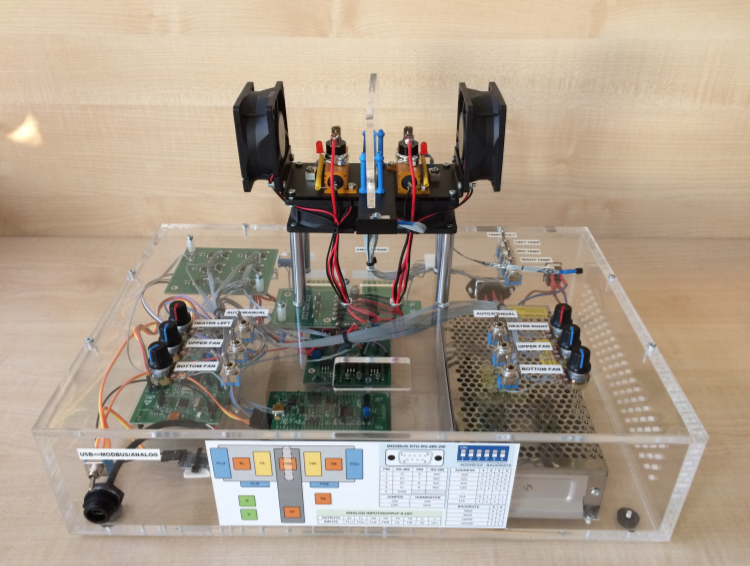
\includegraphics[width=0.7\textwidth]{ ./Rysunki/Stanowisko-grzewcze.png }
	\caption {Stanowisko grzejąco-chłodzące używane w trakcie laboratoriów.}
	\label{stanowisko_grzewcze}
\end{figure}


\section{Przebieg laboratorium}
Rozpoczynając pracę na stanowisku grzejąco-chłodzącym sprawdzono możliwość sterowania i~pomiaru w~komunikacji za stanowiskiem. W~szczególności sygnały sterujące wykorzystywane podczas niniejszego laboratorium W1, G1, Z oraz pomiaru T1 (elementy wykonawcze przedstawiono na rys. \ref{stanowisko_grzewcze_schemat}). Przez cały czas trwania laboratorium moc wentylatora W1 była ustawiona na 50\%, a wentylator traktowany jako cecha otoczenia. Dodatkowo sprawiał on, że temperatura grzałki
opadała szybciej, co było szczególnie przydatne pomiędzy doświadczeniami.

W ramach laboratorium należało wykonać 5 zadań:
\begin{enumerate}
	\label{lista_zadan}
  \item Odczytać wartość pomiaru temperatury dla termometru T1 dla mocy 26\% grzałki G1 w~stanie ustalonym (wyznaczyć punkt pracy).
  \item Wyznaczyć odpowiedzi skokowe toru zakłócenie-wyjście dla trzech różych zmian sygnału zakłócającego Z~rozpoczynając z~punktu pracy.
  \item Przygotować odpowiedzi skokowe wykorzystywane w~algorytmie DMC.
  \item Zaimplementować algorytm DMC do regulacji procesu stanowiska w języku MATLAB.
  \item Dobrać parametr $D^{\mathrm{z}$ dla algorytmu DMC i~przeprowadzić eksperymenty. 
\end{enumerate}


\begin{figure}[H]
		\centering
		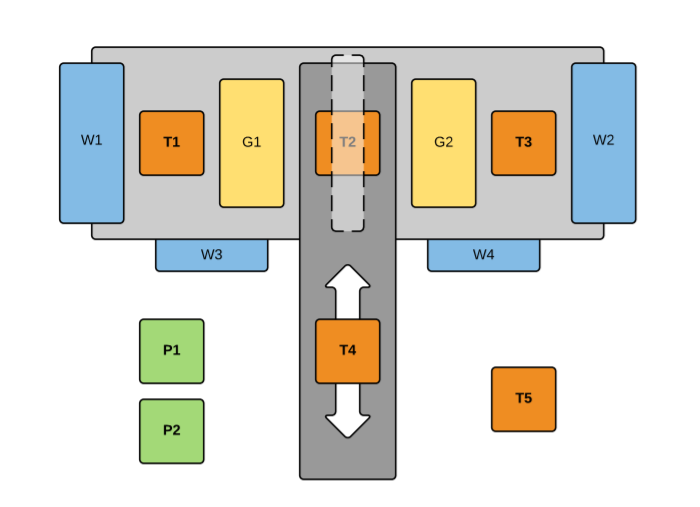
\includegraphics[width=0.7\textwidth]{ ./Rysunki/Stanowisko-grzewcze-schemat.png }
		\caption {Schemat stanowiska grzejąco-chłodzącego; zaznaczone elementy wykonawcze: wentylatory W1, W2, W3, W4, grzałki G1, G2, czujniki temperatury T1, T2, T3, T4, T5 (temperatura
otoczenia), pomiar prądu P1, pomiar napięcia P2.}
		\label{stanowisko_grzewcze_schemat}
\end{figure}

\section{Punkt pracy stanowiska}
W celu wyznaczenia punktu pracy stanowiska dla mocy grzałki G1=26\% zadano tę wartość dla sygnału sterującego grzałką. Następnie poczekano, aż temperatura T1 ustali się. Wynik eksperymentu przedstawiono na rys. \ref{punkt_pracy}. Odczytana wartość temperatury dla termometru T1 wyniosła \num{28.12} °C.


\begin{figure}[H]
	\centering
	% This file was created by matlab2tikz.
%
\definecolor{mycolor1}{rgb}{0.00000,0.44700,0.74100}%
\definecolor{mycolor2}{rgb}{0.85000,0.32500,0.09800}%
%
\begin{tikzpicture}

\begin{axis}[%
width=4.521in,
height=3.566in,
at={(0.758in,0.481in)},
scale only axis,
xmin=0,
xmax=367,
xlabel style={font=\color{white!15!black}},
xlabel={Czas [s]},
ymin=33,
ymax=36,
ylabel style={font=\color{white!15!black}},
ylabel={$\text{Temperatura [}^\circ\text{C]}$},
axis background/.style={fill=white},
title style={font=\bfseries},
title={$\text{Punkt pracy (T1 = 33,25}^\circ\text{C; T2 = 34,68}^\circ\text{C)}$},
legend style={legend cell align=left, align=left, draw=white!15!black}
]
\addplot [color=mycolor1]
  table[row sep=crcr]{%
1	34.06\\
2	34.06\\
3	34.06\\
4	34.06\\
5	34.06\\
6	34.06\\
7	34\\
8	34\\
9	34\\
10	34\\
11	33.93\\
12	33.93\\
13	33.93\\
14	33.93\\
15	33.93\\
16	33.93\\
17	33.93\\
18	33.93\\
19	33.87\\
20	33.87\\
21	33.87\\
22	33.87\\
23	33.87\\
24	33.87\\
25	33.87\\
26	33.87\\
27	33.87\\
28	33.87\\
29	33.87\\
30	33.87\\
31	33.81\\
32	33.81\\
33	33.87\\
34	33.87\\
35	33.81\\
36	33.81\\
37	33.81\\
38	33.81\\
39	33.87\\
40	33.87\\
41	33.81\\
42	33.81\\
43	33.81\\
44	33.81\\
45	33.81\\
46	33.81\\
47	33.81\\
48	33.81\\
49	33.81\\
50	33.81\\
51	33.75\\
52	33.75\\
53	33.75\\
54	33.75\\
55	33.75\\
56	33.75\\
57	33.75\\
58	33.75\\
59	33.75\\
60	33.75\\
61	33.68\\
62	33.68\\
63	33.68\\
64	33.68\\
65	33.68\\
66	33.68\\
67	33.68\\
68	33.68\\
69	33.68\\
70	33.68\\
71	33.68\\
72	33.68\\
73	33.62\\
74	33.62\\
75	33.62\\
76	33.62\\
77	33.62\\
78	33.62\\
79	33.62\\
80	33.62\\
81	33.56\\
82	33.56\\
83	33.56\\
84	33.56\\
85	33.56\\
86	33.56\\
87	33.56\\
88	33.56\\
89	33.5\\
90	33.5\\
91	33.5\\
92	33.5\\
93	33.5\\
94	33.5\\
95	33.5\\
96	33.5\\
97	33.56\\
98	33.56\\
99	33.5\\
100	33.5\\
101	33.5\\
102	33.5\\
103	33.5\\
104	33.5\\
105	33.5\\
106	33.5\\
107	33.5\\
108	33.5\\
109	33.5\\
110	33.5\\
111	33.43\\
112	33.43\\
113	33.43\\
114	33.43\\
115	33.43\\
116	33.43\\
117	33.43\\
118	33.43\\
119	33.43\\
120	33.43\\
121	33.43\\
122	33.43\\
123	33.43\\
124	33.43\\
125	33.43\\
126	33.43\\
127	33.37\\
128	33.37\\
129	33.43\\
130	33.43\\
131	33.37\\
132	33.37\\
133	33.43\\
134	33.43\\
135	33.43\\
136	33.43\\
137	33.43\\
138	33.43\\
139	33.43\\
140	33.43\\
141	33.43\\
142	33.43\\
143	33.43\\
144	33.43\\
145	33.43\\
146	33.43\\
147	33.43\\
148	33.43\\
149	33.43\\
150	33.43\\
151	33.43\\
152	33.43\\
153	33.43\\
154	33.43\\
155	33.43\\
156	33.43\\
157	33.43\\
158	33.43\\
159	33.43\\
160	33.43\\
161	33.43\\
162	33.43\\
163	33.37\\
164	33.37\\
165	33.37\\
166	33.37\\
167	33.43\\
168	33.43\\
169	33.43\\
170	33.43\\
171	33.43\\
172	33.43\\
173	33.37\\
174	33.37\\
175	33.37\\
176	33.37\\
177	33.37\\
178	33.37\\
179	33.37\\
180	33.37\\
181	33.37\\
182	33.37\\
183	33.37\\
184	33.37\\
185	33.37\\
186	33.37\\
187	33.37\\
188	33.37\\
189	33.37\\
190	33.37\\
191	33.37\\
192	33.37\\
193	33.37\\
194	33.37\\
195	33.37\\
196	33.37\\
197	33.37\\
198	33.37\\
199	33.37\\
200	33.37\\
201	33.37\\
202	33.37\\
203	33.37\\
204	33.37\\
205	33.37\\
206	33.37\\
207	33.37\\
208	33.37\\
209	33.37\\
210	33.37\\
211	33.37\\
212	33.37\\
213	33.31\\
214	33.31\\
215	33.37\\
216	33.37\\
217	33.31\\
218	33.31\\
219	33.31\\
220	33.31\\
221	33.31\\
222	33.31\\
223	33.31\\
224	33.31\\
225	33.31\\
226	33.31\\
227	33.31\\
228	33.31\\
229	33.31\\
230	33.31\\
231	33.31\\
232	33.31\\
233	33.31\\
234	33.31\\
235	33.31\\
236	33.31\\
237	33.31\\
238	33.31\\
239	33.31\\
240	33.31\\
241	33.31\\
242	33.31\\
243	33.31\\
244	33.31\\
245	33.31\\
246	33.31\\
247	33.31\\
248	33.31\\
249	33.31\\
250	33.31\\
251	33.31\\
252	33.31\\
253	33.31\\
254	33.31\\
255	33.31\\
256	33.31\\
257	33.31\\
258	33.31\\
259	33.31\\
260	33.31\\
261	33.31\\
262	33.31\\
263	33.31\\
264	33.31\\
265	33.31\\
266	33.31\\
267	33.31\\
268	33.31\\
269	33.37\\
270	33.37\\
271	33.31\\
272	33.31\\
273	33.31\\
274	33.31\\
275	33.31\\
276	33.31\\
277	33.31\\
278	33.31\\
279	33.31\\
280	33.31\\
281	33.31\\
282	33.31\\
283	33.31\\
284	33.31\\
285	33.31\\
286	33.31\\
287	33.25\\
288	33.25\\
289	33.25\\
290	33.25\\
291	33.25\\
292	33.25\\
293	33.25\\
294	33.25\\
295	33.25\\
296	33.25\\
297	33.25\\
298	33.25\\
299	33.25\\
300	33.25\\
301	33.25\\
302	33.25\\
303	33.25\\
304	33.25\\
305	33.25\\
306	33.25\\
307	33.25\\
308	33.25\\
309	33.25\\
310	33.25\\
311	33.25\\
312	33.25\\
313	33.25\\
314	33.25\\
315	33.18\\
316	33.18\\
317	33.18\\
318	33.18\\
319	33.25\\
320	33.25\\
321	33.25\\
322	33.25\\
323	33.25\\
324	33.25\\
325	33.25\\
326	33.25\\
327	33.25\\
328	33.25\\
329	33.25\\
330	33.25\\
331	33.25\\
332	33.25\\
333	33.25\\
334	33.25\\
335	33.25\\
336	33.25\\
337	33.25\\
338	33.25\\
339	33.25\\
340	33.25\\
341	33.31\\
342	33.31\\
343	33.31\\
344	33.31\\
345	33.31\\
346	33.31\\
347	33.31\\
348	33.31\\
349	33.31\\
350	33.31\\
351	33.31\\
352	33.31\\
353	33.25\\
354	33.25\\
355	33.25\\
356	33.25\\
357	33.25\\
358	33.25\\
359	33.25\\
360	33.25\\
361	33.25\\
362	33.25\\
363	33.25\\
364	33.25\\
365	33.25\\
366	33.25\\
367	33.25\\
};
\addlegendentry{$\text{Temperatura T1 [}^\circ\text{C]}$}

\addplot [color=mycolor2]
  table[row sep=crcr]{%
1	35.62\\
2	35.62\\
3	35.62\\
4	35.62\\
5	35.62\\
6	35.62\\
7	35.56\\
8	35.56\\
9	35.56\\
10	35.56\\
11	35.56\\
12	35.56\\
13	35.56\\
14	35.56\\
15	35.5\\
16	35.5\\
17	35.5\\
18	35.5\\
19	35.5\\
20	35.5\\
21	35.5\\
22	35.5\\
23	35.5\\
24	35.5\\
25	35.43\\
26	35.43\\
27	35.43\\
28	35.43\\
29	35.43\\
30	35.43\\
31	35.37\\
32	35.37\\
33	35.37\\
34	35.37\\
35	35.37\\
36	35.37\\
37	35.37\\
38	35.37\\
39	35.37\\
40	35.37\\
41	35.37\\
42	35.37\\
43	35.31\\
44	35.31\\
45	35.31\\
46	35.31\\
47	35.31\\
48	35.31\\
49	35.31\\
50	35.31\\
51	35.31\\
52	35.31\\
53	35.25\\
54	35.25\\
55	35.25\\
56	35.25\\
57	35.25\\
58	35.25\\
59	35.25\\
60	35.25\\
61	35.25\\
62	35.25\\
63	35.18\\
64	35.18\\
65	35.18\\
66	35.18\\
67	35.18\\
68	35.18\\
69	35.18\\
70	35.18\\
71	35.18\\
72	35.18\\
73	35.18\\
74	35.18\\
75	35.12\\
76	35.12\\
77	35.12\\
78	35.12\\
79	35.12\\
80	35.12\\
81	35.12\\
82	35.12\\
83	35.12\\
84	35.12\\
85	35.12\\
86	35.12\\
87	35.12\\
88	35.12\\
89	35.12\\
90	35.12\\
91	35.12\\
92	35.12\\
93	35.12\\
94	35.12\\
95	35.12\\
96	35.12\\
97	35.06\\
98	35.06\\
99	35.06\\
100	35.06\\
101	35.06\\
102	35.06\\
103	35.06\\
104	35.06\\
105	35\\
106	35\\
107	35.06\\
108	35.06\\
109	35\\
110	35\\
111	35\\
112	35\\
113	35\\
114	35\\
115	34.93\\
116	34.93\\
117	34.93\\
118	34.93\\
119	35\\
120	35\\
121	34.93\\
122	34.93\\
123	34.93\\
124	34.93\\
125	34.93\\
126	34.93\\
127	34.93\\
128	34.93\\
129	34.87\\
130	34.87\\
131	34.93\\
132	34.93\\
133	34.87\\
134	34.87\\
135	34.93\\
136	34.93\\
137	34.87\\
138	34.87\\
139	34.93\\
140	34.93\\
141	34.87\\
142	34.87\\
143	34.93\\
144	34.93\\
145	34.87\\
146	34.87\\
147	34.87\\
148	34.87\\
149	34.87\\
150	34.87\\
151	34.87\\
152	34.87\\
153	34.87\\
154	34.87\\
155	34.87\\
156	34.87\\
157	34.81\\
158	34.81\\
159	34.87\\
160	34.87\\
161	34.87\\
162	34.87\\
163	34.87\\
164	34.87\\
165	34.87\\
166	34.87\\
167	34.87\\
168	34.87\\
169	34.87\\
170	34.87\\
171	34.81\\
172	34.81\\
173	34.87\\
174	34.87\\
175	34.87\\
176	34.87\\
177	34.87\\
178	34.87\\
179	34.87\\
180	34.87\\
181	34.81\\
182	34.81\\
183	34.87\\
184	34.87\\
185	34.87\\
186	34.87\\
187	34.87\\
188	34.87\\
189	34.87\\
190	34.87\\
191	34.81\\
192	34.81\\
193	34.81\\
194	34.81\\
195	34.81\\
196	34.81\\
197	34.81\\
198	34.81\\
199	34.81\\
200	34.81\\
201	34.81\\
202	34.81\\
203	34.81\\
204	34.81\\
205	34.81\\
206	34.81\\
207	34.81\\
208	34.81\\
209	34.81\\
210	34.81\\
211	34.81\\
212	34.81\\
213	34.81\\
214	34.81\\
215	34.81\\
216	34.81\\
217	34.81\\
218	34.81\\
219	34.81\\
220	34.81\\
221	34.81\\
222	34.81\\
223	34.81\\
224	34.81\\
225	34.81\\
226	34.81\\
227	34.81\\
228	34.81\\
229	34.81\\
230	34.81\\
231	34.87\\
232	34.87\\
233	34.81\\
234	34.81\\
235	34.87\\
236	34.87\\
237	34.87\\
238	34.87\\
239	34.87\\
240	34.87\\
241	34.87\\
242	34.87\\
243	34.87\\
244	34.87\\
245	34.81\\
246	34.81\\
247	34.81\\
248	34.81\\
249	34.81\\
250	34.81\\
251	34.81\\
252	34.81\\
253	34.81\\
254	34.81\\
255	34.81\\
256	34.81\\
257	34.81\\
258	34.81\\
259	34.81\\
260	34.81\\
261	34.81\\
262	34.81\\
263	34.81\\
264	34.81\\
265	34.81\\
266	34.81\\
267	34.81\\
268	34.81\\
269	34.81\\
270	34.81\\
271	34.81\\
272	34.81\\
273	34.81\\
274	34.81\\
275	34.81\\
276	34.81\\
277	34.81\\
278	34.81\\
279	34.81\\
280	34.81\\
281	34.81\\
282	34.81\\
283	34.81\\
284	34.81\\
285	34.81\\
286	34.81\\
287	34.81\\
288	34.81\\
289	34.81\\
290	34.81\\
291	34.81\\
292	34.81\\
293	34.81\\
294	34.81\\
295	34.81\\
296	34.81\\
297	34.81\\
298	34.81\\
299	34.81\\
300	34.81\\
301	34.75\\
302	34.75\\
303	34.75\\
304	34.75\\
305	34.75\\
306	34.75\\
307	34.75\\
308	34.75\\
309	34.75\\
310	34.75\\
311	34.75\\
312	34.75\\
313	34.75\\
314	34.75\\
315	34.75\\
316	34.75\\
317	34.75\\
318	34.75\\
319	34.75\\
320	34.75\\
321	34.75\\
322	34.75\\
323	34.75\\
324	34.75\\
325	34.75\\
326	34.75\\
327	34.75\\
328	34.75\\
329	34.75\\
330	34.75\\
331	34.75\\
332	34.75\\
333	34.75\\
334	34.75\\
335	34.75\\
336	34.75\\
337	34.75\\
338	34.75\\
339	34.75\\
340	34.75\\
341	34.75\\
342	34.75\\
343	34.75\\
344	34.75\\
345	34.68\\
346	34.68\\
347	34.68\\
348	34.68\\
349	34.68\\
350	34.68\\
351	34.68\\
352	34.68\\
353	34.68\\
354	34.68\\
355	34.68\\
356	34.68\\
357	34.68\\
358	34.68\\
359	34.68\\
360	34.68\\
361	34.68\\
362	34.68\\
363	34.68\\
364	34.68\\
365	34.68\\
366	34.68\\
367	34.68\\
};
\addlegendentry{$\text{Temperatura T2 [}^\circ\text{C]}$}

\end{axis}
\end{tikzpicture}%
	\caption{Ustalanie się temperatury dla punktu pracy.}
	\label{punkt_pracy}
\end{figure}

\section{Odpowiedzi skokowe toru zakłócenie-wyjście}
Dla stanowiska pracującego w ustalonym punkcie pracy (G1=26\%; T1=\num{28.12}°C) zadano 3~różne wartości skoku zakłócenia. Eksperyment wykonano dla skoków sygnału zawsze z wartości Z=0 do kolejno wartości: Z=10, Z=20 oraz Z=30. Wyniki przedstawiono na rys. \ref{skok_zak}. Różnica w początkowych wartościach temperatury T1 dla poszczególnych skoków wynika z zakłóceń powodowanch przez zmianę temperatury w pracowni laboratoryjnej oraz nagrzewania się stanowiska grzejąco-chłodzącego.


Na podstawie wyznaczonej charakterystyki statycznej dla toru zakłócenie-wyjście przedstawionej na rys. \ref{char_skok_zak} możemy stwierdzono, że właściwości statyczne są w~przybliżeniu liniowe. Wzmocenienie statyczne dla tego toru procesu wyznaczono metodą najmniejszych kwadratów i otrzymano wartość $K_{\mathrm{stat}}=0.1725$.

\begin{figure}[H]
	\centering
	% This file was created by matlab2tikz.
%
\definecolor{mycolor1}{rgb}{0.00000,0.44700,0.74100}%
\definecolor{mycolor2}{rgb}{0.85000,0.32500,0.09800}%
\definecolor{mycolor3}{rgb}{0.92900,0.69400,0.12500}%
%
\begin{tikzpicture}

\begin{axis}[%
width=4.521in,
height=3.566in,
at={(0.758in,0.481in)},
scale only axis,
xmin=0,
xmax=500,
xlabel style={font=\color{white!15!black}},
xlabel={Czas [s]},
ymin=26,
ymax=34,
ylabel style={font=\color{white!15!black}},
ylabel={$\text{Temperatura [}^\circ\text{C]}$},
axis background/.style={fill=white},
title style={font=\bfseries},
title={Odpowiedzi skokowe dla toru zakłócenie - wyjście},
axis background/.style={fill=white},
legend style={at={(0.97,0.03)}, anchor=south east, legend cell align=left, align=left, draw=white!15!black}
]
\addplot [color=mycolor1]
  table[row sep=crcr]{%
1	28.12\\
2	28.12\\
3	28.06\\
4	28.06\\
5	28.06\\
6	28.06\\
7	28.06\\
8	28.06\\
9	28\\
10	28.06\\
11	28.06\\
12	28.06\\
13	28.06\\
14	28.12\\
15	28.12\\
16	28.12\\
17	28.18\\
18	28.18\\
19	28.25\\
20	28.25\\
21	28.25\\
22	28.31\\
23	28.31\\
24	28.31\\
25	28.37\\
26	28.37\\
27	28.37\\
28	28.37\\
29	28.43\\
30	28.43\\
31	28.43\\
32	28.5\\
33	28.5\\
34	28.5\\
35	28.5\\
36	28.56\\
37	28.56\\
38	28.56\\
39	28.62\\
40	28.62\\
41	28.62\\
42	28.62\\
43	28.62\\
44	28.62\\
45	28.68\\
46	28.62\\
47	28.68\\
48	28.68\\
49	28.62\\
50	28.62\\
51	28.62\\
52	28.68\\
53	28.68\\
54	28.68\\
55	28.75\\
56	28.75\\
57	28.75\\
58	28.75\\
59	28.75\\
60	28.81\\
61	28.81\\
62	28.81\\
63	28.87\\
64	28.87\\
65	28.93\\
66	28.93\\
67	28.93\\
68	29\\
69	29\\
70	29\\
71	29\\
72	29.06\\
73	29.06\\
74	29.06\\
75	29.06\\
76	29.06\\
77	29.06\\
78	29.12\\
79	29.12\\
80	29.12\\
81	29.12\\
82	29.12\\
83	29.12\\
84	29.18\\
85	29.18\\
86	29.18\\
87	29.18\\
88	29.18\\
89	29.18\\
90	29.18\\
91	29.18\\
92	29.18\\
93	29.18\\
94	29.25\\
95	29.25\\
96	29.25\\
97	29.25\\
98	29.25\\
99	29.25\\
100	29.25\\
101	29.25\\
102	29.31\\
103	29.31\\
104	29.31\\
105	29.31\\
106	29.31\\
107	29.31\\
108	29.37\\
109	29.37\\
110	29.37\\
111	29.37\\
112	29.37\\
113	29.37\\
114	29.37\\
115	29.37\\
116	29.37\\
117	29.37\\
118	29.37\\
119	29.37\\
120	29.37\\
121	29.37\\
122	29.37\\
123	29.37\\
124	29.37\\
125	29.37\\
126	29.43\\
127	29.37\\
128	29.43\\
129	29.43\\
130	29.43\\
131	29.43\\
132	29.43\\
133	29.43\\
134	29.43\\
135	29.5\\
136	29.43\\
137	29.5\\
138	29.5\\
139	29.5\\
140	29.5\\
141	29.5\\
142	29.5\\
143	29.5\\
144	29.5\\
145	29.5\\
146	29.5\\
147	29.43\\
148	29.5\\
149	29.43\\
150	29.5\\
151	29.43\\
152	29.5\\
153	29.43\\
154	29.5\\
155	29.43\\
156	29.43\\
157	29.43\\
158	29.43\\
159	29.43\\
160	29.43\\
161	29.43\\
162	29.43\\
163	29.5\\
164	29.5\\
165	29.5\\
166	29.5\\
167	29.5\\
168	29.5\\
169	29.5\\
170	29.5\\
171	29.5\\
172	29.43\\
173	29.5\\
174	29.5\\
175	29.5\\
176	29.5\\
177	29.5\\
178	29.5\\
179	29.5\\
180	29.5\\
181	29.5\\
182	29.5\\
183	29.56\\
184	29.56\\
185	29.56\\
186	29.56\\
187	29.62\\
188	29.56\\
189	29.62\\
190	29.62\\
191	29.62\\
192	29.62\\
193	29.62\\
194	29.62\\
195	29.62\\
196	29.68\\
197	29.68\\
198	29.62\\
199	29.68\\
200	29.68\\
201	29.68\\
202	29.68\\
203	29.68\\
204	29.75\\
205	29.68\\
206	29.68\\
207	29.75\\
208	29.68\\
209	29.68\\
210	29.68\\
211	29.68\\
212	29.75\\
213	29.68\\
214	29.68\\
215	29.68\\
216	29.68\\
217	29.68\\
218	29.68\\
219	29.68\\
220	29.68\\
221	29.68\\
222	29.68\\
223	29.68\\
224	29.68\\
225	29.68\\
226	29.68\\
227	29.68\\
228	29.68\\
229	29.68\\
230	29.68\\
231	29.68\\
232	29.68\\
233	29.68\\
234	29.68\\
235	29.68\\
236	29.68\\
237	29.68\\
238	29.68\\
239	29.68\\
240	29.68\\
241	29.68\\
242	29.68\\
243	29.68\\
244	29.68\\
245	29.68\\
246	29.75\\
247	29.68\\
248	29.68\\
249	29.68\\
250	29.68\\
251	29.68\\
252	29.68\\
253	29.68\\
254	29.68\\
255	29.68\\
256	29.75\\
257	29.75\\
258	29.75\\
259	29.75\\
260	29.75\\
261	29.75\\
262	29.75\\
263	29.75\\
264	29.75\\
265	29.75\\
266	29.75\\
267	29.75\\
268	29.75\\
269	29.75\\
270	29.75\\
271	29.75\\
272	29.75\\
273	29.81\\
274	29.81\\
275	29.81\\
276	29.81\\
277	29.81\\
278	29.81\\
279	29.81\\
280	29.81\\
281	29.81\\
282	29.81\\
283	29.81\\
284	29.81\\
285	29.81\\
286	29.81\\
287	29.81\\
288	29.81\\
289	29.81\\
290	29.81\\
291	29.81\\
292	29.81\\
293	29.81\\
294	29.81\\
295	29.75\\
296	29.75\\
297	29.75\\
298	29.75\\
299	29.75\\
300	29.75\\
301	29.75\\
302	29.75\\
303	29.75\\
304	29.75\\
305	29.75\\
306	29.75\\
307	29.75\\
308	29.68\\
309	29.68\\
310	29.68\\
311	29.68\\
312	29.68\\
313	29.68\\
314	29.62\\
315	29.62\\
316	29.62\\
317	29.62\\
318	29.62\\
319	29.68\\
320	29.68\\
321	29.75\\
322	29.68\\
323	29.75\\
324	29.75\\
325	29.81\\
326	29.81\\
327	29.81\\
328	29.81\\
329	29.81\\
330	29.81\\
331	29.81\\
332	29.81\\
333	29.81\\
334	29.81\\
335	29.81\\
336	29.81\\
337	29.81\\
338	29.75\\
339	29.75\\
340	29.75\\
341	29.81\\
342	29.81\\
343	29.81\\
344	29.81\\
345	29.81\\
346	29.81\\
347	29.81\\
348	29.81\\
349	29.81\\
350	29.81\\
351	29.81\\
352	29.81\\
353	29.75\\
354	29.75\\
355	29.75\\
356	29.75\\
357	29.75\\
358	29.68\\
359	29.68\\
360	29.75\\
361	29.68\\
362	29.75\\
363	29.75\\
364	29.68\\
365	29.75\\
366	29.75\\
367	29.75\\
368	29.75\\
369	29.75\\
370	29.81\\
371	29.81\\
372	29.81\\
373	29.81\\
374	29.81\\
375	29.87\\
376	29.87\\
377	29.87\\
378	29.87\\
379	29.81\\
380	29.81\\
381	29.81\\
382	29.81\\
383	29.81\\
384	29.81\\
385	29.81\\
386	29.81\\
387	29.81\\
388	29.81\\
389	29.81\\
390	29.81\\
391	29.81\\
392	29.75\\
393	29.81\\
394	29.81\\
395	29.81\\
396	29.81\\
397	29.81\\
398	29.81\\
399	29.81\\
400	29.81\\
401	29.81\\
402	29.81\\
403	29.81\\
404	29.81\\
405	29.81\\
406	29.81\\
407	29.87\\
408	29.81\\
409	29.81\\
410	29.81\\
411	29.81\\
412	29.81\\
413	29.81\\
414	29.81\\
415	29.81\\
416	29.81\\
417	29.75\\
418	29.75\\
419	29.75\\
420	29.75\\
421	29.75\\
422	29.75\\
423	29.75\\
424	29.75\\
425	29.75\\
426	29.75\\
427	29.75\\
428	29.75\\
429	29.75\\
430	29.75\\
431	29.75\\
432	29.75\\
433	29.75\\
434	29.75\\
435	29.75\\
436	29.75\\
437	29.75\\
438	29.75\\
439	29.75\\
440	29.75\\
441	29.75\\
442	29.75\\
443	29.75\\
444	29.68\\
445	29.68\\
446	29.75\\
447	29.68\\
448	29.75\\
449	29.75\\
450	29.75\\
451	29.75\\
452	29.75\\
453	29.75\\
454	29.81\\
455	29.75\\
456	29.75\\
457	29.75\\
458	29.75\\
459	29.75\\
460	29.75\\
461	29.75\\
462	29.75\\
463	29.75\\
464	29.75\\
465	29.81\\
466	29.81\\
467	29.81\\
468	29.81\\
469	29.81\\
470	29.81\\
471	29.81\\
472	29.81\\
473	29.81\\
474	29.81\\
475	29.81\\
476	29.81\\
477	29.81\\
478	29.81\\
479	29.81\\
480	29.81\\
481	29.81\\
482	29.81\\
483	29.81\\
484	29.81\\
485	29.81\\
486	29.87\\
487	29.87\\
488	29.87\\
489	29.87\\
490	29.93\\
491	29.93\\
492	29.93\\
493	29.93\\
494	29.93\\
495	29.93\\
496	29.93\\
497	29.93\\
498	29.87\\
499	29.93\\
500	29.93\\
};
\addlegendentry{Z = 10}

\addplot [color=mycolor2]
  table[row sep=crcr]{%
1	26.75\\
2	26.75\\
3	26.81\\
4	26.81\\
5	26.87\\
6	26.87\\
7	26.87\\
8	26.87\\
9	26.87\\
10	26.87\\
11	26.93\\
12	26.93\\
13	26.93\\
14	27\\
15	27\\
16	27\\
17	27\\
18	27.12\\
19	27.12\\
20	27.18\\
21	27.25\\
22	27.25\\
23	27.31\\
24	27.31\\
25	27.37\\
26	27.43\\
27	27.43\\
28	27.5\\
29	27.56\\
30	27.62\\
31	27.62\\
32	27.68\\
33	27.75\\
34	27.81\\
35	27.81\\
36	27.87\\
37	27.93\\
38	27.93\\
39	27.93\\
40	28\\
41	28.06\\
42	28.06\\
43	28.12\\
44	28.18\\
45	28.18\\
46	28.25\\
47	28.25\\
48	28.31\\
49	28.31\\
50	28.37\\
51	28.37\\
52	28.43\\
53	28.43\\
54	28.5\\
55	28.5\\
56	28.56\\
57	28.56\\
58	28.62\\
59	28.68\\
60	28.68\\
61	28.75\\
62	28.81\\
63	28.81\\
64	28.87\\
65	28.87\\
66	28.93\\
67	28.93\\
68	29\\
69	29.06\\
70	29.06\\
71	29.12\\
72	29.12\\
73	29.12\\
74	29.18\\
75	29.25\\
76	29.25\\
77	29.25\\
78	29.31\\
79	29.31\\
80	29.31\\
81	29.37\\
82	29.37\\
83	29.43\\
84	29.43\\
85	29.5\\
86	29.5\\
87	29.5\\
88	29.56\\
89	29.56\\
90	29.56\\
91	29.62\\
92	29.62\\
93	29.62\\
94	29.68\\
95	29.68\\
96	29.68\\
97	29.75\\
98	29.75\\
99	29.75\\
100	29.81\\
101	29.81\\
102	29.81\\
103	29.81\\
104	29.81\\
105	29.87\\
106	29.87\\
107	29.87\\
108	29.87\\
109	29.93\\
110	30\\
111	30\\
112	30.06\\
113	30.06\\
114	30.06\\
115	30.12\\
116	30.12\\
117	30.12\\
118	30.18\\
119	30.18\\
120	30.18\\
121	30.18\\
122	30.18\\
123	30.18\\
124	30.18\\
125	30.25\\
126	30.25\\
127	30.25\\
128	30.25\\
129	30.31\\
130	30.31\\
131	30.31\\
132	30.31\\
133	30.37\\
134	30.37\\
135	30.37\\
136	30.37\\
137	30.37\\
138	30.37\\
139	30.37\\
140	30.37\\
141	30.37\\
142	30.37\\
143	30.31\\
144	30.37\\
145	30.37\\
146	30.37\\
147	30.37\\
148	30.37\\
149	30.43\\
150	30.43\\
151	30.43\\
152	30.43\\
153	30.43\\
154	30.43\\
155	30.43\\
156	30.5\\
157	30.5\\
158	30.5\\
159	30.5\\
160	30.5\\
161	30.5\\
162	30.56\\
163	30.56\\
164	30.56\\
165	30.56\\
166	30.62\\
167	30.56\\
168	30.62\\
169	30.62\\
170	30.62\\
171	30.62\\
172	30.62\\
173	30.62\\
174	30.62\\
175	30.62\\
176	30.62\\
177	30.62\\
178	30.68\\
179	30.68\\
180	30.68\\
181	30.68\\
182	30.68\\
183	30.68\\
184	30.68\\
185	30.68\\
186	30.68\\
187	30.68\\
188	30.68\\
189	30.68\\
190	30.68\\
191	30.68\\
192	30.75\\
193	30.75\\
194	30.75\\
195	30.75\\
196	30.75\\
197	30.75\\
198	30.75\\
199	30.75\\
200	30.81\\
201	30.75\\
202	30.75\\
203	30.81\\
204	30.81\\
205	30.81\\
206	30.81\\
207	30.87\\
208	30.87\\
209	30.87\\
210	30.87\\
211	30.87\\
212	30.81\\
213	30.81\\
214	30.81\\
215	30.81\\
216	30.81\\
217	30.75\\
218	30.75\\
219	30.75\\
220	30.75\\
221	30.75\\
222	30.75\\
223	30.81\\
224	30.81\\
225	30.81\\
226	30.75\\
227	30.75\\
228	30.81\\
229	30.81\\
230	30.81\\
231	30.81\\
232	30.87\\
233	30.87\\
234	30.87\\
235	30.93\\
236	30.93\\
237	30.93\\
238	30.93\\
239	31\\
240	31\\
241	31\\
242	31\\
243	31\\
244	31\\
245	31\\
246	31\\
247	31.06\\
248	31\\
249	31.06\\
250	31.06\\
251	31.06\\
252	31.06\\
253	31.06\\
254	31.06\\
255	31.06\\
256	31.06\\
257	31.06\\
258	31.06\\
259	31.06\\
260	31.06\\
261	31.06\\
262	31.06\\
263	31.06\\
264	31.06\\
265	31.06\\
266	31.06\\
267	31.12\\
268	31.12\\
269	31.12\\
270	31.12\\
271	31.12\\
272	31.12\\
273	31.18\\
274	31.18\\
275	31.18\\
276	31.18\\
277	31.18\\
278	31.18\\
279	31.18\\
280	31.18\\
281	31.18\\
282	31.18\\
283	31.18\\
284	31.25\\
285	31.25\\
286	31.25\\
287	31.25\\
288	31.25\\
289	31.25\\
290	31.25\\
291	31.25\\
292	31.25\\
293	31.25\\
294	31.31\\
295	31.25\\
296	31.31\\
297	31.31\\
298	31.25\\
299	31.31\\
300	31.31\\
301	31.31\\
302	31.31\\
303	31.31\\
304	31.31\\
305	31.31\\
306	31.31\\
307	31.31\\
308	31.31\\
309	31.31\\
310	31.31\\
311	31.31\\
312	31.31\\
313	31.31\\
314	31.31\\
315	31.31\\
316	31.25\\
317	31.31\\
318	31.25\\
319	31.25\\
320	31.25\\
321	31.25\\
322	31.25\\
323	31.25\\
324	31.25\\
325	31.25\\
326	31.25\\
327	31.25\\
328	31.25\\
329	31.18\\
330	31.25\\
331	31.25\\
332	31.25\\
333	31.25\\
334	31.25\\
335	31.25\\
336	31.25\\
337	31.25\\
338	31.25\\
339	31.25\\
340	31.25\\
341	31.25\\
342	31.25\\
343	31.25\\
344	31.25\\
345	31.25\\
346	31.25\\
347	31.31\\
348	31.31\\
349	31.31\\
350	31.31\\
351	31.31\\
352	31.37\\
353	31.31\\
354	31.37\\
355	31.37\\
356	31.37\\
357	31.37\\
358	31.37\\
359	31.31\\
360	31.31\\
361	31.37\\
362	31.31\\
363	31.31\\
364	31.31\\
365	31.31\\
366	31.31\\
367	31.31\\
368	31.31\\
369	31.31\\
370	31.31\\
371	31.31\\
372	31.31\\
373	31.31\\
374	31.31\\
375	31.31\\
376	31.31\\
377	31.31\\
378	31.31\\
379	31.31\\
380	31.31\\
381	31.31\\
382	31.31\\
383	31.37\\
384	31.31\\
385	31.31\\
386	31.31\\
387	31.31\\
388	31.31\\
389	31.31\\
390	31.31\\
391	31.31\\
392	31.31\\
393	31.31\\
394	31.31\\
395	31.31\\
396	31.31\\
397	31.31\\
398	31.37\\
399	31.37\\
400	31.37\\
401	31.37\\
402	31.37\\
403	31.37\\
404	31.43\\
405	31.43\\
406	31.43\\
407	31.43\\
408	31.43\\
409	31.43\\
410	31.43\\
411	31.43\\
412	31.43\\
413	31.43\\
414	31.43\\
415	31.43\\
416	31.43\\
417	31.43\\
418	31.5\\
419	31.5\\
420	31.43\\
421	31.43\\
422	31.43\\
423	31.37\\
424	31.43\\
425	31.37\\
426	31.37\\
427	31.43\\
428	31.37\\
429	31.37\\
430	31.37\\
431	31.43\\
432	31.43\\
433	31.43\\
434	31.43\\
435	31.43\\
436	31.43\\
437	31.43\\
438	31.43\\
439	31.43\\
440	31.43\\
441	31.43\\
442	31.43\\
443	31.43\\
444	31.43\\
445	31.43\\
446	31.43\\
447	31.43\\
448	31.43\\
449	31.43\\
450	31.43\\
451	31.43\\
452	31.43\\
453	31.43\\
454	31.43\\
455	31.43\\
456	31.43\\
457	31.43\\
458	31.43\\
459	31.5\\
460	31.43\\
461	31.43\\
462	31.43\\
463	31.43\\
464	31.43\\
465	31.43\\
466	31.43\\
467	31.43\\
468	31.43\\
469	31.43\\
470	31.43\\
471	31.43\\
472	31.37\\
473	31.37\\
474	31.43\\
475	31.43\\
476	31.43\\
477	31.37\\
478	31.43\\
479	31.37\\
480	31.43\\
481	31.43\\
482	31.43\\
483	31.43\\
484	31.43\\
485	31.43\\
486	31.5\\
487	31.5\\
488	31.5\\
489	31.5\\
490	31.5\\
491	31.5\\
492	31.5\\
493	31.5\\
494	31.5\\
495	31.5\\
496	31.5\\
497	31.5\\
498	31.43\\
499	31.43\\
500	31.43\\
};
\addlegendentry{Z = 20}

\addplot [color=mycolor3]
  table[row sep=crcr]{%
1	27.93\\
2	27.93\\
3	27.93\\
4	27.93\\
5	27.93\\
6	27.93\\
7	27.93\\
8	27.93\\
9	27.93\\
10	27.93\\
11	27.93\\
12	27.93\\
13	28\\
14	28\\
15	28\\
16	28\\
17	28.06\\
18	28.06\\
19	28.12\\
20	28.18\\
21	28.18\\
22	28.25\\
23	28.37\\
24	28.37\\
25	28.43\\
26	28.5\\
27	28.56\\
28	28.62\\
29	28.62\\
30	28.68\\
31	28.75\\
32	28.81\\
33	28.87\\
34	28.93\\
35	28.93\\
36	29\\
37	29.06\\
38	29.12\\
39	29.18\\
40	29.18\\
41	29.25\\
42	29.31\\
43	29.37\\
44	29.43\\
45	29.43\\
46	29.5\\
47	29.56\\
48	29.62\\
49	29.68\\
50	29.68\\
51	29.75\\
52	29.81\\
53	29.87\\
54	30\\
55	30\\
56	30.06\\
57	30.12\\
58	30.12\\
59	30.18\\
60	30.25\\
61	30.31\\
62	30.31\\
63	30.37\\
64	30.37\\
65	30.43\\
66	30.5\\
67	30.56\\
68	30.56\\
69	30.62\\
70	30.62\\
71	30.68\\
72	30.68\\
73	30.75\\
74	30.81\\
75	30.87\\
76	30.87\\
77	30.93\\
78	30.93\\
79	31\\
80	31\\
81	31\\
82	31\\
83	31\\
84	31.06\\
85	31.06\\
86	31.12\\
87	31.12\\
88	31.18\\
89	31.18\\
90	31.18\\
91	31.25\\
92	31.25\\
93	31.25\\
94	31.25\\
95	31.25\\
96	31.31\\
97	31.31\\
98	31.31\\
99	31.31\\
100	31.37\\
101	31.37\\
102	31.37\\
103	31.37\\
104	31.37\\
105	31.37\\
106	31.43\\
107	31.43\\
108	31.5\\
109	31.5\\
110	31.5\\
111	31.5\\
112	31.56\\
113	31.56\\
114	31.56\\
115	31.56\\
116	31.56\\
117	31.56\\
118	31.56\\
119	31.56\\
120	31.62\\
121	31.62\\
122	31.62\\
123	31.62\\
124	31.68\\
125	31.68\\
126	31.75\\
127	31.75\\
128	31.75\\
129	31.75\\
130	31.81\\
131	31.81\\
132	31.87\\
133	31.87\\
134	31.87\\
135	31.87\\
136	31.87\\
137	31.93\\
138	31.93\\
139	31.93\\
140	31.93\\
141	31.93\\
142	31.93\\
143	31.93\\
144	31.93\\
145	32\\
146	31.93\\
147	32\\
148	32\\
149	31.93\\
150	31.93\\
151	32\\
152	32\\
153	32\\
154	32\\
155	32.06\\
156	32.06\\
157	32.12\\
158	32.12\\
159	32.12\\
160	32.18\\
161	32.18\\
162	32.18\\
163	32.18\\
164	32.25\\
165	32.25\\
166	32.31\\
167	32.31\\
168	32.31\\
169	32.31\\
170	32.25\\
171	32.25\\
172	32.31\\
173	32.25\\
174	32.25\\
175	32.25\\
176	32.25\\
177	32.25\\
178	32.25\\
179	32.25\\
180	32.31\\
181	32.25\\
182	32.31\\
183	32.31\\
184	32.37\\
185	32.31\\
186	32.31\\
187	32.37\\
188	32.37\\
189	32.37\\
190	32.31\\
191	32.31\\
192	32.37\\
193	32.37\\
194	32.43\\
195	32.43\\
196	32.43\\
197	32.43\\
198	32.5\\
199	32.5\\
200	32.56\\
201	32.56\\
202	32.56\\
203	32.56\\
204	32.62\\
205	32.62\\
206	32.62\\
207	32.62\\
208	32.62\\
209	32.62\\
210	32.68\\
211	32.68\\
212	32.68\\
213	32.68\\
214	32.68\\
215	32.68\\
216	32.68\\
217	32.75\\
218	32.75\\
219	32.75\\
220	32.75\\
221	32.75\\
222	32.75\\
223	32.75\\
224	32.68\\
225	32.75\\
226	32.68\\
227	32.68\\
228	32.75\\
229	32.68\\
230	32.75\\
231	32.75\\
232	32.75\\
233	32.75\\
234	32.68\\
235	32.68\\
236	32.68\\
237	32.68\\
238	32.68\\
239	32.68\\
240	32.75\\
241	32.75\\
242	32.75\\
243	32.68\\
244	32.68\\
245	32.68\\
246	32.68\\
247	32.68\\
248	32.68\\
249	32.68\\
250	32.68\\
251	32.75\\
252	32.75\\
253	32.75\\
254	32.75\\
255	32.81\\
256	32.81\\
257	32.87\\
258	32.87\\
259	32.87\\
260	32.87\\
261	32.87\\
262	32.87\\
263	32.87\\
264	32.93\\
265	32.93\\
266	32.93\\
267	32.93\\
268	32.93\\
269	32.93\\
270	32.93\\
271	32.93\\
272	32.87\\
273	32.87\\
274	32.87\\
275	32.87\\
276	32.87\\
277	32.93\\
278	32.87\\
279	32.93\\
280	32.87\\
281	32.93\\
282	32.87\\
283	32.87\\
284	32.87\\
285	32.87\\
286	32.87\\
287	32.87\\
288	32.93\\
289	32.93\\
290	32.93\\
291	32.93\\
292	32.93\\
293	33\\
294	32.93\\
295	32.93\\
296	33\\
297	32.93\\
298	33\\
299	32.93\\
300	32.93\\
301	32.93\\
302	33\\
303	33\\
304	33\\
305	33\\
306	33\\
307	33\\
308	33\\
309	33\\
310	33.06\\
311	33.06\\
312	33.06\\
313	33.06\\
314	33.12\\
315	33.12\\
316	33.12\\
317	33.12\\
318	33.12\\
319	33.12\\
320	33.12\\
321	33.12\\
322	33.12\\
323	33.12\\
324	33.12\\
325	33.06\\
326	33.12\\
327	33.06\\
328	33.06\\
329	33.06\\
330	33.06\\
331	33.06\\
332	33.06\\
333	33.06\\
334	33\\
335	33\\
336	33\\
337	33\\
338	33.06\\
339	33.06\\
340	33.06\\
341	33.12\\
342	33.12\\
343	33.12\\
344	33.12\\
345	33.12\\
346	33.12\\
347	33.12\\
348	33.12\\
349	33.12\\
350	33.12\\
351	33.18\\
352	33.12\\
353	33.18\\
354	33.18\\
355	33.18\\
356	33.18\\
357	33.18\\
358	33.18\\
359	33.25\\
360	33.25\\
361	33.18\\
362	33.25\\
363	33.25\\
364	33.25\\
365	33.25\\
366	33.25\\
367	33.31\\
368	33.31\\
369	33.31\\
370	33.31\\
371	33.31\\
372	33.31\\
373	33.31\\
374	33.31\\
375	33.31\\
376	33.31\\
377	33.31\\
378	33.37\\
379	33.37\\
380	33.37\\
381	33.37\\
382	33.37\\
383	33.37\\
384	33.43\\
385	33.43\\
386	33.37\\
387	33.37\\
388	33.37\\
389	33.37\\
390	33.31\\
391	33.31\\
392	33.31\\
393	33.25\\
394	33.25\\
395	33.25\\
396	33.25\\
397	33.31\\
398	33.31\\
399	33.25\\
400	33.25\\
401	33.25\\
402	33.25\\
403	33.25\\
404	33.25\\
405	33.25\\
406	33.25\\
407	33.25\\
408	33.25\\
409	33.25\\
410	33.25\\
411	33.31\\
412	33.25\\
413	33.25\\
414	33.31\\
415	33.31\\
416	33.31\\
417	33.31\\
418	33.31\\
419	33.37\\
420	33.37\\
421	33.37\\
422	33.37\\
423	33.43\\
424	33.37\\
425	33.43\\
426	33.43\\
427	33.43\\
428	33.37\\
429	33.37\\
430	33.37\\
431	33.37\\
432	33.37\\
433	33.37\\
434	33.31\\
435	33.31\\
436	33.31\\
437	33.31\\
438	33.31\\
439	33.31\\
440	33.25\\
441	33.25\\
442	33.25\\
443	33.18\\
444	33.18\\
445	33.18\\
446	33.18\\
447	33.12\\
448	33.12\\
449	33.18\\
450	33.18\\
451	33.18\\
452	33.12\\
453	33.12\\
454	33.12\\
455	33.12\\
456	33.12\\
457	33.12\\
458	33.18\\
459	33.18\\
460	33.18\\
461	33.18\\
462	33.25\\
463	33.25\\
464	33.25\\
465	33.25\\
466	33.31\\
467	33.31\\
468	33.31\\
469	33.31\\
470	33.31\\
471	33.37\\
472	33.37\\
473	33.37\\
474	33.37\\
475	33.37\\
476	33.37\\
477	33.37\\
478	33.37\\
479	33.37\\
480	33.31\\
481	33.31\\
482	33.31\\
483	33.31\\
484	33.31\\
485	33.31\\
486	33.31\\
487	33.31\\
488	33.31\\
489	33.31\\
490	33.31\\
491	33.31\\
492	33.31\\
493	33.31\\
494	33.31\\
495	33.37\\
496	33.37\\
497	33.37\\
498	33.43\\
499	33.43\\
500	33.43\\
};
\addlegendentry{Z = 30}

\end{axis}
\end{tikzpicture}%
	\caption{Odpowiedzi skokowe dla toru zakłócenie - wyjście.}
	\label{skok_zak}
\end{figure}

\begin{figure}[H]
	\centering
	% This file was created by matlab2tikz.
%
\definecolor{mycolor1}{rgb}{0.00000,0.44700,0.74100}%
\definecolor{mycolor2}{rgb}{0.85000,0.32500,0.09800}%
%
\begin{tikzpicture}

\begin{axis}[%
width=4.521in,
height=3.566in,
at={(0.758in,0.481in)},
scale only axis,
xmin=0,
xmax=30,
xlabel style={font=\color{white!15!black}},
xlabel={Zakłócenie},
ymin=28,
ymax=34,
ylabel style={font=\color{white!15!black}},
ylabel={$\text{Wyjście procesu (T1) [}^\circ\text{C]}$},
axis background/.style={fill=white},
title style={font=\bfseries},
title={$\text{Wzmocnienie statyczne toru zakłócenie-wyjście; K}_{\text{stat}}\text{ = 0.1725}$},
axis background/.style={fill=white},
]
\addplot [color=mycolor1, forget plot]
  table[row sep=crcr]{%
0	28.12\\
10	29.93\\
20	31.43\\
30	33.37\\
};
\addplot [color=mycolor2, only marks, mark=o, mark options={solid, mycolor2}, forget plot]
  table[row sep=crcr]{%
0	28.12\\
10	29.93\\
20	31.43\\
30	33.37\\
};
\end{axis}
\end{tikzpicture}%
	\caption{Charakterystyka statyczna dla toru zakłócenie - wyjście.}
	\label{char_skok_zak}
\end{figure}

\section{Odpowiedzi skokowe dla algorytmu DMC}
W celu wyznaczenia odpowiedzi skokowej toru zakłócenie-wyjście wybrano trzecią odpowiedź skokową przedstawioną na rys. \ref{skok_zak}, tj. skok zakłócenia do wartości Z=30. Do przekształcenia zebranej odpowiedzi skokowej skorzystano z przekształcenia:

\begin{equation}
	S(i)= \frac{Y(i) - Y_{\mathrm{pp}}}{Z_{\mathrm{skok}} - Z_{\mathrm{pp}}}
\end{equation}
gdzie:
\begin{itemize}
  \item $S(i)$ - odpowiedź skokowa potrzebna do algorytmu DMC,
	\item $Y(i)$ - odpowiedź skokowa przed przekształceniem,
	\item $Y_{\mathrm{pp}}$ - wartość wyjścia w chwili k=0 (tutaj $Y_{\mathrm{pp}}$  = \num{27.93}),
	\item $Z_{\mathrm{skok}}$ - wartość sterowanie w chwili k=0 i później (tutaj $Z_{\mathrm{skok}} = 30$),
	\item $Z_{\mathrm{pp}}$ - wartość sterowania przed chwilą k=0 (tutaj $Z_{\mathrm{pp}} = 0$)
\end{itemize}

Otrzymana odpowiedź skokowa dla toru zakłócenie wyjście została przedsawiona na rys. \ref{skok_DMC_zak}. Następnie dokonano aproksymacji odpowiedzi skokowej poprzez przybliżenie używając w tym celu członu inercyjnego drugiego stopnia z opóźnieniem:

\begin{equation}
	G(s)= \frac{K}{(sT_1 + 1)(sT_2 + 1)}e^{-T_{\mathrm{d}}s}
\end{equation}

Po dyskretyzacji danej transmitancji otrzymujemy:
\begin{equation}
	G(z)= \frac{b_1z^{-1} + b_2z^{-2}}{1 + a_1z^{-1} + a_2z^{-2}}z^{-T_{\mathrm{d}}}
\end{equation}

gdzie:
\begin{equation}
\begin{split}
	& a_1 = -\alpha_1 - \alpha_2 \\
	& a_2 = \alpha_1\alpha_2 \\
	& \alpha_1 = e^{-\frac{1}{T_1}} \\
	& \alpha_2 = e^{-\frac{1}{T_2}} \\
	& b_1 = \frac{K}{T_1 - T_2}[T_1(1-\alpha_1) - T_2(1-\alpha_2)] \\
	& b_2 = \frac{K}{T_1 - T_2}[\alpha_1T_2(1-\alpha_2) - \alpha_2T_1(1-\alpha_1)]
\end{split}
\end{equation}

Dla otrzymanej w~ten sposób transmitancji w~postaci dyskretnej napisano funkcję \\\verb+AproksSkokZak_DMC(X)+, która przyjmowała parametry $T_{\mathrm{1}}$, $T_{\mathrm{2}}$ oraz $K$. Wartość parametru \\$T_{\mathrm{d}}=12$ odczytano z odpowiedzi skokwej, ponieważ jest to opóźnienie. Funkcja ta zwracała sumaryczny błąd kwadratowy pomiędzy aproksymacją otrzymaną dla zadanych parametrów a eksperymentalnie wyznaczoną odpowiedzią skokową dla toru zakłócenie-wyjście po przekształceniu dla algorytmu regulacji DMC.  Implementacja funkcji \verb+AproksSkokZak_DMC(X)+:

\lstinputlisting{../Programy/AproksSkokZak_DMC.m}

Do wyznaczenia współczynników transmitancji użyto funkcji \verb+ga+ dostępnej w programie MATLAB, która wykorzystuje algorytm generyczny do wyznaczenia minimum funkcji. Dla naszej funkcji jest to równoważne ze znalezieniem najlepiej dopasowanej aproksymacji odpowiedzi skokowej toru zakłócenie-wyjście.
Paramerty związane z algorytmem generycznym to kolejno:

\begin{equation}
	\begin{split}
		& StallGenLimit = 200 \\
		& PopulationSize = 400 \\
		& FunctionTolerance = $1e^{-8}$ \\
	\end{split}
\end{equation}

gdzie:

\begin{itemize}
	\item $StallGenLimit$ oznacza maksymalną ilość iteracji algorytmu, dla których wartość różnicy między wartościami wyniku funkcji optymalizowanej jest mniejsza niż $FunctionTolerance$.
	\item $PopulationSize$ oznacza ilość ziaren dla algorytmu generytecznego w każdej iteracji.
	\item $FunctionTolerance$ oznacza wartość wskaźnika toleracji, który determinuje dla jakiej dokładoności algorytm uznaje, że otrzymany wynik jest ostateczy.
\end{itemize}

Wybrane wartości powyższych parametrów pozwalają na aproksymację z małym błędem, co sprawdzono poprzez kilkukrotne wywołanie algorytmu i dostrojenie eksperymentalne parametrów. Implementacja optymalizacji:

\lstinputlisting{../Programy/Optymalizacja_S_z.m}

Ponieważ do  minimalizacji funkcji użyto algorytmu generycznego to wyniki podczas kolejnych odtworzeń mogą się różnic. Jednak po wykonaniu testów, dla których błąd aproksymacji był bardzo zbliżony przyjęto wartości parametrów:

\begin{equation}
	\begin{split}
		& K = 0.1772938\\
		& T_1 = 88.311400 \\
		& T_2 = 0.010351 \\
		& T_{\mathrm{d}} = 12 \\
	\end{split}
\end{equation}

Otrzymaną aproksymowaną odpowiedź skokową dla toru zakłócenie-wyjście dla algorytmu regulacji DMC przedstawiono na rys. \ref{skok_DMC_zak_apro}.

\begin{figure}[H]
	\centering
	% This file was created by matlab2tikz.
%
%The latest updates can be retrieved from
%  http://www.mathworks.com/matlabcentral/fileexchange/22022-matlab2tikz-matlab2tikz
%where you can also make suggestions and rate matlab2tikz.
%
\definecolor{mycolor1}{rgb}{0.00000,0.44700,0.74100}%
%
\begin{tikzpicture}

\begin{axis}[%
width=4.521in,
height=3.566in,
at={(0.758in,0.481in)},
scale only axis,
xmin=0,
xmax=500,
xlabel style={font=\color{white!15!black}},
xlabel={k},
ymin=0,
ymax=0.2,
ylabel style={font=\color{white!15!black}},
ylabel={$\text{S}_\text{z}\text{(k)}$},
axis background/.style={fill=white},
title style={font=\bfseries},
title={$\text{Odpowiedź skokowa zakłócenia dla DMC; D}_\text{z}\text{ = 500}$}
]
\addplot [color=mycolor1, forget plot]
  table[row sep=crcr]{%
1	0\\
2	0\\
3	0\\
4	0\\
5	0\\
6	0\\
7	0\\
8	0\\
9	0\\
10	0\\
11	0\\
12	0\\
13	0.00233333333333334\\
14	0.00233333333333334\\
15	0.00233333333333334\\
16	0.00233333333333334\\
17	0.0043333333333333\\
18	0.0043333333333333\\
19	0.00633333333333338\\
20	0.00833333333333333\\
21	0.00833333333333333\\
22	0.0106666666666667\\
23	0.0146666666666667\\
24	0.0146666666666667\\
25	0.0166666666666667\\
26	0.019\\
27	0.021\\
28	0.023\\
29	0.023\\
30	0.025\\
31	0.0273333333333333\\
32	0.0293333333333333\\
33	0.0313333333333334\\
34	0.0333333333333333\\
35	0.0333333333333333\\
36	0.0356666666666667\\
37	0.0376666666666666\\
38	0.0396666666666667\\
39	0.0416666666666667\\
40	0.0416666666666667\\
41	0.044\\
42	0.046\\
43	0.048\\
44	0.05\\
45	0.05\\
46	0.0523333333333333\\
47	0.0543333333333333\\
48	0.0563333333333334\\
49	0.0583333333333333\\
50	0.0583333333333333\\
51	0.0606666666666667\\
52	0.0626666666666666\\
53	0.0646666666666667\\
54	0.069\\
55	0.069\\
56	0.071\\
57	0.073\\
58	0.073\\
59	0.075\\
60	0.0773333333333333\\
61	0.0793333333333333\\
62	0.0793333333333333\\
63	0.0813333333333334\\
64	0.0813333333333334\\
65	0.0833333333333333\\
66	0.0856666666666667\\
67	0.0876666666666666\\
68	0.0876666666666666\\
69	0.0896666666666667\\
70	0.0896666666666667\\
71	0.0916666666666667\\
72	0.0916666666666667\\
73	0.094\\
74	0.096\\
75	0.098\\
76	0.098\\
77	0.1\\
78	0.1\\
79	0.102333333333333\\
80	0.102333333333333\\
81	0.102333333333333\\
82	0.102333333333333\\
83	0.102333333333333\\
84	0.104333333333333\\
85	0.104333333333333\\
86	0.106333333333333\\
87	0.106333333333333\\
88	0.108333333333333\\
89	0.108333333333333\\
90	0.108333333333333\\
91	0.110666666666667\\
92	0.110666666666667\\
93	0.110666666666667\\
94	0.110666666666667\\
95	0.110666666666667\\
96	0.112666666666667\\
97	0.112666666666667\\
98	0.112666666666667\\
99	0.112666666666667\\
100	0.114666666666667\\
101	0.114666666666667\\
102	0.114666666666667\\
103	0.114666666666667\\
104	0.114666666666667\\
105	0.114666666666667\\
106	0.116666666666667\\
107	0.116666666666667\\
108	0.119\\
109	0.119\\
110	0.119\\
111	0.119\\
112	0.121\\
113	0.121\\
114	0.121\\
115	0.121\\
116	0.121\\
117	0.121\\
118	0.121\\
119	0.121\\
120	0.123\\
121	0.123\\
122	0.123\\
123	0.123\\
124	0.125\\
125	0.125\\
126	0.127333333333333\\
127	0.127333333333333\\
128	0.127333333333333\\
129	0.127333333333333\\
130	0.129333333333333\\
131	0.129333333333333\\
132	0.131333333333333\\
133	0.131333333333333\\
134	0.131333333333333\\
135	0.131333333333333\\
136	0.131333333333333\\
137	0.133333333333333\\
138	0.133333333333333\\
139	0.133333333333333\\
140	0.133333333333333\\
141	0.133333333333333\\
142	0.133333333333333\\
143	0.133333333333333\\
144	0.133333333333333\\
145	0.135666666666667\\
146	0.133333333333333\\
147	0.135666666666667\\
148	0.135666666666667\\
149	0.133333333333333\\
150	0.133333333333333\\
151	0.135666666666667\\
152	0.135666666666667\\
153	0.135666666666667\\
154	0.135666666666667\\
155	0.137666666666667\\
156	0.137666666666667\\
157	0.139666666666667\\
158	0.139666666666667\\
159	0.139666666666667\\
160	0.141666666666667\\
161	0.141666666666667\\
162	0.141666666666667\\
163	0.141666666666667\\
164	0.144\\
165	0.144\\
166	0.146\\
167	0.146\\
168	0.146\\
169	0.146\\
170	0.144\\
171	0.144\\
172	0.146\\
173	0.144\\
174	0.144\\
175	0.144\\
176	0.144\\
177	0.144\\
178	0.144\\
179	0.144\\
180	0.146\\
181	0.144\\
182	0.146\\
183	0.146\\
184	0.148\\
185	0.146\\
186	0.146\\
187	0.148\\
188	0.148\\
189	0.148\\
190	0.146\\
191	0.146\\
192	0.148\\
193	0.148\\
194	0.15\\
195	0.15\\
196	0.15\\
197	0.15\\
198	0.152333333333333\\
199	0.152333333333333\\
200	0.154333333333333\\
201	0.154333333333333\\
202	0.154333333333333\\
203	0.154333333333333\\
204	0.156333333333333\\
205	0.156333333333333\\
206	0.156333333333333\\
207	0.156333333333333\\
208	0.156333333333333\\
209	0.156333333333333\\
210	0.158333333333333\\
211	0.158333333333333\\
212	0.158333333333333\\
213	0.158333333333333\\
214	0.158333333333333\\
215	0.158333333333333\\
216	0.158333333333333\\
217	0.160666666666667\\
218	0.160666666666667\\
219	0.160666666666667\\
220	0.160666666666667\\
221	0.160666666666667\\
222	0.160666666666667\\
223	0.160666666666667\\
224	0.158333333333333\\
225	0.160666666666667\\
226	0.158333333333333\\
227	0.158333333333333\\
228	0.160666666666667\\
229	0.158333333333333\\
230	0.160666666666667\\
231	0.160666666666667\\
232	0.160666666666667\\
233	0.160666666666667\\
234	0.158333333333333\\
235	0.158333333333333\\
236	0.158333333333333\\
237	0.158333333333333\\
238	0.158333333333333\\
239	0.158333333333333\\
240	0.160666666666667\\
241	0.160666666666667\\
242	0.160666666666667\\
243	0.158333333333333\\
244	0.158333333333333\\
245	0.158333333333333\\
246	0.158333333333333\\
247	0.158333333333333\\
248	0.158333333333333\\
249	0.158333333333333\\
250	0.158333333333333\\
251	0.160666666666667\\
252	0.160666666666667\\
253	0.160666666666667\\
254	0.160666666666667\\
255	0.162666666666667\\
256	0.162666666666667\\
257	0.164666666666667\\
258	0.164666666666667\\
259	0.164666666666667\\
260	0.164666666666667\\
261	0.164666666666667\\
262	0.164666666666667\\
263	0.164666666666667\\
264	0.166666666666667\\
265	0.166666666666667\\
266	0.166666666666667\\
267	0.166666666666667\\
268	0.166666666666667\\
269	0.166666666666667\\
270	0.166666666666667\\
271	0.166666666666667\\
272	0.164666666666667\\
273	0.164666666666667\\
274	0.164666666666667\\
275	0.164666666666667\\
276	0.164666666666667\\
277	0.166666666666667\\
278	0.164666666666667\\
279	0.166666666666667\\
280	0.164666666666667\\
281	0.166666666666667\\
282	0.164666666666667\\
283	0.164666666666667\\
284	0.164666666666667\\
285	0.164666666666667\\
286	0.164666666666667\\
287	0.164666666666667\\
288	0.166666666666667\\
289	0.166666666666667\\
290	0.166666666666667\\
291	0.166666666666667\\
292	0.166666666666667\\
293	0.169\\
294	0.166666666666667\\
295	0.166666666666667\\
296	0.169\\
297	0.166666666666667\\
298	0.169\\
299	0.166666666666667\\
300	0.166666666666667\\
301	0.166666666666667\\
302	0.169\\
303	0.169\\
304	0.169\\
305	0.169\\
306	0.169\\
307	0.169\\
308	0.169\\
309	0.169\\
310	0.171\\
311	0.171\\
312	0.171\\
313	0.171\\
314	0.173\\
315	0.173\\
316	0.173\\
317	0.173\\
318	0.173\\
319	0.173\\
320	0.173\\
321	0.173\\
322	0.173\\
323	0.173\\
324	0.173\\
325	0.171\\
326	0.173\\
327	0.171\\
328	0.171\\
329	0.171\\
330	0.171\\
331	0.171\\
332	0.171\\
333	0.171\\
334	0.169\\
335	0.169\\
336	0.169\\
337	0.169\\
338	0.171\\
339	0.171\\
340	0.171\\
341	0.173\\
342	0.173\\
343	0.173\\
344	0.173\\
345	0.173\\
346	0.173\\
347	0.173\\
348	0.173\\
349	0.173\\
350	0.173\\
351	0.175\\
352	0.173\\
353	0.175\\
354	0.175\\
355	0.175\\
356	0.175\\
357	0.175\\
358	0.175\\
359	0.177333333333333\\
360	0.177333333333333\\
361	0.175\\
362	0.177333333333333\\
363	0.177333333333333\\
364	0.177333333333333\\
365	0.177333333333333\\
366	0.177333333333333\\
367	0.179333333333333\\
368	0.179333333333333\\
369	0.179333333333333\\
370	0.179333333333333\\
371	0.179333333333333\\
372	0.179333333333333\\
373	0.179333333333333\\
374	0.179333333333333\\
375	0.179333333333333\\
376	0.179333333333333\\
377	0.179333333333333\\
378	0.181333333333333\\
379	0.181333333333333\\
380	0.181333333333333\\
381	0.181333333333333\\
382	0.181333333333333\\
383	0.181333333333333\\
384	0.183333333333333\\
385	0.183333333333333\\
386	0.181333333333333\\
387	0.181333333333333\\
388	0.181333333333333\\
389	0.181333333333333\\
390	0.179333333333333\\
391	0.179333333333333\\
392	0.179333333333333\\
393	0.177333333333333\\
394	0.177333333333333\\
395	0.177333333333333\\
396	0.177333333333333\\
397	0.179333333333333\\
398	0.179333333333333\\
399	0.177333333333333\\
400	0.177333333333333\\
401	0.177333333333333\\
402	0.177333333333333\\
403	0.177333333333333\\
404	0.177333333333333\\
405	0.177333333333333\\
406	0.177333333333333\\
407	0.177333333333333\\
408	0.177333333333333\\
409	0.177333333333333\\
410	0.177333333333333\\
411	0.179333333333333\\
412	0.177333333333333\\
413	0.177333333333333\\
414	0.179333333333333\\
415	0.179333333333333\\
416	0.179333333333333\\
417	0.179333333333333\\
418	0.179333333333333\\
419	0.181333333333333\\
420	0.181333333333333\\
421	0.181333333333333\\
422	0.181333333333333\\
423	0.183333333333333\\
424	0.181333333333333\\
425	0.183333333333333\\
426	0.183333333333333\\
427	0.183333333333333\\
428	0.181333333333333\\
429	0.181333333333333\\
430	0.181333333333333\\
431	0.181333333333333\\
432	0.181333333333333\\
433	0.181333333333333\\
434	0.179333333333333\\
435	0.179333333333333\\
436	0.179333333333333\\
437	0.179333333333333\\
438	0.179333333333333\\
439	0.179333333333333\\
440	0.177333333333333\\
441	0.177333333333333\\
442	0.177333333333333\\
443	0.175\\
444	0.175\\
445	0.175\\
446	0.175\\
447	0.173\\
448	0.173\\
449	0.175\\
450	0.175\\
451	0.175\\
452	0.173\\
453	0.173\\
454	0.173\\
455	0.173\\
456	0.173\\
457	0.173\\
458	0.175\\
459	0.175\\
460	0.175\\
461	0.175\\
462	0.177333333333333\\
463	0.177333333333333\\
464	0.177333333333333\\
465	0.177333333333333\\
466	0.179333333333333\\
467	0.179333333333333\\
468	0.179333333333333\\
469	0.179333333333333\\
470	0.179333333333333\\
471	0.181333333333333\\
472	0.181333333333333\\
473	0.181333333333333\\
474	0.181333333333333\\
475	0.181333333333333\\
476	0.181333333333333\\
477	0.181333333333333\\
478	0.181333333333333\\
479	0.181333333333333\\
480	0.179333333333333\\
481	0.179333333333333\\
482	0.179333333333333\\
483	0.179333333333333\\
484	0.179333333333333\\
485	0.179333333333333\\
486	0.179333333333333\\
487	0.179333333333333\\
488	0.179333333333333\\
489	0.179333333333333\\
490	0.179333333333333\\
491	0.179333333333333\\
492	0.179333333333333\\
493	0.179333333333333\\
494	0.179333333333333\\
495	0.181333333333333\\
496	0.181333333333333\\
497	0.181333333333333\\
498	0.183333333333333\\
499	0.183333333333333\\
500	0.183333333333333\\
};
\end{axis}
\end{tikzpicture}%
	\caption{Odpowiedź skokowa toru zakłócenie-wyjście dla algorytmu DMC.}
	\label{skok_DMC_zak}
\end{figure}
	
	
\begin{figure}[H]
	\centering
	% This file was created by matlab2tikz.
%
\definecolor{mycolor1}{rgb}{0.00000,0.44700,0.74100}%
\definecolor{mycolor2}{rgb}{0.85000,0.32500,0.09800}%
%
\begin{tikzpicture}

\begin{axis}[%
width=4.521in,
height=3.566in,
at={(0.758in,0.481in)},
scale only axis,
xmin=0,
xmax=500,
xlabel style={font=\color{white!15!black}},
xlabel={k},
ymin=0,
ymax=0.2,
ylabel style={font=\color{white!15!black}},
ylabel={$\text{S}_\text{z}\text{(k)}$},
axis background/.style={fill=white},
title style={font=\bfseries},
title={Aproksymacja odpowiedzi skokowej toru zakłócenie-wyjście},
axis background/.style={fill=white},
legend style={at={(0.97,0.03)}, anchor=south east, legend cell align=left, align=left, draw=white!15!black}
]
\addplot [color=mycolor1]
  table[row sep=crcr]{%
1	0\\
2	0\\
3	0\\
4	0\\
5	0\\
6	0\\
7	0\\
8	0\\
9	0\\
10	0\\
11	0\\
12	0\\
13	0.00233333333333334\\
14	0.00233333333333334\\
15	0.00233333333333334\\
16	0.00233333333333334\\
17	0.0043333333333333\\
18	0.0043333333333333\\
19	0.00633333333333338\\
20	0.00833333333333333\\
21	0.00833333333333333\\
22	0.0106666666666667\\
23	0.0146666666666667\\
24	0.0146666666666667\\
25	0.0166666666666667\\
26	0.019\\
27	0.021\\
28	0.023\\
29	0.023\\
30	0.025\\
31	0.0273333333333333\\
32	0.0293333333333333\\
33	0.0313333333333334\\
34	0.0333333333333333\\
35	0.0333333333333333\\
36	0.0356666666666667\\
37	0.0376666666666666\\
38	0.0396666666666667\\
39	0.0416666666666667\\
40	0.0416666666666667\\
41	0.044\\
42	0.046\\
43	0.048\\
44	0.05\\
45	0.05\\
46	0.0523333333333333\\
47	0.0543333333333333\\
48	0.0563333333333334\\
49	0.0583333333333333\\
50	0.0583333333333333\\
51	0.0606666666666667\\
52	0.0626666666666666\\
53	0.0646666666666667\\
54	0.069\\
55	0.069\\
56	0.071\\
57	0.073\\
58	0.073\\
59	0.075\\
60	0.0773333333333333\\
61	0.0793333333333333\\
62	0.0793333333333333\\
63	0.0813333333333334\\
64	0.0813333333333334\\
65	0.0833333333333333\\
66	0.0856666666666667\\
67	0.0876666666666666\\
68	0.0876666666666666\\
69	0.0896666666666667\\
70	0.0896666666666667\\
71	0.0916666666666667\\
72	0.0916666666666667\\
73	0.094\\
74	0.096\\
75	0.098\\
76	0.098\\
77	0.1\\
78	0.1\\
79	0.102333333333333\\
80	0.102333333333333\\
81	0.102333333333333\\
82	0.102333333333333\\
83	0.102333333333333\\
84	0.104333333333333\\
85	0.104333333333333\\
86	0.106333333333333\\
87	0.106333333333333\\
88	0.108333333333333\\
89	0.108333333333333\\
90	0.108333333333333\\
91	0.110666666666667\\
92	0.110666666666667\\
93	0.110666666666667\\
94	0.110666666666667\\
95	0.110666666666667\\
96	0.112666666666667\\
97	0.112666666666667\\
98	0.112666666666667\\
99	0.112666666666667\\
100	0.114666666666667\\
101	0.114666666666667\\
102	0.114666666666667\\
103	0.114666666666667\\
104	0.114666666666667\\
105	0.114666666666667\\
106	0.116666666666667\\
107	0.116666666666667\\
108	0.119\\
109	0.119\\
110	0.119\\
111	0.119\\
112	0.121\\
113	0.121\\
114	0.121\\
115	0.121\\
116	0.121\\
117	0.121\\
118	0.121\\
119	0.121\\
120	0.123\\
121	0.123\\
122	0.123\\
123	0.123\\
124	0.125\\
125	0.125\\
126	0.127333333333333\\
127	0.127333333333333\\
128	0.127333333333333\\
129	0.127333333333333\\
130	0.129333333333333\\
131	0.129333333333333\\
132	0.131333333333333\\
133	0.131333333333333\\
134	0.131333333333333\\
135	0.131333333333333\\
136	0.131333333333333\\
137	0.133333333333333\\
138	0.133333333333333\\
139	0.133333333333333\\
140	0.133333333333333\\
141	0.133333333333333\\
142	0.133333333333333\\
143	0.133333333333333\\
144	0.133333333333333\\
145	0.135666666666667\\
146	0.133333333333333\\
147	0.135666666666667\\
148	0.135666666666667\\
149	0.133333333333333\\
150	0.133333333333333\\
151	0.135666666666667\\
152	0.135666666666667\\
153	0.135666666666667\\
154	0.135666666666667\\
155	0.137666666666667\\
156	0.137666666666667\\
157	0.139666666666667\\
158	0.139666666666667\\
159	0.139666666666667\\
160	0.141666666666667\\
161	0.141666666666667\\
162	0.141666666666667\\
163	0.141666666666667\\
164	0.144\\
165	0.144\\
166	0.146\\
167	0.146\\
168	0.146\\
169	0.146\\
170	0.144\\
171	0.144\\
172	0.146\\
173	0.144\\
174	0.144\\
175	0.144\\
176	0.144\\
177	0.144\\
178	0.144\\
179	0.144\\
180	0.146\\
181	0.144\\
182	0.146\\
183	0.146\\
184	0.148\\
185	0.146\\
186	0.146\\
187	0.148\\
188	0.148\\
189	0.148\\
190	0.146\\
191	0.146\\
192	0.148\\
193	0.148\\
194	0.15\\
195	0.15\\
196	0.15\\
197	0.15\\
198	0.152333333333333\\
199	0.152333333333333\\
200	0.154333333333333\\
201	0.154333333333333\\
202	0.154333333333333\\
203	0.154333333333333\\
204	0.156333333333333\\
205	0.156333333333333\\
206	0.156333333333333\\
207	0.156333333333333\\
208	0.156333333333333\\
209	0.156333333333333\\
210	0.158333333333333\\
211	0.158333333333333\\
212	0.158333333333333\\
213	0.158333333333333\\
214	0.158333333333333\\
215	0.158333333333333\\
216	0.158333333333333\\
217	0.160666666666667\\
218	0.160666666666667\\
219	0.160666666666667\\
220	0.160666666666667\\
221	0.160666666666667\\
222	0.160666666666667\\
223	0.160666666666667\\
224	0.158333333333333\\
225	0.160666666666667\\
226	0.158333333333333\\
227	0.158333333333333\\
228	0.160666666666667\\
229	0.158333333333333\\
230	0.160666666666667\\
231	0.160666666666667\\
232	0.160666666666667\\
233	0.160666666666667\\
234	0.158333333333333\\
235	0.158333333333333\\
236	0.158333333333333\\
237	0.158333333333333\\
238	0.158333333333333\\
239	0.158333333333333\\
240	0.160666666666667\\
241	0.160666666666667\\
242	0.160666666666667\\
243	0.158333333333333\\
244	0.158333333333333\\
245	0.158333333333333\\
246	0.158333333333333\\
247	0.158333333333333\\
248	0.158333333333333\\
249	0.158333333333333\\
250	0.158333333333333\\
251	0.160666666666667\\
252	0.160666666666667\\
253	0.160666666666667\\
254	0.160666666666667\\
255	0.162666666666667\\
256	0.162666666666667\\
257	0.164666666666667\\
258	0.164666666666667\\
259	0.164666666666667\\
260	0.164666666666667\\
261	0.164666666666667\\
262	0.164666666666667\\
263	0.164666666666667\\
264	0.166666666666667\\
265	0.166666666666667\\
266	0.166666666666667\\
267	0.166666666666667\\
268	0.166666666666667\\
269	0.166666666666667\\
270	0.166666666666667\\
271	0.166666666666667\\
272	0.164666666666667\\
273	0.164666666666667\\
274	0.164666666666667\\
275	0.164666666666667\\
276	0.164666666666667\\
277	0.166666666666667\\
278	0.164666666666667\\
279	0.166666666666667\\
280	0.164666666666667\\
281	0.166666666666667\\
282	0.164666666666667\\
283	0.164666666666667\\
284	0.164666666666667\\
285	0.164666666666667\\
286	0.164666666666667\\
287	0.164666666666667\\
288	0.166666666666667\\
289	0.166666666666667\\
290	0.166666666666667\\
291	0.166666666666667\\
292	0.166666666666667\\
293	0.169\\
294	0.166666666666667\\
295	0.166666666666667\\
296	0.169\\
297	0.166666666666667\\
298	0.169\\
299	0.166666666666667\\
300	0.166666666666667\\
301	0.166666666666667\\
302	0.169\\
303	0.169\\
304	0.169\\
305	0.169\\
306	0.169\\
307	0.169\\
308	0.169\\
309	0.169\\
310	0.171\\
311	0.171\\
312	0.171\\
313	0.171\\
314	0.173\\
315	0.173\\
316	0.173\\
317	0.173\\
318	0.173\\
319	0.173\\
320	0.173\\
321	0.173\\
322	0.173\\
323	0.173\\
324	0.173\\
325	0.171\\
326	0.173\\
327	0.171\\
328	0.171\\
329	0.171\\
330	0.171\\
331	0.171\\
332	0.171\\
333	0.171\\
334	0.169\\
335	0.169\\
336	0.169\\
337	0.169\\
338	0.171\\
339	0.171\\
340	0.171\\
341	0.173\\
342	0.173\\
343	0.173\\
344	0.173\\
345	0.173\\
346	0.173\\
347	0.173\\
348	0.173\\
349	0.173\\
350	0.173\\
351	0.175\\
352	0.173\\
353	0.175\\
354	0.175\\
355	0.175\\
356	0.175\\
357	0.175\\
358	0.175\\
359	0.177333333333333\\
360	0.177333333333333\\
361	0.175\\
362	0.177333333333333\\
363	0.177333333333333\\
364	0.177333333333333\\
365	0.177333333333333\\
366	0.177333333333333\\
367	0.179333333333333\\
368	0.179333333333333\\
369	0.179333333333333\\
370	0.179333333333333\\
371	0.179333333333333\\
372	0.179333333333333\\
373	0.179333333333333\\
374	0.179333333333333\\
375	0.179333333333333\\
376	0.179333333333333\\
377	0.179333333333333\\
378	0.181333333333333\\
379	0.181333333333333\\
380	0.181333333333333\\
381	0.181333333333333\\
382	0.181333333333333\\
383	0.181333333333333\\
384	0.183333333333333\\
385	0.183333333333333\\
386	0.181333333333333\\
387	0.181333333333333\\
388	0.181333333333333\\
389	0.181333333333333\\
390	0.179333333333333\\
391	0.179333333333333\\
392	0.179333333333333\\
393	0.177333333333333\\
394	0.177333333333333\\
395	0.177333333333333\\
396	0.177333333333333\\
397	0.179333333333333\\
398	0.179333333333333\\
399	0.177333333333333\\
400	0.177333333333333\\
401	0.177333333333333\\
402	0.177333333333333\\
403	0.177333333333333\\
404	0.177333333333333\\
405	0.177333333333333\\
406	0.177333333333333\\
407	0.177333333333333\\
408	0.177333333333333\\
409	0.177333333333333\\
410	0.177333333333333\\
411	0.179333333333333\\
412	0.177333333333333\\
413	0.177333333333333\\
414	0.179333333333333\\
415	0.179333333333333\\
416	0.179333333333333\\
417	0.179333333333333\\
418	0.179333333333333\\
419	0.181333333333333\\
420	0.181333333333333\\
421	0.181333333333333\\
422	0.181333333333333\\
423	0.183333333333333\\
424	0.181333333333333\\
425	0.183333333333333\\
426	0.183333333333333\\
427	0.183333333333333\\
428	0.181333333333333\\
429	0.181333333333333\\
430	0.181333333333333\\
431	0.181333333333333\\
432	0.181333333333333\\
433	0.181333333333333\\
434	0.179333333333333\\
435	0.179333333333333\\
436	0.179333333333333\\
437	0.179333333333333\\
438	0.179333333333333\\
439	0.179333333333333\\
440	0.177333333333333\\
441	0.177333333333333\\
442	0.177333333333333\\
443	0.175\\
444	0.175\\
445	0.175\\
446	0.175\\
447	0.173\\
448	0.173\\
449	0.175\\
450	0.175\\
451	0.175\\
452	0.173\\
453	0.173\\
454	0.173\\
455	0.173\\
456	0.173\\
457	0.173\\
458	0.175\\
459	0.175\\
460	0.175\\
461	0.175\\
462	0.177333333333333\\
463	0.177333333333333\\
464	0.177333333333333\\
465	0.177333333333333\\
466	0.179333333333333\\
467	0.179333333333333\\
468	0.179333333333333\\
469	0.179333333333333\\
470	0.179333333333333\\
471	0.181333333333333\\
472	0.181333333333333\\
473	0.181333333333333\\
474	0.181333333333333\\
475	0.181333333333333\\
476	0.181333333333333\\
477	0.181333333333333\\
478	0.181333333333333\\
479	0.181333333333333\\
480	0.179333333333333\\
481	0.179333333333333\\
482	0.179333333333333\\
483	0.179333333333333\\
484	0.179333333333333\\
485	0.179333333333333\\
486	0.179333333333333\\
487	0.179333333333333\\
488	0.179333333333333\\
489	0.179333333333333\\
490	0.179333333333333\\
491	0.179333333333333\\
492	0.179333333333333\\
493	0.179333333333333\\
494	0.179333333333333\\
495	0.181333333333333\\
496	0.181333333333333\\
497	0.181333333333333\\
498	0.183333333333333\\
499	0.183333333333333\\
500	0.183333333333333\\
};
\addlegendentry{model na podstawie pomiarów}

\addplot [color=mycolor2, dashed]
  table[row sep=crcr]{%
1	0\\
2	0\\
3	0\\
4	0\\
5	0\\
6	0\\
7	0\\
8	0\\
9	0\\
10	0\\
11	0\\
12	0\\
13	0\\
14	0\\
15	0.00199626530228256\\
16	0.00397005326390815\\
17	0.0059216169729019\\
18	0.0078512066675947\\
19	0.00975906976870989\\
20	0.0116454509110886\\
21	0.0135105919750581\\
22	0.0153547321174466\\
23	0.017178107802249\\
24	0.0189809528309477\\
25	0.0207634983724914\\
26	0.0225259729929365\\
27	0.0242686026847553\\
28	0.0259916108958134\\
29	0.0276952185580214\\
30	0.0293796441156637\\
31	0.0310451035534084\\
32	0.032691810424002\\
33	0.0343199758756518\\
34	0.0359298086791005\\
35	0.0375215152543959\\
36	0.0390952996973585\\
37	0.040651363805752\\
38	0.0421899071051586\\
39	0.0437111268745631\\
40	0.0452152181716488\\
41	0.0467023738578089\\
42	0.0481727846228758\\
43	0.0496266390095725\\
44	0.0510641234376879\\
45	0.0524854222279811\\
46	0.0538907176258153\\
47	0.0552801898245262\\
48	0.0566540169885276\\
49	0.0580123752761557\\
50	0.0593554388622578\\
51	0.0606833799605251\\
52	0.061996368845575\\
53	0.0632945738747846\\
54	0.0645781615098778\\
55	0.0658472963382705\\
56	0.0671021410941738\\
57	0.0683428566794615\\
58	0.069569602184301\\
59	0.0707825349075527\\
60	0.0719818103769397\\
61	0.0731675823689902\\
62	0.0743400029287555\\
63	0.0754992223893056\\
64	0.0766453893910062\\
65	0.0777786509005772\\
66	0.0788991522299383\\
67	0.0800070370548408\\
68	0.081102447433291\\
69	0.082185523823765\\
70	0.0832564051032193\\
71	0.0843152285848979\\
72	0.0853621300359395\\
73	0.0863972436947862\\
74	0.0874207022883958\\
75	0.0884326370492611\\
76	0.0894331777322367\\
77	0.0904224526311771\\
78	0.0914005885953871\\
79	0.0923677110458865\\
80	0.0933239439914931\\
81	0.0942694100447225\\
82	0.095204230437511\\
83	0.0961285250367601\\
84	0.0970424123597062\\
85	0.097946009589118\\
86	0.0988394325883215\\
87	0.0997227959160571\\
88	0.100596212841168\\
89	0.101459795357126\\
90	0.102313654196389\\
91	0.103157898844602\\
92	0.103992637554634\\
93	0.104817977360461\\
94	0.105634024090887\\
95	0.106440882383118\\
96	0.107238655696175\\
97	0.108027446324163\\
98	0.108807355409386\\
99	0.109578482955317\\
100	0.110340927839419\\
101	0.111094787825826\\
102	0.111840159577877\\
103	0.112577138670512\\
104	0.113305819602525\\
105	0.114026295808683\\
106	0.114738659671706\\
107	0.115443002534112\\
108	0.116139414709931\\
109	0.116827985496283\\
110	0.117508803184831\\
111	0.118181955073101\\
112	0.118847527475673\\
113	0.119505605735253\\
114	0.120156274233615\\
115	0.120799616402417\\
116	0.121435714733905\\
117	0.122064650791484\\
118	0.122686505220183\\
119	0.12330135775699\\
120	0.123909287241082\\
121	0.124510371623926\\
122	0.125104687979284\\
123	0.125692312513087\\
124	0.126273320573214\\
125	0.126847786659147\\
126	0.127415784431527\\
127	0.127977386721599\\
128	0.128532665540551\\
129	0.129081692088746\\
130	0.129624536764852\\
131	0.130161269174871\\
132	0.130691958141061\\
133	0.131216671710763\\
134	0.131735477165126\\
135	0.132248441027733\\
136	0.132755629073133\\
137	0.13325710633527\\
138	0.133752937115831\\
139	0.134243184992481\\
140	0.134727912827021\\
141	0.135207182773449\\
142	0.135681056285926\\
143	0.136149594126658\\
144	0.136612856373688\\
145	0.137070902428598\\
146	0.137523791024125\\
147	0.137971580231695\\
148	0.138414327468867\\
149	0.138852089506696\\
150	0.13928492247701\\
151	0.139712881879612\\
152	0.140136022589395\\
153	0.140554398863373\\
154	0.140968064347648\\
155	0.141377072084278\\
156	0.141781474518088\\
157	0.142181323503387\\
158	0.142576670310622\\
159	0.14296756563295\\
160	0.143354059592739\\
161	0.143736201747991\\
162	0.144114041098706\\
163	0.144487626093153\\
164	0.144857004634091\\
165	0.14522222408491\\
166	0.145583331275699\\
167	0.145940372509257\\
168	0.146293393567027\\
169	0.146642439714966\\
170	0.146987555709351\\
171	0.147328785802517\\
172	0.147666173748531\\
173	0.147999762808801\\
174	0.148329595757628\\
175	0.148655714887684\\
176	0.14897816201544\\
177	0.149296978486527\\
178	0.149612205181034\\
179	0.149923882518756\\
180	0.150232050464371\\
181	0.150536748532567\\
182	0.150838015793111\\
183	0.151135890875853\\
184	0.151430411975686\\
185	0.151721616857436\\
186	0.152009542860712\\
187	0.15229422690469\\
188	0.152575705492845\\
189	0.152854014717636\\
190	0.153129190265132\\
191	0.153401267419587\\
192	0.153670281067964\\
193	0.153936265704411\\
194	0.154199255434681\\
195	0.15445928398051\\
196	0.154716384683932\\
197	0.154970590511565\\
198	0.155221934058829\\
199	0.155470447554132\\
200	0.155716162862999\\
201	0.155959111492158\\
202	0.156199324593583\\
203	0.156436832968485\\
204	0.156671667071262\\
205	0.156903857013405\\
206	0.157133432567361\\
207	0.157360423170345\\
208	0.157584857928119\\
209	0.157806765618725\\
210	0.15802617469617\\
211	0.15824311329408\\
212	0.158457609229302\\
213	0.158669690005478\\
214	0.158879382816563\\
215	0.159086714550319\\
216	0.159291711791759\\
217	0.159494400826557\\
218	0.159694807644419\\
219	0.159892957942414\\
220	0.160088877128269\\
221	0.160282590323629\\
222	0.160474122367278\\
223	0.160663497818319\\
224	0.160850740959332\\
225	0.161035875799478\\
226	0.161218926077585\\
227	0.161399915265187\\
228	0.161578866569539\\
229	0.161755802936585\\
230	0.161930747053907\\
231	0.162103721353632\\
232	0.162274748015308\\
233	0.162443848968746\\
234	0.162611045896837\\
235	0.162776360238327\\
236	0.16293981319057\\
237	0.163101425712242\\
238	0.163261218526033\\
239	0.1634192121213\\
240	0.163575426756698\\
241	0.163729882462772\\
242	0.163882599044534\\
243	0.164033596083995\\
244	0.164182892942678\\
245	0.164330508764102\\
246	0.164476462476236\\
247	0.164620772793925\\
248	0.164763458221292\\
249	0.164904537054107\\
250	0.165044027382138\\
251	0.165181947091464\\
252	0.165318313866777\\
253	0.165453145193639\\
254	0.165586458360736\\
255	0.165718270462083\\
256	0.165848598399226\\
257	0.165977458883402\\
258	0.166104868437685\\
259	0.166230843399106\\
260	0.166355399920744\\
261	0.1664785539738\\
262	0.166600321349644\\
263	0.16672071766184\\
264	0.166839758348148\\
265	0.166957458672504\\
266	0.167073833726975\\
267	0.167188898433699\\
268	0.167302667546791\\
269	0.167415155654244\\
270	0.167526377179791\\
271	0.167636346384759\\
272	0.167745077369898\\
273	0.167852584077187\\
274	0.167958880291622\\
275	0.168063979642985\\
276	0.16816789560759\\
277	0.168270641510013\\
278	0.168372230524799\\
279	0.168472675678149\\
280	0.168571989849598\\
281	0.168670185773656\\
282	0.16876727604145\\
283	0.168863273102334\\
284	0.168958189265485\\
285	0.169052036701483\\
286	0.169144827443871\\
287	0.169236573390699\\
288	0.169327286306045\\
289	0.169416977821532\\
290	0.16950565943781\\
291	0.169593342526039\\
292	0.169680038329341\\
293	0.169765757964243\\
294	0.169850512422106\\
295	0.169934312570529\\
296	0.170017169154747\\
297	0.170099092799006\\
298	0.170180094007927\\
299	0.170260183167851\\
300	0.170339370548172\\
301	0.170417666302656\\
302	0.170495080470737\\
303	0.170571622978811\\
304	0.170647303641505\\
305	0.170722132162935\\
306	0.170796118137954\\
307	0.170869271053378\\
308	0.170941600289204\\
309	0.171013115119816\\
310	0.171083824715167\\
311	0.171153738141963\\
312	0.171222864364819\\
313	0.171291212247413\\
314	0.171358790553619\\
315	0.171425607948633\\
316	0.171491673000085\\
317	0.171556994179134\\
318	0.171621579861557\\
319	0.171685438328823\\
320	0.171748577769154\\
321	0.171811006278574\\
322	0.17187273186195\\
323	0.171933762434015\\
324	0.171994105820384\\
325	0.172053769758562\\
326	0.172112761898926\\
327	0.172171089805717\\
328	0.172228760958003\\
329	0.17228578275064\\
330	0.172342162495221\\
331	0.17239790742101\\
332	0.172453024675876\\
333	0.172507521327202\\
334	0.172561404362794\\
335	0.172614680691781\\
336	0.172667357145493\\
337	0.172719440478344\\
338	0.172770937368695\\
339	0.17282185441971\\
340	0.172872198160204\\
341	0.172921975045479\\
342	0.172971191458153\\
343	0.173019853708976\\
344	0.173067968037643\\
345	0.17311554061359\\
346	0.17316257753679\\
347	0.173209084838528\\
348	0.173255068482182\\
349	0.173300534363982\\
350	0.17334548831377\\
351	0.173389936095744\\
352	0.173433883409201\\
353	0.173477335889263\\
354	0.173520299107605\\
355	0.173562778573164\\
356	0.17360477973285\\
357	0.173646307972242\\
358	0.173687368616278\\
359	0.17372796692994\\
360	0.173768108118928\\
361	0.173807797330327\\
362	0.173847039653266\\
363	0.173885840119575\\
364	0.173924203704423\\
365	0.173962135326965\\
366	0.173999639850964\\
367	0.174036722085421\\
368	0.174073386785186\\
369	0.174109638651574\\
370	0.174145482332963\\
371	0.174180922425392\\
372	0.17421596347315\\
373	0.174250609969359\\
374	0.17428486635655\\
375	0.174318737027231\\
376	0.174352226324453\\
377	0.174385338542365\\
378	0.174418077926767\\
379	0.174450448675649\\
380	0.174482454939736\\
381	0.174514100823015\\
382	0.174545390383266\\
383	0.174576327632577\\
384	0.174606916537862\\
385	0.17463716102137\\
386	0.174667064961184\\
387	0.174696632191724\\
388	0.174725866504233\\
389	0.174754771647267\\
390	0.174783351327174\\
391	0.174811609208571\\
392	0.17483954891481\\
393	0.174867174028448\\
394	0.174894488091702\\
395	0.174921494606903\\
396	0.174948197036951\\
397	0.174974598805751\\
398	0.175000703298657\\
399	0.175026513862906\\
400	0.175052033808046\\
401	0.175077266406358\\
402	0.175102214893281\\
403	0.175126882467823\\
404	0.175151272292972\\
405	0.175175387496102\\
406	0.175199231169373\\
407	0.175222806370129\\
408	0.175246116121288\\
409	0.175269163411733\\
410	0.175291951196692\\
411	0.175314482398116\\
412	0.17533675990506\\
413	0.175358786574046\\
414	0.175380565229432\\
415	0.175402098663778\\
416	0.175423389638196\\
417	0.175444440882712\\
418	0.175465255096613\\
419	0.17548583494879\\
420	0.175506183078086\\
421	0.175526302093629\\
422	0.175546194575172\\
423	0.175565863073417\\
424	0.175585310110349\\
425	0.175604538179555\\
426	0.175623549746546\\
427	0.175642347249069\\
428	0.175660933097426\\
429	0.175679309674779\\
430	0.175697479337455\\
431	0.175715444415251\\
432	0.175733207211731\\
433	0.17575077000452\\
434	0.1757681350456\\
435	0.175785304561594\\
436	0.175802280754055\\
437	0.175819065799749\\
438	0.175835661850928\\
439	0.175852071035615\\
440	0.175868295457869\\
441	0.175884337198059\\
442	0.175900198313129\\
443	0.175915880836863\\
444	0.175931386780146\\
445	0.17594671813122\\
446	0.17596187685594\\
447	0.175976864898026\\
448	0.175991684179313\\
449	0.176006336599996\\
450	0.176020824038875\\
451	0.176035148353594\\
452	0.176049311380883\\
453	0.176063314936789\\
454	0.176077160816911\\
455	0.17609085079663\\
456	0.176104386631338\\
457	0.17611777005666\\
458	0.17613100278868\\
459	0.17614408652416\\
460	0.176157022940753\\
461	0.176169813697227\\
462	0.176182460433671\\
463	0.176194964771705\\
464	0.176207328314692\\
465	0.176219552647943\\
466	0.176231639338917\\
467	0.176243589937423\\
468	0.176255405975821\\
469	0.176267088969218\\
470	0.17627864041566\\
471	0.176290061796325\\
472	0.176301354575714\\
473	0.17631252020184\\
474	0.176323560106408\\
475	0.176334475705006\\
476	0.176345268397281\\
477	0.176355939567121\\
478	0.176366490582831\\
479	0.176376922797311\\
480	0.176387237548225\\
481	0.17639743615818\\
482	0.176407519934885\\
483	0.176417490171329\\
484	0.17642734814594\\
485	0.176437095122753\\
486	0.176446732351569\\
487	0.176456261068118\\
488	0.176465682494213\\
489	0.176474997837914\\
490	0.176484208293676\\
491	0.176493315042505\\
492	0.176502319252109\\
493	0.17651122207705\\
494	0.176520024658887\\
495	0.176528728126328\\
496	0.17653733359537\\
497	0.176545842169446\\
498	0.176554254939564\\
499	0.176562572984447\\
500	0.176570797370672\\
};
\addlegendentry{model na podstawie aproksymacji}

\end{axis}
\end{tikzpicture}%
	\caption{Aproksymacja odpowiedzi skokowej toru zakłócenie-wyjście dla algorytmu DMC.}
	\label{skok_DMC_zak_apro}
\end{figure}

Odpowiedź skokowa toru wejście-wyjście dla algorytmu DMC została zaczerpnięta z laboratorium nr 1, przedstawiono ją na rys. \ref{skok_DMC}. Analogicznie jak dla odpowiedzi skokowej toru zakłócenie-wyjście wykonano dla niej aproksymacje przedstawioną na rys. \ref{skok_DMC_apro}.

\begin{figure}[H]
	\centering
	% This file was created by matlab2tikz.
%
\definecolor{mycolor1}{rgb}{0.00000,0.44700,0.74100}%
\definecolor{mycolor2}{rgb}{0.85000,0.32500,0.09800}%
%
\begin{tikzpicture}

\begin{axis}[%
width=4.521in,
height=3.566in,
at={(0.758in,0.481in)},
scale only axis,
xmin=0,
xmax=85,
xlabel style={font=\color{white!15!black}},
xlabel={k},
ymin=0,
ymax=2,
ylabel style={font=\color{white!15!black}},
ylabel={S},
axis background/.style={fill=white},
title style={font=\bfseries},
title={Odpowiedz skokowa dla DMC; D = 85}
]
\addplot [color=mycolor1, only marks, mark=*, mark options={solid, mycolor1}, forget plot]
  table[row sep=crcr]{%
1	0\\
2	0\\
3	0\\
4	0\\
5	0\\
6	0\\
7	0\\
8	0\\
9	0\\
10	0.0289189999999984\\
11	0.100838341191996\\
12	0.198696599445783\\
13	0.310732374568428\\
14	0.428937780618188\\
15	0.54795452082816\\
16	0.664286689088994\\
17	0.775740154663028\\
18	0.881023973934969\\
19	0.979467603736144\\
20	1.07082082237757\\
21	1.15511267105997\\
22	1.2325524659876\\
23	1.30346075706768\\
24	1.36822156475704\\
25	1.4272497009267\\
26	1.48096875091129\\
27	1.52979656162991\\
28	1.57413598769594\\
29	1.61436929614521\\
30	1.65085509414562\\
31	1.68392697534473\\
32	1.71389331700199\\
33	1.74103782869797\\
34	1.76562057352204\\
35	1.78787926804093\\
36	1.80803072794541\\
37	1.82627236914866\\
38	1.84278370434279\\
39	1.85772779623954\\
40	1.87125264352489\\
41	1.88349248580153\\
42	1.89456902080556\\
43	1.90459253191096\\
44	1.91366292705425\\
45	1.92187069220281\\
46	1.92929776369742\\
47	1.93601832446503\\
48	1.94209952939457\\
49	1.94760216521846\\
50	1.95258125013013\\
51	1.95708657815459\\
52	1.96116321301499\\
53	1.96485193593263\\
54	1.96818965148022\\
55	1.97120975529087\\
56	1.97394246711716\\
57	1.97641513244051\\
58	1.9786524955542\\
59	1.98067694678471\\
60	1.98250874627684\\
61	1.98416622654721\\
62	1.98566597580828\\
63	1.98702300387979\\
64	1.98825089233512\\
65	1.98936193037618\\
66	1.99036723779004\\
67	1.99127687621334\\
68	1.99209994981453\\
69	1.99284469639922\\
70	1.99351856984886\\
71	1.99412831471645\\
72	1.99468003372509\\
73	1.99517924884426\\
74	1.99563095655466\\
75	1.99603967785444\\
76	1.99640950350702\\
77	1.99674413498331\\
78	1.99704692150786\\
79	1.99732089357974\\
80	1.9975687933035\\
81	1.99779310183385\\
82	1.99799606420858\\
83	1.99817971181837\\
84	1.99834588273828\\
85	1.99849624012443\\
};
\addplot [color=mycolor2, forget plot]
  table[row sep=crcr]{%
1	0\\
2	0\\
3	0\\
4	0\\
5	0\\
6	0\\
7	0\\
8	0\\
9	0\\
10	0.0289189999999984\\
11	0.100838341191996\\
12	0.198696599445783\\
13	0.310732374568428\\
14	0.428937780618188\\
15	0.54795452082816\\
16	0.664286689088994\\
17	0.775740154663028\\
18	0.881023973934969\\
19	0.979467603736144\\
20	1.07082082237757\\
21	1.15511267105997\\
22	1.2325524659876\\
23	1.30346075706768\\
24	1.36822156475704\\
25	1.4272497009267\\
26	1.48096875091129\\
27	1.52979656162991\\
28	1.57413598769594\\
29	1.61436929614521\\
30	1.65085509414562\\
31	1.68392697534473\\
32	1.71389331700199\\
33	1.74103782869797\\
34	1.76562057352204\\
35	1.78787926804093\\
36	1.80803072794541\\
37	1.82627236914866\\
38	1.84278370434279\\
39	1.85772779623954\\
40	1.87125264352489\\
41	1.88349248580153\\
42	1.89456902080556\\
43	1.90459253191096\\
44	1.91366292705425\\
45	1.92187069220281\\
46	1.92929776369742\\
47	1.93601832446503\\
48	1.94209952939457\\
49	1.94760216521846\\
50	1.95258125013013\\
51	1.95708657815459\\
52	1.96116321301499\\
53	1.96485193593263\\
54	1.96818965148022\\
55	1.97120975529087\\
56	1.97394246711716\\
57	1.97641513244051\\
58	1.9786524955542\\
59	1.98067694678471\\
60	1.98250874627684\\
61	1.98416622654721\\
62	1.98566597580828\\
63	1.98702300387979\\
64	1.98825089233512\\
65	1.98936193037618\\
66	1.99036723779004\\
67	1.99127687621334\\
68	1.99209994981453\\
69	1.99284469639922\\
70	1.99351856984886\\
71	1.99412831471645\\
72	1.99468003372509\\
73	1.99517924884426\\
74	1.99563095655466\\
75	1.99603967785444\\
76	1.99640950350702\\
77	1.99674413498331\\
78	1.99704692150786\\
79	1.99732089357974\\
80	1.9975687933035\\
81	1.99779310183385\\
82	1.99799606420858\\
83	1.99817971181837\\
84	1.99834588273828\\
85	1.99849624012443\\
};
\end{axis}
\end{tikzpicture}%
	\caption{Odpowiedź skokowa toru wejście-wyjście dla algorytmu DMC.}
	\label{skok_DMC}
\end{figure}

	
\begin{figure}[H]
	\centering
	% This file was created by matlab2tikz.
%
\definecolor{mycolor1}{rgb}{0.00000,0.44700,0.74100}%
\definecolor{mycolor2}{rgb}{0.85000,0.32500,0.09800}%
%
\begin{tikzpicture}

\begin{axis}[%
width=4.521in,
height=3.566in,
at={(0.758in,0.481in)},
scale only axis,
xmin=0,
xmax=300,
xlabel style={font=\color{white!15!black}},
xlabel={k},
ymin=0,
ymax=0.35,
ylabel style={font=\color{white!15!black}},
ylabel={$\text{S}_\text{k}$},
axis background/.style={fill=white},
title style={font=\bfseries},
title={Aproksymacja odpowiedzi skokowej toru wejście-wyjście},
legend style={at={(0.97,0.03)}, anchor=south east, legend cell align=left, align=left, draw=white!15!black}
]
\addplot [color=mycolor1]
  table[row sep=crcr]{%
1	0.00949999999999989\\
2	0.00949999999999989\\
3	0.00949999999999989\\
4	0.00949999999999989\\
5	0.00949999999999989\\
6	0.00949999999999989\\
7	0.00949999999999989\\
8	0.00949999999999989\\
9	0.0125\\
10	0.0125\\
11	0.0125\\
12	0.0154999999999999\\
13	0.019\\
14	0.019\\
15	0.019\\
16	0.0219999999999999\\
17	0.025\\
18	0.0279999999999999\\
19	0.0279999999999999\\
20	0.0344999999999999\\
21	0.0375\\
22	0.0375\\
23	0.0404999999999999\\
24	0.0439999999999999\\
25	0.0470000000000001\\
26	0.0499999999999998\\
27	0.0529999999999999\\
28	0.0565\\
29	0.0624999999999998\\
30	0.0624999999999998\\
31	0.0654999999999999\\
32	0.069\\
33	0.0720000000000001\\
34	0.0779999999999999\\
35	0.0814999999999999\\
36	0.0845000000000001\\
37	0.0874999999999998\\
38	0.0904999999999999\\
39	0.0939999999999999\\
40	0.0970000000000001\\
41	0.0999999999999998\\
42	0.103\\
43	0.1065\\
44	0.1095\\
45	0.1125\\
46	0.1155\\
47	0.119\\
48	0.122\\
49	0.125\\
50	0.128\\
51	0.128\\
52	0.1315\\
53	0.1345\\
54	0.1345\\
55	0.1375\\
56	0.1405\\
57	0.144\\
58	0.144\\
59	0.147\\
60	0.15\\
61	0.15\\
62	0.153\\
63	0.1565\\
64	0.1565\\
65	0.1595\\
66	0.1625\\
67	0.1655\\
68	0.1655\\
69	0.169\\
70	0.172\\
71	0.175\\
72	0.175\\
73	0.178\\
74	0.1815\\
75	0.1845\\
76	0.1875\\
77	0.1875\\
78	0.1905\\
79	0.1905\\
80	0.194\\
81	0.197\\
82	0.197\\
83	0.2\\
84	0.2\\
85	0.203\\
86	0.2065\\
87	0.2065\\
88	0.2095\\
89	0.2095\\
90	0.2095\\
91	0.2125\\
92	0.2125\\
93	0.2125\\
94	0.2125\\
95	0.2155\\
96	0.219\\
97	0.219\\
98	0.222\\
99	0.222\\
100	0.222\\
101	0.225\\
102	0.225\\
103	0.225\\
104	0.228\\
105	0.228\\
106	0.228\\
107	0.228\\
108	0.2315\\
109	0.2315\\
110	0.2315\\
111	0.2315\\
112	0.2345\\
113	0.2345\\
114	0.2375\\
115	0.2405\\
116	0.2405\\
117	0.2405\\
118	0.2405\\
119	0.2405\\
120	0.244\\
121	0.244\\
122	0.244\\
123	0.247\\
124	0.247\\
125	0.247\\
126	0.25\\
127	0.25\\
128	0.253\\
129	0.253\\
130	0.253\\
131	0.2565\\
132	0.253\\
133	0.2565\\
134	0.2565\\
135	0.2595\\
136	0.2595\\
137	0.2595\\
138	0.2625\\
139	0.2625\\
140	0.2625\\
141	0.2625\\
142	0.2625\\
143	0.2655\\
144	0.2655\\
145	0.2655\\
146	0.2655\\
147	0.2655\\
148	0.2655\\
149	0.269\\
150	0.269\\
151	0.269\\
152	0.272\\
153	0.272\\
154	0.272\\
155	0.272\\
156	0.275\\
157	0.275\\
158	0.275\\
159	0.275\\
160	0.275\\
161	0.275\\
162	0.275\\
163	0.275\\
164	0.275\\
165	0.275\\
166	0.275\\
167	0.275\\
168	0.275\\
169	0.278\\
170	0.278\\
171	0.278\\
172	0.278\\
173	0.278\\
174	0.278\\
175	0.278\\
176	0.278\\
177	0.2815\\
178	0.2815\\
179	0.2845\\
180	0.2845\\
181	0.2845\\
182	0.2845\\
183	0.2875\\
184	0.2875\\
185	0.2875\\
186	0.2875\\
187	0.2875\\
188	0.2905\\
189	0.2905\\
190	0.2905\\
191	0.2905\\
192	0.2905\\
193	0.2905\\
194	0.294\\
195	0.294\\
196	0.294\\
197	0.294\\
198	0.294\\
199	0.294\\
200	0.294\\
201	0.294\\
202	0.294\\
203	0.294\\
204	0.294\\
205	0.297\\
206	0.297\\
207	0.297\\
208	0.297\\
209	0.3\\
210	0.297\\
211	0.3\\
212	0.3\\
213	0.3\\
214	0.3\\
215	0.297\\
216	0.3\\
217	0.3\\
218	0.3\\
219	0.3\\
220	0.3\\
221	0.303\\
222	0.303\\
223	0.303\\
224	0.303\\
225	0.303\\
226	0.3065\\
227	0.3065\\
228	0.3065\\
229	0.3065\\
230	0.3065\\
231	0.3095\\
232	0.3095\\
233	0.3095\\
234	0.3095\\
235	0.3095\\
236	0.3095\\
237	0.3125\\
238	0.3125\\
239	0.3125\\
240	0.3125\\
241	0.3125\\
242	0.3125\\
243	0.3155\\
244	0.3125\\
245	0.3155\\
246	0.3155\\
247	0.3125\\
248	0.3155\\
249	0.3155\\
250	0.3155\\
251	0.3155\\
252	0.3155\\
253	0.3155\\
254	0.3155\\
255	0.3125\\
256	0.3155\\
257	0.3155\\
258	0.3155\\
259	0.3155\\
260	0.3155\\
261	0.3155\\
262	0.3155\\
263	0.3155\\
264	0.3155\\
265	0.3155\\
266	0.3155\\
267	0.3155\\
268	0.3155\\
269	0.319\\
270	0.3155\\
271	0.319\\
272	0.319\\
273	0.319\\
274	0.319\\
275	0.319\\
276	0.319\\
277	0.322\\
278	0.322\\
279	0.322\\
280	0.319\\
281	0.322\\
282	0.322\\
283	0.322\\
284	0.322\\
285	0.322\\
286	0.322\\
287	0.325\\
288	0.325\\
289	0.325\\
290	0.325\\
291	0.325\\
292	0.325\\
293	0.325\\
294	0.325\\
295	0.325\\
296	0.325\\
297	0.325\\
298	0.325\\
299	0.325\\
300	0.325\\
};
\addlegendentry{model na podstawie pomiarów}

\addplot [color=mycolor2, dashed]
  table[row sep=crcr]{%
1	0\\
2	0\\
3	0\\
4	0\\
5	0\\
6	0\\
7	0\\
8	0\\
9	0\\
10	0\\
11	0\\
12	0.00400623991495287\\
13	0.00796398144574871\\
14	0.0118738116998288\\
15	0.0157363106772814\\
16	0.0195520513568807\\
17	0.0233215997810856\\
18	0.0270455151400083\\
19	0.0307243498543666\\
20	0.0343586496574328\\
21	0.0379489536759897\\
22	0.0414957945103068\\
23	0.0449996983131484\\
24	0.0484611848678254\\
25	0.0518807676653019\\
26	0.0552589539803686\\
27	0.058596244946894\\
28	0.0618931356321646\\
29	0.0651501151103251\\
30	0.0683676665349301\\
31	0.0715462672106163\\
32	0.0746863886639086\\
33	0.0777884967131675\\
34	0.0808530515376911\\
35	0.0838805077459797\\
36	0.0868713144431744\\
37	0.0898259152976789\\
38	0.0927447486069753\\
39	0.095628247362643\\
40	0.0984768393145901\\
41	0.101290947034508\\
42	0.104070987978557\\
43	0.106817374549293\\
44	0.109530514156848\\
45	0.112210809279361\\
46	0.114858657522689\\
47	0.117474451679387\\
48	0.120058579786977\\
49	0.122611425185509\\
50	0.125133366574432\\
51	0.127624778068765\\
52	0.130086029254602\\
53	0.132517485243933\\
54	0.134919506728807\\
55	0.13729245003484\\
56	0.139636667174073\\
57	0.14195250589719\\
58	0.144240309745106\\
59	0.14650041809993\\
60	0.148733166235307\\
61	0.150938885366158\\
62	0.15311790269781\\
63	0.155270541474538\\
64	0.157397121027515\\
65	0.159497956822182\\
66	0.161573360505048\\
67	0.163623639949917\\
68	0.165649099303565\\
69	0.167650039030852\\
70	0.169626755959297\\
71	0.171579543323113\\
72	0.173508690806703\\
73	0.175414484587634\\
74	0.177297207379089\\
75	0.17915713847181\\
76	0.180994553775523\\
77	0.182809725859872\\
78	0.184602923994849\\
79	0.186374414190746\\
80	0.188124459237606\\
81	0.189853318744214\\
82	0.191561249176607\\
83	0.193248503896117\\
84	0.194915333196956\\
85	0.196561984343348\\
86	0.198188701606207\\
87	0.199795726299374\\
88	0.201383296815414\\
89	0.20295164866098\\
90	0.20450101449175\\
91	0.206031624146941\\
92	0.2075437046834\\
93	0.20903748040929\\
94	0.210513172917367\\
95	0.211971001117845\\
96	0.213411181270876\\
97	0.214833927018629\\
98	0.216239449416984\\
99	0.217627956966836\\
100	0.218999655645031\\
101	0.220354748934918\\
102	0.221693437856535\\
103	0.22301592099643\\
104	0.22432239453712\\
105	0.225613052286192\\
106	0.226888085705054\\
107	0.228147683937338\\
108	0.22939203383696\\
109	0.230621319995832\\
110	0.231835724771253\\
111	0.233035428312956\\
112	0.234220608589833\\
113	0.235391441416336\\
114	0.23654810047856\\
115	0.237690757360004\\
116	0.238819581567027\\
117	0.239934740553992\\
118	0.241036399748112\\
119	0.24212472257398\\
120	0.243199870477823\\
121	0.244262002951443\\
122	0.245311277555884\\
123	0.246347849944797\\
124	0.247371873887538\\
125	0.248383501291976\\
126	0.249382882227024\\
127	0.250370164944907\\
128	0.25134549590315\\
129	0.252309019786306\\
130	0.253260879527418\\
131	0.254201216329224\\
132	0.2551301696851\\
133	0.256047877399758\\
134	0.256954475609685\\
135	0.257850098803339\\
136	0.258734879841099\\
137	0.259608949974975\\
138	0.260472438868078\\
139	0.261325474613856\\
140	0.262168183755093\\
141	0.263000691302683\\
142	0.263823120754175\\
143	0.26463559411209\\
144	0.265438231902025\\
145	0.266231153190527\\
146	0.267014475602758\\
147	0.267788315339943\\
148	0.268552787196611\\
149	0.269308004577618\\
150	0.270054079514976\\
151	0.27079112268447\\
152	0.271519243422074\\
153	0.272238549740174\\
154	0.272949148343588\\
155	0.273651144645398\\
156	0.274344642782583\\
157	0.275029745631472\\
158	0.275706554823002\\
159	0.276375170757795\\
160	0.277035692621053\\
161	0.27768821839727\\
162	0.278332844884767\\
163	0.278969667710054\\
164	0.279598781342014\\
165	0.280220279105916\\
166	0.28083425319726\\
167	0.281440794695456\\
168	0.28203999357733\\
169	0.282631938730477\\
170	0.283216717966443\\
171	0.283794418033753\\
172	0.28436512463078\\
173	0.284928922418457\\
174	0.285485895032836\\
175	0.286036125097495\\
176	0.286579694235795\\
177	0.287116683082988\\
178	0.287647171298178\\
179	0.288171237576141\\
180	0.288688959658996\\
181	0.289200414347737\\
182	0.289705677513629\\
183	0.29020482410946\\
184	0.290697928180662\\
185	0.291185062876294\\
186	0.291666300459895\\
187	0.2921417123202\\
188	0.292611368981734\\
189	0.293075340115273\\
190	0.293533694548177\\
191	0.293986500274604\\
192	0.294433824465592\\
193	0.294875733479027\\
194	0.295312292869487\\
195	0.295743567397963\\
196	0.296169621041468\\
197	0.29659051700253\\
198	0.297006317718563\\
199	0.297417084871134\\
200	0.297822879395108\\
201	0.298223761487693\\
202	0.298619790617365\\
203	0.299011025532692\\
204	0.299397524271049\\
205	0.299779344167229\\
206	0.300156541861944\\
207	0.300529173310231\\
208	0.300897293789751\\
209	0.30126095790899\\
210	0.30162021961536\\
211	0.301975132203201\\
212	0.302325748321685\\
213	0.302672119982632\\
214	0.303014298568219\\
215	0.303352334838605\\
216	0.303686278939464\\
217	0.304016180409419\\
218	0.304342088187392\\
219	0.304664050619867\\
220	0.304982115468056\\
221	0.305296329914991\\
222	0.305606740572518\\
223	0.305913393488214\\
224	0.306216334152216\\
225	0.306515607503972\\
226	0.306811257938906\\
227	0.307103329315003\\
228	0.307391864959317\\
229	0.307676907674397\\
230	0.307958499744634\\
231	0.30823668294254\\
232	0.30851149853494\\
233	0.308782987289094\\
234	0.309051189478745\\
235	0.309316144890094\\
236	0.309577892827704\\
237	0.309836472120325\\
238	0.310091921126658\\
239	0.310344277741047\\
240	0.310593579399096\\
241	0.310839863083224\\
242	0.311083165328152\\
243	0.311323522226324\\
244	0.311560969433256\\
245	0.311795542172832\\
246	0.312027275242524\\
247	0.312256203018554\\
248	0.312482359461\\
249	0.312705778118825\\
250	0.31292649213486\\
251	0.313144534250718\\
252	0.313359936811652\\
253	0.31357273177135\\
254	0.313782950696682\\
255	0.313990624772376\\
256	0.314195784805647\\
257	0.314398461230767\\
258	0.314598684113579\\
259	0.314796483155959\\
260	0.31499188770022\\
261	0.315184926733464\\
262	0.315375628891885\\
263	0.315564022465015\\
264	0.315750135399922\\
265	0.315933995305354\\
266	0.316115629455835\\
267	0.316295064795712\\
268	0.316472327943152\\
269	0.316647445194089\\
270	0.316820442526128\\
271	0.316991345602395\\
272	0.317160179775345\\
273	0.317326970090525\\
274	0.317491741290287\\
275	0.31765451781746\\
276	0.317815323818975\\
277	0.317974183149446\\
278	0.318131119374711\\
279	0.318286155775327\\
280	0.318439315350023\\
281	0.318590620819111\\
282	0.318740094627859\\
283	0.318887758949819\\
284	0.319033635690115\\
285	0.319177746488695\\
286	0.319320112723539\\
287	0.319460755513833\\
288	0.3195996957231\\
289	0.319736953962292\\
290	0.319872550592856\\
291	0.320006505729745\\
292	0.320138839244408\\
293	0.320269570767736\\
294	0.320398719692973\\
295	0.320526305178595\\
296	0.320652346151152\\
297	0.320776861308071\\
298	0.320899869120438\\
299	0.32102138783573\\
300	0.321141435480526\\
};
\addlegendentry{model na podstawie aproksymacji}

\end{axis}
\end{tikzpicture}%
	\caption{Aproksymacja odpowiedzi skokowej toru wejście-wyjście dla algorytmu DMC.}
	\label{skok_DMC_apro}
\end{figure}

\section{Algorytm DMC z pomiarem zakłóceń}
Do sterowania procesem zaimplementowano algorytm DMC z pomiarem zakłóceń w języku MATLAB. TODO(nie wiem bardziej omawiać implementacje, czy komentarze są wystarczające, bo w poleceniu jest aby omówić program?)

\lstinputlisting{../Programy/DMC_zak.m}


\section{Dobór parametrów dla algorytmu DMC}
W celu doboru parametrów algorytmu DMC zadawano skokową wartość sygnału temperatury zadanej z punktu pracy G1=26, T1=\num{28.12}°C do temperatury zadanej \num{35}°C. Eksperymenty dla wybranych parametrów przedstawiono na rys. \ref{dobor_param_DMC1} i \ref{dobor_param_DMC2}. Można zauważyć, że parametry są dobrane znacznie lepiej dla ekperymentu drugiego (rys. \ref{dobor_param_DMC2}). Ilościowa jakość regulacji jest znacząco lepsza, błąd jest prawie 2-krotnie mniejszy. Porównując jakościowo regulację zauważalne jest znacznie mniejsze przesterowanie od wartości zadanej temperatury. W porównaniu do pierwszego eksperymentu dla drugiego praktycznie niezauważalne są oscylacjie sygnału wyjściowego. W dalszej części laboratorium przyjęto właśnie te parametry algorytmu DMC: D=300, N=50, N_{\mathrm{u}}=10, \lambda=1. 

\begin{figure}[H]
	\centering
	% This file was created by matlab2tikz.
%
\definecolor{mycolor1}{rgb}{0.00000,0.44700,0.74100}%
\definecolor{mycolor2}{rgb}{0.85000,0.32500,0.09800}%
%
\begin{tikzpicture}

\begin{axis}[%
width=4.521in,
height=1.493in,
at={(0.758in,2.554in)},
scale only axis,
xmin=0,
xmax=800,
xlabel style={font=\color{white!15!black}},
xlabel={Czas [s]},
ymin=25,
ymax=40,
ylabel style={font=\color{white!15!black}},
ylabel={$\text{Y [}^\circ\text{C]}$},
axis background/.style={fill=white},
legend style={at={(0.97,0.03)}, anchor=south east, legend cell align=left, align=left, draw=white!15!black}
]
\addplot[const plot, color=mycolor1, dashed] table[row sep=crcr] {%
1	28\\
2	28\\
3	28\\
4	28\\
5	28\\
6	28\\
7	28\\
8	28\\
9	28\\
10	28\\
11	28\\
12	28\\
13	28\\
14	28\\
15	28\\
16	28\\
17	28\\
18	28\\
19	28\\
20	28\\
21	28\\
22	28\\
23	28\\
24	28\\
25	28\\
26	28\\
27	28\\
28	28\\
29	28\\
30	28\\
31	28\\
32	28\\
33	28\\
34	28\\
35	28\\
36	28\\
37	28\\
38	28\\
39	28\\
40	28\\
41	28\\
42	28\\
43	28\\
44	28\\
45	28\\
46	28\\
47	28\\
48	28\\
49	28\\
50	28\\
51	28\\
52	28\\
53	28\\
54	28\\
55	28\\
56	28\\
57	28\\
58	28\\
59	28\\
60	28\\
61	28\\
62	28\\
63	28\\
64	28\\
65	28\\
66	28\\
67	28\\
68	28\\
69	28\\
70	28\\
71	28\\
72	28\\
73	28\\
74	28\\
75	28\\
76	28\\
77	28\\
78	28\\
79	28\\
80	28\\
81	28\\
82	28\\
83	28\\
84	28\\
85	28\\
86	28\\
87	28\\
88	28\\
89	28\\
90	28\\
91	28\\
92	28\\
93	28\\
94	28\\
95	28\\
96	28\\
97	28\\
98	28\\
99	28\\
100	28\\
101	28\\
102	28\\
103	28\\
104	28\\
105	28\\
106	28\\
107	28\\
108	28\\
109	28\\
110	28\\
111	28\\
112	28\\
113	28\\
114	28\\
115	28\\
116	28\\
117	28\\
118	28\\
119	28\\
120	28\\
121	28\\
122	28\\
123	28\\
124	28\\
125	28\\
126	28\\
127	28\\
128	28\\
129	28\\
130	28\\
131	28\\
132	28\\
133	28\\
134	28\\
135	28\\
136	28\\
137	28\\
138	28\\
139	28\\
140	28\\
141	28\\
142	28\\
143	28\\
144	28\\
145	28\\
146	28\\
147	28\\
148	28\\
149	28\\
150	28\\
151	28\\
152	28\\
153	28\\
154	28\\
155	28\\
156	28\\
157	28\\
158	28\\
159	28\\
160	28\\
161	28\\
162	28\\
163	28\\
164	28\\
165	28\\
166	28\\
167	28\\
168	28\\
169	28\\
170	28\\
171	28\\
172	28\\
173	28\\
174	28\\
175	28\\
176	28\\
177	28\\
178	28\\
179	28\\
180	28\\
181	28\\
182	28\\
183	28\\
184	28\\
185	28\\
186	28\\
187	28\\
188	28\\
189	28\\
190	28\\
191	28\\
192	28\\
193	28\\
194	28\\
195	28\\
196	28\\
197	28\\
198	28\\
199	28\\
200	28\\
201	35\\
202	35\\
203	35\\
204	35\\
205	35\\
206	35\\
207	35\\
208	35\\
209	35\\
210	35\\
211	35\\
212	35\\
213	35\\
214	35\\
215	35\\
216	35\\
217	35\\
218	35\\
219	35\\
220	35\\
221	35\\
222	35\\
223	35\\
224	35\\
225	35\\
226	35\\
227	35\\
228	35\\
229	35\\
230	35\\
231	35\\
232	35\\
233	35\\
234	35\\
235	35\\
236	35\\
237	35\\
238	35\\
239	35\\
240	35\\
241	35\\
242	35\\
243	35\\
244	35\\
245	35\\
246	35\\
247	35\\
248	35\\
249	35\\
250	35\\
251	35\\
252	35\\
253	35\\
254	35\\
255	35\\
256	35\\
257	35\\
258	35\\
259	35\\
260	35\\
261	35\\
262	35\\
263	35\\
264	35\\
265	35\\
266	35\\
267	35\\
268	35\\
269	35\\
270	35\\
271	35\\
272	35\\
273	35\\
274	35\\
275	35\\
276	35\\
277	35\\
278	35\\
279	35\\
280	35\\
281	35\\
282	35\\
283	35\\
284	35\\
285	35\\
286	35\\
287	35\\
288	35\\
289	35\\
290	35\\
291	35\\
292	35\\
293	35\\
294	35\\
295	35\\
296	35\\
297	35\\
298	35\\
299	35\\
300	35\\
301	35\\
302	35\\
303	35\\
304	35\\
305	35\\
306	35\\
307	35\\
308	35\\
309	35\\
310	35\\
311	35\\
312	35\\
313	35\\
314	35\\
315	35\\
316	35\\
317	35\\
318	35\\
319	35\\
320	35\\
321	35\\
322	35\\
323	35\\
324	35\\
325	35\\
326	35\\
327	35\\
328	35\\
329	35\\
330	35\\
331	35\\
332	35\\
333	35\\
334	35\\
335	35\\
336	35\\
337	35\\
338	35\\
339	35\\
340	35\\
341	35\\
342	35\\
343	35\\
344	35\\
345	35\\
346	35\\
347	35\\
348	35\\
349	35\\
350	35\\
351	35\\
352	35\\
353	35\\
354	35\\
355	35\\
356	35\\
357	35\\
358	35\\
359	35\\
360	35\\
361	35\\
362	35\\
363	35\\
364	35\\
365	35\\
366	35\\
367	35\\
368	35\\
369	35\\
370	35\\
371	35\\
372	35\\
373	35\\
374	35\\
375	35\\
376	35\\
377	35\\
378	35\\
379	35\\
380	35\\
381	35\\
382	35\\
383	35\\
384	35\\
385	35\\
386	35\\
387	35\\
388	35\\
389	35\\
390	35\\
391	35\\
392	35\\
393	35\\
394	35\\
395	35\\
396	35\\
397	35\\
398	35\\
399	35\\
400	35\\
401	35\\
402	35\\
403	35\\
404	35\\
405	35\\
406	35\\
407	35\\
408	35\\
409	35\\
410	35\\
411	35\\
412	35\\
413	35\\
414	35\\
415	35\\
416	35\\
417	35\\
418	35\\
419	35\\
420	35\\
421	35\\
422	35\\
423	35\\
424	35\\
425	35\\
426	35\\
427	35\\
428	35\\
429	35\\
430	35\\
431	35\\
432	35\\
433	35\\
434	35\\
435	35\\
436	35\\
437	35\\
438	35\\
439	35\\
440	35\\
441	35\\
442	35\\
443	35\\
444	35\\
445	35\\
446	35\\
447	35\\
448	35\\
449	35\\
450	35\\
451	35\\
452	35\\
453	35\\
454	35\\
455	35\\
456	35\\
457	35\\
458	35\\
459	35\\
460	35\\
461	35\\
462	35\\
463	35\\
464	35\\
465	35\\
466	35\\
467	35\\
468	35\\
469	35\\
470	35\\
471	35\\
472	35\\
473	35\\
474	35\\
475	35\\
476	35\\
477	35\\
478	35\\
479	35\\
480	35\\
481	35\\
482	35\\
483	35\\
484	35\\
485	35\\
486	35\\
487	35\\
488	35\\
489	35\\
490	35\\
491	35\\
492	35\\
493	35\\
494	35\\
495	35\\
496	35\\
497	35\\
498	35\\
499	35\\
500	35\\
501	35\\
502	35\\
503	35\\
504	35\\
505	35\\
506	35\\
507	35\\
508	35\\
509	35\\
510	35\\
511	35\\
512	35\\
513	35\\
514	35\\
515	35\\
516	35\\
517	35\\
518	35\\
519	35\\
520	35\\
521	35\\
522	35\\
523	35\\
524	35\\
525	35\\
526	35\\
527	35\\
528	35\\
529	35\\
530	35\\
531	35\\
532	35\\
533	35\\
534	35\\
535	35\\
536	35\\
537	35\\
538	35\\
539	35\\
540	35\\
541	35\\
542	35\\
543	35\\
544	35\\
545	35\\
546	35\\
547	35\\
548	35\\
549	35\\
550	35\\
551	35\\
552	35\\
553	35\\
554	35\\
555	35\\
556	35\\
557	35\\
558	35\\
559	35\\
560	35\\
561	35\\
562	35\\
563	35\\
564	35\\
565	35\\
566	35\\
567	35\\
568	35\\
569	35\\
570	35\\
571	35\\
572	35\\
573	35\\
574	35\\
575	35\\
576	35\\
577	35\\
578	35\\
579	35\\
580	35\\
581	35\\
582	35\\
583	35\\
584	35\\
585	35\\
586	35\\
587	35\\
588	35\\
589	35\\
590	35\\
591	35\\
592	35\\
593	35\\
594	35\\
595	35\\
596	35\\
597	35\\
598	35\\
599	35\\
600	35\\
601	35\\
602	35\\
603	35\\
604	35\\
605	35\\
606	35\\
607	35\\
608	35\\
609	35\\
610	35\\
611	35\\
612	35\\
613	35\\
614	35\\
615	35\\
616	35\\
617	35\\
618	35\\
619	35\\
620	35\\
621	35\\
622	35\\
623	35\\
624	35\\
625	35\\
626	35\\
627	35\\
628	35\\
629	35\\
630	35\\
631	35\\
632	35\\
633	35\\
634	35\\
635	35\\
636	35\\
637	35\\
638	35\\
639	35\\
640	35\\
641	35\\
642	35\\
643	35\\
644	35\\
645	35\\
646	35\\
647	35\\
648	35\\
649	35\\
650	35\\
651	35\\
652	35\\
653	35\\
654	35\\
655	35\\
656	35\\
657	35\\
658	35\\
659	35\\
660	35\\
661	35\\
662	35\\
663	35\\
664	35\\
665	35\\
666	35\\
667	35\\
668	35\\
669	35\\
670	35\\
671	35\\
672	35\\
673	35\\
674	35\\
675	35\\
676	35\\
677	35\\
678	35\\
679	35\\
680	35\\
681	35\\
682	35\\
683	35\\
684	35\\
685	35\\
686	35\\
687	35\\
688	35\\
689	35\\
690	35\\
691	35\\
692	35\\
693	35\\
694	35\\
695	35\\
696	35\\
697	35\\
698	35\\
699	35\\
700	35\\
701	35\\
702	35\\
703	35\\
704	35\\
705	35\\
706	35\\
707	35\\
708	35\\
709	35\\
710	35\\
711	35\\
712	35\\
713	35\\
714	35\\
715	35\\
716	35\\
717	35\\
718	35\\
719	35\\
720	35\\
721	35\\
722	35\\
723	35\\
724	35\\
725	35\\
726	35\\
727	35\\
728	35\\
729	35\\
730	35\\
731	35\\
732	35\\
733	35\\
734	35\\
735	35\\
736	35\\
737	35\\
738	35\\
739	35\\
740	35\\
741	35\\
742	35\\
743	35\\
744	35\\
745	35\\
746	35\\
747	35\\
748	35\\
749	35\\
750	35\\
751	35\\
752	35\\
753	35\\
754	35\\
755	35\\
756	35\\
757	35\\
758	35\\
759	35\\
760	35\\
761	35\\
762	35\\
763	35\\
764	35\\
765	35\\
766	35\\
767	35\\
768	35\\
769	35\\
770	35\\
771	35\\
772	35\\
773	35\\
774	35\\
775	35\\
776	35\\
777	35\\
778	35\\
779	35\\
780	35\\
781	35\\
782	35\\
783	35\\
784	35\\
785	35\\
786	35\\
787	35\\
788	35\\
789	35\\
790	35\\
791	35\\
792	35\\
793	35\\
794	35\\
795	35\\
796	35\\
797	35\\
798	35\\
799	35\\
800	35\\
801	35\\
802	35\\
803	35\\
804	35\\
805	35\\
806	35\\
807	35\\
808	35\\
809	35\\
810	35\\
811	35\\
812	35\\
813	35\\
814	35\\
815	35\\
816	35\\
817	35\\
818	35\\
819	35\\
820	35\\
821	35\\
822	35\\
823	35\\
824	35\\
825	35\\
826	35\\
827	35\\
828	35\\
829	35\\
830	35\\
831	35\\
832	35\\
833	35\\
834	35\\
835	35\\
836	35\\
837	35\\
838	35\\
839	35\\
840	35\\
841	35\\
842	35\\
843	35\\
844	35\\
845	35\\
846	35\\
847	35\\
848	35\\
849	35\\
850	35\\
851	35\\
852	35\\
853	35\\
854	35\\
855	35\\
856	35\\
857	35\\
858	35\\
859	35\\
860	35\\
861	35\\
862	35\\
863	35\\
864	35\\
865	35\\
866	35\\
867	35\\
868	35\\
869	35\\
870	35\\
871	35\\
872	35\\
873	35\\
874	35\\
875	35\\
876	35\\
877	35\\
878	35\\
879	35\\
880	35\\
881	35\\
882	35\\
883	35\\
884	35\\
885	35\\
886	35\\
887	35\\
888	35\\
889	35\\
890	35\\
891	35\\
892	35\\
893	35\\
894	35\\
895	35\\
896	35\\
897	35\\
898	35\\
899	35\\
900	35\\
901	35\\
902	35\\
903	35\\
904	35\\
905	35\\
906	35\\
907	35\\
908	35\\
909	35\\
910	35\\
911	35\\
912	35\\
913	35\\
914	35\\
915	35\\
916	35\\
917	35\\
918	35\\
919	35\\
920	35\\
921	35\\
922	35\\
923	35\\
924	35\\
925	35\\
926	35\\
927	35\\
928	35\\
929	35\\
930	35\\
931	35\\
932	35\\
933	35\\
934	35\\
935	35\\
936	35\\
937	35\\
938	35\\
939	35\\
940	35\\
941	35\\
942	35\\
943	35\\
944	35\\
945	35\\
946	35\\
947	35\\
948	35\\
949	35\\
950	35\\
951	35\\
952	35\\
953	35\\
954	35\\
955	35\\
956	35\\
957	35\\
958	35\\
959	35\\
960	35\\
961	35\\
962	35\\
963	35\\
964	35\\
965	35\\
966	35\\
967	35\\
968	35\\
969	35\\
970	35\\
971	35\\
972	35\\
973	35\\
974	35\\
975	35\\
976	35\\
977	35\\
978	35\\
979	35\\
980	35\\
981	35\\
982	35\\
983	35\\
984	35\\
985	35\\
986	35\\
987	35\\
988	35\\
989	35\\
990	35\\
991	35\\
992	35\\
993	35\\
994	35\\
995	35\\
996	35\\
997	35\\
998	35\\
999	35\\
1000	35\\
};
\addlegendentry{$\text{Y}_{\text{zad}}$}

\addplot [color=mycolor2]
  table[row sep=crcr]{%
1	27.5\\
2	27.56\\
3	27.56\\
4	27.56\\
5	27.56\\
6	27.62\\
7	27.62\\
8	27.68\\
9	27.75\\
10	27.75\\
11	27.81\\
12	27.87\\
13	27.87\\
14	27.93\\
15	27.93\\
16	27.93\\
17	28\\
18	28\\
19	28.06\\
20	28.06\\
21	28.06\\
22	28.12\\
23	28.12\\
24	28.18\\
25	28.18\\
26	28.18\\
27	28.25\\
28	28.25\\
29	28.25\\
30	28.31\\
31	28.31\\
32	28.37\\
33	28.37\\
34	28.37\\
35	28.43\\
36	28.43\\
37	28.43\\
38	28.43\\
39	28.43\\
40	28.5\\
41	28.5\\
42	28.56\\
43	28.56\\
44	28.56\\
45	28.56\\
46	28.62\\
47	28.62\\
48	28.68\\
49	28.62\\
50	28.68\\
51	28.68\\
52	28.75\\
53	28.75\\
54	28.81\\
55	28.81\\
56	28.81\\
57	28.81\\
58	28.81\\
59	28.81\\
60	28.81\\
61	28.87\\
62	28.81\\
63	28.81\\
64	28.81\\
65	28.81\\
66	28.81\\
67	28.81\\
68	28.81\\
69	28.81\\
70	28.75\\
71	28.75\\
72	28.75\\
73	28.75\\
74	28.75\\
75	28.75\\
76	28.75\\
77	28.75\\
78	28.75\\
79	28.68\\
80	28.68\\
81	28.68\\
82	28.68\\
83	28.68\\
84	28.68\\
85	28.62\\
86	28.62\\
87	28.62\\
88	28.62\\
89	28.56\\
90	28.56\\
91	28.56\\
92	28.56\\
93	28.56\\
94	28.5\\
95	28.5\\
96	28.43\\
97	28.43\\
98	28.43\\
99	28.37\\
100	28.37\\
101	28.37\\
102	28.31\\
103	28.31\\
104	28.25\\
105	28.25\\
106	28.18\\
107	28.18\\
108	28.12\\
109	28.12\\
110	28.12\\
111	28.06\\
112	28.06\\
113	28.06\\
114	28\\
115	28\\
116	28\\
117	28\\
118	28\\
119	27.93\\
120	27.93\\
121	27.93\\
122	27.93\\
123	27.87\\
124	27.87\\
125	27.87\\
126	27.81\\
127	27.81\\
128	27.81\\
129	27.81\\
130	27.81\\
131	27.75\\
132	27.75\\
133	27.75\\
134	27.75\\
135	27.75\\
136	27.68\\
137	27.75\\
138	27.68\\
139	27.68\\
140	27.68\\
141	27.68\\
142	27.75\\
143	27.75\\
144	27.68\\
145	27.68\\
146	27.68\\
147	27.68\\
148	27.68\\
149	27.68\\
150	27.68\\
151	27.68\\
152	27.68\\
153	27.68\\
154	27.68\\
155	27.68\\
156	27.68\\
157	27.68\\
158	27.68\\
159	27.68\\
160	27.68\\
161	27.68\\
162	27.68\\
163	27.68\\
164	27.68\\
165	27.68\\
166	27.68\\
167	27.68\\
168	27.75\\
169	27.75\\
170	27.75\\
171	27.75\\
172	27.75\\
173	27.75\\
174	27.75\\
175	27.75\\
176	27.75\\
177	27.81\\
178	27.81\\
179	27.81\\
180	27.81\\
181	27.81\\
182	27.81\\
183	27.81\\
184	27.81\\
185	27.87\\
186	27.87\\
187	27.87\\
188	27.81\\
189	27.87\\
190	27.81\\
191	27.87\\
192	27.93\\
193	27.93\\
194	27.93\\
195	27.93\\
196	27.93\\
197	27.93\\
198	28\\
199	28\\
200	28\\
201	28\\
202	28\\
203	28\\
204	28.06\\
205	28.06\\
206	28.06\\
207	28\\
208	28.06\\
209	28.06\\
210	28.06\\
211	28.06\\
212	28.12\\
213	28.12\\
214	28.12\\
215	28.18\\
216	28.18\\
217	28.25\\
218	28.25\\
219	28.31\\
220	28.37\\
221	28.43\\
222	28.43\\
223	28.5\\
224	28.62\\
225	28.68\\
226	28.75\\
227	28.81\\
228	28.93\\
229	29\\
230	29.12\\
231	29.25\\
232	29.37\\
233	29.5\\
234	29.62\\
235	29.75\\
236	29.87\\
237	30.06\\
238	30.18\\
239	30.31\\
240	30.5\\
241	30.68\\
242	30.81\\
243	31\\
244	31.18\\
245	31.31\\
246	31.5\\
247	31.68\\
248	31.87\\
249	32.06\\
250	32.25\\
251	32.43\\
252	32.62\\
253	32.81\\
254	33\\
255	33.18\\
256	33.37\\
257	33.56\\
258	33.75\\
259	33.93\\
260	34.06\\
261	34.25\\
262	34.43\\
263	34.62\\
264	34.87\\
265	35.06\\
266	35.25\\
267	35.37\\
268	35.56\\
269	35.81\\
270	35.93\\
271	36.12\\
272	36.31\\
273	36.43\\
274	36.68\\
275	36.81\\
276	36.93\\
277	37.12\\
278	37.25\\
279	37.37\\
280	37.56\\
281	37.62\\
282	37.75\\
283	37.87\\
284	38\\
285	38.12\\
286	38.25\\
287	38.37\\
288	38.43\\
289	38.56\\
290	38.62\\
291	38.68\\
292	38.75\\
293	38.81\\
294	38.87\\
295	38.87\\
296	38.87\\
297	38.93\\
298	38.93\\
299	38.93\\
300	38.93\\
301	39\\
302	38.93\\
303	38.93\\
304	38.93\\
305	38.93\\
306	38.93\\
307	38.93\\
308	38.87\\
309	38.87\\
310	38.81\\
311	38.81\\
312	38.81\\
313	38.75\\
314	38.68\\
315	38.62\\
316	38.56\\
317	38.5\\
318	38.43\\
319	38.31\\
320	38.25\\
321	38.18\\
322	38.06\\
323	38.06\\
324	37.93\\
325	37.87\\
326	37.81\\
327	37.68\\
328	37.62\\
329	37.56\\
330	37.43\\
331	37.37\\
332	37.25\\
333	37.18\\
334	37.06\\
335	36.93\\
336	36.87\\
337	36.75\\
338	36.62\\
339	36.5\\
340	36.37\\
341	36.31\\
342	36.12\\
343	36\\
344	35.87\\
345	35.75\\
346	35.68\\
347	35.5\\
348	35.43\\
349	35.25\\
350	35.18\\
351	35\\
352	34.93\\
353	34.81\\
354	34.75\\
355	34.68\\
356	34.56\\
357	34.43\\
358	34.37\\
359	34.25\\
360	34.12\\
361	34\\
362	33.87\\
363	33.81\\
364	33.75\\
365	33.62\\
366	33.56\\
367	33.5\\
368	33.43\\
369	33.37\\
370	33.31\\
371	33.25\\
372	33.18\\
373	33.12\\
374	33.06\\
375	33.06\\
376	33\\
377	32.93\\
378	32.87\\
379	32.87\\
380	32.81\\
381	32.81\\
382	32.81\\
383	32.81\\
384	32.75\\
385	32.75\\
386	32.68\\
387	32.68\\
388	32.68\\
389	32.68\\
390	32.68\\
391	32.68\\
392	32.68\\
393	32.68\\
394	32.68\\
395	32.75\\
396	32.75\\
397	32.81\\
398	32.81\\
399	32.87\\
400	32.93\\
401	32.93\\
402	33\\
403	33.06\\
404	33.06\\
405	33.12\\
406	33.18\\
407	33.25\\
408	33.31\\
409	33.37\\
410	33.43\\
411	33.5\\
412	33.56\\
413	33.62\\
414	33.68\\
415	33.75\\
416	33.81\\
417	33.93\\
418	34\\
419	34.06\\
420	34.12\\
421	34.18\\
422	34.25\\
423	34.31\\
424	34.31\\
425	34.43\\
426	34.5\\
427	34.5\\
428	34.62\\
429	34.62\\
430	34.68\\
431	34.75\\
432	34.87\\
433	34.87\\
434	35\\
435	35.06\\
436	35.12\\
437	35.18\\
438	35.25\\
439	35.31\\
440	35.43\\
441	35.43\\
442	35.56\\
443	35.56\\
444	35.62\\
445	35.68\\
446	35.75\\
447	35.81\\
448	35.81\\
449	35.93\\
450	35.93\\
451	36\\
452	36.06\\
453	36.12\\
454	36.12\\
455	36.18\\
456	36.25\\
457	36.25\\
458	36.31\\
459	36.31\\
460	36.31\\
461	36.31\\
462	36.31\\
463	36.37\\
464	36.37\\
465	36.37\\
466	36.37\\
467	36.37\\
468	36.43\\
469	36.43\\
470	36.43\\
471	36.43\\
472	36.43\\
473	36.43\\
474	36.37\\
475	36.37\\
476	36.37\\
477	36.37\\
478	36.31\\
479	36.31\\
480	36.31\\
481	36.25\\
482	36.25\\
483	36.18\\
484	36.12\\
485	36.12\\
486	36.06\\
487	36.06\\
488	36\\
489	36\\
490	35.93\\
491	35.93\\
492	35.87\\
493	35.81\\
494	35.81\\
495	35.75\\
496	35.68\\
497	35.68\\
498	35.62\\
499	35.56\\
500	35.5\\
501	35.43\\
502	35.43\\
503	35.37\\
504	35.31\\
505	35.31\\
506	35.25\\
507	35.25\\
508	35.18\\
509	35.12\\
510	35.06\\
511	35.06\\
512	35\\
513	35\\
514	34.93\\
515	34.87\\
516	34.87\\
517	34.87\\
518	34.81\\
519	34.81\\
520	34.75\\
521	34.75\\
522	34.75\\
523	34.75\\
524	34.68\\
525	34.68\\
526	34.62\\
527	34.62\\
528	34.62\\
529	34.62\\
530	34.56\\
531	34.62\\
532	34.56\\
533	34.56\\
534	34.56\\
535	34.56\\
536	34.56\\
537	34.56\\
538	34.56\\
539	34.56\\
540	34.56\\
541	34.62\\
542	34.62\\
543	34.62\\
544	34.56\\
545	34.56\\
546	34.62\\
547	34.62\\
548	34.62\\
549	34.62\\
550	34.68\\
551	34.62\\
552	34.68\\
553	34.68\\
554	34.68\\
555	34.68\\
556	34.68\\
557	34.75\\
558	34.75\\
559	34.75\\
560	34.75\\
561	34.75\\
562	34.75\\
563	34.75\\
564	34.75\\
565	34.75\\
566	34.75\\
567	34.75\\
568	34.75\\
569	34.75\\
570	34.75\\
571	34.75\\
572	34.81\\
573	34.75\\
574	34.81\\
575	34.81\\
576	34.81\\
577	34.81\\
578	34.87\\
579	34.93\\
580	34.93\\
581	34.93\\
582	34.93\\
583	34.93\\
584	34.93\\
585	35\\
586	35\\
587	35\\
588	35.06\\
589	35.06\\
590	35.06\\
591	35.06\\
592	35.06\\
593	35.06\\
594	35.12\\
595	35.12\\
596	35.12\\
597	35.12\\
598	35.18\\
599	35.18\\
600	35.18\\
601	35.18\\
602	35.18\\
603	35.25\\
604	35.25\\
605	35.25\\
606	35.18\\
607	35.25\\
608	35.25\\
609	35.18\\
610	35.25\\
611	35.25\\
612	35.25\\
613	35.25\\
614	35.25\\
615	35.25\\
616	35.31\\
617	35.31\\
618	35.31\\
619	35.31\\
620	35.31\\
621	35.31\\
622	35.31\\
623	35.31\\
624	35.25\\
625	35.25\\
626	35.25\\
627	35.25\\
628	35.25\\
629	35.25\\
630	35.25\\
631	35.25\\
632	35.18\\
633	35.18\\
634	35.18\\
635	35.18\\
636	35.18\\
637	35.18\\
638	35.18\\
639	35.18\\
640	35.18\\
641	35.18\\
642	35.18\\
643	35.12\\
644	35.12\\
645	35.12\\
646	35.12\\
647	35.12\\
648	35.12\\
649	35.12\\
650	35.12\\
651	35.12\\
652	35.18\\
653	35.12\\
654	35.12\\
655	35.06\\
656	35.06\\
657	35.06\\
658	35.06\\
659	35\\
660	35\\
661	35\\
662	34.93\\
663	34.93\\
664	34.93\\
665	34.93\\
666	34.93\\
667	34.93\\
668	34.87\\
669	34.87\\
670	34.87\\
671	34.87\\
672	34.81\\
673	34.81\\
674	34.81\\
675	34.75\\
676	34.81\\
677	34.81\\
678	34.81\\
679	34.81\\
680	34.81\\
681	34.81\\
682	34.81\\
683	34.81\\
684	34.75\\
685	34.75\\
686	34.75\\
687	34.75\\
688	34.75\\
689	34.75\\
690	34.75\\
691	34.68\\
692	34.68\\
693	34.68\\
694	34.68\\
695	34.68\\
696	34.68\\
697	34.75\\
698	34.75\\
699	34.68\\
700	34.68\\
701	34.75\\
702	34.68\\
703	34.75\\
704	34.75\\
705	34.75\\
706	34.75\\
707	34.75\\
708	34.75\\
709	34.81\\
710	34.81\\
711	34.81\\
712	34.81\\
713	34.81\\
714	34.87\\
715	34.87\\
716	34.87\\
717	34.87\\
718	34.93\\
719	34.93\\
720	34.93\\
721	34.93\\
722	34.93\\
723	35\\
724	35\\
725	35\\
726	35\\
727	35\\
728	35\\
729	35\\
730	35\\
731	35\\
732	35\\
733	35\\
734	35\\
735	35\\
736	35.06\\
737	35.06\\
738	35.06\\
739	35.12\\
740	35.12\\
741	35.06\\
742	35.12\\
743	35.12\\
744	35.12\\
745	35.12\\
746	35.12\\
747	35.12\\
748	35.12\\
749	35.12\\
750	35.12\\
751	35.12\\
752	35.12\\
753	35.18\\
754	35.18\\
755	35.18\\
756	35.18\\
757	35.18\\
758	35.25\\
759	35.25\\
760	35.25\\
761	35.25\\
762	35.31\\
763	35.25\\
764	35.31\\
765	35.31\\
766	35.31\\
767	35.31\\
768	35.31\\
769	35.31\\
770	35.25\\
771	35.25\\
772	35.25\\
773	35.25\\
774	35.25\\
775	35.25\\
776	35.25\\
777	35.18\\
778	35.18\\
779	35.18\\
780	35.18\\
781	35.18\\
782	35.12\\
783	35.12\\
784	35.12\\
785	35.12\\
786	35.12\\
787	35.06\\
788	35.06\\
789	35.06\\
790	35.06\\
791	35.06\\
792	35.06\\
793	35.06\\
794	35.06\\
795	35\\
796	35\\
797	35\\
798	34.93\\
799	35\\
800	35\\
801	35\\
802	35\\
803	35\\
804	0\\
805	0\\
806	0\\
807	0\\
808	0\\
809	0\\
810	0\\
811	0\\
812	0\\
813	0\\
814	0\\
815	0\\
816	0\\
817	0\\
818	0\\
819	0\\
820	0\\
821	0\\
822	0\\
823	0\\
824	0\\
825	0\\
826	0\\
827	0\\
828	0\\
829	0\\
830	0\\
831	0\\
832	0\\
833	0\\
834	0\\
835	0\\
836	0\\
837	0\\
838	0\\
839	0\\
840	0\\
841	0\\
842	0\\
843	0\\
844	0\\
845	0\\
846	0\\
847	0\\
848	0\\
849	0\\
850	0\\
851	0\\
852	0\\
853	0\\
854	0\\
855	0\\
856	0\\
857	0\\
858	0\\
859	0\\
860	0\\
861	0\\
862	0\\
863	0\\
864	0\\
865	0\\
866	0\\
867	0\\
868	0\\
869	0\\
870	0\\
871	0\\
872	0\\
873	0\\
874	0\\
875	0\\
876	0\\
877	0\\
878	0\\
879	0\\
880	0\\
881	0\\
882	0\\
883	0\\
884	0\\
885	0\\
886	0\\
887	0\\
888	0\\
889	0\\
890	0\\
891	0\\
892	0\\
893	0\\
894	0\\
895	0\\
896	0\\
897	0\\
898	0\\
899	0\\
900	0\\
901	0\\
902	0\\
903	0\\
904	0\\
905	0\\
906	0\\
907	0\\
908	0\\
909	0\\
910	0\\
911	0\\
912	0\\
913	0\\
914	0\\
915	0\\
916	0\\
917	0\\
918	0\\
919	0\\
920	0\\
921	0\\
922	0\\
923	0\\
924	0\\
925	0\\
926	0\\
927	0\\
928	0\\
929	0\\
930	0\\
931	0\\
932	0\\
933	0\\
934	0\\
935	0\\
936	0\\
937	0\\
938	0\\
939	0\\
940	0\\
941	0\\
942	0\\
943	0\\
944	0\\
945	0\\
946	0\\
947	0\\
948	0\\
949	0\\
950	0\\
951	0\\
952	0\\
953	0\\
954	0\\
955	0\\
956	0\\
957	0\\
958	0\\
959	0\\
960	0\\
961	0\\
962	0\\
963	0\\
964	0\\
965	0\\
966	0\\
967	0\\
968	0\\
969	0\\
970	0\\
971	0\\
972	0\\
973	0\\
974	0\\
975	0\\
976	0\\
977	0\\
978	0\\
979	0\\
980	0\\
981	0\\
982	0\\
983	0\\
984	0\\
985	0\\
986	0\\
987	0\\
988	0\\
989	0\\
990	0\\
991	0\\
992	0\\
993	0\\
994	0\\
995	0\\
996	0\\
997	0\\
998	0\\
999	0\\
1000	0\\
1001	0\\
1002	0\\
1003	0\\
1004	0\\
1005	0\\
1006	0\\
1007	0\\
1008	0\\
1009	0\\
1010	0\\
1011	0\\
1012	0\\
1013	0\\
1014	0\\
1015	0\\
1016	0\\
1017	0\\
1018	0\\
1019	0\\
1020	0\\
1021	0\\
1022	0\\
1023	0\\
1024	0\\
1025	0\\
1026	0\\
1027	0\\
1028	0\\
1029	0\\
1030	0\\
1031	0\\
1032	0\\
1033	0\\
1034	0\\
1035	0\\
1036	0\\
1037	0\\
1038	0\\
1039	0\\
1040	0\\
1041	0\\
1042	0\\
1043	0\\
1044	0\\
1045	0\\
1046	0\\
1047	0\\
1048	0\\
1049	0\\
1050	0\\
1051	0\\
1052	0\\
1053	0\\
1054	0\\
1055	0\\
1056	0\\
1057	0\\
1058	0\\
1059	0\\
1060	0\\
1061	0\\
1062	0\\
1063	0\\
1064	0\\
1065	0\\
1066	0\\
1067	0\\
1068	0\\
1069	0\\
1070	0\\
1071	0\\
1072	0\\
1073	0\\
1074	0\\
1075	0\\
1076	0\\
1077	0\\
1078	0\\
1079	0\\
1080	0\\
1081	0\\
1082	0\\
1083	0\\
1084	0\\
1085	0\\
1086	0\\
1087	0\\
1088	0\\
1089	0\\
1090	0\\
1091	0\\
1092	0\\
1093	0\\
1094	0\\
1095	0\\
1096	0\\
1097	0\\
1098	0\\
1099	0\\
1100	0\\
};
\addlegendentry{Y}

\end{axis}

\begin{axis}[%
width=4.521in,
height=1.493in,
at={(0.758in,0.481in)},
scale only axis,
xmin=0,
xmax=800,
xlabel style={font=\color{white!15!black}},
xlabel={Czas [s]},
ymin=0,
ymax=100,
ylabel style={font=\color{white!15!black}},
ylabel={U [\%]},
axis background/.style={fill=white}
]
\addplot[const plot, color=mycolor1, forget plot] table[row sep=crcr] {%
1	26.1607243775657\\
2	26.3015371027789\\
3	26.4417137402763\\
4	26.5811670241391\\
5	26.7198033585107\\
6	26.8382405330179\\
7	26.9557390781524\\
8	27.0529141332427\\
9	27.1265252857392\\
10	27.1992147784397\\
11	27.2516045994109\\
12	27.2836900334516\\
13	27.3149245491145\\
14	27.326135498955\\
15	27.3365796133157\\
16	27.3462026750457\\
17	27.3325947556482\\
18	27.3184022881106\\
19	27.2844290065741\\
20	27.2499583060425\\
21	27.2152624250118\\
22	27.1611274620528\\
23	27.1068466973233\\
24	27.0332268575208\\
25	26.9597546244761\\
26	26.8864821293757\\
27	26.7910060299204\\
28	26.6960021078404\\
29	26.6015476176987\\
30	26.4886049242281\\
31	26.3764324482366\\
32	26.2458304962942\\
33	26.1162963278844\\
34	25.9879070102523\\
35	25.8415941070473\\
36	25.6968455298642\\
37	25.5536994649029\\
38	25.4122600936621\\
39	25.2726172717683\\
40	25.1123037733395\\
41	24.9539979565413\\
42	24.7784755074678\\
43	24.6051194770659\\
44	24.4340088819065\\
45	24.2651871711935\\
46	24.0794296311908\\
47	23.896131386403\\
48	23.6960172388141\\
49	23.5178333028781\\
50	23.3229670779195\\
51	23.1307656623583\\
52	22.9185928741626\\
53	22.7090616642637\\
54	22.4829668228673\\
55	22.259494382643\\
56	22.038648890215\\
57	21.8205055673209\\
58	21.6050876429603\\
59	21.3922340999978\\
60	21.1820131597316\\
61	20.9551130927974\\
62	20.7500891233441\\
63	20.5476186112437\\
64	20.3476934983702\\
65	20.1502220349455\\
66	19.9551839925877\\
67	19.7626070086402\\
68	19.5724878004333\\
69	19.3846679268956\\
70	19.2185163034098\\
71	19.0546459724698\\
72	18.8930712723518\\
73	18.7336730445516\\
74	18.5764008137578\\
75	18.421322818976\\
76	18.2684474802151\\
77	18.1177159453671\\
78	17.9690411801561\\
79	17.8448587678017\\
80	17.7224432081193\\
81	17.6017763120338\\
82	17.4828321638354\\
83	17.3654918517871\\
84	17.2496998307213\\
85	17.1545730627914\\
86	17.0607536649837\\
87	16.9682060232873\\
88	16.8768019571127\\
89	16.8057618522787\\
90	16.735573426755\\
91	16.6661732099488\\
92	16.5974819720526\\
93	16.5293322759805\\
94	16.4808565907975\\
95	16.4324809357794\\
96	16.4067889166314\\
97	16.3811265181583\\
98	16.3553551313102\\
99	16.3488192361196\\
100	16.3419202569291\\
101	16.3345797602374\\
102	16.3460641797957\\
103	16.3568772786073\\
104	16.3861685523086\\
105	16.4145708793147\\
106	16.464528986687\\
107	16.5132288079477\\
108	16.5798669421473\\
109	16.6451420354292\\
110	16.7087915977724\\
111	16.7900403856264\\
112	16.8694358788353\\
113	16.9469351318329\\
114	17.0418244869578\\
115	17.1347097103152\\
116	17.2256296099071\\
117	17.3144757038241\\
118	17.401104663355\\
119	17.5080343959375\\
120	17.6125472149236\\
121	17.7146435420114\\
122	17.8143039715272\\
123	17.9306924240415\\
124	18.0446067359582\\
125	18.1559627732942\\
126	18.2838850917651\\
127	18.4091856394387\\
128	18.5317556944583\\
129	18.651746745276\\
130	18.7690848387314\\
131	18.9030011735796\\
132	19.0343230329437\\
133	19.1628018949035\\
134	19.2885316596861\\
135	19.4115492087225\\
136	19.5544724280298\\
137	19.6721242187155\\
138	19.8095848092825\\
139	19.9443895291989\\
140	20.0765612218008\\
141	20.2060802415913\\
142	20.3104112999027\\
143	20.4122122293811\\
144	20.5341497211181\\
145	20.6536570229282\\
146	20.7707831309973\\
147	20.8854634828618\\
148	20.9978271657173\\
149	21.1079043832399\\
150	21.2157534124216\\
151	21.321528734668\\
152	21.4251927792355\\
153	21.5269756166811\\
154	21.6269043564285\\
155	21.7249051925982\\
156	21.821119650103\\
157	21.9156835165904\\
158	22.0085377613867\\
159	22.0998409333579\\
160	22.1894861636584\\
161	22.2775449726681\\
162	22.3639083536749\\
163	22.4485761551392\\
164	22.5316500996842\\
165	22.6131518001387\\
166	22.6929864921263\\
167	22.7712567458238\\
168	22.825388395372\\
169	22.8780102777104\\
170	22.9293399029293\\
171	22.9793905498485\\
172	23.0282981737885\\
173	23.0760267375874\\
174	23.1226737296083\\
175	23.1682477830225\\
176	23.2127518064625\\
177	23.2369740622789\\
178	23.2604713229835\\
179	23.2832822365741\\
180	23.3056532890687\\
181	23.3275000180172\\
182	23.349040091656\\
183	23.3702337187825\\
184	23.3913490111283\\
185	23.3931178960943\\
186	23.3948964271312\\
187	23.3967340739547\\
188	23.4179189069997\\
189	23.4199161966303\\
190	23.4414255865717\\
191	23.4437778685053\\
192	23.4270578396678\\
193	23.4107661154923\\
194	23.3948587838523\\
195	23.3795433970063\\
196	23.364753166767\\
197	23.3505433129569\\
198	23.3144070204074\\
199	23.2789710276604\\
200	23.2443167664729\\
201	25.4605992008394\\
202	27.6688468799662\\
203	29.8678663541156\\
204	32.0369704960736\\
205	34.194071503696\\
206	36.3378254455446\\
207	38.4859293758993\\
208	40.598029823905\\
209	42.6916991663228\\
210	44.7673141722458\\
211	46.8228777067649\\
212	48.8373859277924\\
213	50.8304087319412\\
214	52.8027981532841\\
215	54.7330526154866\\
216	56.638247293902\\
217	58.4960126981215\\
218	60.3289738046124\\
219	62.1181041570164\\
220	63.8613048349702\\
221	65.5612751769414\\
222	67.2379106579732\\
223	68.866602082897\\
224	70.4315818303954\\
225	71.9527326204986\\
226	73.4271795231138\\
227	74.8588054047588\\
228	76.2285559615024\\
229	77.5532993227046\\
230	78.8195280336107\\
231	80.0223955794927\\
232	81.1660529338575\\
233	82.2481008508824\\
234	83.2726763220346\\
235	84.2396774931689\\
236	85.1535891705002\\
237	85.9928522219714\\
238	86.7809459824345\\
239	87.5159384539755\\
240	88.1798126229987\\
241	88.7768562802158\\
242	89.3245617545877\\
243	89.8047497687263\\
244	90.2221447493279\\
245	90.5941104148724\\
246	90.9026912431303\\
247	91.1524196821208\\
248	91.341336991467\\
249	91.4709831659968\\
250	91.5426881589142\\
251	91.5607204593184\\
252	91.5208728723109\\
253	91.4247494178163\\
254	91.2735444548528\\
255	91.0693443403231\\
256	90.8098657761252\\
257	90.4961746088667\\
258	90.1298793872584\\
259	89.7130529542565\\
260	89.2630016115809\\
261	88.7614610138036\\
262	88.2105208900545\\
263	87.6081146273044\\
264	86.9365184878872\\
265	86.2140226063921\\
266	85.4418694764737\\
267	84.643594816694\\
268	83.7977727326877\\
269	82.8840719020836\\
270	81.9460599948224\\
271	80.9624824748459\\
272	79.9346562909872\\
273	78.8842960099737\\
274	77.7710861653403\\
275	76.6355884328606\\
276	75.4825035156272\\
277	74.2904554547811\\
278	73.0780414329331\\
279	71.8498534715812\\
280	70.5823147750445\\
281	69.3189172621274\\
282	68.0385499242448\\
283	66.7434385743291\\
284	65.4318155362409\\
285	64.1058819821787\\
286	62.7636654739256\\
287	61.4102320093122\\
288	60.0643845801753\\
289	58.7046346948428\\
290	57.3526362130934\\
291	56.0074561882181\\
292	54.667291468309\\
293	53.3341353151984\\
294	52.0071134472144\\
295	50.7041936626649\\
296	49.4261476975486\\
297	48.1548952184836\\
298	46.9084464245372\\
299	45.6877602668291\\
300	44.4916128190725\\
301	43.2961594619333\\
302	42.1475075761718\\
303	41.0216235611043\\
304	39.9169410166772\\
305	38.8345320870186\\
306	37.7727638332345\\
307	36.7302852300768\\
308	35.724990044131\\
309	34.7383913708515\\
310	33.7884000827505\\
311	32.854098378929\\
312	31.9337468522502\\
313	31.0476250372485\\
314	30.1972648296199\\
315	29.380362107795\\
316	28.5975401591801\\
317	27.8472122016008\\
318	27.1311089923973\\
319	26.4636285322826\\
320	25.8239524975338\\
321	25.2162541536013\\
322	24.6553554561497\\
323	24.1012587684094\\
324	23.5964972203376\\
325	23.1171240973703\\
326	22.6618177997659\\
327	22.2540314876292\\
328	21.87012090079\\
329	21.5109357971996\\
330	21.1978585241146\\
331	20.9070912495574\\
332	20.6592229875086\\
333	20.43425066626\\
334	20.2495607790517\\
335	20.1070622026436\\
336	19.9852730451614\\
337	19.902250645579\\
338	19.8598645355924\\
339	19.8559219727505\\
340	19.892518510529\\
341	19.9460042025948\\
342	20.0573207555051\\
343	20.2028159749916\\
344	20.3869775690741\\
345	20.6057107267452\\
346	20.8419317923014\\
347	21.1302762397963\\
348	21.4344642252005\\
349	21.7890387025641\\
350	22.1601673149786\\
351	22.5823703069161\\
352	23.0193392264948\\
353	23.4885782210236\\
354	23.9698884106188\\
355	24.4658046297493\\
356	24.9918693173965\\
357	25.5527978969315\\
358	26.1251970902909\\
359	26.7276240263331\\
360	27.3621972185752\\
361	28.0247277926407\\
362	28.7176737587937\\
363	29.4176432955208\\
364	30.1236837161232\\
365	30.8575388448266\\
366	31.5957929311615\\
367	32.3377930793055\\
368	33.0860141929505\\
369	33.8364877873638\\
370	34.5906323795688\\
371	35.347985178741\\
372	36.1111107912219\\
373	36.8763164161836\\
374	37.6432183655434\\
375	38.3917868223191\\
376	39.1409020386378\\
377	39.8932787192987\\
378	40.6478265785934\\
379	41.3849271271421\\
380	42.1258605584722\\
381	42.8511342033388\\
382	43.5606551963809\\
383	44.2544573897437\\
384	44.9539923039249\\
385	45.6400036215281\\
386	46.3347539982074\\
387	47.0156073704727\\
388	47.6824611327047\\
389	48.3374849536382\\
390	48.980571285577\\
391	49.611859007442\\
392	50.2310703007058\\
393	50.8381876189795\\
394	51.4331602262744\\
395	51.996178165982\\
396	52.550113677386\\
397	53.0757325996407\\
398	53.5924730788994\\
399	54.081153860282\\
400	54.5419469242308\\
401	54.9944651465539\\
402	55.4161069367807\\
403	55.8100424143826\\
404	56.195798236245\\
405	56.5540952262455\\
406	56.8873323524295\\
407	57.1922380818795\\
408	57.4719609819127\\
409	57.7264871375634\\
410	57.9582379591843\\
411	58.1617720217203\\
412	58.342528897728\\
413	58.5004793184071\\
414	58.6356363094679\\
415	58.7448352711576\\
416	58.829243410894\\
417	58.8718254873106\\
418	58.8887141994514\\
419	58.8831014390668\\
420	58.8549078883927\\
421	58.8041914258804\\
422	58.7301549922853\\
423	58.6362145353744\\
424	58.5414014411351\\
425	58.4074694284857\\
426	58.2503998906938\\
427	58.0954261304538\\
428	57.9042490157247\\
429	57.7154263102554\\
430	57.5098450460249\\
431	57.2844233111992\\
432	57.0254216417473\\
433	56.7718261623701\\
434	56.4818485760367\\
435	56.1781946951184\\
436	55.8614154788585\\
437	55.5314770144917\\
438	55.1876195448146\\
439	54.8333462886664\\
440	54.4495054861101\\
441	54.0747619745263\\
442	53.6674991067375\\
443	53.2696901632257\\
444	52.8643874715575\\
445	52.449480979912\\
446	52.0239772937217\\
447	51.5914420042638\\
448	51.1690151744381\\
449	50.7201640698526\\
450	50.2834779930034\\
451	49.8364136653134\\
452	49.3819175477036\\
453	48.9199607363932\\
454	48.4694525481107\\
455	48.0109708447435\\
456	47.5388338618285\\
457	47.0776009990356\\
458	46.6075072321423\\
459	46.1475759576147\\
460	45.6972511720899\\
461	45.2564938196912\\
462	44.8247371766816\\
463	44.3823479859645\\
464	43.94829251903\\
465	43.5222823960378\\
466	43.1038275277827\\
467	42.6926606488626\\
468	42.2688608153714\\
469	41.8511325145595\\
470	41.4416253149588\\
471	41.0373949896046\\
472	40.6405983264302\\
473	40.2508219237011\\
474	39.8869051301234\\
475	39.5291751095417\\
476	39.1772246755653\\
477	38.8307356057064\\
478	38.5108468087186\\
479	38.1979788086262\\
480	37.8916795743448\\
481	37.6086381266776\\
482	37.3315759401277\\
483	37.0825148355338\\
484	36.8579962682798\\
485	36.6382168400248\\
486	36.4422279772939\\
487	36.2504341516405\\
488	36.0840166154064\\
489	35.9232450839714\\
490	35.7903954626485\\
491	35.6625356431035\\
492	35.5586867657501\\
493	35.4785019456524\\
494	35.4024056174234\\
495	35.3492514102724\\
496	35.3220188046745\\
497	35.2976735886731\\
498	35.2953039863365\\
499	35.3145710433478\\
500	35.3551068052438\\
501	35.4197040069419\\
502	35.4853924038621\\
503	35.5711847528981\\
504	35.6767864110402\\
505	35.7824505207451\\
506	35.9069964580412\\
507	36.0309394424694\\
508	36.1764243356448\\
509	36.3398829344908\\
510	36.5209901105246\\
511	36.7000127001159\\
512	36.8959864594298\\
513	37.0894364737145\\
514	37.3024816279655\\
515	37.5315518850999\\
516	37.7571843105181\\
517	37.9790767117197\\
518	38.2162967649998\\
519	38.4494533525603\\
520	38.6974607756723\\
521	38.941017188466\\
522	39.179899505963\\
523	39.4138178781383\\
524	39.6654673124204\\
525	39.9118879797937\\
526	40.1724308981204\\
527	40.4277209052775\\
528	40.6776471265759\\
529	40.9222659327147\\
530	41.1807730401197\\
531	41.4144932861571\\
532	41.6620329473172\\
533	41.9040383386207\\
534	42.1404840471059\\
535	42.3714388836748\\
536	42.596974254717\\
537	42.8170501780282\\
538	43.0316938074431\\
539	43.2411272534958\\
540	43.445244267886\\
541	43.6249795784505\\
542	43.7996584367049\\
543	43.9693685817293\\
544	44.1535366456425\\
545	44.3329661302197\\
546	44.4882492639109\\
547	44.6389653981861\\
548	44.7852163074569\\
549	44.9270057642489\\
550	45.0451956146926\\
551	45.178379821452\\
552	45.2879697302516\\
553	45.3935814987437\\
554	45.495091144505\\
555	45.5926702733615\\
556	45.6865172454339\\
557	45.7540722015872\\
558	45.8181399415235\\
559	45.8787490785922\\
560	45.9359980806731\\
561	45.9899650024355\\
562	46.0407741969048\\
563	46.0884606456974\\
564	46.1332458855701\\
565	46.175232756353\\
566	46.2144401683106\\
567	46.2510678008207\\
568	46.2851810808541\\
569	46.3169421031936\\
570	46.3464161612481\\
571	46.3737680188467\\
572	46.3797919362414\\
573	46.4032955089134\\
574	46.4057706355537\\
575	46.4065941892666\\
576	46.405949489036\\
577	46.4038827725835\\
578	46.3812324970802\\
579	46.338306827543\\
580	46.294513597398\\
581	46.2500537857312\\
582	46.2050729693463\\
583	46.1597126033945\\
584	46.1139939225325\\
585	46.0456495561228\\
586	45.9773525691216\\
587	45.9092465099226\\
588	45.8221507921674\\
589	45.7355486079939\\
590	45.6495822583388\\
591	45.5642829155613\\
592	45.4797522089333\\
593	45.396193866324\\
594	45.294268215386\\
595	45.1935006179792\\
596	45.0939810340262\\
597	44.9957907125716\\
598	44.8796592003381\\
599	44.7650625873989\\
600	44.652093035167\\
601	44.5407897965998\\
602	44.431165352334\\
603	44.3007947143669\\
604	44.1723412399349\\
605	44.0458119510068\\
606	43.9437177316917\\
607	43.8210826587023\\
608	43.7004681040781\\
609	43.6044308315971\\
610	43.4880119341526\\
611	43.373729035644\\
612	43.2615309799416\\
613	43.1515143678271\\
614	43.0435883748367\\
615	42.9377636004306\\
616	42.8147929893687\\
617	42.6939332093366\\
618	42.5753829153808\\
619	42.4589840864848\\
620	42.3446699238659\\
621	42.2325431693449\\
622	42.1225685693302\\
623	42.0146882504741\\
624	41.9281977800613\\
625	41.8437100113897\\
626	41.7612673468163\\
627	41.6807837215582\\
628	41.6021602693278\\
629	41.5255165605631\\
630	41.4508842629195\\
631	41.378153258465\\
632	41.3297946056093\\
633	41.2831640150313\\
634	41.2383508514434\\
635	41.1952696750167\\
636	41.1539361490324\\
637	41.1141576240081\\
638	41.0760532736207\\
639	41.0395002008137\\
640	41.0045410651151\\
641	40.971057558659\\
642	40.9390703314352\\
643	40.9277529122537\\
644	40.917793151886\\
645	40.9089964327256\\
646	40.9013635632783\\
647	40.8948498785162\\
648	40.8893138947214\\
649	40.8848655410224\\
650	40.8813848912046\\
651	40.8786513344496\\
652	40.8575052551228\\
653	40.8565692682021\\
654	40.8562425357856\\
655	40.8759321481861\\
656	40.8960855844121\\
657	40.9167460616403\\
658	40.937774435895\\
659	40.9785043001229\\
660	41.0193398078777\\
661	41.060358422666\\
662	41.1239013329815\\
663	41.1873219730087\\
664	41.2505765743121\\
665	41.3135468821307\\
666	41.3761505261963\\
667	41.4384474353083\\
668	41.5195995231738\\
669	41.6001646272704\\
670	41.6800664017993\\
671	41.7592932640479\\
672	41.8571271501556\\
673	41.9540751353936\\
674	42.0499587628837\\
675	42.1641875660198\\
676	42.2579429713833\\
677	42.350469423375\\
678	42.4418515586886\\
679	42.5320195268316\\
680	42.6209279839532\\
681	42.7085573671145\\
682	42.7949644958233\\
683	42.8800292062075\\
684	42.9829919573227\\
685	43.084435497031\\
686	43.1842894272035\\
687	43.2826688264854\\
688	43.3794857531639\\
689	43.4748115314382\\
690	43.5684400998736\\
691	43.6829999372433\\
692	43.7958593638937\\
693	43.9070530630026\\
694	44.0164165328239\\
695	44.124077335266\\
696	44.2299579271165\\
697	44.3116845460553\\
698	44.3917482010642\\
699	44.4926021296139\\
700	44.5917219715121\\
701	44.6666046811461\\
702	44.7623461942396\\
703	44.8338441141672\\
704	44.9039163828063\\
705	44.9724506086833\\
706	45.0394495199681\\
707	45.1050049006202\\
708	45.1691265079523\\
709	45.2125635087724\\
710	45.2547833388726\\
711	45.2957094206863\\
712	45.3355554346644\\
713	45.3742023293442\\
714	45.3924301926843\\
715	45.409672129916\\
716	45.4259464041005\\
717	45.441339924843\\
718	45.4365743623834\\
719	45.4311204715797\\
720	45.4251941503292\\
721	45.4187170128153\\
722	45.4117795980151\\
723	45.3818928318639\\
724	45.3516946296301\\
725	45.3212770593085\\
726	45.2906927850462\\
727	45.25995271585\\
728	45.2291674532931\\
729	45.1984203437982\\
730	45.1676665570701\\
731	45.1370535914536\\
732	45.1065988592201\\
733	45.0763720552401\\
734	45.0463739773008\\
735	45.0166891355755\\
736	44.9679987543304\\
737	44.9197171711731\\
738	44.8718790200344\\
739	44.8052926335955\\
740	44.7393047154676\\
741	44.6933120999577\\
742	44.6286848404489\\
743	44.5647185929322\\
744	44.5015638967442\\
745	44.4391451457608\\
746	44.3775905643872\\
747	44.3168869695143\\
748	44.2570490582462\\
749	44.1981489312113\\
750	44.1401198382658\\
751	44.0830023629359\\
752	44.0268031685604\\
753	43.9522333657096\\
754	43.878596512184\\
755	43.8060249430649\\
756	43.7343912361779\\
757	43.6637310801504\\
758	43.5716665977325\\
759	43.4806803129755\\
760	43.3908448432687\\
761	43.3022933006357\\
762	43.1955821997281\\
763	43.1094095407634\\
764	43.005107250355\\
765	42.9021615682316\\
766	42.8004332307481\\
767	42.7000518588184\\
768	42.6008795384097\\
769	42.5031185807005\\
770	42.4261183129825\\
771	42.3504108494913\\
772	42.2760219835607\\
773	42.2028703118908\\
774	42.1309324121965\\
775	42.0603078338259\\
776	41.9909758815704\\
777	41.9454335761914\\
778	41.9009888334598\\
779	41.8575796775614\\
780	41.8152308991768\\
781	41.7739037407199\\
782	41.7528993138544\\
783	41.7327545469352\\
784	41.7133650794718\\
785	41.6946592260061\\
786	41.6766840877573\\
787	41.6786720992489\\
788	41.6812068732858\\
789	41.6842137011948\\
790	41.6876829335052\\
791	41.6915176243027\\
792	41.6956239776956\\
793	41.6999626810535\\
794	41.7044299179056\\
795	41.7282987027735\\
796	41.7521648021994\\
797	41.7760549438541\\
798	41.8223413145705\\
799	41.8458621768796\\
800	41.86914084761\\
801	41.892214161588\\
802	41.9149416122469\\
803	41.937464369532\\
804	0\\
805	0\\
806	0\\
807	0\\
808	0\\
809	0\\
810	0\\
811	0\\
812	0\\
813	0\\
814	0\\
815	0\\
816	0\\
817	0\\
818	0\\
819	0\\
820	0\\
821	0\\
822	0\\
823	0\\
824	0\\
825	0\\
826	0\\
827	0\\
828	0\\
829	0\\
830	0\\
831	0\\
832	0\\
833	0\\
834	0\\
835	0\\
836	0\\
837	0\\
838	0\\
839	0\\
840	0\\
841	0\\
842	0\\
843	0\\
844	0\\
845	0\\
846	0\\
847	0\\
848	0\\
849	0\\
850	0\\
851	0\\
852	0\\
853	0\\
854	0\\
855	0\\
856	0\\
857	0\\
858	0\\
859	0\\
860	0\\
861	0\\
862	0\\
863	0\\
864	0\\
865	0\\
866	0\\
867	0\\
868	0\\
869	0\\
870	0\\
871	0\\
872	0\\
873	0\\
874	0\\
875	0\\
876	0\\
877	0\\
878	0\\
879	0\\
880	0\\
881	0\\
882	0\\
883	0\\
884	0\\
885	0\\
886	0\\
887	0\\
888	0\\
889	0\\
890	0\\
891	0\\
892	0\\
893	0\\
894	0\\
895	0\\
896	0\\
897	0\\
898	0\\
899	0\\
900	0\\
901	0\\
902	0\\
903	0\\
904	0\\
905	0\\
906	0\\
907	0\\
908	0\\
909	0\\
910	0\\
911	0\\
912	0\\
913	0\\
914	0\\
915	0\\
916	0\\
917	0\\
918	0\\
919	0\\
920	0\\
921	0\\
922	0\\
923	0\\
924	0\\
925	0\\
926	0\\
927	0\\
928	0\\
929	0\\
930	0\\
931	0\\
932	0\\
933	0\\
934	0\\
935	0\\
936	0\\
937	0\\
938	0\\
939	0\\
940	0\\
941	0\\
942	0\\
943	0\\
944	0\\
945	0\\
946	0\\
947	0\\
948	0\\
949	0\\
950	0\\
951	0\\
952	0\\
953	0\\
954	0\\
955	0\\
956	0\\
957	0\\
958	0\\
959	0\\
960	0\\
961	0\\
962	0\\
963	0\\
964	0\\
965	0\\
966	0\\
967	0\\
968	0\\
969	0\\
970	0\\
971	0\\
972	0\\
973	0\\
974	0\\
975	0\\
976	0\\
977	0\\
978	0\\
979	0\\
980	0\\
981	0\\
982	0\\
983	0\\
984	0\\
985	0\\
986	0\\
987	0\\
988	0\\
989	0\\
990	0\\
991	0\\
992	0\\
993	0\\
994	0\\
995	0\\
996	0\\
997	0\\
998	0\\
999	0\\
1000	0\\
1001	0\\
1002	0\\
1003	0\\
1004	0\\
1005	0\\
1006	0\\
1007	0\\
1008	0\\
1009	0\\
1010	0\\
1011	0\\
1012	0\\
1013	0\\
1014	0\\
1015	0\\
1016	0\\
1017	0\\
1018	0\\
1019	0\\
1020	0\\
1021	0\\
1022	0\\
1023	0\\
1024	0\\
1025	0\\
1026	0\\
1027	0\\
1028	0\\
1029	0\\
1030	0\\
1031	0\\
1032	0\\
1033	0\\
1034	0\\
1035	0\\
1036	0\\
1037	0\\
1038	0\\
1039	0\\
1040	0\\
1041	0\\
1042	0\\
1043	0\\
1044	0\\
1045	0\\
1046	0\\
1047	0\\
1048	0\\
1049	0\\
1050	0\\
1051	0\\
1052	0\\
1053	0\\
1054	0\\
1055	0\\
1056	0\\
1057	0\\
1058	0\\
1059	0\\
1060	0\\
1061	0\\
1062	0\\
1063	0\\
1064	0\\
1065	0\\
1066	0\\
1067	0\\
1068	0\\
1069	0\\
1070	0\\
1071	0\\
1072	0\\
1073	0\\
1074	0\\
1075	0\\
1076	0\\
1077	0\\
1078	0\\
1079	0\\
1080	0\\
1081	0\\
1082	0\\
1083	0\\
1084	0\\
1085	0\\
1086	0\\
1087	0\\
1088	0\\
1089	0\\
1090	0\\
1091	0\\
1092	0\\
1093	0\\
1094	0\\
1095	0\\
1096	0\\
1097	0\\
1098	0\\
1099	0\\
1100	0\\
};
\end{axis}
\end{tikzpicture}%
	\caption{Dobór parametrów dla algorytmu DMC: D=300, N=10, N_{\mathrm{u}}=1, \lambda=1.\\ Wskaźnik jakości regulacji E=2808.}
	\label{dobor_param_DMC1}
\end{figure}

\begin{figure}[H]
	\centering
	% This file was created by matlab2tikz.
%
\definecolor{mycolor1}{rgb}{0.00000,0.44700,0.74100}%
\definecolor{mycolor2}{rgb}{0.85000,0.32500,0.09800}%
%
\begin{tikzpicture}

\begin{axis}[%
width=4.521in,
height=1.493in,
at={(0.758in,2.554in)},
scale only axis,
xmin=0,
xmax=800,
xlabel style={font=\color{white!15!black}},
xlabel={Czas [s]},
ymin=25,
ymax=40,
ylabel style={font=\color{white!15!black}},
ylabel={$\text{Y [}^\circ\text{C]}$},
axis background/.style={fill=white},
legend style={at={(0.97,0.03)}, anchor=south east, legend cell align=left, align=left, draw=white!15!black}
]
\addplot[const plot, color=mycolor1, dashed] table[row sep=crcr] {%
1	28\\
2	28\\
3	28\\
4	28\\
5	28\\
6	28\\
7	28\\
8	28\\
9	28\\
10	28\\
11	28\\
12	28\\
13	28\\
14	28\\
15	28\\
16	28\\
17	28\\
18	28\\
19	28\\
20	28\\
21	28\\
22	28\\
23	28\\
24	28\\
25	28\\
26	28\\
27	28\\
28	28\\
29	28\\
30	28\\
31	28\\
32	28\\
33	28\\
34	28\\
35	28\\
36	28\\
37	28\\
38	28\\
39	28\\
40	28\\
41	28\\
42	28\\
43	28\\
44	28\\
45	28\\
46	28\\
47	28\\
48	28\\
49	28\\
50	28\\
51	28\\
52	28\\
53	28\\
54	28\\
55	28\\
56	28\\
57	28\\
58	28\\
59	28\\
60	28\\
61	28\\
62	28\\
63	28\\
64	28\\
65	28\\
66	28\\
67	28\\
68	28\\
69	28\\
70	28\\
71	28\\
72	28\\
73	28\\
74	28\\
75	28\\
76	28\\
77	28\\
78	28\\
79	28\\
80	28\\
81	28\\
82	28\\
83	28\\
84	28\\
85	28\\
86	28\\
87	28\\
88	28\\
89	28\\
90	28\\
91	28\\
92	28\\
93	28\\
94	28\\
95	28\\
96	28\\
97	28\\
98	28\\
99	28\\
100	28\\
101	28\\
102	28\\
103	28\\
104	28\\
105	28\\
106	28\\
107	28\\
108	28\\
109	28\\
110	28\\
111	28\\
112	28\\
113	28\\
114	28\\
115	28\\
116	28\\
117	28\\
118	28\\
119	28\\
120	28\\
121	28\\
122	28\\
123	28\\
124	28\\
125	28\\
126	28\\
127	28\\
128	28\\
129	28\\
130	28\\
131	28\\
132	28\\
133	28\\
134	28\\
135	28\\
136	28\\
137	28\\
138	28\\
139	28\\
140	28\\
141	28\\
142	28\\
143	28\\
144	28\\
145	28\\
146	28\\
147	28\\
148	28\\
149	28\\
150	28\\
151	28\\
152	28\\
153	28\\
154	28\\
155	28\\
156	28\\
157	28\\
158	28\\
159	28\\
160	28\\
161	28\\
162	28\\
163	28\\
164	28\\
165	28\\
166	28\\
167	28\\
168	28\\
169	28\\
170	28\\
171	28\\
172	28\\
173	28\\
174	28\\
175	28\\
176	28\\
177	28\\
178	28\\
179	28\\
180	28\\
181	28\\
182	28\\
183	28\\
184	28\\
185	28\\
186	28\\
187	28\\
188	28\\
189	28\\
190	28\\
191	28\\
192	28\\
193	28\\
194	28\\
195	28\\
196	28\\
197	28\\
198	28\\
199	28\\
200	28\\
201	35\\
202	35\\
203	35\\
204	35\\
205	35\\
206	35\\
207	35\\
208	35\\
209	35\\
210	35\\
211	35\\
212	35\\
213	35\\
214	35\\
215	35\\
216	35\\
217	35\\
218	35\\
219	35\\
220	35\\
221	35\\
222	35\\
223	35\\
224	35\\
225	35\\
226	35\\
227	35\\
228	35\\
229	35\\
230	35\\
231	35\\
232	35\\
233	35\\
234	35\\
235	35\\
236	35\\
237	35\\
238	35\\
239	35\\
240	35\\
241	35\\
242	35\\
243	35\\
244	35\\
245	35\\
246	35\\
247	35\\
248	35\\
249	35\\
250	35\\
251	35\\
252	35\\
253	35\\
254	35\\
255	35\\
256	35\\
257	35\\
258	35\\
259	35\\
260	35\\
261	35\\
262	35\\
263	35\\
264	35\\
265	35\\
266	35\\
267	35\\
268	35\\
269	35\\
270	35\\
271	35\\
272	35\\
273	35\\
274	35\\
275	35\\
276	35\\
277	35\\
278	35\\
279	35\\
280	35\\
281	35\\
282	35\\
283	35\\
284	35\\
285	35\\
286	35\\
287	35\\
288	35\\
289	35\\
290	35\\
291	35\\
292	35\\
293	35\\
294	35\\
295	35\\
296	35\\
297	35\\
298	35\\
299	35\\
300	35\\
301	35\\
302	35\\
303	35\\
304	35\\
305	35\\
306	35\\
307	35\\
308	35\\
309	35\\
310	35\\
311	35\\
312	35\\
313	35\\
314	35\\
315	35\\
316	35\\
317	35\\
318	35\\
319	35\\
320	35\\
321	35\\
322	35\\
323	35\\
324	35\\
325	35\\
326	35\\
327	35\\
328	35\\
329	35\\
330	35\\
331	35\\
332	35\\
333	35\\
334	35\\
335	35\\
336	35\\
337	35\\
338	35\\
339	35\\
340	35\\
341	35\\
342	35\\
343	35\\
344	35\\
345	35\\
346	35\\
347	35\\
348	35\\
349	35\\
350	35\\
351	35\\
352	35\\
353	35\\
354	35\\
355	35\\
356	35\\
357	35\\
358	35\\
359	35\\
360	35\\
361	35\\
362	35\\
363	35\\
364	35\\
365	35\\
366	35\\
367	35\\
368	35\\
369	35\\
370	35\\
371	35\\
372	35\\
373	35\\
374	35\\
375	35\\
376	35\\
377	35\\
378	35\\
379	35\\
380	35\\
381	35\\
382	35\\
383	35\\
384	35\\
385	35\\
386	35\\
387	35\\
388	35\\
389	35\\
390	35\\
391	35\\
392	35\\
393	35\\
394	35\\
395	35\\
396	35\\
397	35\\
398	35\\
399	35\\
400	35\\
401	35\\
402	35\\
403	35\\
404	35\\
405	35\\
406	35\\
407	35\\
408	35\\
409	35\\
410	35\\
411	35\\
412	35\\
413	35\\
414	35\\
415	35\\
416	35\\
417	35\\
418	35\\
419	35\\
420	35\\
421	35\\
422	35\\
423	35\\
424	35\\
425	35\\
426	35\\
427	35\\
428	35\\
429	35\\
430	35\\
431	35\\
432	35\\
433	35\\
434	35\\
435	35\\
436	35\\
437	35\\
438	35\\
439	35\\
440	35\\
441	35\\
442	35\\
443	35\\
444	35\\
445	35\\
446	35\\
447	35\\
448	35\\
449	35\\
450	35\\
451	35\\
452	35\\
453	35\\
454	35\\
455	35\\
456	35\\
457	35\\
458	35\\
459	35\\
460	35\\
461	35\\
462	35\\
463	35\\
464	35\\
465	35\\
466	35\\
467	35\\
468	35\\
469	35\\
470	35\\
471	35\\
472	35\\
473	35\\
474	35\\
475	35\\
476	35\\
477	35\\
478	35\\
479	35\\
480	35\\
481	35\\
482	35\\
483	35\\
484	35\\
485	35\\
486	35\\
487	35\\
488	35\\
489	35\\
490	35\\
491	35\\
492	35\\
493	35\\
494	35\\
495	35\\
496	35\\
497	35\\
498	35\\
499	35\\
500	35\\
501	35\\
502	35\\
503	35\\
504	35\\
505	35\\
506	35\\
507	35\\
508	35\\
509	35\\
510	35\\
511	35\\
512	35\\
513	35\\
514	35\\
515	35\\
516	35\\
517	35\\
518	35\\
519	35\\
520	35\\
521	35\\
522	35\\
523	35\\
524	35\\
525	35\\
526	35\\
527	35\\
528	35\\
529	35\\
530	35\\
531	35\\
532	35\\
533	35\\
534	35\\
535	35\\
536	35\\
537	35\\
538	35\\
539	35\\
540	35\\
541	35\\
542	35\\
543	35\\
544	35\\
545	35\\
546	35\\
547	35\\
548	35\\
549	35\\
550	35\\
551	35\\
552	35\\
553	35\\
554	35\\
555	35\\
556	35\\
557	35\\
558	35\\
559	35\\
560	35\\
561	35\\
562	35\\
563	35\\
564	35\\
565	35\\
566	35\\
567	35\\
568	35\\
569	35\\
570	35\\
571	35\\
572	35\\
573	35\\
574	35\\
575	35\\
576	35\\
577	35\\
578	35\\
579	35\\
580	35\\
581	35\\
582	35\\
583	35\\
584	35\\
585	35\\
586	35\\
587	35\\
588	35\\
589	35\\
590	35\\
591	35\\
592	35\\
593	35\\
594	35\\
595	35\\
596	35\\
597	35\\
598	35\\
599	35\\
600	35\\
601	35\\
602	35\\
603	35\\
604	35\\
605	35\\
606	35\\
607	35\\
608	35\\
609	35\\
610	35\\
611	35\\
612	35\\
613	35\\
614	35\\
615	35\\
616	35\\
617	35\\
618	35\\
619	35\\
620	35\\
621	35\\
622	35\\
623	35\\
624	35\\
625	35\\
626	35\\
627	35\\
628	35\\
629	35\\
630	35\\
631	35\\
632	35\\
633	35\\
634	35\\
635	35\\
636	35\\
637	35\\
638	35\\
639	35\\
640	35\\
641	35\\
642	35\\
643	35\\
644	35\\
645	35\\
646	35\\
647	35\\
648	35\\
649	35\\
650	35\\
651	35\\
652	35\\
653	35\\
654	35\\
655	35\\
656	35\\
657	35\\
658	35\\
659	35\\
660	35\\
661	35\\
662	35\\
663	35\\
664	35\\
665	35\\
666	35\\
667	35\\
668	35\\
669	35\\
670	35\\
671	35\\
672	35\\
673	35\\
674	35\\
675	35\\
676	35\\
677	35\\
678	35\\
679	35\\
680	35\\
681	35\\
682	35\\
683	35\\
684	35\\
685	35\\
686	35\\
687	35\\
688	35\\
689	35\\
690	35\\
691	35\\
692	35\\
693	35\\
694	35\\
695	35\\
696	35\\
697	35\\
698	35\\
699	35\\
700	35\\
701	35\\
702	35\\
703	35\\
704	35\\
705	35\\
706	35\\
707	35\\
708	35\\
709	35\\
710	35\\
711	35\\
712	35\\
713	35\\
714	35\\
715	35\\
716	35\\
717	35\\
718	35\\
719	35\\
720	35\\
721	35\\
722	35\\
723	35\\
724	35\\
725	35\\
726	35\\
727	35\\
728	35\\
729	35\\
730	35\\
731	35\\
732	35\\
733	35\\
734	35\\
735	35\\
736	35\\
737	35\\
738	35\\
739	35\\
740	35\\
741	35\\
742	35\\
743	35\\
744	35\\
745	35\\
746	35\\
747	35\\
748	35\\
749	35\\
750	35\\
751	35\\
752	35\\
753	35\\
754	35\\
755	35\\
756	35\\
757	35\\
758	35\\
759	35\\
760	35\\
761	35\\
762	35\\
763	35\\
764	35\\
765	35\\
766	35\\
767	35\\
768	35\\
769	35\\
770	35\\
771	35\\
772	35\\
773	35\\
774	35\\
775	35\\
776	35\\
777	35\\
778	35\\
779	35\\
780	35\\
781	35\\
782	35\\
783	35\\
784	35\\
785	35\\
786	35\\
787	35\\
788	35\\
789	35\\
790	35\\
791	35\\
792	35\\
793	35\\
794	35\\
795	35\\
796	35\\
797	35\\
798	35\\
799	35\\
800	35\\
801	35\\
802	35\\
803	35\\
804	35\\
805	35\\
806	35\\
807	35\\
808	35\\
809	35\\
810	35\\
811	35\\
812	35\\
813	35\\
814	35\\
815	35\\
816	35\\
817	35\\
818	35\\
819	35\\
820	35\\
821	35\\
822	35\\
823	35\\
824	35\\
825	35\\
826	35\\
827	35\\
828	35\\
829	35\\
830	35\\
831	35\\
832	35\\
833	35\\
834	35\\
835	35\\
836	35\\
837	35\\
838	35\\
839	35\\
840	35\\
841	35\\
842	35\\
843	35\\
844	35\\
845	35\\
846	35\\
847	35\\
848	35\\
849	35\\
850	35\\
851	35\\
852	35\\
853	35\\
854	35\\
855	35\\
856	35\\
857	35\\
858	35\\
859	35\\
860	35\\
861	35\\
862	35\\
863	35\\
864	35\\
865	35\\
866	35\\
867	35\\
868	35\\
869	35\\
870	35\\
871	35\\
872	35\\
873	35\\
874	35\\
875	35\\
876	35\\
877	35\\
878	35\\
879	35\\
880	35\\
881	35\\
882	35\\
883	35\\
884	35\\
885	35\\
886	35\\
887	35\\
888	35\\
889	35\\
890	35\\
891	35\\
892	35\\
893	35\\
894	35\\
895	35\\
896	35\\
897	35\\
898	35\\
899	35\\
900	35\\
901	35\\
902	35\\
903	35\\
904	35\\
905	35\\
906	35\\
907	35\\
908	35\\
909	35\\
910	35\\
911	35\\
912	35\\
913	35\\
914	35\\
915	35\\
916	35\\
917	35\\
918	35\\
919	35\\
920	35\\
921	35\\
922	35\\
923	35\\
924	35\\
925	35\\
926	35\\
927	35\\
928	35\\
929	35\\
930	35\\
931	35\\
932	35\\
933	35\\
934	35\\
935	35\\
936	35\\
937	35\\
938	35\\
939	35\\
940	35\\
941	35\\
942	35\\
943	35\\
944	35\\
945	35\\
946	35\\
947	35\\
948	35\\
949	35\\
950	35\\
951	35\\
952	35\\
953	35\\
954	35\\
955	35\\
956	35\\
957	35\\
958	35\\
959	35\\
960	35\\
961	35\\
962	35\\
963	35\\
964	35\\
965	35\\
966	35\\
967	35\\
968	35\\
969	35\\
970	35\\
971	35\\
972	35\\
973	35\\
974	35\\
975	35\\
976	35\\
977	35\\
978	35\\
979	35\\
980	35\\
981	35\\
982	35\\
983	35\\
984	35\\
985	35\\
986	35\\
987	35\\
988	35\\
989	35\\
990	35\\
991	35\\
992	35\\
993	35\\
994	35\\
995	35\\
996	35\\
997	35\\
998	35\\
999	35\\
1000	35\\
};
\addlegendentry{$\text{Y}_{\text{zad}}$}

\addplot [color=mycolor2]
  table[row sep=crcr]{%
1	28.06\\
2	28.06\\
3	28.06\\
4	28.06\\
5	28.06\\
6	28.06\\
7	28.06\\
8	28\\
9	28\\
10	28\\
11	28.06\\
12	28\\
13	28.06\\
14	28.06\\
15	28.06\\
16	28.06\\
17	28.06\\
18	28.12\\
19	28.12\\
20	28.12\\
21	28.18\\
22	28.18\\
23	28.18\\
24	28.18\\
25	28.18\\
26	28.25\\
27	28.25\\
28	28.25\\
29	28.25\\
30	28.25\\
31	28.31\\
32	28.31\\
33	28.31\\
34	28.31\\
35	28.37\\
36	28.37\\
37	28.37\\
38	28.37\\
39	28.37\\
40	28.37\\
41	28.37\\
42	28.37\\
43	28.43\\
44	28.43\\
45	28.43\\
46	28.43\\
47	28.43\\
48	28.43\\
49	28.5\\
50	28.5\\
51	28.5\\
52	28.5\\
53	28.5\\
54	28.5\\
55	28.5\\
56	28.5\\
57	28.5\\
58	28.5\\
59	28.5\\
60	28.5\\
61	28.5\\
62	28.5\\
63	28.5\\
64	28.5\\
65	28.5\\
66	28.5\\
67	28.5\\
68	28.5\\
69	28.43\\
70	28.43\\
71	28.43\\
72	28.43\\
73	28.37\\
74	28.37\\
75	28.37\\
76	28.37\\
77	28.37\\
78	28.31\\
79	28.31\\
80	28.31\\
81	28.31\\
82	28.31\\
83	28.31\\
84	28.31\\
85	28.31\\
86	28.31\\
87	28.31\\
88	28.31\\
89	28.31\\
90	28.31\\
91	28.31\\
92	28.31\\
93	28.31\\
94	28.25\\
95	28.25\\
96	28.25\\
97	28.25\\
98	28.25\\
99	28.25\\
100	28.25\\
101	28.25\\
102	28.18\\
103	28.25\\
104	28.25\\
105	28.25\\
106	28.25\\
107	28.25\\
108	28.25\\
109	28.25\\
110	28.25\\
111	28.18\\
112	28.18\\
113	28.25\\
114	28.18\\
115	28.18\\
116	28.18\\
117	28.18\\
118	28.18\\
119	28.18\\
120	28.18\\
121	28.12\\
122	28.12\\
123	28.12\\
124	28.12\\
125	28.12\\
126	28.12\\
127	28.12\\
128	28.12\\
129	28.18\\
130	28.18\\
131	28.12\\
132	28.12\\
133	28.12\\
134	28.12\\
135	28.12\\
136	28.12\\
137	28.12\\
138	28.12\\
139	28.06\\
140	28.12\\
141	28.12\\
142	28.12\\
143	28.12\\
144	28.06\\
145	28.06\\
146	28.06\\
147	28.06\\
148	28.06\\
149	28.06\\
150	28.06\\
151	28.06\\
152	28.06\\
153	28.06\\
154	28\\
155	28.06\\
156	28.06\\
157	28.06\\
158	28.06\\
159	28.06\\
160	28.06\\
161	28.06\\
162	28.06\\
163	28.06\\
164	28.12\\
165	28.12\\
166	28.06\\
167	28.06\\
168	28.06\\
169	28.06\\
170	28.06\\
171	28.06\\
172	28.06\\
173	28.06\\
174	28.06\\
175	28.06\\
176	28.06\\
177	28.06\\
178	28.06\\
179	28.06\\
180	28.06\\
181	28.06\\
182	28.06\\
183	28.06\\
184	28.06\\
185	28.06\\
186	28.06\\
187	28\\
188	28\\
189	28\\
190	28\\
191	28\\
192	27.93\\
193	27.93\\
194	27.93\\
195	27.93\\
196	27.93\\
197	27.93\\
198	27.93\\
199	27.93\\
200	27.93\\
201	28\\
202	27.93\\
203	27.93\\
204	28\\
205	28\\
206	28\\
207	28\\
208	28\\
209	28\\
210	28.06\\
211	28.06\\
212	28.06\\
213	28.12\\
214	28.12\\
215	28.18\\
216	28.25\\
217	28.37\\
218	28.43\\
219	28.56\\
220	28.68\\
221	28.81\\
222	28.93\\
223	29.06\\
224	29.18\\
225	29.37\\
226	29.5\\
227	29.68\\
228	29.81\\
229	30\\
230	30.12\\
231	30.31\\
232	30.56\\
233	30.75\\
234	30.93\\
235	31.12\\
236	31.31\\
237	31.56\\
238	31.75\\
239	31.93\\
240	32.18\\
241	32.31\\
242	32.56\\
243	32.75\\
244	32.93\\
245	33.12\\
246	33.31\\
247	33.43\\
248	33.62\\
249	33.75\\
250	33.87\\
251	34.06\\
252	34.18\\
253	34.31\\
254	34.37\\
255	34.5\\
256	34.62\\
257	34.75\\
258	34.81\\
259	34.93\\
260	35\\
261	35.06\\
262	35.12\\
263	35.18\\
264	35.25\\
265	35.25\\
266	35.31\\
267	35.31\\
268	35.37\\
269	35.43\\
270	35.43\\
271	35.5\\
272	35.5\\
273	35.5\\
274	35.5\\
275	35.5\\
276	35.5\\
277	35.56\\
278	35.5\\
279	35.5\\
280	35.5\\
281	35.43\\
282	35.43\\
283	35.43\\
284	35.37\\
285	35.37\\
286	35.37\\
287	35.37\\
288	35.37\\
289	35.31\\
290	35.31\\
291	35.31\\
292	35.25\\
293	35.25\\
294	35.18\\
295	35.25\\
296	35.18\\
297	35.18\\
298	35.18\\
299	35.18\\
300	35.18\\
301	35.12\\
302	35.06\\
303	35\\
304	35\\
305	35\\
306	35\\
307	35\\
308	35\\
309	35.06\\
310	35.06\\
311	35.06\\
312	35.06\\
313	35.12\\
314	35.12\\
315	35.12\\
316	35.12\\
317	35.12\\
318	35.06\\
319	35.12\\
320	35.06\\
321	35.12\\
322	35.06\\
323	35.12\\
324	35.12\\
325	35.12\\
326	35.12\\
327	35.12\\
328	35.12\\
329	35.12\\
330	35.12\\
331	35.18\\
332	35.18\\
333	35.18\\
334	35.18\\
335	35.18\\
336	35.25\\
337	35.25\\
338	35.25\\
339	35.31\\
340	35.31\\
341	35.31\\
342	35.31\\
343	35.31\\
344	35.31\\
345	35.25\\
346	35.25\\
347	35.25\\
348	35.25\\
349	35.25\\
350	35.18\\
351	35.18\\
352	35.12\\
353	35.12\\
354	35.06\\
355	35.06\\
356	35.06\\
357	35.06\\
358	35.06\\
359	35\\
360	35\\
361	35\\
362	34.93\\
363	34.93\\
364	35\\
365	35\\
366	35\\
367	35\\
368	35\\
369	35\\
370	35\\
371	35\\
372	35\\
373	35.06\\
374	35.06\\
375	35\\
376	35\\
377	34.93\\
378	34.93\\
379	34.87\\
380	34.87\\
381	34.81\\
382	34.81\\
383	34.81\\
384	34.81\\
385	34.75\\
386	34.75\\
387	34.75\\
388	34.75\\
389	34.75\\
390	34.75\\
391	34.75\\
392	34.75\\
393	34.75\\
394	34.75\\
395	34.81\\
396	34.81\\
397	34.87\\
398	34.87\\
399	34.93\\
400	34.93\\
401	35\\
402	35\\
403	35.06\\
404	35.06\\
405	35.06\\
406	35.12\\
407	35.12\\
408	35.18\\
409	35.18\\
410	35.18\\
411	35.25\\
412	35.25\\
413	35.25\\
414	35.31\\
415	35.31\\
416	35.31\\
417	35.31\\
418	35.31\\
419	35.31\\
420	35.31\\
421	35.31\\
422	35.31\\
423	35.25\\
424	35.25\\
425	35.25\\
426	35.18\\
427	35.18\\
428	35.18\\
429	35.12\\
430	35.12\\
431	35.12\\
432	35.12\\
433	35.12\\
434	35.06\\
435	35.06\\
436	35.06\\
437	35\\
438	35\\
439	35.06\\
440	35\\
441	35\\
442	35\\
443	35\\
444	34.93\\
445	35\\
446	34.93\\
447	34.93\\
448	34.93\\
449	35\\
450	35\\
451	35\\
452	35\\
453	35\\
454	35\\
455	35\\
456	35\\
457	35\\
458	35\\
459	35\\
460	35\\
461	35\\
462	35\\
463	34.93\\
464	34.93\\
465	34.93\\
466	34.93\\
467	34.93\\
468	34.93\\
469	34.93\\
470	35\\
471	35\\
472	34.93\\
473	34.93\\
474	35\\
475	34.93\\
476	35\\
477	35\\
478	35\\
479	35.06\\
480	35.06\\
481	35.06\\
482	35.06\\
483	35.06\\
484	35.12\\
485	35.12\\
486	35.12\\
487	35.12\\
488	35.12\\
489	35.12\\
490	35.12\\
491	35.12\\
492	35.12\\
493	35.12\\
494	35.06\\
495	35.06\\
496	35\\
497	35\\
498	35\\
499	35\\
500	35\\
501	35\\
502	34.93\\
503	34.93\\
504	35\\
505	35\\
506	34.93\\
507	35\\
508	35\\
509	34.93\\
510	34.93\\
511	34.93\\
512	34.93\\
513	34.93\\
514	34.93\\
515	34.87\\
516	34.87\\
517	34.87\\
518	34.87\\
519	34.81\\
520	34.81\\
521	34.81\\
522	34.81\\
523	34.81\\
524	34.81\\
525	34.81\\
526	34.81\\
527	34.81\\
528	34.81\\
529	34.81\\
530	34.81\\
531	34.81\\
532	34.81\\
533	34.81\\
534	34.75\\
535	34.81\\
536	34.75\\
537	34.75\\
538	34.75\\
539	34.75\\
540	34.68\\
541	34.68\\
542	34.68\\
543	34.68\\
544	34.68\\
545	34.68\\
546	34.68\\
547	34.68\\
548	34.75\\
549	34.75\\
550	34.75\\
551	34.75\\
552	34.75\\
553	34.81\\
554	34.81\\
555	34.87\\
556	34.87\\
557	34.93\\
558	34.87\\
559	34.93\\
560	34.93\\
561	34.93\\
562	34.87\\
563	34.87\\
564	34.87\\
565	34.87\\
566	34.87\\
567	34.87\\
568	34.87\\
569	34.87\\
570	34.87\\
571	34.87\\
572	34.87\\
573	34.87\\
574	34.87\\
575	34.93\\
576	34.93\\
577	34.93\\
578	34.93\\
579	35\\
580	35\\
581	35\\
582	35.06\\
583	35.06\\
584	35.06\\
585	35.06\\
586	35.06\\
587	35.06\\
588	35.06\\
589	35.06\\
590	35.06\\
591	35.06\\
592	35.06\\
593	35.06\\
594	35.12\\
595	35.12\\
596	35.18\\
597	35.18\\
598	35.18\\
599	35.18\\
600	35.12\\
601	35.06\\
602	35\\
603	35.06\\
604	35.06\\
605	35.06\\
606	35.12\\
607	35.12\\
608	35.18\\
609	35.18\\
610	35.18\\
611	35.25\\
612	35.25\\
613	35.25\\
614	35.31\\
615	35.31\\
616	35.31\\
617	35.31\\
618	35.31\\
619	35.31\\
620	35.31\\
621	35.31\\
622	35.31\\
623	35.25\\
624	35.25\\
625	35.25\\
626	35.18\\
627	35.18\\
628	35.18\\
629	35.12\\
630	35.12\\
631	35.12\\
632	35.12\\
633	35.12\\
634	35.06\\
635	35.06\\
636	35.06\\
637	35\\
638	35\\
639	35.06\\
640	35\\
641	35\\
642	35\\
643	35\\
644	34.93\\
645	35\\
646	34.93\\
647	34.93\\
648	34.93\\
649	35\\
650	35\\
651	35\\
652	35\\
653	35\\
654	35\\
655	35\\
656	35\\
657	35\\
658	35\\
659	35\\
660	35\\
661	35\\
662	35\\
663	34.93\\
664	34.93\\
665	34.93\\
666	34.93\\
667	34.93\\
668	34.93\\
669	34.93\\
670	35\\
671	35\\
672	34.93\\
673	34.93\\
674	35\\
675	34.93\\
676	35\\
677	35\\
678	35\\
679	35.06\\
680	35.06\\
681	35.06\\
682	35.06\\
683	35.06\\
684	35.12\\
685	35.12\\
686	35.12\\
687	35.12\\
688	35.12\\
689	35.12\\
690	35.12\\
691	35.12\\
692	35.12\\
693	35.12\\
694	35.06\\
695	35.06\\
696	35\\
697	35\\
698	35\\
699	35\\
700	35\\
701	35\\
702	34.93\\
703	34.93\\
704	35\\
705	35\\
706	34.93\\
707	35\\
708	35\\
709	34.93\\
710	34.93\\
711	34.93\\
712	34.93\\
713	34.93\\
714	34.93\\
715	34.87\\
716	34.87\\
717	34.87\\
718	34.87\\
719	34.81\\
720	34.81\\
721	34.81\\
722	34.81\\
723	34.81\\
724	34.81\\
725	34.81\\
726	34.81\\
727	34.81\\
728	34.81\\
729	34.81\\
730	34.81\\
731	34.81\\
732	34.81\\
733	34.81\\
734	34.75\\
735	34.81\\
736	34.75\\
737	34.75\\
738	34.75\\
739	34.75\\
740	34.68\\
741	34.68\\
742	34.68\\
743	34.68\\
744	34.68\\
745	34.68\\
746	34.68\\
747	34.68\\
748	34.75\\
749	34.75\\
750	34.75\\
751	34.75\\
752	34.75\\
753	34.81\\
754	34.81\\
755	34.87\\
756	34.87\\
757	34.93\\
758	34.87\\
759	34.93\\
760	34.93\\
761	34.93\\
762	34.87\\
763	34.87\\
764	34.87\\
765	34.87\\
766	34.87\\
767	34.87\\
768	34.87\\
769	34.87\\
770	34.87\\
771	34.87\\
772	34.87\\
773	34.87\\
774	34.87\\
775	34.93\\
776	34.93\\
777	34.93\\
778	34.93\\
779	35\\
780	35\\
781	35\\
782	35.06\\
783	35.06\\
784	35.06\\
785	35.06\\
786	35.06\\
787	35.06\\
788	35.06\\
789	35.06\\
790	35.06\\
791	35.06\\
792	35.06\\
793	35.06\\
794	35.12\\
795	35.12\\
796	35.18\\
797	35.18\\
798	35.18\\
799	35.18\\
800	35.18\\
};
\addlegendentry{Y}

\end{axis}

\begin{axis}[%
width=4.521in,
height=1.493in,
at={(0.758in,0.481in)},
scale only axis,
xmin=0,
xmax=800,
xlabel style={font=\color{white!15!black}},
xlabel={Czas [s]},
ymin=0,
ymax=100,
ylabel style={font=\color{white!15!black}},
ylabel={U [\%]},
axis background/.style={fill=white}
]
\addplot[const plot, color=mycolor1, forget plot] table[row sep=crcr] {%
1	25.9330541259076\\
2	25.8714667608167\\
3	25.8150218938265\\
4	25.7635070666289\\
5	25.7167021218685\\
6	25.6743900498796\\
7	25.6363576714998\\
8	25.669344729516\\
9	25.7008360517058\\
10	25.7306151144915\\
11	25.691782050559\\
12	25.7236378089356\\
13	25.6865414829217\\
14	25.6526260093414\\
15	25.6217832129502\\
16	25.5939245981299\\
17	25.568951696093\\
18	25.4795947803125\\
19	25.397853398352\\
20	25.3234785147681\\
21	25.1892641611167\\
22	25.0667900790383\\
23	24.9554043507506\\
24	24.8546739735814\\
25	24.7641900709041\\
26	24.6051837826843\\
27	24.4609577848866\\
28	24.3312432176039\\
29	24.2151809945744\\
30	24.1113082005734\\
31	23.9514955950165\\
32	23.8080139072116\\
33	23.6797136126443\\
34	23.5651100670692\\
35	23.3960671027569\\
36	23.2441302710615\\
37	23.1085320136376\\
38	22.987339184065\\
39	22.8792043664602\\
40	22.7832530329805\\
41	22.6987987449968\\
42	22.6245096640296\\
43	22.4926962714504\\
44	22.3742598687301\\
45	22.2681773074056\\
46	22.1734025528954\\
47	22.0882899262389\\
48	22.0121188856508\\
49	21.8659528173389\\
50	21.7332933171498\\
51	21.6130472426483\\
52	21.5039368174888\\
53	21.4051330227448\\
54	21.315901999405\\
55	21.2346937110663\\
56	21.1607929410468\\
57	21.0938031248518\\
58	21.032745253368\\
59	20.9768981111924\\
60	20.9250938989649\\
61	20.8767235086237\\
62	20.8315185005382\\
63	20.7884692621744\\
64	20.7472726052997\\
65	20.7080254873913\\
66	20.669724876003\\
67	20.6321515012767\\
68	20.595135442068\\
69	20.63637185244\\
70	20.6707947048372\\
71	20.6989666031984\\
72	20.7211330497985\\
73	20.8043577431133\\
74	20.8764828030661\\
75	20.9381432278044\\
76	20.9892842436855\\
77	21.0304729206675\\
78	21.1289432524802\\
79	21.2136053908194\\
80	21.2848329239789\\
81	21.343417061187\\
82	21.3908362262708\\
83	21.4273816359189\\
84	21.4532219073191\\
85	21.4697251777358\\
86	21.4779495401932\\
87	21.4782368026518\\
88	21.4709445911657\\
89	21.4572204638803\\
90	21.4384305898172\\
91	21.4146633713611\\
92	21.3859484651418\\
93	21.3535287165342\\
94	21.3850022527703\\
95	21.408675863536\\
96	21.4247015950021\\
97	21.4334921341241\\
98	21.4363994768743\\
99	21.4333358264159\\
100	21.4251255790778\\
101	21.411886526048\\
102	21.4718893464729\\
103	21.4447117413801\\
104	21.4150009587719\\
105	21.3830378988212\\
106	21.3487378810564\\
107	21.3134749552081\\
108	21.2776448592991\\
109	21.2401684928643\\
110	21.2023766154994\\
111	21.2426985734114\\
112	21.2767488578067\\
113	21.2270670195303\\
114	21.2565767986184\\
115	21.2810839970424\\
116	21.3003472286015\\
117	21.3144775958289\\
118	21.324350076727\\
119	21.3297935968717\\
120	21.3321842790714\\
121	21.3981243755056\\
122	21.4558078307552\\
123	21.505967310378\\
124	21.548727209392\\
125	21.5845154401279\\
126	21.6137344345296\\
127	21.6366272658392\\
128	21.6547660707136\\
129	21.6007879892921\\
130	21.5472493283309\\
131	21.5620374550087\\
132	21.572735178519\\
133	21.5793376128234\\
134	21.5824636791599\\
135	21.5830581111467\\
136	21.5813212892902\\
137	21.5773203580411\\
138	21.5716116094472\\
139	21.630982284864\\
140	21.6170894030312\\
141	21.601954641445\\
142	21.5857441644088\\
143	21.5704500088507\\
144	21.6218846222073\\
145	21.6683550213702\\
146	21.7092997298389\\
147	21.7449864221911\\
148	21.7765766366667\\
149	21.8036371082829\\
150	21.8265950415832\\
151	21.846055628731\\
152	21.8621169245468\\
153	21.874690201053\\
154	21.9511921718011\\
155	21.9530367707091\\
156	21.9527481552913\\
157	21.9504235743179\\
158	21.94606919151\\
159	21.9405070985666\\
160	21.9340837778884\\
161	21.9267524679062\\
162	21.9181418971316\\
163	21.9079282136379\\
164	21.8304481468427\\
165	21.7581996012863\\
166	21.7573372049016\\
167	21.7564084192659\\
168	21.7557041070232\\
169	21.7539924097795\\
170	21.7512533605755\\
171	21.748398496068\\
172	21.7446664059992\\
173	21.7403813099175\\
174	21.7359682362199\\
175	21.7309072816024\\
176	21.724975663978\\
177	21.719245345585\\
178	21.7132432130861\\
179	21.7071157311284\\
180	21.7006293017254\\
181	21.6946542718242\\
182	21.6886159112412\\
183	21.6832187711429\\
184	21.677188202888\\
185	21.671674455533\\
186	21.6668827523566\\
187	21.7298189547385\\
188	21.7881382231776\\
189	21.8418371976727\\
190	21.8913659759147\\
191	21.9371504767597\\
192	22.0574946891036\\
193	22.1681345172994\\
194	22.2697657326299\\
195	22.3624291354857\\
196	22.446705182899\\
197	22.5237546252882\\
198	22.5929909392382\\
199	22.6543776470237\\
200	22.7090169719994\\
201	30.4891891655497\\
202	37.7233225665073\\
203	44.351576882948\\
204	50.3213600293438\\
205	55.7420625821827\\
206	60.6406914118689\\
207	65.0422734987731\\
208	68.9706701650242\\
209	72.4509869133758\\
210	75.4661976715479\\
211	78.1083588018916\\
212	80.3971276943308\\
213	82.3113143488861\\
214	83.9674585119728\\
215	85.3088790314386\\
216	86.3407816338299\\
217	87.0493007290746\\
218	87.5429844905624\\
219	87.7788050080523\\
220	87.7764982177972\\
221	87.5907656661512\\
222	87.2606433044026\\
223	86.7731243171457\\
224	86.1647593826102\\
225	85.3845858779325\\
226	84.523485134295\\
227	83.5418851619429\\
228	82.5153367258137\\
229	81.3938306258429\\
230	80.2976698879205\\
231	79.1258199829473\\
232	77.8233532310087\\
233	76.4775199715216\\
234	75.1090377632713\\
235	73.7413576467628\\
236	72.3807576282722\\
237	70.9603402190437\\
238	69.5522586899536\\
239	68.1684814496946\\
240	66.7350174178343\\
241	65.3899960233344\\
242	63.9936689666589\\
243	62.6176417516284\\
244	61.2753221037059\\
245	59.9552702789102\\
246	58.6558812349256\\
247	57.4536013582143\\
248	56.2665386082152\\
249	55.1590536429682\\
250	54.1353974944288\\
251	53.1103941573418\\
252	52.1336561101844\\
253	51.1951943930331\\
254	50.3715602725189\\
255	49.5492460751217\\
256	48.7410982346897\\
257	47.9381115638552\\
258	47.2257063185796\\
259	46.505851780368\\
260	45.8368513479214\\
261	45.2302341433657\\
262	44.6598615986048\\
263	44.127051544017\\
264	43.6278137254217\\
265	43.2151545559311\\
266	42.8190913940307\\
267	42.5112037781103\\
268	42.2221854525093\\
269	41.9268918021246\\
270	41.7055894140945\\
271	41.478667237581\\
272	41.3292020911683\\
273	41.2306294492023\\
274	41.1849552689854\\
275	41.1972458882316\\
276	41.2669628512412\\
277	41.3273353178754\\
278	41.4909492403181\\
279	41.6866788337803\\
280	41.8895342244697\\
281	42.1892253850066\\
282	42.503781244233\\
283	42.8134802593863\\
284	43.1900622511665\\
285	43.5428969028395\\
286	43.8793378538412\\
287	44.2135169466982\\
288	44.5264880675939\\
289	44.8943397751779\\
290	45.2279715329215\\
291	45.5135777143437\\
292	45.2279715329215\\
293	44.8943397751779\\
294	44.5264880675939\\
295	44.2135169466982\\
296	43.8793378538412\\
297	43.5428969028395\\
298	43.1900622511665\\
299	42.8134802593863\\
300	42.503781244233\\
301	42.2967284079887\\
302	42.2881211516146\\
303	42.3046557157793\\
304	42.3486063928493\\
305	42.4073115711171\\
306	42.4838878256275\\
307	42.5819732489287\\
308	42.7039475162492\\
309	42.76721895637\\
310	42.8474964276259\\
311	42.9467082564429\\
312	43.0656841003119\\
313	43.1254634230581\\
314	43.1988396655489\\
315	43.2744383828191\\
316	43.3399426178699\\
317	43.3996945049037\\
318	43.5243735273104\\
319	43.5784366060202\\
320	43.7052969133158\\
321	43.7514370932217\\
322	43.8593190221096\\
323	43.8957457930535\\
324	43.9188463875603\\
325	43.9352055817062\\
326	43.9492604335748\\
327	43.9488806624075\\
328	43.9418945669807\\
329	43.9148772475485\\
330	43.8760692104585\\
331	43.7654831784051\\
332	43.6424968894598\\
333	43.5323338087803\\
334	43.4197661866138\\
335	43.3089149386169\\
336	43.1131780926216\\
337	42.920201809908\\
338	42.7384029872311\\
339	42.4897840943019\\
340	42.2524404857022\\
341	42.0315203486348\\
342	41.830394620004\\
343	41.6532243937885\\
344	41.4855745864614\\
345	41.3985664145547\\
346	41.3253876281784\\
347	41.267808269109\\
348	41.2281882146343\\
349	41.2091721450748\\
350	41.2702161039095\\
351	41.3308606440596\\
352	41.4613286248165\\
353	41.5754107754114\\
354	41.7453239083707\\
355	41.9027824833248\\
356	42.0500248807623\\
357	42.174576843727\\
358	42.2827272886183\\
359	42.4464466924884\\
360	42.5972128810679\\
361	42.7384660150946\\
362	42.9511635530211\\
363	43.1535828918619\\
364	43.2713781678062\\
365	43.3898680577014\\
366	43.5119108704164\\
367	43.635977092386\\
368	43.7647210912474\\
369	43.8980535838424\\
370	44.0224900857254\\
371	44.1410817342607\\
372	44.2559769386186\\
373	44.3006409312461\\
374	44.3495998999143\\
375	44.4704588416448\\
376	44.5926649438707\\
377	44.7955854710174\\
378	44.9795230176073\\
379	45.2143604301266\\
380	45.4157220501329\\
381	45.6576716585596\\
382	45.8719529753386\\
383	46.0650200888584\\
384	46.2234117874208\\
385	46.4222610818732\\
386	46.5916869582459\\
387	46.7387430386531\\
388	46.8690831843176\\
389	46.9717880190083\\
390	47.0521818587299\\
391	47.1163056886668\\
392	47.16755001128\\
393	47.2116616288415\\
394	47.2515325970279\\
395	47.206139889785\\
396	47.1544452960684\\
397	47.0335339618325\\
398	46.9188463960487\\
399	46.7457154948309\\
400	46.5901770865152\\
401	46.3751765302509\\
402	46.1853070268943\\
403	45.955350783393\\
404	45.757778441922\\
405	45.5909079567098\\
406	45.3725312023436\\
407	45.1753002911613\\
408	44.9338469318077\\
409	44.7201399082133\\
410	44.518940259119\\
411	44.2691331418229\\
412	44.0395502221864\\
413	43.829862353623\\
414	43.5738853188415\\
415	43.3444352062585\\
416	43.1570955259357\\
417	42.9922614328002\\
418	42.84900090062\\
419	42.7282850925592\\
420	42.6288676897042\\
421	42.5509918810781\\
422	42.4777745764902\\
423	42.4781007233539\\
424	42.4794461035515\\
425	42.4848720376145\\
426	42.5734532334171\\
427	42.6419692420715\\
428	42.6957400514507\\
429	42.8036657903024\\
430	42.8978810122448\\
431	42.9802653577471\\
432	43.0379156768396\\
433	43.0763486338937\\
434	43.1661000683368\\
435	43.2375766178069\\
436	43.2950876347509\\
437	43.408774904025\\
438	43.4950490820387\\
439	43.4914798104717\\
440	43.5424012052358\\
441	43.5800505549573\\
442	43.6083902180554\\
443	43.6294736279485\\
444	43.7090816348943\\
445	43.705582578607\\
446	43.7686401333012\\
447	43.8175203337819\\
448	43.8711438588265\\
449	43.8373377129874\\
450	43.8043921446714\\
451	43.7738977476025\\
452	43.7469398220079\\
453	43.7270059864839\\
454	43.7129647186463\\
455	43.7080311129896\\
456	43.7261208399067\\
457	43.7516204703027\\
458	43.7845512597115\\
459	43.8226706795033\\
460	43.8679711223935\\
461	43.9196144168336\\
462	43.976296716264\\
463	44.1165452728318\\
464	44.2559089149791\\
465	44.3921535626212\\
466	44.5260203691766\\
467	44.6554872041897\\
468	44.7814932445637\\
469	44.9018609125311\\
470	44.9204206587112\\
471	44.9417803003471\\
472	45.0268462473715\\
473	45.0924857678411\\
474	45.0630793427391\\
475	45.1026163146097\\
476	45.0530755022212\\
477	44.9982674741001\\
478	44.9251922182303\\
479	44.7703838420313\\
480	44.6090532654856\\
481	44.4600135684242\\
482	44.3082262176152\\
483	44.1560310355358\\
484	43.9378880710138\\
485	43.7289817981399\\
486	43.5302127749565\\
487	43.3428399666217\\
488	43.1509381127588\\
489	42.9603979011399\\
490	42.7740353862862\\
491	42.5929200191966\\
492	42.4187086214363\\
493	42.2547288982085\\
494	42.167857018899\\
495	42.0873844954186\\
496	42.0809901688155\\
497	42.078066482435\\
498	42.0779543855797\\
499	42.0822885473496\\
500	42.0919163890011\\
501	42.107845557457\\
502	42.2069403068678\\
503	42.3049187295561\\
504	42.3250837356754\\
505	42.3501863254739\\
506	42.4601504169466\\
507	42.4897449015293\\
508	42.523067245679\\
509	42.6370481578314\\
510	42.747437486453\\
511	42.8538118776443\\
512	42.9564017131079\\
513	43.0533951435618\\
514	43.1461712924363\\
515	43.3003883772855\\
516	43.4439332329748\\
517	43.575370575918\\
518	43.6952713981745\\
519	43.8721395305741\\
520	44.0321795597356\\
521	44.1776087189808\\
522	44.3093550792662\\
523	44.4272174759598\\
524	44.5323476252612\\
525	44.6253195497486\\
526	44.706008625972\\
527	44.7768171753852\\
528	44.8382482720503\\
529	44.8933801869129\\
530	44.9410681423665\\
531	44.9849055730022\\
532	45.024333550859\\
533	45.0609609268948\\
534	45.1608707154073\\
535	45.1870955432181\\
536	45.2769537700545\\
537	45.3599162131595\\
538	45.4387955539158\\
539	45.5130768827414\\
540	45.660226621987\\
541	45.7967198262172\\
542	45.9236198608258\\
543	46.0409875291858\\
544	46.1498086782342\\
545	46.2500443490643\\
546	46.3426782376662\\
547	46.4263388134058\\
548	46.424219003196\\
549	46.4216588351077\\
550	46.4182968128749\\
551	46.4134423054176\\
552	46.4077749520949\\
553	46.3332587395147\\
554	46.2642554080491\\
555	46.1324966991302\\
556	46.0120280948193\\
557	45.8337192993086\\
558	45.7375025743666\\
559	45.5836968025789\\
560	45.4439245720369\\
561	45.3183051447334\\
562	45.2718659996908\\
563	45.2327606406543\\
564	45.1995840008222\\
565	45.1719862853929\\
566	45.1487065038431\\
567	45.1287905253539\\
568	45.1142052975341\\
569	45.1028406958701\\
570	45.0941200648218\\
571	45.0905542669384\\
572	45.0909288558011\\
573	45.0944565157165\\
574	45.1006234334588\\
575	45.0428104272021\\
576	44.9936479866327\\
577	44.9513839098908\\
578	44.9159146209227\\
579	44.8100265756447\\
580	44.7165344376488\\
581	44.6359104094174\\
582	44.4993278887116\\
583	44.3803268972838\\
584	44.2765668712188\\
585	44.1863694196208\\
586	44.1113730827552\\
587	44.0497914594095\\
588	43.9987435772756\\
589	43.9596656900509\\
590	43.9307275473694\\
591	43.9107269277475\\
592	43.8975944284526\\
593	43.8921261312855\\
594	43.8252220884597\\
595	43.7685238370999\\
596	43.6537659482653\\
597	43.5534967497293\\
598	43.4663135270986\\
599	43.3908966335906\\
600	43.325048727783\\
601	43.5738853188415\\
602	43.829862353623\\
603	44.0395502221864\\
604	44.2691331418229\\
605	44.518940259119\\
606	44.7201399082133\\
607	44.9338469318077\\
608	44.9338469318077\\
609	44.7201399082133\\
610	44.518940259119\\
611	44.2691331418229\\
612	44.0395502221864\\
613	43.829862353623\\
614	43.5738853188415\\
615	43.3444352062585\\
616	43.1570955259357\\
617	42.9922614328002\\
618	42.84900090062\\
619	42.7282850925592\\
620	42.6288676897042\\
621	42.5509918810781\\
622	42.4777745764902\\
623	42.4781007233539\\
624	42.4794461035515\\
625	42.4848720376145\\
626	42.5734532334171\\
627	42.6419692420715\\
628	42.6957400514507\\
629	42.8036657903024\\
630	42.8978810122448\\
631	42.9802653577471\\
632	43.0379156768396\\
633	43.0763486338937\\
634	43.1661000683368\\
635	43.2375766178069\\
636	43.2950876347509\\
637	43.408774904025\\
638	43.4950490820387\\
639	43.4914798104717\\
640	43.5424012052358\\
641	43.5800505549573\\
642	43.6083902180554\\
643	43.6294736279485\\
644	43.7090816348943\\
645	43.705582578607\\
646	43.7686401333012\\
647	43.8175203337819\\
648	43.8711438588265\\
649	43.8373377129874\\
650	43.8043921446714\\
651	43.7738977476025\\
652	43.7469398220079\\
653	43.7270059864839\\
654	43.7129647186463\\
655	43.7080311129896\\
656	43.7261208399067\\
657	43.7516204703027\\
658	43.7845512597115\\
659	43.8226706795033\\
660	43.8679711223935\\
661	43.9196144168336\\
662	43.976296716264\\
663	44.1165452728318\\
664	44.2559089149791\\
665	44.3921535626212\\
666	44.5260203691766\\
667	44.6554872041897\\
668	44.7814932445637\\
669	44.9018609125311\\
670	44.9204206587112\\
671	44.9417803003471\\
672	45.0268462473715\\
673	45.0924857678411\\
674	45.0630793427391\\
675	45.1026163146097\\
676	45.0530755022212\\
677	44.9982674741001\\
678	44.9251922182303\\
679	44.7703838420313\\
680	44.6090532654856\\
681	44.4600135684242\\
682	44.3082262176152\\
683	44.1560310355358\\
684	43.9378880710138\\
685	43.7289817981399\\
686	43.5302127749565\\
687	43.3428399666217\\
688	43.1509381127588\\
689	42.9603979011399\\
690	42.7740353862862\\
691	42.5929200191966\\
692	42.4187086214363\\
693	42.2547288982085\\
694	42.167857018899\\
695	42.0873844954186\\
696	42.0809901688155\\
697	42.078066482435\\
698	42.0779543855797\\
699	42.0822885473496\\
700	42.0919163890011\\
701	42.107845557457\\
702	42.2069403068678\\
703	42.3049187295561\\
704	42.3250837356754\\
705	42.3501863254739\\
706	42.4601504169466\\
707	42.4897449015293\\
708	42.523067245679\\
709	42.6370481578314\\
710	42.747437486453\\
711	42.8538118776443\\
712	42.9564017131079\\
713	43.0533951435618\\
714	43.1461712924363\\
715	43.3003883772855\\
716	43.4439332329748\\
717	43.575370575918\\
718	43.6952713981745\\
719	43.8721395305741\\
720	44.0321795597356\\
721	44.1776087189808\\
722	44.3093550792662\\
723	44.4272174759598\\
724	44.5323476252612\\
725	44.6253195497486\\
726	44.706008625972\\
727	44.7768171753852\\
728	44.8382482720503\\
729	44.8933801869129\\
730	44.9410681423665\\
731	44.9849055730022\\
732	45.024333550859\\
733	45.0609609268948\\
734	45.1608707154073\\
735	45.1870955432181\\
736	45.2769537700545\\
737	45.3599162131595\\
738	45.4387955539158\\
739	45.5130768827414\\
740	45.660226621987\\
741	45.7967198262172\\
742	45.9236198608258\\
743	46.0409875291858\\
744	46.1498086782342\\
745	46.2500443490643\\
746	46.3426782376662\\
747	46.4263388134058\\
748	46.424219003196\\
749	46.4216588351077\\
750	46.4182968128749\\
751	46.4134423054176\\
752	46.4077749520949\\
753	46.3332587395147\\
754	46.2642554080491\\
755	46.1324966991302\\
756	46.0120280948193\\
757	45.8337192993086\\
758	45.7375025743666\\
759	45.5836968025789\\
760	45.4439245720369\\
761	45.3183051447334\\
762	45.2718659996908\\
763	45.2327606406543\\
764	45.1995840008222\\
765	45.1719862853929\\
766	45.1487065038431\\
767	45.1287905253539\\
768	45.1142052975341\\
769	45.1028406958701\\
770	45.0941200648218\\
771	45.0905542669384\\
772	45.0909288558011\\
773	45.0944565157165\\
774	45.1006234334588\\
775	45.0428104272021\\
776	44.9936479866327\\
777	44.9513839098908\\
778	44.9159146209227\\
779	44.8100265756447\\
780	44.7165344376488\\
781	44.6359104094174\\
782	44.4993278887116\\
783	44.3803268972838\\
784	44.2765668712188\\
785	44.1863694196208\\
786	44.1113730827552\\
787	44.0497914594095\\
788	43.9987435772756\\
789	43.9596656900509\\
790	43.9307275473694\\
791	43.9107269277475\\
792	43.8975944284526\\
793	43.8921261312855\\
794	43.8252220884597\\
795	43.7685238370999\\
796	43.6537659482653\\
797	43.5534967497293\\
798	43.4663135270986\\
799	43.3908966335906\\
800	43.325048727783\\
801	42.3665553123933\\
802	42.390476214055\\
803	42.3509449706165\\
804	42.3167355527038\\
805	42.2879324316113\\
806	42.2656083256383\\
807	42.1800275953727\\
808	42.1033042776863\\
809	42.0327050686548\\
810	41.8923158646365\\
811	41.7659156169207\\
812	41.6514545459366\\
813	41.5458727918428\\
814	41.3840652702668\\
815	41.2368112001458\\
816	41.1052608043844\\
817	40.9899989135791\\
818	40.8900836326293\\
819	40.7351484979653\\
820	40.5944806110397\\
821	40.4671385601157\\
822	40.3549857700676\\
823	40.2550317747386\\
824	40.0979988419966\\
825	39.9602153197826\\
826	39.8381914119137\\
827	39.7299006287677\\
828	39.6365537666166\\
829	39.624060378135\\
830	39.6194071081156\\
831	39.6221259749172\\
832	39.6284564767538\\
833	39.6414375155421\\
834	39.6549054756701\\
835	39.6714852225736\\
836	39.6892934153717\\
837	39.7118023329378\\
838	39.8035753839549\\
839	39.8903651972728\\
840	39.9742124576035\\
841	40.0543205315067\\
842	40.1960269505812\\
843	40.3269335717382\\
844	40.4451280513849\\
845	40.6318985109175\\
846	40.8019179377263\\
847	40.9570489620808\\
848	41.0944092447455\\
849	41.215053401778\\
850	41.3879180312414\\
851	41.5440851143389\\
852	41.6834224455153\\
853	41.8052882624933\\
854	41.9152924264904\\
855	42.0790746840477\\
856	42.2250093198598\\
857	42.4202103965339\\
858	42.5299472426475\\
859	42.6931896207362\\
860	42.8386713710273\\
861	42.9667916734408\\
862	43.0766532005543\\
863	43.1712717408202\\
864	43.1845130981295\\
865	43.1891347013755\\
866	43.1869117984613\\
867	43.1773112413078\\
868	43.160587472299\\
869	43.0705157309214\\
870	42.9797452084065\\
871	42.8261766296889\\
872	42.6808137920484\\
873	42.5434989911045\\
874	42.4124915228502\\
875	42.2894737260796\\
876	42.1734770038306\\
877	41.9864652243283\\
878	41.8109122034256\\
879	41.6522668610456\\
880	41.4411532388026\\
881	41.3185651006847\\
882	41.2109279530055\\
883	41.049700481827\\
884	40.9716770225453\\
885	40.8398171181249\\
886	40.7257692082346\\
887	40.6262009451602\\
888	40.5399920763616\\
889	40.3981031196203\\
890	40.2749795678186\\
891	40.1687648387425\\
892	40.0109637376077\\
893	39.8719001003052\\
894	39.7491961858303\\
895	39.6412987817681\\
896	39.5498251616538\\
897	39.395163230296\\
898	39.2587203882437\\
899	39.1377277818608\\
900	38.9641271359406\\
901	38.8074047919813\\
902	38.5999707796482\\
903	38.411727198794\\
904	38.2416867303669\\
905	38.0875618197187\\
906	37.9455945235856\\
907	37.8870649356091\\
908	37.8387957665417\\
909	37.7985278198519\\
910	37.7640716637221\\
911	37.8049034600679\\
912	37.8429612346991\\
913	37.8816596344125\\
914	37.9182136285039\\
915	37.9532791512568\\
916	38.0644516829769\\
917	38.1618113122408\\
918	38.2497687640903\\
919	38.3273225558822\\
920	38.3957531947761\\
921	38.454531117404\\
922	38.5023552404086\\
923	38.5429189858278\\
924	38.6431104121091\\
925	38.7319282250447\\
926	38.8087078425703\\
927	38.8730278803365\\
928	38.9308320198373\\
929	38.9801865737872\\
930	39.0220763975709\\
931	39.0557769752114\\
932	39.0821664681216\\
933	39.1051963245851\\
934	39.1237276203458\\
935	39.137446607539\\
936	39.1467406590668\\
937	39.1521876311384\\
938	39.1521417317292\\
939	39.1495337544763\\
940	39.1451679214454\\
941	39.1390154544403\\
942	39.196831992855\\
943	39.2471566962028\\
944	39.2893084216143\\
945	39.3262252429964\\
946	39.3565275574548\\
947	39.4493383693\\
948	39.5324685511272\\
949	39.6798163356558\\
950	39.8120757676045\\
951	39.9306203375243\\
952	40.0351486588094\\
953	40.1270519659182\\
954	40.2069769645078\\
955	40.2748888732394\\
956	40.3315976912486\\
957	40.3754354987058\\
958	40.4114272560423\\
959	40.4389273635675\\
960	40.4598755459056\\
961	40.4739975231882\\
962	40.4821030471834\\
963	40.4837296302195\\
964	40.4806707018695\\
965	40.4734902287503\\
966	40.4617978105669\\
967	40.4465553172625\\
968	40.4948009620903\\
969	40.5353578381232\\
970	40.5684674849635\\
971	40.5992475545423\\
972	40.6906754625889\\
973	40.775758583385\\
974	40.7862281463705\\
975	40.7949631925494\\
976	40.8023988546201\\
977	40.8088499198046\\
978	40.8147859264949\\
979	40.8232485203991\\
980	40.8337196323058\\
981	40.8472990671929\\
982	40.8600908231905\\
983	40.876528368402\\
984	40.8943320884356\\
985	40.9155725444721\\
986	40.9391840292177\\
987	40.9641844431312\\
988	40.9908147317196\\
989	41.0224087570497\\
990	41.0591133986142\\
991	41.0985656843189\\
992	41.1411056517838\\
993	41.1845046003658\\
994	41.2305720296234\\
995	41.2771576918417\\
996	41.3246259631912\\
997	41.3711606880666\\
998	41.3505776843471\\
999	41.3348522400951\\
1000	41.3225789433625\\
1001	0\\
1002	0\\
1003	0\\
1004	0\\
1005	0\\
1006	0\\
1007	0\\
1008	0\\
1009	0\\
1010	0\\
1011	0\\
1012	0\\
1013	0\\
1014	0\\
1015	0\\
1016	0\\
1017	0\\
1018	0\\
1019	0\\
1020	0\\
1021	0\\
1022	0\\
1023	0\\
1024	0\\
1025	0\\
1026	0\\
1027	0\\
1028	0\\
1029	0\\
1030	0\\
1031	0\\
1032	0\\
1033	0\\
1034	0\\
1035	0\\
1036	0\\
1037	0\\
1038	0\\
1039	0\\
1040	0\\
1041	0\\
1042	0\\
1043	0\\
1044	0\\
1045	0\\
1046	0\\
1047	0\\
1048	0\\
1049	0\\
1050	0\\
1051	0\\
1052	0\\
1053	0\\
1054	0\\
1055	0\\
1056	0\\
1057	0\\
1058	0\\
1059	0\\
1060	0\\
1061	0\\
1062	0\\
1063	0\\
1064	0\\
1065	0\\
1066	0\\
1067	0\\
1068	0\\
1069	0\\
1070	0\\
1071	0\\
1072	0\\
1073	0\\
1074	0\\
1075	0\\
1076	0\\
1077	0\\
1078	0\\
1079	0\\
1080	0\\
1081	0\\
1082	0\\
1083	0\\
1084	0\\
1085	0\\
1086	0\\
1087	0\\
1088	0\\
1089	0\\
1090	0\\
1091	0\\
1092	0\\
1093	0\\
1094	0\\
1095	0\\
1096	0\\
1097	0\\
1098	0\\
1099	0\\
1100	0\\
};
\end{axis}
\end{tikzpicture}%
	\caption{Dobór parametrów dla algorytmu DMC: D=300, N=50, N_{\mathrm{u}}=10, \lambda=1.\\ Wskaźnik jakości regulacji E=1467.}
	\label{dobor_param_DMC2}
\end{figure}

\section{Regulacja procesu bez pomiaru zakłócenia}
Do regulacji przyjęto parametr D_{\mathrm{z}}=500, ponieważ dla tej ilości iteracji ustalała się odpowiedź skokowa toru zakłócenie-wyjście. Regulację z wykorzystaniem algorytmu DMC bez pomiaru zakłócenia przedstawiono na rys. \ref{bez_kom_1}. Na wykresie wartości wyjściowej procesu można zauważyć znaczące odchylenia od wartości zadanej w momentach skoków zakłócenia, tj. 300[s] oraz 700[s].

\begin{figure}[H]
	\centering
	% This file was created by matlab2tikz.
%
\definecolor{mycolor1}{rgb}{0.00000,0.44700,0.74100}%
\definecolor{mycolor2}{rgb}{0.85000,0.32500,0.09800}%
%
\begin{tikzpicture}

\begin{axis}[%
width=4.521in,
height=0.944in,
at={(0.758in,3.103in)},
scale only axis,
xmin=0,
xmax=1000,
xlabel style={font=\color{white!15!black}},
xlabel={Czas [s]},
ymin=27,
ymax=37,
ylabel style={font=\color{white!15!black}},
ylabel={$\text{Y [}^\circ\text{C]}$},
axis background/.style={fill=white},
legend style={at={(0.97,0.03)}, anchor=south east, legend cell align=left, align=left, draw=white!15!black}
]
\addplot[const plot, color=mycolor1, dashed] table[row sep=crcr] {%
1	28\\
2	28\\
3	28\\
4	28\\
5	28\\
6	28\\
7	28\\
8	28\\
9	28\\
10	28\\
11	28\\
12	28\\
13	28\\
14	28\\
15	28\\
16	28\\
17	28\\
18	28\\
19	28\\
20	28\\
21	28\\
22	28\\
23	28\\
24	28\\
25	28\\
26	28\\
27	28\\
28	28\\
29	28\\
30	28\\
31	28\\
32	28\\
33	28\\
34	28\\
35	28\\
36	28\\
37	28\\
38	28\\
39	28\\
40	28\\
41	28\\
42	28\\
43	28\\
44	28\\
45	28\\
46	28\\
47	28\\
48	28\\
49	28\\
50	28\\
51	28\\
52	28\\
53	28\\
54	28\\
55	28\\
56	28\\
57	28\\
58	28\\
59	28\\
60	28\\
61	28\\
62	28\\
63	28\\
64	28\\
65	28\\
66	28\\
67	28\\
68	28\\
69	28\\
70	28\\
71	28\\
72	28\\
73	28\\
74	28\\
75	28\\
76	28\\
77	28\\
78	28\\
79	28\\
80	28\\
81	28\\
82	28\\
83	28\\
84	28\\
85	28\\
86	28\\
87	28\\
88	28\\
89	28\\
90	28\\
91	28\\
92	28\\
93	28\\
94	28\\
95	28\\
96	28\\
97	28\\
98	28\\
99	28\\
100	28\\
101	28\\
102	28\\
103	28\\
104	28\\
105	28\\
106	28\\
107	28\\
108	28\\
109	28\\
110	28\\
111	28\\
112	28\\
113	28\\
114	28\\
115	28\\
116	28\\
117	28\\
118	28\\
119	28\\
120	28\\
121	28\\
122	28\\
123	28\\
124	28\\
125	28\\
126	28\\
127	28\\
128	28\\
129	28\\
130	28\\
131	28\\
132	28\\
133	28\\
134	28\\
135	28\\
136	28\\
137	28\\
138	28\\
139	28\\
140	28\\
141	28\\
142	28\\
143	28\\
144	28\\
145	28\\
146	28\\
147	28\\
148	28\\
149	28\\
150	28\\
151	28\\
152	28\\
153	28\\
154	28\\
155	28\\
156	28\\
157	28\\
158	28\\
159	28\\
160	28\\
161	28\\
162	28\\
163	28\\
164	28\\
165	28\\
166	28\\
167	28\\
168	28\\
169	28\\
170	28\\
171	28\\
172	28\\
173	28\\
174	28\\
175	28\\
176	28\\
177	28\\
178	28\\
179	28\\
180	28\\
181	28\\
182	28\\
183	28\\
184	28\\
185	28\\
186	28\\
187	28\\
188	28\\
189	28\\
190	28\\
191	28\\
192	28\\
193	28\\
194	28\\
195	28\\
196	28\\
197	28\\
198	28\\
199	28\\
200	28\\
201	35\\
202	35\\
203	35\\
204	35\\
205	35\\
206	35\\
207	35\\
208	35\\
209	35\\
210	35\\
211	35\\
212	35\\
213	35\\
214	35\\
215	35\\
216	35\\
217	35\\
218	35\\
219	35\\
220	35\\
221	35\\
222	35\\
223	35\\
224	35\\
225	35\\
226	35\\
227	35\\
228	35\\
229	35\\
230	35\\
231	35\\
232	35\\
233	35\\
234	35\\
235	35\\
236	35\\
237	35\\
238	35\\
239	35\\
240	35\\
241	35\\
242	35\\
243	35\\
244	35\\
245	35\\
246	35\\
247	35\\
248	35\\
249	35\\
250	35\\
251	35\\
252	35\\
253	35\\
254	35\\
255	35\\
256	35\\
257	35\\
258	35\\
259	35\\
260	35\\
261	35\\
262	35\\
263	35\\
264	35\\
265	35\\
266	35\\
267	35\\
268	35\\
269	35\\
270	35\\
271	35\\
272	35\\
273	35\\
274	35\\
275	35\\
276	35\\
277	35\\
278	35\\
279	35\\
280	35\\
281	35\\
282	35\\
283	35\\
284	35\\
285	35\\
286	35\\
287	35\\
288	35\\
289	35\\
290	35\\
291	35\\
292	35\\
293	35\\
294	35\\
295	35\\
296	35\\
297	35\\
298	35\\
299	35\\
300	35\\
301	35\\
302	35\\
303	35\\
304	35\\
305	35\\
306	35\\
307	35\\
308	35\\
309	35\\
310	35\\
311	35\\
312	35\\
313	35\\
314	35\\
315	35\\
316	35\\
317	35\\
318	35\\
319	35\\
320	35\\
321	35\\
322	35\\
323	35\\
324	35\\
325	35\\
326	35\\
327	35\\
328	35\\
329	35\\
330	35\\
331	35\\
332	35\\
333	35\\
334	35\\
335	35\\
336	35\\
337	35\\
338	35\\
339	35\\
340	35\\
341	35\\
342	35\\
343	35\\
344	35\\
345	35\\
346	35\\
347	35\\
348	35\\
349	35\\
350	35\\
351	35\\
352	35\\
353	35\\
354	35\\
355	35\\
356	35\\
357	35\\
358	35\\
359	35\\
360	35\\
361	35\\
362	35\\
363	35\\
364	35\\
365	35\\
366	35\\
367	35\\
368	35\\
369	35\\
370	35\\
371	35\\
372	35\\
373	35\\
374	35\\
375	35\\
376	35\\
377	35\\
378	35\\
379	35\\
380	35\\
381	35\\
382	35\\
383	35\\
384	35\\
385	35\\
386	35\\
387	35\\
388	35\\
389	35\\
390	35\\
391	35\\
392	35\\
393	35\\
394	35\\
395	35\\
396	35\\
397	35\\
398	35\\
399	35\\
400	35\\
401	35\\
402	35\\
403	35\\
404	35\\
405	35\\
406	35\\
407	35\\
408	35\\
409	35\\
410	35\\
411	35\\
412	35\\
413	35\\
414	35\\
415	35\\
416	35\\
417	35\\
418	35\\
419	35\\
420	35\\
421	35\\
422	35\\
423	35\\
424	35\\
425	35\\
426	35\\
427	35\\
428	35\\
429	35\\
430	35\\
431	35\\
432	35\\
433	35\\
434	35\\
435	35\\
436	35\\
437	35\\
438	35\\
439	35\\
440	35\\
441	35\\
442	35\\
443	35\\
444	35\\
445	35\\
446	35\\
447	35\\
448	35\\
449	35\\
450	35\\
451	35\\
452	35\\
453	35\\
454	35\\
455	35\\
456	35\\
457	35\\
458	35\\
459	35\\
460	35\\
461	35\\
462	35\\
463	35\\
464	35\\
465	35\\
466	35\\
467	35\\
468	35\\
469	35\\
470	35\\
471	35\\
472	35\\
473	35\\
474	35\\
475	35\\
476	35\\
477	35\\
478	35\\
479	35\\
480	35\\
481	35\\
482	35\\
483	35\\
484	35\\
485	35\\
486	35\\
487	35\\
488	35\\
489	35\\
490	35\\
491	35\\
492	35\\
493	35\\
494	35\\
495	35\\
496	35\\
497	35\\
498	35\\
499	35\\
500	35\\
501	35\\
502	35\\
503	35\\
504	35\\
505	35\\
506	35\\
507	35\\
508	35\\
509	35\\
510	35\\
511	35\\
512	35\\
513	35\\
514	35\\
515	35\\
516	35\\
517	35\\
518	35\\
519	35\\
520	35\\
521	35\\
522	35\\
523	35\\
524	35\\
525	35\\
526	35\\
527	35\\
528	35\\
529	35\\
530	35\\
531	35\\
532	35\\
533	35\\
534	35\\
535	35\\
536	35\\
537	35\\
538	35\\
539	35\\
540	35\\
541	35\\
542	35\\
543	35\\
544	35\\
545	35\\
546	35\\
547	35\\
548	35\\
549	35\\
550	35\\
551	35\\
552	35\\
553	35\\
554	35\\
555	35\\
556	35\\
557	35\\
558	35\\
559	35\\
560	35\\
561	35\\
562	35\\
563	35\\
564	35\\
565	35\\
566	35\\
567	35\\
568	35\\
569	35\\
570	35\\
571	35\\
572	35\\
573	35\\
574	35\\
575	35\\
576	35\\
577	35\\
578	35\\
579	35\\
580	35\\
581	35\\
582	35\\
583	35\\
584	35\\
585	35\\
586	35\\
587	35\\
588	35\\
589	35\\
590	35\\
591	35\\
592	35\\
593	35\\
594	35\\
595	35\\
596	35\\
597	35\\
598	35\\
599	35\\
600	35\\
601	35\\
602	35\\
603	35\\
604	35\\
605	35\\
606	35\\
607	35\\
608	35\\
609	35\\
610	35\\
611	35\\
612	35\\
613	35\\
614	35\\
615	35\\
616	35\\
617	35\\
618	35\\
619	35\\
620	35\\
621	35\\
622	35\\
623	35\\
624	35\\
625	35\\
626	35\\
627	35\\
628	35\\
629	35\\
630	35\\
631	35\\
632	35\\
633	35\\
634	35\\
635	35\\
636	35\\
637	35\\
638	35\\
639	35\\
640	35\\
641	35\\
642	35\\
643	35\\
644	35\\
645	35\\
646	35\\
647	35\\
648	35\\
649	35\\
650	35\\
651	35\\
652	35\\
653	35\\
654	35\\
655	35\\
656	35\\
657	35\\
658	35\\
659	35\\
660	35\\
661	35\\
662	35\\
663	35\\
664	35\\
665	35\\
666	35\\
667	35\\
668	35\\
669	35\\
670	35\\
671	35\\
672	35\\
673	35\\
674	35\\
675	35\\
676	35\\
677	35\\
678	35\\
679	35\\
680	35\\
681	35\\
682	35\\
683	35\\
684	35\\
685	35\\
686	35\\
687	35\\
688	35\\
689	35\\
690	35\\
691	35\\
692	35\\
693	35\\
694	35\\
695	35\\
696	35\\
697	35\\
698	35\\
699	35\\
700	35\\
701	35\\
702	35\\
703	35\\
704	35\\
705	35\\
706	35\\
707	35\\
708	35\\
709	35\\
710	35\\
711	35\\
712	35\\
713	35\\
714	35\\
715	35\\
716	35\\
717	35\\
718	35\\
719	35\\
720	35\\
721	35\\
722	35\\
723	35\\
724	35\\
725	35\\
726	35\\
727	35\\
728	35\\
729	35\\
730	35\\
731	35\\
732	35\\
733	35\\
734	35\\
735	35\\
736	35\\
737	35\\
738	35\\
739	35\\
740	35\\
741	35\\
742	35\\
743	35\\
744	35\\
745	35\\
746	35\\
747	35\\
748	35\\
749	35\\
750	35\\
751	35\\
752	35\\
753	35\\
754	35\\
755	35\\
756	35\\
757	35\\
758	35\\
759	35\\
760	35\\
761	35\\
762	35\\
763	35\\
764	35\\
765	35\\
766	35\\
767	35\\
768	35\\
769	35\\
770	35\\
771	35\\
772	35\\
773	35\\
774	35\\
775	35\\
776	35\\
777	35\\
778	35\\
779	35\\
780	35\\
781	35\\
782	35\\
783	35\\
784	35\\
785	35\\
786	35\\
787	35\\
788	35\\
789	35\\
790	35\\
791	35\\
792	35\\
793	35\\
794	35\\
795	35\\
796	35\\
797	35\\
798	35\\
799	35\\
800	35\\
801	35\\
802	35\\
803	35\\
804	35\\
805	35\\
806	35\\
807	35\\
808	35\\
809	35\\
810	35\\
811	35\\
812	35\\
813	35\\
814	35\\
815	35\\
816	35\\
817	35\\
818	35\\
819	35\\
820	35\\
821	35\\
822	35\\
823	35\\
824	35\\
825	35\\
826	35\\
827	35\\
828	35\\
829	35\\
830	35\\
831	35\\
832	35\\
833	35\\
834	35\\
835	35\\
836	35\\
837	35\\
838	35\\
839	35\\
840	35\\
841	35\\
842	35\\
843	35\\
844	35\\
845	35\\
846	35\\
847	35\\
848	35\\
849	35\\
850	35\\
851	35\\
852	35\\
853	35\\
854	35\\
855	35\\
856	35\\
857	35\\
858	35\\
859	35\\
860	35\\
861	35\\
862	35\\
863	35\\
864	35\\
865	35\\
866	35\\
867	35\\
868	35\\
869	35\\
870	35\\
871	35\\
872	35\\
873	35\\
874	35\\
875	35\\
876	35\\
877	35\\
878	35\\
879	35\\
880	35\\
881	35\\
882	35\\
883	35\\
884	35\\
885	35\\
886	35\\
887	35\\
888	35\\
889	35\\
890	35\\
891	35\\
892	35\\
893	35\\
894	35\\
895	35\\
896	35\\
897	35\\
898	35\\
899	35\\
900	35\\
901	35\\
902	35\\
903	35\\
904	35\\
905	35\\
906	35\\
907	35\\
908	35\\
909	35\\
910	35\\
911	35\\
912	35\\
913	35\\
914	35\\
915	35\\
916	35\\
917	35\\
918	35\\
919	35\\
920	35\\
921	35\\
922	35\\
923	35\\
924	35\\
925	35\\
926	35\\
927	35\\
928	35\\
929	35\\
930	35\\
931	35\\
932	35\\
933	35\\
934	35\\
935	35\\
936	35\\
937	35\\
938	35\\
939	35\\
940	35\\
941	35\\
942	35\\
943	35\\
944	35\\
945	35\\
946	35\\
947	35\\
948	35\\
949	35\\
950	35\\
951	35\\
952	35\\
953	35\\
954	35\\
955	35\\
956	35\\
957	35\\
958	35\\
959	35\\
960	35\\
961	35\\
962	35\\
963	35\\
964	35\\
965	35\\
966	35\\
967	35\\
968	35\\
969	35\\
970	35\\
971	35\\
972	35\\
973	35\\
974	35\\
975	35\\
976	35\\
977	35\\
978	35\\
979	35\\
980	35\\
981	35\\
982	35\\
983	35\\
984	35\\
985	35\\
986	35\\
987	35\\
988	35\\
989	35\\
990	35\\
991	35\\
992	35\\
993	35\\
994	35\\
995	35\\
996	35\\
997	35\\
998	35\\
999	35\\
1000	35\\
};
\addlegendentry{$\text{Y}_{\text{zad}}$}

\addplot [color=mycolor2]
  table[row sep=crcr]{%
1	27.75\\
2	27.75\\
3	27.75\\
4	27.75\\
5	27.75\\
6	27.75\\
7	27.75\\
8	27.75\\
9	27.75\\
10	27.75\\
11	27.75\\
12	27.81\\
13	27.81\\
14	27.81\\
15	27.87\\
16	27.87\\
17	27.87\\
18	27.87\\
19	27.87\\
20	27.93\\
21	27.93\\
22	27.93\\
23	27.93\\
24	27.93\\
25	27.93\\
26	28\\
27	28\\
28	28\\
29	28\\
30	28.06\\
31	28.06\\
32	28.06\\
33	28.06\\
34	28.06\\
35	28.06\\
36	28.06\\
37	28.06\\
38	28.06\\
39	28.06\\
40	28.12\\
41	28.12\\
42	28.12\\
43	28.12\\
44	28.12\\
45	28.12\\
46	28.12\\
47	28.12\\
48	28.12\\
49	28.12\\
50	28.06\\
51	28.12\\
52	28.06\\
53	28.12\\
54	28.06\\
55	28.06\\
56	28.06\\
57	28.06\\
58	28.06\\
59	28.06\\
60	28.06\\
61	28.06\\
62	28\\
63	28.06\\
64	28\\
65	28\\
66	28\\
67	28\\
68	28\\
69	28\\
70	28\\
71	28\\
72	28\\
73	28\\
74	28\\
75	28\\
76	28\\
77	28\\
78	28\\
79	28\\
80	28\\
81	28\\
82	28.06\\
83	28.06\\
84	28.06\\
85	28.06\\
86	28.06\\
87	28.06\\
88	28.06\\
89	28.06\\
90	28.06\\
91	28.06\\
92	28.06\\
93	28.06\\
94	28.06\\
95	28.06\\
96	28.06\\
97	28.06\\
98	28.06\\
99	28.06\\
100	28\\
101	28.06\\
102	28.06\\
103	28.06\\
104	28.12\\
105	28.06\\
106	28.06\\
107	28.06\\
108	28.06\\
109	28.06\\
110	28.06\\
111	28.06\\
112	28.06\\
113	28\\
114	28\\
115	28\\
116	28\\
117	28\\
118	28.06\\
119	28\\
120	28\\
121	28\\
122	28\\
123	28\\
124	28.06\\
125	28.06\\
126	28.06\\
127	28\\
128	28.06\\
129	28.06\\
130	28.06\\
131	28.06\\
132	28.12\\
133	28.06\\
134	28.06\\
135	28.06\\
136	28.06\\
137	28.06\\
138	28.12\\
139	28.06\\
140	28.06\\
141	28.06\\
142	28.06\\
143	28.06\\
144	28.06\\
145	28.06\\
146	28.06\\
147	28.06\\
148	28.06\\
149	28.12\\
150	28.12\\
151	28.12\\
152	28.12\\
153	28.06\\
154	28.06\\
155	28.12\\
156	28.12\\
157	28.12\\
158	28.12\\
159	28.12\\
160	28.06\\
161	28.06\\
162	28.06\\
163	28.06\\
164	28.12\\
165	28.12\\
166	28.06\\
167	28.06\\
168	28.06\\
169	28.06\\
170	28.06\\
171	28.06\\
172	28.06\\
173	28.06\\
174	28.06\\
175	28.06\\
176	28.06\\
177	28.06\\
178	28.06\\
179	28.06\\
180	28.06\\
181	28.06\\
182	28.06\\
183	28.06\\
184	28.06\\
185	28.06\\
186	28.06\\
187	28.06\\
188	28.06\\
189	28.06\\
190	28.06\\
191	28.06\\
192	28.06\\
193	28.12\\
194	28.12\\
195	28.06\\
196	28.12\\
197	28.06\\
198	28.06\\
199	28.12\\
200	28.12\\
201	28.12\\
202	28.06\\
203	28.12\\
204	28.12\\
205	28.12\\
206	28.12\\
207	28.12\\
208	28.12\\
209	28.12\\
210	28.12\\
211	28.12\\
212	28.12\\
213	28.18\\
214	28.18\\
215	28.25\\
216	28.31\\
217	28.37\\
218	28.43\\
219	28.56\\
220	28.62\\
221	28.75\\
222	28.87\\
223	29\\
224	29.12\\
225	29.31\\
226	29.43\\
227	29.62\\
228	29.81\\
229	29.93\\
230	30.12\\
231	30.31\\
232	30.5\\
233	30.68\\
234	30.87\\
235	31.06\\
236	31.25\\
237	31.43\\
238	31.62\\
239	31.81\\
240	32\\
241	32.18\\
242	32.43\\
243	32.62\\
244	32.81\\
245	33\\
246	33.18\\
247	33.31\\
248	33.5\\
249	33.68\\
250	33.81\\
251	33.93\\
252	34.06\\
253	34.18\\
254	34.31\\
255	34.43\\
256	34.56\\
257	34.62\\
258	34.75\\
259	34.81\\
260	34.93\\
261	35\\
262	35.06\\
263	35.12\\
264	35.18\\
265	35.25\\
266	35.25\\
267	35.31\\
268	35.37\\
269	35.37\\
270	35.37\\
271	35.37\\
272	35.37\\
273	35.43\\
274	35.43\\
275	35.43\\
276	35.43\\
277	35.43\\
278	35.43\\
279	35.43\\
280	35.37\\
281	35.43\\
282	35.37\\
283	35.37\\
284	35.31\\
285	35.31\\
286	35.31\\
287	35.31\\
288	35.25\\
289	35.25\\
290	35.25\\
291	35.25\\
292	35.18\\
293	35.12\\
294	35.18\\
295	35.12\\
296	35.12\\
297	35.12\\
298	35.12\\
299	35.12\\
300	35.06\\
301	35.06\\
302	35.06\\
303	35\\
304	35.06\\
305	35\\
306	35\\
307	35.06\\
308	35\\
309	35.06\\
310	35.06\\
311	35\\
312	35.06\\
313	35\\
314	35.06\\
315	35.06\\
316	35\\
317	35\\
318	35\\
319	35\\
320	35\\
321	35\\
322	35\\
323	35\\
324	35\\
325	35\\
326	35.06\\
327	35.06\\
328	35.06\\
329	35.06\\
330	35.06\\
331	35.06\\
332	35.06\\
333	35.12\\
334	35.12\\
335	35.12\\
336	35.06\\
337	35.06\\
338	35.06\\
339	35\\
340	35\\
341	35\\
342	35\\
343	34.93\\
344	35\\
345	35\\
346	35\\
347	35\\
348	35\\
349	35\\
350	35\\
351	35\\
352	35\\
353	35\\
354	35\\
355	35\\
356	35.06\\
357	35.06\\
358	35.06\\
359	35.06\\
360	35.12\\
361	35.06\\
362	35.12\\
363	35.06\\
364	35.12\\
365	35.12\\
366	35.06\\
367	35.12\\
368	35.12\\
369	35.12\\
370	35.12\\
371	35.12\\
372	35.12\\
373	35.12\\
374	35.12\\
375	35.12\\
376	35.12\\
377	35.12\\
378	35.12\\
379	35.12\\
380	35.12\\
381	35.18\\
382	35.12\\
383	35.12\\
384	35.12\\
385	35.06\\
386	35.06\\
387	35.06\\
388	35\\
389	35\\
390	34.93\\
391	34.93\\
392	34.93\\
393	34.93\\
394	34.93\\
395	34.93\\
396	35\\
397	34.93\\
398	35\\
399	35\\
400	34.93\\
401	34.93\\
402	35\\
403	34.93\\
404	34.93\\
405	34.93\\
406	34.93\\
407	34.93\\
408	34.93\\
409	34.93\\
410	34.93\\
411	35\\
412	34.93\\
413	35\\
414	35\\
415	35\\
416	35.06\\
417	35.12\\
418	35.12\\
419	35.18\\
420	35.25\\
421	35.25\\
422	35.31\\
423	35.31\\
424	35.37\\
425	35.43\\
426	35.43\\
427	35.5\\
428	35.56\\
429	35.56\\
430	35.62\\
431	35.62\\
432	35.68\\
433	35.68\\
434	35.75\\
435	35.75\\
436	35.81\\
437	35.81\\
438	35.87\\
439	35.93\\
440	35.93\\
441	36\\
442	36.06\\
443	36.06\\
444	36.12\\
445	36.12\\
446	36.12\\
447	36.18\\
448	36.18\\
449	36.18\\
450	36.25\\
451	36.25\\
452	36.31\\
453	36.31\\
454	36.37\\
455	36.43\\
456	36.43\\
457	36.5\\
458	36.5\\
459	36.56\\
460	36.56\\
461	36.56\\
462	36.56\\
463	36.62\\
464	36.62\\
465	36.68\\
466	36.68\\
467	36.68\\
468	36.68\\
469	36.68\\
470	36.68\\
471	36.68\\
472	36.68\\
473	36.68\\
474	36.68\\
475	36.68\\
476	36.75\\
477	36.75\\
478	36.75\\
479	36.68\\
480	36.75\\
481	36.68\\
482	36.75\\
483	36.68\\
484	36.68\\
485	36.68\\
486	36.62\\
487	36.62\\
488	36.56\\
489	36.56\\
490	36.5\\
491	36.5\\
492	36.5\\
493	36.43\\
494	36.43\\
495	36.37\\
496	36.37\\
497	36.31\\
498	36.31\\
499	36.31\\
500	36.25\\
501	36.25\\
502	36.25\\
503	36.18\\
504	36.18\\
505	36.12\\
506	36.12\\
507	36.12\\
508	36.06\\
509	36.06\\
510	36.06\\
511	36.06\\
512	36\\
513	36\\
514	36\\
515	35.93\\
516	35.93\\
517	35.87\\
518	35.87\\
519	35.81\\
520	35.81\\
521	35.81\\
522	35.81\\
523	35.81\\
524	35.81\\
525	35.81\\
526	35.81\\
527	35.81\\
528	35.81\\
529	35.81\\
530	35.81\\
531	35.81\\
532	35.81\\
533	35.81\\
534	35.81\\
535	35.81\\
536	35.81\\
537	35.81\\
538	35.81\\
539	35.81\\
540	35.81\\
541	35.75\\
542	35.75\\
543	35.75\\
544	35.75\\
545	35.68\\
546	35.68\\
547	35.68\\
548	35.62\\
549	35.62\\
550	35.62\\
551	35.62\\
552	35.56\\
553	35.56\\
554	35.56\\
555	35.56\\
556	35.56\\
557	35.56\\
558	35.56\\
559	35.56\\
560	35.5\\
561	35.56\\
562	35.5\\
563	35.5\\
564	35.5\\
565	35.5\\
566	35.43\\
567	35.43\\
568	35.43\\
569	35.43\\
570	35.43\\
571	35.43\\
572	35.43\\
573	35.43\\
574	35.43\\
575	35.43\\
576	35.43\\
577	35.43\\
578	35.43\\
579	35.43\\
580	35.43\\
581	35.43\\
582	35.37\\
583	35.37\\
584	35.37\\
585	35.31\\
586	35.37\\
587	35.31\\
588	35.25\\
589	35.25\\
590	35.25\\
591	35.25\\
592	35.25\\
593	35.18\\
594	35.18\\
595	35.25\\
596	35.18\\
597	35.25\\
598	35.25\\
599	35.25\\
600	35.25\\
601	35.25\\
602	35.25\\
603	35.31\\
604	35.25\\
605	35.25\\
606	35.31\\
607	35.31\\
608	35.31\\
609	35.25\\
610	35.25\\
611	35.25\\
612	35.25\\
613	35.25\\
614	35.25\\
615	35.25\\
616	35.25\\
617	35.25\\
618	35.25\\
619	35.25\\
620	35.25\\
621	35.25\\
622	35.18\\
623	35.18\\
624	35.25\\
625	35.25\\
626	35.25\\
627	35.25\\
628	35.25\\
629	35.25\\
630	35.25\\
631	35.31\\
632	35.31\\
633	35.31\\
634	35.31\\
635	35.31\\
636	35.31\\
637	35.31\\
638	35.31\\
639	35.37\\
640	35.37\\
641	35.31\\
642	35.31\\
643	35.31\\
644	35.37\\
645	35.31\\
646	35.31\\
647	35.31\\
648	35.31\\
649	35.31\\
650	35.37\\
651	35.31\\
652	35.37\\
653	35.31\\
654	35.31\\
655	35.31\\
656	35.31\\
657	35.31\\
658	35.31\\
659	35.31\\
660	35.31\\
661	35.31\\
662	35.31\\
663	35.25\\
664	35.25\\
665	35.31\\
666	35.25\\
667	35.25\\
668	35.25\\
669	35.18\\
670	35.25\\
671	35.25\\
672	35.25\\
673	35.18\\
674	35.18\\
675	35.18\\
676	35.18\\
677	35.18\\
678	35.18\\
679	35.18\\
680	35.12\\
681	35.12\\
682	35.12\\
683	35.12\\
684	35.12\\
685	35.12\\
686	35.18\\
687	35.18\\
688	35.18\\
689	35.12\\
690	35.18\\
691	35.18\\
692	35.12\\
693	35.12\\
694	35.12\\
695	35.12\\
696	35.12\\
697	35.12\\
698	35.12\\
699	35.12\\
700	35.12\\
701	35.12\\
702	35.12\\
703	35.12\\
704	35.12\\
705	35.12\\
706	35.12\\
707	35.12\\
708	35.12\\
709	35.12\\
710	35.06\\
711	35.06\\
712	35.06\\
713	35.06\\
714	35\\
715	35\\
716	35\\
717	35\\
718	34.93\\
719	34.93\\
720	34.87\\
721	34.81\\
722	34.75\\
723	34.75\\
724	34.68\\
725	34.62\\
726	34.56\\
727	34.56\\
728	34.5\\
729	34.43\\
730	34.37\\
731	34.31\\
732	34.31\\
733	34.25\\
734	34.25\\
735	34.18\\
736	34.12\\
737	34.12\\
738	34.06\\
739	34\\
740	34\\
741	33.93\\
742	33.87\\
743	33.81\\
744	33.81\\
745	33.75\\
746	33.68\\
747	33.68\\
748	33.68\\
749	33.68\\
750	33.68\\
751	33.62\\
752	33.62\\
753	33.62\\
754	33.62\\
755	33.62\\
756	33.62\\
757	33.62\\
758	33.62\\
759	33.62\\
760	33.68\\
761	33.68\\
762	33.68\\
763	33.75\\
764	33.75\\
765	33.75\\
766	33.75\\
767	33.81\\
768	33.81\\
769	33.81\\
770	33.81\\
771	33.81\\
772	33.87\\
773	33.87\\
774	33.87\\
775	33.87\\
776	33.87\\
777	33.87\\
778	33.87\\
779	33.93\\
780	33.93\\
781	33.93\\
782	33.93\\
783	33.93\\
784	33.93\\
785	34\\
786	34\\
787	34\\
788	34.06\\
789	34.06\\
790	34.06\\
791	34.12\\
792	34.12\\
793	34.18\\
794	34.18\\
795	34.18\\
796	34.18\\
797	34.25\\
798	34.25\\
799	34.25\\
800	34.25\\
801	34.31\\
802	34.25\\
803	34.31\\
804	34.31\\
805	34.31\\
806	34.37\\
807	34.37\\
808	34.37\\
809	34.37\\
810	34.37\\
811	34.37\\
812	34.37\\
813	34.37\\
814	34.37\\
815	34.43\\
816	34.43\\
817	34.43\\
818	34.37\\
819	34.37\\
820	34.37\\
821	34.37\\
822	34.37\\
823	34.37\\
824	34.37\\
825	34.37\\
826	34.43\\
827	34.43\\
828	34.43\\
829	34.43\\
830	34.43\\
831	34.43\\
832	34.43\\
833	34.43\\
834	34.43\\
835	34.5\\
836	34.43\\
837	34.5\\
838	34.5\\
839	34.5\\
840	34.5\\
841	34.5\\
842	34.56\\
843	34.5\\
844	34.56\\
845	34.56\\
846	34.56\\
847	34.5\\
848	34.5\\
849	34.5\\
850	34.5\\
851	34.5\\
852	34.5\\
853	34.56\\
854	34.5\\
855	34.56\\
856	34.56\\
857	34.56\\
858	34.56\\
859	34.56\\
860	34.62\\
861	34.56\\
862	34.62\\
863	34.62\\
864	34.62\\
865	34.62\\
866	34.62\\
867	34.62\\
868	34.62\\
869	34.62\\
870	34.62\\
871	34.62\\
872	34.62\\
873	34.68\\
874	34.68\\
875	34.68\\
876	34.68\\
877	34.68\\
878	34.68\\
879	34.68\\
880	34.68\\
881	34.68\\
882	34.68\\
883	34.68\\
884	34.68\\
885	34.68\\
886	34.75\\
887	34.75\\
888	34.68\\
889	34.68\\
890	34.75\\
891	34.75\\
892	34.75\\
893	34.75\\
894	34.75\\
895	34.81\\
896	34.75\\
897	34.75\\
898	34.75\\
899	34.75\\
900	34.75\\
901	34.81\\
902	34.81\\
903	34.81\\
904	34.81\\
905	34.81\\
906	34.87\\
907	34.87\\
908	34.87\\
909	34.87\\
910	34.87\\
911	34.93\\
912	34.93\\
913	34.93\\
914	34.93\\
915	34.93\\
916	34.93\\
917	34.93\\
918	34.93\\
919	34.93\\
920	34.93\\
921	34.93\\
922	34.87\\
923	34.87\\
924	34.87\\
925	34.87\\
926	34.87\\
927	34.87\\
928	34.81\\
929	34.87\\
930	34.81\\
931	34.81\\
932	34.81\\
933	34.81\\
934	34.87\\
935	34.87\\
936	34.87\\
937	34.87\\
938	34.87\\
939	34.87\\
940	34.87\\
941	34.87\\
942	34.87\\
943	34.93\\
944	34.93\\
945	34.93\\
946	34.93\\
947	34.93\\
948	34.93\\
949	34.93\\
950	34.93\\
951	34.93\\
952	34.93\\
953	34.93\\
954	34.93\\
955	34.93\\
956	34.93\\
957	34.93\\
958	34.93\\
959	34.93\\
960	34.93\\
961	34.93\\
962	34.93\\
963	34.93\\
964	34.93\\
965	34.93\\
966	34.93\\
967	34.93\\
968	34.93\\
969	34.93\\
970	34.93\\
971	34.93\\
972	34.93\\
973	34.93\\
974	34.93\\
975	34.93\\
976	34.93\\
977	34.93\\
978	34.93\\
979	34.93\\
980	34.93\\
981	34.93\\
982	34.93\\
983	34.93\\
984	34.93\\
985	34.93\\
986	34.87\\
987	34.87\\
988	34.87\\
989	34.87\\
990	34.87\\
991	34.87\\
992	34.87\\
993	34.81\\
994	34.81\\
995	34.81\\
996	34.81\\
997	34.81\\
998	34.87\\
999	34.87\\
1000	34.87\\
1001	34.87\\
1002	0\\
1003	0\\
1004	0\\
1005	0\\
1006	0\\
1007	0\\
1008	0\\
1009	0\\
1010	0\\
1011	0\\
1012	0\\
1013	0\\
1014	0\\
1015	0\\
1016	0\\
1017	0\\
1018	0\\
1019	0\\
1020	0\\
1021	0\\
1022	0\\
1023	0\\
1024	0\\
1025	0\\
1026	0\\
1027	0\\
1028	0\\
1029	0\\
1030	0\\
1031	0\\
1032	0\\
1033	0\\
1034	0\\
1035	0\\
1036	0\\
1037	0\\
1038	0\\
1039	0\\
1040	0\\
1041	0\\
1042	0\\
1043	0\\
1044	0\\
1045	0\\
1046	0\\
1047	0\\
1048	0\\
1049	0\\
1050	0\\
1051	0\\
1052	0\\
1053	0\\
1054	0\\
1055	0\\
1056	0\\
1057	0\\
1058	0\\
1059	0\\
1060	0\\
1061	0\\
1062	0\\
1063	0\\
1064	0\\
1065	0\\
1066	0\\
1067	0\\
1068	0\\
1069	0\\
1070	0\\
1071	0\\
1072	0\\
1073	0\\
1074	0\\
1075	0\\
1076	0\\
1077	0\\
1078	0\\
1079	0\\
1080	0\\
1081	0\\
1082	0\\
1083	0\\
1084	0\\
1085	0\\
1086	0\\
1087	0\\
1088	0\\
1089	0\\
1090	0\\
1091	0\\
1092	0\\
1093	0\\
1094	0\\
1095	0\\
1096	0\\
1097	0\\
1098	0\\
1099	0\\
1100	0\\
};
\addlegendentry{Y}

\end{axis}

\begin{axis}[%
width=4.521in,
height=0.944in,
at={(0.758in,1.792in)},
scale only axis,
xmin=0,
xmax=1000,
xlabel style={font=\color{white!15!black}},
xlabel={Czas [s]},
ymin=24.8250230285666,
ymax=100,
ylabel style={font=\color{white!15!black}},
ylabel={U [\%]},
axis background/.style={fill=white}
]
\addplot[const plot, color=mycolor1, forget plot] table[row sep=crcr] {%
1	26.2789411420517\\
2	26.5355551632639\\
3	26.7707421090562\\
4	26.9853872223795\\
5	27.180407825548\\
6	27.3567081255018\\
7	27.5151763687508\\
8	27.6566714357352\\
9	27.7820716144896\\
10	27.8931791320081\\
11	27.9906875363321\\
12	28.0083570596784\\
13	28.0201239529675\\
14	28.0273896137342\\
15	27.9633731954213\\
16	27.9005338159671\\
17	27.8397496065297\\
18	27.7817630219542\\
19	27.7272163738273\\
20	27.6087226399503\\
21	27.4999867726448\\
22	27.4010848958303\\
23	27.3110919509307\\
24	27.2296137909801\\
25	27.1565823736959\\
26	27.0138644795889\\
27	26.8854950572255\\
28	26.7706406685419\\
29	26.668665378578\\
30	26.5130262608111\\
31	26.3743803721588\\
32	26.2512187501996\\
33	26.1425594506066\\
34	26.0479966430037\\
35	25.967076784038\\
36	25.8987796578551\\
37	25.8422277124321\\
38	25.7961235550747\\
39	25.7592027923014\\
40	25.6635785493139\\
41	25.5806344603244\\
42	25.5095017580662\\
43	25.4488699836401\\
44	25.3976966404673\\
45	25.3557052462633\\
46	25.3213564645563\\
47	25.293725639836\\
48	25.2724587928529\\
49	25.2563550000146\\
50	25.3116851882665\\
51	25.2987103505679\\
52	25.3554762815967\\
53	25.3424179978728\\
54	25.3985151638392\\
55	25.4500768723723\\
56	25.4975100945916\\
57	25.5409360344647\\
58	25.5805675767844\\
59	25.6157537018457\\
60	25.6462722195936\\
61	25.6727125915229\\
62	25.7615963153404\\
63	25.7745797345035\\
64	25.8513176699849\\
65	25.9188644112046\\
66	25.9785636617653\\
67	26.0311363524143\\
68	26.0772783442655\\
69	26.1161463278963\\
70	26.149700705368\\
71	26.1784764436115\\
72	26.202932067793\\
73	26.2229470435654\\
74	26.2393365152442\\
75	26.252804065795\\
76	26.2639184706481\\
77	26.2733417804744\\
78	26.2807210320566\\
79	26.2866122339525\\
80	26.2904608151937\\
81	26.2934242827441\\
82	26.228827060395\\
83	26.1682468815239\\
84	26.1127279970738\\
85	26.0611914041029\\
86	26.0135953457914\\
87	25.9702113406832\\
88	25.9306620866274\\
89	25.8949971312377\\
90	25.8623740833222\\
91	25.8324981631286\\
92	25.8052714945081\\
93	25.7802322450167\\
94	25.757134462758\\
95	25.7347245608534\\
96	25.7136927813914\\
97	25.6946351403607\\
98	25.6772572754092\\
99	25.6621568274954\\
100	25.7149360135185\\
101	25.6958272222321\\
102	25.6782360156091\\
103	25.6610549145906\\
104	25.5775732889041\\
105	25.5677921938706\\
106	25.5580503560078\\
107	25.5484361179275\\
108	25.5382368857764\\
109	25.5291775295184\\
110	25.5201205236707\\
111	25.5102867934747\\
112	25.5004521165416\\
113	25.5575719553765\\
114	25.6095540021617\\
115	25.6571997203076\\
116	25.7002319827619\\
117	25.7395684672245\\
118	25.7078429764839\\
119	25.7448911791948\\
120	25.7780188741025\\
121	25.8083012773915\\
122	25.8352362130492\\
123	25.8594596747854\\
124	25.8143491731862\\
125	25.7726941022037\\
126	25.7339745776955\\
127	25.7651780184239\\
128	25.7267785643652\\
129	25.6921758310554\\
130	25.6606807466971\\
131	25.6321068958076\\
132	25.5402256758716\\
133	25.5233933002003\\
134	25.509480324069\\
135	25.4976906007477\\
136	25.4884793762024\\
137	25.4817367956559\\
138	25.4087842530201\\
139	25.4101374743939\\
140	25.4133854521527\\
141	25.4163782386434\\
142	25.419558973284\\
143	25.4225601961839\\
144	25.425248511378\\
145	25.4277552060077\\
146	25.4293047665441\\
147	25.4305350711911\\
148	25.4310127229837\\
149	25.362707642021\\
150	25.2995689309803\\
151	25.2406982886914\\
152	25.1856905073078\\
153	25.2021930278649\\
154	25.2171437102048\\
155	25.1634444122828\\
156	25.1132832817786\\
157	25.0670252543712\\
158	25.023896122379\\
159	24.9837142364491\\
160	25.0139938135043\\
161	25.0404755583231\\
162	25.0651412181118\\
163	25.0868566321443\\
164	25.0378320063456\\
165	24.9910187850627\\
166	25.0135716111081\\
167	25.0319871834123\\
168	25.0465145474144\\
169	25.0575365334894\\
170	25.0667074670099\\
171	25.0732223992776\\
172	25.0780019973067\\
173	25.0806732841167\\
174	25.0819663504904\\
175	25.081334355657\\
176	25.0797995746493\\
177	25.0764298869937\\
178	25.072666638491\\
179	25.0687316048536\\
180	25.0660740204797\\
181	25.0637889751254\\
182	25.0617685598412\\
183	25.0602864492368\\
184	25.058296532112\\
185	25.0571889952537\\
186	25.0568957648141\\
187	25.0572494262846\\
188	25.0586109962573\\
189	25.0607221727528\\
190	25.0636102511545\\
191	25.0662031150449\\
192	25.0683855918839\\
193	25.0036718385274\\
194	24.9432621270437\\
195	24.9555546032443\\
196	24.9005051203119\\
197	24.9167516482573\\
198	24.9310214011921\\
199	24.876148362303\\
200	24.8250230285666\\
201	32.5881830096791\\
202	39.7964249495833\\
203	46.3349878467924\\
204	52.3015767665246\\
205	57.7205882122309\\
206	62.6185766106667\\
207	67.0203678881015\\
208	70.9498307935713\\
209	74.4301265055696\\
210	77.513410941682\\
211	80.2178721572367\\
212	82.5632144557315\\
213	84.5282935237736\\
214	86.2306996033\\
215	87.6033321345302\\
216	88.6715141531961\\
217	89.4777001607565\\
218	90.059550781204\\
219	90.372491985717\\
220	90.5042009682849\\
221	90.4374981358717\\
222	90.2133975270069\\
223	89.8198511781548\\
224	89.2932785811326\\
225	88.5829245425494\\
226	87.7924589996543\\
227	86.8615500038339\\
228	85.8108391072582\\
229	84.7415052125796\\
230	83.6112330029125\\
231	82.4057276498914\\
232	81.135902800828\\
233	79.8300757737008\\
234	78.4851396577632\\
235	77.1364505976922\\
236	75.7908207781811\\
237	74.4597597592406\\
238	73.1337578088223\\
239	71.8130016831853\\
240	70.5023259218518\\
241	69.2138645357963\\
242	67.8677293222993\\
243	66.5364928328624\\
244	65.2249573147462\\
245	63.9313121165591\\
246	62.6658445315868\\
247	61.4817798282184\\
248	60.309488903773\\
249	59.1592538653007\\
250	58.0844296909342\\
251	57.0884014663238\\
252	56.1257736202529\\
253	55.2099292014853\\
254	54.3286388536419\\
255	53.4641230890566\\
256	52.6053960096629\\
257	51.8345566779361\\
258	51.0739111331697\\
259	50.3758046670777\\
260	49.6716165038983\\
261	49.0221452527074\\
262	48.4119565894518\\
263	47.8422974171224\\
264	47.3210173740886\\
265	46.8100229187733\\
266	46.3912842290023\\
267	45.9959803754193\\
268	45.6274673981282\\
269	45.3279614765886\\
270	45.1055541456172\\
271	44.9580074747888\\
272	44.8843423701126\\
273	44.7908122697288\\
274	44.7507078525645\\
275	44.7706005432739\\
276	44.8500269578818\\
277	44.9877694492079\\
278	45.157724737234\\
279	45.3613823284763\\
280	45.6414191291233\\
281	45.8675331600936\\
282	46.1841588726583\\
283	46.4978997687038\\
284	46.8804442196686\\
285	47.2405181394743\\
286	47.5875530024785\\
287	47.9330937684884\\
288	48.3266764679718\\
289	48.7045191393515\\
290	49.0489118130911\\
291	49.3459894224847\\
292	49.6889531265404\\
293	50.0485830156476\\
294	50.2730448388452\\
295	50.4953188471704\\
296	50.6646634462237\\
297	50.8037914379372\\
298	50.9021827514216\\
299	50.9781082140782\\
300	51.0897056517775\\
301	51.1538603836935\\
302	51.1916618224896\\
303	51.2606860843805\\
304	51.2151188161596\\
305	51.2161107871529\\
306	51.1845752285871\\
307	51.0448527138327\\
308	50.931198801917\\
309	50.7335914604724\\
310	50.5196430054792\\
311	50.349131099409\\
312	50.0801059802698\\
313	49.8754116330112\\
314	49.5904745891747\\
315	49.3190840075743\\
316	49.148914625937\\
317	48.99711039116\\
318	48.8564969852614\\
319	48.7190713162139\\
320	48.5776915822871\\
321	48.4594502629565\\
322	48.3547475829828\\
323	48.2556353345475\\
324	48.1817466749613\\
325	48.123999542892\\
326	48.008344485198\\
327	47.9248243460816\\
328	47.863247226453\\
329	47.8400480648473\\
330	47.8410530995593\\
331	47.8565731140979\\
332	47.9063900033591\\
333	47.8811129189332\\
334	47.8752364140797\\
335	47.8785130164192\\
336	47.9750990478586\\
337	48.0826509335583\\
338	48.1895788588752\\
339	48.3805825712755\\
340	48.5717695492421\\
341	48.7527472240704\\
342	48.9161426909452\\
343	49.1323765664397\\
344	49.2601168719961\\
345	49.3782275931548\\
346	49.4765184519497\\
347	49.549636824644\\
348	49.5944940129453\\
349	49.6074831289733\\
350	49.6169158211578\\
351	49.6167162571594\\
352	49.602914479639\\
353	49.597564980899\\
354	49.5923340221401\\
355	49.5829416376727\\
356	49.4965151346659\\
357	49.4271381490415\\
358	49.3675757246351\\
359	49.3112379431796\\
360	49.1843696645304\\
361	49.1212493474196\\
362	48.9792964157685\\
363	48.8950533099039\\
364	48.7262419899472\\
365	48.5445029701587\\
366	48.4162586177948\\
367	48.2012555524605\\
368	47.9713615365622\\
369	47.7244628462015\\
370	47.4886538169461\\
371	47.2613584277173\\
372	47.0383171972657\\
373	46.8165537594018\\
374	46.5944037464829\\
375	46.3691387797074\\
376	46.138987183559\\
377	45.9002193088639\\
378	45.6838892522193\\
379	45.4849810207711\\
380	45.3225019996908\\
381	45.1216242202529\\
382	45.0125886201356\\
383	44.9162749219595\\
384	44.8541138505281\\
385	44.8821277234744\\
386	44.9216221558356\\
387	44.9651926076899\\
388	45.072964818081\\
389	45.1931460919113\\
390	45.3953615742742\\
391	45.5895805062107\\
392	45.7699250525302\\
393	45.9298839433396\\
394	46.0655395100225\\
395	46.2040337904068\\
396	46.2618443024855\\
397	46.3949274389037\\
398	46.4367156724351\\
399	46.468048541277\\
400	46.563533389072\\
401	46.6355773572592\\
402	46.605855371617\\
403	46.6362138780802\\
404	46.6415037286207\\
405	46.6208403152933\\
406	46.6041405488635\\
407	46.5863670737884\\
408	46.5660981339207\\
409	46.5402450959064\\
410	46.5337651287884\\
411	46.4365646508621\\
412	46.4365073959263\\
413	46.3679173573136\\
414	46.3114220888813\\
415	46.2635633057871\\
416	46.1280710298931\\
417	45.9391196583341\\
418	45.7667258414912\\
419	45.5404950928973\\
420	45.2518013350741\\
421	44.9828912632263\\
422	44.6881313910021\\
423	44.4358340522437\\
424	44.151040866951\\
425	43.833014716185\\
426	43.5502681865847\\
427	43.248635419451\\
428	42.9379555998301\\
429	42.6788726481913\\
430	42.3943112284097\\
431	42.1516947389485\\
432	41.9023201758398\\
433	41.7066388671892\\
434	41.4770724225178\\
435	41.2897717091482\\
436	41.0684793888678\\
437	40.8767030354859\\
438	40.6670258535573\\
439	40.4342264604559\\
440	40.2399372350351\\
441	39.998144183371\\
442	39.7165800348344\\
443	39.4607122156955\\
444	39.1853147780013\\
445	38.9245659464209\\
446	38.7011751757613\\
447	38.4408771853558\\
448	38.1811028711794\\
449	37.9479615378871\\
450	37.6555456184723\\
451	37.3846569297035\\
452	37.0636371997886\\
453	36.7610444313987\\
454	36.4066833581972\\
455	36.0038256239215\\
456	35.5953357981535\\
457	35.1320534667804\\
458	34.6953767845662\\
459	34.2161019838624\\
460	33.765302962862\\
461	33.3388518773405\\
462	32.9358324606106\\
463	32.4876625346137\\
464	32.063288161402\\
465	31.5946116303661\\
466	31.1538276657893\\
467	30.7388810782074\\
468	30.3463369233054\\
469	29.9755690405089\\
470	29.6554138976079\\
471	29.3495877247949\\
472	29.0868057175149\\
473	28.861216846747\\
474	28.6685918019797\\
475	28.5025766852075\\
476	28.2792589652535\\
477	28.0783997213697\\
478	27.9241066432575\\
479	27.8850141645111\\
480	27.7924300181716\\
481	27.7764423359334\\
482	27.6975199923194\\
483	27.7144661694859\\
484	27.7356283965105\\
485	27.7576969567432\\
486	27.8447419477267\\
487	27.9198272791433\\
488	28.0757571211937\\
489	28.2333308873588\\
490	28.453044120792\\
491	28.657802212278\\
492	28.8454642863081\\
493	29.0911822302552\\
494	29.3073551964326\\
495	29.5607456596632\\
496	29.7788957363425\\
497	30.0275593713955\\
498	30.2351255401191\\
499	30.4032941724316\\
500	30.5986759870855\\
501	30.7519999908118\\
502	30.8637216957773\\
503	31.0137560287278\\
504	31.1217967775978\\
505	31.2569325136269\\
506	31.3508045853983\\
507	31.4060874598577\\
508	31.49429647443\\
509	31.5466390742801\\
510	31.5656980456851\\
511	31.5549325202363\\
512	31.5828516913682\\
513	31.5819457418529\\
514	31.5545049928528\\
515	31.5819319741448\\
516	31.5815931441462\\
517	31.6237398954464\\
518	31.6386653613822\\
519	31.6961544467676\\
520	31.7263316524381\\
521	31.7311034101746\\
522	31.7140327182173\\
523	31.6767713002813\\
524	31.6222429130321\\
525	31.5510170286282\\
526	31.4657107854924\\
527	31.3678884372611\\
528	31.2596299479332\\
529	31.1421114750457\\
530	31.0156285142467\\
531	30.8812680184011\\
532	30.7408393948872\\
533	30.5939878060576\\
534	30.4434235939533\\
535	30.2893272740546\\
536	30.1331306847057\\
537	29.9749652196297\\
538	29.8173246425986\\
539	29.6579925600189\\
540	29.4988849278246\\
541	29.4090271314725\\
542	29.3148199925032\\
543	29.2184729897987\\
544	29.1196998330437\\
545	29.0972022864599\\
546	29.067535137387\\
547	29.0304365438046\\
548	29.0557805744913\\
549	29.0723226435346\\
550	29.0788113930445\\
551	29.0762909664094\\
552	29.1319934237095\\
553	29.1767955297096\\
554	29.210304088691\\
555	29.2332775796997\\
556	29.2470981452807\\
557	29.2540951593591\\
558	29.2536269668904\\
559	29.2497285986873\\
560	29.3078058061992\\
561	29.2921639128119\\
562	29.3422758181907\\
563	29.3843457545366\\
564	29.4221176555381\\
565	29.4545649784277\\
566	29.5623484979608\\
567	29.6596653900989\\
568	29.7473248337681\\
569	29.8266764892067\\
570	29.8975977677913\\
571	29.9593871837481\\
572	30.0124981299822\\
573	30.0557578288772\\
574	30.0926635779069\\
575	30.1217101804355\\
576	30.142999347803\\
577	30.1573354261691\\
578	30.1635391100313\\
579	30.1638511377093\\
580	30.1579700141296\\
581	30.1446040353652\\
582	30.1931563738037\\
583	30.2295372883142\\
584	30.2568347256279\\
585	30.3402095149564\\
586	30.3418069587745\\
587	30.4027471497135\\
588	30.5174556063608\\
589	30.6158414752903\\
590	30.6957050232233\\
591	30.7605856042506\\
592	30.810780905513\\
593	30.9254091086424\\
594	31.0214977970159\\
595	31.0225788204031\\
596	31.0911926672111\\
597	31.0657454728336\\
598	31.0333092565953\\
599	30.9928454109496\\
600	30.9469504716972\\
601	30.8972816197354\\
602	30.843997392545\\
603	30.7216523730568\\
604	30.6695260788735\\
605	30.6165530919597\\
606	30.4975296780507\\
607	30.3831271209172\\
608	30.2756514852205\\
609	30.2430581099034\\
610	30.2116047157055\\
611	30.1831378193918\\
612	30.1582727399407\\
613	30.1358581876258\\
614	30.1184399711953\\
615	30.1034917150115\\
616	30.0933534667458\\
617	30.0895010594834\\
618	30.0891389326993\\
619	30.0933159342722\\
620	30.1001791346218\\
621	30.111147464072\\
622	30.2037800400751\\
623	30.2942990338832\\
624	30.3026518715757\\
625	30.3129161779131\\
626	30.325883996811\\
627	30.3401493818919\\
628	30.3572495647153\\
629	30.3749909503818\\
630	30.3938053929554\\
631	30.3466986988187\\
632	30.3046663400742\\
633	30.2663700690577\\
634	30.231559764706\\
635	30.199900795146\\
636	30.1701325521287\\
637	30.1408928099959\\
638	30.1132930117514\\
639	30.0191010858639\\
640	29.9319574342497\\
641	29.9160879091028\\
642	29.8995264127968\\
643	29.8827871307193\\
644	29.7968514115015\\
645	29.7810672486206\\
646	29.7636071673433\\
647	29.7431649883479\\
648	29.720017015844\\
649	29.6951753601366\\
650	29.6009854647026\\
651	29.5767292132776\\
652	29.4822538225322\\
653	29.4576709966491\\
654	29.4308137552913\\
655	29.4018409421121\\
656	29.3712318986204\\
657	29.3405556863001\\
658	29.3100752451519\\
659	29.2777640436892\\
660	29.244762704317\\
661	29.2120986366513\\
662	29.1797067860434\\
663	29.2146495593981\\
664	29.2447722373707\\
665	29.2020242650424\\
666	29.2281906900725\\
667	29.2508244286418\\
668	29.2695046004184\\
669	29.3640264851248\\
670	29.3695364303699\\
671	29.3725512835775\\
672	29.3742158715041\\
673	29.4495641364715\\
674	29.5176383255898\\
675	29.5778594987035\\
676	29.6302325450007\\
677	29.674489046795\\
678	29.7117803388083\\
679	29.7422436396211\\
680	29.8334851737173\\
681	29.9124395710297\\
682	29.980258273199\\
683	30.0378705215222\\
684	30.0855683110552\\
685	30.1237982133487\\
686	30.0865775955314\\
687	30.045989301669\\
688	30.0024205398858\\
689	30.0240688570557\\
690	29.9717606293277\\
691	29.9186407012528\\
692	29.93195021062\\
693	29.9394857694211\\
694	29.9414051539832\\
695	29.939415900994\\
696	29.9329360237295\\
697	29.9253652243264\\
698	29.9150215583136\\
699	29.9012809271864\\
700	29.8864849300646\\
701	29.8707908458306\\
702	29.8549716553058\\
703	29.8374622796068\\
704	29.8192350224287\\
705	29.8011853529439\\
706	29.7823748909043\\
707	29.7621817554713\\
708	29.742249080475\\
709	29.7231572417496\\
710	29.7716589149714\\
711	29.8147790892676\\
712	29.8533588471364\\
713	29.8869243598376\\
714	29.9835119707104\\
715	30.0691812839715\\
716	30.1477121547312\\
717	30.2175693683209\\
718	30.3586785539332\\
719	30.4856535957576\\
720	30.6664896707075\\
721	30.8967188485968\\
722	31.172173475045\\
723	31.4211408090921\\
724	31.724595274011\\
725	32.0635424871222\\
726	32.435882378745\\
727	32.7706887668177\\
728	33.1358029501242\\
729	33.540444609946\\
730	33.9677140332923\\
731	34.4175587629471\\
732	34.8181074286541\\
733	35.2394701257496\\
734	35.6124473222137\\
735	36.0185530682184\\
736	36.4437568847533\\
737	36.8203411233302\\
738	37.2184010619254\\
739	37.6372365897511\\
740	38.0068753839859\\
741	38.4087404811266\\
742	38.8311031586284\\
743	39.2722937832566\\
744	39.6629347329325\\
745	40.0748402683208\\
746	40.5175851835115\\
747	40.9100117551971\\
748	41.256930412202\\
749	41.5637038002733\\
750	41.833765502223\\
751	42.1369414449272\\
752	42.4042791911457\\
753	42.6387225369514\\
754	42.8458269853308\\
755	43.0278965155252\\
756	43.1884960101719\\
757	43.3312535878414\\
758	43.4583229273171\\
759	43.5722068958346\\
760	43.6088333405821\\
761	43.6426729302099\\
762	43.6758444675626\\
763	43.6306032341816\\
764	43.5933464145071\\
765	43.5661930010663\\
766	43.5484817605591\\
767	43.4743457915464\\
768	43.4164407403134\\
769	43.3741704566021\\
770	43.3471169425623\\
771	43.337638602937\\
772	43.2759700749338\\
773	43.2336057120484\\
774	43.210017086842\\
775	43.2038935370705\\
776	43.2144869429735\\
777	43.2411788864288\\
778	43.2829892017748\\
779	43.2720076275711\\
780	43.2778139477352\\
781	43.3000507054154\\
782	43.3363854331398\\
783	43.384827790844\\
784	43.4457935044796\\
785	43.4380078098774\\
786	43.4461964815644\\
787	43.4685981525929\\
788	43.4377514839486\\
789	43.4244032372683\\
790	43.4280150190243\\
791	43.3801204369309\\
792	43.3511507239679\\
793	43.2735182689993\\
794	43.2183409469263\\
795	43.1833631201003\\
796	43.1674439812686\\
797	43.0909265641506\\
798	43.0369202505902\\
799	43.0037364984305\\
800	42.9886415065259\\
801	42.9236562565832\\
802	42.9464375540609\\
803	42.9154506353804\\
804	42.9024545150583\\
805	42.9064211750858\\
806	42.8578367034328\\
807	42.8276281598872\\
808	42.8133181404015\\
809	42.8143587370035\\
810	42.8289643885374\\
811	42.8559279757154\\
812	42.8941140520258\\
813	42.9409112964746\\
814	42.9954749460924\\
815	42.9898578475977\\
816	42.9969077915135\\
817	43.0135489792603\\
818	43.1069782601496\\
819	43.202595760003\\
820	43.3001226165274\\
821	43.3974898720817\\
822	43.4959269120163\\
823	43.5932961007677\\
824	43.6891811776725\\
825	43.7838520543493\\
826	43.8094455201772\\
827	43.8376816417504\\
828	43.867716906983\\
829	43.8983379757651\\
830	43.9310725744362\\
831	43.9659980769562\\
832	44.0008988596883\\
833	44.036620160254\\
834	44.0727709203199\\
835	44.0299601582141\\
836	44.0717901368204\\
837	44.0355080755846\\
838	44.0047984388342\\
839	43.9809304358611\\
840	43.9613579485416\\
841	43.9487229609768\\
842	43.874243022133\\
843	43.8773169860418\\
844	43.8182297064691\\
845	43.7697714433886\\
846	43.7308540060737\\
847	43.7691903593642\\
848	43.8103195679613\\
849	43.8555800438394\\
850	43.9046283444708\\
851	43.9562676561177\\
852	44.0119445946295\\
853	44.0037804252229\\
854	44.071368798985\\
855	44.072098376278\\
856	44.0801021122397\\
857	44.0957271805356\\
858	44.1170417810881\\
859	44.1448801002719\\
860	44.110607150956\\
861	44.1534067285833\\
862	44.1328509920518\\
863	44.1204232742611\\
864	44.1150713188249\\
865	44.1167698781704\\
866	44.1243529729106\\
867	44.1385289519469\\
868	44.1572386547526\\
869	44.1800427755757\\
870	44.2065552238061\\
871	44.2359376847785\\
872	44.2682445758894\\
873	44.2347672356229\\
874	44.2088288171709\\
875	44.1891705858956\\
876	44.1736412802213\\
877	44.1630019838428\\
878	44.1573619093427\\
879	44.1559928188792\\
880	44.1586933571478\\
881	44.1643761407562\\
882	44.1727026207149\\
883	44.1828234397963\\
884	44.1936985125527\\
885	44.2069280414895\\
886	44.143390809893\\
887	44.0862571615403\\
888	44.1141136231216\\
889	44.1410625173673\\
890	44.0903154050686\\
891	44.0458022887624\\
892	44.0064619215094\\
893	43.9720274573714\\
894	43.9434572911963\\
895	43.85251756377\\
896	43.8381241060019\\
897	43.8280420768063\\
898	43.8220723002859\\
899	43.8204518740256\\
900	43.822369202222\\
901	43.760791353403\\
902	43.7055308554859\\
903	43.6575109289475\\
904	43.6170315343284\\
905	43.5833415858159\\
906	43.4891193354819\\
907	43.4047363674534\\
908	43.3295079679767\\
909	43.2647668488281\\
910	43.2088250843593\\
911	43.0927492970838\\
912	42.9890151247267\\
913	42.8955370369309\\
914	42.81452344569\\
915	42.7424237512375\\
916	42.6794965986043\\
917	42.625773763927\\
918	42.5796491485783\\
919	42.5405322444627\\
920	42.508049261072\\
921	42.4799063235174\\
922	42.5241749047187\\
923	42.567762068067\\
924	42.6096065304123\\
925	42.6509028117117\\
926	42.6905628775078\\
927	42.7282016923411\\
928	42.8302926037724\\
929	42.856872726539\\
930	42.948773671073\\
931	43.0327168085906\\
932	43.110029493927\\
933	43.1803014389979\\
934	43.1774427910941\\
935	43.1742683543482\\
936	43.1690346832824\\
937	43.1635846485617\\
938	43.1575316510765\\
939	43.1499770175184\\
940	43.1422017258962\\
941	43.1338771670909\\
942	43.1255765475496\\
943	43.048734509935\\
944	42.9777429488225\\
945	42.9135178161562\\
946	42.8543122961768\\
947	42.8011181518567\\
948	42.7540692711522\\
949	42.7118300667304\\
950	42.6748821730311\\
951	42.6446837404701\\
952	42.6204598157796\\
953	42.6011890143301\\
954	42.5864317504376\\
955	42.5761825054807\\
956	42.5708110550922\\
957	42.5695142926621\\
958	42.5712785738377\\
959	42.5768848817261\\
960	42.5852179563593\\
961	42.5954856540941\\
962	42.6092652082385\\
963	42.6256554461256\\
964	42.6437463424649\\
965	42.6630053726508\\
966	42.6836699068657\\
967	42.7066466321609\\
968	42.7289703496232\\
969	42.7519101415568\\
970	42.7749137060938\\
971	42.7976049080599\\
972	42.8190438443577\\
973	42.8390229387051\\
974	42.8589587364475\\
975	42.8768083597626\\
976	42.8927788954436\\
977	42.9061747586046\\
978	42.9177634610628\\
979	42.928057077119\\
980	42.9361034128086\\
981	42.9416431633577\\
982	42.9450661335386\\
983	42.9467504736384\\
984	42.9463100464676\\
985	42.9446909837556\\
986	43.0070549434855\\
987	43.0633077752833\\
988	43.1128129035588\\
989	43.1569571919569\\
990	43.1955244499487\\
991	43.2284198919356\\
992	43.2579317580457\\
993	43.3499860938676\\
994	43.432375854958\\
995	43.507452778751\\
996	43.5754402014446\\
997	43.6381112124059\\
998	43.6275133034319\\
999	43.6179691404507\\
1000	43.6088831801145\\
1001	0\\
1002	0\\
1003	0\\
1004	0\\
1005	0\\
1006	0\\
1007	0\\
1008	0\\
1009	0\\
1010	0\\
1011	0\\
1012	0\\
1013	0\\
1014	0\\
1015	0\\
1016	0\\
1017	0\\
1018	0\\
1019	0\\
1020	0\\
1021	0\\
1022	0\\
1023	0\\
1024	0\\
1025	0\\
1026	0\\
1027	0\\
1028	0\\
1029	0\\
1030	0\\
1031	0\\
1032	0\\
1033	0\\
1034	0\\
1035	0\\
1036	0\\
1037	0\\
1038	0\\
1039	0\\
1040	0\\
1041	0\\
1042	0\\
1043	0\\
1044	0\\
1045	0\\
1046	0\\
1047	0\\
1048	0\\
1049	0\\
1050	0\\
1051	0\\
1052	0\\
1053	0\\
1054	0\\
1055	0\\
1056	0\\
1057	0\\
1058	0\\
1059	0\\
1060	0\\
1061	0\\
1062	0\\
1063	0\\
1064	0\\
1065	0\\
1066	0\\
1067	0\\
1068	0\\
1069	0\\
1070	0\\
1071	0\\
1072	0\\
1073	0\\
1074	0\\
1075	0\\
1076	0\\
1077	0\\
1078	0\\
1079	0\\
1080	0\\
1081	0\\
1082	0\\
1083	0\\
1084	0\\
1085	0\\
1086	0\\
1087	0\\
1088	0\\
1089	0\\
1090	0\\
1091	0\\
1092	0\\
1093	0\\
1094	0\\
1095	0\\
1096	0\\
1097	0\\
1098	0\\
1099	0\\
1100	0\\
};
\end{axis}

\begin{axis}[%
width=4.521in,
height=0.944in,
at={(0.758in,0.481in)},
scale only axis,
xmin=0,
xmax=1000,
xlabel style={font=\color{white!15!black}},
xlabel={Czas [s]},
ymin=0,
ymax=35,
ylabel style={font=\color{white!15!black}},
ylabel={$\text{Z}_{\text{zad}}\text{(k)}$},
axis background/.style={fill=white}
]
\addplot[const plot, color=mycolor1, dashed, forget plot] table[row sep=crcr] {%
1	0\\
2	0\\
3	0\\
4	0\\
5	0\\
6	0\\
7	0\\
8	0\\
9	0\\
10	0\\
11	0\\
12	0\\
13	0\\
14	0\\
15	0\\
16	0\\
17	0\\
18	0\\
19	0\\
20	0\\
21	0\\
22	0\\
23	0\\
24	0\\
25	0\\
26	0\\
27	0\\
28	0\\
29	0\\
30	0\\
31	0\\
32	0\\
33	0\\
34	0\\
35	0\\
36	0\\
37	0\\
38	0\\
39	0\\
40	0\\
41	0\\
42	0\\
43	0\\
44	0\\
45	0\\
46	0\\
47	0\\
48	0\\
49	0\\
50	0\\
51	0\\
52	0\\
53	0\\
54	0\\
55	0\\
56	0\\
57	0\\
58	0\\
59	0\\
60	0\\
61	0\\
62	0\\
63	0\\
64	0\\
65	0\\
66	0\\
67	0\\
68	0\\
69	0\\
70	0\\
71	0\\
72	0\\
73	0\\
74	0\\
75	0\\
76	0\\
77	0\\
78	0\\
79	0\\
80	0\\
81	0\\
82	0\\
83	0\\
84	0\\
85	0\\
86	0\\
87	0\\
88	0\\
89	0\\
90	0\\
91	0\\
92	0\\
93	0\\
94	0\\
95	0\\
96	0\\
97	0\\
98	0\\
99	0\\
100	0\\
101	0\\
102	0\\
103	0\\
104	0\\
105	0\\
106	0\\
107	0\\
108	0\\
109	0\\
110	0\\
111	0\\
112	0\\
113	0\\
114	0\\
115	0\\
116	0\\
117	0\\
118	0\\
119	0\\
120	0\\
121	0\\
122	0\\
123	0\\
124	0\\
125	0\\
126	0\\
127	0\\
128	0\\
129	0\\
130	0\\
131	0\\
132	0\\
133	0\\
134	0\\
135	0\\
136	0\\
137	0\\
138	0\\
139	0\\
140	0\\
141	0\\
142	0\\
143	0\\
144	0\\
145	0\\
146	0\\
147	0\\
148	0\\
149	0\\
150	0\\
151	0\\
152	0\\
153	0\\
154	0\\
155	0\\
156	0\\
157	0\\
158	0\\
159	0\\
160	0\\
161	0\\
162	0\\
163	0\\
164	0\\
165	0\\
166	0\\
167	0\\
168	0\\
169	0\\
170	0\\
171	0\\
172	0\\
173	0\\
174	0\\
175	0\\
176	0\\
177	0\\
178	0\\
179	0\\
180	0\\
181	0\\
182	0\\
183	0\\
184	0\\
185	0\\
186	0\\
187	0\\
188	0\\
189	0\\
190	0\\
191	0\\
192	0\\
193	0\\
194	0\\
195	0\\
196	0\\
197	0\\
198	0\\
199	0\\
200	0\\
201	0\\
202	0\\
203	0\\
204	0\\
205	0\\
206	0\\
207	0\\
208	0\\
209	0\\
210	0\\
211	0\\
212	0\\
213	0\\
214	0\\
215	0\\
216	0\\
217	0\\
218	0\\
219	0\\
220	0\\
221	0\\
222	0\\
223	0\\
224	0\\
225	0\\
226	0\\
227	0\\
228	0\\
229	0\\
230	0\\
231	0\\
232	0\\
233	0\\
234	0\\
235	0\\
236	0\\
237	0\\
238	0\\
239	0\\
240	0\\
241	0\\
242	0\\
243	0\\
244	0\\
245	0\\
246	0\\
247	0\\
248	0\\
249	0\\
250	0\\
251	0\\
252	0\\
253	0\\
254	0\\
255	0\\
256	0\\
257	0\\
258	0\\
259	0\\
260	0\\
261	0\\
262	0\\
263	0\\
264	0\\
265	0\\
266	0\\
267	0\\
268	0\\
269	0\\
270	0\\
271	0\\
272	0\\
273	0\\
274	0\\
275	0\\
276	0\\
277	0\\
278	0\\
279	0\\
280	0\\
281	0\\
282	0\\
283	0\\
284	0\\
285	0\\
286	0\\
287	0\\
288	0\\
289	0\\
290	0\\
291	0\\
292	0\\
293	0\\
294	0\\
295	0\\
296	0\\
297	0\\
298	0\\
299	0\\
300	0\\
301	0\\
302	0\\
303	0\\
304	0\\
305	0\\
306	0\\
307	0\\
308	0\\
309	0\\
310	0\\
311	0\\
312	0\\
313	0\\
314	0\\
315	0\\
316	0\\
317	0\\
318	0\\
319	0\\
320	0\\
321	0\\
322	0\\
323	0\\
324	0\\
325	0\\
326	0\\
327	0\\
328	0\\
329	0\\
330	0\\
331	0\\
332	0\\
333	0\\
334	0\\
335	0\\
336	0\\
337	0\\
338	0\\
339	0\\
340	0\\
341	0\\
342	0\\
343	0\\
344	0\\
345	0\\
346	0\\
347	0\\
348	0\\
349	0\\
350	0\\
351	0\\
352	0\\
353	0\\
354	0\\
355	0\\
356	0\\
357	0\\
358	0\\
359	0\\
360	0\\
361	0\\
362	0\\
363	0\\
364	0\\
365	0\\
366	0\\
367	0\\
368	0\\
369	0\\
370	0\\
371	0\\
372	0\\
373	0\\
374	0\\
375	0\\
376	0\\
377	0\\
378	0\\
379	0\\
380	0\\
381	0\\
382	0\\
383	0\\
384	0\\
385	0\\
386	0\\
387	0\\
388	0\\
389	0\\
390	0\\
391	0\\
392	0\\
393	0\\
394	0\\
395	0\\
396	0\\
397	0\\
398	0\\
399	0\\
400	0\\
401	30\\
402	30\\
403	30\\
404	30\\
405	30\\
406	30\\
407	30\\
408	30\\
409	30\\
410	30\\
411	30\\
412	30\\
413	30\\
414	30\\
415	30\\
416	30\\
417	30\\
418	30\\
419	30\\
420	30\\
421	30\\
422	30\\
423	30\\
424	30\\
425	30\\
426	30\\
427	30\\
428	30\\
429	30\\
430	30\\
431	30\\
432	30\\
433	30\\
434	30\\
435	30\\
436	30\\
437	30\\
438	30\\
439	30\\
440	30\\
441	30\\
442	30\\
443	30\\
444	30\\
445	30\\
446	30\\
447	30\\
448	30\\
449	30\\
450	30\\
451	30\\
452	30\\
453	30\\
454	30\\
455	30\\
456	30\\
457	30\\
458	30\\
459	30\\
460	30\\
461	30\\
462	30\\
463	30\\
464	30\\
465	30\\
466	30\\
467	30\\
468	30\\
469	30\\
470	30\\
471	30\\
472	30\\
473	30\\
474	30\\
475	30\\
476	30\\
477	30\\
478	30\\
479	30\\
480	30\\
481	30\\
482	30\\
483	30\\
484	30\\
485	30\\
486	30\\
487	30\\
488	30\\
489	30\\
490	30\\
491	30\\
492	30\\
493	30\\
494	30\\
495	30\\
496	30\\
497	30\\
498	30\\
499	30\\
500	30\\
501	30\\
502	30\\
503	30\\
504	30\\
505	30\\
506	30\\
507	30\\
508	30\\
509	30\\
510	30\\
511	30\\
512	30\\
513	30\\
514	30\\
515	30\\
516	30\\
517	30\\
518	30\\
519	30\\
520	30\\
521	30\\
522	30\\
523	30\\
524	30\\
525	30\\
526	30\\
527	30\\
528	30\\
529	30\\
530	30\\
531	30\\
532	30\\
533	30\\
534	30\\
535	30\\
536	30\\
537	30\\
538	30\\
539	30\\
540	30\\
541	30\\
542	30\\
543	30\\
544	30\\
545	30\\
546	30\\
547	30\\
548	30\\
549	30\\
550	30\\
551	30\\
552	30\\
553	30\\
554	30\\
555	30\\
556	30\\
557	30\\
558	30\\
559	30\\
560	30\\
561	30\\
562	30\\
563	30\\
564	30\\
565	30\\
566	30\\
567	30\\
568	30\\
569	30\\
570	30\\
571	30\\
572	30\\
573	30\\
574	30\\
575	30\\
576	30\\
577	30\\
578	30\\
579	30\\
580	30\\
581	30\\
582	30\\
583	30\\
584	30\\
585	30\\
586	30\\
587	30\\
588	30\\
589	30\\
590	30\\
591	30\\
592	30\\
593	30\\
594	30\\
595	30\\
596	30\\
597	30\\
598	30\\
599	30\\
600	30\\
601	30\\
602	30\\
603	30\\
604	30\\
605	30\\
606	30\\
607	30\\
608	30\\
609	30\\
610	30\\
611	30\\
612	30\\
613	30\\
614	30\\
615	30\\
616	30\\
617	30\\
618	30\\
619	30\\
620	30\\
621	30\\
622	30\\
623	30\\
624	30\\
625	30\\
626	30\\
627	30\\
628	30\\
629	30\\
630	30\\
631	30\\
632	30\\
633	30\\
634	30\\
635	30\\
636	30\\
637	30\\
638	30\\
639	30\\
640	30\\
641	30\\
642	30\\
643	30\\
644	30\\
645	30\\
646	30\\
647	30\\
648	30\\
649	30\\
650	30\\
651	30\\
652	30\\
653	30\\
654	30\\
655	30\\
656	30\\
657	30\\
658	30\\
659	30\\
660	30\\
661	30\\
662	30\\
663	30\\
664	30\\
665	30\\
666	30\\
667	30\\
668	30\\
669	30\\
670	30\\
671	30\\
672	30\\
673	30\\
674	30\\
675	30\\
676	30\\
677	30\\
678	30\\
679	30\\
680	30\\
681	30\\
682	30\\
683	30\\
684	30\\
685	30\\
686	30\\
687	30\\
688	30\\
689	30\\
690	30\\
691	30\\
692	30\\
693	30\\
694	30\\
695	30\\
696	30\\
697	30\\
698	30\\
699	30\\
700	30\\
701	5\\
702	5\\
703	5\\
704	5\\
705	5\\
706	5\\
707	5\\
708	5\\
709	5\\
710	5\\
711	5\\
712	5\\
713	5\\
714	5\\
715	5\\
716	5\\
717	5\\
718	5\\
719	5\\
720	5\\
721	5\\
722	5\\
723	5\\
724	5\\
725	5\\
726	5\\
727	5\\
728	5\\
729	5\\
730	5\\
731	5\\
732	5\\
733	5\\
734	5\\
735	5\\
736	5\\
737	5\\
738	5\\
739	5\\
740	5\\
741	5\\
742	5\\
743	5\\
744	5\\
745	5\\
746	5\\
747	5\\
748	5\\
749	5\\
750	5\\
751	5\\
752	5\\
753	5\\
754	5\\
755	5\\
756	5\\
757	5\\
758	5\\
759	5\\
760	5\\
761	5\\
762	5\\
763	5\\
764	5\\
765	5\\
766	5\\
767	5\\
768	5\\
769	5\\
770	5\\
771	5\\
772	5\\
773	5\\
774	5\\
775	5\\
776	5\\
777	5\\
778	5\\
779	5\\
780	5\\
781	5\\
782	5\\
783	5\\
784	5\\
785	5\\
786	5\\
787	5\\
788	5\\
789	5\\
790	5\\
791	5\\
792	5\\
793	5\\
794	5\\
795	5\\
796	5\\
797	5\\
798	5\\
799	5\\
800	5\\
801	5\\
802	5\\
803	5\\
804	5\\
805	5\\
806	5\\
807	5\\
808	5\\
809	5\\
810	5\\
811	5\\
812	5\\
813	5\\
814	5\\
815	5\\
816	5\\
817	5\\
818	5\\
819	5\\
820	5\\
821	5\\
822	5\\
823	5\\
824	5\\
825	5\\
826	5\\
827	5\\
828	5\\
829	5\\
830	5\\
831	5\\
832	5\\
833	5\\
834	5\\
835	5\\
836	5\\
837	5\\
838	5\\
839	5\\
840	5\\
841	5\\
842	5\\
843	5\\
844	5\\
845	5\\
846	5\\
847	5\\
848	5\\
849	5\\
850	5\\
851	5\\
852	5\\
853	5\\
854	5\\
855	5\\
856	5\\
857	5\\
858	5\\
859	5\\
860	5\\
861	5\\
862	5\\
863	5\\
864	5\\
865	5\\
866	5\\
867	5\\
868	5\\
869	5\\
870	5\\
871	5\\
872	5\\
873	5\\
874	5\\
875	5\\
876	5\\
877	5\\
878	5\\
879	5\\
880	5\\
881	5\\
882	5\\
883	5\\
884	5\\
885	5\\
886	5\\
887	5\\
888	5\\
889	5\\
890	5\\
891	5\\
892	5\\
893	5\\
894	5\\
895	5\\
896	5\\
897	5\\
898	5\\
899	5\\
900	5\\
901	5\\
902	5\\
903	5\\
904	5\\
905	5\\
906	5\\
907	5\\
908	5\\
909	5\\
910	5\\
911	5\\
912	5\\
913	5\\
914	5\\
915	5\\
916	5\\
917	5\\
918	5\\
919	5\\
920	5\\
921	5\\
922	5\\
923	5\\
924	5\\
925	5\\
926	5\\
927	5\\
928	5\\
929	5\\
930	5\\
931	5\\
932	5\\
933	5\\
934	5\\
935	5\\
936	5\\
937	5\\
938	5\\
939	5\\
940	5\\
941	5\\
942	5\\
943	5\\
944	5\\
945	5\\
946	5\\
947	5\\
948	5\\
949	5\\
950	5\\
951	5\\
952	5\\
953	5\\
954	5\\
955	5\\
956	5\\
957	5\\
958	5\\
959	5\\
960	5\\
961	5\\
962	5\\
963	5\\
964	5\\
965	5\\
966	5\\
967	5\\
968	5\\
969	5\\
970	5\\
971	5\\
972	5\\
973	5\\
974	5\\
975	5\\
976	5\\
977	5\\
978	5\\
979	5\\
980	5\\
981	5\\
982	5\\
983	5\\
984	5\\
985	5\\
986	5\\
987	5\\
988	5\\
989	5\\
990	5\\
991	5\\
992	5\\
993	5\\
994	5\\
995	5\\
996	5\\
997	5\\
998	5\\
999	5\\
1000	5\\
};
\end{axis}
\end{tikzpicture}%
	\caption{Regulacja z wykorzystaniem algorytmu DMC bez pomiaru zakłóceń. \\Użyte parametry DMC: D_{\mathrm{z}}=500, D=300, N=50, N_{\mathrm{u}}=10, \lambda=1.\\ Wskaźnik jakości regulacji E=1750.}
	\label{bez_kom_1}
\end{figure}

\section{Regulacja procesu z pomiarem zakłócenia}

Regulację z wykorzystaniem algorytmu DMC z eksperymentalnie wyznaczoną odpowiedzią skokową toru zakłócenie-wyjście z pomiarem zakłócenia przedstawiono na rys. \ref{kom_s_eksp}. Można zauważyć znaczącą poprawę jakości regulacji względem regulacji bez pomiaru zakłócenia. Widoczna jest poprawa wskaźnika jakości regulacji oraz zauważalnie mniejsze odchylenia od wartości zadanej podczas występowania skoków zakłóceń.

\begin{figure}[H]
	\centering
	% This file was created by matlab2tikz.
%
\definecolor{mycolor1}{rgb}{0.00000,0.44700,0.74100}%
\definecolor{mycolor2}{rgb}{0.85000,0.32500,0.09800}%
%
\begin{tikzpicture}

\begin{axis}[%
width=4.521in,
height=0.944in,
at={(0.758in,3.103in)},
scale only axis,
xmin=0,
xmax=1000,
xlabel style={font=\color{white!15!black}},
xlabel={Czas [s]},
ymin=27,
ymax=37,
ylabel style={font=\color{white!15!black}},
ylabel={$\text{Y [}^\circ\text{C]}$},
axis background/.style={fill=white},
legend style={at={(0.97,0.03)}, anchor=south east, legend cell align=left, align=left, draw=white!15!black}
]
\addplot[const plot, color=mycolor1, dashed] table[row sep=crcr] {%
1	28\\
2	28\\
3	28\\
4	28\\
5	28\\
6	28\\
7	28\\
8	28\\
9	28\\
10	28\\
11	28\\
12	28\\
13	28\\
14	28\\
15	28\\
16	28\\
17	28\\
18	28\\
19	28\\
20	28\\
21	28\\
22	28\\
23	28\\
24	28\\
25	28\\
26	28\\
27	28\\
28	28\\
29	28\\
30	28\\
31	28\\
32	28\\
33	28\\
34	28\\
35	28\\
36	28\\
37	28\\
38	28\\
39	28\\
40	28\\
41	28\\
42	28\\
43	28\\
44	28\\
45	28\\
46	28\\
47	28\\
48	28\\
49	28\\
50	28\\
51	28\\
52	28\\
53	28\\
54	28\\
55	28\\
56	28\\
57	28\\
58	28\\
59	28\\
60	28\\
61	28\\
62	28\\
63	28\\
64	28\\
65	28\\
66	28\\
67	28\\
68	28\\
69	28\\
70	28\\
71	28\\
72	28\\
73	28\\
74	28\\
75	28\\
76	28\\
77	28\\
78	28\\
79	28\\
80	28\\
81	28\\
82	28\\
83	28\\
84	28\\
85	28\\
86	28\\
87	28\\
88	28\\
89	28\\
90	28\\
91	28\\
92	28\\
93	28\\
94	28\\
95	28\\
96	28\\
97	28\\
98	28\\
99	28\\
100	28\\
101	28\\
102	28\\
103	28\\
104	28\\
105	28\\
106	28\\
107	28\\
108	28\\
109	28\\
110	28\\
111	28\\
112	28\\
113	28\\
114	28\\
115	28\\
116	28\\
117	28\\
118	28\\
119	28\\
120	28\\
121	28\\
122	28\\
123	28\\
124	28\\
125	28\\
126	28\\
127	28\\
128	28\\
129	28\\
130	28\\
131	28\\
132	28\\
133	28\\
134	28\\
135	28\\
136	28\\
137	28\\
138	28\\
139	28\\
140	28\\
141	28\\
142	28\\
143	28\\
144	28\\
145	28\\
146	28\\
147	28\\
148	28\\
149	28\\
150	28\\
151	28\\
152	28\\
153	28\\
154	28\\
155	28\\
156	28\\
157	28\\
158	28\\
159	28\\
160	28\\
161	28\\
162	28\\
163	28\\
164	28\\
165	28\\
166	28\\
167	28\\
168	28\\
169	28\\
170	28\\
171	28\\
172	28\\
173	28\\
174	28\\
175	28\\
176	28\\
177	28\\
178	28\\
179	28\\
180	28\\
181	28\\
182	28\\
183	28\\
184	28\\
185	28\\
186	28\\
187	28\\
188	28\\
189	28\\
190	28\\
191	28\\
192	28\\
193	28\\
194	28\\
195	28\\
196	28\\
197	28\\
198	28\\
199	28\\
200	28\\
201	35\\
202	35\\
203	35\\
204	35\\
205	35\\
206	35\\
207	35\\
208	35\\
209	35\\
210	35\\
211	35\\
212	35\\
213	35\\
214	35\\
215	35\\
216	35\\
217	35\\
218	35\\
219	35\\
220	35\\
221	35\\
222	35\\
223	35\\
224	35\\
225	35\\
226	35\\
227	35\\
228	35\\
229	35\\
230	35\\
231	35\\
232	35\\
233	35\\
234	35\\
235	35\\
236	35\\
237	35\\
238	35\\
239	35\\
240	35\\
241	35\\
242	35\\
243	35\\
244	35\\
245	35\\
246	35\\
247	35\\
248	35\\
249	35\\
250	35\\
251	35\\
252	35\\
253	35\\
254	35\\
255	35\\
256	35\\
257	35\\
258	35\\
259	35\\
260	35\\
261	35\\
262	35\\
263	35\\
264	35\\
265	35\\
266	35\\
267	35\\
268	35\\
269	35\\
270	35\\
271	35\\
272	35\\
273	35\\
274	35\\
275	35\\
276	35\\
277	35\\
278	35\\
279	35\\
280	35\\
281	35\\
282	35\\
283	35\\
284	35\\
285	35\\
286	35\\
287	35\\
288	35\\
289	35\\
290	35\\
291	35\\
292	35\\
293	35\\
294	35\\
295	35\\
296	35\\
297	35\\
298	35\\
299	35\\
300	35\\
301	35\\
302	35\\
303	35\\
304	35\\
305	35\\
306	35\\
307	35\\
308	35\\
309	35\\
310	35\\
311	35\\
312	35\\
313	35\\
314	35\\
315	35\\
316	35\\
317	35\\
318	35\\
319	35\\
320	35\\
321	35\\
322	35\\
323	35\\
324	35\\
325	35\\
326	35\\
327	35\\
328	35\\
329	35\\
330	35\\
331	35\\
332	35\\
333	35\\
334	35\\
335	35\\
336	35\\
337	35\\
338	35\\
339	35\\
340	35\\
341	35\\
342	35\\
343	35\\
344	35\\
345	35\\
346	35\\
347	35\\
348	35\\
349	35\\
350	35\\
351	35\\
352	35\\
353	35\\
354	35\\
355	35\\
356	35\\
357	35\\
358	35\\
359	35\\
360	35\\
361	35\\
362	35\\
363	35\\
364	35\\
365	35\\
366	35\\
367	35\\
368	35\\
369	35\\
370	35\\
371	35\\
372	35\\
373	35\\
374	35\\
375	35\\
376	35\\
377	35\\
378	35\\
379	35\\
380	35\\
381	35\\
382	35\\
383	35\\
384	35\\
385	35\\
386	35\\
387	35\\
388	35\\
389	35\\
390	35\\
391	35\\
392	35\\
393	35\\
394	35\\
395	35\\
396	35\\
397	35\\
398	35\\
399	35\\
400	35\\
401	35\\
402	35\\
403	35\\
404	35\\
405	35\\
406	35\\
407	35\\
408	35\\
409	35\\
410	35\\
411	35\\
412	35\\
413	35\\
414	35\\
415	35\\
416	35\\
417	35\\
418	35\\
419	35\\
420	35\\
421	35\\
422	35\\
423	35\\
424	35\\
425	35\\
426	35\\
427	35\\
428	35\\
429	35\\
430	35\\
431	35\\
432	35\\
433	35\\
434	35\\
435	35\\
436	35\\
437	35\\
438	35\\
439	35\\
440	35\\
441	35\\
442	35\\
443	35\\
444	35\\
445	35\\
446	35\\
447	35\\
448	35\\
449	35\\
450	35\\
451	35\\
452	35\\
453	35\\
454	35\\
455	35\\
456	35\\
457	35\\
458	35\\
459	35\\
460	35\\
461	35\\
462	35\\
463	35\\
464	35\\
465	35\\
466	35\\
467	35\\
468	35\\
469	35\\
470	35\\
471	35\\
472	35\\
473	35\\
474	35\\
475	35\\
476	35\\
477	35\\
478	35\\
479	35\\
480	35\\
481	35\\
482	35\\
483	35\\
484	35\\
485	35\\
486	35\\
487	35\\
488	35\\
489	35\\
490	35\\
491	35\\
492	35\\
493	35\\
494	35\\
495	35\\
496	35\\
497	35\\
498	35\\
499	35\\
500	35\\
501	35\\
502	35\\
503	35\\
504	35\\
505	35\\
506	35\\
507	35\\
508	35\\
509	35\\
510	35\\
511	35\\
512	35\\
513	35\\
514	35\\
515	35\\
516	35\\
517	35\\
518	35\\
519	35\\
520	35\\
521	35\\
522	35\\
523	35\\
524	35\\
525	35\\
526	35\\
527	35\\
528	35\\
529	35\\
530	35\\
531	35\\
532	35\\
533	35\\
534	35\\
535	35\\
536	35\\
537	35\\
538	35\\
539	35\\
540	35\\
541	35\\
542	35\\
543	35\\
544	35\\
545	35\\
546	35\\
547	35\\
548	35\\
549	35\\
550	35\\
551	35\\
552	35\\
553	35\\
554	35\\
555	35\\
556	35\\
557	35\\
558	35\\
559	35\\
560	35\\
561	35\\
562	35\\
563	35\\
564	35\\
565	35\\
566	35\\
567	35\\
568	35\\
569	35\\
570	35\\
571	35\\
572	35\\
573	35\\
574	35\\
575	35\\
576	35\\
577	35\\
578	35\\
579	35\\
580	35\\
581	35\\
582	35\\
583	35\\
584	35\\
585	35\\
586	35\\
587	35\\
588	35\\
589	35\\
590	35\\
591	35\\
592	35\\
593	35\\
594	35\\
595	35\\
596	35\\
597	35\\
598	35\\
599	35\\
600	35\\
601	35\\
602	35\\
603	35\\
604	35\\
605	35\\
606	35\\
607	35\\
608	35\\
609	35\\
610	35\\
611	35\\
612	35\\
613	35\\
614	35\\
615	35\\
616	35\\
617	35\\
618	35\\
619	35\\
620	35\\
621	35\\
622	35\\
623	35\\
624	35\\
625	35\\
626	35\\
627	35\\
628	35\\
629	35\\
630	35\\
631	35\\
632	35\\
633	35\\
634	35\\
635	35\\
636	35\\
637	35\\
638	35\\
639	35\\
640	35\\
641	35\\
642	35\\
643	35\\
644	35\\
645	35\\
646	35\\
647	35\\
648	35\\
649	35\\
650	35\\
651	35\\
652	35\\
653	35\\
654	35\\
655	35\\
656	35\\
657	35\\
658	35\\
659	35\\
660	35\\
661	35\\
662	35\\
663	35\\
664	35\\
665	35\\
666	35\\
667	35\\
668	35\\
669	35\\
670	35\\
671	35\\
672	35\\
673	35\\
674	35\\
675	35\\
676	35\\
677	35\\
678	35\\
679	35\\
680	35\\
681	35\\
682	35\\
683	35\\
684	35\\
685	35\\
686	35\\
687	35\\
688	35\\
689	35\\
690	35\\
691	35\\
692	35\\
693	35\\
694	35\\
695	35\\
696	35\\
697	35\\
698	35\\
699	35\\
700	35\\
701	35\\
702	35\\
703	35\\
704	35\\
705	35\\
706	35\\
707	35\\
708	35\\
709	35\\
710	35\\
711	35\\
712	35\\
713	35\\
714	35\\
715	35\\
716	35\\
717	35\\
718	35\\
719	35\\
720	35\\
721	35\\
722	35\\
723	35\\
724	35\\
725	35\\
726	35\\
727	35\\
728	35\\
729	35\\
730	35\\
731	35\\
732	35\\
733	35\\
734	35\\
735	35\\
736	35\\
737	35\\
738	35\\
739	35\\
740	35\\
741	35\\
742	35\\
743	35\\
744	35\\
745	35\\
746	35\\
747	35\\
748	35\\
749	35\\
750	35\\
751	35\\
752	35\\
753	35\\
754	35\\
755	35\\
756	35\\
757	35\\
758	35\\
759	35\\
760	35\\
761	35\\
762	35\\
763	35\\
764	35\\
765	35\\
766	35\\
767	35\\
768	35\\
769	35\\
770	35\\
771	35\\
772	35\\
773	35\\
774	35\\
775	35\\
776	35\\
777	35\\
778	35\\
779	35\\
780	35\\
781	35\\
782	35\\
783	35\\
784	35\\
785	35\\
786	35\\
787	35\\
788	35\\
789	35\\
790	35\\
791	35\\
792	35\\
793	35\\
794	35\\
795	35\\
796	35\\
797	35\\
798	35\\
799	35\\
800	35\\
801	35\\
802	35\\
803	35\\
804	35\\
805	35\\
806	35\\
807	35\\
808	35\\
809	35\\
810	35\\
811	35\\
812	35\\
813	35\\
814	35\\
815	35\\
816	35\\
817	35\\
818	35\\
819	35\\
820	35\\
821	35\\
822	35\\
823	35\\
824	35\\
825	35\\
826	35\\
827	35\\
828	35\\
829	35\\
830	35\\
831	35\\
832	35\\
833	35\\
834	35\\
835	35\\
836	35\\
837	35\\
838	35\\
839	35\\
840	35\\
841	35\\
842	35\\
843	35\\
844	35\\
845	35\\
846	35\\
847	35\\
848	35\\
849	35\\
850	35\\
851	35\\
852	35\\
853	35\\
854	35\\
855	35\\
856	35\\
857	35\\
858	35\\
859	35\\
860	35\\
861	35\\
862	35\\
863	35\\
864	35\\
865	35\\
866	35\\
867	35\\
868	35\\
869	35\\
870	35\\
871	35\\
872	35\\
873	35\\
874	35\\
875	35\\
876	35\\
877	35\\
878	35\\
879	35\\
880	35\\
881	35\\
882	35\\
883	35\\
884	35\\
885	35\\
886	35\\
887	35\\
888	35\\
889	35\\
890	35\\
891	35\\
892	35\\
893	35\\
894	35\\
895	35\\
896	35\\
897	35\\
898	35\\
899	35\\
900	35\\
901	35\\
902	35\\
903	35\\
904	35\\
905	35\\
906	35\\
907	35\\
908	35\\
909	35\\
910	35\\
911	35\\
912	35\\
913	35\\
914	35\\
915	35\\
916	35\\
917	35\\
918	35\\
919	35\\
920	35\\
921	35\\
922	35\\
923	35\\
924	35\\
925	35\\
926	35\\
927	35\\
928	35\\
929	35\\
930	35\\
931	35\\
932	35\\
933	35\\
934	35\\
935	35\\
936	35\\
937	35\\
938	35\\
939	35\\
940	35\\
941	35\\
942	35\\
943	35\\
944	35\\
945	35\\
946	35\\
947	35\\
948	35\\
949	35\\
950	35\\
951	35\\
952	35\\
953	35\\
954	35\\
955	35\\
956	35\\
957	35\\
958	35\\
959	35\\
960	35\\
961	35\\
962	35\\
963	35\\
964	35\\
965	35\\
966	35\\
967	35\\
968	35\\
969	35\\
970	35\\
971	35\\
972	35\\
973	35\\
974	35\\
975	35\\
976	35\\
977	35\\
978	35\\
979	35\\
980	35\\
981	35\\
982	35\\
983	35\\
984	35\\
985	35\\
986	35\\
987	35\\
988	35\\
989	35\\
990	35\\
991	35\\
992	35\\
993	35\\
994	35\\
995	35\\
996	35\\
997	35\\
998	35\\
999	35\\
1000	35\\
};
\addlegendentry{$\text{Y}_{\text{zad}}$}

\addplot [color=mycolor2]
  table[row sep=crcr]{%
1	28.06\\
2	28.06\\
3	28.06\\
4	28.06\\
5	28.06\\
6	28.06\\
7	28.06\\
8	28.06\\
9	28.12\\
10	28.12\\
11	28.12\\
12	28.12\\
13	28.12\\
14	28.12\\
15	28.06\\
16	28.12\\
17	28.12\\
18	28.12\\
19	28.12\\
20	28.12\\
21	28.12\\
22	28.18\\
23	28.18\\
24	28.18\\
25	28.18\\
26	28.18\\
27	28.18\\
28	28.18\\
29	28.25\\
30	28.25\\
31	28.25\\
32	28.25\\
33	28.25\\
34	28.25\\
35	28.25\\
36	28.31\\
37	28.31\\
38	28.25\\
39	28.31\\
40	28.31\\
41	28.31\\
42	28.31\\
43	28.31\\
44	28.31\\
45	28.31\\
46	28.31\\
47	28.31\\
48	28.31\\
49	28.31\\
50	28.37\\
51	28.37\\
52	28.37\\
53	28.37\\
54	28.37\\
55	28.37\\
56	28.31\\
57	28.37\\
58	28.37\\
59	28.37\\
60	28.31\\
61	28.37\\
62	28.31\\
63	28.31\\
64	28.31\\
65	28.31\\
66	28.31\\
67	28.31\\
68	28.31\\
69	28.25\\
70	28.31\\
71	28.31\\
72	28.25\\
73	28.25\\
74	28.25\\
75	28.25\\
76	28.25\\
77	28.25\\
78	28.25\\
79	28.18\\
80	28.25\\
81	28.25\\
82	28.18\\
83	28.18\\
84	28.18\\
85	28.18\\
86	28.18\\
87	28.18\\
88	28.18\\
89	28.12\\
90	28.18\\
91	28.12\\
92	28.12\\
93	28.12\\
94	28.12\\
95	28.12\\
96	28.12\\
97	28.12\\
98	28.12\\
99	28.12\\
100	28.12\\
101	28.12\\
102	28.06\\
103	28.06\\
104	28.06\\
105	28.06\\
106	28.06\\
107	28.06\\
108	28.06\\
109	28.06\\
110	28.06\\
111	28.06\\
112	28.06\\
113	28.06\\
114	28.06\\
115	28.12\\
116	28.12\\
117	28.12\\
118	28.12\\
119	28.12\\
120	28.12\\
121	28.12\\
122	28.12\\
123	28.12\\
124	28.12\\
125	28.06\\
126	28.06\\
127	28.06\\
128	28.06\\
129	28.06\\
130	28.06\\
131	28.06\\
132	28.06\\
133	28.06\\
134	28.06\\
135	28.06\\
136	28\\
137	28.06\\
138	28\\
139	28\\
140	28.06\\
141	28.06\\
142	28\\
143	28.06\\
144	28.06\\
145	28\\
146	28.06\\
147	28.06\\
148	28.06\\
149	28.06\\
150	28.06\\
151	28.06\\
152	28.06\\
153	28.06\\
154	28.06\\
155	28.06\\
156	28.12\\
157	28.12\\
158	28.06\\
159	28.12\\
160	28.12\\
161	28.12\\
162	28.12\\
163	28.12\\
164	28.12\\
165	28.12\\
166	28.12\\
167	28.12\\
168	28.12\\
169	28.12\\
170	28.12\\
171	28.12\\
172	28.06\\
173	28.12\\
174	28.06\\
175	28.12\\
176	28.06\\
177	28.12\\
178	28.06\\
179	28.06\\
180	28.12\\
181	28.06\\
182	28.06\\
183	28.06\\
184	28.06\\
185	28.06\\
186	28.06\\
187	28.06\\
188	28.06\\
189	28.06\\
190	28.06\\
191	28.06\\
192	28.06\\
193	28.06\\
194	28.06\\
195	28.12\\
196	28.12\\
197	28.12\\
198	28.12\\
199	28.12\\
200	28.12\\
201	28.12\\
202	28.12\\
203	28.18\\
204	28.18\\
205	28.18\\
206	28.18\\
207	28.18\\
208	28.18\\
209	28.25\\
210	28.25\\
211	28.25\\
212	28.25\\
213	28.31\\
214	28.37\\
215	28.43\\
216	28.43\\
217	28.56\\
218	28.62\\
219	28.68\\
220	28.81\\
221	28.93\\
222	29.06\\
223	29.25\\
224	29.37\\
225	29.56\\
226	29.68\\
227	29.87\\
228	30.06\\
229	30.25\\
230	30.43\\
231	30.56\\
232	30.81\\
233	31\\
234	31.12\\
235	31.31\\
236	31.5\\
237	31.68\\
238	31.87\\
239	32.06\\
240	32.25\\
241	32.37\\
242	32.56\\
243	32.68\\
244	32.87\\
245	33.06\\
246	33.12\\
247	33.31\\
248	33.43\\
249	33.56\\
250	33.68\\
251	33.81\\
252	33.87\\
253	34\\
254	34.12\\
255	34.25\\
256	34.31\\
257	34.43\\
258	34.5\\
259	34.62\\
260	34.68\\
261	34.75\\
262	34.81\\
263	34.87\\
264	34.93\\
265	35\\
266	35\\
267	35.06\\
268	35.12\\
269	35.12\\
270	35.18\\
271	35.18\\
272	35.18\\
273	35.18\\
274	35.18\\
275	35.18\\
276	35.25\\
277	35.25\\
278	35.25\\
279	35.25\\
280	35.25\\
281	35.25\\
282	35.25\\
283	35.25\\
284	35.25\\
285	35.25\\
286	35.25\\
287	35.18\\
288	35.18\\
289	35.18\\
290	35.18\\
291	35.18\\
292	35.18\\
293	35.18\\
294	35.12\\
295	35.12\\
296	35.12\\
297	35.12\\
298	35.06\\
299	35.06\\
300	35.06\\
301	35.06\\
302	35.06\\
303	35.06\\
304	35\\
305	35\\
306	35\\
307	35\\
308	35\\
309	35\\
310	35\\
311	35.06\\
312	35\\
313	35\\
314	35\\
315	35\\
316	35\\
317	35.06\\
318	35\\
319	35\\
320	35\\
321	35.06\\
322	35.06\\
323	35.06\\
324	35.06\\
325	35.06\\
326	35.06\\
327	35.06\\
328	35.06\\
329	35.06\\
330	35.06\\
331	35.06\\
332	35.06\\
333	35.06\\
334	35.06\\
335	35.06\\
336	35.06\\
337	35.12\\
338	35.12\\
339	35.12\\
340	35.12\\
341	35.18\\
342	35.12\\
343	35.18\\
344	35.18\\
345	35.18\\
346	35.18\\
347	35.18\\
348	35.18\\
349	35.18\\
350	35.18\\
351	35.25\\
352	35.25\\
353	35.25\\
354	35.18\\
355	35.18\\
356	35.18\\
357	35.18\\
358	35.18\\
359	35.18\\
360	35.18\\
361	35.18\\
362	35.18\\
363	35.18\\
364	35.18\\
365	35.18\\
366	35.18\\
367	35.18\\
368	35.12\\
369	35.18\\
370	35.12\\
371	35.12\\
372	35.12\\
373	35.12\\
374	35.12\\
375	35.12\\
376	35.12\\
377	35.06\\
378	35.06\\
379	35.06\\
380	35\\
381	35\\
382	35\\
383	34.93\\
384	34.93\\
385	34.93\\
386	34.93\\
387	34.93\\
388	34.93\\
389	34.93\\
390	34.87\\
391	34.87\\
392	34.87\\
393	34.81\\
394	34.81\\
395	34.81\\
396	34.81\\
397	34.81\\
398	34.81\\
399	34.75\\
400	34.81\\
401	34.81\\
402	34.75\\
403	34.75\\
404	34.75\\
405	34.75\\
406	34.75\\
407	34.75\\
408	34.81\\
409	34.75\\
410	34.75\\
411	34.75\\
412	34.81\\
413	34.81\\
414	34.81\\
415	34.87\\
416	34.87\\
417	34.87\\
418	34.93\\
419	34.93\\
420	35\\
421	35.06\\
422	35.12\\
423	35.12\\
424	35.18\\
425	35.25\\
426	35.31\\
427	35.31\\
428	35.37\\
429	35.37\\
430	35.37\\
431	35.43\\
432	35.43\\
433	35.43\\
434	35.43\\
435	35.43\\
436	35.43\\
437	35.43\\
438	35.43\\
439	35.43\\
440	35.43\\
441	35.43\\
442	35.43\\
443	35.43\\
444	35.43\\
445	35.37\\
446	35.37\\
447	35.37\\
448	35.37\\
449	35.31\\
450	35.31\\
451	35.31\\
452	35.31\\
453	35.25\\
454	35.25\\
455	35.25\\
456	35.25\\
457	35.25\\
458	35.18\\
459	35.18\\
460	35.18\\
461	35.12\\
462	35.12\\
463	35.12\\
464	35.12\\
465	35.12\\
466	35.06\\
467	35.06\\
468	35.06\\
469	35.06\\
470	35.06\\
471	35.06\\
472	35\\
473	35\\
474	35\\
475	35\\
476	35\\
477	35\\
478	35\\
479	35\\
480	35\\
481	35\\
482	35\\
483	34.93\\
484	35\\
485	34.93\\
486	34.93\\
487	34.93\\
488	34.93\\
489	34.93\\
490	34.93\\
491	35\\
492	34.93\\
493	34.93\\
494	34.93\\
495	35\\
496	35\\
497	35\\
498	35\\
499	35\\
500	35\\
501	35.06\\
502	35.06\\
503	35.06\\
504	35.06\\
505	35.06\\
506	35.12\\
507	35.12\\
508	35.12\\
509	35.18\\
510	35.18\\
511	35.18\\
512	35.25\\
513	35.25\\
514	35.25\\
515	35.31\\
516	35.31\\
517	35.31\\
518	35.37\\
519	35.37\\
520	35.37\\
521	35.37\\
522	35.37\\
523	35.43\\
524	35.43\\
525	35.43\\
526	35.43\\
527	35.43\\
528	35.43\\
529	35.43\\
530	35.43\\
531	35.37\\
532	35.37\\
533	35.37\\
534	35.37\\
535	35.37\\
536	35.37\\
537	35.37\\
538	35.31\\
539	35.31\\
540	35.31\\
541	35.31\\
542	35.31\\
543	35.31\\
544	35.31\\
545	35.31\\
546	35.31\\
547	35.31\\
548	35.31\\
549	35.25\\
550	35.25\\
551	35.25\\
552	35.18\\
553	35.18\\
554	35.25\\
555	35.18\\
556	35.18\\
557	35.25\\
558	35.18\\
559	35.25\\
560	35.18\\
561	35.18\\
562	35.18\\
563	35.12\\
564	35.18\\
565	35.12\\
566	35.12\\
567	35.12\\
568	35.12\\
569	35.12\\
570	35.18\\
571	35.12\\
572	35.12\\
573	35.12\\
574	35.18\\
575	35.18\\
576	35.18\\
577	35.18\\
578	35.12\\
579	35.12\\
580	35.12\\
581	35.12\\
582	35.12\\
583	35.12\\
584	35.06\\
585	35.06\\
586	35.06\\
587	35.06\\
588	35.06\\
589	35.06\\
590	35\\
591	35\\
592	35\\
593	35\\
594	35\\
595	34.93\\
596	34.93\\
597	34.93\\
598	34.93\\
599	34.93\\
600	34.87\\
601	34.93\\
602	34.87\\
603	34.87\\
604	34.87\\
605	34.87\\
606	34.87\\
607	34.87\\
608	34.87\\
609	34.87\\
610	34.87\\
611	34.87\\
612	34.87\\
613	34.87\\
614	34.81\\
615	34.87\\
616	34.87\\
617	34.87\\
618	34.87\\
619	34.87\\
620	34.93\\
621	34.93\\
622	34.93\\
623	34.93\\
624	35\\
625	35\\
626	35\\
627	35\\
628	35\\
629	35\\
630	35\\
631	35\\
632	35\\
633	35.06\\
634	35.06\\
635	35.06\\
636	35.06\\
637	35.06\\
638	35.06\\
639	35.06\\
640	35.06\\
641	35.12\\
642	35.12\\
643	35.06\\
644	35.06\\
645	35.06\\
646	35.06\\
647	35.06\\
648	35.12\\
649	35.12\\
650	35.12\\
651	35.12\\
652	35.12\\
653	35.12\\
654	35.12\\
655	35.12\\
656	35.12\\
657	35.12\\
658	35.12\\
659	35.12\\
660	35.12\\
661	35.12\\
662	35.12\\
663	35.12\\
664	35.12\\
665	35.12\\
666	35.12\\
667	35.12\\
668	35.12\\
669	35.06\\
670	35.06\\
671	35.06\\
672	35.06\\
673	35.06\\
674	35.06\\
675	35.06\\
676	35.12\\
677	35.12\\
678	35.12\\
679	35.12\\
680	35.18\\
681	35.18\\
682	35.18\\
683	35.25\\
684	35.25\\
685	35.25\\
686	35.25\\
687	35.25\\
688	35.25\\
689	35.25\\
690	35.25\\
691	35.25\\
692	35.18\\
693	35.18\\
694	35.12\\
695	35.12\\
696	35.12\\
697	35.12\\
698	35.06\\
699	35.06\\
700	35.06\\
701	35\\
702	35\\
703	35\\
704	34.93\\
705	34.93\\
706	34.87\\
707	34.87\\
708	34.87\\
709	34.81\\
710	34.81\\
711	34.81\\
712	34.81\\
713	34.75\\
714	34.75\\
715	34.68\\
716	34.68\\
717	34.62\\
718	34.62\\
719	34.56\\
720	34.56\\
721	34.56\\
722	34.56\\
723	34.5\\
724	34.5\\
725	34.5\\
726	34.43\\
727	34.43\\
728	34.43\\
729	34.43\\
730	34.37\\
731	34.43\\
732	34.43\\
733	34.43\\
734	34.43\\
735	34.43\\
736	34.43\\
737	34.43\\
738	34.43\\
739	34.43\\
740	34.5\\
741	34.5\\
742	34.5\\
743	34.5\\
744	34.5\\
745	34.56\\
746	34.56\\
747	34.56\\
748	34.62\\
749	34.62\\
750	34.68\\
751	34.68\\
752	34.68\\
753	34.75\\
754	34.75\\
755	34.75\\
756	34.81\\
757	34.81\\
758	34.81\\
759	34.87\\
760	34.87\\
761	34.87\\
762	34.87\\
763	34.87\\
764	34.87\\
765	34.87\\
766	34.87\\
767	34.87\\
768	34.87\\
769	34.87\\
770	34.87\\
771	34.87\\
772	34.87\\
773	34.87\\
774	34.93\\
775	34.93\\
776	34.93\\
777	34.93\\
778	34.93\\
779	34.93\\
780	34.93\\
781	34.93\\
782	34.93\\
783	34.93\\
784	34.93\\
785	34.93\\
786	34.93\\
787	34.93\\
788	34.93\\
789	34.87\\
790	34.93\\
791	34.87\\
792	34.87\\
793	34.87\\
794	34.87\\
795	34.87\\
796	34.87\\
797	34.87\\
798	34.93\\
799	34.87\\
800	34.93\\
801	34.93\\
802	34.87\\
803	34.93\\
804	34.93\\
805	34.93\\
806	34.93\\
807	34.93\\
808	35\\
809	35\\
810	35\\
811	35\\
812	35\\
813	35.06\\
814	35.06\\
815	35.12\\
816	35.12\\
817	35.12\\
818	35.12\\
819	35.18\\
820	35.18\\
821	35.18\\
822	35.18\\
823	35.18\\
824	35.18\\
825	35.25\\
826	35.18\\
827	35.18\\
828	35.18\\
829	35.18\\
830	35.18\\
831	35.18\\
832	35.18\\
833	35.18\\
834	35.18\\
835	35.18\\
836	35.18\\
837	35.12\\
838	35.18\\
839	35.12\\
840	35.12\\
841	35.12\\
842	35.12\\
843	35.06\\
844	35.06\\
845	35.06\\
846	35\\
847	35.06\\
848	35\\
849	35\\
850	35\\
851	35\\
852	35.06\\
853	35.06\\
854	35.06\\
855	35.06\\
856	35.12\\
857	35.06\\
858	35.12\\
859	35.06\\
860	35.12\\
861	35.12\\
862	35.06\\
863	35.06\\
864	35.06\\
865	35.06\\
866	35.06\\
867	35.06\\
868	35.06\\
869	35.06\\
870	35\\
871	35\\
872	35\\
873	35\\
874	35\\
875	34.93\\
876	35\\
877	34.93\\
878	34.93\\
879	34.93\\
880	34.93\\
881	34.93\\
882	34.93\\
883	34.93\\
884	34.93\\
885	34.93\\
886	34.93\\
887	34.93\\
888	34.93\\
889	34.93\\
890	34.93\\
891	35\\
892	35\\
893	35\\
894	35\\
895	35\\
896	35\\
897	35\\
898	35\\
899	35\\
900	35.06\\
901	35\\
902	35\\
903	35\\
904	35\\
905	35\\
906	35.06\\
907	35.06\\
908	35.06\\
909	35.06\\
910	35.06\\
911	35.06\\
912	35.06\\
913	35.06\\
914	35.06\\
915	35.06\\
916	35.06\\
917	35.06\\
918	35.06\\
919	35\\
920	35.06\\
921	35\\
922	35\\
923	35\\
924	34.93\\
925	34.93\\
926	34.93\\
927	35\\
928	34.93\\
929	35\\
930	35\\
931	35\\
932	35\\
933	35\\
934	35\\
935	35\\
936	35\\
937	35\\
938	35\\
939	35\\
940	35\\
941	35\\
942	35\\
943	35\\
944	35\\
945	34.93\\
946	34.93\\
947	34.93\\
948	34.93\\
949	34.93\\
950	34.93\\
951	34.93\\
952	34.93\\
953	34.93\\
954	34.93\\
955	34.93\\
956	34.87\\
957	34.87\\
958	34.87\\
959	34.87\\
960	34.93\\
961	34.93\\
962	34.93\\
963	34.93\\
964	34.93\\
965	34.93\\
966	35\\
967	35\\
968	35\\
969	35\\
970	35\\
971	35\\
972	35\\
973	35\\
974	35\\
975	35\\
976	35\\
977	34.93\\
978	34.93\\
979	34.93\\
980	35\\
981	34.93\\
982	34.93\\
983	34.93\\
984	34.93\\
985	34.93\\
986	34.93\\
987	34.93\\
988	34.93\\
989	34.87\\
990	34.93\\
991	34.93\\
992	34.93\\
993	34.93\\
994	34.93\\
995	34.93\\
996	34.93\\
997	34.93\\
998	34.93\\
999	34.93\\
1000	34.93\\
1001	34.93\\
1002	0\\
1003	0\\
1004	0\\
1005	0\\
1006	0\\
1007	0\\
1008	0\\
1009	0\\
1010	0\\
1011	0\\
1012	0\\
1013	0\\
1014	0\\
1015	0\\
1016	0\\
1017	0\\
1018	0\\
1019	0\\
1020	0\\
1021	0\\
1022	0\\
1023	0\\
1024	0\\
1025	0\\
1026	0\\
1027	0\\
1028	0\\
1029	0\\
1030	0\\
1031	0\\
1032	0\\
1033	0\\
1034	0\\
1035	0\\
1036	0\\
1037	0\\
1038	0\\
1039	0\\
1040	0\\
1041	0\\
1042	0\\
1043	0\\
1044	0\\
1045	0\\
1046	0\\
1047	0\\
1048	0\\
1049	0\\
1050	0\\
1051	0\\
1052	0\\
1053	0\\
1054	0\\
1055	0\\
1056	0\\
1057	0\\
1058	0\\
1059	0\\
1060	0\\
1061	0\\
1062	0\\
1063	0\\
1064	0\\
1065	0\\
1066	0\\
1067	0\\
1068	0\\
1069	0\\
1070	0\\
1071	0\\
1072	0\\
1073	0\\
1074	0\\
1075	0\\
1076	0\\
1077	0\\
1078	0\\
1079	0\\
1080	0\\
1081	0\\
1082	0\\
1083	0\\
1084	0\\
1085	0\\
1086	0\\
1087	0\\
1088	0\\
1089	0\\
1090	0\\
1091	0\\
1092	0\\
1093	0\\
1094	0\\
1095	0\\
1096	0\\
1097	0\\
1098	0\\
1099	0\\
1100	0\\
};
\addlegendentry{Y}

\end{axis}

\begin{axis}[%
width=4.521in,
height=0.944in,
at={(0.758in,1.792in)},
scale only axis,
xmin=0,
xmax=1000,
xlabel style={font=\color{white!15!black}},
xlabel={Czas [s]},
ymin=22.2108439699774,
ymax=100,
ylabel style={font=\color{white!15!black}},
ylabel={U [\%]},
axis background/.style={fill=white}
]
\addplot[const plot, color=mycolor1, forget plot] table[row sep=crcr] {%
1	25.9330541259076\\
2	25.8714667608167\\
3	25.8150218938265\\
4	25.7635070666289\\
5	25.7167021218685\\
6	25.6743900498796\\
7	25.6363576714998\\
8	25.6023988554236\\
9	25.5053569384301\\
10	25.4171037691347\\
11	25.3372568851068\\
12	25.2654343625239\\
13	25.2010243957523\\
14	25.1434217971017\\
15	25.1592686648999\\
16	25.1090186365268\\
17	25.064666640435\\
18	25.0254962473975\\
19	24.9910922408723\\
20	24.9612852114902\\
21	24.9351885725811\\
22	24.845301691934\\
23	24.7639227768131\\
24	24.6908115411849\\
25	24.6250059041137\\
26	24.565901930097\\
27	24.5131601068936\\
28	24.4664872565491\\
29	24.3466853411603\\
30	24.2374570854881\\
31	24.1386415780059\\
32	24.0496055931465\\
33	23.9696640318282\\
34	23.8977896593722\\
35	23.8335104267961\\
36	23.7091308139755\\
37	23.5963203201514\\
38	23.5609748205708\\
39	23.4634211137567\\
40	23.3754075072979\\
41	23.2962035567325\\
42	23.2246621849882\\
43	23.1601112345458\\
44	23.1024652557585\\
45	23.0503176055161\\
46	23.0033085299933\\
47	22.9611779974767\\
48	22.923104136965\\
49	22.8883256316501\\
50	22.7895509884572\\
51	22.6987887896638\\
52	22.6154765054079\\
53	22.5388428330698\\
54	22.4684784074866\\
55	22.404210104849\\
56	22.4118391185107\\
57	22.3513360759597\\
58	22.2952620514704\\
59	22.2431381509983\\
60	22.2615051447059\\
61	22.2108439699774\\
62	22.2303393992189\\
63	22.2469624070223\\
64	22.2605744990654\\
65	22.2713663711988\\
66	22.2788585930093\\
67	22.2836083464418\\
68	22.2850627968781\\
69	22.3506960156188\\
70	22.340556136007\\
71	22.3272646124847\\
72	22.3785633688069\\
73	22.4222440933549\\
74	22.4584604733019\\
75	22.4872618788168\\
76	22.5094386434277\\
77	22.5252566764518\\
78	22.5351441852825\\
79	22.6166104779089\\
80	22.6092440621356\\
81	22.5978406152023\\
82	22.6605798656447\\
83	22.7135671624701\\
84	22.7571768055606\\
85	22.7924592901394\\
86	22.8195249992871\\
87	22.8390559329941\\
88	22.8521467987982\\
89	22.9260749175819\\
90	22.9225210647031\\
91	22.9817333130464\\
92	23.0311783636002\\
93	23.0718875582503\\
94	23.1047298911993\\
95	23.1306614946003\\
96	23.149695142097\\
97	23.1623040159173\\
98	23.1694380020733\\
99	23.1710906570627\\
100	23.1683714224838\\
101	23.1625017893942\\
102	23.2201701257843\\
103	23.2700778648158\\
104	23.3125260686511\\
105	23.3475362496894\\
106	23.3762556133928\\
107	23.3988188403282\\
108	23.4165689177265\\
109	23.4296420593111\\
110	23.4376438923672\\
111	23.442533227639\\
112	23.4446318156193\\
113	23.4439872090658\\
114	23.4404119629917\\
115	23.3677702651381\\
116	23.2991191903586\\
117	23.2332455946707\\
118	23.1712923828236\\
119	23.1135944897562\\
120	23.0593888631548\\
121	23.008612050099\\
122	22.9619873412829\\
123	22.9194986430783\\
124	22.8794321665072\\
125	22.9094818864565\\
126	22.937422334323\\
127	22.9627948784389\\
128	22.9856301593319\\
129	23.0073730264049\\
130	23.0268416336619\\
131	23.0448185507338\\
132	23.0607128286373\\
133	23.0741055845424\\
134	23.0861321067086\\
135	23.0964853086751\\
136	23.1721604342322\\
137	23.1729645077651\\
138	23.2400276052514\\
139	23.3011600338004\\
140	23.2885628341155\\
141	23.2760502791534\\
142	23.3307085592264\\
143	23.3130206861082\\
144	23.2946485290178\\
145	23.3435968445811\\
146	23.320870582597\\
147	23.2983787466879\\
148	23.2774118827678\\
149	23.2570294567011\\
150	23.2371739278529\\
151	23.2180370147997\\
152	23.1998297685779\\
153	23.1818567928082\\
154	23.165431632534\\
155	23.1498287479338\\
156	23.0677363713885\\
157	22.9915375255139\\
158	22.988854003365\\
159	22.9197230674214\\
160	22.8564647949736\\
161	22.7984362210687\\
162	22.7457536475933\\
163	22.6980500598054\\
164	22.6554650756112\\
165	22.6172212151937\\
166	22.5822099094626\\
167	22.551479281668\\
168	22.5246300708899\\
169	22.5010603366641\\
170	22.4813792427005\\
171	22.4650783995243\\
172	22.5176521099073\\
173	22.5002717309878\\
174	22.5522043496165\\
175	22.5335956989243\\
176	22.5839006696513\\
177	22.5642510106915\\
178	22.6126270591835\\
179	22.656518300419\\
180	22.6294325642289\\
181	22.6701024783228\\
182	22.7065800719778\\
183	22.7396623739335\\
184	22.7692866119939\\
185	22.794457872437\\
186	22.8154071857333\\
187	22.8341431946768\\
188	22.8492340102558\\
189	22.8607970578451\\
190	22.8695470689809\\
191	22.875920005571\\
192	22.8801104365838\\
193	22.8816523759008\\
194	22.8819760561928\\
195	22.8140411539616\\
196	22.7494461467592\\
197	22.6891215829254\\
198	22.633530344588\\
199	22.582473509323\\
200	22.5351339239362\\
201	30.3022620522351\\
202	37.4483072237368\\
203	43.9314502143822\\
204	49.8477652279468\\
205	55.2241717212096\\
206	60.0834880564834\\
207	64.451890562738\\
208	68.3522525819551\\
209	71.7303939379828\\
210	74.72148649428\\
211	77.3438901478404\\
212	79.6173125458831\\
213	81.5181200145992\\
214	83.0970153777551\\
215	84.3689429886109\\
216	85.4151890668861\\
217	86.1272399875692\\
218	86.6253602787613\\
219	86.9423405119506\\
220	87.0039312630147\\
221	86.8880046275641\\
222	86.6101374956266\\
223	86.1009195604602\\
224	85.4715091229258\\
225	84.6700654582823\\
226	83.7988022633387\\
227	82.7940847031785\\
228	81.6775462530256\\
229	80.4700715643232\\
230	79.2237673491459\\
231	77.9791798230295\\
232	76.6075669383153\\
233	75.1973067733347\\
234	73.8349754526614\\
235	72.470218935397\\
236	71.1101436547982\\
237	69.7667542875386\\
238	68.428163741549\\
239	67.0962253692069\\
240	65.7752758747455\\
241	64.5434251348791\\
242	63.3143657426595\\
243	62.1674725654355\\
244	61.022036925772\\
245	59.8784168829618\\
246	58.881852051173\\
247	57.8744139856846\\
248	56.9384169481677\\
249	56.0547699847973\\
250	55.2297584180751\\
251	54.4466967182145\\
252	53.7518914043658\\
253	53.0649639337885\\
254	52.3979582666172\\
255	51.7105748862271\\
256	51.0863757701694\\
257	50.454917128895\\
258	49.8801697377582\\
259	49.2781675183971\\
260	48.7215225803497\\
261	48.1995935017425\\
262	47.6993908771838\\
263	47.2245090360495\\
264	46.7831813142084\\
265	46.3393292465627\\
266	45.9756983662553\\
267	45.6251812753594\\
268	45.291158137631\\
269	45.0196544098783\\
270	44.7495122530786\\
271	44.5532374309678\\
272	44.4306201205067\\
273	44.3550674631016\\
274	44.3287215088195\\
275	44.3580020579635\\
276	44.3658620296009\\
277	44.4370075468779\\
278	44.5441297351739\\
279	44.6888714021162\\
280	44.8477074294243\\
281	45.0317817127713\\
282	45.2433373411611\\
283	45.4611244571623\\
284	45.6913637364891\\
285	45.913423801984\\
286	46.137438724231\\
287	46.4525047159639\\
288	46.7543760795317\\
289	47.0510063140357\\
290	47.325255537142\\
291	47.5627523195468\\
292	47.7765599360719\\
293	47.9539283254974\\
294	48.1504195252395\\
295	48.2841922860427\\
296	48.3760490227857\\
297	48.4482078319841\\
298	48.5568668622059\\
299	48.6471151714939\\
300	48.7083907245427\\
301	48.7314559246651\\
302	48.736635081644\\
303	48.7127105676288\\
304	48.7190667898782\\
305	48.7056363058498\\
306	48.6627071168341\\
307	48.585602360931\\
308	48.4673285771731\\
309	48.3360839877676\\
310	48.1844349748171\\
311	47.9399486668627\\
312	47.739218903587\\
313	47.5323833776671\\
314	47.3156058284445\\
315	47.1106821965124\\
316	46.9369124906543\\
317	46.7176856146694\\
318	46.5820416312898\\
319	46.4524658061045\\
320	46.3208607805079\\
321	46.1459194039419\\
322	45.9918950259547\\
323	45.8482287377332\\
324	45.734934843268\\
325	45.6430268691502\\
326	45.5627579529188\\
327	45.5150566137583\\
328	45.4879455821561\\
329	45.4967848071676\\
330	45.5295996439139\\
331	45.5744686642249\\
332	45.6530387638169\\
333	45.7208250075052\\
334	45.8017750159081\\
335	45.884178327406\\
336	45.9850705252145\\
337	46.0261513122869\\
338	46.0696398134943\\
339	46.1336163465622\\
340	46.2042488725018\\
341	46.2065005423918\\
342	46.2705445167137\\
343	46.2504679985757\\
344	46.2394856099096\\
345	46.2284316320322\\
346	46.2081582572643\\
347	46.1752408895695\\
348	46.1224196923943\\
349	46.0464444219818\\
350	45.9762217996037\\
351	45.8265124550472\\
352	45.6751618217045\\
353	45.5444192720315\\
354	45.5055789064845\\
355	45.4671254869256\\
356	45.4230771325017\\
357	45.3951944880878\\
358	45.3748626720509\\
359	45.3554355071091\\
360	45.3314929749912\\
361	45.2974544310205\\
362	45.2507276880561\\
363	45.1867704047307\\
364	45.1036465962206\\
365	44.9991564792055\\
366	44.8736703887161\\
367	44.7262506003922\\
368	44.6241298907516\\
369	44.4284400719129\\
370	44.3067045516911\\
371	44.1825246141119\\
372	44.052307791346\\
373	43.9141050535727\\
374	43.7666180959548\\
375	43.6084669072162\\
376	43.4382605308355\\
377	43.3201389891418\\
378	43.2108540548836\\
379	43.107571748673\\
380	43.0966824183102\\
381	43.0998687152819\\
382	43.1075010886663\\
383	43.1929397419676\\
384	43.2926156229745\\
385	43.3984955417168\\
386	43.5024023933697\\
387	43.6001795883392\\
388	43.6853420625798\\
389	43.7798179848988\\
390	43.9440283684608\\
391	44.0976380263453\\
392	44.236054122522\\
393	44.4218255328778\\
394	44.5784051048613\\
395	44.7377158618355\\
396	44.8901006080718\\
397	45.0300010838875\\
398	45.1546164724619\\
399	45.3281826155424\\
400	45.4081193497423\\
401	45.465613704949\\
402	44.4561782254404\\
403	43.4549548274953\\
404	42.460653562113\\
405	41.4740835920779\\
406	40.518958269331\\
407	39.5956338896535\\
408	38.6329582411808\\
409	37.7677690927495\\
410	36.9564448935625\\
411	36.1615612421742\\
412	35.340313232394\\
413	34.5629042039328\\
414	33.8233279061349\\
415	33.1252446779621\\
416	32.429711111008\\
417	31.7647340946984\\
418	31.0559636347134\\
419	30.4379985241325\\
420	29.7569319509892\\
421	29.0949559393656\\
422	28.4723403125452\\
423	27.8807192485866\\
424	27.3302819490604\\
425	26.8566777943358\\
426	26.324674908872\\
427	25.901130017639\\
428	25.5160058324357\\
429	25.2142673900373\\
430	24.9861330489438\\
431	24.6802053137738\\
432	24.4620386574086\\
433	24.3304222208598\\
434	24.2594133775683\\
435	24.2410614361907\\
436	24.2583985669052\\
437	24.2368638637877\\
438	24.2750311476722\\
439	24.3514534152835\\
440	24.4549894715238\\
441	24.5757984608024\\
442	24.6409832257245\\
443	24.7273327969025\\
444	24.841522783791\\
445	25.0175208319673\\
446	25.2057320642403\\
447	25.3333270586759\\
448	25.4503203909516\\
449	25.6358085399093\\
450	25.817049666098\\
451	25.9904516725078\\
452	26.0838148302841\\
453	26.2524325224811\\
454	26.4092396663101\\
455	26.5543188970675\\
456	26.7449306686879\\
457	26.8596642862101\\
458	27.0468062176527\\
459	27.2217722613985\\
460	27.3162784568882\\
461	27.4718386556322\\
462	27.6296682773764\\
463	27.7808623372386\\
464	27.8555800953998\\
465	27.9271470950324\\
466	27.9997949345296\\
467	28.0752797668371\\
468	28.1655861555508\\
469	28.2603724299109\\
470	28.3257490997962\\
471	28.3978568708195\\
472	28.50470969015\\
473	28.6412908559943\\
474	28.7407796910371\\
475	28.8829548152803\\
476	29.0479069038777\\
477	29.2321925729428\\
478	29.389556430363\\
479	29.5900232171892\\
480	29.7588221393462\\
481	29.9499374507176\\
482	30.1074265056631\\
483	30.3080702666096\\
484	30.389281476824\\
485	30.5144330868968\\
486	30.6673043739638\\
487	30.7775605960823\\
488	30.9388368550885\\
489	31.0761441178846\\
490	31.2534977035822\\
491	31.3228331519035\\
492	31.4492128642354\\
493	31.6247885097649\\
494	31.7667778195776\\
495	31.8022488242604\\
496	31.8155372018406\\
497	31.8037858012824\\
498	31.8366425932167\\
499	31.841800059297\\
500	31.8177322406794\\
501	31.7047769676961\\
502	31.6454381084927\\
503	31.5667966110726\\
504	31.4690136741327\\
505	31.3575888550406\\
506	31.1672442234032\\
507	30.9687980336424\\
508	30.8347215030125\\
509	30.6251232902205\\
510	30.4921245552266\\
511	30.3540027293437\\
512	30.1315398266229\\
513	29.9119392149383\\
514	29.7618925875869\\
515	29.5449057924472\\
516	29.3262389250558\\
517	29.1048405021983\\
518	28.8135194610635\\
519	28.5270342372662\\
520	28.2468930207935\\
521	27.9748820225443\\
522	27.7765762919827\\
523	27.5157816609955\\
524	27.2629631972388\\
525	27.0186783439211\\
526	26.8491582427542\\
527	26.6833018532921\\
528	26.5957040824714\\
529	26.5034819860157\\
530	26.4037660882395\\
531	26.3659557425531\\
532	26.3822080359665\\
533	26.3804614932366\\
534	26.4321424512625\\
535	26.4623861549025\\
536	26.47094679299\\
537	26.4602835921516\\
538	26.4978890381369\\
539	26.5794748413913\\
540	26.6307999367745\\
541	26.6549845807865\\
542	26.6598183508339\\
543	26.6461831540871\\
544	26.6140032458367\\
545	26.5625194847769\\
546	26.4911156085042\\
547	26.4828628228055\\
548	26.3780648609848\\
549	26.4102618520998\\
550	26.4224573291388\\
551	26.3343298829989\\
552	26.3086241374928\\
553	26.3425329642113\\
554	26.2724594184346\\
555	26.2654550477338\\
556	26.2370373692245\\
557	26.1780694212249\\
558	26.1808492226327\\
559	26.153381097563\\
560	26.188202899153\\
561	26.2040723159541\\
562	26.2685718079529\\
563	26.3812247672806\\
564	26.4025471617942\\
565	26.4751262567811\\
566	26.6091187377224\\
567	26.7222374488087\\
568	26.8836814175218\\
569	27.0195413363625\\
570	27.0658349986472\\
571	27.1605775617853\\
572	27.1643363922606\\
573	27.1548279848275\\
574	27.1338228802775\\
575	27.0348046383082\\
576	26.9365035030353\\
577	26.8349669391339\\
578	26.8026428744229\\
579	26.7647362975635\\
580	26.7156211224599\\
581	26.6602965002253\\
582	26.6611719359777\\
583	26.5806038101758\\
584	26.63026875833\\
585	26.6611122349345\\
586	26.7458030853254\\
587	26.7476842187434\\
588	26.7399520382001\\
589	26.792998481351\\
590	26.8966035574849\\
591	26.9832226002669\\
592	26.9816555456127\\
593	26.9658101255172\\
594	27.0073746610175\\
595	27.1148600675888\\
596	27.2701468322274\\
597	27.4034168027237\\
598	27.5157292232302\\
599	27.6093491516543\\
600	27.8312426590977\\
601	27.9600985768771\\
602	28.2087508225068\\
603	28.4280898873871\\
604	28.6207558514827\\
605	28.7906746608732\\
606	29.0078629818666\\
607	29.1958176988656\\
608	29.3572372788634\\
609	29.4912975787677\\
610	29.6008254426673\\
611	29.6856796948848\\
612	29.819762233281\\
613	29.9301430397521\\
614	30.0847246193078\\
615	30.1487346045102\\
616	30.194160437871\\
617	30.2243546363494\\
618	30.240870596601\\
619	30.3229778394643\\
620	30.3208711437215\\
621	30.3074136203053\\
622	30.2854115654512\\
623	30.2560842209545\\
624	30.1438462728851\\
625	30.0344254980807\\
626	29.8498578214709\\
627	29.7537090125214\\
628	29.5808623629299\\
629	29.4126337469147\\
630	29.3321372033481\\
631	29.1746730287741\\
632	29.1052060831822\\
633	28.9671998837907\\
634	28.8362643139812\\
635	28.7132115947453\\
636	28.5204707817539\\
637	28.3407605250493\\
638	28.1740089733994\\
639	28.0170312438448\\
640	27.8655148056559\\
641	27.6566880915577\\
642	27.5396167627739\\
643	27.4971523088565\\
644	27.4558546129299\\
645	27.3313120544064\\
646	27.2155200785002\\
647	27.1048233422177\\
648	26.9298472520073\\
649	26.768585651523\\
650	26.6134170886093\\
651	26.4690886211695\\
652	26.3347332899842\\
653	26.2875858210223\\
654	26.2408873683413\\
655	26.1957707863108\\
656	26.1520005582719\\
657	26.1799355093279\\
658	26.2019655563321\\
659	26.2890770476843\\
660	26.3680058557616\\
661	26.4386206788898\\
662	26.5012285000952\\
663	26.5532828814189\\
664	26.5983455761567\\
665	26.6360688148897\\
666	26.7320131355336\\
667	26.8189680406541\\
668	26.8906297674909\\
669	27.0175651952927\\
670	27.1303512713756\\
671	27.2254903705178\\
672	27.3086516588832\\
673	27.3755827826954\\
674	27.3574539957451\\
675	27.3323855420457\\
676	27.2334182247011\\
677	27.1373273293376\\
678	27.0421425074904\\
679	27.0128244010389\\
680	26.8460916947678\\
681	26.7545060764434\\
682	26.6034541478449\\
683	26.4495670589431\\
684	26.2367386761007\\
685	26.0359951302235\\
686	25.8527806952988\\
687	25.684832333823\\
688	25.5333479170204\\
689	25.3893265206791\\
690	25.3190425947727\\
691	25.2495034073277\\
692	25.2596751319484\\
693	25.2619482217358\\
694	25.3241517364252\\
695	25.450035499569\\
696	25.479033434328\\
697	25.4958036919243\\
698	25.6483919157261\\
699	25.7038674576659\\
700	25.8212474314478\\
701	25.9090202357534\\
702	26.9054466518701\\
703	27.850130423081\\
704	28.907754662759\\
705	29.9070471740011\\
706	30.9194862966746\\
707	31.8728153779863\\
708	32.7679129556663\\
709	33.6754948445106\\
710	34.5251423621957\\
711	35.3182416031714\\
712	36.126048684316\\
713	36.9475338809091\\
714	37.7122251391115\\
715	38.4417260703715\\
716	39.1895547807292\\
717	39.9526466641657\\
718	40.6664393843227\\
719	41.3439241424298\\
720	41.9772158526873\\
721	42.5111971866238\\
722	42.9592009265307\\
723	43.4515067835415\\
724	43.8500106449961\\
725	44.1179803350642\\
726	44.45969186932\\
727	44.6712616363698\\
728	44.8882576106234\\
729	44.9881136406226\\
730	45.1117705397495\\
731	45.1868313770006\\
732	45.2241792337124\\
733	45.2216428352284\\
734	45.1907353126787\\
735	45.1362780566901\\
736	44.9942775612583\\
737	44.8964511208367\\
738	44.7811501761867\\
739	44.6586263671929\\
740	44.5217365574213\\
741	44.3822848876948\\
742	44.3001845637345\\
743	44.2746763675049\\
744	44.2431644086922\\
745	44.1421410425208\\
746	44.0425346356944\\
747	44.0015320368674\\
748	43.8829711358217\\
749	43.7632998038471\\
750	43.5784299998538\\
751	43.4005337033275\\
752	43.2883708698461\\
753	43.1556587925139\\
754	42.9585205090954\\
755	42.8363763889527\\
756	42.5787360915835\\
757	42.3847519177837\\
758	42.1963499260491\\
759	41.9449954889842\\
760	41.7574490635364\\
761	41.6528267877851\\
762	41.5345482070968\\
763	41.329318326022\\
764	41.2614001124501\\
765	41.1875062977869\\
766	41.1564227585551\\
767	41.1101867042749\\
768	41.0379735419278\\
769	41.018511588995\\
770	41.0336453289192\\
771	41.0226652400345\\
772	41.0438395671419\\
773	41.0410702795492\\
774	41.00083851399\\
775	40.9253711970734\\
776	40.8310816417193\\
777	40.715951909504\\
778	40.6406977041409\\
779	40.5456053361627\\
780	40.5570558245992\\
781	40.5316399028793\\
782	40.5393685131692\\
783	40.578528948849\\
784	40.6452101293074\\
785	40.7381069637015\\
786	40.8667418282097\\
787	41.0171669973877\\
788	41.0622188835494\\
789	41.2023681254922\\
790	41.2403822767176\\
791	41.3697794932868\\
792	41.4487721692517\\
793	41.4835586885731\\
794	41.5382805044683\\
795	41.5463065490925\\
796	41.574058690688\\
797	41.6231324281465\\
798	41.567790304183\\
799	41.6759623107653\\
800	41.7353963508183\\
801	41.7414396709099\\
802	41.773726965652\\
803	41.7552192915638\\
804	41.7569392849955\\
805	41.7762876697353\\
806	41.8134300892142\\
807	41.8668795053737\\
808	41.7997262999641\\
809	41.7573162652655\\
810	41.6688895317666\\
811	41.6026042990172\\
812	41.5583380421128\\
813	41.5326596074503\\
814	41.3996610584132\\
815	41.2211253487915\\
816	41.1413349615324\\
817	41.0866880670835\\
818	41.0552636049882\\
819	40.975101500174\\
820	40.9159241615617\\
821	40.9451595079987\\
822	40.930358357993\\
823	40.9264046471324\\
824	40.934308944913\\
825	40.9414486146242\\
826	40.9133084442067\\
827	40.9643763141149\\
828	40.9584265749138\\
829	40.9620936850251\\
830	40.9097133766029\\
831	40.871264371003\\
832	40.793424278102\\
833	40.7361948923999\\
834	40.6385640967141\\
835	40.5624377504094\\
836	40.4397800430376\\
837	40.4083257663985\\
838	40.3273577165698\\
839	40.2795773083288\\
840	40.2546252908431\\
841	40.2487006688884\\
842	40.1878767053877\\
843	40.2106824873855\\
844	40.2431830133609\\
845	40.2090958680241\\
846	40.258761187535\\
847	40.1830995431359\\
848	40.2546777327465\\
849	40.1951651294463\\
850	40.1456559808678\\
851	40.2403231897463\\
852	40.2694511615221\\
853	40.2392189202279\\
854	40.1521698896975\\
855	40.0792390035983\\
856	39.9566402532172\\
857	39.8616082242189\\
858	39.7165708043914\\
859	39.6017211544986\\
860	39.503822663634\\
861	39.4222402224377\\
862	39.366659696687\\
863	39.321528628736\\
864	39.3653052757584\\
865	39.4121254430537\\
866	39.3953933945544\\
867	39.3830117617048\\
868	39.3858121168268\\
869	39.3948236277015\\
870	39.4724041292264\\
871	39.5485974149287\\
872	39.6802721231094\\
873	39.874727971389\\
874	39.9975926168658\\
875	40.2492623508203\\
876	40.3986794264046\\
877	40.6154109474341\\
878	40.8105814495438\\
879	40.9858364102159\\
880	41.1483224027036\\
881	41.2974116519468\\
882	41.3122447749773\\
883	41.382262902903\\
884	41.3900694467306\\
885	41.3989938668817\\
886	41.3502632758877\\
887	41.3605446361237\\
888	41.3695862301248\\
889	41.3179472890939\\
890	41.2726732765279\\
891	41.1516045942048\\
892	41.1009597682371\\
893	41.0580590874088\\
894	40.9637823363929\\
895	40.8787192077499\\
896	40.7487795529428\\
897	40.6990390225067\\
898	40.6579450080892\\
899	40.6240025790832\\
900	40.5319791801625\\
901	40.5182744210651\\
902	40.4486603649866\\
903	40.389588616725\\
904	40.3391432554312\\
905	40.2931528384287\\
906	40.1289093177912\\
907	39.9850630740316\\
908	39.8577405414878\\
909	39.7497035996635\\
910	39.6564152419324\\
911	39.5823036134175\\
912	39.4637378046489\\
913	39.3643894483081\\
914	39.2835203969432\\
915	39.2174818296193\\
916	39.1661509663385\\
917	39.1275177350505\\
918	39.1022970129704\\
919	39.0888207471429\\
920	39.0191219858988\\
921	39.0316348982701\\
922	39.0536367545768\\
923	39.0810299839479\\
924	39.1915804388873\\
925	39.2996693310405\\
926	39.4700285138917\\
927	39.4868120207044\\
928	39.6507446366243\\
929	39.7307203239939\\
930	39.7432419309499\\
931	39.8250750218666\\
932	39.8379057736965\\
933	39.8546438050706\\
934	39.8721977787114\\
935	39.8938632753605\\
936	39.9811111432541\\
937	40.0664140534424\\
938	40.1480460795005\\
939	40.2282934998409\\
940	40.3096337971688\\
941	40.3905323894771\\
942	40.4042139861651\\
943	40.4212258948357\\
944	40.4415872392949\\
945	40.6106629191238\\
946	40.7693131325665\\
947	40.920324003573\\
948	41.0660031073078\\
949	41.20211380658\\
950	41.3324814309547\\
951	41.4528972683676\\
952	41.5652202010855\\
953	41.6007425789851\\
954	41.6349446744793\\
955	41.6678492004881\\
956	41.766206355605\\
957	41.7964538617753\\
958	41.8250522935229\\
959	41.7929779573165\\
960	41.697470755736\\
961	41.6085303585236\\
962	41.5256554042117\\
963	41.4528442597729\\
964	41.3870197110935\\
965	41.3280801015291\\
966	41.1465524541926\\
967	40.9804764579889\\
968	40.8333138414725\\
969	40.7043634156659\\
970	40.5894779394567\\
971	40.4931232932723\\
972	40.4088034432545\\
973	40.3411037189451\\
974	40.3469045565236\\
975	40.3619285006139\\
976	40.3865170858122\\
977	40.4944263125098\\
978	40.6024943504034\\
979	40.6557791925444\\
980	40.6887885200652\\
981	40.7493851187883\\
982	40.8633812430061\\
983	40.9185757741554\\
984	41.0300110998746\\
985	41.1385834374986\\
986	41.2406026973255\\
987	41.3357288927028\\
988	41.4250132402019\\
989	41.5782920072097\\
990	41.6032103743115\\
991	41.6333162876684\\
992	41.666379252784\\
993	41.7045824117792\\
994	41.7469582675148\\
995	41.7302230968658\\
996	41.7864288214866\\
997	41.8451203373236\\
998	41.8410323584966\\
999	41.9079601899123\\
1000	41.9118113303062\\
1001	0\\
1002	0\\
1003	0\\
1004	0\\
1005	0\\
1006	0\\
1007	0\\
1008	0\\
1009	0\\
1010	0\\
1011	0\\
1012	0\\
1013	0\\
1014	0\\
1015	0\\
1016	0\\
1017	0\\
1018	0\\
1019	0\\
1020	0\\
1021	0\\
1022	0\\
1023	0\\
1024	0\\
1025	0\\
1026	0\\
1027	0\\
1028	0\\
1029	0\\
1030	0\\
1031	0\\
1032	0\\
1033	0\\
1034	0\\
1035	0\\
1036	0\\
1037	0\\
1038	0\\
1039	0\\
1040	0\\
1041	0\\
1042	0\\
1043	0\\
1044	0\\
1045	0\\
1046	0\\
1047	0\\
1048	0\\
1049	0\\
1050	0\\
1051	0\\
1052	0\\
1053	0\\
1054	0\\
1055	0\\
1056	0\\
1057	0\\
1058	0\\
1059	0\\
1060	0\\
1061	0\\
1062	0\\
1063	0\\
1064	0\\
1065	0\\
1066	0\\
1067	0\\
1068	0\\
1069	0\\
1070	0\\
1071	0\\
1072	0\\
1073	0\\
1074	0\\
1075	0\\
1076	0\\
1077	0\\
1078	0\\
1079	0\\
1080	0\\
1081	0\\
1082	0\\
1083	0\\
1084	0\\
1085	0\\
1086	0\\
1087	0\\
1088	0\\
1089	0\\
1090	0\\
1091	0\\
1092	0\\
1093	0\\
1094	0\\
1095	0\\
1096	0\\
1097	0\\
1098	0\\
1099	0\\
1100	0\\
};
\end{axis}

\begin{axis}[%
width=4.521in,
height=0.944in,
at={(0.758in,0.481in)},
scale only axis,
xmin=0,
xmax=1000,
xlabel style={font=\color{white!15!black}},
xlabel={Czas [s]},
ymin=0,
ymax=35,
ylabel style={font=\color{white!15!black}},
ylabel={$\text{Z}_{\text{zad}}\text{(k)}$},
axis background/.style={fill=white}
]
\addplot[const plot, color=mycolor1, dashed, forget plot] table[row sep=crcr] {%
1	0\\
2	0\\
3	0\\
4	0\\
5	0\\
6	0\\
7	0\\
8	0\\
9	0\\
10	0\\
11	0\\
12	0\\
13	0\\
14	0\\
15	0\\
16	0\\
17	0\\
18	0\\
19	0\\
20	0\\
21	0\\
22	0\\
23	0\\
24	0\\
25	0\\
26	0\\
27	0\\
28	0\\
29	0\\
30	0\\
31	0\\
32	0\\
33	0\\
34	0\\
35	0\\
36	0\\
37	0\\
38	0\\
39	0\\
40	0\\
41	0\\
42	0\\
43	0\\
44	0\\
45	0\\
46	0\\
47	0\\
48	0\\
49	0\\
50	0\\
51	0\\
52	0\\
53	0\\
54	0\\
55	0\\
56	0\\
57	0\\
58	0\\
59	0\\
60	0\\
61	0\\
62	0\\
63	0\\
64	0\\
65	0\\
66	0\\
67	0\\
68	0\\
69	0\\
70	0\\
71	0\\
72	0\\
73	0\\
74	0\\
75	0\\
76	0\\
77	0\\
78	0\\
79	0\\
80	0\\
81	0\\
82	0\\
83	0\\
84	0\\
85	0\\
86	0\\
87	0\\
88	0\\
89	0\\
90	0\\
91	0\\
92	0\\
93	0\\
94	0\\
95	0\\
96	0\\
97	0\\
98	0\\
99	0\\
100	0\\
101	0\\
102	0\\
103	0\\
104	0\\
105	0\\
106	0\\
107	0\\
108	0\\
109	0\\
110	0\\
111	0\\
112	0\\
113	0\\
114	0\\
115	0\\
116	0\\
117	0\\
118	0\\
119	0\\
120	0\\
121	0\\
122	0\\
123	0\\
124	0\\
125	0\\
126	0\\
127	0\\
128	0\\
129	0\\
130	0\\
131	0\\
132	0\\
133	0\\
134	0\\
135	0\\
136	0\\
137	0\\
138	0\\
139	0\\
140	0\\
141	0\\
142	0\\
143	0\\
144	0\\
145	0\\
146	0\\
147	0\\
148	0\\
149	0\\
150	0\\
151	0\\
152	0\\
153	0\\
154	0\\
155	0\\
156	0\\
157	0\\
158	0\\
159	0\\
160	0\\
161	0\\
162	0\\
163	0\\
164	0\\
165	0\\
166	0\\
167	0\\
168	0\\
169	0\\
170	0\\
171	0\\
172	0\\
173	0\\
174	0\\
175	0\\
176	0\\
177	0\\
178	0\\
179	0\\
180	0\\
181	0\\
182	0\\
183	0\\
184	0\\
185	0\\
186	0\\
187	0\\
188	0\\
189	0\\
190	0\\
191	0\\
192	0\\
193	0\\
194	0\\
195	0\\
196	0\\
197	0\\
198	0\\
199	0\\
200	0\\
201	0\\
202	0\\
203	0\\
204	0\\
205	0\\
206	0\\
207	0\\
208	0\\
209	0\\
210	0\\
211	0\\
212	0\\
213	0\\
214	0\\
215	0\\
216	0\\
217	0\\
218	0\\
219	0\\
220	0\\
221	0\\
222	0\\
223	0\\
224	0\\
225	0\\
226	0\\
227	0\\
228	0\\
229	0\\
230	0\\
231	0\\
232	0\\
233	0\\
234	0\\
235	0\\
236	0\\
237	0\\
238	0\\
239	0\\
240	0\\
241	0\\
242	0\\
243	0\\
244	0\\
245	0\\
246	0\\
247	0\\
248	0\\
249	0\\
250	0\\
251	0\\
252	0\\
253	0\\
254	0\\
255	0\\
256	0\\
257	0\\
258	0\\
259	0\\
260	0\\
261	0\\
262	0\\
263	0\\
264	0\\
265	0\\
266	0\\
267	0\\
268	0\\
269	0\\
270	0\\
271	0\\
272	0\\
273	0\\
274	0\\
275	0\\
276	0\\
277	0\\
278	0\\
279	0\\
280	0\\
281	0\\
282	0\\
283	0\\
284	0\\
285	0\\
286	0\\
287	0\\
288	0\\
289	0\\
290	0\\
291	0\\
292	0\\
293	0\\
294	0\\
295	0\\
296	0\\
297	0\\
298	0\\
299	0\\
300	0\\
301	0\\
302	0\\
303	0\\
304	0\\
305	0\\
306	0\\
307	0\\
308	0\\
309	0\\
310	0\\
311	0\\
312	0\\
313	0\\
314	0\\
315	0\\
316	0\\
317	0\\
318	0\\
319	0\\
320	0\\
321	0\\
322	0\\
323	0\\
324	0\\
325	0\\
326	0\\
327	0\\
328	0\\
329	0\\
330	0\\
331	0\\
332	0\\
333	0\\
334	0\\
335	0\\
336	0\\
337	0\\
338	0\\
339	0\\
340	0\\
341	0\\
342	0\\
343	0\\
344	0\\
345	0\\
346	0\\
347	0\\
348	0\\
349	0\\
350	0\\
351	0\\
352	0\\
353	0\\
354	0\\
355	0\\
356	0\\
357	0\\
358	0\\
359	0\\
360	0\\
361	0\\
362	0\\
363	0\\
364	0\\
365	0\\
366	0\\
367	0\\
368	0\\
369	0\\
370	0\\
371	0\\
372	0\\
373	0\\
374	0\\
375	0\\
376	0\\
377	0\\
378	0\\
379	0\\
380	0\\
381	0\\
382	0\\
383	0\\
384	0\\
385	0\\
386	0\\
387	0\\
388	0\\
389	0\\
390	0\\
391	0\\
392	0\\
393	0\\
394	0\\
395	0\\
396	0\\
397	0\\
398	0\\
399	0\\
400	0\\
401	30\\
402	30\\
403	30\\
404	30\\
405	30\\
406	30\\
407	30\\
408	30\\
409	30\\
410	30\\
411	30\\
412	30\\
413	30\\
414	30\\
415	30\\
416	30\\
417	30\\
418	30\\
419	30\\
420	30\\
421	30\\
422	30\\
423	30\\
424	30\\
425	30\\
426	30\\
427	30\\
428	30\\
429	30\\
430	30\\
431	30\\
432	30\\
433	30\\
434	30\\
435	30\\
436	30\\
437	30\\
438	30\\
439	30\\
440	30\\
441	30\\
442	30\\
443	30\\
444	30\\
445	30\\
446	30\\
447	30\\
448	30\\
449	30\\
450	30\\
451	30\\
452	30\\
453	30\\
454	30\\
455	30\\
456	30\\
457	30\\
458	30\\
459	30\\
460	30\\
461	30\\
462	30\\
463	30\\
464	30\\
465	30\\
466	30\\
467	30\\
468	30\\
469	30\\
470	30\\
471	30\\
472	30\\
473	30\\
474	30\\
475	30\\
476	30\\
477	30\\
478	30\\
479	30\\
480	30\\
481	30\\
482	30\\
483	30\\
484	30\\
485	30\\
486	30\\
487	30\\
488	30\\
489	30\\
490	30\\
491	30\\
492	30\\
493	30\\
494	30\\
495	30\\
496	30\\
497	30\\
498	30\\
499	30\\
500	30\\
501	30\\
502	30\\
503	30\\
504	30\\
505	30\\
506	30\\
507	30\\
508	30\\
509	30\\
510	30\\
511	30\\
512	30\\
513	30\\
514	30\\
515	30\\
516	30\\
517	30\\
518	30\\
519	30\\
520	30\\
521	30\\
522	30\\
523	30\\
524	30\\
525	30\\
526	30\\
527	30\\
528	30\\
529	30\\
530	30\\
531	30\\
532	30\\
533	30\\
534	30\\
535	30\\
536	30\\
537	30\\
538	30\\
539	30\\
540	30\\
541	30\\
542	30\\
543	30\\
544	30\\
545	30\\
546	30\\
547	30\\
548	30\\
549	30\\
550	30\\
551	30\\
552	30\\
553	30\\
554	30\\
555	30\\
556	30\\
557	30\\
558	30\\
559	30\\
560	30\\
561	30\\
562	30\\
563	30\\
564	30\\
565	30\\
566	30\\
567	30\\
568	30\\
569	30\\
570	30\\
571	30\\
572	30\\
573	30\\
574	30\\
575	30\\
576	30\\
577	30\\
578	30\\
579	30\\
580	30\\
581	30\\
582	30\\
583	30\\
584	30\\
585	30\\
586	30\\
587	30\\
588	30\\
589	30\\
590	30\\
591	30\\
592	30\\
593	30\\
594	30\\
595	30\\
596	30\\
597	30\\
598	30\\
599	30\\
600	30\\
601	30\\
602	30\\
603	30\\
604	30\\
605	30\\
606	30\\
607	30\\
608	30\\
609	30\\
610	30\\
611	30\\
612	30\\
613	30\\
614	30\\
615	30\\
616	30\\
617	30\\
618	30\\
619	30\\
620	30\\
621	30\\
622	30\\
623	30\\
624	30\\
625	30\\
626	30\\
627	30\\
628	30\\
629	30\\
630	30\\
631	30\\
632	30\\
633	30\\
634	30\\
635	30\\
636	30\\
637	30\\
638	30\\
639	30\\
640	30\\
641	30\\
642	30\\
643	30\\
644	30\\
645	30\\
646	30\\
647	30\\
648	30\\
649	30\\
650	30\\
651	30\\
652	30\\
653	30\\
654	30\\
655	30\\
656	30\\
657	30\\
658	30\\
659	30\\
660	30\\
661	30\\
662	30\\
663	30\\
664	30\\
665	30\\
666	30\\
667	30\\
668	30\\
669	30\\
670	30\\
671	30\\
672	30\\
673	30\\
674	30\\
675	30\\
676	30\\
677	30\\
678	30\\
679	30\\
680	30\\
681	30\\
682	30\\
683	30\\
684	30\\
685	30\\
686	30\\
687	30\\
688	30\\
689	30\\
690	30\\
691	30\\
692	30\\
693	30\\
694	30\\
695	30\\
696	30\\
697	30\\
698	30\\
699	30\\
700	30\\
701	5\\
702	5\\
703	5\\
704	5\\
705	5\\
706	5\\
707	5\\
708	5\\
709	5\\
710	5\\
711	5\\
712	5\\
713	5\\
714	5\\
715	5\\
716	5\\
717	5\\
718	5\\
719	5\\
720	5\\
721	5\\
722	5\\
723	5\\
724	5\\
725	5\\
726	5\\
727	5\\
728	5\\
729	5\\
730	5\\
731	5\\
732	5\\
733	5\\
734	5\\
735	5\\
736	5\\
737	5\\
738	5\\
739	5\\
740	5\\
741	5\\
742	5\\
743	5\\
744	5\\
745	5\\
746	5\\
747	5\\
748	5\\
749	5\\
750	5\\
751	5\\
752	5\\
753	5\\
754	5\\
755	5\\
756	5\\
757	5\\
758	5\\
759	5\\
760	5\\
761	5\\
762	5\\
763	5\\
764	5\\
765	5\\
766	5\\
767	5\\
768	5\\
769	5\\
770	5\\
771	5\\
772	5\\
773	5\\
774	5\\
775	5\\
776	5\\
777	5\\
778	5\\
779	5\\
780	5\\
781	5\\
782	5\\
783	5\\
784	5\\
785	5\\
786	5\\
787	5\\
788	5\\
789	5\\
790	5\\
791	5\\
792	5\\
793	5\\
794	5\\
795	5\\
796	5\\
797	5\\
798	5\\
799	5\\
800	5\\
801	5\\
802	5\\
803	5\\
804	5\\
805	5\\
806	5\\
807	5\\
808	5\\
809	5\\
810	5\\
811	5\\
812	5\\
813	5\\
814	5\\
815	5\\
816	5\\
817	5\\
818	5\\
819	5\\
820	5\\
821	5\\
822	5\\
823	5\\
824	5\\
825	5\\
826	5\\
827	5\\
828	5\\
829	5\\
830	5\\
831	5\\
832	5\\
833	5\\
834	5\\
835	5\\
836	5\\
837	5\\
838	5\\
839	5\\
840	5\\
841	5\\
842	5\\
843	5\\
844	5\\
845	5\\
846	5\\
847	5\\
848	5\\
849	5\\
850	5\\
851	5\\
852	5\\
853	5\\
854	5\\
855	5\\
856	5\\
857	5\\
858	5\\
859	5\\
860	5\\
861	5\\
862	5\\
863	5\\
864	5\\
865	5\\
866	5\\
867	5\\
868	5\\
869	5\\
870	5\\
871	5\\
872	5\\
873	5\\
874	5\\
875	5\\
876	5\\
877	5\\
878	5\\
879	5\\
880	5\\
881	5\\
882	5\\
883	5\\
884	5\\
885	5\\
886	5\\
887	5\\
888	5\\
889	5\\
890	5\\
891	5\\
892	5\\
893	5\\
894	5\\
895	5\\
896	5\\
897	5\\
898	5\\
899	5\\
900	5\\
901	5\\
902	5\\
903	5\\
904	5\\
905	5\\
906	5\\
907	5\\
908	5\\
909	5\\
910	5\\
911	5\\
912	5\\
913	5\\
914	5\\
915	5\\
916	5\\
917	5\\
918	5\\
919	5\\
920	5\\
921	5\\
922	5\\
923	5\\
924	5\\
925	5\\
926	5\\
927	5\\
928	5\\
929	5\\
930	5\\
931	5\\
932	5\\
933	5\\
934	5\\
935	5\\
936	5\\
937	5\\
938	5\\
939	5\\
940	5\\
941	5\\
942	5\\
943	5\\
944	5\\
945	5\\
946	5\\
947	5\\
948	5\\
949	5\\
950	5\\
951	5\\
952	5\\
953	5\\
954	5\\
955	5\\
956	5\\
957	5\\
958	5\\
959	5\\
960	5\\
961	5\\
962	5\\
963	5\\
964	5\\
965	5\\
966	5\\
967	5\\
968	5\\
969	5\\
970	5\\
971	5\\
972	5\\
973	5\\
974	5\\
975	5\\
976	5\\
977	5\\
978	5\\
979	5\\
980	5\\
981	5\\
982	5\\
983	5\\
984	5\\
985	5\\
986	5\\
987	5\\
988	5\\
989	5\\
990	5\\
991	5\\
992	5\\
993	5\\
994	5\\
995	5\\
996	5\\
997	5\\
998	5\\
999	5\\
1000	5\\
};
\end{axis}
\end{tikzpicture}%
	\caption{Regulacja z wykorzystaniem algorytmu DMC z pomiarem zakłóceń, odpowiedź skokowa toru zakłócenie-wyjście wyznaczona eksperymentalnie. \\Użyte parametry DMC: D_{\mathrm{z}}=500, D=300, N=50, N_{\mathrm{u}}=10, \lambda=1.\\ Wskaźnik jakości regulacji E=1391.}
	\label{kom_s_eksp}
\end{figure}

W celu eksperymentalnym wykonano regulację z wykorzystaniem algorytmu DMC z aproksymowaną odpowiedzią skokową toru zakłócenie-wyjście z pomiarem zakłócenia. Wyniki przedstawione są na rys. \ref{kom_s_apro}. Jakość regulacji jest porównywalna do otrzymanej z wykorzystaniem eksperyentalnie uzyskanej odpowiedzi skokowej toru zakłócenie-wyjście. Zarówno jakościowa jak i ilościowa analiza tych regulacji nie pozwala jednoznacznie stwierdzić, który wybór odpowiedzi skokowej jest lepszy. Niewielkie różnice w jakości regulacji mogą wynikać z innych niemierzonych zakłóceń, takich jak przepływ powietrza w pracowni laboratoryjnej.

\begin{figure}[H]
	\centering
	% This file was created by matlab2tikz.
%
\definecolor{mycolor1}{rgb}{0.00000,0.44700,0.74100}%
\definecolor{mycolor2}{rgb}{0.85000,0.32500,0.09800}%
%
\begin{tikzpicture}

\begin{axis}[%
width=4.521in,
height=0.944in,
at={(0.758in,3.103in)},
scale only axis,
xmin=0,
xmax=1000,
xlabel style={font=\color{white!15!black}},
xlabel={Czas [s]},
ymin=27,
ymax=37,
ylabel style={font=\color{white!15!black}},
ylabel={$\text{Y [}^\circ\text{C]}$},
axis background/.style={fill=white},
legend style={at={(0.97,0.03)}, anchor=south east, legend cell align=left, align=left, draw=white!15!black}
]
\addplot[const plot, color=mycolor1, dashed] table[row sep=crcr] {%
1	28\\
2	28\\
3	28\\
4	28\\
5	28\\
6	28\\
7	28\\
8	28\\
9	28\\
10	28\\
11	28\\
12	28\\
13	28\\
14	28\\
15	28\\
16	28\\
17	28\\
18	28\\
19	28\\
20	28\\
21	28\\
22	28\\
23	28\\
24	28\\
25	28\\
26	28\\
27	28\\
28	28\\
29	28\\
30	28\\
31	28\\
32	28\\
33	28\\
34	28\\
35	28\\
36	28\\
37	28\\
38	28\\
39	28\\
40	28\\
41	28\\
42	28\\
43	28\\
44	28\\
45	28\\
46	28\\
47	28\\
48	28\\
49	28\\
50	28\\
51	28\\
52	28\\
53	28\\
54	28\\
55	28\\
56	28\\
57	28\\
58	28\\
59	28\\
60	28\\
61	28\\
62	28\\
63	28\\
64	28\\
65	28\\
66	28\\
67	28\\
68	28\\
69	28\\
70	28\\
71	28\\
72	28\\
73	28\\
74	28\\
75	28\\
76	28\\
77	28\\
78	28\\
79	28\\
80	28\\
81	28\\
82	28\\
83	28\\
84	28\\
85	28\\
86	28\\
87	28\\
88	28\\
89	28\\
90	28\\
91	28\\
92	28\\
93	28\\
94	28\\
95	28\\
96	28\\
97	28\\
98	28\\
99	28\\
100	28\\
101	28\\
102	28\\
103	28\\
104	28\\
105	28\\
106	28\\
107	28\\
108	28\\
109	28\\
110	28\\
111	28\\
112	28\\
113	28\\
114	28\\
115	28\\
116	28\\
117	28\\
118	28\\
119	28\\
120	28\\
121	28\\
122	28\\
123	28\\
124	28\\
125	28\\
126	28\\
127	28\\
128	28\\
129	28\\
130	28\\
131	28\\
132	28\\
133	28\\
134	28\\
135	28\\
136	28\\
137	28\\
138	28\\
139	28\\
140	28\\
141	28\\
142	28\\
143	28\\
144	28\\
145	28\\
146	28\\
147	28\\
148	28\\
149	28\\
150	28\\
151	28\\
152	28\\
153	28\\
154	28\\
155	28\\
156	28\\
157	28\\
158	28\\
159	28\\
160	28\\
161	28\\
162	28\\
163	28\\
164	28\\
165	28\\
166	28\\
167	28\\
168	28\\
169	28\\
170	28\\
171	28\\
172	28\\
173	28\\
174	28\\
175	28\\
176	28\\
177	28\\
178	28\\
179	28\\
180	28\\
181	28\\
182	28\\
183	28\\
184	28\\
185	28\\
186	28\\
187	28\\
188	28\\
189	28\\
190	28\\
191	28\\
192	28\\
193	28\\
194	28\\
195	28\\
196	28\\
197	28\\
198	28\\
199	28\\
200	28\\
201	35\\
202	35\\
203	35\\
204	35\\
205	35\\
206	35\\
207	35\\
208	35\\
209	35\\
210	35\\
211	35\\
212	35\\
213	35\\
214	35\\
215	35\\
216	35\\
217	35\\
218	35\\
219	35\\
220	35\\
221	35\\
222	35\\
223	35\\
224	35\\
225	35\\
226	35\\
227	35\\
228	35\\
229	35\\
230	35\\
231	35\\
232	35\\
233	35\\
234	35\\
235	35\\
236	35\\
237	35\\
238	35\\
239	35\\
240	35\\
241	35\\
242	35\\
243	35\\
244	35\\
245	35\\
246	35\\
247	35\\
248	35\\
249	35\\
250	35\\
251	35\\
252	35\\
253	35\\
254	35\\
255	35\\
256	35\\
257	35\\
258	35\\
259	35\\
260	35\\
261	35\\
262	35\\
263	35\\
264	35\\
265	35\\
266	35\\
267	35\\
268	35\\
269	35\\
270	35\\
271	35\\
272	35\\
273	35\\
274	35\\
275	35\\
276	35\\
277	35\\
278	35\\
279	35\\
280	35\\
281	35\\
282	35\\
283	35\\
284	35\\
285	35\\
286	35\\
287	35\\
288	35\\
289	35\\
290	35\\
291	35\\
292	35\\
293	35\\
294	35\\
295	35\\
296	35\\
297	35\\
298	35\\
299	35\\
300	35\\
301	35\\
302	35\\
303	35\\
304	35\\
305	35\\
306	35\\
307	35\\
308	35\\
309	35\\
310	35\\
311	35\\
312	35\\
313	35\\
314	35\\
315	35\\
316	35\\
317	35\\
318	35\\
319	35\\
320	35\\
321	35\\
322	35\\
323	35\\
324	35\\
325	35\\
326	35\\
327	35\\
328	35\\
329	35\\
330	35\\
331	35\\
332	35\\
333	35\\
334	35\\
335	35\\
336	35\\
337	35\\
338	35\\
339	35\\
340	35\\
341	35\\
342	35\\
343	35\\
344	35\\
345	35\\
346	35\\
347	35\\
348	35\\
349	35\\
350	35\\
351	35\\
352	35\\
353	35\\
354	35\\
355	35\\
356	35\\
357	35\\
358	35\\
359	35\\
360	35\\
361	35\\
362	35\\
363	35\\
364	35\\
365	35\\
366	35\\
367	35\\
368	35\\
369	35\\
370	35\\
371	35\\
372	35\\
373	35\\
374	35\\
375	35\\
376	35\\
377	35\\
378	35\\
379	35\\
380	35\\
381	35\\
382	35\\
383	35\\
384	35\\
385	35\\
386	35\\
387	35\\
388	35\\
389	35\\
390	35\\
391	35\\
392	35\\
393	35\\
394	35\\
395	35\\
396	35\\
397	35\\
398	35\\
399	35\\
400	35\\
401	35\\
402	35\\
403	35\\
404	35\\
405	35\\
406	35\\
407	35\\
408	35\\
409	35\\
410	35\\
411	35\\
412	35\\
413	35\\
414	35\\
415	35\\
416	35\\
417	35\\
418	35\\
419	35\\
420	35\\
421	35\\
422	35\\
423	35\\
424	35\\
425	35\\
426	35\\
427	35\\
428	35\\
429	35\\
430	35\\
431	35\\
432	35\\
433	35\\
434	35\\
435	35\\
436	35\\
437	35\\
438	35\\
439	35\\
440	35\\
441	35\\
442	35\\
443	35\\
444	35\\
445	35\\
446	35\\
447	35\\
448	35\\
449	35\\
450	35\\
451	35\\
452	35\\
453	35\\
454	35\\
455	35\\
456	35\\
457	35\\
458	35\\
459	35\\
460	35\\
461	35\\
462	35\\
463	35\\
464	35\\
465	35\\
466	35\\
467	35\\
468	35\\
469	35\\
470	35\\
471	35\\
472	35\\
473	35\\
474	35\\
475	35\\
476	35\\
477	35\\
478	35\\
479	35\\
480	35\\
481	35\\
482	35\\
483	35\\
484	35\\
485	35\\
486	35\\
487	35\\
488	35\\
489	35\\
490	35\\
491	35\\
492	35\\
493	35\\
494	35\\
495	35\\
496	35\\
497	35\\
498	35\\
499	35\\
500	35\\
501	35\\
502	35\\
503	35\\
504	35\\
505	35\\
506	35\\
507	35\\
508	35\\
509	35\\
510	35\\
511	35\\
512	35\\
513	35\\
514	35\\
515	35\\
516	35\\
517	35\\
518	35\\
519	35\\
520	35\\
521	35\\
522	35\\
523	35\\
524	35\\
525	35\\
526	35\\
527	35\\
528	35\\
529	35\\
530	35\\
531	35\\
532	35\\
533	35\\
534	35\\
535	35\\
536	35\\
537	35\\
538	35\\
539	35\\
540	35\\
541	35\\
542	35\\
543	35\\
544	35\\
545	35\\
546	35\\
547	35\\
548	35\\
549	35\\
550	35\\
551	35\\
552	35\\
553	35\\
554	35\\
555	35\\
556	35\\
557	35\\
558	35\\
559	35\\
560	35\\
561	35\\
562	35\\
563	35\\
564	35\\
565	35\\
566	35\\
567	35\\
568	35\\
569	35\\
570	35\\
571	35\\
572	35\\
573	35\\
574	35\\
575	35\\
576	35\\
577	35\\
578	35\\
579	35\\
580	35\\
581	35\\
582	35\\
583	35\\
584	35\\
585	35\\
586	35\\
587	35\\
588	35\\
589	35\\
590	35\\
591	35\\
592	35\\
593	35\\
594	35\\
595	35\\
596	35\\
597	35\\
598	35\\
599	35\\
600	35\\
601	35\\
602	35\\
603	35\\
604	35\\
605	35\\
606	35\\
607	35\\
608	35\\
609	35\\
610	35\\
611	35\\
612	35\\
613	35\\
614	35\\
615	35\\
616	35\\
617	35\\
618	35\\
619	35\\
620	35\\
621	35\\
622	35\\
623	35\\
624	35\\
625	35\\
626	35\\
627	35\\
628	35\\
629	35\\
630	35\\
631	35\\
632	35\\
633	35\\
634	35\\
635	35\\
636	35\\
637	35\\
638	35\\
639	35\\
640	35\\
641	35\\
642	35\\
643	35\\
644	35\\
645	35\\
646	35\\
647	35\\
648	35\\
649	35\\
650	35\\
651	35\\
652	35\\
653	35\\
654	35\\
655	35\\
656	35\\
657	35\\
658	35\\
659	35\\
660	35\\
661	35\\
662	35\\
663	35\\
664	35\\
665	35\\
666	35\\
667	35\\
668	35\\
669	35\\
670	35\\
671	35\\
672	35\\
673	35\\
674	35\\
675	35\\
676	35\\
677	35\\
678	35\\
679	35\\
680	35\\
681	35\\
682	35\\
683	35\\
684	35\\
685	35\\
686	35\\
687	35\\
688	35\\
689	35\\
690	35\\
691	35\\
692	35\\
693	35\\
694	35\\
695	35\\
696	35\\
697	35\\
698	35\\
699	35\\
700	35\\
701	35\\
702	35\\
703	35\\
704	35\\
705	35\\
706	35\\
707	35\\
708	35\\
709	35\\
710	35\\
711	35\\
712	35\\
713	35\\
714	35\\
715	35\\
716	35\\
717	35\\
718	35\\
719	35\\
720	35\\
721	35\\
722	35\\
723	35\\
724	35\\
725	35\\
726	35\\
727	35\\
728	35\\
729	35\\
730	35\\
731	35\\
732	35\\
733	35\\
734	35\\
735	35\\
736	35\\
737	35\\
738	35\\
739	35\\
740	35\\
741	35\\
742	35\\
743	35\\
744	35\\
745	35\\
746	35\\
747	35\\
748	35\\
749	35\\
750	35\\
751	35\\
752	35\\
753	35\\
754	35\\
755	35\\
756	35\\
757	35\\
758	35\\
759	35\\
760	35\\
761	35\\
762	35\\
763	35\\
764	35\\
765	35\\
766	35\\
767	35\\
768	35\\
769	35\\
770	35\\
771	35\\
772	35\\
773	35\\
774	35\\
775	35\\
776	35\\
777	35\\
778	35\\
779	35\\
780	35\\
781	35\\
782	35\\
783	35\\
784	35\\
785	35\\
786	35\\
787	35\\
788	35\\
789	35\\
790	35\\
791	35\\
792	35\\
793	35\\
794	35\\
795	35\\
796	35\\
797	35\\
798	35\\
799	35\\
800	35\\
801	35\\
802	35\\
803	35\\
804	35\\
805	35\\
806	35\\
807	35\\
808	35\\
809	35\\
810	35\\
811	35\\
812	35\\
813	35\\
814	35\\
815	35\\
816	35\\
817	35\\
818	35\\
819	35\\
820	35\\
821	35\\
822	35\\
823	35\\
824	35\\
825	35\\
826	35\\
827	35\\
828	35\\
829	35\\
830	35\\
831	35\\
832	35\\
833	35\\
834	35\\
835	35\\
836	35\\
837	35\\
838	35\\
839	35\\
840	35\\
841	35\\
842	35\\
843	35\\
844	35\\
845	35\\
846	35\\
847	35\\
848	35\\
849	35\\
850	35\\
851	35\\
852	35\\
853	35\\
854	35\\
855	35\\
856	35\\
857	35\\
858	35\\
859	35\\
860	35\\
861	35\\
862	35\\
863	35\\
864	35\\
865	35\\
866	35\\
867	35\\
868	35\\
869	35\\
870	35\\
871	35\\
872	35\\
873	35\\
874	35\\
875	35\\
876	35\\
877	35\\
878	35\\
879	35\\
880	35\\
881	35\\
882	35\\
883	35\\
884	35\\
885	35\\
886	35\\
887	35\\
888	35\\
889	35\\
890	35\\
891	35\\
892	35\\
893	35\\
894	35\\
895	35\\
896	35\\
897	35\\
898	35\\
899	35\\
900	35\\
901	35\\
902	35\\
903	35\\
904	35\\
905	35\\
906	35\\
907	35\\
908	35\\
909	35\\
910	35\\
911	35\\
912	35\\
913	35\\
914	35\\
915	35\\
916	35\\
917	35\\
918	35\\
919	35\\
920	35\\
921	35\\
922	35\\
923	35\\
924	35\\
925	35\\
926	35\\
927	35\\
928	35\\
929	35\\
930	35\\
931	35\\
932	35\\
933	35\\
934	35\\
935	35\\
936	35\\
937	35\\
938	35\\
939	35\\
940	35\\
941	35\\
942	35\\
943	35\\
944	35\\
945	35\\
946	35\\
947	35\\
948	35\\
949	35\\
950	35\\
951	35\\
952	35\\
953	35\\
954	35\\
955	35\\
956	35\\
957	35\\
958	35\\
959	35\\
960	35\\
961	35\\
962	35\\
963	35\\
964	35\\
965	35\\
966	35\\
967	35\\
968	35\\
969	35\\
970	35\\
971	35\\
972	35\\
973	35\\
974	35\\
975	35\\
976	35\\
977	35\\
978	35\\
979	35\\
980	35\\
981	35\\
982	35\\
983	35\\
984	35\\
985	35\\
986	35\\
987	35\\
988	35\\
989	35\\
990	35\\
991	35\\
992	35\\
993	35\\
994	35\\
995	35\\
996	35\\
997	35\\
998	35\\
999	35\\
1000	35\\
};
\addlegendentry{$\text{Y}_{\text{zad}}$}

\addplot [color=mycolor2]
  table[row sep=crcr]{%
1	28.06\\
2	28.06\\
3	28.06\\
4	28.06\\
5	28.06\\
6	28.06\\
7	28.06\\
8	28\\
9	28\\
10	28\\
11	28.06\\
12	28\\
13	28.06\\
14	28.06\\
15	28.06\\
16	28.06\\
17	28.06\\
18	28.12\\
19	28.12\\
20	28.12\\
21	28.18\\
22	28.18\\
23	28.18\\
24	28.18\\
25	28.18\\
26	28.25\\
27	28.25\\
28	28.25\\
29	28.25\\
30	28.25\\
31	28.31\\
32	28.31\\
33	28.31\\
34	28.31\\
35	28.37\\
36	28.37\\
37	28.37\\
38	28.37\\
39	28.37\\
40	28.37\\
41	28.37\\
42	28.37\\
43	28.43\\
44	28.43\\
45	28.43\\
46	28.43\\
47	28.43\\
48	28.43\\
49	28.5\\
50	28.5\\
51	28.5\\
52	28.5\\
53	28.5\\
54	28.5\\
55	28.5\\
56	28.5\\
57	28.5\\
58	28.5\\
59	28.5\\
60	28.5\\
61	28.5\\
62	28.5\\
63	28.5\\
64	28.5\\
65	28.5\\
66	28.5\\
67	28.5\\
68	28.5\\
69	28.43\\
70	28.43\\
71	28.43\\
72	28.43\\
73	28.37\\
74	28.37\\
75	28.37\\
76	28.37\\
77	28.37\\
78	28.31\\
79	28.31\\
80	28.31\\
81	28.31\\
82	28.31\\
83	28.31\\
84	28.31\\
85	28.31\\
86	28.31\\
87	28.31\\
88	28.31\\
89	28.31\\
90	28.31\\
91	28.31\\
92	28.31\\
93	28.31\\
94	28.25\\
95	28.25\\
96	28.25\\
97	28.25\\
98	28.25\\
99	28.25\\
100	28.25\\
101	28.25\\
102	28.18\\
103	28.25\\
104	28.25\\
105	28.25\\
106	28.25\\
107	28.25\\
108	28.25\\
109	28.25\\
110	28.25\\
111	28.18\\
112	28.18\\
113	28.25\\
114	28.18\\
115	28.18\\
116	28.18\\
117	28.18\\
118	28.18\\
119	28.18\\
120	28.18\\
121	28.12\\
122	28.12\\
123	28.12\\
124	28.12\\
125	28.12\\
126	28.12\\
127	28.12\\
128	28.12\\
129	28.18\\
130	28.18\\
131	28.12\\
132	28.12\\
133	28.12\\
134	28.12\\
135	28.12\\
136	28.12\\
137	28.12\\
138	28.12\\
139	28.06\\
140	28.12\\
141	28.12\\
142	28.12\\
143	28.12\\
144	28.06\\
145	28.06\\
146	28.06\\
147	28.06\\
148	28.06\\
149	28.06\\
150	28.06\\
151	28.06\\
152	28.06\\
153	28.06\\
154	28\\
155	28.06\\
156	28.06\\
157	28.06\\
158	28.06\\
159	28.06\\
160	28.06\\
161	28.06\\
162	28.06\\
163	28.06\\
164	28.12\\
165	28.12\\
166	28.06\\
167	28.06\\
168	28.06\\
169	28.06\\
170	28.06\\
171	28.06\\
172	28.06\\
173	28.06\\
174	28.06\\
175	28.06\\
176	28.06\\
177	28.06\\
178	28.06\\
179	28.06\\
180	28.06\\
181	28.06\\
182	28.06\\
183	28.06\\
184	28.06\\
185	28.06\\
186	28.06\\
187	28\\
188	28\\
189	28\\
190	28\\
191	28\\
192	27.93\\
193	27.93\\
194	27.93\\
195	27.93\\
196	27.93\\
197	27.93\\
198	27.93\\
199	27.93\\
200	27.93\\
201	28\\
202	27.93\\
203	27.93\\
204	28\\
205	28\\
206	28\\
207	28\\
208	28\\
209	28\\
210	28.06\\
211	28.06\\
212	28.06\\
213	28.12\\
214	28.12\\
215	28.18\\
216	28.25\\
217	28.37\\
218	28.43\\
219	28.56\\
220	28.68\\
221	28.81\\
222	28.93\\
223	29.06\\
224	29.18\\
225	29.37\\
226	29.5\\
227	29.68\\
228	29.81\\
229	30\\
230	30.12\\
231	30.31\\
232	30.56\\
233	30.75\\
234	30.93\\
235	31.12\\
236	31.31\\
237	31.56\\
238	31.75\\
239	31.93\\
240	32.18\\
241	32.31\\
242	32.56\\
243	32.75\\
244	32.93\\
245	33.12\\
246	33.31\\
247	33.43\\
248	33.62\\
249	33.75\\
250	33.87\\
251	34.06\\
252	34.18\\
253	34.31\\
254	34.37\\
255	34.5\\
256	34.62\\
257	34.75\\
258	34.81\\
259	34.93\\
260	35\\
261	35.06\\
262	35.12\\
263	35.18\\
264	35.25\\
265	35.25\\
266	35.31\\
267	35.31\\
268	35.37\\
269	35.43\\
270	35.43\\
271	35.5\\
272	35.5\\
273	35.5\\
274	35.5\\
275	35.5\\
276	35.5\\
277	35.56\\
278	35.5\\
279	35.5\\
280	35.5\\
281	35.43\\
282	35.43\\
283	35.43\\
284	35.37\\
285	35.37\\
286	35.37\\
287	35.37\\
288	35.37\\
289	35.31\\
290	35.31\\
291	35.31\\
292	35.25\\
293	35.25\\
294	35.18\\
295	35.25\\
296	35.18\\
297	35.18\\
298	35.18\\
299	35.18\\
300	35.18\\
301	35.12\\
302	35.12\\
303	35.12\\
304	35.12\\
305	35.06\\
306	35.06\\
307	35.06\\
308	35.06\\
309	35.06\\
310	35.06\\
311	35.06\\
312	35.06\\
313	35.06\\
314	35.06\\
315	35.06\\
316	35\\
317	35.06\\
318	35\\
319	35\\
320	35\\
321	35\\
322	35\\
323	35\\
324	35\\
325	35\\
326	35\\
327	35\\
328	35\\
329	34.93\\
330	34.93\\
331	34.93\\
332	34.93\\
333	34.93\\
334	34.87\\
335	34.87\\
336	34.87\\
337	34.87\\
338	34.87\\
339	34.93\\
340	34.93\\
341	34.93\\
342	34.93\\
343	34.93\\
344	34.93\\
345	35\\
346	35\\
347	35\\
348	35\\
349	35\\
350	35\\
351	35\\
352	34.93\\
353	34.93\\
354	34.93\\
355	34.93\\
356	34.93\\
357	34.93\\
358	34.93\\
359	34.93\\
360	34.93\\
361	34.93\\
362	34.93\\
363	34.93\\
364	34.93\\
365	34.93\\
366	34.93\\
367	35\\
368	35\\
369	35\\
370	35\\
371	35.06\\
372	35\\
373	35.06\\
374	35.06\\
375	35.06\\
376	35.06\\
377	35.06\\
378	35.06\\
379	35.06\\
380	35.06\\
381	35.06\\
382	35.06\\
383	35.06\\
384	35.06\\
385	35.06\\
386	35\\
387	35\\
388	35\\
389	35\\
390	35\\
391	34.93\\
392	34.93\\
393	34.93\\
394	34.93\\
395	34.87\\
396	34.87\\
397	34.87\\
398	34.87\\
399	34.87\\
400	34.87\\
401	34.87\\
402	34.87\\
403	34.87\\
404	34.87\\
405	34.87\\
406	34.87\\
407	34.87\\
408	34.93\\
409	34.93\\
410	34.87\\
411	34.87\\
412	34.87\\
413	34.87\\
414	34.87\\
415	34.93\\
416	34.87\\
417	34.93\\
418	34.93\\
419	35\\
420	35\\
421	35\\
422	35.06\\
423	35.06\\
424	35.06\\
425	35.12\\
426	35.12\\
427	35.12\\
428	35.18\\
429	35.18\\
430	35.18\\
431	35.25\\
432	35.25\\
433	35.25\\
434	35.31\\
435	35.31\\
436	35.37\\
437	35.37\\
438	35.37\\
439	35.37\\
440	35.31\\
441	35.31\\
442	35.31\\
443	35.31\\
444	35.31\\
445	35.25\\
446	35.25\\
447	35.25\\
448	35.31\\
449	35.31\\
450	35.31\\
451	35.31\\
452	35.31\\
453	35.31\\
454	35.37\\
455	35.37\\
456	35.37\\
457	35.37\\
458	35.37\\
459	35.37\\
460	35.37\\
461	35.31\\
462	35.37\\
463	35.31\\
464	35.31\\
465	35.31\\
466	35.31\\
467	35.31\\
468	35.25\\
469	35.25\\
470	35.25\\
471	35.25\\
472	35.18\\
473	35.18\\
474	35.25\\
475	35.25\\
476	35.25\\
477	35.25\\
478	35.31\\
479	35.31\\
480	35.31\\
481	35.31\\
482	35.31\\
483	35.31\\
484	35.31\\
485	35.31\\
486	35.31\\
487	35.25\\
488	35.25\\
489	35.25\\
490	35.25\\
491	35.18\\
492	35.18\\
493	35.18\\
494	35.18\\
495	35.18\\
496	35.18\\
497	35.12\\
498	35.12\\
499	35.12\\
500	35.12\\
501	35.06\\
502	35.12\\
503	35.06\\
504	35.06\\
505	35.06\\
506	35.06\\
507	35.06\\
508	35.06\\
509	35.06\\
510	35.06\\
511	35.06\\
512	35.06\\
513	35.06\\
514	35.06\\
515	35.12\\
516	35.12\\
517	35.12\\
518	35.06\\
519	35.06\\
520	35.06\\
521	35.06\\
522	35.06\\
523	35.12\\
524	35.06\\
525	35.06\\
526	35.06\\
527	35.06\\
528	35.06\\
529	35.06\\
530	35.06\\
531	35.06\\
532	35.06\\
533	35.12\\
534	35.12\\
535	35.12\\
536	35.12\\
537	35.12\\
538	35.12\\
539	35.12\\
540	35.18\\
541	35.18\\
542	35.18\\
543	35.18\\
544	35.18\\
545	35.25\\
546	35.25\\
547	35.25\\
548	35.25\\
549	35.25\\
550	35.25\\
551	35.31\\
552	35.25\\
553	35.31\\
554	35.25\\
555	35.25\\
556	35.25\\
557	35.25\\
558	35.25\\
559	35.25\\
560	35.18\\
561	35.25\\
562	35.25\\
563	35.25\\
564	35.25\\
565	35.25\\
566	35.31\\
567	35.31\\
568	35.25\\
569	35.25\\
570	35.25\\
571	35.25\\
572	35.18\\
573	35.18\\
574	35.18\\
575	35.12\\
576	35.12\\
577	35.12\\
578	35.12\\
579	35.06\\
580	35\\
581	35.06\\
582	35\\
583	35\\
584	35\\
585	34.93\\
586	34.93\\
587	34.93\\
588	34.87\\
589	34.87\\
590	34.87\\
591	34.87\\
592	34.87\\
593	34.87\\
594	34.87\\
595	34.87\\
596	34.93\\
597	34.93\\
598	34.87\\
599	34.93\\
600	34.93\\
601	34.93\\
602	34.87\\
603	34.93\\
604	34.93\\
605	34.93\\
606	34.93\\
607	35\\
608	35\\
609	35\\
610	35\\
611	35\\
612	35\\
613	35\\
614	35\\
615	35\\
616	35\\
617	35.06\\
618	35\\
619	35.06\\
620	35.06\\
621	35.06\\
622	35.06\\
623	35.12\\
624	35.12\\
625	35.12\\
626	35.12\\
627	35.18\\
628	35.18\\
629	35.18\\
630	35.25\\
631	35.25\\
632	35.25\\
633	35.25\\
634	35.25\\
635	35.31\\
636	35.31\\
637	35.31\\
638	35.31\\
639	35.25\\
640	35.25\\
641	35.25\\
642	35.25\\
643	35.25\\
644	35.25\\
645	35.25\\
646	35.25\\
647	35.25\\
648	35.25\\
649	35.25\\
650	35.25\\
651	35.25\\
652	35.25\\
653	35.25\\
654	35.25\\
655	35.18\\
656	35.18\\
657	35.18\\
658	35.18\\
659	35.12\\
660	35.12\\
661	35.12\\
662	35.12\\
663	35.12\\
664	35.12\\
665	35.12\\
666	35.12\\
667	35.12\\
668	35.12\\
669	35.06\\
670	35.06\\
671	35.06\\
672	35.06\\
673	35.06\\
674	35.06\\
675	35.06\\
676	35.06\\
677	35\\
678	35\\
679	35\\
680	35\\
681	34.93\\
682	34.93\\
683	34.87\\
684	34.87\\
685	34.87\\
686	34.87\\
687	34.87\\
688	34.87\\
689	34.87\\
690	34.87\\
691	34.87\\
692	34.87\\
693	34.93\\
694	34.87\\
695	34.93\\
696	34.93\\
697	34.93\\
698	34.93\\
699	34.93\\
700	34.93\\
701	34.93\\
702	34.93\\
703	34.93\\
704	34.93\\
705	35\\
706	35\\
707	35\\
708	35\\
709	35\\
710	35\\
711	35\\
712	35\\
713	35\\
714	34.93\\
715	34.93\\
716	34.93\\
717	34.87\\
718	34.93\\
719	34.87\\
720	34.87\\
721	34.81\\
722	34.81\\
723	34.75\\
724	34.75\\
725	34.75\\
726	34.75\\
727	34.68\\
728	34.68\\
729	34.68\\
730	34.62\\
731	34.62\\
732	34.62\\
733	34.62\\
734	34.62\\
735	34.62\\
736	34.62\\
737	34.62\\
738	34.62\\
739	34.62\\
740	34.62\\
741	34.62\\
742	34.62\\
743	34.68\\
744	34.68\\
745	34.68\\
746	34.68\\
747	34.75\\
748	34.75\\
749	34.75\\
750	34.81\\
751	34.81\\
752	34.75\\
753	34.75\\
754	34.81\\
755	34.75\\
756	34.75\\
757	34.75\\
758	34.75\\
759	34.75\\
760	34.75\\
761	34.75\\
762	34.75\\
763	34.75\\
764	34.75\\
765	34.75\\
766	34.75\\
767	34.75\\
768	34.75\\
769	34.68\\
770	34.75\\
771	34.75\\
772	34.75\\
773	34.75\\
774	34.75\\
775	34.75\\
776	34.75\\
777	34.75\\
778	34.68\\
779	34.75\\
780	34.68\\
781	34.68\\
782	34.68\\
783	34.68\\
784	34.68\\
785	34.68\\
786	34.75\\
787	34.75\\
788	34.75\\
789	34.75\\
790	34.75\\
791	34.81\\
792	34.81\\
793	34.81\\
794	34.81\\
795	34.81\\
796	34.81\\
797	34.81\\
798	34.81\\
799	34.81\\
800	34.81\\
801	34.81\\
802	34.81\\
803	34.87\\
804	34.87\\
805	34.87\\
806	34.87\\
807	34.93\\
808	34.93\\
809	34.93\\
810	35\\
811	35\\
812	35\\
813	35\\
814	35.06\\
815	35.06\\
816	35.06\\
817	35.06\\
818	35.06\\
819	35.12\\
820	35.12\\
821	35.12\\
822	35.12\\
823	35.12\\
824	35.18\\
825	35.18\\
826	35.18\\
827	35.18\\
828	35.18\\
829	35.12\\
830	35.12\\
831	35.12\\
832	35.12\\
833	35.12\\
834	35.12\\
835	35.12\\
836	35.12\\
837	35.12\\
838	35.06\\
839	35.06\\
840	35.06\\
841	35.06\\
842	35\\
843	35\\
844	35\\
845	34.93\\
846	34.93\\
847	34.93\\
848	34.93\\
849	34.93\\
850	34.87\\
851	34.87\\
852	34.87\\
853	34.87\\
854	34.87\\
855	34.81\\
856	34.81\\
857	34.75\\
858	34.81\\
859	34.75\\
860	34.75\\
861	34.75\\
862	34.75\\
863	34.75\\
864	34.81\\
865	34.81\\
866	34.81\\
867	34.81\\
868	34.81\\
869	34.87\\
870	34.87\\
871	34.93\\
872	34.93\\
873	34.93\\
874	34.93\\
875	34.93\\
876	34.93\\
877	35\\
878	35\\
879	35\\
880	35.06\\
881	35\\
882	35\\
883	35.06\\
884	35\\
885	35.06\\
886	35.06\\
887	35.06\\
888	35.06\\
889	35.12\\
890	35.12\\
891	35.12\\
892	35.18\\
893	35.18\\
894	35.18\\
895	35.18\\
896	35.18\\
897	35.25\\
898	35.25\\
899	35.25\\
900	35.31\\
901	35.31\\
902	35.37\\
903	35.37\\
904	35.37\\
905	35.37\\
906	35.37\\
907	35.31\\
908	35.31\\
909	35.31\\
910	35.31\\
911	35.25\\
912	35.25\\
913	35.25\\
914	35.25\\
915	35.25\\
916	35.18\\
917	35.18\\
918	35.18\\
919	35.18\\
920	35.18\\
921	35.18\\
922	35.18\\
923	35.18\\
924	35.12\\
925	35.12\\
926	35.12\\
927	35.12\\
928	35.12\\
929	35.12\\
930	35.12\\
931	35.12\\
932	35.12\\
933	35.12\\
934	35.12\\
935	35.12\\
936	35.12\\
937	35.12\\
938	35.12\\
939	35.12\\
940	35.12\\
941	35.12\\
942	35.06\\
943	35.06\\
944	35.06\\
945	35.06\\
946	35.06\\
947	35\\
948	35\\
949	34.93\\
950	34.93\\
951	34.93\\
952	34.93\\
953	34.93\\
954	34.93\\
955	34.93\\
956	34.93\\
957	34.93\\
958	34.93\\
959	34.93\\
960	34.93\\
961	34.93\\
962	34.93\\
963	34.93\\
964	34.93\\
965	34.93\\
966	34.93\\
967	34.93\\
968	34.87\\
969	34.87\\
970	34.87\\
971	34.87\\
972	34.81\\
973	34.81\\
974	34.87\\
975	34.87\\
976	34.87\\
977	34.87\\
978	34.87\\
979	34.87\\
980	34.87\\
981	34.87\\
982	34.87\\
983	34.87\\
984	34.87\\
985	34.87\\
986	34.87\\
987	34.87\\
988	34.87\\
989	34.87\\
990	34.87\\
991	34.87\\
992	34.87\\
993	34.87\\
994	34.87\\
995	34.87\\
996	34.87\\
997	34.87\\
998	34.93\\
999	34.93\\
1000	34.93\\
1001	34.93\\
1002	0\\
1003	0\\
1004	0\\
1005	0\\
1006	0\\
1007	0\\
1008	0\\
1009	0\\
1010	0\\
1011	0\\
1012	0\\
1013	0\\
1014	0\\
1015	0\\
1016	0\\
1017	0\\
1018	0\\
1019	0\\
1020	0\\
1021	0\\
1022	0\\
1023	0\\
1024	0\\
1025	0\\
1026	0\\
1027	0\\
1028	0\\
1029	0\\
1030	0\\
1031	0\\
1032	0\\
1033	0\\
1034	0\\
1035	0\\
1036	0\\
1037	0\\
1038	0\\
1039	0\\
1040	0\\
1041	0\\
1042	0\\
1043	0\\
1044	0\\
1045	0\\
1046	0\\
1047	0\\
1048	0\\
1049	0\\
1050	0\\
1051	0\\
1052	0\\
1053	0\\
1054	0\\
1055	0\\
1056	0\\
1057	0\\
1058	0\\
1059	0\\
1060	0\\
1061	0\\
1062	0\\
1063	0\\
1064	0\\
1065	0\\
1066	0\\
1067	0\\
1068	0\\
1069	0\\
1070	0\\
1071	0\\
1072	0\\
1073	0\\
1074	0\\
1075	0\\
1076	0\\
1077	0\\
1078	0\\
1079	0\\
1080	0\\
1081	0\\
1082	0\\
1083	0\\
1084	0\\
1085	0\\
1086	0\\
1087	0\\
1088	0\\
1089	0\\
1090	0\\
1091	0\\
1092	0\\
1093	0\\
1094	0\\
1095	0\\
1096	0\\
1097	0\\
1098	0\\
1099	0\\
1100	0\\
};
\addlegendentry{Y}

\end{axis}

\begin{axis}[%
width=4.521in,
height=0.944in,
at={(0.758in,1.792in)},
scale only axis,
xmin=0,
xmax=1000,
xlabel style={font=\color{white!15!black}},
xlabel={Czas [s]},
ymin=20.595135442068,
ymax=100,
ylabel style={font=\color{white!15!black}},
ylabel={U [\%]},
axis background/.style={fill=white}
]
\addplot[const plot, color=mycolor1, forget plot] table[row sep=crcr] {%
1	25.9330541259076\\
2	25.8714667608167\\
3	25.8150218938265\\
4	25.7635070666289\\
5	25.7167021218685\\
6	25.6743900498796\\
7	25.6363576714998\\
8	25.669344729516\\
9	25.7008360517058\\
10	25.7306151144915\\
11	25.691782050559\\
12	25.7236378089356\\
13	25.6865414829217\\
14	25.6526260093414\\
15	25.6217832129502\\
16	25.5939245981299\\
17	25.568951696093\\
18	25.4795947803125\\
19	25.397853398352\\
20	25.3234785147681\\
21	25.1892641611167\\
22	25.0667900790383\\
23	24.9554043507506\\
24	24.8546739735814\\
25	24.7641900709041\\
26	24.6051837826843\\
27	24.4609577848866\\
28	24.3312432176039\\
29	24.2151809945744\\
30	24.1113082005734\\
31	23.9514955950165\\
32	23.8080139072116\\
33	23.6797136126443\\
34	23.5651100670692\\
35	23.3960671027569\\
36	23.2441302710615\\
37	23.1085320136376\\
38	22.987339184065\\
39	22.8792043664602\\
40	22.7832530329805\\
41	22.6987987449968\\
42	22.6245096640296\\
43	22.4926962714504\\
44	22.3742598687301\\
45	22.2681773074056\\
46	22.1734025528954\\
47	22.0882899262389\\
48	22.0121188856508\\
49	21.8659528173389\\
50	21.7332933171498\\
51	21.6130472426483\\
52	21.5039368174888\\
53	21.4051330227448\\
54	21.315901999405\\
55	21.2346937110663\\
56	21.1607929410468\\
57	21.0938031248518\\
58	21.032745253368\\
59	20.9768981111924\\
60	20.9250938989649\\
61	20.8767235086237\\
62	20.8315185005382\\
63	20.7884692621744\\
64	20.7472726052997\\
65	20.7080254873913\\
66	20.669724876003\\
67	20.6321515012767\\
68	20.595135442068\\
69	20.63637185244\\
70	20.6707947048372\\
71	20.6989666031984\\
72	20.7211330497985\\
73	20.8043577431133\\
74	20.8764828030661\\
75	20.9381432278044\\
76	20.9892842436855\\
77	21.0304729206675\\
78	21.1289432524802\\
79	21.2136053908194\\
80	21.2848329239789\\
81	21.343417061187\\
82	21.3908362262708\\
83	21.4273816359189\\
84	21.4532219073191\\
85	21.4697251777358\\
86	21.4779495401932\\
87	21.4782368026518\\
88	21.4709445911657\\
89	21.4572204638803\\
90	21.4384305898172\\
91	21.4146633713611\\
92	21.3859484651418\\
93	21.3535287165342\\
94	21.3850022527703\\
95	21.408675863536\\
96	21.4247015950021\\
97	21.4334921341241\\
98	21.4363994768743\\
99	21.4333358264159\\
100	21.4251255790778\\
101	21.411886526048\\
102	21.4718893464729\\
103	21.4447117413801\\
104	21.4150009587719\\
105	21.3830378988212\\
106	21.3487378810564\\
107	21.3134749552081\\
108	21.2776448592991\\
109	21.2401684928643\\
110	21.2023766154994\\
111	21.2426985734114\\
112	21.2767488578067\\
113	21.2270670195303\\
114	21.2565767986184\\
115	21.2810839970424\\
116	21.3003472286015\\
117	21.3144775958289\\
118	21.324350076727\\
119	21.3297935968717\\
120	21.3321842790714\\
121	21.3981243755056\\
122	21.4558078307552\\
123	21.505967310378\\
124	21.548727209392\\
125	21.5845154401279\\
126	21.6137344345296\\
127	21.6366272658392\\
128	21.6547660707136\\
129	21.6007879892921\\
130	21.5472493283309\\
131	21.5620374550087\\
132	21.572735178519\\
133	21.5793376128234\\
134	21.5824636791599\\
135	21.5830581111467\\
136	21.5813212892902\\
137	21.5773203580411\\
138	21.5716116094472\\
139	21.630982284864\\
140	21.6170894030312\\
141	21.601954641445\\
142	21.5857441644088\\
143	21.5704500088507\\
144	21.6218846222073\\
145	21.6683550213702\\
146	21.7092997298389\\
147	21.7449864221911\\
148	21.7765766366667\\
149	21.8036371082829\\
150	21.8265950415832\\
151	21.846055628731\\
152	21.8621169245468\\
153	21.874690201053\\
154	21.9511921718011\\
155	21.9530367707091\\
156	21.9527481552913\\
157	21.9504235743179\\
158	21.94606919151\\
159	21.9405070985666\\
160	21.9340837778884\\
161	21.9267524679062\\
162	21.9181418971316\\
163	21.9079282136379\\
164	21.8304481468427\\
165	21.7581996012863\\
166	21.7573372049016\\
167	21.7564084192659\\
168	21.7557041070232\\
169	21.7539924097795\\
170	21.7512533605755\\
171	21.748398496068\\
172	21.7446664059992\\
173	21.7403813099175\\
174	21.7359682362199\\
175	21.7309072816024\\
176	21.724975663978\\
177	21.719245345585\\
178	21.7132432130861\\
179	21.7071157311284\\
180	21.7006293017254\\
181	21.6946542718242\\
182	21.6886159112412\\
183	21.6832187711429\\
184	21.677188202888\\
185	21.671674455533\\
186	21.6668827523566\\
187	21.7298189547385\\
188	21.7881382231776\\
189	21.8418371976727\\
190	21.8913659759147\\
191	21.9371504767597\\
192	22.0574946891036\\
193	22.1681345172994\\
194	22.2697657326299\\
195	22.3624291354857\\
196	22.446705182899\\
197	22.5237546252882\\
198	22.5929909392382\\
199	22.6543776470237\\
200	22.7090169719994\\
201	30.4891891655497\\
202	37.7233225665073\\
203	44.351576882948\\
204	50.3213600293438\\
205	55.7420625821827\\
206	60.6406914118689\\
207	65.0422734987731\\
208	68.9706701650242\\
209	72.4509869133758\\
210	75.4661976715479\\
211	78.1083588018916\\
212	80.3971276943308\\
213	82.3113143488861\\
214	83.9674585119728\\
215	85.3088790314386\\
216	86.3407816338299\\
217	87.0493007290746\\
218	87.5429844905624\\
219	87.7788050080523\\
220	87.7764982177972\\
221	87.5907656661512\\
222	87.2606433044026\\
223	86.7731243171457\\
224	86.1647593826102\\
225	85.3845858779325\\
226	84.523485134295\\
227	83.5418851619429\\
228	82.5153367258137\\
229	81.3938306258429\\
230	80.2976698879205\\
231	79.1258199829473\\
232	77.8233532310087\\
233	76.4775199715216\\
234	75.1090377632713\\
235	73.7413576467628\\
236	72.3807576282722\\
237	70.9603402190437\\
238	69.5522586899536\\
239	68.1684814496946\\
240	66.7350174178343\\
241	65.3899960233344\\
242	63.9936689666589\\
243	62.6176417516284\\
244	61.2753221037059\\
245	59.9552702789102\\
246	58.6558812349256\\
247	57.4536013582143\\
248	56.2665386082152\\
249	55.1590536429682\\
250	54.1353974944288\\
251	53.1103941573418\\
252	52.1336561101844\\
253	51.1951943930331\\
254	50.3715602725189\\
255	49.5492460751217\\
256	48.7410982346897\\
257	47.9381115638552\\
258	47.2257063185796\\
259	46.505851780368\\
260	45.8368513479214\\
261	45.2302341433657\\
262	44.6598615986048\\
263	44.127051544017\\
264	43.6278137254217\\
265	43.2151545559311\\
266	42.8190913940307\\
267	42.5112037781103\\
268	42.2221854525093\\
269	41.9268918021246\\
270	41.7055894140945\\
271	41.478667237581\\
272	41.3292020911683\\
273	41.2306294492023\\
274	41.1849552689854\\
275	41.1972458882316\\
276	41.2669628512412\\
277	41.3273353178754\\
278	41.4909492403181\\
279	41.6866788337803\\
280	41.8895342244697\\
281	42.1892253850066\\
282	42.503781244233\\
283	42.8134802593863\\
284	43.1900622511665\\
285	43.5428969028395\\
286	43.8793378538412\\
287	44.2135169466982\\
288	44.5264880675939\\
289	44.8943397751779\\
290	45.2279715329215\\
291	45.5135777143437\\
292	45.8310364301592\\
293	46.0976118176558\\
294	46.3813996733547\\
295	46.5111481864477\\
296	46.6716560569794\\
297	46.8011175987891\\
298	46.8892788954807\\
299	46.9561679815103\\
300	46.9907660654309\\
301	47.0531167259706\\
302	47.0900289094117\\
303	47.0914878731083\\
304	47.0517774606531\\
305	47.0581365298324\\
306	47.0315805119706\\
307	46.9650647401028\\
308	46.8521186841334\\
309	46.7214887766089\\
310	46.5696591405267\\
311	46.3899044865023\\
312	46.1774362226267\\
313	45.9567162296744\\
314	45.7230954244108\\
315	45.4992728009578\\
316	45.3713945570405\\
317	45.1906139625841\\
318	45.0882072739409\\
319	44.9848979467788\\
320	44.8735886837564\\
321	44.7803721299621\\
322	44.6968445422893\\
323	44.6167803953946\\
324	44.5570957676441\\
325	44.5112069186015\\
326	44.4709952001572\\
327	44.4567429380713\\
328	44.4578203524583\\
329	44.5682425734642\\
330	44.6915532872987\\
331	44.8166760721016\\
332	44.9650197488306\\
333	45.0933432507351\\
334	45.2922109578219\\
335	45.4794712305884\\
336	45.6736743296418\\
337	45.8646128672929\\
338	46.0437215360125\\
339	46.1618342074252\\
340	46.2801223676721\\
341	46.3893450860722\\
342	46.4836484185958\\
343	46.5558530878762\\
344	46.627806009375\\
345	46.6141232498935\\
346	46.5905605023839\\
347	46.5520918487648\\
348	46.4937972322781\\
349	46.4127002306096\\
350	46.3380810673355\\
351	46.2629675232279\\
352	46.2596770527827\\
353	46.266162891356\\
354	46.2753595946549\\
355	46.2812730527272\\
356	46.2784927954496\\
357	46.2880056455001\\
358	46.3022349163166\\
359	46.315458063043\\
360	46.3193720075014\\
361	46.311617363393\\
362	46.2880296191039\\
363	46.2462571778547\\
364	46.1843932842958\\
365	46.1010490141697\\
366	45.9950644344468\\
367	45.788234897637\\
368	45.5645406657167\\
369	45.3237616223326\\
370	45.0942776224615\\
371	44.8054515944561\\
372	44.593122193024\\
373	44.3143077419953\\
374	44.0389549707351\\
375	43.7658720672155\\
376	43.4929387494243\\
377	43.2179731896519\\
378	42.9691065816439\\
379	42.7414867173769\\
380	42.5560006606221\\
381	42.4033915689015\\
382	42.2760125600004\\
383	42.1649608236797\\
384	42.0898643037238\\
385	42.0420643371963\\
386	42.078739532662\\
387	42.1220463392478\\
388	42.1642610466308\\
389	42.2258318107997\\
390	42.2982562626132\\
391	42.4514906062045\\
392	42.5960273593148\\
393	42.7275718247685\\
394	42.838758372861\\
395	43.0246512673453\\
396	43.2063828302364\\
397	43.37810066033\\
398	43.5356835335615\\
399	43.6758912822176\\
400	43.7945811233819\\
401	43.8901530927582\\
402	42.772781528946\\
403	41.6766653650263\\
404	40.6021570233883\\
405	39.5485372325182\\
406	38.5429427209832\\
407	37.5825191722934\\
408	36.5972810162594\\
409	35.6569930781377\\
410	34.8523180772393\\
411	34.073696867376\\
412	33.3466999868209\\
413	32.6667710871947\\
414	32.026047340517\\
415	31.3494174857053\\
416	30.7475532776339\\
417	30.1762062793119\\
418	29.6963267347172\\
419	29.2195703186798\\
420	28.8189167356413\\
421	28.4863215852385\\
422	28.1674903240976\\
423	27.9223640231847\\
424	27.7431276312192\\
425	27.5524102642909\\
426	27.4096294693623\\
427	27.3391247956289\\
428	27.2585677670926\\
429	27.2283413765768\\
430	27.2380762932122\\
431	27.1961663681686\\
432	27.2088736269917\\
433	27.2643130313699\\
434	27.2825815254543\\
435	27.3284827101445\\
436	27.3204429487807\\
437	27.3231737382282\\
438	27.3559819628985\\
439	27.4098558050316\\
440	27.5413199633234\\
441	27.6704818793475\\
442	27.7905548076304\\
443	27.8959718373557\\
444	28.0105316782014\\
445	28.1660000533066\\
446	28.3133589889363\\
447	28.4472406889548\\
448	28.470737754538\\
449	28.4819809016106\\
450	28.4792755962177\\
451	28.4590416700901\\
452	28.4211355113021\\
453	28.3683778766359\\
454	28.2316976879015\\
455	28.0845806661509\\
456	27.9044117255013\\
457	27.7209917649542\\
458	27.534683155123\\
459	27.3438996231921\\
460	27.1523173298052\\
461	27.0277799862954\\
462	26.8294575395617\\
463	26.6998812281371\\
464	26.5656500320419\\
465	26.4257243916474\\
466	26.2846175288202\\
467	26.1435689007572\\
468	26.0664830402237\\
469	25.981233213986\\
470	25.9226748846347\\
471	25.8533816422249\\
472	25.8823638819129\\
473	25.9209966971789\\
474	25.8897853104148\\
475	25.8682328831023\\
476	25.8525376936009\\
477	25.8377266076156\\
478	25.7802716509337\\
479	25.7502228504341\\
480	25.7409194307154\\
481	25.7247204545565\\
482	25.7223409053967\\
483	25.7286680875502\\
484	25.7446856725012\\
485	25.7640157767066\\
486	25.7877074196904\\
487	25.8786751535275\\
488	25.9839503995148\\
489	26.1013594639142\\
490	26.2248144479512\\
491	26.4276861226362\\
492	26.6267204082715\\
493	26.8169836305431\\
494	26.9949670597755\\
495	27.1635714950336\\
496	27.3211729573676\\
497	27.5319842206747\\
498	27.7190022977874\\
499	27.88551038664\\
500	28.0280578947421\\
501	28.2168217159027\\
502	28.3131712866308\\
503	28.4561593726894\\
504	28.5753951012675\\
505	28.6749899550819\\
506	28.7536927780331\\
507	28.8158092093845\\
508	28.8642230712913\\
509	28.9010583827554\\
510	28.9265829769014\\
511	28.9413392767126\\
512	28.9489431752059\\
513	28.9517602337556\\
514	28.9462876553425\\
515	28.8697145128948\\
516	28.7902995881002\\
517	28.7055800763674\\
518	28.6863411706955\\
519	28.6597564420033\\
520	28.6276510197155\\
521	28.5935100026537\\
522	28.5525106642721\\
523	28.4393908937045\\
524	28.3955237742678\\
525	28.3458355518448\\
526	28.2925854632898\\
527	28.2364378342722\\
528	28.1739356353148\\
529	28.1068116928696\\
530	28.0335424911785\\
531	27.9557960298532\\
532	27.8760464234986\\
533	27.722720395064\\
534	27.575564463002\\
535	27.4320661863285\\
536	27.2933047305503\\
537	27.1576563958939\\
538	27.0273369752665\\
539	26.9034597156075\\
540	26.715094403799\\
541	26.5382287909716\\
542	26.3738200427435\\
543	26.221384463692\\
544	26.0818053369038\\
545	25.8731608193497\\
546	25.6806929829525\\
547	25.5070036338374\\
548	25.3511521132833\\
549	25.2134502606326\\
550	25.0933693984504\\
551	24.9183810446925\\
552	24.8275564846577\\
553	24.6840380491074\\
554	24.6211796446714\\
555	24.568683445518\\
556	24.5258569854954\\
557	24.4922679513683\\
558	24.4647782738891\\
559	24.4442336994036\\
560	24.5092658552677\\
561	24.4988531857724\\
562	24.4954107346985\\
563	24.5008260869424\\
564	24.5140197246152\\
565	24.5353589163523\\
566	24.498459829308\\
567	24.4747026749966\\
568	24.5311922438886\\
569	24.5932439185662\\
570	24.6612300736078\\
571	24.728797875009\\
572	24.8745803024157\\
573	25.0146877182751\\
574	25.1483416180031\\
575	25.3433103965483\\
576	25.5260538494819\\
577	25.6976358471517\\
578	25.8582262652302\\
579	26.0697910704283\\
580	26.3280613190041\\
581	26.4916992008179\\
582	26.6988050112768\\
583	26.8808517833868\\
584	27.0399073631896\\
585	27.2509096055448\\
586	27.4314040870843\\
587	27.5847818652837\\
588	27.7804761528733\\
589	27.9504002281495\\
590	28.0904541536126\\
591	28.2045877711745\\
592	28.2968621365736\\
593	28.36915111911\\
594	28.4241503916518\\
595	28.4650496890189\\
596	28.4229687216057\\
597	28.3723015645536\\
598	28.3825285001675\\
599	28.3167847258558\\
600	28.249716335265\\
601	28.1834881782826\\
602	28.1862787762729\\
603	28.1209045035716\\
604	28.0604061750183\\
605	28.0057855976008\\
606	27.9587382163487\\
607	27.8381017899624\\
608	27.7277781718832\\
609	27.6289014051397\\
610	27.5406815548795\\
611	27.4605009551351\\
612	27.3931552101873\\
613	27.3339436580717\\
614	27.282284850682\\
615	27.2411437071346\\
616	27.2077894189048\\
617	27.121738011719\\
618	27.1173770176751\\
619	27.0540295295038\\
620	27.0028335960311\\
621	26.9645237622223\\
622	26.9397333879482\\
623	26.8564704141141\\
624	26.7858916433146\\
625	26.7271839781748\\
626	26.6796043082163\\
627	26.5752776537276\\
628	26.4812205389618\\
629	26.3980030073191\\
630	26.246540536172\\
631	26.1089782913063\\
632	25.986362705406\\
633	25.8722070820589\\
634	25.7683566598038\\
635	25.6069814251243\\
636	25.4583232114212\\
637	25.3215620201578\\
638	25.1980911681411\\
639	25.149692077424\\
640	25.1045008400398\\
641	25.0628466048357\\
642	25.0237369586339\\
643	24.9873292204416\\
644	24.9537853884593\\
645	24.9198917158195\\
646	24.8895835620675\\
647	24.8596505041511\\
648	24.8289424873876\\
649	24.8037678323244\\
650	24.7793977785506\\
651	24.7568878076535\\
652	24.7351437271207\\
653	24.7152064702553\\
654	24.6955812682755\\
655	24.7568140769944\\
656	24.8133141009603\\
657	24.8689715559506\\
658	24.9207793952973\\
659	25.0346054516471\\
660	25.1391754003265\\
661	25.234862726125\\
662	25.3209591713572\\
663	25.3989416334063\\
664	25.4691333963495\\
665	25.5304161671523\\
666	25.5849260265913\\
667	25.6329616987171\\
668	25.6764379455506\\
669	25.781382490179\\
670	25.8764951736931\\
671	25.9564996722918\\
672	26.0289236065805\\
673	26.0888092650414\\
674	26.136867920245\\
675	26.1748650362338\\
676	26.2031565206709\\
677	26.2901286131888\\
678	26.3648253133628\\
679	26.4219865024586\\
680	26.4646932716168\\
681	26.5728919915341\\
682	26.6660753728274\\
683	26.8100822285121\\
684	26.9334166094836\\
685	27.0372791839298\\
686	27.1232772161498\\
687	27.193481064323\\
688	27.2496822948541\\
689	27.2902625802172\\
690	27.3157374235332\\
691	27.328549288911\\
692	27.3289642778356\\
693	27.2529668578392\\
694	27.240777820768\\
695	27.1556890281311\\
696	27.070983008699\\
697	26.9871049379084\\
698	26.9071512544835\\
699	26.8311222767121\\
700	26.7585550692857\\
701	26.6914948018812\\
702	27.6185342654497\\
703	28.513882521587\\
704	29.3760480514686\\
705	30.1259480856638\\
706	30.8507328723522\\
707	31.5485388515389\\
708	32.2202508941243\\
709	32.8655658868633\\
710	33.4845466005942\\
711	34.0798318846344\\
712	34.6521024513525\\
713	35.2009704698184\\
714	35.808437395117\\
715	36.392698713227\\
716	36.9534182351734\\
717	37.501830567405\\
718	37.9060922687688\\
719	38.3117182270002\\
720	38.6532305637542\\
721	39.000844199025\\
722	39.2926346628456\\
723	39.600647951818\\
724	39.8558581252016\\
725	40.0634102448362\\
726	40.2297829333116\\
727	40.4365696746232\\
728	40.6047411201371\\
729	40.7398401673479\\
730	40.9124888502784\\
731	41.0560503278093\\
732	41.1719396649249\\
733	41.2629137265666\\
734	41.3319475043132\\
735	41.382203727434\\
736	41.4197492012973\\
737	41.4481531261599\\
738	41.4674508943134\\
739	41.4787077527645\\
740	41.4852407806715\\
741	41.4884152512494\\
742	41.4881236056909\\
743	41.4191128704446\\
744	41.3554338047622\\
745	41.2962340939686\\
746	41.243015287622\\
747	41.1181616703082\\
748	41.0073419904669\\
749	40.9106256415511\\
750	40.760269100665\\
751	40.6301102075958\\
752	40.5844158550431\\
753	40.5479173147538\\
754	40.4550050205977\\
755	40.4449515652223\\
756	40.4411159636454\\
757	40.4454622966707\\
758	40.4565854105214\\
759	40.4763514793739\\
760	40.4999405110928\\
761	40.5279809322695\\
762	40.5607307263466\\
763	40.5954550201056\\
764	40.6328007998407\\
765	40.6739973494814\\
766	40.7149948974584\\
767	40.7572608036777\\
768	40.80110791479\\
769	40.9263890411322\\
770	40.9676673669641\\
771	41.0086429074205\\
772	41.0514819358033\\
773	41.09682629706\\
774	41.1429192248292\\
775	41.18959978341\\
776	41.2383695344104\\
777	41.2905783996837\\
778	41.4251244752912\\
779	41.4760294049557\\
780	41.6080612377419\\
781	41.7348871348495\\
782	41.8579806575679\\
783	41.9774520594775\\
784	42.0919166222723\\
785	42.2035901930751\\
786	42.2319813969949\\
787	42.2628622517082\\
788	42.296740437036\\
789	42.3337270739692\\
790	42.3749289970772\\
791	42.3503811822683\\
792	42.3306527549045\\
793	42.3177684832917\\
794	42.3091172453913\\
795	42.3047460263609\\
796	42.3017457522694\\
797	42.3036326540458\\
798	42.3127816978045\\
799	42.3255620829804\\
800	42.3440916328526\\
801	42.3665553123933\\
802	42.390476214055\\
803	42.3509449706165\\
804	42.3167355527038\\
805	42.2879324316113\\
806	42.2656083256383\\
807	42.1800275953727\\
808	42.1033042776863\\
809	42.0327050686548\\
810	41.8923158646365\\
811	41.7659156169207\\
812	41.6514545459366\\
813	41.5458727918428\\
814	41.3840652702668\\
815	41.2368112001458\\
816	41.1052608043844\\
817	40.9899989135791\\
818	40.8900836326293\\
819	40.7351484979653\\
820	40.5944806110397\\
821	40.4671385601157\\
822	40.3549857700676\\
823	40.2550317747386\\
824	40.0979988419966\\
825	39.9602153197826\\
826	39.8381914119137\\
827	39.7299006287677\\
828	39.6365537666166\\
829	39.624060378135\\
830	39.6194071081156\\
831	39.6221259749172\\
832	39.6284564767538\\
833	39.6414375155421\\
834	39.6549054756701\\
835	39.6714852225736\\
836	39.6892934153717\\
837	39.7118023329378\\
838	39.8035753839549\\
839	39.8903651972728\\
840	39.9742124576035\\
841	40.0543205315067\\
842	40.1960269505812\\
843	40.3269335717382\\
844	40.4451280513849\\
845	40.6318985109175\\
846	40.8019179377263\\
847	40.9570489620808\\
848	41.0944092447455\\
849	41.215053401778\\
850	41.3879180312414\\
851	41.5440851143389\\
852	41.6834224455153\\
853	41.8052882624933\\
854	41.9152924264904\\
855	42.0790746840477\\
856	42.2250093198598\\
857	42.4202103965339\\
858	42.5299472426475\\
859	42.6931896207362\\
860	42.8386713710273\\
861	42.9667916734408\\
862	43.0766532005543\\
863	43.1712717408202\\
864	43.1845130981295\\
865	43.1891347013755\\
866	43.1869117984613\\
867	43.1773112413078\\
868	43.160587472299\\
869	43.0705157309214\\
870	42.9797452084065\\
871	42.8261766296889\\
872	42.6808137920484\\
873	42.5434989911045\\
874	42.4124915228502\\
875	42.2894737260796\\
876	42.1734770038306\\
877	41.9864652243283\\
878	41.8109122034256\\
879	41.6522668610456\\
880	41.4411532388026\\
881	41.3185651006847\\
882	41.2109279530055\\
883	41.049700481827\\
884	40.9716770225453\\
885	40.8398171181249\\
886	40.7257692082346\\
887	40.6262009451602\\
888	40.5399920763616\\
889	40.3981031196203\\
890	40.2749795678186\\
891	40.1687648387425\\
892	40.0109637376077\\
893	39.8719001003052\\
894	39.7491961858303\\
895	39.6412987817681\\
896	39.5498251616538\\
897	39.395163230296\\
898	39.2587203882437\\
899	39.1377277818608\\
900	38.9641271359406\\
901	38.8074047919813\\
902	38.5999707796482\\
903	38.411727198794\\
904	38.2416867303669\\
905	38.0875618197187\\
906	37.9455945235856\\
907	37.8870649356091\\
908	37.8387957665417\\
909	37.7985278198519\\
910	37.7640716637221\\
911	37.8049034600679\\
912	37.8429612346991\\
913	37.8816596344125\\
914	37.9182136285039\\
915	37.9532791512568\\
916	38.0644516829769\\
917	38.1618113122408\\
918	38.2497687640903\\
919	38.3273225558822\\
920	38.3957531947761\\
921	38.454531117404\\
922	38.5023552404086\\
923	38.5429189858278\\
924	38.6431104121091\\
925	38.7319282250447\\
926	38.8087078425703\\
927	38.8730278803365\\
928	38.9308320198373\\
929	38.9801865737872\\
930	39.0220763975709\\
931	39.0557769752114\\
932	39.0821664681216\\
933	39.1051963245851\\
934	39.1237276203458\\
935	39.137446607539\\
936	39.1467406590668\\
937	39.1521876311384\\
938	39.1521417317292\\
939	39.1495337544763\\
940	39.1451679214454\\
941	39.1390154544403\\
942	39.196831992855\\
943	39.2471566962028\\
944	39.2893084216143\\
945	39.3262252429964\\
946	39.3565275574548\\
947	39.4493383693\\
948	39.5324685511272\\
949	39.6798163356558\\
950	39.8120757676045\\
951	39.9306203375243\\
952	40.0351486588094\\
953	40.1270519659182\\
954	40.2069769645078\\
955	40.2748888732394\\
956	40.3315976912486\\
957	40.3754354987058\\
958	40.4114272560423\\
959	40.4389273635675\\
960	40.4598755459056\\
961	40.4739975231882\\
962	40.4821030471834\\
963	40.4837296302195\\
964	40.4806707018695\\
965	40.4734902287503\\
966	40.4617978105669\\
967	40.4465553172625\\
968	40.4948009620903\\
969	40.5353578381232\\
970	40.5684674849635\\
971	40.5992475545423\\
972	40.6906754625889\\
973	40.775758583385\\
974	40.7862281463705\\
975	40.7949631925494\\
976	40.8023988546201\\
977	40.8088499198046\\
978	40.8147859264949\\
979	40.8232485203991\\
980	40.8337196323058\\
981	40.8472990671929\\
982	40.8600908231905\\
983	40.876528368402\\
984	40.8943320884356\\
985	40.9155725444721\\
986	40.9391840292177\\
987	40.9641844431312\\
988	40.9908147317196\\
989	41.0224087570497\\
990	41.0591133986142\\
991	41.0985656843189\\
992	41.1411056517838\\
993	41.1845046003658\\
994	41.2305720296234\\
995	41.2771576918417\\
996	41.3246259631912\\
997	41.3711606880666\\
998	41.3505776843471\\
999	41.3348522400951\\
1000	41.3225789433625\\
1001	0\\
1002	0\\
1003	0\\
1004	0\\
1005	0\\
1006	0\\
1007	0\\
1008	0\\
1009	0\\
1010	0\\
1011	0\\
1012	0\\
1013	0\\
1014	0\\
1015	0\\
1016	0\\
1017	0\\
1018	0\\
1019	0\\
1020	0\\
1021	0\\
1022	0\\
1023	0\\
1024	0\\
1025	0\\
1026	0\\
1027	0\\
1028	0\\
1029	0\\
1030	0\\
1031	0\\
1032	0\\
1033	0\\
1034	0\\
1035	0\\
1036	0\\
1037	0\\
1038	0\\
1039	0\\
1040	0\\
1041	0\\
1042	0\\
1043	0\\
1044	0\\
1045	0\\
1046	0\\
1047	0\\
1048	0\\
1049	0\\
1050	0\\
1051	0\\
1052	0\\
1053	0\\
1054	0\\
1055	0\\
1056	0\\
1057	0\\
1058	0\\
1059	0\\
1060	0\\
1061	0\\
1062	0\\
1063	0\\
1064	0\\
1065	0\\
1066	0\\
1067	0\\
1068	0\\
1069	0\\
1070	0\\
1071	0\\
1072	0\\
1073	0\\
1074	0\\
1075	0\\
1076	0\\
1077	0\\
1078	0\\
1079	0\\
1080	0\\
1081	0\\
1082	0\\
1083	0\\
1084	0\\
1085	0\\
1086	0\\
1087	0\\
1088	0\\
1089	0\\
1090	0\\
1091	0\\
1092	0\\
1093	0\\
1094	0\\
1095	0\\
1096	0\\
1097	0\\
1098	0\\
1099	0\\
1100	0\\
};
\end{axis}

\begin{axis}[%
width=4.521in,
height=0.944in,
at={(0.758in,0.481in)},
scale only axis,
xmin=0,
xmax=1000,
xlabel style={font=\color{white!15!black}},
xlabel={Czas [s]},
ymin=0,
ymax=35,
ylabel style={font=\color{white!15!black}},
ylabel={$\text{Z}_{\text{zad}}\text{(k)}$},
axis background/.style={fill=white}
]
\addplot[const plot, color=mycolor1, dashed, forget plot] table[row sep=crcr] {%
1	0\\
2	0\\
3	0\\
4	0\\
5	0\\
6	0\\
7	0\\
8	0\\
9	0\\
10	0\\
11	0\\
12	0\\
13	0\\
14	0\\
15	0\\
16	0\\
17	0\\
18	0\\
19	0\\
20	0\\
21	0\\
22	0\\
23	0\\
24	0\\
25	0\\
26	0\\
27	0\\
28	0\\
29	0\\
30	0\\
31	0\\
32	0\\
33	0\\
34	0\\
35	0\\
36	0\\
37	0\\
38	0\\
39	0\\
40	0\\
41	0\\
42	0\\
43	0\\
44	0\\
45	0\\
46	0\\
47	0\\
48	0\\
49	0\\
50	0\\
51	0\\
52	0\\
53	0\\
54	0\\
55	0\\
56	0\\
57	0\\
58	0\\
59	0\\
60	0\\
61	0\\
62	0\\
63	0\\
64	0\\
65	0\\
66	0\\
67	0\\
68	0\\
69	0\\
70	0\\
71	0\\
72	0\\
73	0\\
74	0\\
75	0\\
76	0\\
77	0\\
78	0\\
79	0\\
80	0\\
81	0\\
82	0\\
83	0\\
84	0\\
85	0\\
86	0\\
87	0\\
88	0\\
89	0\\
90	0\\
91	0\\
92	0\\
93	0\\
94	0\\
95	0\\
96	0\\
97	0\\
98	0\\
99	0\\
100	0\\
101	0\\
102	0\\
103	0\\
104	0\\
105	0\\
106	0\\
107	0\\
108	0\\
109	0\\
110	0\\
111	0\\
112	0\\
113	0\\
114	0\\
115	0\\
116	0\\
117	0\\
118	0\\
119	0\\
120	0\\
121	0\\
122	0\\
123	0\\
124	0\\
125	0\\
126	0\\
127	0\\
128	0\\
129	0\\
130	0\\
131	0\\
132	0\\
133	0\\
134	0\\
135	0\\
136	0\\
137	0\\
138	0\\
139	0\\
140	0\\
141	0\\
142	0\\
143	0\\
144	0\\
145	0\\
146	0\\
147	0\\
148	0\\
149	0\\
150	0\\
151	0\\
152	0\\
153	0\\
154	0\\
155	0\\
156	0\\
157	0\\
158	0\\
159	0\\
160	0\\
161	0\\
162	0\\
163	0\\
164	0\\
165	0\\
166	0\\
167	0\\
168	0\\
169	0\\
170	0\\
171	0\\
172	0\\
173	0\\
174	0\\
175	0\\
176	0\\
177	0\\
178	0\\
179	0\\
180	0\\
181	0\\
182	0\\
183	0\\
184	0\\
185	0\\
186	0\\
187	0\\
188	0\\
189	0\\
190	0\\
191	0\\
192	0\\
193	0\\
194	0\\
195	0\\
196	0\\
197	0\\
198	0\\
199	0\\
200	0\\
201	0\\
202	0\\
203	0\\
204	0\\
205	0\\
206	0\\
207	0\\
208	0\\
209	0\\
210	0\\
211	0\\
212	0\\
213	0\\
214	0\\
215	0\\
216	0\\
217	0\\
218	0\\
219	0\\
220	0\\
221	0\\
222	0\\
223	0\\
224	0\\
225	0\\
226	0\\
227	0\\
228	0\\
229	0\\
230	0\\
231	0\\
232	0\\
233	0\\
234	0\\
235	0\\
236	0\\
237	0\\
238	0\\
239	0\\
240	0\\
241	0\\
242	0\\
243	0\\
244	0\\
245	0\\
246	0\\
247	0\\
248	0\\
249	0\\
250	0\\
251	0\\
252	0\\
253	0\\
254	0\\
255	0\\
256	0\\
257	0\\
258	0\\
259	0\\
260	0\\
261	0\\
262	0\\
263	0\\
264	0\\
265	0\\
266	0\\
267	0\\
268	0\\
269	0\\
270	0\\
271	0\\
272	0\\
273	0\\
274	0\\
275	0\\
276	0\\
277	0\\
278	0\\
279	0\\
280	0\\
281	0\\
282	0\\
283	0\\
284	0\\
285	0\\
286	0\\
287	0\\
288	0\\
289	0\\
290	0\\
291	0\\
292	0\\
293	0\\
294	0\\
295	0\\
296	0\\
297	0\\
298	0\\
299	0\\
300	0\\
301	0\\
302	0\\
303	0\\
304	0\\
305	0\\
306	0\\
307	0\\
308	0\\
309	0\\
310	0\\
311	0\\
312	0\\
313	0\\
314	0\\
315	0\\
316	0\\
317	0\\
318	0\\
319	0\\
320	0\\
321	0\\
322	0\\
323	0\\
324	0\\
325	0\\
326	0\\
327	0\\
328	0\\
329	0\\
330	0\\
331	0\\
332	0\\
333	0\\
334	0\\
335	0\\
336	0\\
337	0\\
338	0\\
339	0\\
340	0\\
341	0\\
342	0\\
343	0\\
344	0\\
345	0\\
346	0\\
347	0\\
348	0\\
349	0\\
350	0\\
351	0\\
352	0\\
353	0\\
354	0\\
355	0\\
356	0\\
357	0\\
358	0\\
359	0\\
360	0\\
361	0\\
362	0\\
363	0\\
364	0\\
365	0\\
366	0\\
367	0\\
368	0\\
369	0\\
370	0\\
371	0\\
372	0\\
373	0\\
374	0\\
375	0\\
376	0\\
377	0\\
378	0\\
379	0\\
380	0\\
381	0\\
382	0\\
383	0\\
384	0\\
385	0\\
386	0\\
387	0\\
388	0\\
389	0\\
390	0\\
391	0\\
392	0\\
393	0\\
394	0\\
395	0\\
396	0\\
397	0\\
398	0\\
399	0\\
400	0\\
401	30\\
402	30\\
403	30\\
404	30\\
405	30\\
406	30\\
407	30\\
408	30\\
409	30\\
410	30\\
411	30\\
412	30\\
413	30\\
414	30\\
415	30\\
416	30\\
417	30\\
418	30\\
419	30\\
420	30\\
421	30\\
422	30\\
423	30\\
424	30\\
425	30\\
426	30\\
427	30\\
428	30\\
429	30\\
430	30\\
431	30\\
432	30\\
433	30\\
434	30\\
435	30\\
436	30\\
437	30\\
438	30\\
439	30\\
440	30\\
441	30\\
442	30\\
443	30\\
444	30\\
445	30\\
446	30\\
447	30\\
448	30\\
449	30\\
450	30\\
451	30\\
452	30\\
453	30\\
454	30\\
455	30\\
456	30\\
457	30\\
458	30\\
459	30\\
460	30\\
461	30\\
462	30\\
463	30\\
464	30\\
465	30\\
466	30\\
467	30\\
468	30\\
469	30\\
470	30\\
471	30\\
472	30\\
473	30\\
474	30\\
475	30\\
476	30\\
477	30\\
478	30\\
479	30\\
480	30\\
481	30\\
482	30\\
483	30\\
484	30\\
485	30\\
486	30\\
487	30\\
488	30\\
489	30\\
490	30\\
491	30\\
492	30\\
493	30\\
494	30\\
495	30\\
496	30\\
497	30\\
498	30\\
499	30\\
500	30\\
501	30\\
502	30\\
503	30\\
504	30\\
505	30\\
506	30\\
507	30\\
508	30\\
509	30\\
510	30\\
511	30\\
512	30\\
513	30\\
514	30\\
515	30\\
516	30\\
517	30\\
518	30\\
519	30\\
520	30\\
521	30\\
522	30\\
523	30\\
524	30\\
525	30\\
526	30\\
527	30\\
528	30\\
529	30\\
530	30\\
531	30\\
532	30\\
533	30\\
534	30\\
535	30\\
536	30\\
537	30\\
538	30\\
539	30\\
540	30\\
541	30\\
542	30\\
543	30\\
544	30\\
545	30\\
546	30\\
547	30\\
548	30\\
549	30\\
550	30\\
551	30\\
552	30\\
553	30\\
554	30\\
555	30\\
556	30\\
557	30\\
558	30\\
559	30\\
560	30\\
561	30\\
562	30\\
563	30\\
564	30\\
565	30\\
566	30\\
567	30\\
568	30\\
569	30\\
570	30\\
571	30\\
572	30\\
573	30\\
574	30\\
575	30\\
576	30\\
577	30\\
578	30\\
579	30\\
580	30\\
581	30\\
582	30\\
583	30\\
584	30\\
585	30\\
586	30\\
587	30\\
588	30\\
589	30\\
590	30\\
591	30\\
592	30\\
593	30\\
594	30\\
595	30\\
596	30\\
597	30\\
598	30\\
599	30\\
600	30\\
601	30\\
602	30\\
603	30\\
604	30\\
605	30\\
606	30\\
607	30\\
608	30\\
609	30\\
610	30\\
611	30\\
612	30\\
613	30\\
614	30\\
615	30\\
616	30\\
617	30\\
618	30\\
619	30\\
620	30\\
621	30\\
622	30\\
623	30\\
624	30\\
625	30\\
626	30\\
627	30\\
628	30\\
629	30\\
630	30\\
631	30\\
632	30\\
633	30\\
634	30\\
635	30\\
636	30\\
637	30\\
638	30\\
639	30\\
640	30\\
641	30\\
642	30\\
643	30\\
644	30\\
645	30\\
646	30\\
647	30\\
648	30\\
649	30\\
650	30\\
651	30\\
652	30\\
653	30\\
654	30\\
655	30\\
656	30\\
657	30\\
658	30\\
659	30\\
660	30\\
661	30\\
662	30\\
663	30\\
664	30\\
665	30\\
666	30\\
667	30\\
668	30\\
669	30\\
670	30\\
671	30\\
672	30\\
673	30\\
674	30\\
675	30\\
676	30\\
677	30\\
678	30\\
679	30\\
680	30\\
681	30\\
682	30\\
683	30\\
684	30\\
685	30\\
686	30\\
687	30\\
688	30\\
689	30\\
690	30\\
691	30\\
692	30\\
693	30\\
694	30\\
695	30\\
696	30\\
697	30\\
698	30\\
699	30\\
700	30\\
701	5\\
702	5\\
703	5\\
704	5\\
705	5\\
706	5\\
707	5\\
708	5\\
709	5\\
710	5\\
711	5\\
712	5\\
713	5\\
714	5\\
715	5\\
716	5\\
717	5\\
718	5\\
719	5\\
720	5\\
721	5\\
722	5\\
723	5\\
724	5\\
725	5\\
726	5\\
727	5\\
728	5\\
729	5\\
730	5\\
731	5\\
732	5\\
733	5\\
734	5\\
735	5\\
736	5\\
737	5\\
738	5\\
739	5\\
740	5\\
741	5\\
742	5\\
743	5\\
744	5\\
745	5\\
746	5\\
747	5\\
748	5\\
749	5\\
750	5\\
751	5\\
752	5\\
753	5\\
754	5\\
755	5\\
756	5\\
757	5\\
758	5\\
759	5\\
760	5\\
761	5\\
762	5\\
763	5\\
764	5\\
765	5\\
766	5\\
767	5\\
768	5\\
769	5\\
770	5\\
771	5\\
772	5\\
773	5\\
774	5\\
775	5\\
776	5\\
777	5\\
778	5\\
779	5\\
780	5\\
781	5\\
782	5\\
783	5\\
784	5\\
785	5\\
786	5\\
787	5\\
788	5\\
789	5\\
790	5\\
791	5\\
792	5\\
793	5\\
794	5\\
795	5\\
796	5\\
797	5\\
798	5\\
799	5\\
800	5\\
801	5\\
802	5\\
803	5\\
804	5\\
805	5\\
806	5\\
807	5\\
808	5\\
809	5\\
810	5\\
811	5\\
812	5\\
813	5\\
814	5\\
815	5\\
816	5\\
817	5\\
818	5\\
819	5\\
820	5\\
821	5\\
822	5\\
823	5\\
824	5\\
825	5\\
826	5\\
827	5\\
828	5\\
829	5\\
830	5\\
831	5\\
832	5\\
833	5\\
834	5\\
835	5\\
836	5\\
837	5\\
838	5\\
839	5\\
840	5\\
841	5\\
842	5\\
843	5\\
844	5\\
845	5\\
846	5\\
847	5\\
848	5\\
849	5\\
850	5\\
851	5\\
852	5\\
853	5\\
854	5\\
855	5\\
856	5\\
857	5\\
858	5\\
859	5\\
860	5\\
861	5\\
862	5\\
863	5\\
864	5\\
865	5\\
866	5\\
867	5\\
868	5\\
869	5\\
870	5\\
871	5\\
872	5\\
873	5\\
874	5\\
875	5\\
876	5\\
877	5\\
878	5\\
879	5\\
880	5\\
881	5\\
882	5\\
883	5\\
884	5\\
885	5\\
886	5\\
887	5\\
888	5\\
889	5\\
890	5\\
891	5\\
892	5\\
893	5\\
894	5\\
895	5\\
896	5\\
897	5\\
898	5\\
899	5\\
900	5\\
901	5\\
902	5\\
903	5\\
904	5\\
905	5\\
906	5\\
907	5\\
908	5\\
909	5\\
910	5\\
911	5\\
912	5\\
913	5\\
914	5\\
915	5\\
916	5\\
917	5\\
918	5\\
919	5\\
920	5\\
921	5\\
922	5\\
923	5\\
924	5\\
925	5\\
926	5\\
927	5\\
928	5\\
929	5\\
930	5\\
931	5\\
932	5\\
933	5\\
934	5\\
935	5\\
936	5\\
937	5\\
938	5\\
939	5\\
940	5\\
941	5\\
942	5\\
943	5\\
944	5\\
945	5\\
946	5\\
947	5\\
948	5\\
949	5\\
950	5\\
951	5\\
952	5\\
953	5\\
954	5\\
955	5\\
956	5\\
957	5\\
958	5\\
959	5\\
960	5\\
961	5\\
962	5\\
963	5\\
964	5\\
965	5\\
966	5\\
967	5\\
968	5\\
969	5\\
970	5\\
971	5\\
972	5\\
973	5\\
974	5\\
975	5\\
976	5\\
977	5\\
978	5\\
979	5\\
980	5\\
981	5\\
982	5\\
983	5\\
984	5\\
985	5\\
986	5\\
987	5\\
988	5\\
989	5\\
990	5\\
991	5\\
992	5\\
993	5\\
994	5\\
995	5\\
996	5\\
997	5\\
998	5\\
999	5\\
1000	5\\
};
\end{axis}
\end{tikzpicture}%
	\caption{Regulacja z wykorzystaniem algorytmu DMC z pomiarem zakłóceń, odpowiedź skokowa toru zakłócenie-wyjście wyznaczona aproksymacyjnie. \\Użyte parametry DMC: D_{\mathrm{z}}=500, D=300, N=50, N_{\mathrm{u}}=10, \lambda=1.\\ Wskaźnik jakości regulacji E=1477.}
	\label{kom_s_apro}
\end{figure}



\chapter{Projekt}
\section{Informacje wstępne}

Zadanie projektowe wykorzystywało symulowany obiekt regulacji. Wyjście obiektu można wyznaczyć przy pomocy polecenia:

$y(k)=symulacja\_obiektu1y\_p2(u(k-6),u(k-7),z(k-2),z(k-3),y(k-1),y(k-2))$

Wartości sygnałów wejścia, wyjścia i zakłócenia procesu w punkcie pracy wynoszą $u = y = z = 0$; okres próbkowania wynosi \num{0,5} sekundy.


\section{Sprawdzenie poprawności punktu pracy}

W celu sprawdzenia poprawności punktu pracy została przeprowadzona symulacja, gdzie na wejście podano sterowanie $u = 0$, jako poprzednie wartości wyjścia podano $y = 0$, wartość zakłócenia podano $z = 0$ i sprawdzono wartość wyjścia procesu w następnych chwilach. Wyniki symulacji przedstawstawiono na rys. \ref{punkt_pracy}. Wartość sygnału wyjściowego pozostała bez zmian, co potwierdza poprawność podanego punktu pracy.

\begin{figure}[H]
	\centering
	% This file was created by matlab2tikz.
%
\definecolor{mycolor1}{rgb}{0.00000,0.44700,0.74100}%
%
\begin{tikzpicture}

\begin{axis}[%
width=4.521in,
height=0.944in,
at={(0.758in,3.103in)},
scale only axis,
xmin=0,
xmax=300,
xlabel style={font=\color{white!15!black}},
xlabel={k},
ymin=-1,
ymax=1,
ylabel style={font=\color{white!15!black}},
ylabel={u(k)},
axis background/.style={fill=white}
]
\addplot[const plot, color=mycolor1, forget plot] table[row sep=crcr] {%
1	0\\
2	0\\
3	0\\
4	0\\
5	0\\
6	0\\
7	0\\
8	0\\
9	0\\
10	0\\
11	0\\
12	0\\
13	0\\
14	0\\
15	0\\
16	0\\
17	0\\
18	0\\
19	0\\
20	0\\
21	0\\
22	0\\
23	0\\
24	0\\
25	0\\
26	0\\
27	0\\
28	0\\
29	0\\
30	0\\
31	0\\
32	0\\
33	0\\
34	0\\
35	0\\
36	0\\
37	0\\
38	0\\
39	0\\
40	0\\
41	0\\
42	0\\
43	0\\
44	0\\
45	0\\
46	0\\
47	0\\
48	0\\
49	0\\
50	0\\
51	0\\
52	0\\
53	0\\
54	0\\
55	0\\
56	0\\
57	0\\
58	0\\
59	0\\
60	0\\
61	0\\
62	0\\
63	0\\
64	0\\
65	0\\
66	0\\
67	0\\
68	0\\
69	0\\
70	0\\
71	0\\
72	0\\
73	0\\
74	0\\
75	0\\
76	0\\
77	0\\
78	0\\
79	0\\
80	0\\
81	0\\
82	0\\
83	0\\
84	0\\
85	0\\
86	0\\
87	0\\
88	0\\
89	0\\
90	0\\
91	0\\
92	0\\
93	0\\
94	0\\
95	0\\
96	0\\
97	0\\
98	0\\
99	0\\
100	0\\
101	0\\
102	0\\
103	0\\
104	0\\
105	0\\
106	0\\
107	0\\
108	0\\
109	0\\
110	0\\
111	0\\
112	0\\
113	0\\
114	0\\
115	0\\
116	0\\
117	0\\
118	0\\
119	0\\
120	0\\
121	0\\
122	0\\
123	0\\
124	0\\
125	0\\
126	0\\
127	0\\
128	0\\
129	0\\
130	0\\
131	0\\
132	0\\
133	0\\
134	0\\
135	0\\
136	0\\
137	0\\
138	0\\
139	0\\
140	0\\
141	0\\
142	0\\
143	0\\
144	0\\
145	0\\
146	0\\
147	0\\
148	0\\
149	0\\
150	0\\
151	0\\
152	0\\
153	0\\
154	0\\
155	0\\
156	0\\
157	0\\
158	0\\
159	0\\
160	0\\
161	0\\
162	0\\
163	0\\
164	0\\
165	0\\
166	0\\
167	0\\
168	0\\
169	0\\
170	0\\
171	0\\
172	0\\
173	0\\
174	0\\
175	0\\
176	0\\
177	0\\
178	0\\
179	0\\
180	0\\
181	0\\
182	0\\
183	0\\
184	0\\
185	0\\
186	0\\
187	0\\
188	0\\
189	0\\
190	0\\
191	0\\
192	0\\
193	0\\
194	0\\
195	0\\
196	0\\
197	0\\
198	0\\
199	0\\
200	0\\
201	0\\
202	0\\
203	0\\
204	0\\
205	0\\
206	0\\
207	0\\
208	0\\
209	0\\
210	0\\
211	0\\
212	0\\
213	0\\
214	0\\
215	0\\
216	0\\
217	0\\
218	0\\
219	0\\
220	0\\
221	0\\
222	0\\
223	0\\
224	0\\
225	0\\
226	0\\
227	0\\
228	0\\
229	0\\
230	0\\
231	0\\
232	0\\
233	0\\
234	0\\
235	0\\
236	0\\
237	0\\
238	0\\
239	0\\
240	0\\
241	0\\
242	0\\
243	0\\
244	0\\
245	0\\
246	0\\
247	0\\
248	0\\
249	0\\
250	0\\
251	0\\
252	0\\
253	0\\
254	0\\
255	0\\
256	0\\
257	0\\
258	0\\
259	0\\
260	0\\
261	0\\
262	0\\
263	0\\
264	0\\
265	0\\
266	0\\
267	0\\
268	0\\
269	0\\
270	0\\
271	0\\
272	0\\
273	0\\
274	0\\
275	0\\
276	0\\
277	0\\
278	0\\
279	0\\
280	0\\
281	0\\
282	0\\
283	0\\
284	0\\
285	0\\
286	0\\
287	0\\
288	0\\
289	0\\
290	0\\
291	0\\
292	0\\
293	0\\
294	0\\
295	0\\
296	0\\
297	0\\
298	0\\
299	0\\
300	0\\
};
\end{axis}

\begin{axis}[%
width=4.521in,
height=0.944in,
at={(0.758in,1.792in)},
scale only axis,
xmin=0,
xmax=300,
xlabel style={font=\color{white!15!black}},
xlabel={k},
ymin=-1,
ymax=1,
ylabel style={font=\color{white!15!black}},
ylabel={y(k)},
axis background/.style={fill=white}
]
\addplot [color=mycolor1, forget plot]
  table[row sep=crcr]{%
1	0\\
2	0\\
3	0\\
4	0\\
5	0\\
6	0\\
7	0\\
8	0\\
9	0\\
10	0\\
11	0\\
12	0\\
13	0\\
14	0\\
15	0\\
16	0\\
17	0\\
18	0\\
19	0\\
20	0\\
21	0\\
22	0\\
23	0\\
24	0\\
25	0\\
26	0\\
27	0\\
28	0\\
29	0\\
30	0\\
31	0\\
32	0\\
33	0\\
34	0\\
35	0\\
36	0\\
37	0\\
38	0\\
39	0\\
40	0\\
41	0\\
42	0\\
43	0\\
44	0\\
45	0\\
46	0\\
47	0\\
48	0\\
49	0\\
50	0\\
51	0\\
52	0\\
53	0\\
54	0\\
55	0\\
56	0\\
57	0\\
58	0\\
59	0\\
60	0\\
61	0\\
62	0\\
63	0\\
64	0\\
65	0\\
66	0\\
67	0\\
68	0\\
69	0\\
70	0\\
71	0\\
72	0\\
73	0\\
74	0\\
75	0\\
76	0\\
77	0\\
78	0\\
79	0\\
80	0\\
81	0\\
82	0\\
83	0\\
84	0\\
85	0\\
86	0\\
87	0\\
88	0\\
89	0\\
90	0\\
91	0\\
92	0\\
93	0\\
94	0\\
95	0\\
96	0\\
97	0\\
98	0\\
99	0\\
100	0\\
101	0\\
102	0\\
103	0\\
104	0\\
105	0\\
106	0\\
107	0\\
108	0\\
109	0\\
110	0\\
111	0\\
112	0\\
113	0\\
114	0\\
115	0\\
116	0\\
117	0\\
118	0\\
119	0\\
120	0\\
121	0\\
122	0\\
123	0\\
124	0\\
125	0\\
126	0\\
127	0\\
128	0\\
129	0\\
130	0\\
131	0\\
132	0\\
133	0\\
134	0\\
135	0\\
136	0\\
137	0\\
138	0\\
139	0\\
140	0\\
141	0\\
142	0\\
143	0\\
144	0\\
145	0\\
146	0\\
147	0\\
148	0\\
149	0\\
150	0\\
151	0\\
152	0\\
153	0\\
154	0\\
155	0\\
156	0\\
157	0\\
158	0\\
159	0\\
160	0\\
161	0\\
162	0\\
163	0\\
164	0\\
165	0\\
166	0\\
167	0\\
168	0\\
169	0\\
170	0\\
171	0\\
172	0\\
173	0\\
174	0\\
175	0\\
176	0\\
177	0\\
178	0\\
179	0\\
180	0\\
181	0\\
182	0\\
183	0\\
184	0\\
185	0\\
186	0\\
187	0\\
188	0\\
189	0\\
190	0\\
191	0\\
192	0\\
193	0\\
194	0\\
195	0\\
196	0\\
197	0\\
198	0\\
199	0\\
200	0\\
201	0\\
202	0\\
203	0\\
204	0\\
205	0\\
206	0\\
207	0\\
208	0\\
209	0\\
210	0\\
211	0\\
212	0\\
213	0\\
214	0\\
215	0\\
216	0\\
217	0\\
218	0\\
219	0\\
220	0\\
221	0\\
222	0\\
223	0\\
224	0\\
225	0\\
226	0\\
227	0\\
228	0\\
229	0\\
230	0\\
231	0\\
232	0\\
233	0\\
234	0\\
235	0\\
236	0\\
237	0\\
238	0\\
239	0\\
240	0\\
241	0\\
242	0\\
243	0\\
244	0\\
245	0\\
246	0\\
247	0\\
248	0\\
249	0\\
250	0\\
251	0\\
252	0\\
253	0\\
254	0\\
255	0\\
256	0\\
257	0\\
258	0\\
259	0\\
260	0\\
261	0\\
262	0\\
263	0\\
264	0\\
265	0\\
266	0\\
267	0\\
268	0\\
269	0\\
270	0\\
271	0\\
272	0\\
273	0\\
274	0\\
275	0\\
276	0\\
277	0\\
278	0\\
279	0\\
280	0\\
281	0\\
282	0\\
283	0\\
284	0\\
285	0\\
286	0\\
287	0\\
288	0\\
289	0\\
290	0\\
291	0\\
292	0\\
293	0\\
294	0\\
295	0\\
296	0\\
297	0\\
298	0\\
299	0\\
300	0\\
};
\end{axis}

\begin{axis}[%
width=4.521in,
height=0.944in,
at={(0.758in,0.481in)},
scale only axis,
xmin=0,
xmax=300,
xlabel style={font=\color{white!15!black}},
xlabel={k},
ymin=-1,
ymax=1,
ylabel style={font=\color{white!15!black}},
ylabel={z(k)},
axis background/.style={fill=white}
]
\addplot [color=mycolor1, forget plot]
  table[row sep=crcr]{%
1	0\\
2	0\\
3	0\\
4	0\\
5	0\\
6	0\\
7	0\\
8	0\\
9	0\\
10	0\\
11	0\\
12	0\\
13	0\\
14	0\\
15	0\\
16	0\\
17	0\\
18	0\\
19	0\\
20	0\\
21	0\\
22	0\\
23	0\\
24	0\\
25	0\\
26	0\\
27	0\\
28	0\\
29	0\\
30	0\\
31	0\\
32	0\\
33	0\\
34	0\\
35	0\\
36	0\\
37	0\\
38	0\\
39	0\\
40	0\\
41	0\\
42	0\\
43	0\\
44	0\\
45	0\\
46	0\\
47	0\\
48	0\\
49	0\\
50	0\\
51	0\\
52	0\\
53	0\\
54	0\\
55	0\\
56	0\\
57	0\\
58	0\\
59	0\\
60	0\\
61	0\\
62	0\\
63	0\\
64	0\\
65	0\\
66	0\\
67	0\\
68	0\\
69	0\\
70	0\\
71	0\\
72	0\\
73	0\\
74	0\\
75	0\\
76	0\\
77	0\\
78	0\\
79	0\\
80	0\\
81	0\\
82	0\\
83	0\\
84	0\\
85	0\\
86	0\\
87	0\\
88	0\\
89	0\\
90	0\\
91	0\\
92	0\\
93	0\\
94	0\\
95	0\\
96	0\\
97	0\\
98	0\\
99	0\\
100	0\\
101	0\\
102	0\\
103	0\\
104	0\\
105	0\\
106	0\\
107	0\\
108	0\\
109	0\\
110	0\\
111	0\\
112	0\\
113	0\\
114	0\\
115	0\\
116	0\\
117	0\\
118	0\\
119	0\\
120	0\\
121	0\\
122	0\\
123	0\\
124	0\\
125	0\\
126	0\\
127	0\\
128	0\\
129	0\\
130	0\\
131	0\\
132	0\\
133	0\\
134	0\\
135	0\\
136	0\\
137	0\\
138	0\\
139	0\\
140	0\\
141	0\\
142	0\\
143	0\\
144	0\\
145	0\\
146	0\\
147	0\\
148	0\\
149	0\\
150	0\\
151	0\\
152	0\\
153	0\\
154	0\\
155	0\\
156	0\\
157	0\\
158	0\\
159	0\\
160	0\\
161	0\\
162	0\\
163	0\\
164	0\\
165	0\\
166	0\\
167	0\\
168	0\\
169	0\\
170	0\\
171	0\\
172	0\\
173	0\\
174	0\\
175	0\\
176	0\\
177	0\\
178	0\\
179	0\\
180	0\\
181	0\\
182	0\\
183	0\\
184	0\\
185	0\\
186	0\\
187	0\\
188	0\\
189	0\\
190	0\\
191	0\\
192	0\\
193	0\\
194	0\\
195	0\\
196	0\\
197	0\\
198	0\\
199	0\\
200	0\\
201	0\\
202	0\\
203	0\\
204	0\\
205	0\\
206	0\\
207	0\\
208	0\\
209	0\\
210	0\\
211	0\\
212	0\\
213	0\\
214	0\\
215	0\\
216	0\\
217	0\\
218	0\\
219	0\\
220	0\\
221	0\\
222	0\\
223	0\\
224	0\\
225	0\\
226	0\\
227	0\\
228	0\\
229	0\\
230	0\\
231	0\\
232	0\\
233	0\\
234	0\\
235	0\\
236	0\\
237	0\\
238	0\\
239	0\\
240	0\\
241	0\\
242	0\\
243	0\\
244	0\\
245	0\\
246	0\\
247	0\\
248	0\\
249	0\\
250	0\\
251	0\\
252	0\\
253	0\\
254	0\\
255	0\\
256	0\\
257	0\\
258	0\\
259	0\\
260	0\\
261	0\\
262	0\\
263	0\\
264	0\\
265	0\\
266	0\\
267	0\\
268	0\\
269	0\\
270	0\\
271	0\\
272	0\\
273	0\\
274	0\\
275	0\\
276	0\\
277	0\\
278	0\\
279	0\\
280	0\\
281	0\\
282	0\\
283	0\\
284	0\\
285	0\\
286	0\\
287	0\\
288	0\\
289	0\\
290	0\\
291	0\\
292	0\\
293	0\\
294	0\\
295	0\\
296	0\\
297	0\\
298	0\\
299	0\\
300	0\\
};
\end{axis}
\end{tikzpicture}%
	\caption{Sprawdzenie poprawności punktu pracy}
	\label{punkt_pracy}
\end{figure}


\section{Odpowiedzi skokowe toru wejście-wyjście}
Wyznaczone zostały odpowiedzi skokowe dla kilku skoków wartości sygnału sterującego, gdzie wartość początkowa sterowania wynosiła u=0. Wyniki symulacji przedstawiono na rys. \ref{odp_skok_wej}.

\begin{figure}[H]
	\centering
	% This file was created by matlab2tikz.
%
\definecolor{mycolor1}{rgb}{0.00000,0.44700,0.74100}%
\definecolor{mycolor2}{rgb}{0.85000,0.32500,0.09800}%
\definecolor{mycolor3}{rgb}{0.92900,0.69400,0.12500}%
\definecolor{mycolor4}{rgb}{0.49400,0.18400,0.55600}%
%
\begin{tikzpicture}

\begin{axis}[%
width=4.521in,
height=1.493in,
at={(0.758in,2.554in)},
scale only axis,
xmin=0,
xmax=300,
xlabel style={font=\color{white!15!black}},
xlabel={k},
ymin=-0.1,
ymax=0.2,
ylabel style={font=\color{white!15!black}},
ylabel={Wejście procesu (U)},
axis background/.style={fill=white},
title style={font=\bfseries},
title={Skok wartości sygnału wejściowego},
legend style={at={(0.97,0.03)}, anchor=south east, legend cell align=left, align=left, draw=white!15!black}
]
\addplot[const plot, color=mycolor1] table[row sep=crcr] {%
1	0\\
2	0\\
3	0\\
4	0\\
5	0\\
6	0\\
7	0\\
8	0.05\\
9	0.05\\
10	0.05\\
11	0.05\\
12	0.05\\
13	0.05\\
14	0.05\\
15	0.05\\
16	0.05\\
17	0.05\\
18	0.05\\
19	0.05\\
20	0.05\\
21	0.05\\
22	0.05\\
23	0.05\\
24	0.05\\
25	0.05\\
26	0.05\\
27	0.05\\
28	0.05\\
29	0.05\\
30	0.05\\
31	0.05\\
32	0.05\\
33	0.05\\
34	0.05\\
35	0.05\\
36	0.05\\
37	0.05\\
38	0.05\\
39	0.05\\
40	0.05\\
41	0.05\\
42	0.05\\
43	0.05\\
44	0.05\\
45	0.05\\
46	0.05\\
47	0.05\\
48	0.05\\
49	0.05\\
50	0.05\\
51	0.05\\
52	0.05\\
53	0.05\\
54	0.05\\
55	0.05\\
56	0.05\\
57	0.05\\
58	0.05\\
59	0.05\\
60	0.05\\
61	0.05\\
62	0.05\\
63	0.05\\
64	0.05\\
65	0.05\\
66	0.05\\
67	0.05\\
68	0.05\\
69	0.05\\
70	0.05\\
71	0.05\\
72	0.05\\
73	0.05\\
74	0.05\\
75	0.05\\
76	0.05\\
77	0.05\\
78	0.05\\
79	0.05\\
80	0.05\\
81	0.05\\
82	0.05\\
83	0.05\\
84	0.05\\
85	0.05\\
86	0.05\\
87	0.05\\
88	0.05\\
89	0.05\\
90	0.05\\
91	0.05\\
92	0.05\\
93	0.05\\
94	0.05\\
95	0.05\\
96	0.05\\
97	0.05\\
98	0.05\\
99	0.05\\
100	0.05\\
101	0.05\\
102	0.05\\
103	0.05\\
104	0.05\\
105	0.05\\
106	0.05\\
107	0.05\\
108	0.05\\
109	0.05\\
110	0.05\\
111	0.05\\
112	0.05\\
113	0.05\\
114	0.05\\
115	0.05\\
116	0.05\\
117	0.05\\
118	0.05\\
119	0.05\\
120	0.05\\
121	0.05\\
122	0.05\\
123	0.05\\
124	0.05\\
125	0.05\\
126	0.05\\
127	0.05\\
128	0.05\\
129	0.05\\
130	0.05\\
131	0.05\\
132	0.05\\
133	0.05\\
134	0.05\\
135	0.05\\
136	0.05\\
137	0.05\\
138	0.05\\
139	0.05\\
140	0.05\\
141	0.05\\
142	0.05\\
143	0.05\\
144	0.05\\
145	0.05\\
146	0.05\\
147	0.05\\
148	0.05\\
149	0.05\\
150	0.05\\
151	0.05\\
152	0.05\\
153	0.05\\
154	0.05\\
155	0.05\\
156	0.05\\
157	0.05\\
158	0.05\\
159	0.05\\
160	0.05\\
161	0.05\\
162	0.05\\
163	0.05\\
164	0.05\\
165	0.05\\
166	0.05\\
167	0.05\\
168	0.05\\
169	0.05\\
170	0.05\\
171	0.05\\
172	0.05\\
173	0.05\\
174	0.05\\
175	0.05\\
176	0.05\\
177	0.05\\
178	0.05\\
179	0.05\\
180	0.05\\
181	0.05\\
182	0.05\\
183	0.05\\
184	0.05\\
185	0.05\\
186	0.05\\
187	0.05\\
188	0.05\\
189	0.05\\
190	0.05\\
191	0.05\\
192	0.05\\
193	0.05\\
194	0.05\\
195	0.05\\
196	0.05\\
197	0.05\\
198	0.05\\
199	0.05\\
200	0.05\\
201	0.05\\
202	0.05\\
203	0.05\\
204	0.05\\
205	0.05\\
206	0.05\\
207	0.05\\
208	0.05\\
209	0.05\\
210	0.05\\
211	0.05\\
212	0.05\\
213	0.05\\
214	0.05\\
215	0.05\\
216	0.05\\
217	0.05\\
218	0.05\\
219	0.05\\
220	0.05\\
221	0.05\\
222	0.05\\
223	0.05\\
224	0.05\\
225	0.05\\
226	0.05\\
227	0.05\\
228	0.05\\
229	0.05\\
230	0.05\\
231	0.05\\
232	0.05\\
233	0.05\\
234	0.05\\
235	0.05\\
236	0.05\\
237	0.05\\
238	0.05\\
239	0.05\\
240	0.05\\
241	0.05\\
242	0.05\\
243	0.05\\
244	0.05\\
245	0.05\\
246	0.05\\
247	0.05\\
248	0.05\\
249	0.05\\
250	0.05\\
251	0.05\\
252	0.05\\
253	0.05\\
254	0.05\\
255	0.05\\
256	0.05\\
257	0.05\\
258	0.05\\
259	0.05\\
260	0.05\\
261	0.05\\
262	0.05\\
263	0.05\\
264	0.05\\
265	0.05\\
266	0.05\\
267	0.05\\
268	0.05\\
269	0.05\\
270	0.05\\
271	0.05\\
272	0.05\\
273	0.05\\
274	0.05\\
275	0.05\\
276	0.05\\
277	0.05\\
278	0.05\\
279	0.05\\
280	0.05\\
281	0.05\\
282	0.05\\
283	0.05\\
284	0.05\\
285	0.05\\
286	0.05\\
287	0.05\\
288	0.05\\
289	0.05\\
290	0.05\\
291	0.05\\
292	0.05\\
293	0.05\\
294	0.05\\
295	0.05\\
296	0.05\\
297	0.05\\
298	0.05\\
299	0.05\\
300	0.05\\
};
\addlegendentry{$\text{U}_\text{1}\text{ = 0.05}$}

\addplot[const plot, color=mycolor2] table[row sep=crcr] {%
1	0\\
2	0\\
3	0\\
4	0\\
5	0\\
6	0\\
7	0\\
8	0.1\\
9	0.1\\
10	0.1\\
11	0.1\\
12	0.1\\
13	0.1\\
14	0.1\\
15	0.1\\
16	0.1\\
17	0.1\\
18	0.1\\
19	0.1\\
20	0.1\\
21	0.1\\
22	0.1\\
23	0.1\\
24	0.1\\
25	0.1\\
26	0.1\\
27	0.1\\
28	0.1\\
29	0.1\\
30	0.1\\
31	0.1\\
32	0.1\\
33	0.1\\
34	0.1\\
35	0.1\\
36	0.1\\
37	0.1\\
38	0.1\\
39	0.1\\
40	0.1\\
41	0.1\\
42	0.1\\
43	0.1\\
44	0.1\\
45	0.1\\
46	0.1\\
47	0.1\\
48	0.1\\
49	0.1\\
50	0.1\\
51	0.1\\
52	0.1\\
53	0.1\\
54	0.1\\
55	0.1\\
56	0.1\\
57	0.1\\
58	0.1\\
59	0.1\\
60	0.1\\
61	0.1\\
62	0.1\\
63	0.1\\
64	0.1\\
65	0.1\\
66	0.1\\
67	0.1\\
68	0.1\\
69	0.1\\
70	0.1\\
71	0.1\\
72	0.1\\
73	0.1\\
74	0.1\\
75	0.1\\
76	0.1\\
77	0.1\\
78	0.1\\
79	0.1\\
80	0.1\\
81	0.1\\
82	0.1\\
83	0.1\\
84	0.1\\
85	0.1\\
86	0.1\\
87	0.1\\
88	0.1\\
89	0.1\\
90	0.1\\
91	0.1\\
92	0.1\\
93	0.1\\
94	0.1\\
95	0.1\\
96	0.1\\
97	0.1\\
98	0.1\\
99	0.1\\
100	0.1\\
101	0.1\\
102	0.1\\
103	0.1\\
104	0.1\\
105	0.1\\
106	0.1\\
107	0.1\\
108	0.1\\
109	0.1\\
110	0.1\\
111	0.1\\
112	0.1\\
113	0.1\\
114	0.1\\
115	0.1\\
116	0.1\\
117	0.1\\
118	0.1\\
119	0.1\\
120	0.1\\
121	0.1\\
122	0.1\\
123	0.1\\
124	0.1\\
125	0.1\\
126	0.1\\
127	0.1\\
128	0.1\\
129	0.1\\
130	0.1\\
131	0.1\\
132	0.1\\
133	0.1\\
134	0.1\\
135	0.1\\
136	0.1\\
137	0.1\\
138	0.1\\
139	0.1\\
140	0.1\\
141	0.1\\
142	0.1\\
143	0.1\\
144	0.1\\
145	0.1\\
146	0.1\\
147	0.1\\
148	0.1\\
149	0.1\\
150	0.1\\
151	0.1\\
152	0.1\\
153	0.1\\
154	0.1\\
155	0.1\\
156	0.1\\
157	0.1\\
158	0.1\\
159	0.1\\
160	0.1\\
161	0.1\\
162	0.1\\
163	0.1\\
164	0.1\\
165	0.1\\
166	0.1\\
167	0.1\\
168	0.1\\
169	0.1\\
170	0.1\\
171	0.1\\
172	0.1\\
173	0.1\\
174	0.1\\
175	0.1\\
176	0.1\\
177	0.1\\
178	0.1\\
179	0.1\\
180	0.1\\
181	0.1\\
182	0.1\\
183	0.1\\
184	0.1\\
185	0.1\\
186	0.1\\
187	0.1\\
188	0.1\\
189	0.1\\
190	0.1\\
191	0.1\\
192	0.1\\
193	0.1\\
194	0.1\\
195	0.1\\
196	0.1\\
197	0.1\\
198	0.1\\
199	0.1\\
200	0.1\\
201	0.1\\
202	0.1\\
203	0.1\\
204	0.1\\
205	0.1\\
206	0.1\\
207	0.1\\
208	0.1\\
209	0.1\\
210	0.1\\
211	0.1\\
212	0.1\\
213	0.1\\
214	0.1\\
215	0.1\\
216	0.1\\
217	0.1\\
218	0.1\\
219	0.1\\
220	0.1\\
221	0.1\\
222	0.1\\
223	0.1\\
224	0.1\\
225	0.1\\
226	0.1\\
227	0.1\\
228	0.1\\
229	0.1\\
230	0.1\\
231	0.1\\
232	0.1\\
233	0.1\\
234	0.1\\
235	0.1\\
236	0.1\\
237	0.1\\
238	0.1\\
239	0.1\\
240	0.1\\
241	0.1\\
242	0.1\\
243	0.1\\
244	0.1\\
245	0.1\\
246	0.1\\
247	0.1\\
248	0.1\\
249	0.1\\
250	0.1\\
251	0.1\\
252	0.1\\
253	0.1\\
254	0.1\\
255	0.1\\
256	0.1\\
257	0.1\\
258	0.1\\
259	0.1\\
260	0.1\\
261	0.1\\
262	0.1\\
263	0.1\\
264	0.1\\
265	0.1\\
266	0.1\\
267	0.1\\
268	0.1\\
269	0.1\\
270	0.1\\
271	0.1\\
272	0.1\\
273	0.1\\
274	0.1\\
275	0.1\\
276	0.1\\
277	0.1\\
278	0.1\\
279	0.1\\
280	0.1\\
281	0.1\\
282	0.1\\
283	0.1\\
284	0.1\\
285	0.1\\
286	0.1\\
287	0.1\\
288	0.1\\
289	0.1\\
290	0.1\\
291	0.1\\
292	0.1\\
293	0.1\\
294	0.1\\
295	0.1\\
296	0.1\\
297	0.1\\
298	0.1\\
299	0.1\\
300	0.1\\
};
\addlegendentry{$\text{U}_\text{2}\text{ = 0.1}$}

\addplot[const plot, color=mycolor3] table[row sep=crcr] {%
1	0\\
2	0\\
3	0\\
4	0\\
5	0\\
6	0\\
7	0\\
8	0.15\\
9	0.15\\
10	0.15\\
11	0.15\\
12	0.15\\
13	0.15\\
14	0.15\\
15	0.15\\
16	0.15\\
17	0.15\\
18	0.15\\
19	0.15\\
20	0.15\\
21	0.15\\
22	0.15\\
23	0.15\\
24	0.15\\
25	0.15\\
26	0.15\\
27	0.15\\
28	0.15\\
29	0.15\\
30	0.15\\
31	0.15\\
32	0.15\\
33	0.15\\
34	0.15\\
35	0.15\\
36	0.15\\
37	0.15\\
38	0.15\\
39	0.15\\
40	0.15\\
41	0.15\\
42	0.15\\
43	0.15\\
44	0.15\\
45	0.15\\
46	0.15\\
47	0.15\\
48	0.15\\
49	0.15\\
50	0.15\\
51	0.15\\
52	0.15\\
53	0.15\\
54	0.15\\
55	0.15\\
56	0.15\\
57	0.15\\
58	0.15\\
59	0.15\\
60	0.15\\
61	0.15\\
62	0.15\\
63	0.15\\
64	0.15\\
65	0.15\\
66	0.15\\
67	0.15\\
68	0.15\\
69	0.15\\
70	0.15\\
71	0.15\\
72	0.15\\
73	0.15\\
74	0.15\\
75	0.15\\
76	0.15\\
77	0.15\\
78	0.15\\
79	0.15\\
80	0.15\\
81	0.15\\
82	0.15\\
83	0.15\\
84	0.15\\
85	0.15\\
86	0.15\\
87	0.15\\
88	0.15\\
89	0.15\\
90	0.15\\
91	0.15\\
92	0.15\\
93	0.15\\
94	0.15\\
95	0.15\\
96	0.15\\
97	0.15\\
98	0.15\\
99	0.15\\
100	0.15\\
101	0.15\\
102	0.15\\
103	0.15\\
104	0.15\\
105	0.15\\
106	0.15\\
107	0.15\\
108	0.15\\
109	0.15\\
110	0.15\\
111	0.15\\
112	0.15\\
113	0.15\\
114	0.15\\
115	0.15\\
116	0.15\\
117	0.15\\
118	0.15\\
119	0.15\\
120	0.15\\
121	0.15\\
122	0.15\\
123	0.15\\
124	0.15\\
125	0.15\\
126	0.15\\
127	0.15\\
128	0.15\\
129	0.15\\
130	0.15\\
131	0.15\\
132	0.15\\
133	0.15\\
134	0.15\\
135	0.15\\
136	0.15\\
137	0.15\\
138	0.15\\
139	0.15\\
140	0.15\\
141	0.15\\
142	0.15\\
143	0.15\\
144	0.15\\
145	0.15\\
146	0.15\\
147	0.15\\
148	0.15\\
149	0.15\\
150	0.15\\
151	0.15\\
152	0.15\\
153	0.15\\
154	0.15\\
155	0.15\\
156	0.15\\
157	0.15\\
158	0.15\\
159	0.15\\
160	0.15\\
161	0.15\\
162	0.15\\
163	0.15\\
164	0.15\\
165	0.15\\
166	0.15\\
167	0.15\\
168	0.15\\
169	0.15\\
170	0.15\\
171	0.15\\
172	0.15\\
173	0.15\\
174	0.15\\
175	0.15\\
176	0.15\\
177	0.15\\
178	0.15\\
179	0.15\\
180	0.15\\
181	0.15\\
182	0.15\\
183	0.15\\
184	0.15\\
185	0.15\\
186	0.15\\
187	0.15\\
188	0.15\\
189	0.15\\
190	0.15\\
191	0.15\\
192	0.15\\
193	0.15\\
194	0.15\\
195	0.15\\
196	0.15\\
197	0.15\\
198	0.15\\
199	0.15\\
200	0.15\\
201	0.15\\
202	0.15\\
203	0.15\\
204	0.15\\
205	0.15\\
206	0.15\\
207	0.15\\
208	0.15\\
209	0.15\\
210	0.15\\
211	0.15\\
212	0.15\\
213	0.15\\
214	0.15\\
215	0.15\\
216	0.15\\
217	0.15\\
218	0.15\\
219	0.15\\
220	0.15\\
221	0.15\\
222	0.15\\
223	0.15\\
224	0.15\\
225	0.15\\
226	0.15\\
227	0.15\\
228	0.15\\
229	0.15\\
230	0.15\\
231	0.15\\
232	0.15\\
233	0.15\\
234	0.15\\
235	0.15\\
236	0.15\\
237	0.15\\
238	0.15\\
239	0.15\\
240	0.15\\
241	0.15\\
242	0.15\\
243	0.15\\
244	0.15\\
245	0.15\\
246	0.15\\
247	0.15\\
248	0.15\\
249	0.15\\
250	0.15\\
251	0.15\\
252	0.15\\
253	0.15\\
254	0.15\\
255	0.15\\
256	0.15\\
257	0.15\\
258	0.15\\
259	0.15\\
260	0.15\\
261	0.15\\
262	0.15\\
263	0.15\\
264	0.15\\
265	0.15\\
266	0.15\\
267	0.15\\
268	0.15\\
269	0.15\\
270	0.15\\
271	0.15\\
272	0.15\\
273	0.15\\
274	0.15\\
275	0.15\\
276	0.15\\
277	0.15\\
278	0.15\\
279	0.15\\
280	0.15\\
281	0.15\\
282	0.15\\
283	0.15\\
284	0.15\\
285	0.15\\
286	0.15\\
287	0.15\\
288	0.15\\
289	0.15\\
290	0.15\\
291	0.15\\
292	0.15\\
293	0.15\\
294	0.15\\
295	0.15\\
296	0.15\\
297	0.15\\
298	0.15\\
299	0.15\\
300	0.15\\
};
\addlegendentry{$\text{U}_\text{3}\text{ = 0.15}$}

\addplot[const plot, color=mycolor4] table[row sep=crcr] {%
1	0\\
2	0\\
3	0\\
4	0\\
5	0\\
6	0\\
7	0\\
8	-0.05\\
9	-0.05\\
10	-0.05\\
11	-0.05\\
12	-0.05\\
13	-0.05\\
14	-0.05\\
15	-0.05\\
16	-0.05\\
17	-0.05\\
18	-0.05\\
19	-0.05\\
20	-0.05\\
21	-0.05\\
22	-0.05\\
23	-0.05\\
24	-0.05\\
25	-0.05\\
26	-0.05\\
27	-0.05\\
28	-0.05\\
29	-0.05\\
30	-0.05\\
31	-0.05\\
32	-0.05\\
33	-0.05\\
34	-0.05\\
35	-0.05\\
36	-0.05\\
37	-0.05\\
38	-0.05\\
39	-0.05\\
40	-0.05\\
41	-0.05\\
42	-0.05\\
43	-0.05\\
44	-0.05\\
45	-0.05\\
46	-0.05\\
47	-0.05\\
48	-0.05\\
49	-0.05\\
50	-0.05\\
51	-0.05\\
52	-0.05\\
53	-0.05\\
54	-0.05\\
55	-0.05\\
56	-0.05\\
57	-0.05\\
58	-0.05\\
59	-0.05\\
60	-0.05\\
61	-0.05\\
62	-0.05\\
63	-0.05\\
64	-0.05\\
65	-0.05\\
66	-0.05\\
67	-0.05\\
68	-0.05\\
69	-0.05\\
70	-0.05\\
71	-0.05\\
72	-0.05\\
73	-0.05\\
74	-0.05\\
75	-0.05\\
76	-0.05\\
77	-0.05\\
78	-0.05\\
79	-0.05\\
80	-0.05\\
81	-0.05\\
82	-0.05\\
83	-0.05\\
84	-0.05\\
85	-0.05\\
86	-0.05\\
87	-0.05\\
88	-0.05\\
89	-0.05\\
90	-0.05\\
91	-0.05\\
92	-0.05\\
93	-0.05\\
94	-0.05\\
95	-0.05\\
96	-0.05\\
97	-0.05\\
98	-0.05\\
99	-0.05\\
100	-0.05\\
101	-0.05\\
102	-0.05\\
103	-0.05\\
104	-0.05\\
105	-0.05\\
106	-0.05\\
107	-0.05\\
108	-0.05\\
109	-0.05\\
110	-0.05\\
111	-0.05\\
112	-0.05\\
113	-0.05\\
114	-0.05\\
115	-0.05\\
116	-0.05\\
117	-0.05\\
118	-0.05\\
119	-0.05\\
120	-0.05\\
121	-0.05\\
122	-0.05\\
123	-0.05\\
124	-0.05\\
125	-0.05\\
126	-0.05\\
127	-0.05\\
128	-0.05\\
129	-0.05\\
130	-0.05\\
131	-0.05\\
132	-0.05\\
133	-0.05\\
134	-0.05\\
135	-0.05\\
136	-0.05\\
137	-0.05\\
138	-0.05\\
139	-0.05\\
140	-0.05\\
141	-0.05\\
142	-0.05\\
143	-0.05\\
144	-0.05\\
145	-0.05\\
146	-0.05\\
147	-0.05\\
148	-0.05\\
149	-0.05\\
150	-0.05\\
151	-0.05\\
152	-0.05\\
153	-0.05\\
154	-0.05\\
155	-0.05\\
156	-0.05\\
157	-0.05\\
158	-0.05\\
159	-0.05\\
160	-0.05\\
161	-0.05\\
162	-0.05\\
163	-0.05\\
164	-0.05\\
165	-0.05\\
166	-0.05\\
167	-0.05\\
168	-0.05\\
169	-0.05\\
170	-0.05\\
171	-0.05\\
172	-0.05\\
173	-0.05\\
174	-0.05\\
175	-0.05\\
176	-0.05\\
177	-0.05\\
178	-0.05\\
179	-0.05\\
180	-0.05\\
181	-0.05\\
182	-0.05\\
183	-0.05\\
184	-0.05\\
185	-0.05\\
186	-0.05\\
187	-0.05\\
188	-0.05\\
189	-0.05\\
190	-0.05\\
191	-0.05\\
192	-0.05\\
193	-0.05\\
194	-0.05\\
195	-0.05\\
196	-0.05\\
197	-0.05\\
198	-0.05\\
199	-0.05\\
200	-0.05\\
201	-0.05\\
202	-0.05\\
203	-0.05\\
204	-0.05\\
205	-0.05\\
206	-0.05\\
207	-0.05\\
208	-0.05\\
209	-0.05\\
210	-0.05\\
211	-0.05\\
212	-0.05\\
213	-0.05\\
214	-0.05\\
215	-0.05\\
216	-0.05\\
217	-0.05\\
218	-0.05\\
219	-0.05\\
220	-0.05\\
221	-0.05\\
222	-0.05\\
223	-0.05\\
224	-0.05\\
225	-0.05\\
226	-0.05\\
227	-0.05\\
228	-0.05\\
229	-0.05\\
230	-0.05\\
231	-0.05\\
232	-0.05\\
233	-0.05\\
234	-0.05\\
235	-0.05\\
236	-0.05\\
237	-0.05\\
238	-0.05\\
239	-0.05\\
240	-0.05\\
241	-0.05\\
242	-0.05\\
243	-0.05\\
244	-0.05\\
245	-0.05\\
246	-0.05\\
247	-0.05\\
248	-0.05\\
249	-0.05\\
250	-0.05\\
251	-0.05\\
252	-0.05\\
253	-0.05\\
254	-0.05\\
255	-0.05\\
256	-0.05\\
257	-0.05\\
258	-0.05\\
259	-0.05\\
260	-0.05\\
261	-0.05\\
262	-0.05\\
263	-0.05\\
264	-0.05\\
265	-0.05\\
266	-0.05\\
267	-0.05\\
268	-0.05\\
269	-0.05\\
270	-0.05\\
271	-0.05\\
272	-0.05\\
273	-0.05\\
274	-0.05\\
275	-0.05\\
276	-0.05\\
277	-0.05\\
278	-0.05\\
279	-0.05\\
280	-0.05\\
281	-0.05\\
282	-0.05\\
283	-0.05\\
284	-0.05\\
285	-0.05\\
286	-0.05\\
287	-0.05\\
288	-0.05\\
289	-0.05\\
290	-0.05\\
291	-0.05\\
292	-0.05\\
293	-0.05\\
294	-0.05\\
295	-0.05\\
296	-0.05\\
297	-0.05\\
298	-0.05\\
299	-0.05\\
300	-0.05\\
};
\addlegendentry{$\text{U}_\text{4}\text{ = -0.05}$}

\end{axis}

\begin{axis}[%
width=4.521in,
height=1.493in,
at={(0.758in,0.481in)},
scale only axis,
xmin=0,
xmax=300,
xlabel style={font=\color{white!15!black}},
xlabel={k},
ymin=-0.2,
ymax=0.4,
ylabel style={font=\color{white!15!black}},
ylabel={Wyjście procesu (Y)},
axis background/.style={fill=white},
title style={font=\bfseries},
title={Odpowiedź skokowa toru wejście-wyjście},
legend style={at={(0.97,0.03)}, anchor=south east, legend cell align=left, align=left, draw=white!15!black}
]
\addplot [color=mycolor1]
  table[row sep=crcr]{%
1	0\\
2	0\\
3	0\\
4	0\\
5	0\\
6	0\\
7	0\\
8	0\\
9	0\\
10	0\\
11	0\\
12	0\\
13	0\\
14	0.0056085\\
15	0.01094330045\\
16	0.016017707018965\\
17	0.0208443863856534\\
18	0.0254353957138185\\
19	0.0298022109570034\\
20	0.0339557540086383\\
21	0.03790641871875\\
22	0.0416640958029413\\
23	0.04523819667261\\
24	0.0486376762178227\\
25	0.0518710545759943\\
26	0.0549464379206741\\
27	0.0578715383054053\\
28	0.0606536925979002\\
29	0.0632998805397329\\
30	0.0658167419664486\\
31	0.0682105932224917\\
32	0.070487442804689\\
33	0.072653006267239\\
34	0.07471272042028\\
35	0.0766717568531565\\
36	0.07853503481251\\
37	0.0803072334642876\\
38	0.0819928035677168\\
39	0.0835959785882401\\
40	0.0851207852753536\\
41	0.0865710537302523\\
42	0.0879504269871599\\
43	0.0892623701312181\\
44	0.0905101789748297\\
45	0.0916969883133945\\
46	0.0928257797804564\\
47	0.0938993893213813\\
48	0.0949205143038236\\
49	0.0958917202824075\\
50	0.0968154474342452\\
51	0.0976940166811481\\
52	0.0985296355136456\\
53	0.0993244035312204\\
54	0.100080317712487\\
55	0.1007992774284\\
56	0.10148308921094\\
57	0.102133471289159\\
58	0.102752057903872\\
59	0.10334040341176\\
60	0.103899986189123\\
61	0.104432212345038\\
62	0.104938419253192\\
63	0.105419878911239\\
64	0.105877801136065\\
65	0.106313336602973\\
66	0.106727579736406\\
67	0.107121571459423\\
68	0.107496301808851\\
69	0.107852712422643\\
70	0.108191698905699\\
71	0.108514113080063\\
72	0.108820765125161\\
73	0.109112425613434\\
74	0.109389827446492\\
75	0.109653667696621\\
76	0.1099046093583\\
77	0.110143283014097\\
78	0.110370288419139\\
79	0.110586196008135\\
80	0.110791548328734\\
81	0.110986861404814\\
82	0.111172626033138\\
83	0.111349309016616\\
84	0.111517354337288\\
85	0.111677184271963\\
86	0.111829200453324\\
87	0.111973784879156\\
88	0.112111300872242\\
89	0.112242093993333\\
90	0.112366492909486\\
91	0.112484810219951\\
92	0.112597343241687\\
93	0.112704374756477\\
94	0.112806173721512\\
95	0.112902995945247\\
96	0.112995084730209\\
97	0.113082671484384\\
98	0.113165976302713\\
99	0.113245208520161\\
100	0.113320567237749\\
101	0.113392241822868\\
102	0.113460412385134\\
103	0.113525250228982\\
104	0.113586918284131\\
105	0.113645571515006\\
106	0.113701357310144\\
107	0.113754415852563\\
108	0.113804880472025\\
109	0.113852877980075\\
110	0.113898528988707\\
111	0.113941948213442\\
112	0.113983244761597\\
113	0.11402252240646\\
114	0.114059879848055\\
115	0.114095410961167\\
116	0.114129205031237\\
117	0.114161346978722\\
118	0.114191917572497\\
119	0.11422099363281\\
120	0.114248648224329\\
121	0.114274950839737\\
122	0.114299967574366\\
123	0.114323761292281\\
124	0.114346391784255\\
125	0.11436791591801\\
126	0.114388387781124\\
127	0.114407858816945\\
128	0.114426377953862\\
129	0.114443991728253\\
130	0.11446074440143\\
131	0.114476678070862\\
132	0.114491832775958\\
133	0.114506246598681\\
134	0.114519955759247\\
135	0.114532994707141\\
136	0.114545396207681\\
137	0.114557191424359\\
138	0.114568409997145\\
139	0.114579080116974\\
140	0.114589228596582\\
141	0.114598880937889\\
142	0.114608061396075\\
143	0.114616793040536\\
144	0.114625097812852\\
145	0.114632996581924\\
146	0.114640509196417\\
147	0.114647654534633\\
148	0.114654450551955\\
149	0.114660914325963\\
150	0.11466706209935\\
151	0.114672909320735\\
152	0.11467847068349\\
153	0.114683760162653\\
154	0.114688791050056\\
155	0.114693575987717\\
156	0.114698126999614\\
157	0.114702455521896\\
158	0.114706572431624\\
159	0.114710488074099\\
160	0.114714212288865\\
161	0.114717754434427\\
162	0.114721123411776\\
163	0.114724327686749\\
164	0.114727375311307\\
165	0.114730273943766\\
166	0.114733030868043\\
167	0.114735653011962\\
168	0.114738146964655\\
169	0.114740518993128\\
170	0.114742775058007\\
171	0.114744920828512\\
172	0.114746961696709\\
173	0.114748902791056\\
174	0.114750748989291\\
175	0.11475250493069\\
176	0.114754175027725\\
177	0.114755763477149\\
178	0.114757274270547\\
179	0.114758711204361\\
180	0.114760077889436\\
181	0.114761377760088\\
182	0.114762614082736\\
183	0.114763789964112\\
184	0.114764908359065\\
185	0.114765972077988\\
186	0.11476698379388\\
187	0.114767946049062\\
188	0.114768861261566\\
189	0.114769731731213\\
190	0.114770559645389\\
191	0.114771347084543\\
192	0.114772096027415\\
193	0.114772808356011\\
194	0.114773485860326\\
195	0.114774130242848\\
196	0.114774743122833\\
197	0.114775326040376\\
198	0.114775880460279\\
199	0.114776407775732\\
200	0.114776909311818\\
201	0.114777386328835\\
202	0.114777840025471\\
203	0.114778271541811\\
204	0.114778681962205\\
205	0.114779072317989\\
206	0.114779443590082\\
207	0.114779796711445\\
208	0.114780132569431\\
209	0.114780452008011\\
210	0.114780755829895\\
211	0.114781044798552\\
212	0.114781319640126\\
213	0.11478158104526\\
214	0.114781829670834\\
215	0.114782066141615\\
216	0.114782291051826\\
217	0.11478250496664\\
218	0.114782708423597\\
219	0.114782901933963\\
220	0.114783085984004\\
221	0.114783261036218\\
222	0.114783427530488\\
223	0.114783585885196\\
224	0.114783736498268\\
225	0.114783879748177\\
226	0.114784015994892\\
227	0.114784145580785\\
228	0.114784268831491\\
229	0.114784386056722\\
230	0.114784497551054\\
231	0.114784603594656\\
232	0.114784704454005\\
233	0.114784800382548\\
234	0.114784891621341\\
235	0.114784978399658\\
236	0.114785060935561\\
237	0.114785139436453\\
238	0.114785214099598\\
239	0.114785285112616\\
240	0.114785352653953\\
241	0.114785416893333\\
242	0.114785477992182\\
243	0.114785536104033\\
244	0.114785591374916\\
245	0.114785643943719\\
246	0.114785693942541\\
247	0.114785741497024\\
248	0.114785786726665\\
249	0.114785829745123\\
250	0.114785870660496\\
251	0.114785909575601\\
252	0.114785946588227\\
253	0.114785981791381\\
254	0.114786015273526\\
255	0.114786047118797\\
256	0.114786077407219\\
257	0.114786106214902\\
258	0.114786133614236\\
259	0.114786159674074\\
260	0.114786184459899\\
261	0.114786208033997\\
262	0.114786230455605\\
263	0.114786251781067\\
264	0.114786272063971\\
265	0.114786291355286\\
266	0.114786309703487\\
267	0.114786327154683\\
268	0.114786343752726\\
269	0.114786359539325\\
270	0.114786374554149\\
271	0.11478638883493\\
272	0.114786402417552\\
273	0.114786415336148\\
274	0.11478642762318\\
275	0.114786439309525\\
276	0.114786450424548\\
277	0.114786460996181\\
278	0.114786471050988\\
279	0.114786480614236\\
280	0.114786489709957\\
281	0.114786498361007\\
282	0.114786506589124\\
283	0.114786514414986\\
284	0.114786521858258\\
285	0.114786528937643\\
286	0.114786535670932\\
287	0.114786542075044\\
288	0.114786548166073\\
289	0.114786553959323\\
290	0.114786559469353\\
291	0.11478656471001\\
292	0.114786569694461\\
293	0.114786574435233\\
294	0.114786578944238\\
295	0.114786583232807\\
296	0.114786587311717\\
297	0.114786591191217\\
298	0.114786594881057\\
299	0.114786598390508\\
300	0.114786601728389\\
};
\addlegendentry{$\text{Y}_{\text{ust1}}\text{ = 0.11479}$}

\addplot [color=mycolor2]
  table[row sep=crcr]{%
1	0\\
2	0\\
3	0\\
4	0\\
5	0\\
6	0\\
7	0\\
8	0\\
9	0\\
10	0\\
11	0\\
12	0\\
13	0\\
14	0.011217\\
15	0.0218866009\\
16	0.03203541403793\\
17	0.0416887727713068\\
18	0.050870791427637\\
19	0.0596044219140067\\
20	0.0679115080172766\\
21	0.0758128374375\\
22	0.0833281916058825\\
23	0.0904763933452201\\
24	0.0972753524356455\\
25	0.103742109151989\\
26	0.109892875841348\\
27	0.115743076610811\\
28	0.1213073851958\\
29	0.126599761079466\\
30	0.131633483932897\\
31	0.136421186444983\\
32	0.140974885609378\\
33	0.145306012534478\\
34	0.14942544084056\\
35	0.153343513706313\\
36	0.15707006962502\\
37	0.160614466928575\\
38	0.163985607135434\\
39	0.16719195717648\\
40	0.170241570550707\\
41	0.173142107460505\\
42	0.17590085397432\\
43	0.178524740262436\\
44	0.181020357949659\\
45	0.183393976626789\\
46	0.185651559560913\\
47	0.187798778642763\\
48	0.189841028607647\\
49	0.191783440564815\\
50	0.19363089486849\\
51	0.195388033362296\\
52	0.197059271027291\\
53	0.198648807062441\\
54	0.200160635424975\\
55	0.2015985548568\\
56	0.202966178421879\\
57	0.204266942578317\\
58	0.205504115807744\\
59	0.20668080682352\\
60	0.207799972378247\\
61	0.208864424690075\\
62	0.209876838506385\\
63	0.210839757822479\\
64	0.211755602272129\\
65	0.212626673205947\\
66	0.213455159472812\\
67	0.214243142918846\\
68	0.214992603617701\\
69	0.215705424845287\\
70	0.216383397811399\\
71	0.217028226160127\\
72	0.217641530250321\\
73	0.218224851226869\\
74	0.218779654892983\\
75	0.219307335393241\\
76	0.2198092187166\\
77	0.220286566028194\\
78	0.220740576838277\\
79	0.22117239201627\\
80	0.221583096657467\\
81	0.221973722809629\\
82	0.222345252066277\\
83	0.222698618033232\\
84	0.223034708674576\\
85	0.223354368543927\\
86	0.223658400906648\\
87	0.223947569758312\\
88	0.224222601744484\\
89	0.224484187986666\\
90	0.224732985818972\\
91	0.224969620439901\\
92	0.225194686483375\\
93	0.225408749512954\\
94	0.225612347443025\\
95	0.225805991890495\\
96	0.225990169460419\\
97	0.226165342968769\\
98	0.226331952605426\\
99	0.226490417040322\\
100	0.226641134475498\\
101	0.226784483645735\\
102	0.226920824770267\\
103	0.227050500457963\\
104	0.227173836568262\\
105	0.227291143030012\\
106	0.227402714620288\\
107	0.227508831705126\\
108	0.227609760944049\\
109	0.22770575596015\\
110	0.227797057977413\\
111	0.227883896426883\\
112	0.227966489523194\\
113	0.22804504481292\\
114	0.228119759696111\\
115	0.228190821922335\\
116	0.228258410062473\\
117	0.228322693957444\\
118	0.228383835144993\\
119	0.228441987265621\\
120	0.228497296448658\\
121	0.228549901679475\\
122	0.228599935148732\\
123	0.228647522584563\\
124	0.228692783568509\\
125	0.228735831836019\\
126	0.228776775562248\\
127	0.228815717633891\\
128	0.228852755907723\\
129	0.228887983456505\\
130	0.228921488802861\\
131	0.228953356141725\\
132	0.228983665551915\\
133	0.229012493197361\\
134	0.229039911518494\\
135	0.229065989414281\\
136	0.229090792415362\\
137	0.229114382848718\\
138	0.22913681999429\\
139	0.229158160233947\\
140	0.229178457193165\\
141	0.229197761875778\\
142	0.22921612279215\\
143	0.229233586081072\\
144	0.229250195625703\\
145	0.229265993163848\\
146	0.229281018392833\\
147	0.229295309069266\\
148	0.22930890110391\\
149	0.229321828651926\\
150	0.229334124198699\\
151	0.22934581864147\\
152	0.229356941366979\\
153	0.229367520325306\\
154	0.229377582100111\\
155	0.229387151975434\\
156	0.229396253999228\\
157	0.229404911043792\\
158	0.229413144863247\\
159	0.229420976148198\\
160	0.229428424577729\\
161	0.229435508868854\\
162	0.229442246823552\\
163	0.229448655373498\\
164	0.229454750622613\\
165	0.229460547887531\\
166	0.229466061736087\\
167	0.229471306023923\\
168	0.229476293929309\\
169	0.229481037986257\\
170	0.229485550116014\\
171	0.229489841657024\\
172	0.229493923393418\\
173	0.229497805582111\\
174	0.229501497978582\\
175	0.22950500986138\\
176	0.229508350055449\\
177	0.229511526954298\\
178	0.229514548541093\\
179	0.229517422408723\\
180	0.229520155778873\\
181	0.229522755520176\\
182	0.229525228165472\\
183	0.229527579928223\\
184	0.229529816718129\\
185	0.229531944155975\\
186	0.229533967587759\\
187	0.229535892098123\\
188	0.229537722523133\\
189	0.229539463462427\\
190	0.229541119290778\\
191	0.229542694169086\\
192	0.229544192054831\\
193	0.229545616712022\\
194	0.229546971720652\\
195	0.229548260485695\\
196	0.229549486245666\\
197	0.229550652080752\\
198	0.229551760920557\\
199	0.229552815551465\\
200	0.229553818623635\\
201	0.22955477265767\\
202	0.229555680050942\\
203	0.229556543083622\\
204	0.22955736392441\\
205	0.229558144635978\\
206	0.229558887180164\\
207	0.229559593422891\\
208	0.229560265138863\\
209	0.229560904016022\\
210	0.22956151165979\\
211	0.229562089597104\\
212	0.229562639280251\\
213	0.229563162090519\\
214	0.229563659341668\\
215	0.229564132283231\\
216	0.229564582103653\\
217	0.229565009933279\\
218	0.229565416847195\\
219	0.229565803867926\\
220	0.229566171968009\\
221	0.229566522072436\\
222	0.229566855060977\\
223	0.229567171770393\\
224	0.229567472996537\\
225	0.229567759496354\\
226	0.229568031989784\\
227	0.22956829116157\\
228	0.229568537662981\\
229	0.229568772113445\\
230	0.229568995102107\\
231	0.229569207189313\\
232	0.22956940890801\\
233	0.229569600765096\\
234	0.229569783242683\\
235	0.229569956799315\\
236	0.229570121871121\\
237	0.229570278872906\\
238	0.229570428199196\\
239	0.229570570225231\\
240	0.229570705307906\\
241	0.229570833786666\\
242	0.229570955984363\\
243	0.229571072208066\\
244	0.229571182749832\\
245	0.229571287887438\\
246	0.229571387885082\\
247	0.229571482994047\\
248	0.229571573453331\\
249	0.229571659490246\\
250	0.229571741320993\\
251	0.229571819151203\\
252	0.229571893176454\\
253	0.229571963582763\\
254	0.229572030547052\\
255	0.229572094237595\\
256	0.229572154814438\\
257	0.229572212429804\\
258	0.229572267228473\\
259	0.229572319348148\\
260	0.229572368919799\\
261	0.229572416067994\\
262	0.22957246091121\\
263	0.229572503562134\\
264	0.229572544127942\\
265	0.229572582710571\\
266	0.229572619406975\\
267	0.229572654309367\\
268	0.229572687505452\\
269	0.22957271907865\\
270	0.229572749108298\\
271	0.229572777669859\\
272	0.229572804835104\\
273	0.229572830672296\\
274	0.22957285524636\\
275	0.22957287861905\\
276	0.229572900849096\\
277	0.229572921992361\\
278	0.229572942101976\\
279	0.229572961228472\\
280	0.229572979419914\\
281	0.229572996722013\\
282	0.229573013178249\\
283	0.229573028829973\\
284	0.229573043716516\\
285	0.229573057875287\\
286	0.229573071341864\\
287	0.229573084150089\\
288	0.229573096332145\\
289	0.229573107918646\\
290	0.229573118938707\\
291	0.229573129420019\\
292	0.229573139388922\\
293	0.229573148870465\\
294	0.229573157888476\\
295	0.229573166465614\\
296	0.229573174623434\\
297	0.229573182382435\\
298	0.229573189762114\\
299	0.229573196781016\\
300	0.229573203456778\\
};
\addlegendentry{$\text{Y}_{\text{ust2}}\text{ = 0.22957}$}

\addplot [color=mycolor3]
  table[row sep=crcr]{%
1	0\\
2	0\\
3	0\\
4	0\\
5	0\\
6	0\\
7	0\\
8	0\\
9	0\\
10	0\\
11	0\\
12	0\\
13	0\\
14	0.0168255\\
15	0.03282990135\\
16	0.048053121056895\\
17	0.0625331591569602\\
18	0.0763061871414555\\
19	0.0894066328710101\\
20	0.101867262025915\\
21	0.11371925615625\\
22	0.124992287408824\\
23	0.13571459001783\\
24	0.145913028653468\\
25	0.155613163727983\\
26	0.164839313762023\\
27	0.173614614916216\\
28	0.181961077793701\\
29	0.189899641619199\\
30	0.197450225899346\\
31	0.204631779667476\\
32	0.211462328414067\\
33	0.217959018801717\\
34	0.22413816126084\\
35	0.23001527055947\\
36	0.23560510443753\\
37	0.240921700392863\\
38	0.245978410703151\\
39	0.250787935764721\\
40	0.255362355826061\\
41	0.259713161190757\\
42	0.26385128096148\\
43	0.267787110393654\\
44	0.271530536924489\\
45	0.275090964940183\\
46	0.278477339341369\\
47	0.281698167964144\\
48	0.284761542911471\\
49	0.287675160847223\\
50	0.290446342302736\\
51	0.293082050043445\\
52	0.295588906540938\\
53	0.297973210593662\\
54	0.300240953137464\\
55	0.302397832285202\\
56	0.304449267632821\\
57	0.306400413867478\\
58	0.308256173711618\\
59	0.310021210235283\\
60	0.311699958567372\\
61	0.313296637035116\\
62	0.31481525775958\\
63	0.316259636733721\\
64	0.317633403408197\\
65	0.318940009808924\\
66	0.320182739209222\\
67	0.321364714378273\\
68	0.322488905426556\\
69	0.323558137267934\\
70	0.324575096717102\\
71	0.325542339240194\\
72	0.326462295375486\\
73	0.327337276840308\\
74	0.32816948233948\\
75	0.328961003089867\\
76	0.329713828074905\\
77	0.330429849042296\\
78	0.331110865257422\\
79	0.331758588024411\\
80	0.332374644986207\\
81	0.332960584214449\\
82	0.333517878099422\\
83	0.334047927049856\\
84	0.334552063011871\\
85	0.335031552815897\\
86	0.33548760135998\\
87	0.335921354637475\\
88	0.336333902616734\\
89	0.336726281980007\\
90	0.337099478728465\\
91	0.337454430659859\\
92	0.33779202972507\\
93	0.338113124269439\\
94	0.338418521164544\\
95	0.338708987835749\\
96	0.338985254190635\\
97	0.339248014453159\\
98	0.339497928908145\\
99	0.339735625560489\\
100	0.339961701713253\\
101	0.340176725468608\\
102	0.340381237155407\\
103	0.340575750686951\\
104	0.340760754852398\\
105	0.340936714545024\\
106	0.341104071930438\\
107	0.341263247557695\\
108	0.34141464141608\\
109	0.341558633940231\\
110	0.341695586966126\\
111	0.341825844640331\\
112	0.341949734284798\\
113	0.342067567219387\\
114	0.342179639544172\\
115	0.342286232883509\\
116	0.342387615093716\\
117	0.342484040936172\\
118	0.342575752717496\\
119	0.342662980898438\\
120	0.342745944672993\\
121	0.342824852519218\\
122	0.342899902723104\\
123	0.34297128387685\\
124	0.34303917535277\\
125	0.343103747754035\\
126	0.343165163343378\\
127	0.343223576450842\\
128	0.343279133861591\\
129	0.343331975184764\\
130	0.343382233204297\\
131	0.343430034212593\\
132	0.343475498327878\\
133	0.343518739796047\\
134	0.343559867277746\\
135	0.343598984121427\\
136	0.343636188623049\\
137	0.343671574273082\\
138	0.34370522999144\\
139	0.343737240350926\\
140	0.343767685789753\\
141	0.343796642813673\\
142	0.343824184188231\\
143	0.343850379121613\\
144	0.343875293438561\\
145	0.343898989745778\\
146	0.343921527589256\\
147	0.343942963603905\\
148	0.343963351655871\\
149	0.343982742977895\\
150	0.344001186298055\\
151	0.344018727962212\\
152	0.344035412050475\\
153	0.344051280487966\\
154	0.344066373150174\\
155	0.344080727963157\\
156	0.344094380998848\\
157	0.344107366565695\\
158	0.344119717294877\\
159	0.344131464222303\\
160	0.3441426368666\\
161	0.344153263303288\\
162	0.344163370235334\\
163	0.344172983060253\\
164	0.344182125933926\\
165	0.344190821831303\\
166	0.344199092604137\\
167	0.344206959035891\\
168	0.344214440893971\\
169	0.344221556979392\\
170	0.344228325174028\\
171	0.344234762485543\\
172	0.344240885090134\\
173	0.344246708373175\\
174	0.34425224696788\\
175	0.344257514792078\\
176	0.344262525083182\\
177	0.344267290431455\\
178	0.344271822811648\\
179	0.344276133613093\\
180	0.344280233668318\\
181	0.344284133280273\\
182	0.344287842248217\\
183	0.344291369892344\\
184	0.344294725077202\\
185	0.344297916233972\\
186	0.344300951381648\\
187	0.344303838147194\\
188	0.344306583784708\\
189	0.344309195193649\\
190	0.344311678936176\\
191	0.344314041253637\\
192	0.344316288082255\\
193	0.344318425068041\\
194	0.344320457580986\\
195	0.344322390728552\\
196	0.344324229368508\\
197	0.344325978121137\\
198	0.344327641380845\\
199	0.344329223327206\\
200	0.344330727935461\\
201	0.344332158986513\\
202	0.344333520076421\\
203	0.344334814625442\\
204	0.344336045886623\\
205	0.344337216953976\\
206	0.344338330770254\\
207	0.344339390134344\\
208	0.344340397708302\\
209	0.344341356024041\\
210	0.344342267489694\\
211	0.344343134395665\\
212	0.344343958920385\\
213	0.344344743135787\\
214	0.34434548901251\\
215	0.344346198424854\\
216	0.344346873155487\\
217	0.344347514899926\\
218	0.3443481252708\\
219	0.344348705801896\\
220	0.344349257952021\\
221	0.344349783108661\\
222	0.344350282591473\\
223	0.344350757655597\\
224	0.344351209494813\\
225	0.344351639244538\\
226	0.344352047984683\\
227	0.344352436742363\\
228	0.344352806494479\\
229	0.344353158170174\\
230	0.344353492653167\\
231	0.344353810783975\\
232	0.344354113362022\\
233	0.34435440114765\\
234	0.34435467486403\\
235	0.34435493519898\\
236	0.344355182806689\\
237	0.344355418309366\\
238	0.344355642298801\\
239	0.344355855337854\\
240	0.344356057961865\\
241	0.344356250680005\\
242	0.344356433976551\\
243	0.344356608312106\\
244	0.344356774124755\\
245	0.344356931831163\\
246	0.34435708182763\\
247	0.344357224491078\\
248	0.344357360180003\\
249	0.344357489235375\\
250	0.344357611981496\\
251	0.344357728726811\\
252	0.344357839764688\\
253	0.344357945374152\\
254	0.344358045820585\\
255	0.3443581413564\\
256	0.344358232221664\\
257	0.344358318644713\\
258	0.344358400842717\\
259	0.344358479022229\\
260	0.344358553379705\\
261	0.344358624101997\\
262	0.344358691366822\\
263	0.344358755343208\\
264	0.34435881619192\\
265	0.344358874065864\\
266	0.344358929110469\\
267	0.344358981464057\\
268	0.344359031258186\\
269	0.344359078617981\\
270	0.344359123662454\\
271	0.344359166504796\\
272	0.344359207252663\\
273	0.344359246008451\\
274	0.344359282869548\\
275	0.344359317928582\\
276	0.344359351273651\\
277	0.344359382988549\\
278	0.344359413152971\\
279	0.344359441842716\\
280	0.344359469129878\\
281	0.344359495083027\\
282	0.34435951976738\\
283	0.344359543244966\\
284	0.344359565574781\\
285	0.344359586812937\\
286	0.344359607012803\\
287	0.34435962622514\\
288	0.344359644498225\\
289	0.344359661877976\\
290	0.344359678408067\\
291	0.344359694130035\\
292	0.34435970908339\\
293	0.344359723305705\\
294	0.34435973683272\\
295	0.344359749698428\\
296	0.344359761935158\\
297	0.344359773573659\\
298	0.344359784643177\\
299	0.34435979517153\\
300	0.344359805185173\\
};
\addlegendentry{$\text{Y}_{\text{ust3}}\text{ = 0.34436}$}

\addplot [color=mycolor4]
  table[row sep=crcr]{%
1	0\\
2	0\\
3	0\\
4	0\\
5	0\\
6	0\\
7	0\\
8	0\\
9	0\\
10	0\\
11	0\\
12	0\\
13	0\\
14	-0.0056085\\
15	-0.01094330045\\
16	-0.016017707018965\\
17	-0.0208443863856534\\
18	-0.0254353957138185\\
19	-0.0298022109570034\\
20	-0.0339557540086383\\
21	-0.03790641871875\\
22	-0.0416640958029413\\
23	-0.04523819667261\\
24	-0.0486376762178227\\
25	-0.0518710545759943\\
26	-0.0549464379206741\\
27	-0.0578715383054053\\
28	-0.0606536925979002\\
29	-0.0632998805397329\\
30	-0.0658167419664486\\
31	-0.0682105932224917\\
32	-0.070487442804689\\
33	-0.072653006267239\\
34	-0.07471272042028\\
35	-0.0766717568531565\\
36	-0.07853503481251\\
37	-0.0803072334642876\\
38	-0.0819928035677168\\
39	-0.0835959785882401\\
40	-0.0851207852753536\\
41	-0.0865710537302523\\
42	-0.0879504269871599\\
43	-0.0892623701312181\\
44	-0.0905101789748297\\
45	-0.0916969883133945\\
46	-0.0928257797804564\\
47	-0.0938993893213813\\
48	-0.0949205143038236\\
49	-0.0958917202824075\\
50	-0.0968154474342452\\
51	-0.0976940166811481\\
52	-0.0985296355136456\\
53	-0.0993244035312204\\
54	-0.100080317712487\\
55	-0.1007992774284\\
56	-0.10148308921094\\
57	-0.102133471289159\\
58	-0.102752057903872\\
59	-0.10334040341176\\
60	-0.103899986189123\\
61	-0.104432212345038\\
62	-0.104938419253192\\
63	-0.105419878911239\\
64	-0.105877801136065\\
65	-0.106313336602973\\
66	-0.106727579736406\\
67	-0.107121571459423\\
68	-0.107496301808851\\
69	-0.107852712422643\\
70	-0.108191698905699\\
71	-0.108514113080063\\
72	-0.108820765125161\\
73	-0.109112425613434\\
74	-0.109389827446492\\
75	-0.109653667696621\\
76	-0.1099046093583\\
77	-0.110143283014097\\
78	-0.110370288419139\\
79	-0.110586196008135\\
80	-0.110791548328734\\
81	-0.110986861404814\\
82	-0.111172626033138\\
83	-0.111349309016616\\
84	-0.111517354337288\\
85	-0.111677184271963\\
86	-0.111829200453324\\
87	-0.111973784879156\\
88	-0.112111300872242\\
89	-0.112242093993333\\
90	-0.112366492909486\\
91	-0.112484810219951\\
92	-0.112597343241687\\
93	-0.112704374756477\\
94	-0.112806173721512\\
95	-0.112902995945247\\
96	-0.112995084730209\\
97	-0.113082671484384\\
98	-0.113165976302713\\
99	-0.113245208520161\\
100	-0.113320567237749\\
101	-0.113392241822868\\
102	-0.113460412385134\\
103	-0.113525250228982\\
104	-0.113586918284131\\
105	-0.113645571515006\\
106	-0.113701357310144\\
107	-0.113754415852563\\
108	-0.113804880472025\\
109	-0.113852877980075\\
110	-0.113898528988707\\
111	-0.113941948213442\\
112	-0.113983244761597\\
113	-0.11402252240646\\
114	-0.114059879848055\\
115	-0.114095410961167\\
116	-0.114129205031237\\
117	-0.114161346978722\\
118	-0.114191917572497\\
119	-0.11422099363281\\
120	-0.114248648224329\\
121	-0.114274950839737\\
122	-0.114299967574366\\
123	-0.114323761292281\\
124	-0.114346391784255\\
125	-0.11436791591801\\
126	-0.114388387781124\\
127	-0.114407858816945\\
128	-0.114426377953862\\
129	-0.114443991728253\\
130	-0.11446074440143\\
131	-0.114476678070862\\
132	-0.114491832775958\\
133	-0.114506246598681\\
134	-0.114519955759247\\
135	-0.114532994707141\\
136	-0.114545396207681\\
137	-0.114557191424359\\
138	-0.114568409997145\\
139	-0.114579080116974\\
140	-0.114589228596582\\
141	-0.114598880937889\\
142	-0.114608061396075\\
143	-0.114616793040536\\
144	-0.114625097812852\\
145	-0.114632996581924\\
146	-0.114640509196417\\
147	-0.114647654534633\\
148	-0.114654450551955\\
149	-0.114660914325963\\
150	-0.11466706209935\\
151	-0.114672909320735\\
152	-0.11467847068349\\
153	-0.114683760162653\\
154	-0.114688791050056\\
155	-0.114693575987717\\
156	-0.114698126999614\\
157	-0.114702455521896\\
158	-0.114706572431624\\
159	-0.114710488074099\\
160	-0.114714212288865\\
161	-0.114717754434427\\
162	-0.114721123411776\\
163	-0.114724327686749\\
164	-0.114727375311307\\
165	-0.114730273943766\\
166	-0.114733030868043\\
167	-0.114735653011962\\
168	-0.114738146964655\\
169	-0.114740518993128\\
170	-0.114742775058007\\
171	-0.114744920828512\\
172	-0.114746961696709\\
173	-0.114748902791056\\
174	-0.114750748989291\\
175	-0.11475250493069\\
176	-0.114754175027725\\
177	-0.114755763477149\\
178	-0.114757274270547\\
179	-0.114758711204361\\
180	-0.114760077889436\\
181	-0.114761377760088\\
182	-0.114762614082736\\
183	-0.114763789964112\\
184	-0.114764908359065\\
185	-0.114765972077988\\
186	-0.11476698379388\\
187	-0.114767946049062\\
188	-0.114768861261566\\
189	-0.114769731731213\\
190	-0.114770559645389\\
191	-0.114771347084543\\
192	-0.114772096027415\\
193	-0.114772808356011\\
194	-0.114773485860326\\
195	-0.114774130242848\\
196	-0.114774743122833\\
197	-0.114775326040376\\
198	-0.114775880460279\\
199	-0.114776407775732\\
200	-0.114776909311818\\
201	-0.114777386328835\\
202	-0.114777840025471\\
203	-0.114778271541811\\
204	-0.114778681962205\\
205	-0.114779072317989\\
206	-0.114779443590082\\
207	-0.114779796711445\\
208	-0.114780132569431\\
209	-0.114780452008011\\
210	-0.114780755829895\\
211	-0.114781044798552\\
212	-0.114781319640126\\
213	-0.11478158104526\\
214	-0.114781829670834\\
215	-0.114782066141615\\
216	-0.114782291051826\\
217	-0.11478250496664\\
218	-0.114782708423597\\
219	-0.114782901933963\\
220	-0.114783085984004\\
221	-0.114783261036218\\
222	-0.114783427530488\\
223	-0.114783585885196\\
224	-0.114783736498268\\
225	-0.114783879748177\\
226	-0.114784015994892\\
227	-0.114784145580785\\
228	-0.114784268831491\\
229	-0.114784386056722\\
230	-0.114784497551054\\
231	-0.114784603594656\\
232	-0.114784704454005\\
233	-0.114784800382548\\
234	-0.114784891621341\\
235	-0.114784978399658\\
236	-0.114785060935561\\
237	-0.114785139436453\\
238	-0.114785214099598\\
239	-0.114785285112616\\
240	-0.114785352653953\\
241	-0.114785416893333\\
242	-0.114785477992182\\
243	-0.114785536104033\\
244	-0.114785591374916\\
245	-0.114785643943719\\
246	-0.114785693942541\\
247	-0.114785741497024\\
248	-0.114785786726665\\
249	-0.114785829745123\\
250	-0.114785870660496\\
251	-0.114785909575601\\
252	-0.114785946588227\\
253	-0.114785981791381\\
254	-0.114786015273526\\
255	-0.114786047118797\\
256	-0.114786077407219\\
257	-0.114786106214902\\
258	-0.114786133614236\\
259	-0.114786159674074\\
260	-0.114786184459899\\
261	-0.114786208033997\\
262	-0.114786230455605\\
263	-0.114786251781067\\
264	-0.114786272063971\\
265	-0.114786291355286\\
266	-0.114786309703487\\
267	-0.114786327154683\\
268	-0.114786343752726\\
269	-0.114786359539325\\
270	-0.114786374554149\\
271	-0.11478638883493\\
272	-0.114786402417552\\
273	-0.114786415336148\\
274	-0.11478642762318\\
275	-0.114786439309525\\
276	-0.114786450424548\\
277	-0.114786460996181\\
278	-0.114786471050988\\
279	-0.114786480614236\\
280	-0.114786489709957\\
281	-0.114786498361007\\
282	-0.114786506589124\\
283	-0.114786514414986\\
284	-0.114786521858258\\
285	-0.114786528937643\\
286	-0.114786535670932\\
287	-0.114786542075044\\
288	-0.114786548166073\\
289	-0.114786553959323\\
290	-0.114786559469353\\
291	-0.11478656471001\\
292	-0.114786569694461\\
293	-0.114786574435233\\
294	-0.114786578944238\\
295	-0.114786583232807\\
296	-0.114786587311717\\
297	-0.114786591191217\\
298	-0.114786594881057\\
299	-0.114786598390508\\
300	-0.114786601728389\\
};
\addlegendentry{$\text{Y}_{\text{ust4}}\text{ = -0.11479}$}

\end{axis}
\end{tikzpicture}%
	\caption{Odpowiedzi skokowe toru wejście-wyjście.}
	\label{odp_skok_wej}
\end{figure}



\section{Odpowiedzi skokowe toru zakłócenie-wyjście}
Wyznaczone zostały odpowiedzi skokowe dla kilku skoków zakłócenia mierzonego, gdzie wartość początkowa zakłócenia wynosiła z=0. Wyniki symulacji przedstawiono na rys. \ref{odp_skok_zak}.

\begin{figure}[H]
	\centering
	% This file was created by matlab2tikz.
%
\definecolor{mycolor1}{rgb}{0.00000,0.44700,0.74100}%
\definecolor{mycolor2}{rgb}{0.85000,0.32500,0.09800}%
\definecolor{mycolor3}{rgb}{0.92900,0.69400,0.12500}%
\definecolor{mycolor4}{rgb}{0.49400,0.18400,0.55600}%
%
\begin{tikzpicture}

\begin{axis}[%
width=4.521in,
height=1.493in,
at={(0.758in,2.554in)},
scale only axis,
xmin=0,
xmax=300,
xlabel style={font=\color{white!15!black}},
xlabel={k},
ymin=-0.1,
ymax=0.2,
ylabel style={font=\color{white!15!black}},
ylabel={Pomiar zakłócenia (Z)},
axis background/.style={fill=white},
title style={font=\bfseries},
title={Skok wartości zakłócenia},
legend style={at={(0.97,0.03)}, anchor=south east, legend cell align=left, align=left, draw=white!15!black}
]
\addplot[const plot, color=mycolor1] table[row sep=crcr] {%
1	0\\
2	0\\
3	0\\
4	0.05\\
5	0.05\\
6	0.05\\
7	0.05\\
8	0.05\\
9	0.05\\
10	0.05\\
11	0.05\\
12	0.05\\
13	0.05\\
14	0.05\\
15	0.05\\
16	0.05\\
17	0.05\\
18	0.05\\
19	0.05\\
20	0.05\\
21	0.05\\
22	0.05\\
23	0.05\\
24	0.05\\
25	0.05\\
26	0.05\\
27	0.05\\
28	0.05\\
29	0.05\\
30	0.05\\
31	0.05\\
32	0.05\\
33	0.05\\
34	0.05\\
35	0.05\\
36	0.05\\
37	0.05\\
38	0.05\\
39	0.05\\
40	0.05\\
41	0.05\\
42	0.05\\
43	0.05\\
44	0.05\\
45	0.05\\
46	0.05\\
47	0.05\\
48	0.05\\
49	0.05\\
50	0.05\\
51	0.05\\
52	0.05\\
53	0.05\\
54	0.05\\
55	0.05\\
56	0.05\\
57	0.05\\
58	0.05\\
59	0.05\\
60	0.05\\
61	0.05\\
62	0.05\\
63	0.05\\
64	0.05\\
65	0.05\\
66	0.05\\
67	0.05\\
68	0.05\\
69	0.05\\
70	0.05\\
71	0.05\\
72	0.05\\
73	0.05\\
74	0.05\\
75	0.05\\
76	0.05\\
77	0.05\\
78	0.05\\
79	0.05\\
80	0.05\\
81	0.05\\
82	0.05\\
83	0.05\\
84	0.05\\
85	0.05\\
86	0.05\\
87	0.05\\
88	0.05\\
89	0.05\\
90	0.05\\
91	0.05\\
92	0.05\\
93	0.05\\
94	0.05\\
95	0.05\\
96	0.05\\
97	0.05\\
98	0.05\\
99	0.05\\
100	0.05\\
101	0.05\\
102	0.05\\
103	0.05\\
104	0.05\\
105	0.05\\
106	0.05\\
107	0.05\\
108	0.05\\
109	0.05\\
110	0.05\\
111	0.05\\
112	0.05\\
113	0.05\\
114	0.05\\
115	0.05\\
116	0.05\\
117	0.05\\
118	0.05\\
119	0.05\\
120	0.05\\
121	0.05\\
122	0.05\\
123	0.05\\
124	0.05\\
125	0.05\\
126	0.05\\
127	0.05\\
128	0.05\\
129	0.05\\
130	0.05\\
131	0.05\\
132	0.05\\
133	0.05\\
134	0.05\\
135	0.05\\
136	0.05\\
137	0.05\\
138	0.05\\
139	0.05\\
140	0.05\\
141	0.05\\
142	0.05\\
143	0.05\\
144	0.05\\
145	0.05\\
146	0.05\\
147	0.05\\
148	0.05\\
149	0.05\\
150	0.05\\
151	0.05\\
152	0.05\\
153	0.05\\
154	0.05\\
155	0.05\\
156	0.05\\
157	0.05\\
158	0.05\\
159	0.05\\
160	0.05\\
161	0.05\\
162	0.05\\
163	0.05\\
164	0.05\\
165	0.05\\
166	0.05\\
167	0.05\\
168	0.05\\
169	0.05\\
170	0.05\\
171	0.05\\
172	0.05\\
173	0.05\\
174	0.05\\
175	0.05\\
176	0.05\\
177	0.05\\
178	0.05\\
179	0.05\\
180	0.05\\
181	0.05\\
182	0.05\\
183	0.05\\
184	0.05\\
185	0.05\\
186	0.05\\
187	0.05\\
188	0.05\\
189	0.05\\
190	0.05\\
191	0.05\\
192	0.05\\
193	0.05\\
194	0.05\\
195	0.05\\
196	0.05\\
197	0.05\\
198	0.05\\
199	0.05\\
200	0.05\\
201	0.05\\
202	0.05\\
203	0.05\\
204	0.05\\
205	0.05\\
206	0.05\\
207	0.05\\
208	0.05\\
209	0.05\\
210	0.05\\
211	0.05\\
212	0.05\\
213	0.05\\
214	0.05\\
215	0.05\\
216	0.05\\
217	0.05\\
218	0.05\\
219	0.05\\
220	0.05\\
221	0.05\\
222	0.05\\
223	0.05\\
224	0.05\\
225	0.05\\
226	0.05\\
227	0.05\\
228	0.05\\
229	0.05\\
230	0.05\\
231	0.05\\
232	0.05\\
233	0.05\\
234	0.05\\
235	0.05\\
236	0.05\\
237	0.05\\
238	0.05\\
239	0.05\\
240	0.05\\
241	0.05\\
242	0.05\\
243	0.05\\
244	0.05\\
245	0.05\\
246	0.05\\
247	0.05\\
248	0.05\\
249	0.05\\
250	0.05\\
251	0.05\\
252	0.05\\
253	0.05\\
254	0.05\\
255	0.05\\
256	0.05\\
257	0.05\\
258	0.05\\
259	0.05\\
260	0.05\\
261	0.05\\
262	0.05\\
263	0.05\\
264	0.05\\
265	0.05\\
266	0.05\\
267	0.05\\
268	0.05\\
269	0.05\\
270	0.05\\
271	0.05\\
272	0.05\\
273	0.05\\
274	0.05\\
275	0.05\\
276	0.05\\
277	0.05\\
278	0.05\\
279	0.05\\
280	0.05\\
281	0.05\\
282	0.05\\
283	0.05\\
284	0.05\\
285	0.05\\
286	0.05\\
287	0.05\\
288	0.05\\
289	0.05\\
290	0.05\\
291	0.05\\
292	0.05\\
293	0.05\\
294	0.05\\
295	0.05\\
296	0.05\\
297	0.05\\
298	0.05\\
299	0.05\\
300	0.05\\
};
\addlegendentry{$\text{Z}_\text{1}\text{ = 0.05}$}

\addplot[const plot, color=mycolor2] table[row sep=crcr] {%
1	0\\
2	0\\
3	0\\
4	0.1\\
5	0.1\\
6	0.1\\
7	0.1\\
8	0.1\\
9	0.1\\
10	0.1\\
11	0.1\\
12	0.1\\
13	0.1\\
14	0.1\\
15	0.1\\
16	0.1\\
17	0.1\\
18	0.1\\
19	0.1\\
20	0.1\\
21	0.1\\
22	0.1\\
23	0.1\\
24	0.1\\
25	0.1\\
26	0.1\\
27	0.1\\
28	0.1\\
29	0.1\\
30	0.1\\
31	0.1\\
32	0.1\\
33	0.1\\
34	0.1\\
35	0.1\\
36	0.1\\
37	0.1\\
38	0.1\\
39	0.1\\
40	0.1\\
41	0.1\\
42	0.1\\
43	0.1\\
44	0.1\\
45	0.1\\
46	0.1\\
47	0.1\\
48	0.1\\
49	0.1\\
50	0.1\\
51	0.1\\
52	0.1\\
53	0.1\\
54	0.1\\
55	0.1\\
56	0.1\\
57	0.1\\
58	0.1\\
59	0.1\\
60	0.1\\
61	0.1\\
62	0.1\\
63	0.1\\
64	0.1\\
65	0.1\\
66	0.1\\
67	0.1\\
68	0.1\\
69	0.1\\
70	0.1\\
71	0.1\\
72	0.1\\
73	0.1\\
74	0.1\\
75	0.1\\
76	0.1\\
77	0.1\\
78	0.1\\
79	0.1\\
80	0.1\\
81	0.1\\
82	0.1\\
83	0.1\\
84	0.1\\
85	0.1\\
86	0.1\\
87	0.1\\
88	0.1\\
89	0.1\\
90	0.1\\
91	0.1\\
92	0.1\\
93	0.1\\
94	0.1\\
95	0.1\\
96	0.1\\
97	0.1\\
98	0.1\\
99	0.1\\
100	0.1\\
101	0.1\\
102	0.1\\
103	0.1\\
104	0.1\\
105	0.1\\
106	0.1\\
107	0.1\\
108	0.1\\
109	0.1\\
110	0.1\\
111	0.1\\
112	0.1\\
113	0.1\\
114	0.1\\
115	0.1\\
116	0.1\\
117	0.1\\
118	0.1\\
119	0.1\\
120	0.1\\
121	0.1\\
122	0.1\\
123	0.1\\
124	0.1\\
125	0.1\\
126	0.1\\
127	0.1\\
128	0.1\\
129	0.1\\
130	0.1\\
131	0.1\\
132	0.1\\
133	0.1\\
134	0.1\\
135	0.1\\
136	0.1\\
137	0.1\\
138	0.1\\
139	0.1\\
140	0.1\\
141	0.1\\
142	0.1\\
143	0.1\\
144	0.1\\
145	0.1\\
146	0.1\\
147	0.1\\
148	0.1\\
149	0.1\\
150	0.1\\
151	0.1\\
152	0.1\\
153	0.1\\
154	0.1\\
155	0.1\\
156	0.1\\
157	0.1\\
158	0.1\\
159	0.1\\
160	0.1\\
161	0.1\\
162	0.1\\
163	0.1\\
164	0.1\\
165	0.1\\
166	0.1\\
167	0.1\\
168	0.1\\
169	0.1\\
170	0.1\\
171	0.1\\
172	0.1\\
173	0.1\\
174	0.1\\
175	0.1\\
176	0.1\\
177	0.1\\
178	0.1\\
179	0.1\\
180	0.1\\
181	0.1\\
182	0.1\\
183	0.1\\
184	0.1\\
185	0.1\\
186	0.1\\
187	0.1\\
188	0.1\\
189	0.1\\
190	0.1\\
191	0.1\\
192	0.1\\
193	0.1\\
194	0.1\\
195	0.1\\
196	0.1\\
197	0.1\\
198	0.1\\
199	0.1\\
200	0.1\\
201	0.1\\
202	0.1\\
203	0.1\\
204	0.1\\
205	0.1\\
206	0.1\\
207	0.1\\
208	0.1\\
209	0.1\\
210	0.1\\
211	0.1\\
212	0.1\\
213	0.1\\
214	0.1\\
215	0.1\\
216	0.1\\
217	0.1\\
218	0.1\\
219	0.1\\
220	0.1\\
221	0.1\\
222	0.1\\
223	0.1\\
224	0.1\\
225	0.1\\
226	0.1\\
227	0.1\\
228	0.1\\
229	0.1\\
230	0.1\\
231	0.1\\
232	0.1\\
233	0.1\\
234	0.1\\
235	0.1\\
236	0.1\\
237	0.1\\
238	0.1\\
239	0.1\\
240	0.1\\
241	0.1\\
242	0.1\\
243	0.1\\
244	0.1\\
245	0.1\\
246	0.1\\
247	0.1\\
248	0.1\\
249	0.1\\
250	0.1\\
251	0.1\\
252	0.1\\
253	0.1\\
254	0.1\\
255	0.1\\
256	0.1\\
257	0.1\\
258	0.1\\
259	0.1\\
260	0.1\\
261	0.1\\
262	0.1\\
263	0.1\\
264	0.1\\
265	0.1\\
266	0.1\\
267	0.1\\
268	0.1\\
269	0.1\\
270	0.1\\
271	0.1\\
272	0.1\\
273	0.1\\
274	0.1\\
275	0.1\\
276	0.1\\
277	0.1\\
278	0.1\\
279	0.1\\
280	0.1\\
281	0.1\\
282	0.1\\
283	0.1\\
284	0.1\\
285	0.1\\
286	0.1\\
287	0.1\\
288	0.1\\
289	0.1\\
290	0.1\\
291	0.1\\
292	0.1\\
293	0.1\\
294	0.1\\
295	0.1\\
296	0.1\\
297	0.1\\
298	0.1\\
299	0.1\\
300	0.1\\
};
\addlegendentry{$\text{Z}_\text{2}\text{ = 0.1}$}

\addplot[const plot, color=mycolor3] table[row sep=crcr] {%
1	0\\
2	0\\
3	0\\
4	0.15\\
5	0.15\\
6	0.15\\
7	0.15\\
8	0.15\\
9	0.15\\
10	0.15\\
11	0.15\\
12	0.15\\
13	0.15\\
14	0.15\\
15	0.15\\
16	0.15\\
17	0.15\\
18	0.15\\
19	0.15\\
20	0.15\\
21	0.15\\
22	0.15\\
23	0.15\\
24	0.15\\
25	0.15\\
26	0.15\\
27	0.15\\
28	0.15\\
29	0.15\\
30	0.15\\
31	0.15\\
32	0.15\\
33	0.15\\
34	0.15\\
35	0.15\\
36	0.15\\
37	0.15\\
38	0.15\\
39	0.15\\
40	0.15\\
41	0.15\\
42	0.15\\
43	0.15\\
44	0.15\\
45	0.15\\
46	0.15\\
47	0.15\\
48	0.15\\
49	0.15\\
50	0.15\\
51	0.15\\
52	0.15\\
53	0.15\\
54	0.15\\
55	0.15\\
56	0.15\\
57	0.15\\
58	0.15\\
59	0.15\\
60	0.15\\
61	0.15\\
62	0.15\\
63	0.15\\
64	0.15\\
65	0.15\\
66	0.15\\
67	0.15\\
68	0.15\\
69	0.15\\
70	0.15\\
71	0.15\\
72	0.15\\
73	0.15\\
74	0.15\\
75	0.15\\
76	0.15\\
77	0.15\\
78	0.15\\
79	0.15\\
80	0.15\\
81	0.15\\
82	0.15\\
83	0.15\\
84	0.15\\
85	0.15\\
86	0.15\\
87	0.15\\
88	0.15\\
89	0.15\\
90	0.15\\
91	0.15\\
92	0.15\\
93	0.15\\
94	0.15\\
95	0.15\\
96	0.15\\
97	0.15\\
98	0.15\\
99	0.15\\
100	0.15\\
101	0.15\\
102	0.15\\
103	0.15\\
104	0.15\\
105	0.15\\
106	0.15\\
107	0.15\\
108	0.15\\
109	0.15\\
110	0.15\\
111	0.15\\
112	0.15\\
113	0.15\\
114	0.15\\
115	0.15\\
116	0.15\\
117	0.15\\
118	0.15\\
119	0.15\\
120	0.15\\
121	0.15\\
122	0.15\\
123	0.15\\
124	0.15\\
125	0.15\\
126	0.15\\
127	0.15\\
128	0.15\\
129	0.15\\
130	0.15\\
131	0.15\\
132	0.15\\
133	0.15\\
134	0.15\\
135	0.15\\
136	0.15\\
137	0.15\\
138	0.15\\
139	0.15\\
140	0.15\\
141	0.15\\
142	0.15\\
143	0.15\\
144	0.15\\
145	0.15\\
146	0.15\\
147	0.15\\
148	0.15\\
149	0.15\\
150	0.15\\
151	0.15\\
152	0.15\\
153	0.15\\
154	0.15\\
155	0.15\\
156	0.15\\
157	0.15\\
158	0.15\\
159	0.15\\
160	0.15\\
161	0.15\\
162	0.15\\
163	0.15\\
164	0.15\\
165	0.15\\
166	0.15\\
167	0.15\\
168	0.15\\
169	0.15\\
170	0.15\\
171	0.15\\
172	0.15\\
173	0.15\\
174	0.15\\
175	0.15\\
176	0.15\\
177	0.15\\
178	0.15\\
179	0.15\\
180	0.15\\
181	0.15\\
182	0.15\\
183	0.15\\
184	0.15\\
185	0.15\\
186	0.15\\
187	0.15\\
188	0.15\\
189	0.15\\
190	0.15\\
191	0.15\\
192	0.15\\
193	0.15\\
194	0.15\\
195	0.15\\
196	0.15\\
197	0.15\\
198	0.15\\
199	0.15\\
200	0.15\\
201	0.15\\
202	0.15\\
203	0.15\\
204	0.15\\
205	0.15\\
206	0.15\\
207	0.15\\
208	0.15\\
209	0.15\\
210	0.15\\
211	0.15\\
212	0.15\\
213	0.15\\
214	0.15\\
215	0.15\\
216	0.15\\
217	0.15\\
218	0.15\\
219	0.15\\
220	0.15\\
221	0.15\\
222	0.15\\
223	0.15\\
224	0.15\\
225	0.15\\
226	0.15\\
227	0.15\\
228	0.15\\
229	0.15\\
230	0.15\\
231	0.15\\
232	0.15\\
233	0.15\\
234	0.15\\
235	0.15\\
236	0.15\\
237	0.15\\
238	0.15\\
239	0.15\\
240	0.15\\
241	0.15\\
242	0.15\\
243	0.15\\
244	0.15\\
245	0.15\\
246	0.15\\
247	0.15\\
248	0.15\\
249	0.15\\
250	0.15\\
251	0.15\\
252	0.15\\
253	0.15\\
254	0.15\\
255	0.15\\
256	0.15\\
257	0.15\\
258	0.15\\
259	0.15\\
260	0.15\\
261	0.15\\
262	0.15\\
263	0.15\\
264	0.15\\
265	0.15\\
266	0.15\\
267	0.15\\
268	0.15\\
269	0.15\\
270	0.15\\
271	0.15\\
272	0.15\\
273	0.15\\
274	0.15\\
275	0.15\\
276	0.15\\
277	0.15\\
278	0.15\\
279	0.15\\
280	0.15\\
281	0.15\\
282	0.15\\
283	0.15\\
284	0.15\\
285	0.15\\
286	0.15\\
287	0.15\\
288	0.15\\
289	0.15\\
290	0.15\\
291	0.15\\
292	0.15\\
293	0.15\\
294	0.15\\
295	0.15\\
296	0.15\\
297	0.15\\
298	0.15\\
299	0.15\\
300	0.15\\
};
\addlegendentry{$\text{Z}_\text{3}\text{ = 0.15}$}

\addplot[const plot, color=mycolor4] table[row sep=crcr] {%
1	0\\
2	0\\
3	0\\
4	-0.05\\
5	-0.05\\
6	-0.05\\
7	-0.05\\
8	-0.05\\
9	-0.05\\
10	-0.05\\
11	-0.05\\
12	-0.05\\
13	-0.05\\
14	-0.05\\
15	-0.05\\
16	-0.05\\
17	-0.05\\
18	-0.05\\
19	-0.05\\
20	-0.05\\
21	-0.05\\
22	-0.05\\
23	-0.05\\
24	-0.05\\
25	-0.05\\
26	-0.05\\
27	-0.05\\
28	-0.05\\
29	-0.05\\
30	-0.05\\
31	-0.05\\
32	-0.05\\
33	-0.05\\
34	-0.05\\
35	-0.05\\
36	-0.05\\
37	-0.05\\
38	-0.05\\
39	-0.05\\
40	-0.05\\
41	-0.05\\
42	-0.05\\
43	-0.05\\
44	-0.05\\
45	-0.05\\
46	-0.05\\
47	-0.05\\
48	-0.05\\
49	-0.05\\
50	-0.05\\
51	-0.05\\
52	-0.05\\
53	-0.05\\
54	-0.05\\
55	-0.05\\
56	-0.05\\
57	-0.05\\
58	-0.05\\
59	-0.05\\
60	-0.05\\
61	-0.05\\
62	-0.05\\
63	-0.05\\
64	-0.05\\
65	-0.05\\
66	-0.05\\
67	-0.05\\
68	-0.05\\
69	-0.05\\
70	-0.05\\
71	-0.05\\
72	-0.05\\
73	-0.05\\
74	-0.05\\
75	-0.05\\
76	-0.05\\
77	-0.05\\
78	-0.05\\
79	-0.05\\
80	-0.05\\
81	-0.05\\
82	-0.05\\
83	-0.05\\
84	-0.05\\
85	-0.05\\
86	-0.05\\
87	-0.05\\
88	-0.05\\
89	-0.05\\
90	-0.05\\
91	-0.05\\
92	-0.05\\
93	-0.05\\
94	-0.05\\
95	-0.05\\
96	-0.05\\
97	-0.05\\
98	-0.05\\
99	-0.05\\
100	-0.05\\
101	-0.05\\
102	-0.05\\
103	-0.05\\
104	-0.05\\
105	-0.05\\
106	-0.05\\
107	-0.05\\
108	-0.05\\
109	-0.05\\
110	-0.05\\
111	-0.05\\
112	-0.05\\
113	-0.05\\
114	-0.05\\
115	-0.05\\
116	-0.05\\
117	-0.05\\
118	-0.05\\
119	-0.05\\
120	-0.05\\
121	-0.05\\
122	-0.05\\
123	-0.05\\
124	-0.05\\
125	-0.05\\
126	-0.05\\
127	-0.05\\
128	-0.05\\
129	-0.05\\
130	-0.05\\
131	-0.05\\
132	-0.05\\
133	-0.05\\
134	-0.05\\
135	-0.05\\
136	-0.05\\
137	-0.05\\
138	-0.05\\
139	-0.05\\
140	-0.05\\
141	-0.05\\
142	-0.05\\
143	-0.05\\
144	-0.05\\
145	-0.05\\
146	-0.05\\
147	-0.05\\
148	-0.05\\
149	-0.05\\
150	-0.05\\
151	-0.05\\
152	-0.05\\
153	-0.05\\
154	-0.05\\
155	-0.05\\
156	-0.05\\
157	-0.05\\
158	-0.05\\
159	-0.05\\
160	-0.05\\
161	-0.05\\
162	-0.05\\
163	-0.05\\
164	-0.05\\
165	-0.05\\
166	-0.05\\
167	-0.05\\
168	-0.05\\
169	-0.05\\
170	-0.05\\
171	-0.05\\
172	-0.05\\
173	-0.05\\
174	-0.05\\
175	-0.05\\
176	-0.05\\
177	-0.05\\
178	-0.05\\
179	-0.05\\
180	-0.05\\
181	-0.05\\
182	-0.05\\
183	-0.05\\
184	-0.05\\
185	-0.05\\
186	-0.05\\
187	-0.05\\
188	-0.05\\
189	-0.05\\
190	-0.05\\
191	-0.05\\
192	-0.05\\
193	-0.05\\
194	-0.05\\
195	-0.05\\
196	-0.05\\
197	-0.05\\
198	-0.05\\
199	-0.05\\
200	-0.05\\
201	-0.05\\
202	-0.05\\
203	-0.05\\
204	-0.05\\
205	-0.05\\
206	-0.05\\
207	-0.05\\
208	-0.05\\
209	-0.05\\
210	-0.05\\
211	-0.05\\
212	-0.05\\
213	-0.05\\
214	-0.05\\
215	-0.05\\
216	-0.05\\
217	-0.05\\
218	-0.05\\
219	-0.05\\
220	-0.05\\
221	-0.05\\
222	-0.05\\
223	-0.05\\
224	-0.05\\
225	-0.05\\
226	-0.05\\
227	-0.05\\
228	-0.05\\
229	-0.05\\
230	-0.05\\
231	-0.05\\
232	-0.05\\
233	-0.05\\
234	-0.05\\
235	-0.05\\
236	-0.05\\
237	-0.05\\
238	-0.05\\
239	-0.05\\
240	-0.05\\
241	-0.05\\
242	-0.05\\
243	-0.05\\
244	-0.05\\
245	-0.05\\
246	-0.05\\
247	-0.05\\
248	-0.05\\
249	-0.05\\
250	-0.05\\
251	-0.05\\
252	-0.05\\
253	-0.05\\
254	-0.05\\
255	-0.05\\
256	-0.05\\
257	-0.05\\
258	-0.05\\
259	-0.05\\
260	-0.05\\
261	-0.05\\
262	-0.05\\
263	-0.05\\
264	-0.05\\
265	-0.05\\
266	-0.05\\
267	-0.05\\
268	-0.05\\
269	-0.05\\
270	-0.05\\
271	-0.05\\
272	-0.05\\
273	-0.05\\
274	-0.05\\
275	-0.05\\
276	-0.05\\
277	-0.05\\
278	-0.05\\
279	-0.05\\
280	-0.05\\
281	-0.05\\
282	-0.05\\
283	-0.05\\
284	-0.05\\
285	-0.05\\
286	-0.05\\
287	-0.05\\
288	-0.05\\
289	-0.05\\
290	-0.05\\
291	-0.05\\
292	-0.05\\
293	-0.05\\
294	-0.05\\
295	-0.05\\
296	-0.05\\
297	-0.05\\
298	-0.05\\
299	-0.05\\
300	-0.05\\
};
\addlegendentry{$\text{Z}_\text{4}\text{ = -0.05}$}

\end{axis}

\begin{axis}[%
width=4.521in,
height=1.493in,
at={(0.758in,0.481in)},
scale only axis,
xmin=0,
xmax=300,
xlabel style={font=\color{white!15!black}},
xlabel={k},
ymin=-0.2,
ymax=0.4,
ylabel style={font=\color{white!15!black}},
ylabel={Wyjście procesu (Y)},
axis background/.style={fill=white},
title style={font=\bfseries},
title={Odpowiedź skokowa zakłócenie-wyjście},
legend style={at={(0.97,0.03)}, anchor=south east, legend cell align=left, align=left, draw=white!15!black}
]
\addplot [color=mycolor1]
  table[row sep=crcr]{%
1	0\\
2	0\\
3	0\\
4	0\\
5	0\\
6	0.011514\\
7	0.0212602178\\
8	0.02950992073906\\
9	0.0364927571400482\\
10	0.0424031413315735\\
11	0.0474056591226029\\
12	0.0516396440045203\\
13	0.0552230513014062\\
14	0.0582557379720982\\
15	0.0608222392445487\\
16	0.0629941192747918\\
17	0.0648319611805825\\
18	0.0663870517742709\\
19	0.0677028078320017\\
20	0.0688159835509466\\
21	0.0697576927632089\\
22	0.0705542743251985\\
23	0.0712280247414734\\
24	0.071797818391097\\
25	0.0722796325998406\\
26	0.0726869921562222\\
27	0.0730313456298489\\
28	0.0733223839545893\\
29	0.0735683101340109\\
30	0.073776067567676\\
31	0.0739515333465056\\
32	0.0740996818915204\\
33	0.0742247234857799\\
34	0.0743302215513343\\
35	0.0744191919320837\\
36	0.0744941869431725\\
37	0.0745573665240274\\
38	0.0746105584736016\\
39	0.0746553094428466\\
40	0.0746929281024614\\
41	0.0747245216864148\\
42	0.0747510269275659\\
43	0.0747732362457841\\
44	0.0747918199169699\\
45	0.0748073448396315\\
46	0.0748202904210614\\
47	0.0748310620250707\\
48	0.074840002355431\\
49	0.0748474010917714\\
50	0.0748535030460843\\
51	0.0748585150668515\\
52	0.0748626118829719\\
53	0.0748659410501897\\
54	0.074868627137757\\
55	0.0748707752719331\\
56	0.0748724741350321\\
57	0.0748737985035867\\
58	0.07487481139637\\
59	0.0748755658921663\\
60	0.0748761066679902\\
61	0.0748764713006737\\
62	0.0748766913681554\\
63	0.0748767933812305\\
64	0.0748767995717993\\
65	0.0748767285596568\\
66	0.0748765959164823\\
67	0.0748764146428245\\
68	0.0748761955714541\\
69	0.0748759477084007\\
70	0.0748756785212571\\
71	0.0748753941828597\\
72	0.0748750997772106\\
73	0.0748747994734529\\
74	0.0748744966728163\\
75	0.0748741941326976\\
76	0.0748738940713987\\
77	0.0748735982565054\\
78	0.0748733080794295\\
79	0.0748730246182523\\
80	0.0748727486906755\\
81	0.0748724808986106\\
82	0.0748722216657004\\
83	0.0748719712688683\\
84	0.0748717298648226\\
85	0.0748714975122988\\
86	0.0748712741907044\\
87	0.0748710598157263\\
88	0.0748708542523761\\
89	0.0748706573258736\\
90	0.0748704688307097\\
91	0.0748702885381735\\
92	0.074870116202587\\
93	0.0748699515664533\\
94	0.0748697943646901\\
95	0.0748696443280952\\
96	0.0748695011861682\\
97	0.0748693646693924\\
98	0.074869234511064\\
99	0.0748691104487451\\
100	0.0748689922254002\\
101	0.0748688795902725\\
102	0.0748687722995406\\
103	0.0748686701167967\\
104	0.0748685728133753\\
105	0.0748684801685601\\
106	0.0748683919696907\\
107	0.0748683080121884\\
108	0.0748682280995161\\
109	0.0748681520430859\\
110	0.0748680796621253\\
111	0.0748680107835098\\
112	0.0748679452415723\\
113	0.0748678828778924\\
114	0.0748678235410732\\
115	0.0748677670865083\\
116	0.0748677133761438\\
117	0.0748676622782372\\
118	0.0748676136671161\\
119	0.074867567422938\\
120	0.0748675234314537\\
121	0.0748674815837746\\
122	0.0748674417761451\\
123	0.0748674039097208\\
124	0.074867367890353\\
125	0.0748673336283804\\
126	0.0748673010384272\\
127	0.0748672700392086\\
128	0.0748672405533438\\
129	0.0748672125071753\\
130	0.0748671858305967\\
131	0.0748671604568861\\
132	0.0748671363225476\\
133	0.0748671133671592\\
134	0.0748670915332267\\
135	0.0748670707660451\\
136	0.0748670510135651\\
137	0.0748670322262665\\
138	0.0748670143570366\\
139	0.074866997361055\\
140	0.0748669811956826\\
141	0.0748669658203572\\
142	0.0748669511964925\\
143	0.0748669372873829\\
144	0.0748669240581125\\
145	0.0748669114754682\\
146	0.0748668995078569\\
147	0.0748668881252274\\
148	0.0748668772989949\\
149	0.07486686700197\\
150	0.0748668572082908\\
151	0.0748668478933582\\
152	0.0748668390337742\\
153	0.0748668306072839\\
154	0.0748668225927192\\
155	0.0748668149699464\\
156	0.0748668077198151\\
157	0.0748668008241107\\
158	0.0748667942655088\\
159	0.0748667880275311\\
160	0.0748667820945051\\
161	0.0748667764515237\\
162	0.0748667710844086\\
163	0.0748667659796746\\
164	0.0748667611244951\\
165	0.0748667565066709\\
166	0.0748667521145988\\
167	0.0748667479372429\\
168	0.0748667439641066\\
169	0.0748667401852064\\
170	0.074866736591047\\
171	0.074866733172597\\
172	0.0748667299212665\\
173	0.0748667268288858\\
174	0.0748667238876841\\
175	0.0748667210902709\\
176	0.0748667184296167\\
177	0.0748667158990359\\
178	0.0748667134921694\\
179	0.0748667112029693\\
180	0.074866709025683\\
181	0.0748667069548395\\
182	0.0748667049852351\\
183	0.0748667031119203\\
184	0.0748667013301878\\
185	0.0748666996355604\\
186	0.0748666980237797\\
187	0.0748666964907956\\
188	0.0748666950327558\\
189	0.0748666936459964\\
190	0.0748666923270328\\
191	0.0748666910725506\\
192	0.0748666898793973\\
193	0.0748666887445748\\
194	0.0748666876652314\\
195	0.0748666866386549\\
196	0.0748666856622656\\
197	0.0748666847336099\\
198	0.0748666838503542\\
199	0.0748666830102792\\
200	0.0748666822112736\\
201	0.0748666814513298\\
202	0.074866680728538\\
203	0.074866680041082\\
204	0.0748666793872344\\
205	0.074866678765352\\
206	0.0748666781738721\\
207	0.0748666776113085\\
208	0.0748666770762474\\
209	0.0748666765673444\\
210	0.0748666760833206\\
211	0.0748666756229597\\
212	0.074866675185105\\
213	0.074866674768656\\
214	0.0748666743725664\\
215	0.0748666739958408\\
216	0.0748666736375325\\
217	0.0748666732967412\\
218	0.0748666729726104\\
219	0.0748666726643258\\
220	0.0748666723711125\\
221	0.0748666720922339\\
222	0.0748666718269891\\
223	0.0748666715747115\\
224	0.0748666713347673\\
225	0.0748666711065534\\
226	0.0748666708894965\\
227	0.074866670683051\\
228	0.0748666704866982\\
229	0.0748666702999446\\
230	0.0748666701223211\\
231	0.0748666699533812\\
232	0.0748666697927005\\
233	0.0748666696398751\\
234	0.074866669494521\\
235	0.074866669356273\\
236	0.0748666692247836\\
237	0.0748666690997225\\
238	0.0748666689807754\\
239	0.0748666688676434\\
240	0.0748666687600421\\
241	0.0748666686577013\\
242	0.0748666685603637\\
243	0.0748666684677848\\
244	0.0748666683797318\\
245	0.0748666682959835\\
246	0.0748666682163295\\
247	0.0748666681405697\\
248	0.0748666680685136\\
249	0.0748666679999802\\
250	0.0748666679347972\\
251	0.0748666678728008\\
252	0.0748666678138354\\
253	0.0748666677577527\\
254	0.0748666677044117\\
255	0.0748666676536785\\
256	0.0748666676054255\\
257	0.0748666675595315\\
258	0.0748666675158811\\
259	0.0748666674743648\\
260	0.0748666674348781\\
261	0.0748666673973218\\
262	0.0748666673616016\\
263	0.0748666673276276\\
264	0.0748666672953146\\
265	0.0748666672645813\\
266	0.0748666672353504\\
267	0.0748666672075487\\
268	0.074866667181106\\
269	0.0748666671559562\\
270	0.0748666671320358\\
271	0.0748666671092849\\
272	0.0748666670876462\\
273	0.0748666670670654\\
274	0.0748666670474907\\
275	0.074866667028873\\
276	0.0748666670111655\\
277	0.0748666669943236\\
278	0.0748666669783051\\
279	0.0748666669630698\\
280	0.0748666669485792\\
281	0.0748666669347971\\
282	0.0748666669216887\\
283	0.0748666669092212\\
284	0.0748666668973632\\
285	0.074866666886085\\
286	0.074866666875358\\
287	0.0748666668651555\\
288	0.0748666668554518\\
289	0.0748666668462225\\
290	0.0748666668374444\\
291	0.0748666668290954\\
292	0.0748666668211546\\
293	0.074866666813602\\
294	0.0748666668064186\\
295	0.0748666667995864\\
296	0.0748666667930882\\
297	0.0748666667869077\\
298	0.0748666667810294\\
299	0.0748666667754384\\
300	0.0748666667701207\\
};
\addlegendentry{$\text{Y}_{\text{ust1}}\text{ = 0.074867}$}

\addplot [color=mycolor2]
  table[row sep=crcr]{%
1	0\\
2	0\\
3	0\\
4	0\\
5	0\\
6	0.023028\\
7	0.0425204356\\
8	0.05901984147812\\
9	0.0729855142800963\\
10	0.084806282663147\\
11	0.0948113182452058\\
12	0.103279288009041\\
13	0.110446102602812\\
14	0.116511475944196\\
15	0.121644478489097\\
16	0.125988238549584\\
17	0.129663922361165\\
18	0.132774103548542\\
19	0.135405615664003\\
20	0.137631967101893\\
21	0.139515385526418\\
22	0.141108548650397\\
23	0.142456049482947\\
24	0.143595636782194\\
25	0.144559265199681\\
26	0.145373984312444\\
27	0.146062691259698\\
28	0.146644767909179\\
29	0.147136620268022\\
30	0.147552135135352\\
31	0.147903066693011\\
32	0.148199363783041\\
33	0.14844944697156\\
34	0.148660443102669\\
35	0.148838383864167\\
36	0.148988373886345\\
37	0.149114733048055\\
38	0.149221116947203\\
39	0.149310618885693\\
40	0.149385856204923\\
41	0.14944904337283\\
42	0.149502053855132\\
43	0.149546472491568\\
44	0.14958363983394\\
45	0.149614689679263\\
46	0.149640580842123\\
47	0.149662124050141\\
48	0.149680004710862\\
49	0.149694802183543\\
50	0.149707006092169\\
51	0.149717030133703\\
52	0.149725223765944\\
53	0.149731882100379\\
54	0.149737254275514\\
55	0.149741550543866\\
56	0.149744948270064\\
57	0.149747597007173\\
58	0.14974962279274\\
59	0.149751131784333\\
60	0.14975221333598\\
61	0.149752942601347\\
62	0.149753382736311\\
63	0.149753586762461\\
64	0.149753599143599\\
65	0.149753457119314\\
66	0.149753191832965\\
67	0.149752829285649\\
68	0.149752391142908\\
69	0.149751895416801\\
70	0.149751357042514\\
71	0.149750788365719\\
72	0.149750199554421\\
73	0.149749598946906\\
74	0.149748993345633\\
75	0.149748388265395\\
76	0.149747788142797\\
77	0.149747196513011\\
78	0.149746616158859\\
79	0.149746049236505\\
80	0.149745497381351\\
81	0.149744961797221\\
82	0.149744443331401\\
83	0.149743942537737\\
84	0.149743459729645\\
85	0.149742995024598\\
86	0.149742548381409\\
87	0.149742119631453\\
88	0.149741708504752\\
89	0.149741314651747\\
90	0.149740937661419\\
91	0.149740577076347\\
92	0.149740232405174\\
93	0.149739903132907\\
94	0.14973958872938\\
95	0.14973928865619\\
96	0.149739002372336\\
97	0.149738729338785\\
98	0.149738469022128\\
99	0.14973822089749\\
100	0.1497379844508\\
101	0.149737759180545\\
102	0.149737544599081\\
103	0.149737340233593\\
104	0.149737145626751\\
105	0.14973696033712\\
106	0.149736783939381\\
107	0.149736616024377\\
108	0.149736456199032\\
109	0.149736304086172\\
110	0.149736159324251\\
111	0.14973602156702\\
112	0.149735890483145\\
113	0.149735765755785\\
114	0.149735647082146\\
115	0.149735534173017\\
116	0.149735426752288\\
117	0.149735324556474\\
118	0.149735227334232\\
119	0.149735134845876\\
120	0.149735046862907\\
121	0.149734963167549\\
122	0.14973488355229\\
123	0.149734807819442\\
124	0.149734735780706\\
125	0.149734667256761\\
126	0.149734602076854\\
127	0.149734540078417\\
128	0.149734481106688\\
129	0.149734425014351\\
130	0.149734371661193\\
131	0.149734320913772\\
132	0.149734272645095\\
133	0.149734226734318\\
134	0.149734183066453\\
135	0.14973414153209\\
136	0.14973410202713\\
137	0.149734064452533\\
138	0.149734028714073\\
139	0.14973399472211\\
140	0.149733962391365\\
141	0.149733931640714\\
142	0.149733902392985\\
143	0.149733874574766\\
144	0.149733848116225\\
145	0.149733822950936\\
146	0.149733799015714\\
147	0.149733776250455\\
148	0.14973375459799\\
149	0.14973373400394\\
150	0.149733714416582\\
151	0.149733695786716\\
152	0.149733678067548\\
153	0.149733661214568\\
154	0.149733645185438\\
155	0.149733629939893\\
156	0.14973361543963\\
157	0.149733601648221\\
158	0.149733588531018\\
159	0.149733576055062\\
160	0.14973356418901\\
161	0.149733552903047\\
162	0.149733542168817\\
163	0.149733531959349\\
164	0.14973352224899\\
165	0.149733513013342\\
166	0.149733504229198\\
167	0.149733495874486\\
168	0.149733487928213\\
169	0.149733480370413\\
170	0.149733473182094\\
171	0.149733466345194\\
172	0.149733459842533\\
173	0.149733453657772\\
174	0.149733447775368\\
175	0.149733442180542\\
176	0.149733436859233\\
177	0.149733431798072\\
178	0.149733426984339\\
179	0.149733422405939\\
180	0.149733418051366\\
181	0.149733413909679\\
182	0.14973340997047\\
183	0.149733406223841\\
184	0.149733402660376\\
185	0.149733399271121\\
186	0.149733396047559\\
187	0.149733392981591\\
188	0.149733390065512\\
189	0.149733387291993\\
190	0.149733384654066\\
191	0.149733382145101\\
192	0.149733379758795\\
193	0.14973337748915\\
194	0.149733375330463\\
195	0.14973337327731\\
196	0.149733371324531\\
197	0.14973336946722\\
198	0.149733367700708\\
199	0.149733366020558\\
200	0.149733364422547\\
201	0.14973336290266\\
202	0.149733361457076\\
203	0.149733360082164\\
204	0.149733358774469\\
205	0.149733357530704\\
206	0.149733356347744\\
207	0.149733355222617\\
208	0.149733354152495\\
209	0.149733353134689\\
210	0.149733352166641\\
211	0.149733351245919\\
212	0.14973335037021\\
213	0.149733349537312\\
214	0.149733348745133\\
215	0.149733347991682\\
216	0.149733347275065\\
217	0.149733346593482\\
218	0.149733345945221\\
219	0.149733345328652\\
220	0.149733344742225\\
221	0.149733344184468\\
222	0.149733343653978\\
223	0.149733343149423\\
224	0.149733342669535\\
225	0.149733342213107\\
226	0.149733341778993\\
227	0.149733341366102\\
228	0.149733340973396\\
229	0.149733340599889\\
230	0.149733340244642\\
231	0.149733339906762\\
232	0.149733339585401\\
233	0.14973333927975\\
234	0.149733338989042\\
235	0.149733338712546\\
236	0.149733338449567\\
237	0.149733338199445\\
238	0.149733337961551\\
239	0.149733337735287\\
240	0.149733337520084\\
241	0.149733337315403\\
242	0.149733337120727\\
243	0.14973333693557\\
244	0.149733336759464\\
245	0.149733336591967\\
246	0.149733336432659\\
247	0.149733336281139\\
248	0.149733336137027\\
249	0.14973333599996\\
250	0.149733335869594\\
251	0.149733335745602\\
252	0.149733335627671\\
253	0.149733335515505\\
254	0.149733335408823\\
255	0.149733335307357\\
256	0.149733335210851\\
257	0.149733335119063\\
258	0.149733335031762\\
259	0.14973333494873\\
260	0.149733334869756\\
261	0.149733334794644\\
262	0.149733334723203\\
263	0.149733334655255\\
264	0.149733334590629\\
265	0.149733334529163\\
266	0.149733334470701\\
267	0.149733334415097\\
268	0.149733334362212\\
269	0.149733334311912\\
270	0.149733334264072\\
271	0.14973333421857\\
272	0.149733334175292\\
273	0.149733334134131\\
274	0.149733334094981\\
275	0.149733334057746\\
276	0.149733334022331\\
277	0.149733333988647\\
278	0.14973333395661\\
279	0.14973333392614\\
280	0.149733333897158\\
281	0.149733333869594\\
282	0.149733333843377\\
283	0.149733333818442\\
284	0.149733333794726\\
285	0.14973333377217\\
286	0.149733333750716\\
287	0.149733333730311\\
288	0.149733333710904\\
289	0.149733333692445\\
290	0.149733333674889\\
291	0.149733333658191\\
292	0.149733333642309\\
293	0.149733333627204\\
294	0.149733333612837\\
295	0.149733333599173\\
296	0.149733333586176\\
297	0.149733333573815\\
298	0.149733333562059\\
299	0.149733333550877\\
300	0.149733333540241\\
};
\addlegendentry{$\text{Y}_{\text{ust2}}\text{ = 0.14973}$}

\addplot [color=mycolor3]
  table[row sep=crcr]{%
1	0\\
2	0\\
3	0\\
4	0\\
5	0\\
6	0.034542\\
7	0.0637806534\\
8	0.08852976221718\\
9	0.109478271420145\\
10	0.127209423994721\\
11	0.142216977367809\\
12	0.154918932013561\\
13	0.165669153904218\\
14	0.174767213916295\\
15	0.182466717733646\\
16	0.188982357824375\\
17	0.194495883541747\\
18	0.199161155322812\\
19	0.203108423496004\\
20	0.206447950652839\\
21	0.209273078289626\\
22	0.211662822975594\\
23	0.213684074224419\\
24	0.21539345517329\\
25	0.216838897799521\\
26	0.218060976468666\\
27	0.219094036889546\\
28	0.219967151863768\\
29	0.220704930402033\\
30	0.221328202703028\\
31	0.221854600039517\\
32	0.222299045674562\\
33	0.222674170457341\\
34	0.222990664654004\\
35	0.223257575796252\\
36	0.223482560829519\\
37	0.223672099572083\\
38	0.223831675420806\\
39	0.223965928328541\\
40	0.224078784307386\\
41	0.224173565059246\\
42	0.224253080782699\\
43	0.224319708737354\\
44	0.224375459750912\\
45	0.224422034518897\\
46	0.224460871263186\\
47	0.224493186075214\\
48	0.224520007066296\\
49	0.224542203275317\\
50	0.224560509138256\\
51	0.224575545200557\\
52	0.224587835648919\\
53	0.224597823150572\\
54	0.224605881413274\\
55	0.224612325815802\\
56	0.224617422405099\\
57	0.224621395510763\\
58	0.224624434189113\\
59	0.224626697676502\\
60	0.224628320003974\\
61	0.224629413902024\\
62	0.22463007410447\\
63	0.224630380143695\\
64	0.224630398715402\\
65	0.224630185678974\\
66	0.224629787749451\\
67	0.224629243928478\\
68	0.224628586714366\\
69	0.224627843125206\\
70	0.224627035563775\\
71	0.224626182548583\\
72	0.224625299331636\\
73	0.224624398420363\\
74	0.224623490018453\\
75	0.224622582398097\\
76	0.2246216822142\\
77	0.22462079476952\\
78	0.224619924238292\\
79	0.22461907385476\\
80	0.22461824607203\\
81	0.224617442695835\\
82	0.224616664997104\\
83	0.224615913806608\\
84	0.224615189594471\\
85	0.224614492536899\\
86	0.224613822572116\\
87	0.224613179447182\\
88	0.224612562757131\\
89	0.224611971977624\\
90	0.224611406492132\\
91	0.224610865614523\\
92	0.224610348607764\\
93	0.224609854699363\\
94	0.224609383094073\\
95	0.224608932984289\\
96	0.224608503558508\\
97	0.22460809400818\\
98	0.224607703533195\\
99	0.224607331346239\\
100	0.224606976676204\\
101	0.224606638770821\\
102	0.224606316898625\\
103	0.224606010350393\\
104	0.224605718440129\\
105	0.224605440505684\\
106	0.224605175909075\\
107	0.224604924036568\\
108	0.224604684298552\\
109	0.224604456129261\\
110	0.224604238986379\\
111	0.224604032350533\\
112	0.22460383572472\\
113	0.224603648633681\\
114	0.224603470623223\\
115	0.224603301259528\\
116	0.224603140128435\\
117	0.224602986834715\\
118	0.224602841001352\\
119	0.224602702268817\\
120	0.224602570294365\\
121	0.224602444751328\\
122	0.224602325328439\\
123	0.224602211729166\\
124	0.224602103671063\\
125	0.224602000885145\\
126	0.224601903115285\\
127	0.22460181011763\\
128	0.224601721660036\\
129	0.22460163752153\\
130	0.224601557491794\\
131	0.224601481370662\\
132	0.224601408967647\\
133	0.224601340101482\\
134	0.224601274599684\\
135	0.22460121229814\\
136	0.2246011530407\\
137	0.224601096678804\\
138	0.224601043071114\\
139	0.224600992083169\\
140	0.224600943587052\\
141	0.224600897461076\\
142	0.224600853589482\\
143	0.224600811862153\\
144	0.224600772174342\\
145	0.224600734426409\\
146	0.224600698523575\\
147	0.224600664375687\\
148	0.224600631896989\\
149	0.224600601005914\\
150	0.224600571624877\\
151	0.224600543680079\\
152	0.224600517101327\\
153	0.224600491821856\\
154	0.224600467778162\\
155	0.224600444909843\\
156	0.224600423159449\\
157	0.224600402472336\\
158	0.22460038279653\\
159	0.224600364082598\\
160	0.224600346283519\\
161	0.224600329354575\\
162	0.22460031325323\\
163	0.224600297939028\\
164	0.224600283373489\\
165	0.224600269520017\\
166	0.224600256343801\\
167	0.224600243811733\\
168	0.224600231892324\\
169	0.224600220555623\\
170	0.224600209773145\\
171	0.224600199517794\\
172	0.224600189763803\\
173	0.22460018048666\\
174	0.224600171663055\\
175	0.224600163270816\\
176	0.224600155288853\\
177	0.224600147697111\\
178	0.224600140476511\\
179	0.224600133608911\\
180	0.224600127077052\\
181	0.224600120864522\\
182	0.224600114955708\\
183	0.224600109335764\\
184	0.224600103990566\\
185	0.224600098906684\\
186	0.224600094071342\\
187	0.22460008947239\\
188	0.224600085098271\\
189	0.224600080937993\\
190	0.224600076981102\\
191	0.224600073217656\\
192	0.224600069638196\\
193	0.224600066233729\\
194	0.224600062995699\\
195	0.224600059915969\\
196	0.224600056986801\\
197	0.224600054200834\\
198	0.224600051551068\\
199	0.224600049030842\\
200	0.224600046633825\\
201	0.224600044353994\\
202	0.224600042185619\\
203	0.224600040123251\\
204	0.224600038161708\\
205	0.22460003629606\\
206	0.224600034521621\\
207	0.22460003283393\\
208	0.224600031228747\\
209	0.224600029702038\\
210	0.224600028249966\\
211	0.224600026868884\\
212	0.224600025555319\\
213	0.224600024305973\\
214	0.224600023117704\\
215	0.224600021987527\\
216	0.224600020912602\\
217	0.224600019890228\\
218	0.224600018917836\\
219	0.224600017992982\\
220	0.224600017113342\\
221	0.224600016276706\\
222	0.224600015480972\\
223	0.224600014724139\\
224	0.224600014004306\\
225	0.224600013319665\\
226	0.224600012668494\\
227	0.224600012049158\\
228	0.224600011460099\\
229	0.224600010899839\\
230	0.224600010366968\\
231	0.224600009860148\\
232	0.224600009378106\\
233	0.22460000891963\\
234	0.224600008483567\\
235	0.224600008068823\\
236	0.224600007674355\\
237	0.224600007299172\\
238	0.224600006942331\\
239	0.224600006602934\\
240	0.224600006280131\\
241	0.224600005973108\\
242	0.224600005681095\\
243	0.224600005403359\\
244	0.2246000051392\\
245	0.224600004887955\\
246	0.224600004648993\\
247	0.224600004421713\\
248	0.224600004205545\\
249	0.224600003999945\\
250	0.224600003804396\\
251	0.224600003618407\\
252	0.224600003441511\\
253	0.224600003273262\\
254	0.224600003113239\\
255	0.22460000296104\\
256	0.224600002816281\\
257	0.224600002678599\\
258	0.224600002547648\\
259	0.224600002423099\\
260	0.224600002304638\\
261	0.224600002191969\\
262	0.224600002084809\\
263	0.224600001982887\\
264	0.224600001885948\\
265	0.224600001793748\\
266	0.224600001706055\\
267	0.22460000162265\\
268	0.224600001543322\\
269	0.224600001467872\\
270	0.224600001396111\\
271	0.224600001327858\\
272	0.224600001262942\\
273	0.224600001201199\\
274	0.224600001142475\\
275	0.224600001086622\\
276	0.224600001033499\\
277	0.224600000982974\\
278	0.224600000934918\\
279	0.224600000889212\\
280	0.22460000084574\\
281	0.224600000804394\\
282	0.224600000765068\\
283	0.224600000727666\\
284	0.224600000692092\\
285	0.224600000658257\\
286	0.224600000626076\\
287	0.224600000595469\\
288	0.224600000566358\\
289	0.22460000053867\\
290	0.224600000512336\\
291	0.224600000487289\\
292	0.224600000463466\\
293	0.224600000440809\\
294	0.224600000419259\\
295	0.224600000398762\\
296	0.224600000379268\\
297	0.224600000360726\\
298	0.224600000343091\\
299	0.224600000326318\\
300	0.224600000310365\\
};
\addlegendentry{$\text{Y}_{\text{ust3}}\text{ = 0.2246}$}

\addplot [color=mycolor4]
  table[row sep=crcr]{%
1	0\\
2	0\\
3	0\\
4	0\\
5	0\\
6	-0.011514\\
7	-0.0212602178\\
8	-0.02950992073906\\
9	-0.0364927571400482\\
10	-0.0424031413315735\\
11	-0.0474056591226029\\
12	-0.0516396440045203\\
13	-0.0552230513014062\\
14	-0.0582557379720982\\
15	-0.0608222392445487\\
16	-0.0629941192747918\\
17	-0.0648319611805825\\
18	-0.0663870517742709\\
19	-0.0677028078320017\\
20	-0.0688159835509466\\
21	-0.0697576927632089\\
22	-0.0705542743251985\\
23	-0.0712280247414734\\
24	-0.071797818391097\\
25	-0.0722796325998406\\
26	-0.0726869921562222\\
27	-0.0730313456298489\\
28	-0.0733223839545893\\
29	-0.0735683101340109\\
30	-0.073776067567676\\
31	-0.0739515333465056\\
32	-0.0740996818915204\\
33	-0.0742247234857799\\
34	-0.0743302215513343\\
35	-0.0744191919320837\\
36	-0.0744941869431725\\
37	-0.0745573665240274\\
38	-0.0746105584736016\\
39	-0.0746553094428466\\
40	-0.0746929281024614\\
41	-0.0747245216864148\\
42	-0.0747510269275659\\
43	-0.0747732362457841\\
44	-0.0747918199169699\\
45	-0.0748073448396315\\
46	-0.0748202904210614\\
47	-0.0748310620250707\\
48	-0.074840002355431\\
49	-0.0748474010917714\\
50	-0.0748535030460843\\
51	-0.0748585150668515\\
52	-0.0748626118829719\\
53	-0.0748659410501897\\
54	-0.074868627137757\\
55	-0.0748707752719331\\
56	-0.0748724741350321\\
57	-0.0748737985035867\\
58	-0.07487481139637\\
59	-0.0748755658921663\\
60	-0.0748761066679902\\
61	-0.0748764713006737\\
62	-0.0748766913681554\\
63	-0.0748767933812305\\
64	-0.0748767995717993\\
65	-0.0748767285596568\\
66	-0.0748765959164823\\
67	-0.0748764146428245\\
68	-0.0748761955714541\\
69	-0.0748759477084007\\
70	-0.0748756785212571\\
71	-0.0748753941828597\\
72	-0.0748750997772106\\
73	-0.0748747994734529\\
74	-0.0748744966728163\\
75	-0.0748741941326976\\
76	-0.0748738940713987\\
77	-0.0748735982565054\\
78	-0.0748733080794295\\
79	-0.0748730246182523\\
80	-0.0748727486906755\\
81	-0.0748724808986106\\
82	-0.0748722216657004\\
83	-0.0748719712688683\\
84	-0.0748717298648226\\
85	-0.0748714975122988\\
86	-0.0748712741907044\\
87	-0.0748710598157263\\
88	-0.0748708542523761\\
89	-0.0748706573258736\\
90	-0.0748704688307097\\
91	-0.0748702885381735\\
92	-0.074870116202587\\
93	-0.0748699515664533\\
94	-0.0748697943646901\\
95	-0.0748696443280952\\
96	-0.0748695011861682\\
97	-0.0748693646693924\\
98	-0.074869234511064\\
99	-0.0748691104487451\\
100	-0.0748689922254002\\
101	-0.0748688795902725\\
102	-0.0748687722995406\\
103	-0.0748686701167967\\
104	-0.0748685728133753\\
105	-0.0748684801685601\\
106	-0.0748683919696907\\
107	-0.0748683080121884\\
108	-0.0748682280995161\\
109	-0.0748681520430859\\
110	-0.0748680796621253\\
111	-0.0748680107835098\\
112	-0.0748679452415723\\
113	-0.0748678828778924\\
114	-0.0748678235410732\\
115	-0.0748677670865083\\
116	-0.0748677133761438\\
117	-0.0748676622782372\\
118	-0.0748676136671161\\
119	-0.074867567422938\\
120	-0.0748675234314537\\
121	-0.0748674815837746\\
122	-0.0748674417761451\\
123	-0.0748674039097208\\
124	-0.074867367890353\\
125	-0.0748673336283804\\
126	-0.0748673010384272\\
127	-0.0748672700392086\\
128	-0.0748672405533438\\
129	-0.0748672125071753\\
130	-0.0748671858305967\\
131	-0.0748671604568861\\
132	-0.0748671363225476\\
133	-0.0748671133671592\\
134	-0.0748670915332267\\
135	-0.0748670707660451\\
136	-0.0748670510135651\\
137	-0.0748670322262665\\
138	-0.0748670143570366\\
139	-0.074866997361055\\
140	-0.0748669811956826\\
141	-0.0748669658203572\\
142	-0.0748669511964925\\
143	-0.0748669372873829\\
144	-0.0748669240581125\\
145	-0.0748669114754682\\
146	-0.0748668995078569\\
147	-0.0748668881252274\\
148	-0.0748668772989949\\
149	-0.07486686700197\\
150	-0.0748668572082908\\
151	-0.0748668478933582\\
152	-0.0748668390337742\\
153	-0.0748668306072839\\
154	-0.0748668225927192\\
155	-0.0748668149699464\\
156	-0.0748668077198151\\
157	-0.0748668008241107\\
158	-0.0748667942655088\\
159	-0.0748667880275311\\
160	-0.0748667820945051\\
161	-0.0748667764515237\\
162	-0.0748667710844086\\
163	-0.0748667659796746\\
164	-0.0748667611244951\\
165	-0.0748667565066709\\
166	-0.0748667521145988\\
167	-0.0748667479372429\\
168	-0.0748667439641066\\
169	-0.0748667401852064\\
170	-0.074866736591047\\
171	-0.074866733172597\\
172	-0.0748667299212665\\
173	-0.0748667268288858\\
174	-0.0748667238876841\\
175	-0.0748667210902709\\
176	-0.0748667184296167\\
177	-0.0748667158990359\\
178	-0.0748667134921694\\
179	-0.0748667112029693\\
180	-0.074866709025683\\
181	-0.0748667069548395\\
182	-0.0748667049852351\\
183	-0.0748667031119203\\
184	-0.0748667013301878\\
185	-0.0748666996355604\\
186	-0.0748666980237797\\
187	-0.0748666964907956\\
188	-0.0748666950327558\\
189	-0.0748666936459964\\
190	-0.0748666923270328\\
191	-0.0748666910725506\\
192	-0.0748666898793973\\
193	-0.0748666887445748\\
194	-0.0748666876652314\\
195	-0.0748666866386549\\
196	-0.0748666856622656\\
197	-0.0748666847336099\\
198	-0.0748666838503542\\
199	-0.0748666830102792\\
200	-0.0748666822112736\\
201	-0.0748666814513298\\
202	-0.074866680728538\\
203	-0.074866680041082\\
204	-0.0748666793872344\\
205	-0.074866678765352\\
206	-0.0748666781738721\\
207	-0.0748666776113085\\
208	-0.0748666770762474\\
209	-0.0748666765673444\\
210	-0.0748666760833206\\
211	-0.0748666756229597\\
212	-0.074866675185105\\
213	-0.074866674768656\\
214	-0.0748666743725664\\
215	-0.0748666739958408\\
216	-0.0748666736375325\\
217	-0.0748666732967412\\
218	-0.0748666729726104\\
219	-0.0748666726643258\\
220	-0.0748666723711125\\
221	-0.0748666720922339\\
222	-0.0748666718269891\\
223	-0.0748666715747115\\
224	-0.0748666713347673\\
225	-0.0748666711065534\\
226	-0.0748666708894965\\
227	-0.074866670683051\\
228	-0.0748666704866982\\
229	-0.0748666702999446\\
230	-0.0748666701223211\\
231	-0.0748666699533812\\
232	-0.0748666697927005\\
233	-0.0748666696398751\\
234	-0.074866669494521\\
235	-0.074866669356273\\
236	-0.0748666692247836\\
237	-0.0748666690997225\\
238	-0.0748666689807754\\
239	-0.0748666688676434\\
240	-0.0748666687600421\\
241	-0.0748666686577013\\
242	-0.0748666685603637\\
243	-0.0748666684677848\\
244	-0.0748666683797318\\
245	-0.0748666682959835\\
246	-0.0748666682163295\\
247	-0.0748666681405697\\
248	-0.0748666680685136\\
249	-0.0748666679999802\\
250	-0.0748666679347972\\
251	-0.0748666678728008\\
252	-0.0748666678138354\\
253	-0.0748666677577527\\
254	-0.0748666677044117\\
255	-0.0748666676536785\\
256	-0.0748666676054255\\
257	-0.0748666675595315\\
258	-0.0748666675158811\\
259	-0.0748666674743648\\
260	-0.0748666674348781\\
261	-0.0748666673973218\\
262	-0.0748666673616016\\
263	-0.0748666673276276\\
264	-0.0748666672953146\\
265	-0.0748666672645813\\
266	-0.0748666672353504\\
267	-0.0748666672075487\\
268	-0.074866667181106\\
269	-0.0748666671559562\\
270	-0.0748666671320358\\
271	-0.0748666671092849\\
272	-0.0748666670876462\\
273	-0.0748666670670654\\
274	-0.0748666670474907\\
275	-0.074866667028873\\
276	-0.0748666670111655\\
277	-0.0748666669943236\\
278	-0.0748666669783051\\
279	-0.0748666669630698\\
280	-0.0748666669485792\\
281	-0.0748666669347971\\
282	-0.0748666669216887\\
283	-0.0748666669092212\\
284	-0.0748666668973632\\
285	-0.074866666886085\\
286	-0.074866666875358\\
287	-0.0748666668651555\\
288	-0.0748666668554518\\
289	-0.0748666668462225\\
290	-0.0748666668374444\\
291	-0.0748666668290954\\
292	-0.0748666668211546\\
293	-0.074866666813602\\
294	-0.0748666668064186\\
295	-0.0748666667995864\\
296	-0.0748666667930882\\
297	-0.0748666667869077\\
298	-0.0748666667810294\\
299	-0.0748666667754384\\
300	-0.0748666667701207\\
};
\addlegendentry{$\text{Y}_{\text{ust4}}\text{ = -0.074867}$}

\end{axis}
\end{tikzpicture}%
	\caption{Odpowiedzi skokowe toru zakłócenie-wyjście.}
	\label{odp_skok_zak}
\end{figure}


\section{Charakterystyka statyczna procesu}
TODO

\section{Wyznaczenie odpowiedzi skokowych wykorzystywanych w algorytmie DMC}

W celu wyznaczenia odpowiedzi skokowej dla algorytmu DMC toru wejście-wyjście dla symulowanego procesu wykonano skok wartości sterowania od 0 do 1 w chwili k=0. Odpowiedź skokowa dla tego toru znajduje się na rys. \ref{skok_DMC_ster}.

W celu wyznaczenia odpowiedzi skokowej dla algorytmu DMC toru zakłócenie-wyjście dla symulowanego procesu wykonano skok wartości zakłócenia od 0 do 1 w chwili k=0. Odpowiedź skokowa dla tego toru znajduje się na rys. \ref{skok_DMC_zak}.

\begin{figure}[H]
	\centering
	% This file was created by matlab2tikz.
%
\definecolor{mycolor1}{rgb}{0.00000,0.44700,0.74100}%
\definecolor{mycolor2}{rgb}{0.85000,0.32500,0.09800}%
%
\begin{tikzpicture}

\begin{axis}[%
width=4.521in,
height=3.566in,
at={(0.758in,0.481in)},
scale only axis,
xmin=0,
xmax=53,
xlabel style={font=\color{white!15!black}},
xlabel={k},
ymin=0,
ymax=2,
ylabel style={font=\color{white!15!black}},
ylabel={S},
axis background/.style={fill=white},
title style={font=\bfseries},
title={Odpowiedź skokowa zakłócenie-wyjście dla DMC; Dz = 53}
]
\addplot [color=mycolor1, only marks, mark=*, mark options={solid, mycolor1}, forget plot]
  table[row sep=crcr]{%
1	0\\
2	0.23028\\
3	0.425204356\\
4	0.5901984147812\\
5	0.729855142800963\\
6	0.84806282663147\\
7	0.948113182452058\\
8	1.0327928800904\\
9	1.10446102602812\\
10	1.16511475944196\\
11	1.21644478489097\\
12	1.25988238549584\\
13	1.29663922361165\\
14	1.32774103548542\\
15	1.35405615664003\\
16	1.37631967101893\\
17	1.39515385526418\\
18	1.41108548650397\\
19	1.42456049482947\\
20	1.43595636782194\\
21	1.44559265199681\\
22	1.45373984312444\\
23	1.46062691259698\\
24	1.46644767909179\\
25	1.47136620268022\\
26	1.47552135135352\\
27	1.47903066693011\\
28	1.48199363783041\\
29	1.4844944697156\\
30	1.48660443102669\\
31	1.48838383864167\\
32	1.48988373886345\\
33	1.49114733048055\\
34	1.49221116947203\\
35	1.49310618885693\\
36	1.49385856204923\\
37	1.4944904337283\\
38	1.49502053855132\\
39	1.49546472491568\\
40	1.4958363983394\\
41	1.49614689679263\\
42	1.49640580842123\\
43	1.49662124050141\\
44	1.49680004710862\\
45	1.49694802183543\\
46	1.49707006092169\\
47	1.49717030133703\\
48	1.49725223765944\\
49	1.49731882100379\\
50	1.49737254275514\\
51	1.49741550543866\\
52	1.49744948270064\\
53	1.49747597007173\\
};
\addplot [color=mycolor2, forget plot]
  table[row sep=crcr]{%
1	0\\
2	0.23028\\
3	0.425204356\\
4	0.5901984147812\\
5	0.729855142800963\\
6	0.84806282663147\\
7	0.948113182452058\\
8	1.0327928800904\\
9	1.10446102602812\\
10	1.16511475944196\\
11	1.21644478489097\\
12	1.25988238549584\\
13	1.29663922361165\\
14	1.32774103548542\\
15	1.35405615664003\\
16	1.37631967101893\\
17	1.39515385526418\\
18	1.41108548650397\\
19	1.42456049482947\\
20	1.43595636782194\\
21	1.44559265199681\\
22	1.45373984312444\\
23	1.46062691259698\\
24	1.46644767909179\\
25	1.47136620268022\\
26	1.47552135135352\\
27	1.47903066693011\\
28	1.48199363783041\\
29	1.4844944697156\\
30	1.48660443102669\\
31	1.48838383864167\\
32	1.48988373886345\\
33	1.49114733048055\\
34	1.49221116947203\\
35	1.49310618885693\\
36	1.49385856204923\\
37	1.4944904337283\\
38	1.49502053855132\\
39	1.49546472491568\\
40	1.4958363983394\\
41	1.49614689679263\\
42	1.49640580842123\\
43	1.49662124050141\\
44	1.49680004710862\\
45	1.49694802183543\\
46	1.49707006092169\\
47	1.49717030133703\\
48	1.49725223765944\\
49	1.49731882100379\\
50	1.49737254275514\\
51	1.49741550543866\\
52	1.49744948270064\\
53	1.49747597007173\\
};
\end{axis}
\end{tikzpicture}%
	\caption{Odpowiedź skokowa toru wejście-wyjście dla algorytmu DMC.}
	\label{skok_DMC_ster}
\end{figure}


\begin{figure}[H]
	\centering
	% This file was created by matlab2tikz.
%
\definecolor{mycolor1}{rgb}{0.00000,0.44700,0.74100}%
\definecolor{mycolor2}{rgb}{0.85000,0.32500,0.09800}%
%
\begin{tikzpicture}

\begin{axis}[%
width=4.521in,
height=3.566in,
at={(0.758in,0.481in)},
scale only axis,
xmin=0,
xmax=62,
xlabel style={font=\color{white!15!black}},
xlabel={k},
ymin=0,
ymax=2,
ylabel style={font=\color{white!15!black}},
ylabel={$\text{S}_\text{z}$},
axis background/.style={fill=white},
title style={font=\bfseries},
title={$\text{Odpowiedź skokowa toru zakłócenie-wyjście dla DMC; D}_{\text{z}}\text{ = 62}$}
]
\addplot [color=mycolor1, only marks, mark=*, mark options={solid, mycolor1}, forget plot]
  table[row sep=crcr]{%
1	0\\
2	0.23028\\
3	0.425204356\\
4	0.5901984147812\\
5	0.729855142800963\\
6	0.84806282663147\\
7	0.948113182452058\\
8	1.0327928800904\\
9	1.10446102602812\\
10	1.16511475944196\\
11	1.21644478489097\\
12	1.25988238549583\\
13	1.29663922361165\\
14	1.32774103548541\\
15	1.35405615664003\\
16	1.37631967101893\\
17	1.39515385526417\\
18	1.41108548650396\\
19	1.42456049482946\\
20	1.43595636782193\\
21	1.44559265199681\\
22	1.45373984312444\\
23	1.46062691259697\\
24	1.46644767909178\\
25	1.47136620268021\\
26	1.47552135135352\\
27	1.47903066693011\\
28	1.48199363783041\\
29	1.4844944697156\\
30	1.48660443102668\\
31	1.48838383864167\\
32	1.48988373886345\\
33	1.49114733048055\\
34	1.49221116947203\\
35	1.49310618885693\\
36	1.49385856204923\\
37	1.49449043372829\\
38	1.49502053855132\\
39	1.49546472491568\\
40	1.4958363983394\\
41	1.49614689679263\\
42	1.49640580842123\\
43	1.49662124050142\\
44	1.49680004710862\\
45	1.49694802183543\\
46	1.49707006092169\\
47	1.49717030133703\\
48	1.49725223765944\\
49	1.4973188210038\\
50	1.49737254275514\\
51	1.49741550543866\\
52	1.49744948270065\\
53	1.49747597007174\\
54	1.4974962279274\\
55	1.49751131784333\\
56	1.49752213335981\\
57	1.49752942601348\\
58	1.49753382736311\\
59	1.49753586762462\\
60	1.49753599143599\\
61	1.49753457119314\\
62	1.49753191832965\\
};
\addplot [color=mycolor2, forget plot]
  table[row sep=crcr]{%
1	0\\
2	0.23028\\
3	0.425204356\\
4	0.5901984147812\\
5	0.729855142800963\\
6	0.84806282663147\\
7	0.948113182452058\\
8	1.0327928800904\\
9	1.10446102602812\\
10	1.16511475944196\\
11	1.21644478489097\\
12	1.25988238549583\\
13	1.29663922361165\\
14	1.32774103548541\\
15	1.35405615664003\\
16	1.37631967101893\\
17	1.39515385526417\\
18	1.41108548650396\\
19	1.42456049482946\\
20	1.43595636782193\\
21	1.44559265199681\\
22	1.45373984312444\\
23	1.46062691259697\\
24	1.46644767909178\\
25	1.47136620268021\\
26	1.47552135135352\\
27	1.47903066693011\\
28	1.48199363783041\\
29	1.4844944697156\\
30	1.48660443102668\\
31	1.48838383864167\\
32	1.48988373886345\\
33	1.49114733048055\\
34	1.49221116947203\\
35	1.49310618885693\\
36	1.49385856204923\\
37	1.49449043372829\\
38	1.49502053855132\\
39	1.49546472491568\\
40	1.4958363983394\\
41	1.49614689679263\\
42	1.49640580842123\\
43	1.49662124050142\\
44	1.49680004710862\\
45	1.49694802183543\\
46	1.49707006092169\\
47	1.49717030133703\\
48	1.49725223765944\\
49	1.4973188210038\\
50	1.49737254275514\\
51	1.49741550543866\\
52	1.49744948270065\\
53	1.49747597007174\\
54	1.4974962279274\\
55	1.49751131784333\\
56	1.49752213335981\\
57	1.49752942601348\\
58	1.49753382736311\\
59	1.49753586762462\\
60	1.49753599143599\\
61	1.49753457119314\\
62	1.49753191832965\\
};
\end{axis}
\end{tikzpicture}%
	\caption{Odpowiedź skokowa toru zakłócenie-wyjście dla algorytmu DMC.}
	\label{skok_DMC_zak}
\end{figure}

\section{Implementacja algorytmu regulacji DMC dla procesu symulowanego}

\begin{lstlisting}[style=customlatex,frame=single,]
% maierz S i Sz tworzone sa plikach skokDMCSterowanie.m i skokDMCZaklocenie.m
load S
load Sz

% Punkt pracy
Upp = 0;
Ypp = 0;
Zpp = 0;

% Czas symulacji
time = 400;

Yzad(time,1) = 0;
Yzad(1:50) = Ypp;
Yzad(51:time) = 1;

% Parametry
N = 20; Nu = 20; lambda = 0.1;     

U(1:time) = Upp;
Y(1:time) = Ypp;
Z(1:time) = Zpp; 

Noise(1:time) = wgn(1,time,0.01)*0.05;

e(1:time) = 0;

% ----------------------------ALGORYTM DMC--------------------------
% Obliczenia offline
S = [S; zeros(N,1)];
for i = D+1:D+N
    S(i) = S(D);
end
        
M = zeros(N, Nu);
for i = 1:Nu
    M(i:N,i)=S(1:N-i+1);
end
       
Mp = zeros(N, D-1);
for i = 1:(D-1)
    Mp(1:N,i) = S(i+1:N+i) - S(i);
end

Sz = [Sz; zeros(N,1)];
for i = Dz+1:Dz+N
    Sz(i) = Sz(Dz);
end

Mpz = zeros(N, Dz);
for i = 1:(Dz)
    Mpz(1:N,i) = Sz(i+1:N+i) - Sz(i);
end

I = eye(Nu);
K = ((M'*M + lambda*I)^(-1))*M';

% inicjalizacja
dUP = zeros(D-1,1);
dZP = zeros(Dz, 1);
Y0 = zeros(N,1);
dU = zeros(Nu,1);
Yzad_DMC = zeros(N,1);
Y_DMC = zeros(N,1);

u = U - Upp;
yzad = Yzad - Ypp;

y(1:time) = 0;
u(1:time) = 0;

% liczone online

for k = 8:time
    Y(k) =  symulacja_obiektu1y_p2(U(k-6),U(k-7),Z(k-2),Z(k-3),Y(k-1),Y(k-2));
    y(k) = Y(k) - Ypp;
    e(k) = (yzad(k) - y(k))^2;
    
    Yzad_DMC = yzad(k)*ones(N,1);
    Y_DMC = y(k)*ones(N,1);
    
    dZP(2:Dz) = dZP(1:Dz-1);
    dZP(1) = Z(k) - Z(k-1) + Noise(k);
    Y0 = Y_DMC + Mp*dUP + Mpz*dZP;
    dU = K*(Yzad_DMC - Y0);
    du = dU(1);
        
    for n=D-1:-1:2
      dUP(n,1) = dUP(n-1,1);
    end
    dUP(1) = du;
   
    u(k) = u(k-1) + du;
    
    U(k) = u(k) + Upp;
end

E = 0;
for k = 8:time
    E = E + e(k);
end
\end{lstlisting}

\section{Dobór parametrów algorytmu DMC}

TODO więciej wykresów do doboru parametrów
\begin{figure}[H]
	\centering
	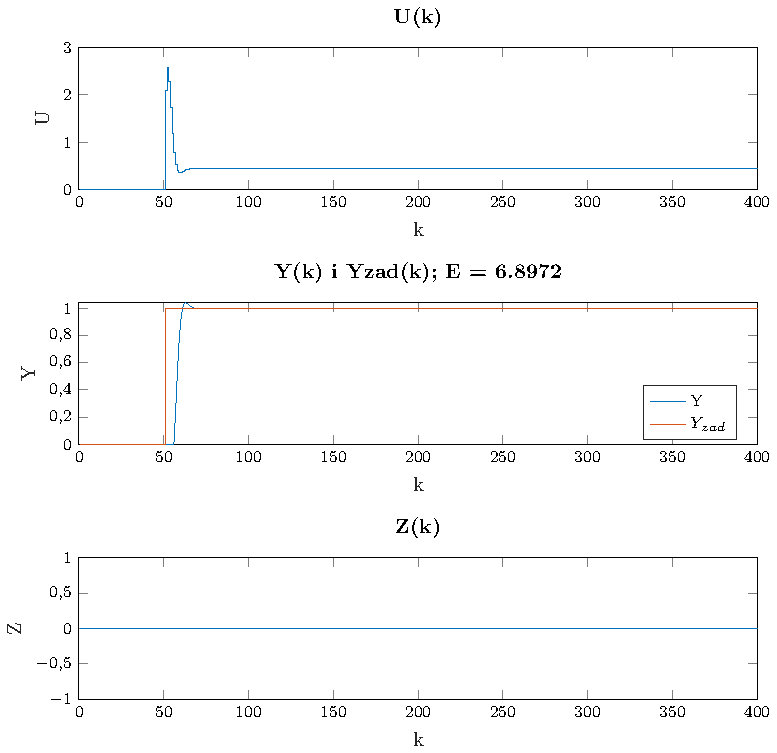
\includegraphics{../../Lab2/PDF_rysunki/Z4_DMCBezZaklocen.pdf}
	\caption{Regulator DMC dla parametrów: ??????}
	\label{dobor_param1}
\end{figure}


\section{Porównanie regulacji DMC z pomiarem zakłócenia oraz bez pomiaru}

\begin{figure}[H]
	\centering
	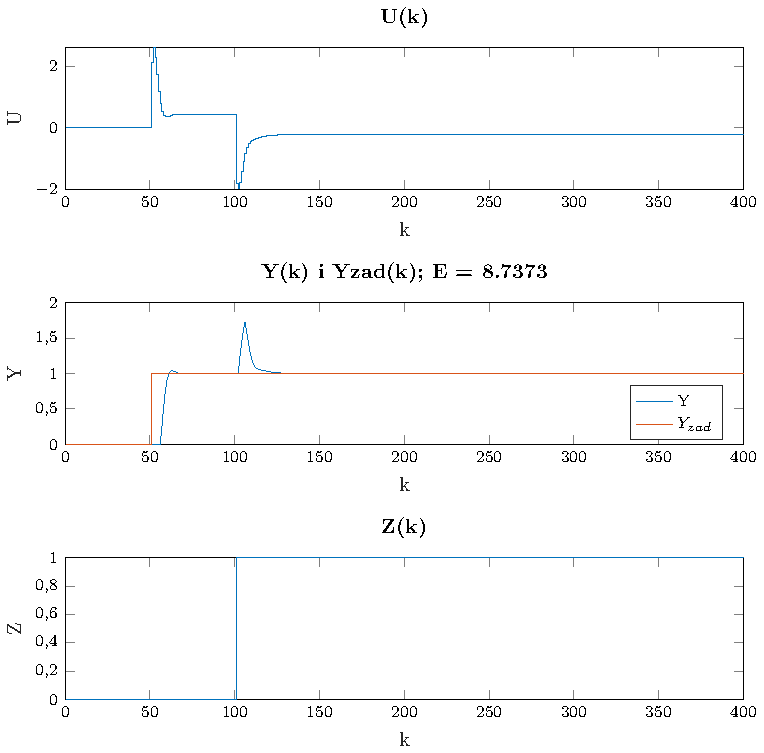
\includegraphics{../../Lab2/PDF_rysunki/Z5_DMCZZakloceniami.pdf}
	\caption{Regulacja DMC z pomiarem zakłócenia : ??????}
	\label{pom_zak}
\end{figure}

\begin{figure}[H]
	\centering
	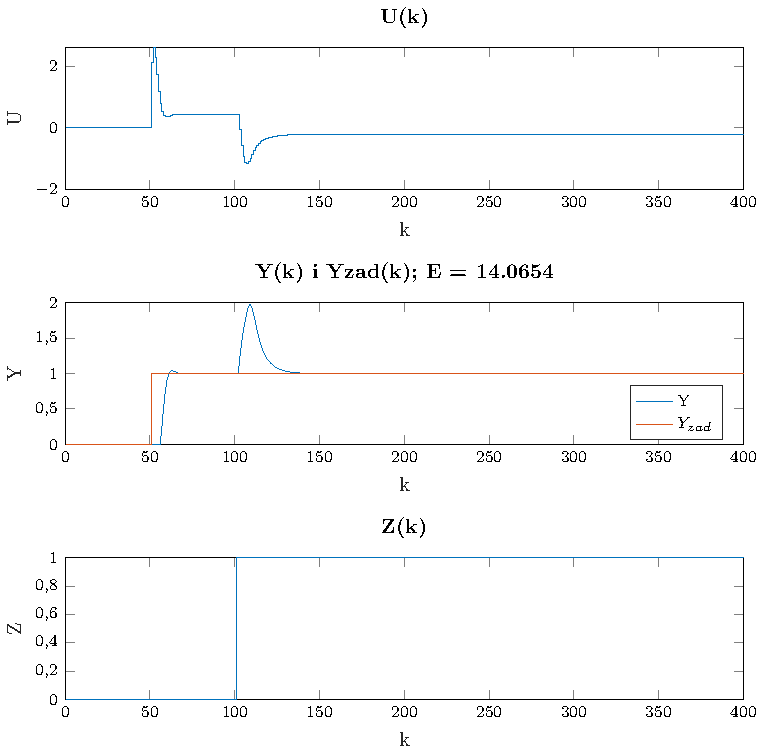
\includegraphics{../../Lab2/PDF_rysunki/Z5_DMCZZakloceniamiBezOdsprz.pdf}
	\caption{Regulacja DMC bez pomiaru zakłócenia: ??????}
	\label{bez_pom_zak}
\end{figure}




\section{Działanie algorytmu DMC z pomiarem zakłóceń przy zakłóceniach sinusoidalnych}


\begin{figure}[H]
	\centering
	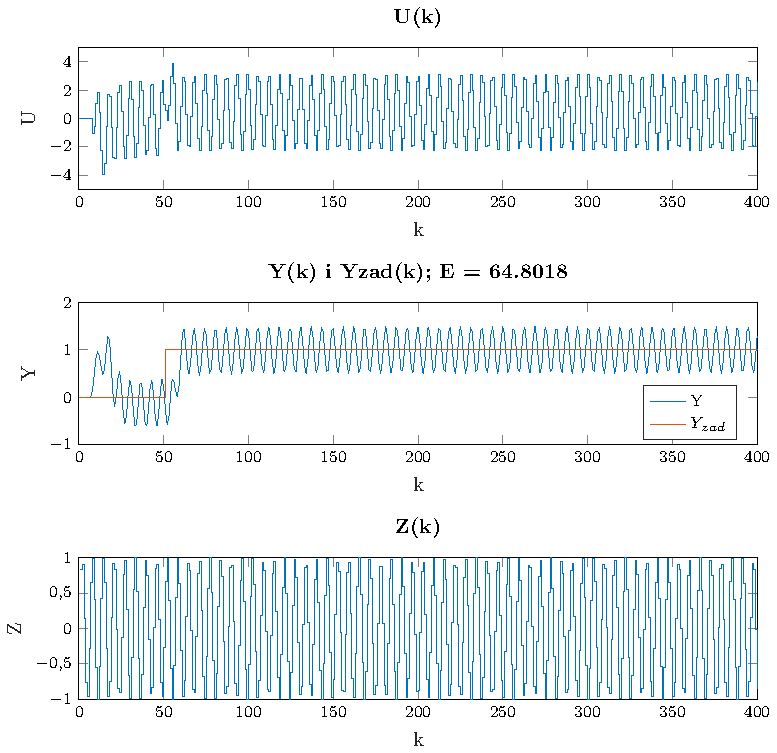
\includegraphics{../../Lab2/PDF_rysunki/Z6_DMCSinZOdsprz.pdf}
	\caption{Regulacja DMC z pomiarem zakłóceń przy zakłóceniach sinusoidalnych}
	\label{sin_z_pom}
\end{figure}

\section{Działanie algorytmu DMC bez pomiaru zakłóceń przy zakłóceniach sinusoidalnych}

\begin{figure}[H]
	\centering
	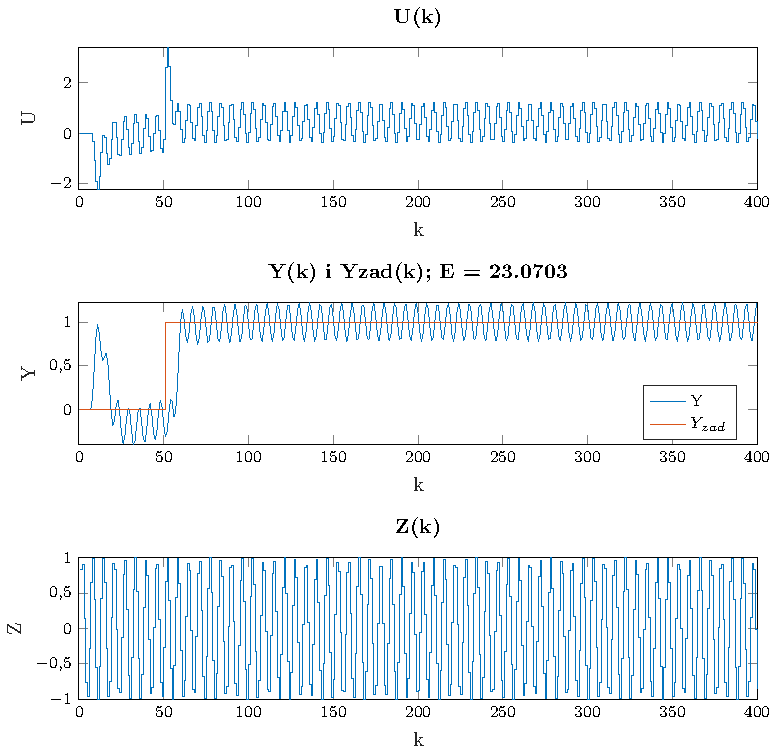
\includegraphics{../../Lab2/PDF_rysunki/Z6_DMCSinBezOdsprz.pdf}
	\caption{Regulacja DMC bez pomiaru zakłóceń przy zakłóceniach sinusoidalnych}
	\label{sin_bez_pom}
\end{figure}

\section{Badanie odporności algorytmu DMC na szum pomiarowy sygnału zakłócenia}

\begin{figure}[H]
	\centering
	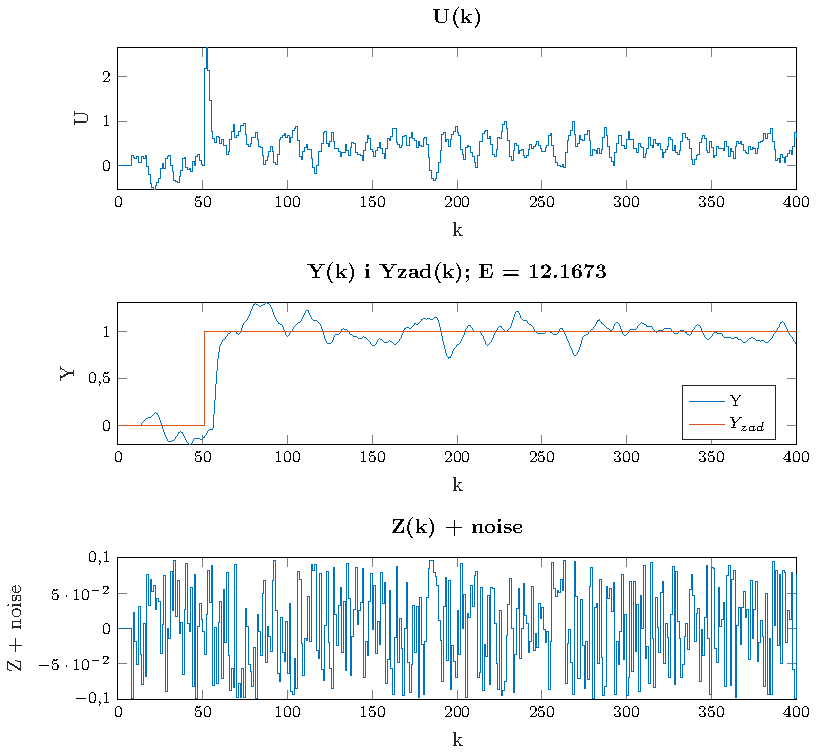
\includegraphics{../../Lab2/PDF_rysunki/Z7_Szum1.pdf}
	\caption{Regulacja DMC z pomiarem zakłóceń z występujacym szumem pomiarowym(1)}
	\label{szum1}
\end{figure}

\begin{figure}[H]
	\centering
	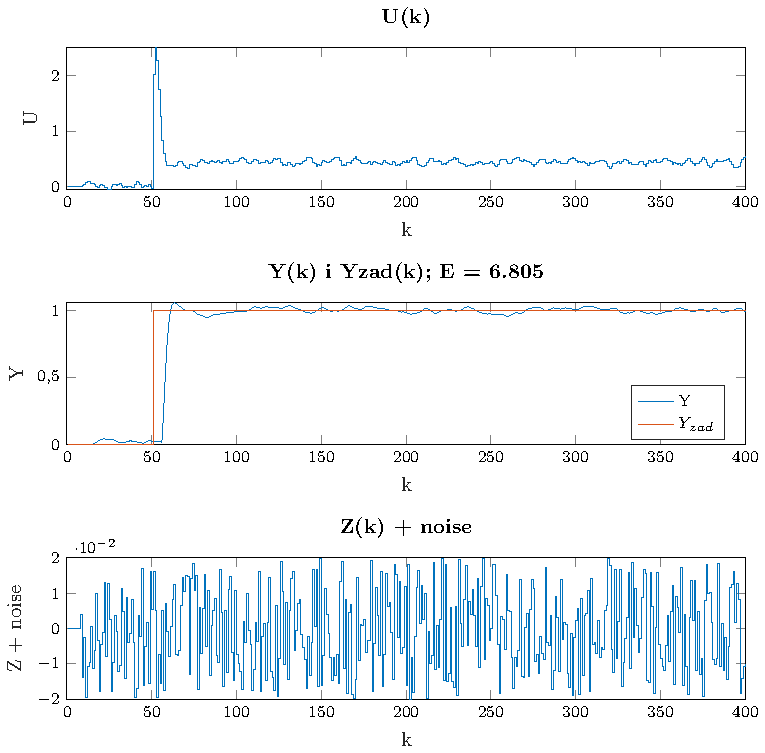
\includegraphics{../../Lab2/PDF_rysunki/Z7_Szum2.pdf}
	\caption{Regulacja DMC z pomiarem zakłóceń z występujacym szumem pomiarowym(2)}
	\label{szum2}
\end{figure}


\begin{figure}[H]
	\centering
	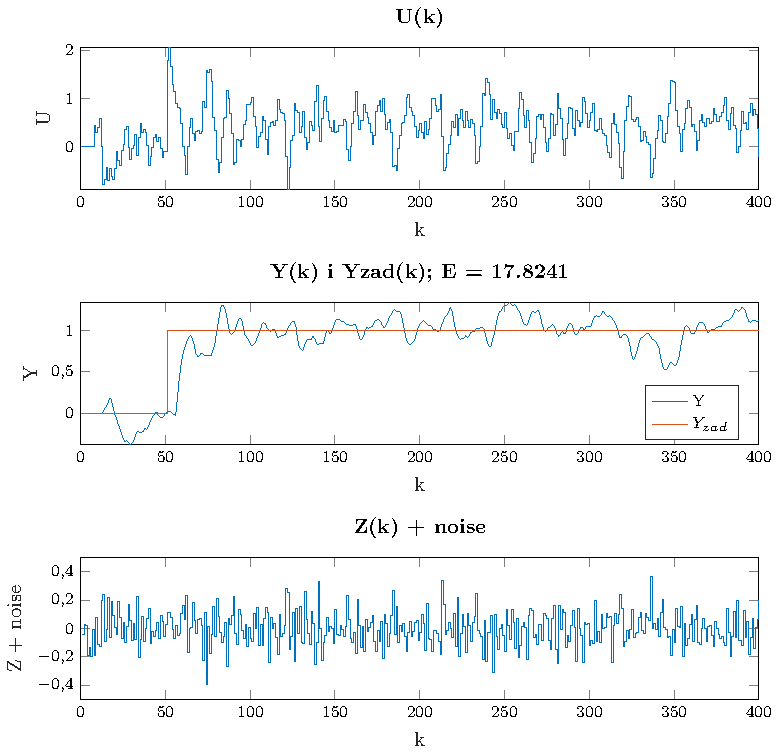
\includegraphics{../../Lab2/PDF_rysunki/Z7_Szum3.pdf}
	\caption{Regulacja DMC z pomiarem zakłóceń z występujacym szumem pomiarowym(3)}
	\label{szum3}
\end{figure}


\begin{figure}[H]
	\centering
	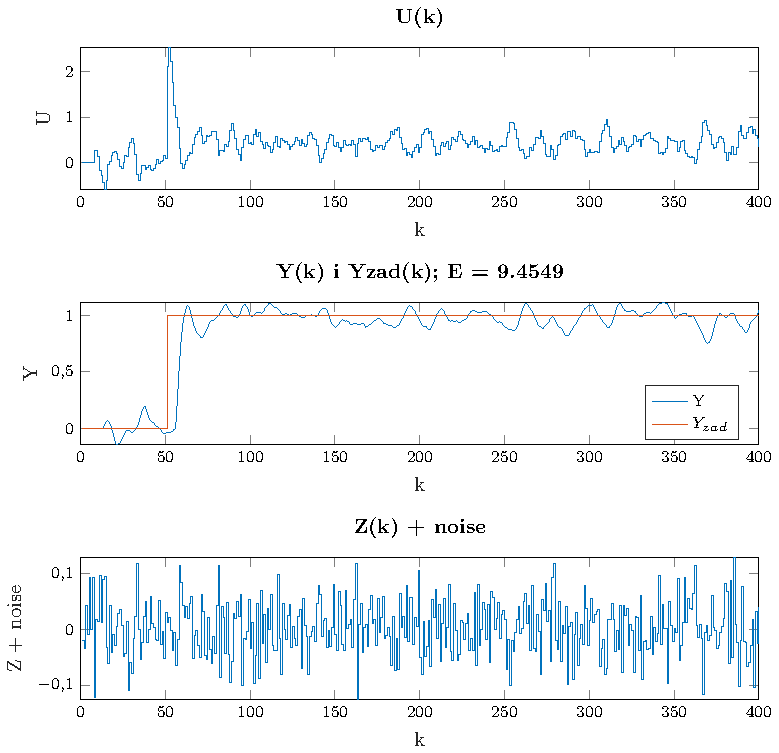
\includegraphics{../../Lab2/PDF_rysunki/Z7_Szum4.pdf}
	\caption{Regulacja DMC z pomiarem zakłóceń z występujacym szumem pomiarowym(4)}
	\label{szum4}
\end{figure}







\begin{comment}
\begin{lstlisting}[style=customlatex,frame=single,] 
roslaunch stero_mobile_init tiago_simple.launch world:=empty
\end{lstlisting}

\section{Cele projektu i laboratoriów}
Celem niniejszego laboratorium było zaprojektowanie, implementacja,
weryfikacja poprawności działania oraz dobór parametrów algorytmów regulacji jednowymiarowego
procesu na grzejąco-chłodzącym stanowisku laboratoryjnym przedstawionym na rys \ref{Stanowisko grzewcze}.


\begin{figure}[h]
	\centering
	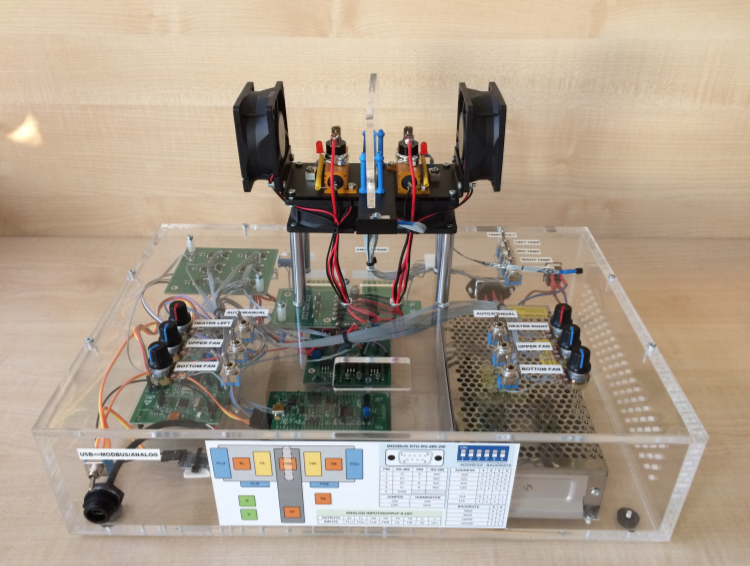
\includegraphics[width=0.7\textwidth]{ ./Rysunki/Stanowisko-grzewcze.png }
	\caption {Stanowisko grzejąco-chłodzące używane w trakcie laboratoriów.}
	\label{Stanowisko grzewcze}
\end{figure}

\begin{figure}[h]
		\centering
		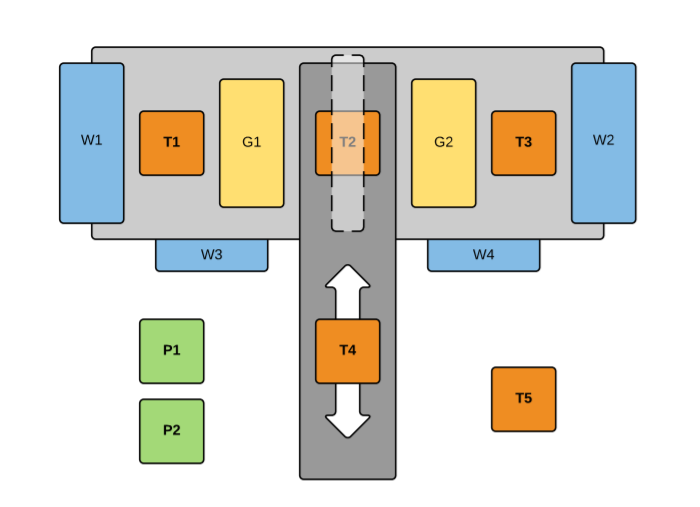
\includegraphics[width=0.7\textwidth]{ ./Rysunki/Stanowisko-grzewcze-schemat.png }
		\caption {
}
		\label{Stanowisko grzewcze, schemat}
\end{figure}

\chapter{Laboratorium}

\section{Przebieg laboratorium}
Rozpoczynając pracę na stanowisku laboratoryjnym należało ustawić moc wentylatora W1
na 50\%. Wentylator ten był traktowany jako cecha otoczenia. Dodatkowo sprawiał on, że temperatura grzałki
opadała szybciej, co było szczególnie przydatne pomiędzy doświadczeniami.

W ramach laboratorium należało wykonać 5 zadań.

\begin{enumerate}
	\label{Lista-zadan}
  \item Odczytać wartość pomiaru temperatury dla termometru T1 dla mocy 26 \% grzałki G1.
  \item Wyznaczyć odpowiedź skokową procesu dla trzech różych wartości G1.
  \item Wybrać jedną z odpowiedzi skokowych, przekształcić ją i wykorzystać w algorytmie DMC. 
  \item Zaimplementować algorytm PID i DMC do regulacji procesu stanowiska w języku MATLAB.
  \item Dobrać nastawy algorytmu PID oraz parametry algorytmu DMC metodą eksperymentalną.
\end{enumerate}

\section{Punkt pracy stanowiska}
W pierwszej kolejności sprawdzono możliwość sterowania i pomiaru w komunikacji ze stanowiskiem.
Następnie  odczytać wartość temperatury termometru T1 w wyznaczonym punkcie pracy G1=26\%.
Po ustawieniu mocy grzałki i odczekaniu, aż temperatura T1 ustabilizuje się,
odczytana wartość termometru T1 wynosiła \num{31.12} °C. Wykres temperatury na termometrze T1 został przedstawiony na rys. \ref{PunktPracy}.

\begin{figure}[h]
	\centering
	% This file was created by matlab2tikz.
%
%The latest updates can be retrieved from
%  http://www.mathworks.com/matlabcentral/fileexchange/22022-matlab2tikz-matlab2tikz
%where you can also make suggestions and rate matlab2tikz.
%
\definecolor{mycolor1}{rgb}{0.00000,0.44700,0.74100}%
%
\begin{tikzpicture}

\begin{axis}[%
width=4.521in,
height=3.566in,
at={(0.758in,0.481in)},
scale only axis,
xmin=1,
xmax=300,
xlabel style={font=\color{white!15!black}},
xlabel={Czas [s]},
ymin=30,
ymax=34,
ylabel style={font=\color{white!15!black}},
ylabel={$\text{Temperatura [}^\circ\text{C]}$},
axis background/.style={fill=white},
title style={font=\bfseries},
title={Punkt Pracy, G1 = 26}
]
\addplot [color=mycolor1, forget plot]
  table[row sep=crcr]{%
1	31.12\\
2	31.12\\
3	31.12\\
4	31.06\\
5	31.12\\
6	31.12\\
7	31.12\\
8	31.12\\
9	31.12\\
10	31.12\\
11	31.12\\
12	31.12\\
13	31.12\\
14	31.12\\
15	31.12\\
16	31.12\\
17	31.12\\
18	31.12\\
19	31.12\\
20	31.12\\
21	31.12\\
22	31.12\\
23	31.12\\
24	31.18\\
25	31.18\\
26	31.12\\
27	31.18\\
28	31.18\\
29	31.12\\
30	31.12\\
31	31.12\\
32	31.18\\
33	31.12\\
34	31.18\\
35	31.18\\
36	31.18\\
37	31.18\\
38	31.18\\
39	31.18\\
40	31.18\\
41	31.18\\
42	31.18\\
43	31.18\\
44	31.18\\
45	31.18\\
46	31.18\\
47	31.18\\
48	31.18\\
49	31.18\\
50	31.18\\
51	31.18\\
52	31.18\\
53	31.18\\
54	31.18\\
55	31.18\\
56	31.18\\
57	31.18\\
58	31.18\\
59	31.18\\
60	31.18\\
61	31.18\\
62	31.12\\
63	31.12\\
64	31.12\\
65	31.12\\
66	31.18\\
67	31.12\\
68	31.12\\
69	31.12\\
70	31.12\\
71	31.12\\
72	31.12\\
73	31.12\\
74	31.12\\
75	31.18\\
76	31.12\\
77	31.18\\
78	31.12\\
79	31.12\\
80	31.12\\
81	31.12\\
82	31.12\\
83	31.12\\
84	31.12\\
85	31.18\\
86	31.18\\
87	31.18\\
88	31.18\\
89	31.18\\
90	31.18\\
91	31.18\\
92	31.18\\
93	31.18\\
94	31.18\\
95	31.18\\
96	31.18\\
97	31.18\\
98	31.18\\
99	31.18\\
100	31.18\\
101	31.18\\
102	31.18\\
103	31.18\\
104	31.18\\
105	31.18\\
106	31.18\\
107	31.18\\
108	31.18\\
109	31.18\\
110	31.18\\
111	31.18\\
112	31.18\\
113	31.18\\
114	31.18\\
115	31.18\\
116	31.18\\
117	31.18\\
118	31.18\\
119	31.18\\
120	31.18\\
121	31.18\\
122	31.18\\
123	31.18\\
124	31.18\\
125	31.18\\
126	31.18\\
127	31.18\\
128	31.18\\
129	31.18\\
130	31.18\\
131	31.18\\
132	31.18\\
133	31.18\\
134	31.18\\
135	31.18\\
136	31.25\\
137	31.18\\
138	31.18\\
139	31.18\\
140	31.18\\
141	31.18\\
142	31.18\\
143	31.12\\
144	31.18\\
145	31.18\\
146	31.12\\
147	31.18\\
148	31.18\\
149	31.18\\
150	31.18\\
151	31.18\\
152	31.18\\
153	31.18\\
154	31.18\\
155	31.18\\
156	31.18\\
157	31.18\\
158	31.18\\
159	31.18\\
160	31.18\\
161	31.18\\
162	31.18\\
163	31.18\\
164	31.18\\
165	31.18\\
166	31.18\\
167	31.18\\
168	31.18\\
169	31.18\\
170	31.18\\
171	31.12\\
172	31.12\\
173	31.18\\
174	31.12\\
175	31.18\\
176	31.12\\
177	31.18\\
178	31.18\\
179	31.18\\
180	31.18\\
181	31.18\\
182	31.18\\
183	31.18\\
184	31.25\\
185	31.25\\
186	31.25\\
187	31.18\\
188	31.25\\
189	31.18\\
190	31.25\\
191	31.25\\
192	31.18\\
193	31.25\\
194	31.18\\
195	31.18\\
196	31.18\\
197	31.18\\
198	31.18\\
199	31.18\\
200	31.18\\
201	31.18\\
202	31.18\\
203	31.18\\
204	31.18\\
205	31.18\\
206	31.18\\
207	31.18\\
208	31.18\\
209	31.18\\
210	31.18\\
211	31.18\\
212	31.18\\
213	31.18\\
214	31.18\\
215	31.18\\
216	31.18\\
217	31.12\\
218	31.12\\
219	31.12\\
220	31.12\\
221	31.12\\
222	31.12\\
223	31.12\\
224	31.12\\
225	31.12\\
226	31.12\\
227	31.12\\
228	31.12\\
229	31.12\\
230	31.12\\
231	31.12\\
232	31.12\\
233	31.18\\
234	31.18\\
235	31.18\\
236	31.18\\
237	31.18\\
238	31.18\\
239	31.18\\
240	31.18\\
241	31.18\\
242	31.18\\
243	31.18\\
244	31.18\\
245	31.18\\
246	31.12\\
247	31.12\\
248	31.12\\
249	31.12\\
250	31.12\\
251	31.12\\
252	31.12\\
253	31.12\\
254	31.12\\
255	31.12\\
256	31.18\\
257	31.18\\
258	31.18\\
259	31.12\\
260	31.12\\
261	31.12\\
262	31.12\\
263	31.12\\
264	31.12\\
265	31.18\\
266	31.12\\
267	31.12\\
268	31.18\\
269	31.12\\
270	31.12\\
271	31.12\\
272	31.12\\
273	31.12\\
274	31.12\\
275	31.12\\
276	31.12\\
277	31.12\\
278	31.12\\
279	31.12\\
280	31.12\\
281	31.12\\
282	31.18\\
283	31.12\\
284	31.12\\
285	31.12\\
286	31.12\\
287	31.12\\
288	31.18\\
289	31.18\\
290	31.12\\
291	31.12\\
292	31.12\\
293	31.12\\
294	31.12\\
295	31.12\\
296	31.12\\
297	31.12\\
298	31.12\\
299	31.12\\
300	31.12\\
};
\end{axis}

\begin{axis}[%
width=5.833in,
height=4.375in,
at={(0in,0in)},
scale only axis,
xmin=0,
xmax=1,
ymin=0,
ymax=1,
axis line style={draw=none},
ticks=none,
axis x line*=bottom,
axis y line*=left
]
\end{axis}
\end{tikzpicture}%
	\caption{Ustalanie się temperatury dla punktu pracy}
	\label{PunktPracy}
\end{figure}


\section{Odpowiedzi skokowe procesu}
W tej części laboratorium należało przeprowadzić eksperyment dla 3 różnych wartości mocy grzałki G1.
Rozpoczynając eksperyment z punktu pracy G1=26\% wyznaczono odpowiedzi skokowe procesu. Eksperyment był wykokany
dla trzech różnych zmian sygnału sterującego, G1=36\%, G1=46\% oraz G1=56\%.
Wykresy przedstawiające zmiany temperatury przedstawiono na rys. \ref{skoki}.


% \begin{figure}
% \centering
% % This file was created by matlab2tikz.
%
%The latest updates can be retrieved from
%  http://www.mathworks.com/matlabcentral/fileexchange/22022-matlab2tikz-matlab2tikz
%where you can also make suggestions and rate matlab2tikz.
%
\definecolor{mycolor1}{rgb}{0.00000,0.44700,0.74100}%
%
\begin{tikzpicture}

\begin{axis}[%
width=4.521in,
height=3.566in,
at={(0.758in,0.481in)},
scale only axis,
xmin=1,
xmax=300,
xlabel style={font=\color{white!15!black}},
xlabel={Czas [s]},
ymin=30,
ymax=42,
ylabel style={font=\color{white!15!black}},
ylabel={$\text{Temperatura [}^\circ\text{C]}$},
axis background/.style={fill=white},
title style={font=\bfseries},
title={$\text{Skok jednostkowy: G1: 26 -\textgreater{} 36}$}
]
\addplot [color=mycolor1, forget plot]
  table[row sep=crcr]{%
1	31.31\\
2	31.31\\
3	31.31\\
4	31.31\\
5	31.31\\
6	31.31\\
7	31.31\\
8	31.31\\
9	31.25\\
10	31.31\\
11	31.25\\
12	31.25\\
13	31.31\\
14	31.31\\
15	31.31\\
16	31.31\\
17	31.31\\
18	31.37\\
19	31.37\\
20	31.43\\
21	31.43\\
22	31.5\\
23	31.5\\
24	31.56\\
25	31.56\\
26	31.56\\
27	31.62\\
28	31.62\\
29	31.68\\
30	31.68\\
31	31.75\\
32	31.75\\
33	31.81\\
34	31.87\\
35	31.87\\
36	31.93\\
37	31.93\\
38	32\\
39	32\\
40	32\\
41	32.06\\
42	32.06\\
43	32.12\\
44	32.12\\
45	32.12\\
46	32.18\\
47	32.18\\
48	32.25\\
49	32.25\\
50	32.31\\
51	32.31\\
52	32.37\\
53	32.37\\
54	32.37\\
55	32.43\\
56	32.43\\
57	32.5\\
58	32.5\\
59	32.56\\
60	32.56\\
61	32.62\\
62	32.62\\
63	32.62\\
64	32.62\\
65	32.68\\
66	32.68\\
67	32.75\\
68	32.75\\
69	32.75\\
70	32.75\\
71	32.81\\
72	32.87\\
73	32.87\\
74	32.87\\
75	32.87\\
76	32.93\\
77	32.93\\
78	32.93\\
79	32.93\\
80	33\\
81	33\\
82	33\\
83	33.06\\
84	33.06\\
85	33.06\\
86	33.06\\
87	33.12\\
88	33.12\\
89	33.12\\
90	33.12\\
91	33.12\\
92	33.18\\
93	33.18\\
94	33.18\\
95	33.25\\
96	33.25\\
97	33.25\\
98	33.25\\
99	33.25\\
100	33.25\\
101	33.31\\
102	33.31\\
103	33.31\\
104	33.31\\
105	33.31\\
106	33.31\\
107	33.31\\
108	33.31\\
109	33.31\\
110	33.31\\
111	33.31\\
112	33.31\\
113	33.31\\
114	33.31\\
115	33.31\\
116	33.37\\
117	33.37\\
118	33.37\\
119	33.37\\
120	33.43\\
121	33.43\\
122	33.43\\
123	33.5\\
124	33.5\\
125	33.5\\
126	33.5\\
127	33.5\\
128	33.56\\
129	33.56\\
130	33.56\\
131	33.56\\
132	33.56\\
133	33.56\\
134	33.56\\
135	33.56\\
136	33.56\\
137	33.56\\
138	33.62\\
139	33.62\\
140	33.62\\
141	33.62\\
142	33.62\\
143	33.62\\
144	33.62\\
145	33.68\\
146	33.68\\
147	33.68\\
148	33.68\\
149	33.68\\
150	33.68\\
151	33.68\\
152	33.68\\
153	33.68\\
154	33.68\\
155	33.75\\
156	33.75\\
157	33.75\\
158	33.75\\
159	33.75\\
160	33.75\\
161	33.75\\
162	33.75\\
163	33.75\\
164	33.81\\
165	33.81\\
166	33.81\\
167	33.81\\
168	33.81\\
169	33.81\\
170	33.81\\
171	33.81\\
172	33.81\\
173	33.81\\
174	33.81\\
175	33.81\\
176	33.87\\
177	33.87\\
178	33.87\\
179	33.87\\
180	33.93\\
181	33.93\\
182	33.93\\
183	33.93\\
184	33.93\\
185	33.93\\
186	33.93\\
187	33.93\\
188	33.93\\
189	34\\
190	33.93\\
191	33.93\\
192	33.93\\
193	34\\
194	34\\
195	34\\
196	34\\
197	34\\
198	34\\
199	34\\
200	34\\
201	34\\
202	34\\
203	34\\
204	34\\
205	34\\
206	34.06\\
207	34\\
208	34.06\\
209	34.06\\
210	34.06\\
211	34.06\\
212	34.06\\
213	34.06\\
214	34.06\\
215	34\\
216	34\\
217	34\\
218	33.93\\
219	33.93\\
220	33.93\\
221	33.93\\
222	33.93\\
223	33.93\\
224	34\\
225	34\\
226	34\\
227	34\\
228	34\\
229	34\\
230	34.06\\
231	34.06\\
232	34.06\\
233	34.06\\
234	34.06\\
235	34.06\\
236	34.06\\
237	34.06\\
238	34.06\\
239	34.06\\
240	34.06\\
241	34.06\\
242	34.12\\
243	34.12\\
244	34.12\\
245	34.12\\
246	34.06\\
247	34.06\\
248	34.06\\
249	34.06\\
250	34.12\\
251	34.12\\
252	34.12\\
253	34.12\\
254	34.12\\
255	34.12\\
256	34.12\\
257	34.12\\
258	34.12\\
259	34.12\\
260	34.12\\
261	34.12\\
262	34.12\\
263	34.12\\
264	34.18\\
265	34.18\\
266	34.18\\
267	34.18\\
268	34.18\\
269	34.18\\
270	34.18\\
271	34.18\\
272	34.18\\
273	34.18\\
274	34.18\\
275	34.18\\
276	34.18\\
277	34.12\\
278	34.18\\
279	34.18\\
280	34.12\\
281	34.12\\
282	34.12\\
283	34.12\\
284	34.12\\
285	34.12\\
286	34.12\\
287	34.12\\
288	34.12\\
289	34.12\\
290	34.12\\
291	34.12\\
292	34.12\\
293	34.12\\
294	34.12\\
295	34.12\\
296	34.12\\
297	34.12\\
298	34.12\\
299	34.12\\
300	34.18\\
};
\end{axis}

\begin{axis}[%
width=5.833in,
height=4.375in,
at={(0in,0in)},
scale only axis,
xmin=0,
xmax=1,
ymin=0,
ymax=1,
axis line style={draw=none},
ticks=none,
axis x line*=bottom,
axis y line*=left
]
\end{axis}
\end{tikzpicture}%
% \caption{Odpowiedź skokowa procesu dla zmiany sterowania G1 z 26 do 36}
% \label{Skok1}
% \end{figure}

% \begin{figure}
% \centering
% % This file was created by matlab2tikz.
%
%The latest updates can be retrieved from
%  http://www.mathworks.com/matlabcentral/fileexchange/22022-matlab2tikz-matlab2tikz
%where you can also make suggestions and rate matlab2tikz.
%
\definecolor{mycolor1}{rgb}{0.00000,0.44700,0.74100}%
%
\begin{tikzpicture}

\begin{axis}[%
width=4.521in,
height=3.566in,
at={(0.758in,0.481in)},
scale only axis,
xmin=1,
xmax=300,
xlabel style={font=\color{white!15!black}},
xlabel={Czas [s]},
ymin=30,
ymax=42,
ylabel style={font=\color{white!15!black}},
ylabel={$\text{Temperatura [}^\circ\text{C]}$},
axis background/.style={fill=white},
title style={font=\bfseries},
title={$\text{Skok jednostkowy: G1: 26 -\textgreater{} 46}$}
]
\addplot [color=mycolor1, forget plot]
  table[row sep=crcr]{%
1	31.31\\
2	31.31\\
3	31.31\\
4	31.31\\
5	31.31\\
6	31.31\\
7	31.31\\
8	31.31\\
9	31.37\\
10	31.37\\
11	31.37\\
12	31.43\\
13	31.5\\
14	31.5\\
15	31.5\\
16	31.56\\
17	31.62\\
18	31.68\\
19	31.68\\
20	31.81\\
21	31.87\\
22	31.87\\
23	31.93\\
24	32\\
25	32.06\\
26	32.12\\
27	32.18\\
28	32.25\\
29	32.37\\
30	32.37\\
31	32.43\\
32	32.5\\
33	32.56\\
34	32.68\\
35	32.75\\
36	32.81\\
37	32.87\\
38	32.93\\
39	33\\
40	33.06\\
41	33.12\\
42	33.18\\
43	33.25\\
44	33.31\\
45	33.37\\
46	33.43\\
47	33.5\\
48	33.56\\
49	33.62\\
50	33.68\\
51	33.68\\
52	33.75\\
53	33.81\\
54	33.81\\
55	33.87\\
56	33.93\\
57	34\\
58	34\\
59	34.06\\
60	34.12\\
61	34.12\\
62	34.18\\
63	34.25\\
64	34.25\\
65	34.31\\
66	34.37\\
67	34.43\\
68	34.43\\
69	34.5\\
70	34.56\\
71	34.62\\
72	34.62\\
73	34.68\\
74	34.75\\
75	34.81\\
76	34.87\\
77	34.87\\
78	34.93\\
79	34.93\\
80	35\\
81	35.06\\
82	35.06\\
83	35.12\\
84	35.12\\
85	35.18\\
86	35.25\\
87	35.25\\
88	35.31\\
89	35.31\\
90	35.31\\
91	35.37\\
92	35.37\\
93	35.37\\
94	35.37\\
95	35.43\\
96	35.5\\
97	35.5\\
98	35.56\\
99	35.56\\
100	35.56\\
101	35.62\\
102	35.62\\
103	35.62\\
104	35.68\\
105	35.68\\
106	35.68\\
107	35.68\\
108	35.75\\
109	35.75\\
110	35.75\\
111	35.75\\
112	35.81\\
113	35.81\\
114	35.87\\
115	35.93\\
116	35.93\\
117	35.93\\
118	35.93\\
119	35.93\\
120	36\\
121	36\\
122	36\\
123	36.06\\
124	36.06\\
125	36.06\\
126	36.12\\
127	36.12\\
128	36.18\\
129	36.18\\
130	36.18\\
131	36.25\\
132	36.18\\
133	36.25\\
134	36.25\\
135	36.31\\
136	36.31\\
137	36.31\\
138	36.37\\
139	36.37\\
140	36.37\\
141	36.37\\
142	36.37\\
143	36.43\\
144	36.43\\
145	36.43\\
146	36.43\\
147	36.43\\
148	36.43\\
149	36.5\\
150	36.5\\
151	36.5\\
152	36.56\\
153	36.56\\
154	36.56\\
155	36.56\\
156	36.62\\
157	36.62\\
158	36.62\\
159	36.62\\
160	36.62\\
161	36.62\\
162	36.62\\
163	36.62\\
164	36.62\\
165	36.62\\
166	36.62\\
167	36.62\\
168	36.62\\
169	36.68\\
170	36.68\\
171	36.68\\
172	36.68\\
173	36.68\\
174	36.68\\
175	36.68\\
176	36.68\\
177	36.75\\
178	36.75\\
179	36.81\\
180	36.81\\
181	36.81\\
182	36.81\\
183	36.87\\
184	36.87\\
185	36.87\\
186	36.87\\
187	36.87\\
188	36.93\\
189	36.93\\
190	36.93\\
191	36.93\\
192	36.93\\
193	36.93\\
194	37\\
195	37\\
196	37\\
197	37\\
198	37\\
199	37\\
200	37\\
201	37\\
202	37\\
203	37\\
204	37\\
205	37.06\\
206	37.06\\
207	37.06\\
208	37.06\\
209	37.12\\
210	37.06\\
211	37.12\\
212	37.12\\
213	37.12\\
214	37.12\\
215	37.06\\
216	37.12\\
217	37.12\\
218	37.12\\
219	37.12\\
220	37.12\\
221	37.18\\
222	37.18\\
223	37.18\\
224	37.18\\
225	37.18\\
226	37.25\\
227	37.25\\
228	37.25\\
229	37.25\\
230	37.25\\
231	37.31\\
232	37.31\\
233	37.31\\
234	37.31\\
235	37.31\\
236	37.31\\
237	37.37\\
238	37.37\\
239	37.37\\
240	37.37\\
241	37.37\\
242	37.37\\
243	37.43\\
244	37.37\\
245	37.43\\
246	37.43\\
247	37.37\\
248	37.43\\
249	37.43\\
250	37.43\\
251	37.43\\
252	37.43\\
253	37.43\\
254	37.43\\
255	37.37\\
256	37.43\\
257	37.43\\
258	37.43\\
259	37.43\\
260	37.43\\
261	37.43\\
262	37.43\\
263	37.43\\
264	37.43\\
265	37.43\\
266	37.43\\
267	37.43\\
268	37.43\\
269	37.5\\
270	37.43\\
271	37.5\\
272	37.5\\
273	37.5\\
274	37.5\\
275	37.5\\
276	37.5\\
277	37.56\\
278	37.56\\
279	37.56\\
280	37.5\\
281	37.56\\
282	37.56\\
283	37.56\\
284	37.56\\
285	37.56\\
286	37.56\\
287	37.62\\
288	37.62\\
289	37.62\\
290	37.62\\
291	37.62\\
292	37.62\\
293	37.62\\
294	37.62\\
295	37.62\\
296	37.62\\
297	37.62\\
298	37.62\\
299	37.62\\
300	37.62\\
};
\end{axis}

\begin{axis}[%
width=5.833in,
height=4.375in,
at={(0in,0in)},
scale only axis,
xmin=0,
xmax=1,
ymin=0,
ymax=1,
axis line style={draw=none},
ticks=none,
axis x line*=bottom,
axis y line*=left
]
\end{axis}
\end{tikzpicture}%
% \caption{Odpowiedź skokowa procesu dla zmiany sterowania G1 z 26 do 46}
% \label{Skok2}
% \end{figure}

\begin{figure}[h]
\centering
% This file was created by matlab2tikz.
%
\definecolor{mycolor1}{rgb}{0.00000,0.44700,0.74100}%
\definecolor{mycolor2}{rgb}{0.85000,0.32500,0.09800}%
\definecolor{mycolor3}{rgb}{0.92900,0.69400,0.12500}%
%
\begin{tikzpicture}

\begin{axis}[%
width=4.521in,
height=3.566in,
at={(0.758in,0.481in)},
scale only axis,
xmin=0,
xmax=300,
xlabel style={font=\color{white!15!black}},
xlabel={Czas [s]},
ymin=31,
ymax=41,
ylabel style={font=\color{white!15!black}},
ylabel={$\text{Temperatura [}^\circ\text{C]}$},
axis background/.style={fill=white},
title style={font=\bfseries},
title={$\text{Odpowiedzi skokowe z punktu pracy (G1 = 26\%, T1 = 31,12}^\circ\text{C)}$},
axis x line*=bottom,
axis y line*=left,
legend style={at={(0.03,0.97)}, anchor=north west, legend cell align=left, align=left, draw=white!15!black}
]
\addplot [color=mycolor1]
  table[row sep=crcr]{%
1	31.31\\
2	31.31\\
3	31.31\\
4	31.31\\
5	31.31\\
6	31.31\\
7	31.31\\
8	31.31\\
9	31.25\\
10	31.31\\
11	31.25\\
12	31.25\\
13	31.31\\
14	31.31\\
15	31.31\\
16	31.31\\
17	31.31\\
18	31.37\\
19	31.37\\
20	31.43\\
21	31.43\\
22	31.5\\
23	31.5\\
24	31.56\\
25	31.56\\
26	31.56\\
27	31.62\\
28	31.62\\
29	31.68\\
30	31.68\\
31	31.75\\
32	31.75\\
33	31.81\\
34	31.87\\
35	31.87\\
36	31.93\\
37	31.93\\
38	32\\
39	32\\
40	32\\
41	32.06\\
42	32.06\\
43	32.12\\
44	32.12\\
45	32.12\\
46	32.18\\
47	32.18\\
48	32.25\\
49	32.25\\
50	32.31\\
51	32.31\\
52	32.37\\
53	32.37\\
54	32.37\\
55	32.43\\
56	32.43\\
57	32.5\\
58	32.5\\
59	32.56\\
60	32.56\\
61	32.62\\
62	32.62\\
63	32.62\\
64	32.62\\
65	32.68\\
66	32.68\\
67	32.75\\
68	32.75\\
69	32.75\\
70	32.75\\
71	32.81\\
72	32.87\\
73	32.87\\
74	32.87\\
75	32.87\\
76	32.93\\
77	32.93\\
78	32.93\\
79	32.93\\
80	33\\
81	33\\
82	33\\
83	33.06\\
84	33.06\\
85	33.06\\
86	33.06\\
87	33.12\\
88	33.12\\
89	33.12\\
90	33.12\\
91	33.12\\
92	33.18\\
93	33.18\\
94	33.18\\
95	33.25\\
96	33.25\\
97	33.25\\
98	33.25\\
99	33.25\\
100	33.25\\
101	33.31\\
102	33.31\\
103	33.31\\
104	33.31\\
105	33.31\\
106	33.31\\
107	33.31\\
108	33.31\\
109	33.31\\
110	33.31\\
111	33.31\\
112	33.31\\
113	33.31\\
114	33.31\\
115	33.31\\
116	33.37\\
117	33.37\\
118	33.37\\
119	33.37\\
120	33.43\\
121	33.43\\
122	33.43\\
123	33.5\\
124	33.5\\
125	33.5\\
126	33.5\\
127	33.5\\
128	33.56\\
129	33.56\\
130	33.56\\
131	33.56\\
132	33.56\\
133	33.56\\
134	33.56\\
135	33.56\\
136	33.56\\
137	33.56\\
138	33.62\\
139	33.62\\
140	33.62\\
141	33.62\\
142	33.62\\
143	33.62\\
144	33.62\\
145	33.68\\
146	33.68\\
147	33.68\\
148	33.68\\
149	33.68\\
150	33.68\\
151	33.68\\
152	33.68\\
153	33.68\\
154	33.68\\
155	33.75\\
156	33.75\\
157	33.75\\
158	33.75\\
159	33.75\\
160	33.75\\
161	33.75\\
162	33.75\\
163	33.75\\
164	33.81\\
165	33.81\\
166	33.81\\
167	33.81\\
168	33.81\\
169	33.81\\
170	33.81\\
171	33.81\\
172	33.81\\
173	33.81\\
174	33.81\\
175	33.81\\
176	33.87\\
177	33.87\\
178	33.87\\
179	33.87\\
180	33.93\\
181	33.93\\
182	33.93\\
183	33.93\\
184	33.93\\
185	33.93\\
186	33.93\\
187	33.93\\
188	33.93\\
189	34\\
190	33.93\\
191	33.93\\
192	33.93\\
193	34\\
194	34\\
195	34\\
196	34\\
197	34\\
198	34\\
199	34\\
200	34\\
201	34\\
202	34\\
203	34\\
204	34\\
205	34\\
206	34.06\\
207	34\\
208	34.06\\
209	34.06\\
210	34.06\\
211	34.06\\
212	34.06\\
213	34.06\\
214	34.06\\
215	34\\
216	34\\
217	34\\
218	33.93\\
219	33.93\\
220	33.93\\
221	33.93\\
222	33.93\\
223	33.93\\
224	34\\
225	34\\
226	34\\
227	34\\
228	34\\
229	34\\
230	34.06\\
231	34.06\\
232	34.06\\
233	34.06\\
234	34.06\\
235	34.06\\
236	34.06\\
237	34.06\\
238	34.06\\
239	34.06\\
240	34.06\\
241	34.06\\
242	34.12\\
243	34.12\\
244	34.12\\
245	34.12\\
246	34.06\\
247	34.06\\
248	34.06\\
249	34.06\\
250	34.12\\
251	34.12\\
252	34.12\\
253	34.12\\
254	34.12\\
255	34.12\\
256	34.12\\
257	34.12\\
258	34.12\\
259	34.12\\
260	34.12\\
261	34.12\\
262	34.12\\
263	34.12\\
264	34.18\\
265	34.18\\
266	34.18\\
267	34.18\\
268	34.18\\
269	34.18\\
270	34.18\\
271	34.18\\
272	34.18\\
273	34.18\\
274	34.18\\
275	34.18\\
276	34.18\\
277	34.12\\
278	34.18\\
279	34.18\\
280	34.12\\
281	34.12\\
282	34.12\\
283	34.12\\
284	34.12\\
285	34.12\\
286	34.12\\
287	34.12\\
288	34.12\\
289	34.12\\
290	34.12\\
291	34.12\\
292	34.12\\
293	34.12\\
294	34.12\\
295	34.12\\
296	34.12\\
297	34.12\\
298	34.12\\
299	34.12\\
300	34.18\\
};
\addlegendentry{dla G1 = 36\%}

\addplot [color=mycolor2]
  table[row sep=crcr]{%
1	31.31\\
2	31.31\\
3	31.31\\
4	31.31\\
5	31.31\\
6	31.31\\
7	31.31\\
8	31.31\\
9	31.37\\
10	31.37\\
11	31.37\\
12	31.43\\
13	31.5\\
14	31.5\\
15	31.5\\
16	31.56\\
17	31.62\\
18	31.68\\
19	31.68\\
20	31.81\\
21	31.87\\
22	31.87\\
23	31.93\\
24	32\\
25	32.06\\
26	32.12\\
27	32.18\\
28	32.25\\
29	32.37\\
30	32.37\\
31	32.43\\
32	32.5\\
33	32.56\\
34	32.68\\
35	32.75\\
36	32.81\\
37	32.87\\
38	32.93\\
39	33\\
40	33.06\\
41	33.12\\
42	33.18\\
43	33.25\\
44	33.31\\
45	33.37\\
46	33.43\\
47	33.5\\
48	33.56\\
49	33.62\\
50	33.68\\
51	33.68\\
52	33.75\\
53	33.81\\
54	33.81\\
55	33.87\\
56	33.93\\
57	34\\
58	34\\
59	34.06\\
60	34.12\\
61	34.12\\
62	34.18\\
63	34.25\\
64	34.25\\
65	34.31\\
66	34.37\\
67	34.43\\
68	34.43\\
69	34.5\\
70	34.56\\
71	34.62\\
72	34.62\\
73	34.68\\
74	34.75\\
75	34.81\\
76	34.87\\
77	34.87\\
78	34.93\\
79	34.93\\
80	35\\
81	35.06\\
82	35.06\\
83	35.12\\
84	35.12\\
85	35.18\\
86	35.25\\
87	35.25\\
88	35.31\\
89	35.31\\
90	35.31\\
91	35.37\\
92	35.37\\
93	35.37\\
94	35.37\\
95	35.43\\
96	35.5\\
97	35.5\\
98	35.56\\
99	35.56\\
100	35.56\\
101	35.62\\
102	35.62\\
103	35.62\\
104	35.68\\
105	35.68\\
106	35.68\\
107	35.68\\
108	35.75\\
109	35.75\\
110	35.75\\
111	35.75\\
112	35.81\\
113	35.81\\
114	35.87\\
115	35.93\\
116	35.93\\
117	35.93\\
118	35.93\\
119	35.93\\
120	36\\
121	36\\
122	36\\
123	36.06\\
124	36.06\\
125	36.06\\
126	36.12\\
127	36.12\\
128	36.18\\
129	36.18\\
130	36.18\\
131	36.25\\
132	36.18\\
133	36.25\\
134	36.25\\
135	36.31\\
136	36.31\\
137	36.31\\
138	36.37\\
139	36.37\\
140	36.37\\
141	36.37\\
142	36.37\\
143	36.43\\
144	36.43\\
145	36.43\\
146	36.43\\
147	36.43\\
148	36.43\\
149	36.5\\
150	36.5\\
151	36.5\\
152	36.56\\
153	36.56\\
154	36.56\\
155	36.56\\
156	36.62\\
157	36.62\\
158	36.62\\
159	36.62\\
160	36.62\\
161	36.62\\
162	36.62\\
163	36.62\\
164	36.62\\
165	36.62\\
166	36.62\\
167	36.62\\
168	36.62\\
169	36.68\\
170	36.68\\
171	36.68\\
172	36.68\\
173	36.68\\
174	36.68\\
175	36.68\\
176	36.68\\
177	36.75\\
178	36.75\\
179	36.81\\
180	36.81\\
181	36.81\\
182	36.81\\
183	36.87\\
184	36.87\\
185	36.87\\
186	36.87\\
187	36.87\\
188	36.93\\
189	36.93\\
190	36.93\\
191	36.93\\
192	36.93\\
193	36.93\\
194	37\\
195	37\\
196	37\\
197	37\\
198	37\\
199	37\\
200	37\\
201	37\\
202	37\\
203	37\\
204	37\\
205	37.06\\
206	37.06\\
207	37.06\\
208	37.06\\
209	37.12\\
210	37.06\\
211	37.12\\
212	37.12\\
213	37.12\\
214	37.12\\
215	37.06\\
216	37.12\\
217	37.12\\
218	37.12\\
219	37.12\\
220	37.12\\
221	37.18\\
222	37.18\\
223	37.18\\
224	37.18\\
225	37.18\\
226	37.25\\
227	37.25\\
228	37.25\\
229	37.25\\
230	37.25\\
231	37.31\\
232	37.31\\
233	37.31\\
234	37.31\\
235	37.31\\
236	37.31\\
237	37.37\\
238	37.37\\
239	37.37\\
240	37.37\\
241	37.37\\
242	37.37\\
243	37.43\\
244	37.37\\
245	37.43\\
246	37.43\\
247	37.37\\
248	37.43\\
249	37.43\\
250	37.43\\
251	37.43\\
252	37.43\\
253	37.43\\
254	37.43\\
255	37.37\\
256	37.43\\
257	37.43\\
258	37.43\\
259	37.43\\
260	37.43\\
261	37.43\\
262	37.43\\
263	37.43\\
264	37.43\\
265	37.43\\
266	37.43\\
267	37.43\\
268	37.43\\
269	37.5\\
270	37.43\\
271	37.5\\
272	37.5\\
273	37.5\\
274	37.5\\
275	37.5\\
276	37.5\\
277	37.56\\
278	37.56\\
279	37.56\\
280	37.5\\
281	37.56\\
282	37.56\\
283	37.56\\
284	37.56\\
285	37.56\\
286	37.56\\
287	37.62\\
288	37.62\\
289	37.62\\
290	37.62\\
291	37.62\\
292	37.62\\
293	37.62\\
294	37.62\\
295	37.62\\
296	37.62\\
297	37.62\\
298	37.62\\
299	37.62\\
300	37.62\\
};
\addlegendentry{dla G1 = 46\%}

\addplot [color=mycolor3]
  table[row sep=crcr]{%
1	31.18\\
2	31.18\\
3	31.18\\
4	31.18\\
5	31.18\\
6	31.18\\
7	31.18\\
8	31.25\\
9	31.25\\
10	31.31\\
11	31.31\\
12	31.37\\
13	31.43\\
14	31.5\\
15	31.5\\
16	31.62\\
17	31.68\\
18	31.75\\
19	31.81\\
20	31.93\\
21	32\\
22	32.06\\
23	32.18\\
24	32.31\\
25	32.37\\
26	32.43\\
27	32.56\\
28	32.68\\
29	32.75\\
30	32.87\\
31	32.93\\
32	33.06\\
33	33.12\\
34	33.25\\
35	33.31\\
36	33.43\\
37	33.56\\
38	33.62\\
39	33.75\\
40	33.87\\
41	33.93\\
42	34.06\\
43	34.12\\
44	34.25\\
45	34.31\\
46	34.43\\
47	34.5\\
48	34.62\\
49	34.68\\
50	34.75\\
51	34.87\\
52	34.93\\
53	35\\
54	35.12\\
55	35.18\\
56	35.25\\
57	35.31\\
58	35.37\\
59	35.43\\
60	35.56\\
61	35.62\\
62	35.68\\
63	35.68\\
64	35.81\\
65	35.81\\
66	35.87\\
67	35.93\\
68	36\\
69	36.06\\
70	36.12\\
71	36.18\\
72	36.31\\
73	36.31\\
74	36.37\\
75	36.43\\
76	36.5\\
77	36.56\\
78	36.62\\
79	36.68\\
80	36.68\\
81	36.75\\
82	36.81\\
83	36.87\\
84	36.87\\
85	36.93\\
86	37\\
87	37.06\\
88	37.12\\
89	37.18\\
90	37.25\\
91	37.25\\
92	37.37\\
93	37.37\\
94	37.43\\
95	37.5\\
96	37.5\\
97	37.56\\
98	37.56\\
99	37.62\\
100	37.68\\
101	37.75\\
102	37.75\\
103	37.81\\
104	37.81\\
105	37.87\\
106	37.93\\
107	37.93\\
108	38\\
109	38\\
110	38.06\\
111	38.06\\
112	38.12\\
113	38.18\\
114	38.18\\
115	38.18\\
116	38.25\\
117	38.25\\
118	38.31\\
119	38.37\\
120	38.37\\
121	38.43\\
122	38.43\\
123	38.5\\
124	38.5\\
125	38.5\\
126	38.56\\
127	38.56\\
128	38.56\\
129	38.62\\
130	38.62\\
131	38.62\\
132	38.62\\
133	38.62\\
134	38.68\\
135	38.68\\
136	38.68\\
137	38.75\\
138	38.75\\
139	38.81\\
140	38.81\\
141	38.87\\
142	38.87\\
143	38.93\\
144	38.93\\
145	39\\
146	39\\
147	38.93\\
148	39\\
149	39\\
150	39\\
151	39\\
152	39\\
153	39.06\\
154	39.06\\
155	39.06\\
156	39.12\\
157	39.12\\
158	39.18\\
159	39.18\\
160	39.25\\
161	39.25\\
162	39.25\\
163	39.31\\
164	39.31\\
165	39.37\\
166	39.37\\
167	39.37\\
168	39.37\\
169	39.43\\
170	39.43\\
171	39.5\\
172	39.5\\
173	39.5\\
174	39.5\\
175	39.5\\
176	39.56\\
177	39.56\\
178	39.56\\
179	39.56\\
180	39.56\\
181	39.62\\
182	39.62\\
183	39.62\\
184	39.62\\
185	39.62\\
186	39.62\\
187	39.68\\
188	39.68\\
189	39.68\\
190	39.75\\
191	39.75\\
192	39.75\\
193	39.75\\
194	39.75\\
195	39.81\\
196	39.81\\
197	39.81\\
198	39.87\\
199	39.87\\
200	39.87\\
201	39.87\\
202	39.87\\
203	39.93\\
204	39.93\\
205	39.93\\
206	39.93\\
207	39.93\\
208	39.93\\
209	39.93\\
210	39.93\\
211	39.93\\
212	39.93\\
213	39.93\\
214	39.93\\
215	40\\
216	40\\
217	40.06\\
218	40.06\\
219	40.06\\
220	40.12\\
221	40.06\\
222	40.12\\
223	40.18\\
224	40.12\\
225	40.18\\
226	40.18\\
227	40.18\\
228	40.18\\
229	40.18\\
230	40.18\\
231	40.18\\
232	40.18\\
233	40.18\\
234	40.18\\
235	40.18\\
236	40.25\\
237	40.25\\
238	40.25\\
239	40.25\\
240	40.25\\
241	40.31\\
242	40.31\\
243	40.31\\
244	40.31\\
245	40.31\\
246	40.31\\
247	40.37\\
248	40.37\\
249	40.37\\
250	40.43\\
251	40.43\\
252	40.43\\
253	40.43\\
254	40.43\\
255	40.43\\
256	40.43\\
257	40.5\\
258	40.43\\
259	40.43\\
260	40.43\\
261	40.5\\
262	40.5\\
263	40.5\\
264	40.5\\
265	40.5\\
266	40.5\\
267	40.5\\
268	40.5\\
269	40.5\\
270	40.5\\
271	40.5\\
272	40.5\\
273	40.5\\
274	40.5\\
275	40.5\\
276	40.5\\
277	40.5\\
278	40.5\\
279	40.5\\
280	40.56\\
281	40.56\\
282	40.56\\
283	40.56\\
284	40.56\\
285	40.62\\
286	40.62\\
287	40.62\\
288	40.68\\
289	40.68\\
290	40.68\\
291	40.68\\
292	40.68\\
293	40.68\\
294	40.75\\
295	40.75\\
296	40.75\\
297	40.75\\
298	40.75\\
299	40.75\\
300	40.75\\
};
\addlegendentry{dla G1 = 56\%}

\end{axis}
\end{tikzpicture}%
\caption{Odpowiedź skokowa procesu}
\label{skoki}
\end{figure}

Patrząc na wykres odpowiedzi skokowych możemy zauważyć, że proces jest w przybliżeniu liniowy. Na rys. \ref{charakterystyka-statyczna} została przedstawiona charakterystyka statyczna procesu.

\begin{figure}[h]
	\centering
	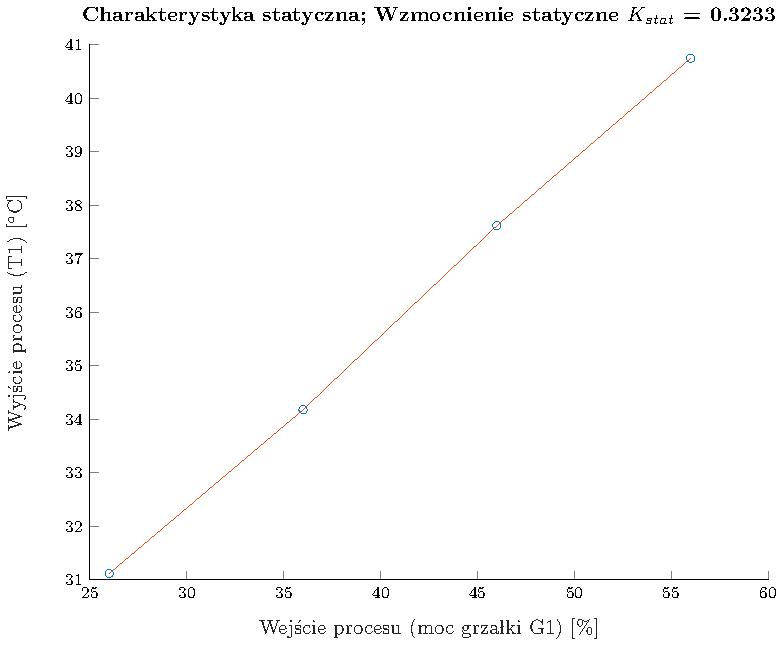
\includegraphics{../TikZ_rysunki/charakterystyka_stat.pdf}
	\caption{Charkterystyk statyczna procesu grzejąco-chłodzącego}
	\label{charakterystyka-statyczna}
\end{figure}


\section{Odpowiedź skokowa w algorytmie DMC}
Wykonanie tego zadania polegało na przekształceniu jednej z odpowiedzi
skokowych, tak aby otrzymać odpowiedź skokową używaną w algorymie DMC.
W tym celu wybrano drugą odpowiedź skokową, tj. skok G1 z mocy 26\% do mocy 46\%.
Do przekształcenia zebranej odpowiedzi skokowej, na taką nadającą się do algorytmu DMC wykorzystano program \emph{SkokDMC.m}.
Program ten wylicza potrzebną odpowiedź skokową przy użyciu prostego wzoru.
\begin{equation}
	S(i)= \frac{Y(i) - Y_{\mathrm{pp}}}{U_{\mathrm{skok}} - U_{\mathrm{pp}}}
\end{equation}
gdzie:
\begin{itemize}
  \item $S(i)$ - odpowiedź skokowa potrzebna do algorytmu DMC,
	\item $Y(i)$ - odpowiedź skokowa przed przekształceniem,
	\item $Y_{\mathrm{pp}}$ - wartość wyjścia w chwili k=0 (tutaj $Y_{\mathrm{pp}}$  = \num{31.12} ),
	\item $U_{\mathrm{skok}}$ - wartość sterowanie w chwili k=0 i później (tutaj $U_{\mathrm{skok}} = 46$),
	\item $U_{\mathrm{pp}}$ - wartośc sterowania przed chwilą k=0 (tutaj $U_{\mathrm{pp}} = 26$)
\end{itemize}
W ten sposób przekształcona odpowiedź skokowa została zapisana do pliku \emph{dane1.mat}
i wykorzystana w dalszych częściach laboratoriów.

Poza przekształceniem odpowiedzi skokowej należało ją jeszcze przybliżyć używając w tym celu członu inercyjnego
drugiego rzędu z opóźnieniem.

\begin{equation}
	G(s)= \frac{K}{(sT_1 + 1)(sT_2 + 1)}e^{-T_{\mathrm{d}}s}
\end{equation}
Po dyskretyzacji danej transmitancji otrzymujemy:

\begin{equation}
	G(z)= \frac{b_1z^{-1} + b_2z^{-2}}{1 + a_1z^{-1} + a_2z^{-2}}z^{-T_{\mathrm{d}}}
\end{equation}

gdzie
\begin{equation}
\begin{split}
	& a_1 = -\alpha_1 - \alpha_2 \\
	& a_2 = \alpha_1\alpha_2 \\
	& \alpha_1 = e^{-\frac{1}{T_1}} \\
	& \alpha_2 = e^{-\frac{1}{T_2}} \\
	& b_1 = \frac{K}{T_1 - T_2}[T_1(1-\alpha_1) - T_2(1-\alpha_2)] \\
	& b_2 = \frac{K}{T_1 - T_2}[\alpha_1T_2(1-\alpha_2) - \alpha_2T_1(1-\alpha_1)]
\end{split}
\end{equation}

Z wykresu odpowiedzi skokowej procesu zostało odczytane opóźnienie. W naszym przypadku $T_{\mathrm{d}} = 9$.
Aby wyznaczyć wartości pozostałych współczynników użyto dostępnej w matlabie funkcji ga, która minimalizuje
wartość zadanej funkcji z wykorzystaniem algorytmu generycznego. Funkcja minimalizowana to funkcja wyliczająca sumę kwadratów błędów
pomiędzy odpowiedzią skokową, a transmitancją przybliżającą.

\lstinputlisting{../Programy/AproksSkokDMC.m}

Następnie używając skryptu \emph{Optymalizacja.m} zostały wyznaczone pozostałe parametry transmitancji przybliżającej odpowiedź skokową.
Ostateczne wartości parametrów to:

\begin{equation}
	\begin{split}
		& K = 0.330938\\
		& T_1 = 0.000907 \\
		& T_2 = 82.104622 \\
		& T_{\mathrm{d}} = 9 \\
	\end{split}
\end{equation}

\begin{figure}[h]
	\centering
	% This file was created by matlab2tikz.
%
%The latest updates can be retrieved from
%  http://www.mathworks.com/matlabcentral/fileexchange/22022-matlab2tikz-matlab2tikz
%where you can also make suggestions and rate matlab2tikz.
%
\definecolor{mycolor1}{rgb}{0.00000,0.44700,0.74100}%
\definecolor{mycolor2}{rgb}{0.85000,0.32500,0.09800}%
%
\begin{tikzpicture}

\begin{axis}[%
width=4.521in,
height=3.566in,
at={(0.758in,0.481in)},
scale only axis,
xmin=0,
xmax=300,
xlabel style={font=\color{white!15!black}},
xlabel={k},
ymin=0,
ymax=0.35,
ylabel style={font=\color{white!15!black}},
ylabel={$\text{S}_\text{k}$},
axis background/.style={fill=white},
title style={font=\bfseries},
title={Aproksymacja odpowiedzi skokowej; E = 0.0047674}
]
\addplot [color=mycolor1, forget plot]
  table[row sep=crcr]{%
1	0.00949999999999989\\
2	0.00949999999999989\\
3	0.00949999999999989\\
4	0.00949999999999989\\
5	0.00949999999999989\\
6	0.00949999999999989\\
7	0.00949999999999989\\
8	0.00949999999999989\\
9	0.0125\\
10	0.0125\\
11	0.0125\\
12	0.0154999999999999\\
13	0.019\\
14	0.019\\
15	0.019\\
16	0.0219999999999999\\
17	0.025\\
18	0.0279999999999999\\
19	0.0279999999999999\\
20	0.0344999999999999\\
21	0.0375\\
22	0.0375\\
23	0.0404999999999999\\
24	0.0439999999999999\\
25	0.0470000000000001\\
26	0.0499999999999998\\
27	0.0529999999999999\\
28	0.0565\\
29	0.0624999999999998\\
30	0.0624999999999998\\
31	0.0654999999999999\\
32	0.069\\
33	0.0720000000000001\\
34	0.0779999999999999\\
35	0.0814999999999999\\
36	0.0845000000000001\\
37	0.0874999999999998\\
38	0.0904999999999999\\
39	0.0939999999999999\\
40	0.0970000000000001\\
41	0.0999999999999998\\
42	0.103\\
43	0.1065\\
44	0.1095\\
45	0.1125\\
46	0.1155\\
47	0.119\\
48	0.122\\
49	0.125\\
50	0.128\\
51	0.128\\
52	0.1315\\
53	0.1345\\
54	0.1345\\
55	0.1375\\
56	0.1405\\
57	0.144\\
58	0.144\\
59	0.147\\
60	0.15\\
61	0.15\\
62	0.153\\
63	0.1565\\
64	0.1565\\
65	0.1595\\
66	0.1625\\
67	0.1655\\
68	0.1655\\
69	0.169\\
70	0.172\\
71	0.175\\
72	0.175\\
73	0.178\\
74	0.1815\\
75	0.1845\\
76	0.1875\\
77	0.1875\\
78	0.1905\\
79	0.1905\\
80	0.194\\
81	0.197\\
82	0.197\\
83	0.2\\
84	0.2\\
85	0.203\\
86	0.2065\\
87	0.2065\\
88	0.2095\\
89	0.2095\\
90	0.2095\\
91	0.2125\\
92	0.2125\\
93	0.2125\\
94	0.2125\\
95	0.2155\\
96	0.219\\
97	0.219\\
98	0.222\\
99	0.222\\
100	0.222\\
101	0.225\\
102	0.225\\
103	0.225\\
104	0.228\\
105	0.228\\
106	0.228\\
107	0.228\\
108	0.2315\\
109	0.2315\\
110	0.2315\\
111	0.2315\\
112	0.2345\\
113	0.2345\\
114	0.2375\\
115	0.2405\\
116	0.2405\\
117	0.2405\\
118	0.2405\\
119	0.2405\\
120	0.244\\
121	0.244\\
122	0.244\\
123	0.247\\
124	0.247\\
125	0.247\\
126	0.25\\
127	0.25\\
128	0.253\\
129	0.253\\
130	0.253\\
131	0.2565\\
132	0.253\\
133	0.2565\\
134	0.2565\\
135	0.2595\\
136	0.2595\\
137	0.2595\\
138	0.2625\\
139	0.2625\\
140	0.2625\\
141	0.2625\\
142	0.2625\\
143	0.2655\\
144	0.2655\\
145	0.2655\\
146	0.2655\\
147	0.2655\\
148	0.2655\\
149	0.269\\
150	0.269\\
151	0.269\\
152	0.272\\
153	0.272\\
154	0.272\\
155	0.272\\
156	0.275\\
157	0.275\\
158	0.275\\
159	0.275\\
160	0.275\\
161	0.275\\
162	0.275\\
163	0.275\\
164	0.275\\
165	0.275\\
166	0.275\\
167	0.275\\
168	0.275\\
169	0.278\\
170	0.278\\
171	0.278\\
172	0.278\\
173	0.278\\
174	0.278\\
175	0.278\\
176	0.278\\
177	0.2815\\
178	0.2815\\
179	0.2845\\
180	0.2845\\
181	0.2845\\
182	0.2845\\
183	0.2875\\
184	0.2875\\
185	0.2875\\
186	0.2875\\
187	0.2875\\
188	0.2905\\
189	0.2905\\
190	0.2905\\
191	0.2905\\
192	0.2905\\
193	0.2905\\
194	0.294\\
195	0.294\\
196	0.294\\
197	0.294\\
198	0.294\\
199	0.294\\
200	0.294\\
201	0.294\\
202	0.294\\
203	0.294\\
204	0.294\\
205	0.297\\
206	0.297\\
207	0.297\\
208	0.297\\
209	0.3\\
210	0.297\\
211	0.3\\
212	0.3\\
213	0.3\\
214	0.3\\
215	0.297\\
216	0.3\\
217	0.3\\
218	0.3\\
219	0.3\\
220	0.3\\
221	0.303\\
222	0.303\\
223	0.303\\
224	0.303\\
225	0.303\\
226	0.3065\\
227	0.3065\\
228	0.3065\\
229	0.3065\\
230	0.3065\\
231	0.3095\\
232	0.3095\\
233	0.3095\\
234	0.3095\\
235	0.3095\\
236	0.3095\\
237	0.3125\\
238	0.3125\\
239	0.3125\\
240	0.3125\\
241	0.3125\\
242	0.3125\\
243	0.3155\\
244	0.3125\\
245	0.3155\\
246	0.3155\\
247	0.3125\\
248	0.3155\\
249	0.3155\\
250	0.3155\\
251	0.3155\\
252	0.3155\\
253	0.3155\\
254	0.3155\\
255	0.3125\\
256	0.3155\\
257	0.3155\\
258	0.3155\\
259	0.3155\\
260	0.3155\\
261	0.3155\\
262	0.3155\\
263	0.3155\\
264	0.3155\\
265	0.3155\\
266	0.3155\\
267	0.3155\\
268	0.3155\\
269	0.319\\
270	0.3155\\
271	0.319\\
272	0.319\\
273	0.319\\
274	0.319\\
275	0.319\\
276	0.319\\
277	0.322\\
278	0.322\\
279	0.322\\
280	0.319\\
281	0.322\\
282	0.322\\
283	0.322\\
284	0.322\\
285	0.322\\
286	0.322\\
287	0.325\\
288	0.325\\
289	0.325\\
290	0.325\\
291	0.325\\
292	0.325\\
293	0.325\\
294	0.325\\
295	0.325\\
296	0.325\\
297	0.325\\
298	0.325\\
299	0.325\\
300	0.325\\
};
\addplot [color=mycolor2, forget plot]
  table[row sep=crcr]{%
1	0\\
2	0\\
3	0\\
4	0\\
5	0\\
6	0\\
7	0\\
8	0\\
9	0\\
10	0\\
11	0\\
12	0.00400623991495287\\
13	0.00796398144574871\\
14	0.0118738116998288\\
15	0.0157363106772814\\
16	0.0195520513568807\\
17	0.0233215997810856\\
18	0.0270455151400083\\
19	0.0307243498543666\\
20	0.0343586496574328\\
21	0.0379489536759897\\
22	0.0414957945103068\\
23	0.0449996983131484\\
24	0.0484611848678254\\
25	0.0518807676653019\\
26	0.0552589539803686\\
27	0.058596244946894\\
28	0.0618931356321646\\
29	0.0651501151103251\\
30	0.0683676665349301\\
31	0.0715462672106163\\
32	0.0746863886639086\\
33	0.0777884967131675\\
34	0.0808530515376911\\
35	0.0838805077459797\\
36	0.0868713144431744\\
37	0.0898259152976789\\
38	0.0927447486069753\\
39	0.095628247362643\\
40	0.0984768393145901\\
41	0.101290947034508\\
42	0.104070987978557\\
43	0.106817374549293\\
44	0.109530514156848\\
45	0.112210809279361\\
46	0.114858657522689\\
47	0.117474451679387\\
48	0.120058579786977\\
49	0.122611425185509\\
50	0.125133366574432\\
51	0.127624778068765\\
52	0.130086029254602\\
53	0.132517485243933\\
54	0.134919506728807\\
55	0.13729245003484\\
56	0.139636667174073\\
57	0.14195250589719\\
58	0.144240309745106\\
59	0.14650041809993\\
60	0.148733166235307\\
61	0.150938885366158\\
62	0.15311790269781\\
63	0.155270541474538\\
64	0.157397121027515\\
65	0.159497956822182\\
66	0.161573360505048\\
67	0.163623639949917\\
68	0.165649099303565\\
69	0.167650039030852\\
70	0.169626755959297\\
71	0.171579543323113\\
72	0.173508690806703\\
73	0.175414484587634\\
74	0.177297207379089\\
75	0.17915713847181\\
76	0.180994553775523\\
77	0.182809725859872\\
78	0.184602923994849\\
79	0.186374414190746\\
80	0.188124459237606\\
81	0.189853318744214\\
82	0.191561249176607\\
83	0.193248503896117\\
84	0.194915333196956\\
85	0.196561984343348\\
86	0.198188701606207\\
87	0.199795726299374\\
88	0.201383296815414\\
89	0.20295164866098\\
90	0.20450101449175\\
91	0.206031624146941\\
92	0.2075437046834\\
93	0.20903748040929\\
94	0.210513172917367\\
95	0.211971001117845\\
96	0.213411181270876\\
97	0.214833927018629\\
98	0.216239449416984\\
99	0.217627956966836\\
100	0.218999655645031\\
101	0.220354748934918\\
102	0.221693437856535\\
103	0.22301592099643\\
104	0.22432239453712\\
105	0.225613052286192\\
106	0.226888085705054\\
107	0.228147683937338\\
108	0.22939203383696\\
109	0.230621319995832\\
110	0.231835724771253\\
111	0.233035428312956\\
112	0.234220608589833\\
113	0.235391441416336\\
114	0.23654810047856\\
115	0.237690757360004\\
116	0.238819581567027\\
117	0.239934740553992\\
118	0.241036399748112\\
119	0.24212472257398\\
120	0.243199870477823\\
121	0.244262002951443\\
122	0.245311277555884\\
123	0.246347849944797\\
124	0.247371873887538\\
125	0.248383501291976\\
126	0.249382882227024\\
127	0.250370164944907\\
128	0.25134549590315\\
129	0.252309019786306\\
130	0.253260879527418\\
131	0.254201216329224\\
132	0.2551301696851\\
133	0.256047877399758\\
134	0.256954475609685\\
135	0.257850098803339\\
136	0.258734879841099\\
137	0.259608949974975\\
138	0.260472438868078\\
139	0.261325474613856\\
140	0.262168183755093\\
141	0.263000691302683\\
142	0.263823120754175\\
143	0.26463559411209\\
144	0.265438231902025\\
145	0.266231153190527\\
146	0.267014475602758\\
147	0.267788315339943\\
148	0.268552787196611\\
149	0.269308004577618\\
150	0.270054079514976\\
151	0.27079112268447\\
152	0.271519243422074\\
153	0.272238549740174\\
154	0.272949148343588\\
155	0.273651144645398\\
156	0.274344642782583\\
157	0.275029745631472\\
158	0.275706554823002\\
159	0.276375170757795\\
160	0.277035692621053\\
161	0.27768821839727\\
162	0.278332844884767\\
163	0.278969667710054\\
164	0.279598781342014\\
165	0.280220279105916\\
166	0.28083425319726\\
167	0.281440794695456\\
168	0.28203999357733\\
169	0.282631938730477\\
170	0.283216717966443\\
171	0.283794418033753\\
172	0.28436512463078\\
173	0.284928922418457\\
174	0.285485895032836\\
175	0.286036125097495\\
176	0.286579694235795\\
177	0.287116683082988\\
178	0.287647171298178\\
179	0.288171237576141\\
180	0.288688959658996\\
181	0.289200414347737\\
182	0.289705677513629\\
183	0.29020482410946\\
184	0.290697928180662\\
185	0.291185062876294\\
186	0.291666300459895\\
187	0.2921417123202\\
188	0.292611368981734\\
189	0.293075340115273\\
190	0.293533694548177\\
191	0.293986500274604\\
192	0.294433824465592\\
193	0.294875733479027\\
194	0.295312292869487\\
195	0.295743567397963\\
196	0.296169621041468\\
197	0.29659051700253\\
198	0.297006317718563\\
199	0.297417084871134\\
200	0.297822879395108\\
201	0.298223761487693\\
202	0.298619790617365\\
203	0.299011025532692\\
204	0.299397524271049\\
205	0.299779344167229\\
206	0.300156541861944\\
207	0.300529173310231\\
208	0.300897293789751\\
209	0.30126095790899\\
210	0.30162021961536\\
211	0.301975132203201\\
212	0.302325748321685\\
213	0.302672119982632\\
214	0.303014298568219\\
215	0.303352334838605\\
216	0.303686278939464\\
217	0.304016180409419\\
218	0.304342088187392\\
219	0.304664050619867\\
220	0.304982115468056\\
221	0.305296329914991\\
222	0.305606740572518\\
223	0.305913393488214\\
224	0.306216334152216\\
225	0.306515607503972\\
226	0.306811257938906\\
227	0.307103329315003\\
228	0.307391864959317\\
229	0.307676907674397\\
230	0.307958499744634\\
231	0.30823668294254\\
232	0.30851149853494\\
233	0.308782987289094\\
234	0.309051189478745\\
235	0.309316144890094\\
236	0.309577892827704\\
237	0.309836472120325\\
238	0.310091921126658\\
239	0.310344277741047\\
240	0.310593579399096\\
241	0.310839863083224\\
242	0.311083165328152\\
243	0.311323522226324\\
244	0.311560969433256\\
245	0.311795542172832\\
246	0.312027275242524\\
247	0.312256203018554\\
248	0.312482359461\\
249	0.312705778118825\\
250	0.31292649213486\\
251	0.313144534250718\\
252	0.313359936811652\\
253	0.31357273177135\\
254	0.313782950696682\\
255	0.313990624772376\\
256	0.314195784805647\\
257	0.314398461230767\\
258	0.314598684113579\\
259	0.314796483155959\\
260	0.31499188770022\\
261	0.315184926733464\\
262	0.315375628891885\\
263	0.315564022465015\\
264	0.315750135399922\\
265	0.315933995305354\\
266	0.316115629455835\\
267	0.316295064795712\\
268	0.316472327943152\\
269	0.316647445194089\\
270	0.316820442526128\\
271	0.316991345602395\\
272	0.317160179775345\\
273	0.317326970090525\\
274	0.317491741290287\\
275	0.31765451781746\\
276	0.317815323818975\\
277	0.317974183149446\\
278	0.318131119374711\\
279	0.318286155775327\\
280	0.318439315350023\\
281	0.318590620819111\\
282	0.318740094627859\\
283	0.318887758949819\\
284	0.319033635690115\\
285	0.319177746488695\\
286	0.319320112723539\\
287	0.319460755513833\\
288	0.3195996957231\\
289	0.319736953962292\\
290	0.319872550592856\\
291	0.320006505729745\\
292	0.320138839244408\\
293	0.320269570767736\\
294	0.320398719692973\\
295	0.320526305178595\\
296	0.320652346151152\\
297	0.320776861308071\\
298	0.320899869120438\\
299	0.32102138783573\\
300	0.321141435480526\\
};
\end{axis}
\end{tikzpicture}%
	\caption{Odpowiedź skokowa procesu oraz transmitancja ją aproksumująca}
	\label{aproksymacja-odpowiedzi-skokowej}
\end{figure}

Wykres zarówno odpowiedzi skokowej, jak i transmitancji ją przybliżającej został zamieszczony na rys. \ref{aproksymacja-odpowiedzi-skokowej}.

\section{Algorytm PID i DMC}
Kolejnym podpunktem zadań laboratoryjnych było zaimplementowanie algorytmów regulacji PID oraz DMC w języku MATLAB.

\subsection{Regulator PID}
\lstinputlisting{../Programy/PID.m}

\subsection{Regulator DMC}
\lstinputlisting{../Programy/DMC.m}

\section{Dostrajanie regulatorów}

Ostatnim zadaniem był dobór nastawów obu algorytmów regulacji. W tym celu skorzystano z wcześniej uzyskanej transmitancji aproksymującej skok procesu,
aby dobrać parametry obu regulatorów. W ten sposób można było przeprowadzić więcej eksperymentów w krótszym czasie.
Uzyskane w ten sposób parametry zostały przetestowane na realnym procesie.

\subsection{Strojenie PID}

Do strojenia regulatora PID zostałą wykorzystana metoda Zieglera-Nicholsa. Parametry do niej potrzebne wyznaczono na procesie symulowanym.
Oscylacje niegasnące otrzymano dla parametrów $K_\mathrm{k} = 43$ oraz $T_\mathrm{k} = 36$.
Na tej podstawie dobrano następujące parametry regulatora PID: $K = \num{21.5}; T_\mathrm{i} = 18; T_\mathrm{d} =\num{4.5}$.
Oczywiście do regulacji zostały wykorzystane parametry PID-a dyskretnego określone wzorami ($T_\mathrm{p} = 1$:)

\begin{equation}
	\begin{split}
		& r_2 = K\frac{T_\mathrm{d}}{T_\mathrm{p}} \\
		& r_1 = K(\frac{T_\mathrm{p}}{2T_\mathrm{i}} -2\frac{T_\mathrm{d}}{T_\mathrm{p}} - 1) \\
		& r_0 = K(1+\frac{T_\mathrm{p}}{2T_\mathrm{i}} + \frac{T_\mathrm{d}}{T_\mathrm{p}}) \\
	\end{split}
\end{equation}


\begin{figure}[h]
	\centering
	% This file was created by matlab2tikz.
%
\definecolor{mycolor1}{rgb}{0.00000,0.44700,0.74100}%
\definecolor{mycolor2}{rgb}{0.85000,0.32500,0.09800}%
%
\begin{tikzpicture}

\begin{axis}[%
width=4.521in,
height=1.493in,
at={(0.758in,2.554in)},
scale only axis,
xmin=0,
xmax=1000,
xlabel style={font=\color{white!15!black}},
xlabel={Czas [s]},
ymin=29.56,
ymax=41.18,
ylabel style={font=\color{white!15!black}},
ylabel={$\text{Y [}^\circ\text{C]}$},
axis background/.style={fill=white},
axis x line*=bottom,
axis y line*=left,
legend style={at={(0.97,0.03)}, anchor=south east, legend cell align=left, align=left, draw=white!15!black}
]
\addplot[const plot, color=mycolor1, dashed] table[row sep=crcr] {%
1	31.12\\
2	31.12\\
3	31.12\\
4	31.12\\
5	31.12\\
6	31.12\\
7	31.12\\
8	31.12\\
9	31.12\\
10	31.12\\
11	31.12\\
12	31.12\\
13	31.12\\
14	31.12\\
15	31.12\\
16	31.12\\
17	31.12\\
18	31.12\\
19	31.12\\
20	31.12\\
21	31.12\\
22	31.12\\
23	31.12\\
24	31.12\\
25	31.12\\
26	31.12\\
27	31.12\\
28	31.12\\
29	31.12\\
30	31.12\\
31	31.12\\
32	31.12\\
33	31.12\\
34	31.12\\
35	31.12\\
36	31.12\\
37	31.12\\
38	31.12\\
39	31.12\\
40	31.12\\
41	31.12\\
42	31.12\\
43	31.12\\
44	31.12\\
45	31.12\\
46	31.12\\
47	31.12\\
48	31.12\\
49	31.12\\
50	31.12\\
51	31.12\\
52	31.12\\
53	31.12\\
54	31.12\\
55	31.12\\
56	31.12\\
57	31.12\\
58	31.12\\
59	31.12\\
60	31.12\\
61	31.12\\
62	31.12\\
63	31.12\\
64	31.12\\
65	31.12\\
66	31.12\\
67	31.12\\
68	31.12\\
69	31.12\\
70	31.12\\
71	31.12\\
72	31.12\\
73	31.12\\
74	31.12\\
75	31.12\\
76	31.12\\
77	31.12\\
78	31.12\\
79	31.12\\
80	31.12\\
81	31.12\\
82	31.12\\
83	31.12\\
84	31.12\\
85	31.12\\
86	31.12\\
87	31.12\\
88	31.12\\
89	31.12\\
90	31.12\\
91	31.12\\
92	31.12\\
93	31.12\\
94	31.12\\
95	31.12\\
96	31.12\\
97	31.12\\
98	31.12\\
99	31.12\\
100	31.12\\
101	31.12\\
102	31.12\\
103	31.12\\
104	31.12\\
105	31.12\\
106	31.12\\
107	31.12\\
108	31.12\\
109	31.12\\
110	31.12\\
111	31.12\\
112	31.12\\
113	31.12\\
114	31.12\\
115	31.12\\
116	31.12\\
117	31.12\\
118	31.12\\
119	31.12\\
120	31.12\\
121	31.12\\
122	31.12\\
123	31.12\\
124	31.12\\
125	31.12\\
126	31.12\\
127	31.12\\
128	31.12\\
129	31.12\\
130	31.12\\
131	31.12\\
132	31.12\\
133	31.12\\
134	31.12\\
135	31.12\\
136	31.12\\
137	31.12\\
138	31.12\\
139	31.12\\
140	31.12\\
141	31.12\\
142	31.12\\
143	31.12\\
144	31.12\\
145	31.12\\
146	31.12\\
147	31.12\\
148	31.12\\
149	31.12\\
150	31.12\\
151	31.12\\
152	31.12\\
153	31.12\\
154	31.12\\
155	31.12\\
156	31.12\\
157	31.12\\
158	31.12\\
159	31.12\\
160	31.12\\
161	31.12\\
162	31.12\\
163	31.12\\
164	31.12\\
165	31.12\\
166	31.12\\
167	31.12\\
168	31.12\\
169	31.12\\
170	31.12\\
171	31.12\\
172	31.12\\
173	31.12\\
174	31.12\\
175	31.12\\
176	31.12\\
177	31.12\\
178	31.12\\
179	31.12\\
180	31.12\\
181	31.12\\
182	31.12\\
183	31.12\\
184	31.12\\
185	31.12\\
186	31.12\\
187	31.12\\
188	31.12\\
189	31.12\\
190	31.12\\
191	31.12\\
192	31.12\\
193	31.12\\
194	31.12\\
195	31.12\\
196	31.12\\
197	31.12\\
198	31.12\\
199	31.12\\
200	31.12\\
201	40\\
202	40\\
203	40\\
204	40\\
205	40\\
206	40\\
207	40\\
208	40\\
209	40\\
210	40\\
211	40\\
212	40\\
213	40\\
214	40\\
215	40\\
216	40\\
217	40\\
218	40\\
219	40\\
220	40\\
221	40\\
222	40\\
223	40\\
224	40\\
225	40\\
226	40\\
227	40\\
228	40\\
229	40\\
230	40\\
231	40\\
232	40\\
233	40\\
234	40\\
235	40\\
236	40\\
237	40\\
238	40\\
239	40\\
240	40\\
241	40\\
242	40\\
243	40\\
244	40\\
245	40\\
246	40\\
247	40\\
248	40\\
249	40\\
250	40\\
251	40\\
252	40\\
253	40\\
254	40\\
255	40\\
256	40\\
257	40\\
258	40\\
259	40\\
260	40\\
261	40\\
262	40\\
263	40\\
264	40\\
265	40\\
266	40\\
267	40\\
268	40\\
269	40\\
270	40\\
271	40\\
272	40\\
273	40\\
274	40\\
275	40\\
276	40\\
277	40\\
278	40\\
279	40\\
280	40\\
281	40\\
282	40\\
283	40\\
284	40\\
285	40\\
286	40\\
287	40\\
288	40\\
289	40\\
290	40\\
291	40\\
292	40\\
293	40\\
294	40\\
295	40\\
296	40\\
297	40\\
298	40\\
299	40\\
300	40\\
301	40\\
302	40\\
303	40\\
304	40\\
305	40\\
306	40\\
307	40\\
308	40\\
309	40\\
310	40\\
311	40\\
312	40\\
313	40\\
314	40\\
315	40\\
316	40\\
317	40\\
318	40\\
319	40\\
320	40\\
321	40\\
322	40\\
323	40\\
324	40\\
325	40\\
326	40\\
327	40\\
328	40\\
329	40\\
330	40\\
331	40\\
332	40\\
333	40\\
334	40\\
335	40\\
336	40\\
337	40\\
338	40\\
339	40\\
340	40\\
341	40\\
342	40\\
343	40\\
344	40\\
345	40\\
346	40\\
347	40\\
348	40\\
349	40\\
350	40\\
351	40\\
352	40\\
353	40\\
354	40\\
355	40\\
356	40\\
357	40\\
358	40\\
359	40\\
360	40\\
361	40\\
362	40\\
363	40\\
364	40\\
365	40\\
366	40\\
367	40\\
368	40\\
369	40\\
370	40\\
371	40\\
372	40\\
373	40\\
374	40\\
375	40\\
376	40\\
377	40\\
378	40\\
379	40\\
380	40\\
381	40\\
382	40\\
383	40\\
384	40\\
385	40\\
386	40\\
387	40\\
388	40\\
389	40\\
390	40\\
391	40\\
392	40\\
393	40\\
394	40\\
395	40\\
396	40\\
397	40\\
398	40\\
399	40\\
400	40\\
401	40\\
402	40\\
403	40\\
404	40\\
405	40\\
406	40\\
407	40\\
408	40\\
409	40\\
410	40\\
411	40\\
412	40\\
413	40\\
414	40\\
415	40\\
416	40\\
417	40\\
418	40\\
419	40\\
420	40\\
421	40\\
422	40\\
423	40\\
424	40\\
425	40\\
426	40\\
427	40\\
428	40\\
429	40\\
430	40\\
431	40\\
432	40\\
433	40\\
434	40\\
435	40\\
436	40\\
437	40\\
438	40\\
439	40\\
440	40\\
441	40\\
442	40\\
443	40\\
444	40\\
445	40\\
446	40\\
447	40\\
448	40\\
449	40\\
450	40\\
451	40\\
452	40\\
453	40\\
454	40\\
455	40\\
456	40\\
457	40\\
458	40\\
459	40\\
460	40\\
461	40\\
462	40\\
463	40\\
464	40\\
465	40\\
466	40\\
467	40\\
468	40\\
469	40\\
470	40\\
471	40\\
472	40\\
473	40\\
474	40\\
475	40\\
476	40\\
477	40\\
478	40\\
479	40\\
480	40\\
481	40\\
482	40\\
483	40\\
484	40\\
485	40\\
486	40\\
487	40\\
488	40\\
489	40\\
490	40\\
491	40\\
492	40\\
493	40\\
494	40\\
495	40\\
496	40\\
497	40\\
498	40\\
499	40\\
500	40\\
501	40\\
502	40\\
503	40\\
504	40\\
505	40\\
506	40\\
507	40\\
508	40\\
509	40\\
510	40\\
511	40\\
512	40\\
513	40\\
514	40\\
515	40\\
516	40\\
517	40\\
518	40\\
519	40\\
520	40\\
521	40\\
522	40\\
523	40\\
524	40\\
525	40\\
526	40\\
527	40\\
528	40\\
529	40\\
530	40\\
531	40\\
532	40\\
533	40\\
534	40\\
535	40\\
536	40\\
537	40\\
538	40\\
539	40\\
540	40\\
541	40\\
542	40\\
543	40\\
544	40\\
545	40\\
546	40\\
547	40\\
548	40\\
549	40\\
550	40\\
551	40\\
552	40\\
553	40\\
554	40\\
555	40\\
556	40\\
557	40\\
558	40\\
559	40\\
560	40\\
561	40\\
562	40\\
563	40\\
564	40\\
565	40\\
566	40\\
567	40\\
568	40\\
569	40\\
570	40\\
571	40\\
572	40\\
573	40\\
574	40\\
575	40\\
576	40\\
577	40\\
578	40\\
579	40\\
580	40\\
581	40\\
582	40\\
583	40\\
584	40\\
585	40\\
586	40\\
587	40\\
588	40\\
589	40\\
590	40\\
591	40\\
592	40\\
593	40\\
594	40\\
595	40\\
596	40\\
597	40\\
598	40\\
599	40\\
600	40\\
601	36\\
602	36\\
603	36\\
604	36\\
605	36\\
606	36\\
607	36\\
608	36\\
609	36\\
610	36\\
611	36\\
612	36\\
613	36\\
614	36\\
615	36\\
616	36\\
617	36\\
618	36\\
619	36\\
620	36\\
621	36\\
622	36\\
623	36\\
624	36\\
625	36\\
626	36\\
627	36\\
628	36\\
629	36\\
630	36\\
631	36\\
632	36\\
633	36\\
634	36\\
635	36\\
636	36\\
637	36\\
638	36\\
639	36\\
640	36\\
641	36\\
642	36\\
643	36\\
644	36\\
645	36\\
646	36\\
647	36\\
648	36\\
649	36\\
650	36\\
651	36\\
652	36\\
653	36\\
654	36\\
655	36\\
656	36\\
657	36\\
658	36\\
659	36\\
660	36\\
661	36\\
662	36\\
663	36\\
664	36\\
665	36\\
666	36\\
667	36\\
668	36\\
669	36\\
670	36\\
671	36\\
672	36\\
673	36\\
674	36\\
675	36\\
676	36\\
677	36\\
678	36\\
679	36\\
680	36\\
681	36\\
682	36\\
683	36\\
684	36\\
685	36\\
686	36\\
687	36\\
688	36\\
689	36\\
690	36\\
691	36\\
692	36\\
693	36\\
694	36\\
695	36\\
696	36\\
697	36\\
698	36\\
699	36\\
700	36\\
701	36\\
702	36\\
703	36\\
704	36\\
705	36\\
706	36\\
707	36\\
708	36\\
709	36\\
710	36\\
711	36\\
712	36\\
713	36\\
714	36\\
715	36\\
716	36\\
717	36\\
718	36\\
719	36\\
720	36\\
721	36\\
722	36\\
723	36\\
724	36\\
725	36\\
726	36\\
727	36\\
728	36\\
729	36\\
730	36\\
731	36\\
732	36\\
733	36\\
734	36\\
735	36\\
736	36\\
737	36\\
738	36\\
739	36\\
740	36\\
741	36\\
742	36\\
743	36\\
744	36\\
745	36\\
746	36\\
747	36\\
748	36\\
749	36\\
750	36\\
751	36\\
752	36\\
753	36\\
754	36\\
755	36\\
756	36\\
757	36\\
758	36\\
759	36\\
760	36\\
761	36\\
762	36\\
763	36\\
764	36\\
765	36\\
766	36\\
767	36\\
768	36\\
769	36\\
770	36\\
771	36\\
772	36\\
773	36\\
774	36\\
775	36\\
776	36\\
777	36\\
778	36\\
779	36\\
780	36\\
781	36\\
782	36\\
783	36\\
784	36\\
785	36\\
786	36\\
787	36\\
788	36\\
789	36\\
790	36\\
791	36\\
792	36\\
793	36\\
794	36\\
795	36\\
796	36\\
797	36\\
798	36\\
799	36\\
800	36\\
801	36\\
802	36\\
803	36\\
804	36\\
805	36\\
806	36\\
807	36\\
808	36\\
809	36\\
810	36\\
811	36\\
812	36\\
813	36\\
814	36\\
815	36\\
816	36\\
817	36\\
818	36\\
819	36\\
820	36\\
821	36\\
822	36\\
823	36\\
824	36\\
825	36\\
826	36\\
827	36\\
828	36\\
829	36\\
830	36\\
831	36\\
832	36\\
833	36\\
834	36\\
835	36\\
836	36\\
837	36\\
838	36\\
839	36\\
840	36\\
841	36\\
842	36\\
843	36\\
844	36\\
845	36\\
846	36\\
847	36\\
848	36\\
849	36\\
850	36\\
851	36\\
852	36\\
853	36\\
854	36\\
855	36\\
856	36\\
857	36\\
858	36\\
859	36\\
860	36\\
861	36\\
862	36\\
863	36\\
864	36\\
865	36\\
866	36\\
867	36\\
868	36\\
869	36\\
870	36\\
871	36\\
872	36\\
873	36\\
874	36\\
875	36\\
876	36\\
877	36\\
878	36\\
879	36\\
880	36\\
881	36\\
882	36\\
883	36\\
884	36\\
885	36\\
886	36\\
887	36\\
888	36\\
889	36\\
890	36\\
891	36\\
892	36\\
893	36\\
894	36\\
895	36\\
896	36\\
897	36\\
898	36\\
899	36\\
900	36\\
901	36\\
902	36\\
903	36\\
904	36\\
905	36\\
906	36\\
907	36\\
908	36\\
909	36\\
910	36\\
911	36\\
912	36\\
913	36\\
914	36\\
915	36\\
916	36\\
917	36\\
918	36\\
919	36\\
920	36\\
921	36\\
922	36\\
923	36\\
924	36\\
925	36\\
926	36\\
927	36\\
928	36\\
929	36\\
930	36\\
931	36\\
932	36\\
933	36\\
934	36\\
935	36\\
936	36\\
937	36\\
938	36\\
939	36\\
940	36\\
941	36\\
942	36\\
943	36\\
944	36\\
945	36\\
946	36\\
947	36\\
948	36\\
949	36\\
950	36\\
951	36\\
952	36\\
953	36\\
954	36\\
955	36\\
956	36\\
957	36\\
958	36\\
959	36\\
960	36\\
961	36\\
962	36\\
963	36\\
964	36\\
965	36\\
966	36\\
967	36\\
968	36\\
969	36\\
970	36\\
971	36\\
972	36\\
973	36\\
974	36\\
975	36\\
976	36\\
977	36\\
978	36\\
979	36\\
980	36\\
981	36\\
982	36\\
983	36\\
984	36\\
985	36\\
986	36\\
987	36\\
988	36\\
989	36\\
990	36\\
991	36\\
992	36\\
993	36\\
994	36\\
995	36\\
996	36\\
997	36\\
998	36\\
999	36\\
1000	36\\
};
\addlegendentry{$\text{Y}_\text{zad}$}

\addplot [color=mycolor2]
  table[row sep=crcr]{%
1	29.56\\
2	29.56\\
3	29.56\\
4	29.56\\
5	29.56\\
6	29.56\\
7	29.56\\
8	29.56\\
9	29.56\\
10	29.56\\
11	29.62\\
12	29.62\\
13	29.68\\
14	29.81\\
15	29.87\\
16	30\\
17	30.06\\
18	30.18\\
19	30.31\\
20	30.37\\
21	30.56\\
22	30.68\\
23	30.81\\
24	30.93\\
25	31.12\\
26	31.25\\
27	31.43\\
28	31.62\\
29	31.75\\
30	31.87\\
31	32.06\\
32	32.18\\
33	32.31\\
34	32.43\\
35	32.56\\
36	32.68\\
37	32.75\\
38	32.81\\
39	32.87\\
40	33\\
41	33\\
42	33.06\\
43	33.12\\
44	33.12\\
45	33.18\\
46	33.18\\
47	33.18\\
48	33.18\\
49	33.12\\
50	33.12\\
51	33.06\\
52	33\\
53	32.93\\
54	32.87\\
55	32.75\\
56	32.62\\
57	32.56\\
58	32.43\\
59	32.31\\
60	32.25\\
61	32.06\\
62	32\\
63	31.87\\
64	31.75\\
65	31.62\\
66	31.5\\
67	31.37\\
68	31.25\\
69	31.12\\
70	31\\
71	30.87\\
72	30.75\\
73	30.62\\
74	30.5\\
75	30.43\\
76	30.37\\
77	30.31\\
78	30.18\\
79	30.12\\
80	30.06\\
81	30.06\\
82	30\\
83	29.93\\
84	29.93\\
85	29.93\\
86	29.93\\
87	29.93\\
88	29.93\\
89	29.93\\
90	29.93\\
91	30\\
92	30.06\\
93	30.06\\
94	30.12\\
95	30.18\\
96	30.25\\
97	30.31\\
98	30.37\\
99	30.5\\
100	30.56\\
101	30.68\\
102	30.75\\
103	30.87\\
104	31\\
105	31.06\\
106	31.18\\
107	31.31\\
108	31.43\\
109	31.5\\
110	31.62\\
111	31.68\\
112	31.81\\
113	31.87\\
114	31.93\\
115	32\\
116	32.06\\
117	32.12\\
118	32.18\\
119	32.25\\
120	32.31\\
121	32.37\\
122	32.37\\
123	32.37\\
124	32.37\\
125	32.37\\
126	32.31\\
127	32.31\\
128	32.25\\
129	32.25\\
130	32.18\\
131	32.12\\
132	32.06\\
133	32\\
134	32\\
135	31.87\\
136	31.75\\
137	31.68\\
138	31.56\\
139	31.5\\
140	31.37\\
141	31.31\\
142	31.25\\
143	31.12\\
144	31\\
145	30.93\\
146	30.87\\
147	30.75\\
148	30.68\\
149	30.62\\
150	30.56\\
151	30.43\\
152	30.43\\
153	30.37\\
154	30.31\\
155	30.25\\
156	30.18\\
157	30.18\\
158	30.18\\
159	30.12\\
160	30.12\\
161	30.12\\
162	30.12\\
163	30.12\\
164	30.12\\
165	30.18\\
166	30.25\\
167	30.25\\
168	30.31\\
169	30.37\\
170	30.43\\
171	30.43\\
172	30.5\\
173	30.56\\
174	30.56\\
175	30.62\\
176	30.68\\
177	30.75\\
178	30.81\\
179	30.87\\
180	30.93\\
181	31\\
182	31.06\\
183	31.12\\
184	31.18\\
185	31.25\\
186	31.31\\
187	31.37\\
188	31.43\\
189	31.5\\
190	31.56\\
191	31.56\\
192	31.62\\
193	31.62\\
194	31.68\\
195	31.75\\
196	31.75\\
197	31.81\\
198	31.81\\
199	31.87\\
200	31.87\\
201	31.87\\
202	31.87\\
203	31.87\\
204	31.87\\
205	31.87\\
206	31.81\\
207	31.81\\
208	31.81\\
209	31.75\\
210	31.75\\
211	31.68\\
212	31.68\\
213	31.62\\
214	31.62\\
215	31.62\\
216	31.62\\
217	31.62\\
218	31.62\\
219	31.68\\
220	31.68\\
221	31.81\\
222	31.87\\
223	32\\
224	32.12\\
225	32.25\\
226	32.43\\
227	32.56\\
228	32.75\\
229	32.93\\
230	33.12\\
231	33.31\\
232	33.5\\
233	33.68\\
234	33.87\\
235	34.12\\
236	34.31\\
237	34.5\\
238	34.75\\
239	34.93\\
240	35.12\\
241	35.37\\
242	35.56\\
243	35.75\\
244	36\\
245	36.18\\
246	36.37\\
247	36.56\\
248	36.75\\
249	36.93\\
250	37.12\\
251	37.37\\
252	37.56\\
253	37.75\\
254	37.93\\
255	38.06\\
256	38.25\\
257	38.37\\
258	38.56\\
259	38.68\\
260	38.81\\
261	38.93\\
262	39.06\\
263	39.18\\
264	39.31\\
265	39.43\\
266	39.56\\
267	39.68\\
268	39.81\\
269	39.93\\
270	40.06\\
271	40.12\\
272	40.25\\
273	40.37\\
274	40.5\\
275	40.56\\
276	40.68\\
277	40.81\\
278	40.87\\
279	41\\
280	41.06\\
281	41.06\\
282	41.12\\
283	41.18\\
284	41.18\\
285	41.18\\
286	41.18\\
287	41.18\\
288	41.12\\
289	41.12\\
290	41.06\\
291	41.06\\
292	41.06\\
293	41.06\\
294	41\\
295	40.93\\
296	40.87\\
297	40.87\\
298	40.75\\
299	40.68\\
300	40.56\\
301	40.43\\
302	40.37\\
303	40.25\\
304	40.18\\
305	40.12\\
306	40\\
307	39.93\\
308	39.87\\
309	39.81\\
310	39.75\\
311	39.62\\
312	39.56\\
313	39.5\\
314	39.43\\
315	39.43\\
316	39.37\\
317	39.31\\
318	39.31\\
319	39.25\\
320	39.25\\
321	39.25\\
322	39.25\\
323	39.18\\
324	39.18\\
325	39.18\\
326	39.18\\
327	39.18\\
328	39.18\\
329	39.18\\
330	39.25\\
331	39.25\\
332	39.31\\
333	39.31\\
334	39.37\\
335	39.43\\
336	39.43\\
337	39.5\\
338	39.56\\
339	39.62\\
340	39.62\\
341	39.68\\
342	39.75\\
343	39.75\\
344	39.81\\
345	39.87\\
346	39.93\\
347	40\\
348	40.06\\
349	40.12\\
350	40.18\\
351	40.25\\
352	40.31\\
353	40.37\\
354	40.43\\
355	40.43\\
356	40.5\\
357	40.56\\
358	40.62\\
359	40.68\\
360	40.75\\
361	40.81\\
362	40.81\\
363	40.87\\
364	40.87\\
365	40.93\\
366	40.93\\
367	41\\
368	41\\
369	41\\
370	41\\
371	41\\
372	41\\
373	41\\
374	40.93\\
375	40.93\\
376	40.87\\
377	40.87\\
378	40.81\\
379	40.68\\
380	40.62\\
381	40.5\\
382	40.37\\
383	40.25\\
384	40.18\\
385	40.06\\
386	39.93\\
387	39.87\\
388	39.75\\
389	39.62\\
390	39.56\\
391	39.5\\
392	39.5\\
393	39.43\\
394	39.37\\
395	39.37\\
396	39.37\\
397	39.31\\
398	39.31\\
399	39.31\\
400	39.31\\
401	39.25\\
402	39.25\\
403	39.18\\
404	39.18\\
405	39.18\\
406	39.18\\
407	39.18\\
408	39.18\\
409	39.18\\
410	39.18\\
411	39.18\\
412	39.18\\
413	39.18\\
414	39.25\\
415	39.25\\
416	39.25\\
417	39.37\\
418	39.43\\
419	39.5\\
420	39.62\\
421	39.68\\
422	39.75\\
423	39.87\\
424	39.93\\
425	40.06\\
426	40.12\\
427	40.25\\
428	40.31\\
429	40.37\\
430	40.5\\
431	40.56\\
432	40.62\\
433	40.68\\
434	40.75\\
435	40.81\\
436	40.87\\
437	40.93\\
438	40.93\\
439	40.93\\
440	40.93\\
441	40.87\\
442	40.87\\
443	40.87\\
444	40.81\\
445	40.75\\
446	40.75\\
447	40.68\\
448	40.62\\
449	40.62\\
450	40.56\\
451	40.5\\
452	40.43\\
453	40.37\\
454	40.31\\
455	40.25\\
456	40.18\\
457	40.06\\
458	40\\
459	39.93\\
460	39.87\\
461	39.81\\
462	39.81\\
463	39.75\\
464	39.68\\
465	39.62\\
466	39.62\\
467	39.56\\
468	39.56\\
469	39.5\\
470	39.5\\
471	39.43\\
472	39.43\\
473	39.37\\
474	39.37\\
475	39.37\\
476	39.37\\
477	39.37\\
478	39.43\\
479	39.43\\
480	39.5\\
481	39.56\\
482	39.62\\
483	39.68\\
484	39.75\\
485	39.81\\
486	39.87\\
487	39.93\\
488	40\\
489	40\\
490	40.06\\
491	40.06\\
492	40.12\\
493	40.12\\
494	40.18\\
495	40.18\\
496	40.18\\
497	40.25\\
498	40.25\\
499	40.18\\
500	40.18\\
501	40.25\\
502	40.25\\
503	40.25\\
504	40.25\\
505	40.25\\
506	40.25\\
507	40.25\\
508	40.25\\
509	40.25\\
510	40.25\\
511	40.25\\
512	40.25\\
513	40.18\\
514	40.18\\
515	40.18\\
516	40.18\\
517	40.12\\
518	40.12\\
519	40.12\\
520	40.12\\
521	40.06\\
522	40.12\\
523	40.12\\
524	40.12\\
525	40.12\\
526	40.06\\
527	40.06\\
528	40\\
529	40\\
530	40\\
531	40\\
532	39.93\\
533	39.93\\
534	39.93\\
535	39.93\\
536	39.93\\
537	39.93\\
538	40\\
539	40\\
540	40\\
541	40\\
542	39.93\\
543	40\\
544	39.93\\
545	39.93\\
546	39.93\\
547	39.93\\
548	39.93\\
549	39.87\\
550	39.87\\
551	39.87\\
552	39.87\\
553	39.87\\
554	39.87\\
555	39.87\\
556	39.81\\
557	39.75\\
558	39.75\\
559	39.75\\
560	39.75\\
561	39.68\\
562	39.68\\
563	39.68\\
564	39.68\\
565	39.68\\
566	39.68\\
567	39.68\\
568	39.75\\
569	39.75\\
570	39.81\\
571	39.87\\
572	39.93\\
573	40\\
574	40.06\\
575	40.12\\
576	40.12\\
577	40.18\\
578	40.25\\
579	40.31\\
580	40.37\\
581	40.43\\
582	40.43\\
583	40.43\\
584	40.5\\
585	40.5\\
586	40.5\\
587	40.5\\
588	40.56\\
589	40.56\\
590	40.5\\
591	40.5\\
592	40.43\\
593	40.43\\
594	40.37\\
595	40.31\\
596	40.25\\
597	40.18\\
598	40.12\\
599	40.06\\
600	40\\
601	39.93\\
602	39.87\\
603	39.87\\
604	39.81\\
605	39.75\\
606	39.75\\
607	39.68\\
608	39.62\\
609	39.62\\
610	39.56\\
611	39.56\\
612	39.56\\
613	39.56\\
614	39.62\\
615	39.56\\
616	39.62\\
617	39.62\\
618	39.62\\
619	39.56\\
620	39.56\\
621	39.56\\
622	39.56\\
623	39.56\\
624	39.56\\
625	39.5\\
626	39.5\\
627	39.5\\
628	39.5\\
629	39.43\\
630	39.37\\
631	39.37\\
632	39.25\\
633	39.18\\
634	39.06\\
635	39\\
636	38.81\\
637	38.68\\
638	38.56\\
639	38.37\\
640	38.25\\
641	38\\
642	37.87\\
643	37.68\\
644	37.5\\
645	37.31\\
646	37.18\\
647	36.93\\
648	36.81\\
649	36.68\\
650	36.5\\
651	36.37\\
652	36.18\\
653	36.06\\
654	35.93\\
655	35.81\\
656	35.62\\
657	35.5\\
658	35.43\\
659	35.31\\
660	35.18\\
661	35.12\\
662	35.06\\
663	35\\
664	35\\
665	34.93\\
666	34.87\\
667	34.87\\
668	34.81\\
669	34.81\\
670	34.81\\
671	34.81\\
672	34.81\\
673	34.81\\
674	34.87\\
675	34.87\\
676	34.93\\
677	35\\
678	35.06\\
679	35.12\\
680	35.18\\
681	35.31\\
682	35.37\\
683	35.43\\
684	35.56\\
685	35.68\\
686	35.75\\
687	35.81\\
688	35.93\\
689	36\\
690	36.12\\
691	36.18\\
692	36.31\\
693	36.37\\
694	36.43\\
695	36.5\\
696	36.62\\
697	36.68\\
698	36.68\\
699	36.75\\
700	36.81\\
701	36.87\\
702	36.87\\
703	36.93\\
704	36.93\\
705	36.93\\
706	36.93\\
707	36.93\\
708	36.93\\
709	36.87\\
710	36.81\\
711	36.75\\
712	36.75\\
713	36.68\\
714	36.68\\
715	36.62\\
716	36.56\\
717	36.5\\
718	36.37\\
719	36.31\\
720	36.25\\
721	36.12\\
722	36.06\\
723	36\\
724	35.87\\
725	35.81\\
726	35.75\\
727	35.68\\
728	35.62\\
729	35.56\\
730	35.5\\
731	35.43\\
732	35.37\\
733	35.31\\
734	35.25\\
735	35.25\\
736	35.25\\
737	35.18\\
738	35.18\\
739	35.18\\
740	35.18\\
741	35.18\\
742	35.25\\
743	35.25\\
744	35.31\\
745	35.31\\
746	35.31\\
747	35.31\\
748	35.31\\
749	35.37\\
750	35.37\\
751	35.43\\
752	35.43\\
753	35.5\\
754	35.56\\
755	35.62\\
756	35.62\\
757	35.68\\
758	35.75\\
759	35.81\\
760	35.87\\
761	35.93\\
762	36\\
763	36\\
764	36.06\\
765	36.12\\
766	36.18\\
767	36.25\\
768	36.31\\
769	36.31\\
770	36.37\\
771	36.43\\
772	36.43\\
773	36.5\\
774	36.56\\
775	36.62\\
776	36.62\\
777	36.68\\
778	36.68\\
779	36.68\\
780	36.68\\
781	36.68\\
782	36.68\\
783	36.68\\
784	36.68\\
785	36.68\\
786	36.68\\
787	36.68\\
788	36.68\\
789	36.68\\
790	36.62\\
791	36.62\\
792	36.56\\
793	36.5\\
794	36.43\\
795	36.43\\
796	36.37\\
797	36.31\\
798	36.25\\
799	36.25\\
800	36.18\\
801	36.12\\
802	36.06\\
803	35.93\\
804	35.93\\
805	35.87\\
806	35.81\\
807	35.68\\
808	35.68\\
809	35.62\\
810	35.56\\
811	35.5\\
812	35.5\\
813	35.43\\
814	35.43\\
815	35.37\\
816	35.37\\
817	35.37\\
818	35.37\\
819	35.31\\
820	35.31\\
821	35.31\\
822	35.37\\
823	35.37\\
824	35.43\\
825	35.43\\
826	35.5\\
827	35.5\\
828	35.56\\
829	35.56\\
830	35.62\\
831	35.68\\
832	35.68\\
833	35.68\\
834	35.75\\
835	35.81\\
836	35.81\\
837	35.87\\
838	35.93\\
839	35.93\\
840	36\\
841	36.06\\
842	36.12\\
843	36.12\\
844	36.18\\
845	36.25\\
846	36.31\\
847	36.37\\
848	36.37\\
849	36.43\\
850	36.43\\
851	36.5\\
852	36.56\\
853	36.56\\
854	36.56\\
855	36.56\\
856	36.62\\
857	36.56\\
858	36.62\\
859	36.62\\
860	36.62\\
861	36.62\\
862	36.62\\
863	36.56\\
864	36.56\\
865	36.5\\
866	36.43\\
867	36.37\\
868	36.37\\
869	36.31\\
870	36.25\\
871	36.18\\
872	36.12\\
873	36.12\\
874	36.06\\
875	36\\
876	36\\
877	35.93\\
878	35.87\\
879	35.87\\
880	35.81\\
881	35.75\\
882	35.75\\
883	35.68\\
884	35.68\\
885	35.62\\
886	35.56\\
887	35.5\\
888	35.5\\
889	35.43\\
890	35.43\\
891	35.43\\
892	35.37\\
893	35.37\\
894	35.37\\
895	35.37\\
896	35.37\\
897	35.37\\
898	35.43\\
899	35.5\\
900	35.56\\
901	35.56\\
902	35.62\\
903	35.68\\
904	35.75\\
905	35.75\\
906	35.81\\
907	35.81\\
908	35.87\\
909	35.93\\
910	35.93\\
911	35.93\\
912	35.93\\
913	36\\
914	36\\
915	36\\
916	36.06\\
917	36.12\\
918	36.12\\
919	36.18\\
920	36.18\\
921	36.25\\
922	36.25\\
923	36.31\\
924	36.37\\
925	36.37\\
926	36.43\\
927	36.43\\
928	36.5\\
929	36.5\\
930	36.5\\
931	36.5\\
932	36.5\\
933	36.43\\
934	36.43\\
935	36.43\\
936	36.37\\
937	36.37\\
938	36.37\\
939	36.31\\
940	36.25\\
941	36.25\\
942	36.18\\
943	36.12\\
944	36.12\\
945	36.12\\
946	36.06\\
947	36.06\\
948	36\\
949	36\\
950	36\\
951	36\\
952	35.93\\
953	35.93\\
954	35.93\\
955	35.93\\
956	35.93\\
957	35.87\\
958	35.93\\
959	35.87\\
960	35.87\\
961	35.81\\
962	35.81\\
963	35.81\\
964	35.81\\
965	35.75\\
966	35.75\\
967	35.75\\
968	35.75\\
969	35.75\\
970	35.75\\
971	35.75\\
972	35.75\\
973	35.81\\
974	35.75\\
975	35.75\\
976	35.75\\
977	35.75\\
978	35.75\\
979	35.75\\
980	35.75\\
981	35.81\\
982	35.75\\
983	35.81\\
984	35.81\\
985	35.81\\
986	35.81\\
987	35.87\\
988	35.87\\
989	35.87\\
990	35.87\\
991	35.93\\
992	35.93\\
993	35.93\\
994	35.93\\
995	36\\
996	36\\
997	36.06\\
998	36.06\\
999	36.06\\
1000	36.06\\
1001	36.06\\
1002	0\\
1003	0\\
1004	0\\
1005	0\\
1006	0\\
1007	0\\
1008	0\\
1009	0\\
1010	0\\
1011	0\\
1012	0\\
1013	0\\
1014	0\\
1015	0\\
1016	0\\
1017	0\\
1018	0\\
1019	0\\
1020	0\\
1021	0\\
1022	0\\
1023	0\\
1024	0\\
1025	0\\
1026	0\\
1027	0\\
1028	0\\
1029	0\\
1030	0\\
1031	0\\
1032	0\\
1033	0\\
1034	0\\
1035	0\\
1036	0\\
1037	0\\
1038	0\\
1039	0\\
1040	0\\
1041	0\\
1042	0\\
1043	0\\
1044	0\\
1045	0\\
1046	0\\
1047	0\\
1048	0\\
1049	0\\
1050	0\\
1051	0\\
1052	0\\
1053	0\\
1054	0\\
1055	0\\
1056	0\\
1057	0\\
1058	0\\
1059	0\\
1060	0\\
1061	0\\
1062	0\\
1063	0\\
1064	0\\
1065	0\\
1066	0\\
1067	0\\
1068	0\\
1069	0\\
1070	0\\
1071	0\\
1072	0\\
1073	0\\
1074	0\\
1075	0\\
1076	0\\
1077	0\\
1078	0\\
1079	0\\
1080	0\\
1081	0\\
1082	0\\
1083	0\\
1084	0\\
1085	0\\
1086	0\\
1087	0\\
1088	0\\
1089	0\\
1090	0\\
1091	0\\
1092	0\\
1093	0\\
1094	0\\
1095	0\\
1096	0\\
1097	0\\
1098	0\\
1099	0\\
1100	0\\
};
\addlegendentry{Y}

\end{axis}

\begin{axis}[%
width=4.521in,
height=1.493in,
at={(0.758in,0.481in)},
scale only axis,
xmin=0,
xmax=1000,
xlabel style={font=\color{white!15!black}},
xlabel={Czas [s]},
ymin=0,
ymax=100,
ylabel style={font=\color{white!15!black}},
ylabel={U [\%]},
axis background/.style={fill=white}
]
\addplot[const plot, color=mycolor1, forget plot] table[row sep=crcr] {%
1	100\\
2	71.8708333333331\\
3	73.7341666666665\\
4	75.5974999999998\\
5	77.4608333333331\\
6	79.3241666666665\\
7	81.1874999999998\\
8	83.0508333333332\\
9	84.9141666666665\\
10	86.7774999999999\\
11	81.5099999999996\\
12	89.1066666666665\\
13	83.7675\\
14	75.8423611111111\\
15	82.8537499999996\\
16	74.7016666666667\\
17	81.4861111111111\\
18	74.2955555555553\\
19	71.5781944444444\\
20	77.9923611111108\\
21	62.1122222222224\\
22	66.9019444444443\\
23	63.5873611111111\\
24	62.273472222222\\
25	51.5294444444442\\
26	54.4618055555556\\
27	45.4915277777777\\
28	39.9552777777775\\
29	42.2904166666667\\
30	39.8537499999998\\
31	27.9869444444442\\
32	30.9850000000002\\
33	25.8787499999996\\
34	22.7731944444446\\
35	17.368333333333\\
36	13.9641666666669\\
37	15.3915277777777\\
38	13.0862499999997\\
39	9.74180555555604\\
40	0\\
41	10.3319444444447\\
42	0.955555555555577\\
43	0\\
44	3.41611111111067\\
45	0\\
46	3.34444444444466\\
47	0.883888888889118\\
48	0\\
49	4.67027777777807\\
50	0\\
51	4.7419444444439\\
52	3.75055555555574\\
53	4.01930555555558\\
54	2.21569444444469\\
55	8.58208333333309\\
56	10.4752777777781\\
57	3.23694444444396\\
58	11.1620833333336\\
59	11.2815277777775\\
60	5.38097222222251\\
61	20.807222222222\\
62	8.43277777777809\\
63	17.0268055555555\\
64	17.8151388888891\\
65	20.9027777777778\\
66	21.9897222222224\\
67	25.3759722222222\\
68	26.761527777778\\
69	30.4463888888889\\
70	32.1305555555557\\
71	36.1140277777777\\
72	38.0968055555557\\
73	42.3788888888889\\
74	44.6602777777779\\
75	42.110138888889\\
76	43.2926388888888\\
77	45.5143055555559\\
78	56.1269444444444\\
79	51.8030555555555\\
80	54.3233333333337\\
81	49.7844444444445\\
82	58.1813888888888\\
83	62.0334722222223\\
84	56.6823611111111\\
85	58.10375\\
86	59.5251388888888\\
87	60.9465277777777\\
88	62.3679166666666\\
89	63.7893055555554\\
90	65.2106944444443\\
91	58.3127777777775\\
92	59.2922222222222\\
93	66.3633333333331\\
94	60.4986111111106\\
95	60.3672222222221\\
96	58.9756944444442\\
97	59.6565277777777\\
98	59.298194444444\\
99	50.5488888888888\\
100	56.736111111111\\
101	48.948333333333\\
102	52.7645833333331\\
103	45.7173611111108\\
104	42.1758333333332\\
105	47.7658333333333\\
106	39.380833333333\\
107	35.4690277777777\\
108	33.5579166666664\\
109	36.4783333333331\\
110	28.5352777777774\\
111	32.4172222222221\\
112	22.1031944444444\\
113	26.725694444444\\
114	24.5040277777777\\
115	21.022222222222\\
116	19.6127777777773\\
117	17.164166666667\\
118	14.6438888888885\\
119	10.863472222222\\
120	9.15541666666621\\
121	6.4081944444448\\
122	10.7201388888888\\
123	9.22708333333321\\
124	7.73402777777764\\
125	6.24097222222207\\
126	11.8787499999993\\
127	4.65236111111085\\
128	10.3618055555556\\
129	3.20708333333319\\
130	10.1766666666666\\
131	9.26888888888904\\
132	9.40027777777713\\
133	9.60333333333342\\
134	2.74722222222209\\
135	17.1462499999998\\
136	17.9345833333333\\
137	13.8913888888888\\
138	20.7116666666667\\
139	15.7069444444442\\
140	24.8981944444442\\
141	19.1529166666668\\
142	20.2518055555553\\
143	29.7416666666664\\
144	31.4258333333333\\
145	28.2784722222221\\
146	28.8637499999997\\
147	37.6190277777777\\
148	34.7702777777777\\
149	35.6541666666664\\
150	37.5772222222223\\
151	47.8912499999998\\
152	36.1379166666665\\
153	44.0929166666664\\
154	46.3145833333334\\
155	48.6079166666664\\
156	52.1613888888888\\
157	46.5116666666665\\
158	47.6344444444443\\
159	55.8880555555553\\
160	51.2774999999998\\
161	52.4719444444443\\
162	53.6663888888887\\
163	54.8608333333332\\
164	56.0552777777776\\
165	50.1188888888889\\
166	48.7273611111109\\
167	56.5390277777776\\
168	50.4473611111111\\
169	50.0890277777774\\
170	49.6590277777778\\
171	56.2881944444443\\
172	48.7930555555554\\
173	49.1752777777778\\
174	55.6491666666665\\
175	49.1872222222218\\
176	48.4586111111111\\
177	46.4698611111109\\
178	46.5534722222222\\
179	45.5979166666663\\
180	44.5706944444444\\
181	42.2833333333331\\
182	42.0683333333333\\
183	40.8141666666663\\
184	39.4883333333333\\
185	36.9023611111109\\
186	36.38875\\
187	34.8359722222218\\
188	33.2115277777777\\
189	30.3269444444443\\
190	29.5147222222222\\
191	34.7941666666665\\
192	27.1377777777774\\
193	32.3455555555554\\
194	24.6175\\
195	21.4343055555554\\
196	27.4543055555554\\
197	19.5709722222222\\
198	24.5518055555555\\
199	16.5968055555552\\
200	21.5059722222221\\
201	100\\
202	0\\
203	9.71083333333331\\
204	19.4216666666666\\
205	29.1324999999999\\
206	45.9741666666669\\
207	49.9516666666666\\
208	59.7341666666666\\
209	76.6474999999998\\
210	80.6966666666667\\
211	98.8701388888891\\
212	100\\
213	100\\
214	100\\
215	100\\
216	100\\
217	100\\
218	100\\
219	100\\
220	100\\
221	94.487638888889\\
222	100\\
223	100\\
224	100\\
225	100\\
226	100\\
227	100\\
228	98.8831944444451\\
229	100\\
230	100\\
231	100\\
232	100\\
233	100\\
234	100\\
235	95.9926388888887\\
236	100\\
237	100\\
238	95.2401388888886\\
239	100\\
240	100\\
241	94.499583333333\\
242	100\\
243	100\\
244	93.7470833333331\\
245	100\\
246	99.3968055555558\\
247	99.5341666666662\\
248	99.4445833333335\\
249	100\\
250	98.5009722222224\\
251	90.6116666666666\\
252	95.3595833333326\\
253	94.0755555555556\\
254	93.7530555555554\\
255	98.1904166666662\\
256	90.5041666666667\\
257	96.7152777777779\\
258	87.6912499999993\\
259	93.5320833333334\\
260	91.2686111111106\\
261	91.0058333333334\\
262	88.4437499999995\\
263	87.8823611111111\\
264	85.0216666666661\\
265	84.1616666666667\\
266	81.0023611111106\\
267	79.84375\\
268	76.3858333333328\\
269	74.9286111111111\\
270	71.1720833333328\\
271	76.5470833333336\\
272	66.7586111111106\\
273	64.7758333333334\\
274	60.4937499999995\\
275	65.343194444444\\
276	56.2176388888889\\
277	51.5652777777773\\
278	56.0444444444447\\
279	45.3601388888884\\
280	49.6123611111106\\
281	54.1512499999997\\
282	45.7543055555559\\
283	43.090694444444\\
284	47.4862499999998\\
285	46.0768055555553\\
286	44.6673611111108\\
287	43.2579166666664\\
288	48.9793055555555\\
289	41.8365277777775\\
290	47.6295833333325\\
291	40.5584722222219\\
292	39.2923611111108\\
293	38.0262499999997\\
294	43.8909722222222\\
295	45.2108333333331\\
296	44.4583333333333\\
297	37.6141666666664\\
298	50.8366666666661\\
299	46.6501388888886\\
300	53.3270833333327\\
301	56.4983333333333\\
302	50.5380555555555\\
303	58.5527777777772\\
304	54.963472222222\\
305	55.1068055555555\\
306	63.4201388888883\\
307	60.1294444444442\\
308	60.5713888888889\\
309	62.0524999999992\\
310	63.6052777777777\\
311	73.5490277777778\\
312	68.5562499999992\\
313	70.4076388888888\\
314	73.5191666666664\\
315	67.4274999999997\\
316	75.2391666666667\\
317	77.3174999999992\\
318	72.3366666666663\\
319	80.2916666666666\\
320	75.3824999999997\\
321	76.278333333333\\
322	77.1741666666664\\
323	86.3893055555553\\
324	80.5962499999997\\
325	81.5756944444442\\
326	82.5551388888886\\
327	83.534583333333\\
328	84.5140277777775\\
329	85.4934722222219\\
330	78.1536111111108\\
331	85.8219444444441\\
332	79.5869444444439\\
333	86.2161111111108\\
334	79.9094444444447\\
335	79.3361111111106\\
336	85.8219444444441\\
337	78.1834722222219\\
338	78.4223611111105\\
339	77.6220833333336\\
340	83.880972222222\\
341	77.2040277777773\\
342	75.0719444444441\\
343	82.1430555555553\\
344	75.3108333333328\\
345	74.2119444444447\\
346	73.0413888888884\\
347	70.6106944444441\\
348	70.2523611111105\\
349	68.8548611111113\\
350	67.3856944444439\\
351	64.6563888888886\\
352	63.9994444444439\\
353	62.3033333333336\\
354	60.535555555555\\
355	65.8269444444442\\
356	56.9940277777775\\
357	56.0384722222217\\
358	54.0437500000003\\
359	51.9773611111106\\
360	48.6508333333331\\
361	47.3966666666661\\
362	52.2341666666663\\
363	44.1358333333336\\
364	48.9016666666664\\
365	40.7316666666661\\
366	45.425833333333\\
367	35.9956944444441\\
368	41.5737499999996\\
369	40.3793055555552\\
370	39.1848611111107\\
371	37.9904166666663\\
372	36.7959722222219\\
373	35.6015277777774\\
374	42.7263888888886\\
375	34.8430555555552\\
376	40.8630555555554\\
377	34.0188888888885\\
378	40.1105555555546\\
379	48.7881944444443\\
380	42.5293055555554\\
381	50.245416666666\\
382	53.4883333333332\\
383	54.7305555555549\\
384	51.1412499999996\\
385	58.4154166666659\\
386	62.1838888888887\\
387	56.8208333333332\\
388	65.4327777777771\\
389	69.5715277777776\\
390	64.578749999999\\
391	66.4301388888887\\
392	61.2223611111107\\
393	70.1388888888885\\
394	71.1780555555554\\
395	66.1255555555552\\
396	66.8780555555552\\
397	74.7613888888879\\
398	69.780555555555\\
399	70.6047222222217\\
400	71.4288888888883\\
401	79.3838888888886\\
402	74.4747222222217\\
403	83.6898611111106\\
404	77.8968055555551\\
405	78.8762499999995\\
406	79.8556944444439\\
407	80.8351388888884\\
408	81.8145833333328\\
409	82.7940277777773\\
410	83.7734722222217\\
411	84.7529166666661\\
412	85.7323611111106\\
413	86.711805555555\\
414	79.3719444444439\\
415	87.0402777777772\\
416	87.9361111111106\\
417	74.5702777777776\\
418	79.8019444444437\\
419	77.9684722222217\\
420	71.0765277777776\\
421	76.0095833333326\\
422	73.8774999999995\\
423	66.6869444444442\\
424	71.3213888888882\\
425	61.7598611111103\\
426	67.1348611111111\\
427	57.3463888888881\\
428	62.4944444444437\\
429	60.7983333333334\\
430	50.7112499999993\\
431	55.5606944444437\\
432	53.5659722222222\\
433	51.4995833333326\\
434	48.173055555555\\
435	46.9188888888881\\
436	44.6255555555556\\
437	42.2605555555548\\
438	46.9547222222217\\
439	45.8438888888883\\
440	44.733055555555\\
441	50.7530555555552\\
442	43.9088888888883\\
443	42.8697222222216\\
444	48.9613888888877\\
445	49.3197222222218\\
446	42.6188888888882\\
447	50.0423611111105\\
448	49.5884722222218\\
449	43.042916666666\\
450	49.4331944444432\\
451	50.0901388888884\\
452	52.0072222222216\\
453	51.851944444444\\
454	52.7358333333321\\
455	53.6913888888884\\
456	55.9070833333327\\
457	63.181249999999\\
458	58.6304166666662\\
459	61.1447222222216\\
460	61.5866666666663\\
461	63.0677777777766\\
462	57.4897222222215\\
463	64.8474999999995\\
464	67.660416666666\\
465	68.4009722222218\\
466	63.0498611111105\\
467	70.6345833333321\\
468	65.3551388888882\\
469	73.0115277777773\\
470	67.8037499999993\\
471	76.7202777777771\\
472	70.6286111111105\\
473	78.4402777777774\\
474	73.3877777777772\\
475	74.1402777777772\\
476	74.8927777777771\\
477	75.6452777777771\\
478	69.2669444444435\\
479	75.7527777777771\\
480	68.1143055555548\\
481	68.3531944444435\\
482	67.5529166666665\\
483	66.6809722222213\\
484	64.5488888888882\\
485	64.4891666666657\\
486	63.3902777777776\\
487	62.2197222222213\\
488	59.7890277777771\\
489	66.5615277777771\\
490	59.4306944444435\\
491	65.1640277777771\\
492	57.9615277777776\\
493	63.6231944444438\\
494	56.3490277777769\\
495	61.9390277777771\\
496	61.7240277777771\\
497	53.1897222222215\\
498	59.6636111111104\\
499	67.6843055555549\\
500	60.6968055555549\\
501	52.1624999999993\\
502	58.6363888888882\\
503	58.3377777777771\\
504	58.039166666666\\
505	57.7405555555549\\
506	57.4419444444438\\
507	57.1433333333326\\
508	56.8447222222215\\
509	56.5461111111104\\
510	56.2474999999993\\
511	55.9488888888882\\
512	55.6502777777771\\
513	63.6709722222216\\
514	56.6834722222215\\
515	56.4684722222215\\
516	56.2534722222215\\
517	63.1693055555551\\
518	57.2209722222216\\
519	57.0776388888882\\
520	56.9343055555549\\
521	63.9218055555543\\
522	50.9143055555554\\
523	56.5759722222216\\
524	56.4326388888883\\
525	56.2893055555549\\
526	63.2768055555544\\
527	57.4001388888882\\
528	64.4593055555551\\
529	58.6543055555549\\
530	58.6543055555549\\
531	58.6543055555549\\
532	66.9736111111105\\
533	60.2847222222215\\
534	60.3683333333327\\
535	60.4519444444438\\
536	60.5355555555549\\
537	60.619166666666\\
538	52.3834722222215\\
539	59.1559722222215\\
540	59.1559722222215\\
541	59.1559722222215\\
542	67.4752777777771\\
543	52.4670833333326\\
544	67.5588888888882\\
545	60.8699999999993\\
546	60.9536111111104\\
547	61.0372222222215\\
548	61.1208333333326\\
549	68.3352777777774\\
550	62.6855555555549\\
551	62.8408333333327\\
552	62.9961111111105\\
553	63.1513888888883\\
554	63.3066666666661\\
555	63.4619444444438\\
556	70.7480555555544\\
557	72.3008333333329\\
558	66.7944444444438\\
559	67.0930555555549\\
560	67.391666666666\\
561	76.0095833333327\\
562	69.6193055555549\\
563	70.0015277777772\\
564	70.3837499999994\\
565	70.7659722222216\\
566	71.1481944444438\\
567	71.5304166666661\\
568	63.5933333333327\\
569	70.6644444444438\\
570	63.8322222222214\\
571	62.7333333333333\\
572	61.562777777777\\
573	59.1320833333327\\
574	58.7737499999991\\
575	57.3762499999999\\
576	63.0379166666661\\
577	55.7637499999992\\
578	53.0344444444438\\
579	52.3774999999992\\
580	50.6813888888888\\
581	48.9136111111103\\
582	54.2049999999994\\
583	53.6913888888883\\
584	44.8584722222216\\
585	51.0337499999995\\
586	50.4365277777772\\
587	49.839305555555\\
588	42.1112499999992\\
589	47.2473611111105\\
590	53.7093055555552\\
591	47.3070833333328\\
592	55.0291666666662\\
593	47.743055555555\\
594	54.3602777777775\\
595	55.2441666666656\\
596	56.1997222222219\\
597	58.4154166666662\\
598	58.5587499999998\\
599	59.741249999999\\
600	60.9954166666664\\
601	0\\
602	100\\
603	89.5724999999998\\
604	92.0808333333325\\
605	88.8558333333333\\
606	78.5716666666664\\
607	82.4118055555553\\
608	78.3745833333334\\
609	68.2456944444443\\
610	71.0526388888882\\
611	60.9954166666665\\
612	56.7431944444443\\
613	52.4909722222221\\
614	41.1079166666671\\
615	49.7198611111105\\
616	32.531805555556\\
617	34.0129166666667\\
618	29.6890277777778\\
619	32.4959722222217\\
620	22.43875\\
621	18.1865277777778\\
622	13.9343055555556\\
623	9.68208333333342\\
624	5.42986111111122\\
625	8.30847222222258\\
626	0\\
627	0\\
628	0\\
629	4.13875000000002\\
630	0.40013888888916\\
631	0\\
632	10.2363888888886\\
633	3.06374999999997\\
634	6.75458333333296\\
635	0\\
636	13.1926388888883\\
637	6.90388888888879\\
638	5.38694444444371\\
639	13.3001388888889\\
640	6.34847222222146\\
641	21.7627777777773\\
642	10.6365277777776\\
643	18.4063888888882\\
644	19.4097222222217\\
645	22.784027777777\\
646	18.2869444444441\\
647	34.011805555555\\
648	22.975138888888\\
649	25.8477777777775\\
650	33.850555555555\\
651	31.2884722222219\\
652	40.8499999999992\\
653	36.5141666666658\\
654	40.2826388888886\\
655	42.0504166666658\\
656	53.2483333333333\\
657	49.5813888888881\\
658	46.8879166666661\\
659	55.0579166666658\\
660	59.7222222222219\\
661	55.2549999999997\\
662	57.6319444444434\\
663	60.0805555555552\\
664	55.4699999999994\\
665	64.9837499999994\\
666	66.6201388888886\\
667	62.1648611111106\\
668	70.6454166666655\\
669	66.2618055555548\\
670	67.6831944444437\\
671	69.1045833333326\\
672	70.5259722222215\\
673	71.9473611111104\\
674	66.2379166666665\\
675	73.3926388888882\\
676	67.6115277777768\\
677	66.375277777777\\
678	67.2113888888879\\
679	67.0083333333331\\
680	66.7336111111102\\
681	58.0679166666656\\
682	64.3387499999998\\
683	63.7654166666657\\
684	54.8011111111101\\
685	53.6424999999995\\
686	57.3154166666659\\
687	57.2556944444434\\
688	49.0259722222217\\
689	52.400277777777\\
690	44.9111111111107\\
691	49.2469444444435\\
692	39.3868055555545\\
693	44.4631944444442\\
694	42.6954166666657\\
695	39.6674999999993\\
696	31.5811111111107\\
697	35.3197222222213\\
698	40.3124999999993\\
699	31.1809722222215\\
700	29.9268055555546\\
701	27.633472222222\\
702	32.3993055555549\\
703	24.2293055555546\\
704	28.9234722222215\\
705	27.8126388888881\\
706	26.7018055555548\\
707	25.5909722222214\\
708	24.4801388888881\\
709	30.5001388888883\\
710	30.7868055555542\\
711	31.1451388888882\\
712	24.4443055555547\\
713	31.8677777777769\\
714	24.2830555555547\\
715	30.6016666666661\\
716	31.186944444443\\
717	31.8438888888882\\
718	40.891805555555\\
719	35.0031944444431\\
720	35.9587499999994\\
721	45.3052777777772\\
722	39.7152777777764\\
723	40.9694444444438\\
724	50.6145833333328\\
725	45.3231944444431\\
726	46.8759722222216\\
727	49.6888888888881\\
728	50.4294444444439\\
729	52.2091666666653\\
730	54.0605555555549\\
731	57.1720833333325\\
732	58.2112499999994\\
733	60.289583333332\\
734	62.4395833333327\\
735	57.5304166666658\\
736	58.4262499999992\\
737	67.6413888888881\\
738	61.8483333333325\\
739	62.8277777777769\\
740	63.8072222222214\\
741	64.7866666666658\\
742	57.4468055555547\\
743	65.115138888888\\
744	58.8801388888878\\
745	65.5093055555547\\
746	66.3334722222213\\
747	67.157638888888\\
748	67.9818055555546\\
749	61.6751388888885\\
750	68.232638888888\\
751	61.8543055555544\\
752	68.340138888888\\
753	60.7016666666657\\
754	60.9405555555544\\
755	60.1402777777774\\
756	66.3991666666658\\
757	59.7222222222211\\
758	57.590138888888\\
759	57.5304166666655\\
760	56.4315277777774\\
761	55.2609722222211\\
762	52.8302777777769\\
763	59.6027777777769\\
764	52.4719444444433\\
765	51.0744444444441\\
766	49.6052777777767\\
767	46.8759722222213\\
768	46.2190277777766\\
769	51.6537499999991\\
770	44.1526388888886\\
771	42.38486111111\\
772	47.6762499999992\\
773	38.8433333333325\\
774	37.8877777777767\\
775	35.8930555555553\\
776	40.9574999999992\\
777	33.0861111111101\\
778	38.0788888888881\\
779	37.2666666666659\\
780	36.4544444444436\\
781	35.6422222222214\\
782	34.8299999999992\\
783	34.017777777777\\
784	33.2055555555548\\
785	32.3933333333325\\
786	31.5811111111103\\
787	30.7688888888881\\
788	29.9566666666659\\
789	29.1444444444437\\
790	35.4630555555551\\
791	28.9174999999993\\
792	35.3077777777765\\
793	35.9647222222217\\
794	37.8818055555548\\
795	30.5956944444437\\
796	37.2129166666662\\
797	38.0968055555543\\
798	39.0523611111106\\
799	32.9487499999993\\
800	40.9694444444437\\
801	41.1127777777773\\
802	42.2952777777765\\
803	51.8687499999995\\
804	39.3748611111104\\
805	46.5893055555551\\
806	48.0704166666654\\
807	57.9424999999995\\
808	45.7472222222215\\
809	53.2602777777773\\
810	55.0399999999987\\
811	56.8913888888884\\
812	51.6836111111104\\
813	60.6001388888882\\
814	54.5084722222215\\
815	62.3201388888884\\
816	57.2676388888882\\
817	58.0201388888882\\
818	58.7726388888882\\
819	66.6559722222209\\
820	61.675138888888\\
821	62.4993055555547\\
822	56.1926388888886\\
823	62.7501388888881\\
824	56.3718055555545\\
825	62.8576388888881\\
826	55.2191666666658\\
827	62.5888888888881\\
828	56.0552777777767\\
829	62.3858333333325\\
830	55.7805555555553\\
831	54.9086111111101\\
832	61.0958333333325\\
833	61.4780555555548\\
834	53.5409722222214\\
835	53.4812499999989\\
836	59.5131944444436\\
837	52.6093055555553\\
838	51.438749999999\\
839	57.3273611111103\\
840	49.0916666666658\\
841	48.7333333333323\\
842	47.3358333333331\\
843	52.9974999999993\\
844	45.7233333333323\\
845	42.994027777777\\
846	42.3370833333323\\
847	40.640972222222\\
848	46.0040277777771\\
849	38.431249999999\\
850	43.7226388888881\\
851	34.8897222222214\\
852	33.9341666666657\\
853	39.070277777777\\
854	38.4013888888881\\
855	37.7324999999992\\
856	29.9327777777776\\
857	42.1280555555543\\
858	28.5233333333331\\
859	33.5877777777771\\
860	32.8472222222215\\
861	32.106666666666\\
862	31.3661111111104\\
863	37.7563888888876\\
864	31.2824999999992\\
865	37.7444444444439\\
866	39.6615277777771\\
867	39.5062499999995\\
868	33.2593055555549\\
869	39.9481944444432\\
870	40.9037499999995\\
871	43.1194444444438\\
872	43.2627777777773\\
873	37.3144444444438\\
874	44.3019444444432\\
875	45.5561111111106\\
876	39.7511111111104\\
877	48.070416666666\\
878	48.5123611111107\\
879	42.8626388888882\\
880	50.1487499999988\\
881	51.7015277777773\\
882	46.1951388888882\\
883	54.8130555555549\\
884	48.4227777777771\\
885	55.9358333333329\\
886	57.7155555555543\\
887	59.566944444444\\
888	54.359166666666\\
889	63.2756944444438\\
890	57.1840277777771\\
891	57.8648611111105\\
892	65.6765277777774\\
893	60.6240277777772\\
894	61.3765277777771\\
895	62.1290277777771\\
896	62.8815277777771\\
897	63.6340277777771\\
898	57.2556944444435\\
899	55.4222222222214\\
900	55.6611111111101\\
901	61.9916666666659\\
902	55.3863888888887\\
903	54.5144444444435\\
904	52.3823611111104\\
905	59.4534722222215\\
906	52.621249999999\\
907	58.6531944444437\\
908	51.7493055555553\\
909	50.5787499999991\\
910	56.4673611111104\\
911	56.5509722222215\\
912	56.6345833333326\\
913	48.3988888888881\\
914	55.1713888888882\\
915	55.1713888888882\\
916	48.0405555555546\\
917	46.6430555555553\\
918	52.3047222222216\\
919	45.0305555555546\\
920	50.6205555555548\\
921	42.0862499999993\\
922	48.5601388888882\\
923	41.1306944444435\\
924	39.4345833333332\\
925	44.7976388888882\\
926	37.2248611111102\\
927	42.5162499999993\\
928	33.6833333333326\\
929	39.8586111111104\\
930	39.2613888888882\\
931	38.664166666666\\
932	38.0669444444438\\
933	45.7890277777771\\
934	38.502916666666\\
935	37.9893055555549\\
936	44.6065277777774\\
937	38.3595833333328\\
938	37.9176388888883\\
939	44.6065277777766\\
940	45.5620833333329\\
941	39.4584722222216\\
942	47.4791666666661\\
943	47.6224999999996\\
944	41.6741666666661\\
945	41.5308333333328\\
946	48.5183333333322\\
947	42.641666666666\\
948	49.7008333333329\\
949	43.8958333333327\\
950	43.8958333333327\\
951	43.8958333333327\\
952	52.2151388888883\\
953	45.5262499999994\\
954	45.6098611111105\\
955	45.6934722222216\\
956	45.7770833333327\\
957	52.9915277777774\\
958	40.2109722222214\\
959	53.2304166666663\\
960	47.5806944444439\\
961	54.8668055555544\\
962	49.2887499999993\\
963	49.5156944444438\\
964	49.7426388888882\\
965	57.1004166666663\\
966	51.5940277777772\\
967	51.8926388888883\\
968	52.1912499999994\\
969	52.4898611111105\\
970	52.7884722222216\\
971	53.0870833333327\\
972	53.3856944444438\\
973	46.5534722222214\\
974	59.7162499999996\\
975	54.2098611111105\\
976	54.5084722222216\\
977	54.8070833333327\\
978	55.1056944444439\\
979	55.404305555555\\
980	55.7029166666661\\
981	48.8706944444436\\
982	62.0334722222219\\
983	49.3962499999991\\
984	55.4281944444438\\
985	55.6551388888883\\
986	55.8820833333327\\
987	48.9781944444444\\
988	54.9384722222217\\
989	55.0937499999995\\
990	55.2490277777773\\
991	48.2734722222214\\
992	54.1620833333328\\
993	54.2456944444439\\
994	54.329305555555\\
995	46.0936111111105\\
996	52.8661111111105\\
997	45.7352777777769\\
998	51.4686111111105\\
999	51.3969444444438\\
1000	51.3252777777771\\
1001	0\\
1002	0\\
1003	0\\
1004	0\\
1005	0\\
1006	0\\
1007	0\\
1008	0\\
1009	0\\
1010	0\\
1011	0\\
1012	0\\
1013	0\\
1014	0\\
1015	0\\
1016	0\\
1017	0\\
1018	0\\
1019	0\\
1020	0\\
1021	0\\
1022	0\\
1023	0\\
1024	0\\
1025	0\\
1026	0\\
1027	0\\
1028	0\\
1029	0\\
1030	0\\
1031	0\\
1032	0\\
1033	0\\
1034	0\\
1035	0\\
1036	0\\
1037	0\\
1038	0\\
1039	0\\
1040	0\\
1041	0\\
1042	0\\
1043	0\\
1044	0\\
1045	0\\
1046	0\\
1047	0\\
1048	0\\
1049	0\\
1050	0\\
1051	0\\
1052	0\\
1053	0\\
1054	0\\
1055	0\\
1056	0\\
1057	0\\
1058	0\\
1059	0\\
1060	0\\
1061	0\\
1062	0\\
1063	0\\
1064	0\\
1065	0\\
1066	0\\
1067	0\\
1068	0\\
1069	0\\
1070	0\\
1071	0\\
1072	0\\
1073	0\\
1074	0\\
1075	0\\
1076	0\\
1077	0\\
1078	0\\
1079	0\\
1080	0\\
1081	0\\
1082	0\\
1083	0\\
1084	0\\
1085	0\\
1086	0\\
1087	0\\
1088	0\\
1089	0\\
1090	0\\
1091	0\\
1092	0\\
1093	0\\
1094	0\\
1095	0\\
1096	0\\
1097	0\\
1098	0\\
1099	0\\
1100	0\\
};
\end{axis}
\end{tikzpicture}%
	\caption{Regulacja PID, eksperyment 1,$K = \num{21.5000}, T_\mathrm{i} = \num{18}, T_\mathrm{d} = \num{4.5} E = \num{11.1096}$}
	\label{PID1}
\end{figure}


Wyniki regulacji PID dla tych parametrów przedstawiono na rys. \ref{PID1}.
W dalszej kolejności sprawdzane były jeszcze inne wartości parametrów w celu znalezienia jak najlepszych nastawów.

\begin{figure}[h]
	\centering
	% This file was created by matlab2tikz.
%
\definecolor{mycolor1}{rgb}{0.00000,0.44700,0.74100}%
\definecolor{mycolor2}{rgb}{0.85000,0.32500,0.09800}%
%
\begin{tikzpicture}

\begin{axis}[%
width=4.521in,
height=1.493in,
at={(0.758in,2.554in)},
scale only axis,
xmin=0,
xmax=1000,
xlabel style={font=\color{white!15!black}},
xlabel={Czas [s]},
ymin=29.93,
ymax=40.68,
ylabel style={font=\color{white!15!black}},
ylabel={$\text{Y [}^\circ\text{C]}$},
axis background/.style={fill=white},
axis x line*=bottom,
axis y line*=left,
legend style={at={(0.97,0.03)}, anchor=south east, legend cell align=left, align=left, draw=white!15!black}
]
\addplot[const plot, color=mycolor1, dashed] table[row sep=crcr] {%
1	31.12\\
2	31.12\\
3	31.12\\
4	31.12\\
5	31.12\\
6	31.12\\
7	31.12\\
8	31.12\\
9	31.12\\
10	31.12\\
11	31.12\\
12	31.12\\
13	31.12\\
14	31.12\\
15	31.12\\
16	31.12\\
17	31.12\\
18	31.12\\
19	31.12\\
20	31.12\\
21	31.12\\
22	31.12\\
23	31.12\\
24	31.12\\
25	31.12\\
26	31.12\\
27	31.12\\
28	31.12\\
29	31.12\\
30	31.12\\
31	31.12\\
32	31.12\\
33	31.12\\
34	31.12\\
35	31.12\\
36	31.12\\
37	31.12\\
38	31.12\\
39	31.12\\
40	31.12\\
41	31.12\\
42	31.12\\
43	31.12\\
44	31.12\\
45	31.12\\
46	31.12\\
47	31.12\\
48	31.12\\
49	31.12\\
50	31.12\\
51	31.12\\
52	31.12\\
53	31.12\\
54	31.12\\
55	31.12\\
56	31.12\\
57	31.12\\
58	31.12\\
59	31.12\\
60	31.12\\
61	31.12\\
62	31.12\\
63	31.12\\
64	31.12\\
65	31.12\\
66	31.12\\
67	31.12\\
68	31.12\\
69	31.12\\
70	31.12\\
71	31.12\\
72	31.12\\
73	31.12\\
74	31.12\\
75	31.12\\
76	31.12\\
77	31.12\\
78	31.12\\
79	31.12\\
80	31.12\\
81	31.12\\
82	31.12\\
83	31.12\\
84	31.12\\
85	31.12\\
86	31.12\\
87	31.12\\
88	31.12\\
89	31.12\\
90	31.12\\
91	31.12\\
92	31.12\\
93	31.12\\
94	31.12\\
95	31.12\\
96	31.12\\
97	31.12\\
98	31.12\\
99	31.12\\
100	31.12\\
101	31.12\\
102	31.12\\
103	31.12\\
104	31.12\\
105	31.12\\
106	31.12\\
107	31.12\\
108	31.12\\
109	31.12\\
110	31.12\\
111	31.12\\
112	31.12\\
113	31.12\\
114	31.12\\
115	31.12\\
116	31.12\\
117	31.12\\
118	31.12\\
119	31.12\\
120	31.12\\
121	31.12\\
122	31.12\\
123	31.12\\
124	31.12\\
125	31.12\\
126	31.12\\
127	31.12\\
128	31.12\\
129	31.12\\
130	31.12\\
131	31.12\\
132	31.12\\
133	31.12\\
134	31.12\\
135	31.12\\
136	31.12\\
137	31.12\\
138	31.12\\
139	31.12\\
140	31.12\\
141	31.12\\
142	31.12\\
143	31.12\\
144	31.12\\
145	31.12\\
146	31.12\\
147	31.12\\
148	31.12\\
149	31.12\\
150	31.12\\
151	31.12\\
152	31.12\\
153	31.12\\
154	31.12\\
155	31.12\\
156	31.12\\
157	31.12\\
158	31.12\\
159	31.12\\
160	31.12\\
161	31.12\\
162	31.12\\
163	31.12\\
164	31.12\\
165	31.12\\
166	31.12\\
167	31.12\\
168	31.12\\
169	31.12\\
170	31.12\\
171	31.12\\
172	31.12\\
173	31.12\\
174	31.12\\
175	31.12\\
176	31.12\\
177	31.12\\
178	31.12\\
179	31.12\\
180	31.12\\
181	31.12\\
182	31.12\\
183	31.12\\
184	31.12\\
185	31.12\\
186	31.12\\
187	31.12\\
188	31.12\\
189	31.12\\
190	31.12\\
191	31.12\\
192	31.12\\
193	31.12\\
194	31.12\\
195	31.12\\
196	31.12\\
197	31.12\\
198	31.12\\
199	31.12\\
200	31.12\\
201	40\\
202	40\\
203	40\\
204	40\\
205	40\\
206	40\\
207	40\\
208	40\\
209	40\\
210	40\\
211	40\\
212	40\\
213	40\\
214	40\\
215	40\\
216	40\\
217	40\\
218	40\\
219	40\\
220	40\\
221	40\\
222	40\\
223	40\\
224	40\\
225	40\\
226	40\\
227	40\\
228	40\\
229	40\\
230	40\\
231	40\\
232	40\\
233	40\\
234	40\\
235	40\\
236	40\\
237	40\\
238	40\\
239	40\\
240	40\\
241	40\\
242	40\\
243	40\\
244	40\\
245	40\\
246	40\\
247	40\\
248	40\\
249	40\\
250	40\\
251	40\\
252	40\\
253	40\\
254	40\\
255	40\\
256	40\\
257	40\\
258	40\\
259	40\\
260	40\\
261	40\\
262	40\\
263	40\\
264	40\\
265	40\\
266	40\\
267	40\\
268	40\\
269	40\\
270	40\\
271	40\\
272	40\\
273	40\\
274	40\\
275	40\\
276	40\\
277	40\\
278	40\\
279	40\\
280	40\\
281	40\\
282	40\\
283	40\\
284	40\\
285	40\\
286	40\\
287	40\\
288	40\\
289	40\\
290	40\\
291	40\\
292	40\\
293	40\\
294	40\\
295	40\\
296	40\\
297	40\\
298	40\\
299	40\\
300	40\\
301	40\\
302	40\\
303	40\\
304	40\\
305	40\\
306	40\\
307	40\\
308	40\\
309	40\\
310	40\\
311	40\\
312	40\\
313	40\\
314	40\\
315	40\\
316	40\\
317	40\\
318	40\\
319	40\\
320	40\\
321	40\\
322	40\\
323	40\\
324	40\\
325	40\\
326	40\\
327	40\\
328	40\\
329	40\\
330	40\\
331	40\\
332	40\\
333	40\\
334	40\\
335	40\\
336	40\\
337	40\\
338	40\\
339	40\\
340	40\\
341	40\\
342	40\\
343	40\\
344	40\\
345	40\\
346	40\\
347	40\\
348	40\\
349	40\\
350	40\\
351	40\\
352	40\\
353	40\\
354	40\\
355	40\\
356	40\\
357	40\\
358	40\\
359	40\\
360	40\\
361	40\\
362	40\\
363	40\\
364	40\\
365	40\\
366	40\\
367	40\\
368	40\\
369	40\\
370	40\\
371	40\\
372	40\\
373	40\\
374	40\\
375	40\\
376	40\\
377	40\\
378	40\\
379	40\\
380	40\\
381	40\\
382	40\\
383	40\\
384	40\\
385	40\\
386	40\\
387	40\\
388	40\\
389	40\\
390	40\\
391	40\\
392	40\\
393	40\\
394	40\\
395	40\\
396	40\\
397	40\\
398	40\\
399	40\\
400	40\\
401	40\\
402	40\\
403	40\\
404	40\\
405	40\\
406	40\\
407	40\\
408	40\\
409	40\\
410	40\\
411	40\\
412	40\\
413	40\\
414	40\\
415	40\\
416	40\\
417	40\\
418	40\\
419	40\\
420	40\\
421	40\\
422	40\\
423	40\\
424	40\\
425	40\\
426	40\\
427	40\\
428	40\\
429	40\\
430	40\\
431	40\\
432	40\\
433	40\\
434	40\\
435	40\\
436	40\\
437	40\\
438	40\\
439	40\\
440	40\\
441	40\\
442	40\\
443	40\\
444	40\\
445	40\\
446	40\\
447	40\\
448	40\\
449	40\\
450	40\\
451	40\\
452	40\\
453	40\\
454	40\\
455	40\\
456	40\\
457	40\\
458	40\\
459	40\\
460	40\\
461	40\\
462	40\\
463	40\\
464	40\\
465	40\\
466	40\\
467	40\\
468	40\\
469	40\\
470	40\\
471	40\\
472	40\\
473	40\\
474	40\\
475	40\\
476	40\\
477	40\\
478	40\\
479	40\\
480	40\\
481	40\\
482	40\\
483	40\\
484	40\\
485	40\\
486	40\\
487	40\\
488	40\\
489	40\\
490	40\\
491	40\\
492	40\\
493	40\\
494	40\\
495	40\\
496	40\\
497	40\\
498	40\\
499	40\\
500	40\\
501	40\\
502	40\\
503	40\\
504	40\\
505	40\\
506	40\\
507	40\\
508	40\\
509	40\\
510	40\\
511	40\\
512	40\\
513	40\\
514	40\\
515	40\\
516	40\\
517	40\\
518	40\\
519	40\\
520	40\\
521	40\\
522	40\\
523	40\\
524	40\\
525	40\\
526	40\\
527	40\\
528	40\\
529	40\\
530	40\\
531	40\\
532	40\\
533	40\\
534	40\\
535	40\\
536	40\\
537	40\\
538	40\\
539	40\\
540	40\\
541	40\\
542	40\\
543	40\\
544	40\\
545	40\\
546	40\\
547	40\\
548	40\\
549	40\\
550	40\\
551	40\\
552	40\\
553	40\\
554	40\\
555	40\\
556	40\\
557	40\\
558	40\\
559	40\\
560	40\\
561	40\\
562	40\\
563	40\\
564	40\\
565	40\\
566	40\\
567	40\\
568	40\\
569	40\\
570	40\\
571	40\\
572	40\\
573	40\\
574	40\\
575	40\\
576	40\\
577	40\\
578	40\\
579	40\\
580	40\\
581	40\\
582	40\\
583	40\\
584	40\\
585	40\\
586	40\\
587	40\\
588	40\\
589	40\\
590	40\\
591	40\\
592	40\\
593	40\\
594	40\\
595	40\\
596	40\\
597	40\\
598	40\\
599	40\\
600	40\\
601	36\\
602	36\\
603	36\\
604	36\\
605	36\\
606	36\\
607	36\\
608	36\\
609	36\\
610	36\\
611	36\\
612	36\\
613	36\\
614	36\\
615	36\\
616	36\\
617	36\\
618	36\\
619	36\\
620	36\\
621	36\\
622	36\\
623	36\\
624	36\\
625	36\\
626	36\\
627	36\\
628	36\\
629	36\\
630	36\\
631	36\\
632	36\\
633	36\\
634	36\\
635	36\\
636	36\\
637	36\\
638	36\\
639	36\\
640	36\\
641	36\\
642	36\\
643	36\\
644	36\\
645	36\\
646	36\\
647	36\\
648	36\\
649	36\\
650	36\\
651	36\\
652	36\\
653	36\\
654	36\\
655	36\\
656	36\\
657	36\\
658	36\\
659	36\\
660	36\\
661	36\\
662	36\\
663	36\\
664	36\\
665	36\\
666	36\\
667	36\\
668	36\\
669	36\\
670	36\\
671	36\\
672	36\\
673	36\\
674	36\\
675	36\\
676	36\\
677	36\\
678	36\\
679	36\\
680	36\\
681	36\\
682	36\\
683	36\\
684	36\\
685	36\\
686	36\\
687	36\\
688	36\\
689	36\\
690	36\\
691	36\\
692	36\\
693	36\\
694	36\\
695	36\\
696	36\\
697	36\\
698	36\\
699	36\\
700	36\\
701	36\\
702	36\\
703	36\\
704	36\\
705	36\\
706	36\\
707	36\\
708	36\\
709	36\\
710	36\\
711	36\\
712	36\\
713	36\\
714	36\\
715	36\\
716	36\\
717	36\\
718	36\\
719	36\\
720	36\\
721	36\\
722	36\\
723	36\\
724	36\\
725	36\\
726	36\\
727	36\\
728	36\\
729	36\\
730	36\\
731	36\\
732	36\\
733	36\\
734	36\\
735	36\\
736	36\\
737	36\\
738	36\\
739	36\\
740	36\\
741	36\\
742	36\\
743	36\\
744	36\\
745	36\\
746	36\\
747	36\\
748	36\\
749	36\\
750	36\\
751	36\\
752	36\\
753	36\\
754	36\\
755	36\\
756	36\\
757	36\\
758	36\\
759	36\\
760	36\\
761	36\\
762	36\\
763	36\\
764	36\\
765	36\\
766	36\\
767	36\\
768	36\\
769	36\\
770	36\\
771	36\\
772	36\\
773	36\\
774	36\\
775	36\\
776	36\\
777	36\\
778	36\\
779	36\\
780	36\\
781	36\\
782	36\\
783	36\\
784	36\\
785	36\\
786	36\\
787	36\\
788	36\\
789	36\\
790	36\\
791	36\\
792	36\\
793	36\\
794	36\\
795	36\\
796	36\\
797	36\\
798	36\\
799	36\\
800	36\\
801	36\\
802	36\\
803	36\\
804	36\\
805	36\\
806	36\\
807	36\\
808	36\\
809	36\\
810	36\\
811	36\\
812	36\\
813	36\\
814	36\\
815	36\\
816	36\\
817	36\\
818	36\\
819	36\\
820	36\\
821	36\\
822	36\\
823	36\\
824	36\\
825	36\\
826	36\\
827	36\\
828	36\\
829	36\\
830	36\\
831	36\\
832	36\\
833	36\\
834	36\\
835	36\\
836	36\\
837	36\\
838	36\\
839	36\\
840	36\\
841	36\\
842	36\\
843	36\\
844	36\\
845	36\\
846	36\\
847	36\\
848	36\\
849	36\\
850	36\\
851	36\\
852	36\\
853	36\\
854	36\\
855	36\\
856	36\\
857	36\\
858	36\\
859	36\\
860	36\\
861	36\\
862	36\\
863	36\\
864	36\\
865	36\\
866	36\\
867	36\\
868	36\\
869	36\\
870	36\\
871	36\\
872	36\\
873	36\\
874	36\\
875	36\\
876	36\\
877	36\\
878	36\\
879	36\\
880	36\\
881	36\\
882	36\\
883	36\\
884	36\\
885	36\\
886	36\\
887	36\\
888	36\\
889	36\\
890	36\\
891	36\\
892	36\\
893	36\\
894	36\\
895	36\\
896	36\\
897	36\\
898	36\\
899	36\\
900	36\\
901	36\\
902	36\\
903	36\\
904	36\\
905	36\\
906	36\\
907	36\\
908	36\\
909	36\\
910	36\\
911	36\\
912	36\\
913	36\\
914	36\\
915	36\\
916	36\\
917	36\\
918	36\\
919	36\\
920	36\\
921	36\\
922	36\\
923	36\\
924	36\\
925	36\\
926	36\\
927	36\\
928	36\\
929	36\\
930	36\\
931	36\\
932	36\\
933	36\\
934	36\\
935	36\\
936	36\\
937	36\\
938	36\\
939	36\\
940	36\\
941	36\\
942	36\\
943	36\\
944	36\\
945	36\\
946	36\\
947	36\\
948	36\\
949	36\\
950	36\\
951	36\\
952	36\\
953	36\\
954	36\\
955	36\\
956	36\\
957	36\\
958	36\\
959	36\\
960	36\\
961	36\\
962	36\\
963	36\\
964	36\\
965	36\\
966	36\\
967	36\\
968	36\\
969	36\\
970	36\\
971	36\\
972	36\\
973	36\\
974	36\\
975	36\\
976	36\\
977	36\\
978	36\\
979	36\\
980	36\\
981	36\\
982	36\\
983	36\\
984	36\\
985	36\\
986	36\\
987	36\\
988	36\\
989	36\\
990	36\\
991	36\\
992	36\\
993	36\\
994	36\\
995	36\\
996	36\\
997	36\\
998	36\\
999	36\\
1000	36\\
1001	36\\
1002	36\\
1003	36\\
1004	36\\
1005	36\\
1006	36\\
1007	36\\
1008	36\\
1009	36\\
1010	36\\
1011	36\\
1012	36\\
1013	36\\
1014	36\\
1015	36\\
1016	36\\
1017	36\\
1018	36\\
1019	36\\
1020	36\\
1021	36\\
1022	36\\
1023	36\\
1024	36\\
1025	36\\
1026	36\\
1027	36\\
1028	36\\
1029	36\\
1030	36\\
1031	36\\
1032	36\\
1033	36\\
1034	36\\
1035	36\\
1036	36\\
1037	36\\
1038	36\\
1039	36\\
1040	36\\
1041	36\\
1042	36\\
1043	36\\
1044	36\\
1045	36\\
1046	36\\
1047	36\\
1048	36\\
1049	36\\
1050	36\\
1051	36\\
1052	36\\
1053	36\\
1054	36\\
1055	36\\
1056	36\\
1057	36\\
1058	36\\
1059	36\\
1060	36\\
1061	36\\
1062	36\\
1063	36\\
1064	36\\
1065	36\\
1066	36\\
1067	36\\
1068	36\\
1069	36\\
1070	36\\
1071	36\\
1072	36\\
1073	36\\
1074	36\\
1075	36\\
1076	36\\
1077	36\\
1078	36\\
1079	36\\
1080	36\\
1081	36\\
1082	36\\
1083	36\\
1084	36\\
1085	36\\
1086	36\\
1087	36\\
1088	36\\
1089	36\\
1090	36\\
1091	36\\
1092	36\\
1093	36\\
1094	36\\
1095	36\\
1096	36\\
1097	36\\
1098	36\\
1099	36\\
1100	36\\
};
\addlegendentry{$\text{Y}_{\text{zad}}$}

\addplot [color=mycolor2]
  table[row sep=crcr]{%
1	29.93\\
2	29.93\\
3	30\\
4	30\\
5	30.06\\
6	30.12\\
7	30.12\\
8	30.18\\
9	30.25\\
10	30.25\\
11	30.31\\
12	30.37\\
13	30.43\\
14	30.5\\
15	30.5\\
16	30.56\\
17	30.62\\
18	30.62\\
19	30.68\\
20	30.68\\
21	30.68\\
22	30.75\\
23	30.75\\
24	30.81\\
25	30.81\\
26	30.81\\
27	30.87\\
28	30.93\\
29	30.93\\
30	31\\
31	31.06\\
32	31.06\\
33	31.12\\
34	31.12\\
35	31.12\\
36	31.18\\
37	31.18\\
38	31.18\\
39	31.18\\
40	31.18\\
41	31.12\\
42	31.12\\
43	31.12\\
44	31.12\\
45	31.12\\
46	31.12\\
47	31.06\\
48	31.12\\
49	31.12\\
50	31.12\\
51	31.12\\
52	31.06\\
53	31.06\\
54	31.12\\
55	31.12\\
56	31.12\\
57	31.12\\
58	31.12\\
59	31.12\\
60	31.12\\
61	31.12\\
62	31.12\\
63	31.12\\
64	31.12\\
65	31.12\\
66	31.12\\
67	31.12\\
68	31.12\\
69	31.06\\
70	31.06\\
71	31.06\\
72	31.06\\
73	31.06\\
74	31.06\\
75	31.06\\
76	31.06\\
77	31.06\\
78	31.06\\
79	31.06\\
80	31.06\\
81	31.06\\
82	31.06\\
83	31.06\\
84	31.06\\
85	31.06\\
86	31.06\\
87	31.06\\
88	31.06\\
89	31.06\\
90	31.06\\
91	31.06\\
92	31\\
93	31\\
94	31\\
95	31\\
96	30.93\\
97	30.93\\
98	30.87\\
99	30.87\\
100	30.87\\
101	30.87\\
102	30.81\\
103	30.81\\
104	30.81\\
105	30.81\\
106	30.81\\
107	30.81\\
108	30.87\\
109	30.87\\
110	30.87\\
111	30.93\\
112	30.93\\
113	30.93\\
114	30.93\\
115	31\\
116	31\\
117	31.06\\
118	31.06\\
119	31.12\\
120	31.18\\
121	31.18\\
122	31.18\\
123	31.25\\
124	31.25\\
125	31.25\\
126	31.25\\
127	31.25\\
128	31.25\\
129	31.31\\
130	31.31\\
131	31.31\\
132	31.31\\
133	31.31\\
134	31.31\\
135	31.31\\
136	31.31\\
137	31.31\\
138	31.31\\
139	31.31\\
140	31.31\\
141	31.31\\
142	31.31\\
143	31.31\\
144	31.31\\
145	31.31\\
146	31.31\\
147	31.25\\
148	31.31\\
149	31.31\\
150	31.31\\
151	31.25\\
152	31.25\\
153	31.25\\
154	31.25\\
155	31.18\\
156	31.18\\
157	31.18\\
158	31.12\\
159	31.12\\
160	31.12\\
161	31.06\\
162	31.06\\
163	31.06\\
164	31\\
165	31\\
166	31\\
167	31\\
168	31\\
169	31\\
170	31\\
171	31\\
172	31\\
173	31\\
174	31\\
175	31\\
176	31\\
177	31\\
178	30.93\\
179	31\\
180	31\\
181	31\\
182	31\\
183	31\\
184	31\\
185	30.93\\
186	31\\
187	31\\
188	31\\
189	31\\
190	31\\
191	31\\
192	31\\
193	31.06\\
194	31.06\\
195	31.06\\
196	31.06\\
197	31.12\\
198	31.12\\
199	31.12\\
200	31.12\\
201	31.12\\
202	31.12\\
203	31.12\\
204	31.12\\
205	31.12\\
206	31.12\\
207	31.18\\
208	31.12\\
209	31.18\\
210	31.18\\
211	31.18\\
212	31.18\\
213	31.18\\
214	31.12\\
215	31.12\\
216	31.06\\
217	31.06\\
218	31.06\\
219	31\\
220	31\\
221	31.06\\
222	31.06\\
223	31.06\\
224	31.12\\
225	31.18\\
226	31.25\\
227	31.37\\
228	31.5\\
229	31.56\\
230	31.68\\
231	31.81\\
232	32\\
233	32.12\\
234	32.31\\
235	32.5\\
236	32.68\\
237	32.87\\
238	33.06\\
239	33.31\\
240	33.5\\
241	33.68\\
242	33.87\\
243	34.06\\
244	34.25\\
245	34.43\\
246	34.68\\
247	34.87\\
248	35.06\\
249	35.25\\
250	35.37\\
251	35.56\\
252	35.75\\
253	35.93\\
254	36.12\\
255	36.31\\
256	36.5\\
257	36.68\\
258	36.87\\
259	37\\
260	37.18\\
261	37.37\\
262	37.5\\
263	37.68\\
264	37.81\\
265	37.93\\
266	38.06\\
267	38.18\\
268	38.25\\
269	38.37\\
270	38.5\\
271	38.56\\
272	38.62\\
273	38.68\\
274	38.81\\
275	38.87\\
276	38.93\\
277	39.06\\
278	39.12\\
279	39.12\\
280	39.18\\
281	39.18\\
282	39.25\\
283	39.25\\
284	39.25\\
285	39.31\\
286	39.31\\
287	39.37\\
288	39.37\\
289	39.37\\
290	39.43\\
291	39.43\\
292	39.43\\
293	39.43\\
294	39.43\\
295	39.5\\
296	39.5\\
297	39.5\\
298	39.5\\
299	39.5\\
300	39.5\\
301	39.43\\
302	39.43\\
303	39.37\\
304	39.31\\
305	39.31\\
306	39.31\\
307	39.31\\
308	39.31\\
309	39.31\\
310	39.31\\
311	39.31\\
312	39.31\\
313	39.31\\
314	39.31\\
315	39.37\\
316	39.37\\
317	39.43\\
318	39.43\\
319	39.5\\
320	39.56\\
321	39.62\\
322	39.62\\
323	39.68\\
324	39.68\\
325	39.75\\
326	39.75\\
327	39.81\\
328	39.81\\
329	39.81\\
330	39.81\\
331	39.81\\
332	39.87\\
333	39.87\\
334	39.87\\
335	39.93\\
336	40\\
337	40\\
338	40.06\\
339	40.12\\
340	40.12\\
341	40.12\\
342	40.18\\
343	40.18\\
344	40.18\\
345	40.18\\
346	40.18\\
347	40.18\\
348	40.18\\
349	40.12\\
350	40.12\\
351	40.12\\
352	40.06\\
353	40.06\\
354	40.06\\
355	40.06\\
356	40\\
357	40\\
358	39.93\\
359	39.93\\
360	39.93\\
361	39.87\\
362	39.87\\
363	39.87\\
364	39.87\\
365	39.87\\
366	39.93\\
367	39.93\\
368	39.93\\
369	39.93\\
370	39.93\\
371	39.93\\
372	39.93\\
373	39.87\\
374	39.87\\
375	39.87\\
376	39.87\\
377	39.87\\
378	39.87\\
379	39.87\\
380	39.87\\
381	39.87\\
382	39.93\\
383	39.93\\
384	39.93\\
385	40\\
386	40\\
387	40\\
388	40\\
389	40\\
390	40.06\\
391	40.06\\
392	40.06\\
393	40.12\\
394	40.12\\
395	40.12\\
396	40.18\\
397	40.18\\
398	40.12\\
399	40.12\\
400	40.12\\
401	40.12\\
402	40.12\\
403	40.12\\
404	40.18\\
405	40.18\\
406	40.18\\
407	40.12\\
408	40.18\\
409	40.18\\
410	40.18\\
411	40.12\\
412	40.12\\
413	40.12\\
414	40.12\\
415	40.12\\
416	40.12\\
417	40.12\\
418	40.12\\
419	40.12\\
420	40.12\\
421	40.12\\
422	40.12\\
423	40.12\\
424	40.18\\
425	40.12\\
426	40.18\\
427	40.18\\
428	40.18\\
429	40.18\\
430	40.18\\
431	40.18\\
432	40.18\\
433	40.18\\
434	40.18\\
435	40.18\\
436	40.18\\
437	40.18\\
438	40.18\\
439	40.18\\
440	40.18\\
441	40.18\\
442	40.18\\
443	40.18\\
444	40.18\\
445	40.18\\
446	40.18\\
447	40.12\\
448	40.06\\
449	40.06\\
450	40\\
451	40\\
452	40\\
453	39.93\\
454	39.93\\
455	39.93\\
456	39.87\\
457	39.87\\
458	39.87\\
459	39.81\\
460	39.81\\
461	39.81\\
462	39.81\\
463	39.81\\
464	39.81\\
465	39.75\\
466	39.75\\
467	39.75\\
468	39.75\\
469	39.68\\
470	39.75\\
471	39.75\\
472	39.75\\
473	39.75\\
474	39.68\\
475	39.75\\
476	39.75\\
477	39.81\\
478	39.81\\
479	39.81\\
480	39.81\\
481	39.81\\
482	39.87\\
483	39.87\\
484	39.93\\
485	39.93\\
486	40\\
487	40.06\\
488	40.06\\
489	40.12\\
490	40.12\\
491	40.18\\
492	40.18\\
493	40.25\\
494	40.25\\
495	40.31\\
496	40.25\\
497	40.25\\
498	40.18\\
499	40.18\\
500	40.18\\
501	40.18\\
502	40.12\\
503	40.12\\
504	40.06\\
505	40.06\\
506	40.06\\
507	40.06\\
508	40.06\\
509	40.06\\
510	40\\
511	40.06\\
512	40.06\\
513	40.06\\
514	40.06\\
515	40.06\\
516	40.06\\
517	40.06\\
518	40.12\\
519	40.12\\
520	40.12\\
521	40.12\\
522	40.12\\
523	40.12\\
524	40.12\\
525	40.12\\
526	40.12\\
527	40.12\\
528	40.06\\
529	40.06\\
530	40\\
531	40\\
532	40\\
533	39.93\\
534	39.93\\
535	39.87\\
536	39.87\\
537	39.87\\
538	39.87\\
539	39.87\\
540	39.87\\
541	39.87\\
542	39.87\\
543	39.87\\
544	39.87\\
545	39.93\\
546	39.93\\
547	39.93\\
548	39.93\\
549	39.93\\
550	39.93\\
551	39.93\\
552	39.93\\
553	39.93\\
554	40\\
555	40\\
556	40\\
557	40\\
558	40.06\\
559	40.06\\
560	40.12\\
561	40.12\\
562	40.12\\
563	40.18\\
564	40.12\\
565	40.18\\
566	40.18\\
567	40.18\\
568	40.12\\
569	40.12\\
570	40.12\\
571	40.06\\
572	40.06\\
573	40\\
574	40\\
575	39.93\\
576	39.93\\
577	39.87\\
578	39.87\\
579	39.87\\
580	39.87\\
581	39.87\\
582	39.87\\
583	39.87\\
584	39.87\\
585	39.87\\
586	39.93\\
587	39.93\\
588	39.93\\
589	39.93\\
590	40\\
591	40\\
592	40.06\\
593	40.06\\
594	40.12\\
595	40.12\\
596	40.18\\
597	40.18\\
598	40.25\\
599	40.31\\
600	40.31\\
601	40.31\\
602	40.31\\
603	40.31\\
604	40.31\\
605	40.25\\
606	40.18\\
607	40.18\\
608	40.18\\
609	40.12\\
610	40.06\\
611	40\\
612	40\\
613	40\\
614	40\\
615	40.06\\
616	40.12\\
617	40.12\\
618	40.18\\
619	40.31\\
620	40.37\\
621	40.43\\
622	40.5\\
623	40.5\\
624	40.56\\
625	40.62\\
626	40.62\\
627	40.68\\
628	40.68\\
629	40.68\\
630	40.68\\
631	40.68\\
632	40.62\\
633	40.62\\
634	40.56\\
635	40.5\\
636	40.43\\
637	40.37\\
638	40.31\\
639	40.31\\
640	40.18\\
641	40.12\\
642	40\\
643	39.87\\
644	39.81\\
645	39.62\\
646	39.56\\
647	39.37\\
648	39.25\\
649	39.12\\
650	39\\
651	38.87\\
652	38.68\\
653	38.56\\
654	38.43\\
655	38.31\\
656	38.18\\
657	38.06\\
658	37.93\\
659	37.75\\
660	37.62\\
661	37.5\\
662	37.37\\
663	37.25\\
664	37.12\\
665	37\\
666	36.87\\
667	36.81\\
668	36.62\\
669	36.56\\
670	36.5\\
671	36.37\\
672	36.31\\
673	36.18\\
674	36.12\\
675	36.06\\
676	36\\
677	35.93\\
678	35.93\\
679	35.93\\
680	35.93\\
681	35.93\\
682	36\\
683	35.93\\
684	35.93\\
685	35.93\\
686	35.93\\
687	36\\
688	36\\
689	36\\
690	36\\
691	36\\
692	36.06\\
693	36.06\\
694	36.06\\
695	36.12\\
696	36.18\\
697	36.25\\
698	36.31\\
699	36.37\\
700	36.43\\
701	36.43\\
702	36.5\\
703	36.5\\
704	36.56\\
705	36.62\\
706	36.62\\
707	36.62\\
708	36.68\\
709	36.68\\
710	36.68\\
711	36.68\\
712	36.68\\
713	36.68\\
714	36.68\\
715	36.68\\
716	36.62\\
717	36.56\\
718	36.56\\
719	36.5\\
720	36.43\\
721	36.37\\
722	36.31\\
723	36.18\\
724	36.12\\
725	36.06\\
726	36\\
727	35.93\\
728	35.87\\
729	35.87\\
730	35.87\\
731	35.87\\
732	35.81\\
733	35.75\\
734	35.75\\
735	35.75\\
736	35.68\\
737	35.68\\
738	35.68\\
739	35.68\\
740	35.68\\
741	35.75\\
742	35.75\\
743	35.75\\
744	35.75\\
745	35.75\\
746	35.75\\
747	35.75\\
748	35.75\\
749	35.68\\
750	35.68\\
751	35.68\\
752	35.68\\
753	35.68\\
754	35.68\\
755	35.68\\
756	35.75\\
757	35.75\\
758	35.75\\
759	35.81\\
760	35.81\\
761	35.81\\
762	35.87\\
763	35.93\\
764	35.93\\
765	36\\
766	36.06\\
767	36.12\\
768	36.12\\
769	36.18\\
770	36.25\\
771	36.31\\
772	36.31\\
773	36.37\\
774	36.37\\
775	36.37\\
776	36.43\\
777	36.43\\
778	36.43\\
779	36.43\\
780	36.43\\
781	36.43\\
782	36.37\\
783	36.37\\
784	36.31\\
785	36.31\\
786	36.25\\
787	36.18\\
788	36.18\\
789	36.12\\
790	36.12\\
791	36.12\\
792	36.12\\
793	36.12\\
794	36.12\\
795	36.06\\
796	36.06\\
797	36.06\\
798	36\\
799	35.93\\
800	35.93\\
801	35.93\\
802	35.87\\
803	35.87\\
804	35.87\\
805	35.87\\
806	35.87\\
807	35.93\\
808	35.87\\
809	35.93\\
810	35.93\\
811	35.87\\
812	35.87\\
813	35.87\\
814	35.87\\
815	35.87\\
816	35.87\\
817	35.87\\
818	35.81\\
819	35.81\\
820	35.81\\
821	35.75\\
822	35.75\\
823	35.75\\
824	35.75\\
825	35.68\\
826	35.68\\
827	35.68\\
828	35.68\\
829	35.75\\
830	35.75\\
831	35.68\\
832	35.68\\
833	35.68\\
834	35.68\\
835	35.68\\
836	35.68\\
837	35.68\\
838	35.68\\
839	35.75\\
840	35.75\\
841	35.75\\
842	35.81\\
843	35.81\\
844	35.87\\
845	35.93\\
846	35.93\\
847	36\\
848	36\\
849	36.06\\
850	36.12\\
851	36.18\\
852	36.18\\
853	36.25\\
854	36.25\\
855	36.25\\
856	36.25\\
857	36.31\\
858	36.31\\
859	36.37\\
860	36.43\\
861	36.43\\
862	36.43\\
863	36.5\\
864	36.43\\
865	36.43\\
866	36.5\\
867	36.5\\
868	36.5\\
869	36.43\\
870	36.43\\
871	36.37\\
872	36.37\\
873	36.31\\
874	36.31\\
875	36.25\\
876	36.18\\
877	36.18\\
878	36.18\\
879	36.12\\
880	36.06\\
881	36.06\\
882	36\\
883	35.93\\
884	35.93\\
885	35.87\\
886	35.81\\
887	35.81\\
888	35.75\\
889	35.75\\
890	35.75\\
891	35.75\\
892	35.68\\
893	35.62\\
894	35.62\\
895	35.62\\
896	35.56\\
897	35.56\\
898	35.62\\
899	35.62\\
900	35.62\\
901	35.68\\
902	35.68\\
903	35.75\\
904	35.81\\
905	35.81\\
906	35.81\\
907	35.87\\
908	35.87\\
909	35.87\\
910	35.93\\
911	35.93\\
912	35.93\\
913	36\\
914	36\\
915	36\\
916	36\\
917	36\\
918	36\\
919	36.06\\
920	36.06\\
921	36.06\\
922	36.06\\
923	36.06\\
924	36.12\\
925	36.12\\
926	36.12\\
927	36.12\\
928	36.12\\
929	36.18\\
930	36.18\\
931	36.18\\
932	36.18\\
933	36.18\\
934	36.18\\
935	36.18\\
936	36.18\\
937	36.18\\
938	36.18\\
939	36.18\\
940	36.25\\
941	36.25\\
942	36.25\\
943	36.18\\
944	36.18\\
945	36.18\\
946	36.12\\
947	36.06\\
948	36.06\\
949	36.06\\
950	36.06\\
951	36\\
952	36\\
953	36\\
954	36\\
955	36\\
956	36\\
957	35.93\\
958	35.93\\
959	35.93\\
960	35.93\\
961	35.93\\
962	35.93\\
963	35.93\\
964	35.87\\
965	35.81\\
966	35.81\\
967	35.81\\
968	35.81\\
969	35.81\\
970	35.81\\
971	35.81\\
972	35.81\\
973	35.81\\
974	35.75\\
975	35.75\\
976	35.75\\
977	35.75\\
978	35.75\\
979	35.68\\
980	35.68\\
981	35.75\\
982	35.75\\
983	35.75\\
984	35.81\\
985	35.81\\
986	35.87\\
987	35.87\\
988	35.93\\
989	35.93\\
990	36\\
991	36\\
992	36.06\\
993	36.06\\
994	36.06\\
995	36.12\\
996	36.12\\
997	36.18\\
998	36.18\\
999	36.25\\
1000	36.25\\
1001	36.25\\
1002	36.25\\
1003	36.25\\
1004	36.31\\
1005	36.25\\
1006	36.31\\
1007	36.31\\
1008	36.25\\
1009	36.25\\
1010	36.25\\
1011	0\\
1012	0\\
1013	0\\
1014	0\\
1015	0\\
1016	0\\
1017	0\\
1018	0\\
1019	0\\
1020	0\\
1021	0\\
1022	0\\
1023	0\\
1024	0\\
1025	0\\
1026	0\\
1027	0\\
1028	0\\
1029	0\\
1030	0\\
1031	0\\
1032	0\\
1033	0\\
1034	0\\
1035	0\\
1036	0\\
1037	0\\
1038	0\\
1039	0\\
1040	0\\
1041	0\\
1042	0\\
1043	0\\
1044	0\\
1045	0\\
1046	0\\
1047	0\\
1048	0\\
1049	0\\
1050	0\\
1051	0\\
1052	0\\
1053	0\\
1054	0\\
1055	0\\
1056	0\\
1057	0\\
1058	0\\
1059	0\\
1060	0\\
1061	0\\
1062	0\\
1063	0\\
1064	0\\
1065	0\\
1066	0\\
1067	0\\
1068	0\\
1069	0\\
1070	0\\
1071	0\\
1072	0\\
1073	0\\
1074	0\\
1075	0\\
1076	0\\
1077	0\\
1078	0\\
1079	0\\
1080	0\\
1081	0\\
1082	0\\
1083	0\\
1084	0\\
1085	0\\
1086	0\\
1087	0\\
1088	0\\
1089	0\\
1090	0\\
1091	0\\
1092	0\\
1093	0\\
1094	0\\
1095	0\\
1096	0\\
1097	0\\
1098	0\\
1099	0\\
1100	0\\
};
\addlegendentry{Y}

\end{axis}

\begin{axis}[%
width=4.521in,
height=1.493in,
at={(0.758in,0.481in)},
scale only axis,
xmin=0,
xmax=1000,
xlabel style={font=\color{white!15!black}},
xlabel={Czas [s]},
ymin=0,
ymax=100,
ylabel style={font=\color{white!15!black}},
ylabel={U [\%]},
axis background/.style={fill=white}
]
\addplot[const plot, color=mycolor1, forget plot] table[row sep=crcr] {%
1	38.8403472222226\\
2	45.356041666667\\
3	37.7683333333336\\
4	45.2097222222225\\
5	38.7656944444449\\
6	38.0908333333334\\
7	44.4930555555559\\
8	37.9773611111116\\
9	36.0453472222226\\
10	43.3374305555559\\
11	36.7440972222228\\
12	35.9199305555557\\
13	35.0599305555561\\
14	32.9786111111115\\
15	40.1213888888893\\
16	33.3787500000006\\
17	32.405277777778\\
18	38.5088888888893\\
19	31.6945833333339\\
20	37.7623611111116\\
21	38.0251388888894\\
22	29.9895138888893\\
23	36.9829861111116\\
24	30.0910416666673\\
25	36.0811805555561\\
26	36.266319444445\\
27	29.3385416666669\\
28	28.1799305555562\\
29	34.0984027777783\\
30	25.9134722222227\\
31	25.6447222222229\\
32	31.4855555555561\\
33	24.4084722222225\\
34	30.2134722222227\\
35	30.2134722222227\\
36	23.1005555555562\\
37	28.8697222222227\\
38	28.8338888888894\\
39	28.7980555555561\\
40	28.7622222222227\\
41	35.8393055555559\\
42	30.034305555556\\
43	30.034305555556\\
44	30.034305555556\\
45	30.034305555556\\
46	30.034305555556\\
47	37.147222222223\\
48	24.2651388888892\\
49	30.0701388888894\\
50	30.0701388888894\\
51	30.0701388888894\\
52	37.1830555555563\\
53	31.4138888888894\\
54	24.3368055555558\\
55	30.1418055555561\\
56	30.1418055555561\\
57	30.1418055555561\\
58	30.1418055555561\\
59	30.1418055555561\\
60	30.1418055555561\\
61	30.1418055555561\\
62	30.1418055555561\\
63	30.1418055555561\\
64	30.1418055555561\\
65	30.1418055555561\\
66	30.1418055555561\\
67	30.1418055555561\\
68	30.1418055555561\\
69	37.254722222223\\
70	31.4855555555561\\
71	31.5213888888894\\
72	31.5572222222228\\
73	31.5930555555561\\
74	31.6288888888894\\
75	31.6647222222228\\
76	31.7005555555561\\
77	31.7363888888895\\
78	31.7722222222228\\
79	31.8080555555561\\
80	31.8438888888895\\
81	31.8797222222228\\
82	31.9155555555561\\
83	31.9513888888895\\
84	31.9872222222228\\
85	32.0230555555561\\
86	32.0588888888895\\
87	32.0947222222228\\
88	32.1305555555562\\
89	32.1663888888895\\
90	32.2022222222228\\
91	32.2380555555562\\
92	39.386805555556\\
93	33.6534722222228\\
94	33.7251388888895\\
95	33.7968055555561\\
96	42.1668750000006\\
97	35.5078472222228\\
98	42.7342361111115\\
99	37.0785416666672\\
100	37.2278472222228\\
101	37.3771527777783\\
102	44.6393750000008\\
103	39.0195138888895\\
104	39.2046527777784\\
105	39.3897916666673\\
106	39.5749305555562\\
107	39.7600694444451\\
108	32.832291666667\\
109	38.7865972222228\\
110	38.9359027777784\\
111	31.9722916666674\\
112	37.8907638888895\\
113	38.0042361111117\\
114	38.117708333334\\
115	29.9327777777784\\
116	36.7769444444451\\
117	29.7356944444452\\
118	35.5765277777784\\
119	28.4994444444448\\
120	27.1915277777785\\
121	32.9606944444451\\
122	32.9248611111118\\
123	24.5906250000006\\
124	31.2854861111117\\
125	31.2078472222229\\
126	31.130208333334\\
127	31.0525694444451\\
128	30.9749305555562\\
129	23.7843750000008\\
130	29.4759027777784\\
131	29.3624305555562\\
132	29.248958333334\\
133	29.1354861111117\\
134	29.0220138888895\\
135	28.9085416666673\\
136	28.7950694444451\\
137	28.6815972222229\\
138	28.5681250000006\\
139	28.4546527777784\\
140	28.3411805555562\\
141	28.227708333334\\
142	28.1142361111117\\
143	28.0007638888895\\
144	27.8872916666673\\
145	27.7738194444451\\
146	27.6603472222228\\
147	34.6597916666671\\
148	21.6642361111118\\
149	27.3557638888895\\
150	27.2422916666673\\
151	34.2417361111115\\
152	28.3590972222228\\
153	28.2814583333339\\
154	28.203819444445\\
155	36.4245833333339\\
156	29.6162500000006\\
157	29.5804166666672\\
158	36.6575000000004\\
159	30.8525000000005\\
160	30.8525000000005\\
161	37.9654166666675\\
162	32.1962500000006\\
163	32.2320833333339\\
164	39.3808333333338\\
165	33.6475000000006\\
166	33.7191666666672\\
167	33.7908333333339\\
168	33.8625000000006\\
169	33.9341666666672\\
170	34.0058333333339\\
171	34.0775000000006\\
172	34.1491666666672\\
173	34.2208333333339\\
174	34.2925000000006\\
175	34.3641666666672\\
176	34.4358333333339\\
177	34.5075000000005\\
178	42.877569444445\\
179	27.9201388888894\\
180	34.7643055555561\\
181	34.8359722222228\\
182	34.9076388888894\\
183	34.9793055555561\\
184	35.0509722222228\\
185	43.4210416666673\\
186	28.4636111111116\\
187	35.3077777777783\\
188	35.379444444445\\
189	35.4511111111117\\
190	35.5227777777783\\
191	35.594444444445\\
192	35.6661111111117\\
193	28.6248611111118\\
194	34.465694444445\\
195	34.5015277777783\\
196	34.5373611111117\\
197	27.4602777777781\\
198	33.2652777777783\\
199	33.2652777777783\\
200	33.2652777777783\\
201	100\\
202	0\\
203	5.30333333333328\\
204	10.6066666666666\\
205	15.9099999999999\\
206	21.2133333333331\\
207	19.4037499999999\\
208	37.5891666666664\\
209	29.9745833333334\\
210	41.0470833333334\\
211	46.3145833333335\\
212	51.5820833333337\\
213	56.8495833333338\\
214	69.2300000000005\\
215	68.7283333333339\\
216	81.1445833333341\\
217	80.6787500000007\\
218	86.0179166666676\\
219	98.4700000000009\\
220	98.0400000000011\\
221	96.3020833333346\\
222	100\\
223	100\\
224	98.2262499999999\\
225	100\\
226	100\\
227	97.772361111111\\
228	99.1250694444446\\
229	100\\
230	96.619722222222\\
231	97.7872916666666\\
232	92.7318055555553\\
233	100\\
234	93.7918749999992\\
235	94.2427777777777\\
236	95.7656944444442\\
237	95.028125\\
238	95.1445833333328\\
239	88.0346527777778\\
240	93.6933333333337\\
241	94.619027777778\\
242	93.2842361111116\\
243	92.8034722222218\\
244	92.2092361111115\\
245	92.6870138888892\\
246	83.7913888888893\\
247	88.6318750000007\\
248	87.5538888888888\\
249	86.3624305555562\\
250	93.3559027777785\\
251	85.2068055555554\\
252	83.7167361111118\\
253	83.2986805555561\\
254	80.6201388888898\\
255	78.7956250000001\\
256	76.8576388888898\\
257	75.9916666666674\\
258	72.8652083333343\\
259	77.7056944444449\\
260	70.7361111111119\\
261	67.3110416666677\\
262	71.8529166666672\\
263	64.5847222222231\\
264	67.9739583333339\\
265	67.6335416666678\\
266	65.0684722222228\\
267	64.5787500000011\\
268	68.9772916666675\\
269	62.5690972222234\\
270	59.7412500000007\\
271	66.1016666666673\\
272	65.6537500000015\\
273	65.1700000000007\\
274	56.3520138888895\\
275	62.5272916666681\\
276	61.8942361111119\\
277	52.9269444444451\\
278	58.9529166666681\\
279	65.2834722222232\\
280	58.6961111111119\\
281	64.9908333333343\\
282	57.1821527777788\\
283	64.4025694444455\\
284	64.8504861111121\\
285	58.1854861111119\\
286	64.4025694444454\\
287	57.7017361111127\\
288	63.8829861111122\\
289	64.2592361111122\\
290	57.5225694444453\\
291	63.6679861111122\\
292	64.0084027777788\\
293	64.3488194444455\\
294	64.6892361111122\\
295	56.731250000001\\
296	63.8023611111122\\
297	64.1009722222233\\
298	64.3995833333344\\
299	64.6981944444455\\
300	64.9968055555566\\
301	73.5938194444455\\
302	67.1617361111122\\
303	74.6150694444458\\
304	76.2992361111117\\
305	70.9063194444455\\
306	71.3184027777788\\
307	71.7304861111121\\
308	72.1425694444455\\
309	72.5546527777788\\
310	72.9667361111121\\
311	73.3788194444454\\
312	73.7909027777788\\
313	74.2029861111121\\
314	74.6150694444454\\
315	67.9142361111127\\
316	74.0954861111122\\
317	67.3588194444453\\
318	73.5042361111122\\
319	65.546250000001\\
320	65.5044444444452\\
321	64.4593055555571\\
322	70.4912500000011\\
323	63.6052777777786\\
324	69.60138888889\\
325	61.4940972222233\\
326	68.4159027777789\\
327	61.4522916666675\\
328	67.3707638888899\\
329	67.4842361111122\\
330	67.5977083333344\\
331	67.7111805555566\\
332	60.7117361111127\\
333	66.5943750000012\\
334	66.6720138888901\\
335	59.636736111112\\
336	57.18513888889\\
337	63.95763888889\\
338	56.8447222222231\\
339	55.5009722222239\\
340	61.2343055555567\\
341	61.1626388888901\\
342	53.9780555555565\\
343	59.6755555555567\\
344	59.5680555555567\\
345	59.4605555555567\\
346	59.3530555555567\\
347	59.2455555555567\\
348	59.1380555555567\\
349	66.1434722222236\\
350	60.2668055555567\\
351	60.1951388888901\\
352	67.2363888888895\\
353	61.3955555555566\\
354	61.3597222222233\\
355	61.3238888888899\\
356	68.4009722222235\\
357	62.5959722222233\\
358	70.8943750000011\\
359	64.1636805555567\\
360	64.2054861111122\\
361	71.3602083333347\\
362	65.6328472222234\\
363	65.7104861111123\\
364	65.7881250000011\\
365	65.86576388889\\
366	58.830486111112\\
367	64.6772916666678\\
368	64.7190972222233\\
369	64.7609027777789\\
370	64.8027083333344\\
371	64.84451388889\\
372	64.8863194444455\\
373	72.041041666668\\
374	66.3136805555567\\
375	66.3913194444456\\
376	66.4689583333345\\
377	66.5465972222233\\
378	66.6242361111122\\
379	66.7018750000011\\
380	66.77951388889\\
381	66.8571527777789\\
382	59.8218750000008\\
383	65.6686805555566\\
384	65.7104861111122\\
385	57.4538888888899\\
386	64.2263888888899\\
387	64.2263888888899\\
388	64.2263888888899\\
389	64.2263888888899\\
390	57.113472222223\\
391	62.8826388888899\\
392	62.8468055555565\\
393	55.6980555555571\\
394	61.43138888889\\
395	61.3597222222233\\
396	54.1751388888897\\
397	59.8726388888899\\
398	66.8780555555569\\
399	61.00138888889\\
400	60.9297222222233\\
401	60.8580555555567\\
402	60.78638888889\\
403	60.7147222222233\\
404	53.5301388888897\\
405	59.2276388888899\\
406	59.1201388888899\\
407	66.1255555555569\\
408	53.1359722222231\\
409	58.8334722222233\\
410	58.7259722222233\\
411	65.7313888888902\\
412	59.8547222222233\\
413	59.7830555555567\\
414	59.71138888889\\
415	59.6397222222233\\
416	59.5680555555567\\
417	59.49638888889\\
418	59.4247222222233\\
419	59.3530555555567\\
420	59.28138888889\\
421	59.2097222222233\\
422	59.1380555555567\\
423	59.06638888889\\
424	51.8818055555564\\
425	64.6922222222236\\
426	51.7026388888897\\
427	57.40013888889\\
428	57.29263888889\\
429	57.18513888889\\
430	57.07763888889\\
431	56.97013888889\\
432	56.86263888889\\
433	56.75513888889\\
434	56.64763888889\\
435	56.54013888889\\
436	56.43263888889\\
437	56.32513888889\\
438	56.21763888889\\
439	56.1101388888899\\
440	56.0026388888899\\
441	55.8951388888899\\
442	55.7876388888899\\
443	55.6801388888899\\
444	55.5726388888899\\
445	55.4651388888899\\
446	55.3576388888899\\
447	62.3630555555569\\
448	63.5993055555561\\
449	57.7584722222232\\
450	64.8355555555568\\
451	59.0305555555566\\
452	59.0305555555566\\
453	67.3289583333344\\
454	60.5982638888899\\
455	60.6400694444455\\
456	67.794791666668\\
457	62.0674305555567\\
458	62.1450694444456\\
459	69.3356250000005\\
460	63.6440972222232\\
461	63.7575694444455\\
462	63.8710416666677\\
463	63.9845138888899\\
464	64.0979861111121\\
465	71.3243750000013\\
466	65.6686805555566\\
467	65.8179861111122\\
468	65.9672916666677\\
469	74.4150000000011\\
470	59.5352083333344\\
471	66.45701388889\\
472	66.6063194444455\\
473	66.7556250000011\\
474	75.2033333333345\\
475	60.3235416666677\\
476	67.2453472222233\\
477	60.2817361111119\\
478	66.2002083333344\\
479	66.3136805555566\\
480	66.4271527777788\\
481	66.5406250000011\\
482	59.5411805555572\\
483	65.4238194444456\\
484	58.3885416666676\\
485	64.2353472222234\\
486	55.9787500000011\\
487	55.6383333333342\\
488	61.4075000000011\\
489	54.2587500000016\\
490	59.9920833333345\\
491	52.8075000000009\\
492	58.5050000000011\\
493	50.0990972222233\\
494	56.7222916666678\\
495	49.4600694444453\\
496	62.1928472222236\\
497	56.2385416666678\\
498	64.38763888889\\
499	57.50763888889\\
500	57.40013888889\\
501	57.29263888889\\
502	64.2980555555569\\
503	58.4213888888901\\
504	65.4626388888895\\
505	59.6218055555566\\
506	59.5859722222233\\
507	59.5501388888899\\
508	59.5143055555566\\
509	59.4784722222233\\
510	66.5555555555569\\
511	53.6376388888897\\
512	59.4068055555566\\
513	59.3709722222233\\
514	59.3351388888899\\
515	59.2993055555566\\
516	59.2634722222233\\
517	59.2276388888899\\
518	52.0788888888905\\
519	57.8122222222234\\
520	57.7405555555567\\
521	57.66888888889\\
522	57.5972222222234\\
523	57.5255555555567\\
524	57.45388888889\\
525	57.3822222222234\\
526	57.3105555555567\\
527	57.23888888889\\
528	64.2801388888895\\
529	58.4393055555566\\
530	65.5163888888902\\
531	59.71138888889\\
532	59.71138888889\\
533	68.0097916666678\\
534	61.2790972222233\\
535	68.4338194444458\\
536	62.7064583333345\\
537	62.7840972222234\\
538	62.8617361111123\\
539	62.9393750000012\\
540	63.0170138888901\\
541	63.0946527777789\\
542	63.1722916666678\\
543	63.2499305555567\\
544	63.3275694444456\\
545	56.2922916666676\\
546	62.1390972222234\\
547	62.1809027777789\\
548	62.2227083333345\\
549	62.26451388889\\
550	62.3063194444456\\
551	62.3481250000011\\
552	62.3899305555567\\
553	62.4317361111122\\
554	54.17513888889\\
555	60.94763888889\\
556	60.94763888889\\
557	60.94763888889\\
558	53.8347222222231\\
559	59.60388888889\\
560	52.4551388888905\\
561	58.1884722222234\\
562	58.1168055555567\\
563	50.9322222222231\\
564	63.7426388888903\\
565	50.7530555555565\\
566	56.4505555555567\\
567	56.3430555555567\\
568	63.3484722222236\\
569	57.4718055555568\\
570	57.4001388888901\\
571	64.4413888888895\\
572	58.6005555555567\\
573	65.6776388888903\\
574	59.87263888889\\
575	68.1710416666678\\
576	61.4403472222234\\
577	68.5950694444459\\
578	62.8677083333345\\
579	62.9453472222234\\
580	63.0229861111123\\
581	63.1006250000012\\
582	63.1782638888901\\
583	63.255902777779\\
584	63.3335416666679\\
585	63.4111805555568\\
586	56.3759027777787\\
587	62.2227083333345\\
588	62.2645138888901\\
589	62.3063194444456\\
590	54.0497222222234\\
591	60.8222222222234\\
592	53.7093055555565\\
593	59.4784722222233\\
594	52.3297222222239\\
595	58.0630555555568\\
596	50.8784722222232\\
597	56.5759722222234\\
598	48.1700694444456\\
599	47.6803472222231\\
600	53.3002083333345\\
601	0\\
602	100\\
603	97.4259722222222\\
604	94.8519444444444\\
605	99.3908333333335\\
606	99.3460416666666\\
607	90.0771527777776\\
608	87.5807638888887\\
609	92.1972916666667\\
610	91.044652777777\\
611	89.9278472222222\\
612	81.7339583333331\\
613	79.3450694444442\\
614	76.9561805555552\\
615	67.4543749999994\\
616	63.7217361111113\\
617	67.0661805555553\\
618	57.4927083333329\\
619	45.3899999999994\\
620	48.2805555555558\\
621	44.3627777777773\\
622	39.2236805555552\\
623	43.3086805555553\\
624	33.5082638888883\\
625	29.477013888889\\
626	32.5228472222218\\
627	22.6507638888883\\
628	25.6607638888884\\
629	22.8657638888883\\
630	20.0707638888882\\
631	17.2757638888882\\
632	21.593680555555\\
633	13.0295138888881\\
634	17.3832638888877\\
635	15.9678472222216\\
636	15.7737499999992\\
637	13.4684722222216\\
638	12.1665277777764\\
639	3.78749999999906\\
640	16.624791666666\\
641	8.66381944444373\\
642	14.624097222221\\
643	16.0365277777771\\
644	8.26069444444289\\
645	22.7045138888884\\
646	9.2729861111095\\
647	23.8661111111106\\
648	17.6968055555541\\
649	19.5571527777769\\
650	19.3421527777763\\
651	21.3518055555546\\
652	29.5845138888874\\
653	23.8272916666652\\
654	26.0997222222213\\
655	26.296805555554\\
656	28.7185416666657\\
657	29.064930555554\\
658	31.6359722222213\\
659	39.2445833333321\\
660	36.1957638888879\\
661	36.8765972222207\\
662	39.7820833333323\\
663	40.6122222222207\\
664	43.6670138888879\\
665	44.6464583333317\\
666	47.8505555555545\\
667	41.866388888887\\
668	58.1018749999991\\
669	46.462013888887\\
670	47.43548611111\\
671	56.7431944444434\\
672	51.057638888887\\
673	60.4788194444433\\
674	54.90673611111\\
675	56.1429861111092\\
676	57.4150694444433\\
677	59.9084722222209\\
678	53.1777777777764\\
679	53.219583333332\\
680	53.2613888888875\\
681	53.3031944444431\\
682	45.0465972222208\\
683	60.1174999999987\\
684	53.3868055555542\\
685	53.4286111111097\\
686	53.4704166666653\\
687	45.213819444443\\
688	51.9863194444431\\
689	51.9863194444431\\
690	51.9863194444431\\
691	51.9863194444431\\
692	44.8734027777761\\
693	50.642569444443\\
694	50.6067361111097\\
695	43.4579861111103\\
696	42.0784027777762\\
697	39.4774999999986\\
698	38.9877777777761\\
699	37.4947222222214\\
700	35.9658333333317\\
701	41.5140277777764\\
702	32.9588194444431\\
703	39.432708333332\\
704	32.0211805555539\\
705	30.3788194444436\\
706	35.8135416666654\\
707	35.4432638888876\\
708	27.9600694444429\\
709	33.358958333332\\
710	32.9528472222209\\
711	32.5467361111098\\
712	32.1406249999986\\
713	31.7345138888875\\
714	31.3284027777764\\
715	30.9222916666653\\
716	37.6290972222211\\
717	38.5667361111092\\
718	32.4272916666652\\
719	39.2057638888877\\
720	41.4005555555542\\
721	41.4841666666656\\
722	42.5711111111092\\
723	51.9922916666655\\
724	46.4202083333322\\
725	47.6564583333314\\
726	48.9285416666655\\
727	51.4219444444431\\
728	51.8041666666656\\
729	46.0768055555542\\
730	46.1544444444431\\
731	46.232083333332\\
732	53.422638888887\\
733	54.8440277777766\\
734	49.188333333332\\
735	49.3376388888875\\
736	57.7853472222209\\
737	51.203958333332\\
738	51.3950694444431\\
739	51.5861805555542\\
740	51.7772916666653\\
741	43.6699999999986\\
742	50.5918055555542\\
743	50.7411111111098\\
744	50.8904166666653\\
745	51.0397222222209\\
746	51.1890277777764\\
747	51.338333333332\\
748	51.4876388888875\\
749	59.9353472222209\\
750	53.353958333332\\
751	53.5450694444431\\
752	53.7361805555542\\
753	53.9272916666653\\
754	54.1184027777764\\
755	54.3095138888876\\
756	46.2022222222209\\
757	53.1240277777764\\
758	53.273333333332\\
759	46.3097222222206\\
760	52.2281944444431\\
761	52.3416666666653\\
762	45.3422222222214\\
763	44.1119444444429\\
764	49.9587499999987\\
765	41.7021527777764\\
766	41.3617361111095\\
767	40.0179861111103\\
768	45.7513194444432\\
769	38.5667361111096\\
770	35.965833333332\\
771	35.4761111111095\\
772	41.0959722222209\\
773	33.7979166666659\\
774	39.3819444444432\\
775	39.160972222221\\
776	31.8270833333318\\
777	37.3752777777765\\
778	37.1184722222209\\
779	36.8616666666654\\
780	36.6048611111098\\
781	36.3480555555543\\
782	43.2041666666657\\
783	37.1781944444432\\
784	44.0701388888871\\
785	38.0799999999987\\
786	45.0077777777767\\
787	47.3518749999988\\
788	40.4718749999987\\
789	47.4772916666657\\
790	41.6006249999988\\
791	41.5289583333321\\
792	41.4572916666655\\
793	41.3856249999988\\
794	41.3139583333321\\
795	48.3552083333316\\
796	42.5143749999987\\
797	42.4785416666654\\
798	49.555624999999\\
799	52.0490277777766\\
800	45.3183333333321\\
801	45.3601388888876\\
802	52.5148611111101\\
803	46.7874999999988\\
804	46.8651388888877\\
805	46.9427777777766\\
806	47.0204166666655\\
807	39.9851388888874\\
808	52.9448611111101\\
809	40.1045833333319\\
810	45.9513888888876\\
811	53.1061111111101\\
812	47.3787499999988\\
813	47.4563888888877\\
814	47.5340277777766\\
815	47.6116666666655\\
816	47.6893055555544\\
817	47.7669444444433\\
818	54.9574999999983\\
819	49.265972222221\\
820	49.3794444444432\\
821	56.6058333333323\\
822	50.9501388888877\\
823	51.0994444444432\\
824	51.2487499999988\\
825	59.6964583333322\\
826	53.1150694444432\\
827	53.3061805555544\\
828	53.4972916666655\\
829	45.3899999999988\\
830	52.3118055555544\\
831	60.7595138888877\\
832	54.1781249999988\\
833	54.3692361111099\\
834	54.560347222221\\
835	54.7514583333321\\
836	54.9425694444433\\
837	55.1336805555544\\
838	55.3247916666655\\
839	47.2174999999988\\
840	54.1393055555544\\
841	54.2886111111099\\
842	47.3249999999986\\
843	53.243472222221\\
844	46.2440277777771\\
845	45.0137499999986\\
846	50.8605555555544\\
847	42.6039583333321\\
848	49.3764583333322\\
849	42.2635416666652\\
850	40.919791666666\\
851	39.540208333332\\
852	45.2377083333322\\
853	36.8318055555544\\
854	43.4549999999988\\
855	43.3056944444433\\
856	43.1563888888877\\
857	35.8941666666652\\
858	41.5140277777766\\
859	34.2159722222216\\
860	32.6870833333319\\
861	38.2352777777766\\
862	37.9784722222211\\
863	29.4232638888877\\
864	44.1955555555544\\
865	37.1662499999988\\
866	28.6110416666655\\
867	35.0849305555544\\
868	34.7863194444433\\
869	42.78611111111\\
870	35.7568055555544\\
871	42.6129166666658\\
872	36.5869444444433\\
873	43.4788888888872\\
874	37.4887499999988\\
875	44.4165277777768\\
876	46.7606249999989\\
877	39.8806249999988\\
878	39.7731249999988\\
879	46.7785416666658\\
880	48.014791666665\\
881	42.1739583333321\\
882	49.2510416666657\\
883	51.7444444444433\\
884	45.0137499999988\\
885	52.1684722222213\\
886	53.5540277777761\\
887	47.8624999999988\\
888	55.088888888888\\
889	49.4331944444433\\
890	49.5824999999988\\
891	49.7318055555544\\
892	58.1795138888878\\
893	58.7110416666658\\
894	53.13298611111\\
895	53.3599305555545\\
896	60.699791666665\\
897	55.1575694444433\\
898	48.307430555555\\
899	54.3393749999989\\
900	54.5663194444434\\
901	47.6803472222209\\
902	53.6764583333322\\
903	45.5691666666655\\
904	45.3780555555542\\
905	51.2965277777766\\
906	51.4099999999989\\
907	44.410555555555\\
908	50.2931944444434\\
909	50.3708333333323\\
910	43.3355555555543\\
911	49.18236111111\\
912	49.2241666666656\\
913	40.9675694444433\\
914	47.7400694444434\\
915	47.7400694444434\\
916	47.7400694444434\\
917	47.7400694444434\\
918	47.7400694444434\\
919	40.6271527777764\\
920	46.3963194444433\\
921	46.36048611111\\
922	46.3246527777766\\
923	46.2888194444433\\
924	39.1400694444439\\
925	44.8734027777767\\
926	44.8017361111101\\
927	44.7300694444434\\
928	44.6584027777768\\
929	37.4738194444432\\
930	43.1713194444434\\
931	43.0638194444434\\
932	42.9563194444434\\
933	42.8488194444434\\
934	42.7413194444434\\
935	42.6338194444434\\
936	42.5263194444434\\
937	42.4188194444434\\
938	42.3113194444434\\
939	42.2038194444434\\
940	33.7979166666655\\
941	40.42111111111\\
942	40.2718055555545\\
943	48.4209027777767\\
944	41.5409027777767\\
945	41.4334027777767\\
946	48.4388194444436\\
947	49.6750694444428\\
948	43.83423611111\\
949	43.7984027777766\\
950	43.7625694444433\\
951	50.8396527777769\\
952	45.0346527777767\\
953	45.0346527777767\\
954	45.0346527777767\\
955	45.0346527777767\\
956	45.0346527777767\\
957	53.3330555555545\\
958	46.60236111111\\
959	46.6441666666656\\
960	46.6859722222211\\
961	46.7277777777767\\
962	46.7695833333322\\
963	46.8113888888878\\
964	53.9661111111103\\
965	55.3516666666651\\
966	49.6601388888877\\
967	49.77361111111\\
968	49.8870833333322\\
969	50.0005555555544\\
970	50.1140277777767\\
971	50.2274999999989\\
972	50.3409722222211\\
973	50.4544444444433\\
974	57.6808333333325\\
975	52.0251388888878\\
976	52.1744444444434\\
977	52.323749999999\\
978	52.4730555555545\\
979	60.9207638888879\\
980	54.339374999999\\
981	46.2320833333323\\
982	53.1538888888878\\
983	53.3031944444434\\
984	46.339583333332\\
985	52.2580555555545\\
986	45.2586111111106\\
987	51.141249999999\\
988	44.105972222221\\
989	49.9527777777768\\
990	41.6961805555545\\
991	48.4686805555545\\
992	41.3557638888876\\
993	47.1249305555545\\
994	47.0890972222211\\
995	39.9403472222217\\
996	45.6736805555546\\
997	38.489097222221\\
998	44.1865972222212\\
999	35.7806944444434\\
1000	42.4038888888879\\
1001	42.2545833333323\\
1002	42.1052777777768\\
1003	41.9559722222212\\
1004	34.6937499999987\\
1005	47.426527777777\\
1006	34.3593055555543\\
1007	39.9791666666656\\
1008	46.9069444444436\\
1009	40.9526388888878\\
1010	40.8033333333323\\
1011	0\\
1012	0\\
1013	0\\
1014	0\\
1015	0\\
1016	0\\
1017	0\\
1018	0\\
1019	0\\
1020	0\\
1021	0\\
1022	0\\
1023	0\\
1024	0\\
1025	0\\
1026	0\\
1027	0\\
1028	0\\
1029	0\\
1030	0\\
1031	0\\
1032	0\\
1033	0\\
1034	0\\
1035	0\\
1036	0\\
1037	0\\
1038	0\\
1039	0\\
1040	0\\
1041	0\\
1042	0\\
1043	0\\
1044	0\\
1045	0\\
1046	0\\
1047	0\\
1048	0\\
1049	0\\
1050	0\\
1051	0\\
1052	0\\
1053	0\\
1054	0\\
1055	0\\
1056	0\\
1057	0\\
1058	0\\
1059	0\\
1060	0\\
1061	0\\
1062	0\\
1063	0\\
1064	0\\
1065	0\\
1066	0\\
1067	0\\
1068	0\\
1069	0\\
1070	0\\
1071	0\\
1072	0\\
1073	0\\
1074	0\\
1075	0\\
1076	0\\
1077	0\\
1078	0\\
1079	0\\
1080	0\\
1081	0\\
1082	0\\
1083	0\\
1084	0\\
1085	0\\
1086	0\\
1087	0\\
1088	0\\
1089	0\\
1090	0\\
1091	0\\
1092	0\\
1093	0\\
1094	0\\
1095	0\\
1096	0\\
1097	0\\
1098	0\\
1099	0\\
1100	0\\
};
\end{axis}
\end{tikzpicture}%
	\caption{Regulacja PID, eksperyment 2, $K = \num{32,25}, T_\mathrm{i} = \num{36}, T_\mathrm{d} = \num{4.5} E = \num{3.3641}$}
	\label{PID2}
\end{figure}

\begin{figure}[h]
	\centering
	% This file was created by matlab2tikz.
%
%The latest updates can be retrieved from
%  http://www.mathworks.com/matlabcentral/fileexchange/22022-matlab2tikz-matlab2tikz
%where you can also make suggestions and rate matlab2tikz.
%
\definecolor{mycolor1}{rgb}{0.00000,0.44700,0.74100}%
\definecolor{mycolor2}{rgb}{0.85000,0.32500,0.09800}%
%
\begin{tikzpicture}

\begin{axis}[%
width=4.521in,
height=1.493in,
at={(0.758in,2.554in)},
scale only axis,
xmin=0,
xmax=1000,
xlabel style={font=\color{white!15!black}},
xlabel={k},
ymin=30,
ymax=40.5,
ylabel style={font=\color{white!15!black}},
ylabel={Y},
axis background/.style={fill=white},
axis x line*=bottom,
axis y line*=left,
legend style={at={(0.97,0.03)}, anchor=south east, legend cell align=left, align=left, draw=white!15!black}
]
\addplot[const plot, color=mycolor1, dashed] table[row sep=crcr] {%
1	31.12\\
2	31.12\\
3	31.12\\
4	31.12\\
5	31.12\\
6	31.12\\
7	31.12\\
8	31.12\\
9	31.12\\
10	31.12\\
11	31.12\\
12	31.12\\
13	31.12\\
14	31.12\\
15	31.12\\
16	31.12\\
17	31.12\\
18	31.12\\
19	31.12\\
20	31.12\\
21	31.12\\
22	31.12\\
23	31.12\\
24	31.12\\
25	31.12\\
26	31.12\\
27	31.12\\
28	31.12\\
29	31.12\\
30	31.12\\
31	31.12\\
32	31.12\\
33	31.12\\
34	31.12\\
35	31.12\\
36	31.12\\
37	31.12\\
38	31.12\\
39	31.12\\
40	31.12\\
41	31.12\\
42	31.12\\
43	31.12\\
44	31.12\\
45	31.12\\
46	31.12\\
47	31.12\\
48	31.12\\
49	31.12\\
50	31.12\\
51	31.12\\
52	31.12\\
53	31.12\\
54	31.12\\
55	31.12\\
56	31.12\\
57	31.12\\
58	31.12\\
59	31.12\\
60	31.12\\
61	31.12\\
62	31.12\\
63	31.12\\
64	31.12\\
65	31.12\\
66	31.12\\
67	31.12\\
68	31.12\\
69	31.12\\
70	31.12\\
71	31.12\\
72	31.12\\
73	31.12\\
74	31.12\\
75	31.12\\
76	31.12\\
77	31.12\\
78	31.12\\
79	31.12\\
80	31.12\\
81	31.12\\
82	31.12\\
83	31.12\\
84	31.12\\
85	31.12\\
86	31.12\\
87	31.12\\
88	31.12\\
89	31.12\\
90	31.12\\
91	31.12\\
92	31.12\\
93	31.12\\
94	31.12\\
95	31.12\\
96	31.12\\
97	31.12\\
98	31.12\\
99	31.12\\
100	31.12\\
101	31.12\\
102	31.12\\
103	31.12\\
104	31.12\\
105	31.12\\
106	31.12\\
107	31.12\\
108	31.12\\
109	31.12\\
110	31.12\\
111	31.12\\
112	31.12\\
113	31.12\\
114	31.12\\
115	31.12\\
116	31.12\\
117	31.12\\
118	31.12\\
119	31.12\\
120	31.12\\
121	31.12\\
122	31.12\\
123	31.12\\
124	31.12\\
125	31.12\\
126	31.12\\
127	31.12\\
128	31.12\\
129	31.12\\
130	31.12\\
131	31.12\\
132	31.12\\
133	31.12\\
134	31.12\\
135	31.12\\
136	31.12\\
137	31.12\\
138	31.12\\
139	31.12\\
140	31.12\\
141	31.12\\
142	31.12\\
143	31.12\\
144	31.12\\
145	31.12\\
146	31.12\\
147	31.12\\
148	31.12\\
149	31.12\\
150	31.12\\
151	31.12\\
152	31.12\\
153	31.12\\
154	31.12\\
155	31.12\\
156	31.12\\
157	31.12\\
158	31.12\\
159	31.12\\
160	31.12\\
161	31.12\\
162	31.12\\
163	31.12\\
164	31.12\\
165	31.12\\
166	31.12\\
167	31.12\\
168	31.12\\
169	31.12\\
170	31.12\\
171	31.12\\
172	31.12\\
173	31.12\\
174	31.12\\
175	31.12\\
176	31.12\\
177	31.12\\
178	31.12\\
179	31.12\\
180	31.12\\
181	31.12\\
182	31.12\\
183	31.12\\
184	31.12\\
185	31.12\\
186	31.12\\
187	31.12\\
188	31.12\\
189	31.12\\
190	31.12\\
191	31.12\\
192	31.12\\
193	31.12\\
194	31.12\\
195	31.12\\
196	31.12\\
197	31.12\\
198	31.12\\
199	31.12\\
200	31.12\\
201	40\\
202	40\\
203	40\\
204	40\\
205	40\\
206	40\\
207	40\\
208	40\\
209	40\\
210	40\\
211	40\\
212	40\\
213	40\\
214	40\\
215	40\\
216	40\\
217	40\\
218	40\\
219	40\\
220	40\\
221	40\\
222	40\\
223	40\\
224	40\\
225	40\\
226	40\\
227	40\\
228	40\\
229	40\\
230	40\\
231	40\\
232	40\\
233	40\\
234	40\\
235	40\\
236	40\\
237	40\\
238	40\\
239	40\\
240	40\\
241	40\\
242	40\\
243	40\\
244	40\\
245	40\\
246	40\\
247	40\\
248	40\\
249	40\\
250	40\\
251	40\\
252	40\\
253	40\\
254	40\\
255	40\\
256	40\\
257	40\\
258	40\\
259	40\\
260	40\\
261	40\\
262	40\\
263	40\\
264	40\\
265	40\\
266	40\\
267	40\\
268	40\\
269	40\\
270	40\\
271	40\\
272	40\\
273	40\\
274	40\\
275	40\\
276	40\\
277	40\\
278	40\\
279	40\\
280	40\\
281	40\\
282	40\\
283	40\\
284	40\\
285	40\\
286	40\\
287	40\\
288	40\\
289	40\\
290	40\\
291	40\\
292	40\\
293	40\\
294	40\\
295	40\\
296	40\\
297	40\\
298	40\\
299	40\\
300	40\\
301	40\\
302	40\\
303	40\\
304	40\\
305	40\\
306	40\\
307	40\\
308	40\\
309	40\\
310	40\\
311	40\\
312	40\\
313	40\\
314	40\\
315	40\\
316	40\\
317	40\\
318	40\\
319	40\\
320	40\\
321	40\\
322	40\\
323	40\\
324	40\\
325	40\\
326	40\\
327	40\\
328	40\\
329	40\\
330	40\\
331	40\\
332	40\\
333	40\\
334	40\\
335	40\\
336	40\\
337	40\\
338	40\\
339	40\\
340	40\\
341	40\\
342	40\\
343	40\\
344	40\\
345	40\\
346	40\\
347	40\\
348	40\\
349	40\\
350	40\\
351	40\\
352	40\\
353	40\\
354	40\\
355	40\\
356	40\\
357	40\\
358	40\\
359	40\\
360	40\\
361	40\\
362	40\\
363	40\\
364	40\\
365	40\\
366	40\\
367	40\\
368	40\\
369	40\\
370	40\\
371	40\\
372	40\\
373	40\\
374	40\\
375	40\\
376	40\\
377	40\\
378	40\\
379	40\\
380	40\\
381	40\\
382	40\\
383	40\\
384	40\\
385	40\\
386	40\\
387	40\\
388	40\\
389	40\\
390	40\\
391	40\\
392	40\\
393	40\\
394	40\\
395	40\\
396	40\\
397	40\\
398	40\\
399	40\\
400	40\\
401	40\\
402	40\\
403	40\\
404	40\\
405	40\\
406	40\\
407	40\\
408	40\\
409	40\\
410	40\\
411	40\\
412	40\\
413	40\\
414	40\\
415	40\\
416	40\\
417	40\\
418	40\\
419	40\\
420	40\\
421	40\\
422	40\\
423	40\\
424	40\\
425	40\\
426	40\\
427	40\\
428	40\\
429	40\\
430	40\\
431	40\\
432	40\\
433	40\\
434	40\\
435	40\\
436	40\\
437	40\\
438	40\\
439	40\\
440	40\\
441	40\\
442	40\\
443	40\\
444	40\\
445	40\\
446	40\\
447	40\\
448	40\\
449	40\\
450	40\\
451	40\\
452	40\\
453	40\\
454	40\\
455	40\\
456	40\\
457	40\\
458	40\\
459	40\\
460	40\\
461	40\\
462	40\\
463	40\\
464	40\\
465	40\\
466	40\\
467	40\\
468	40\\
469	40\\
470	40\\
471	40\\
472	40\\
473	40\\
474	40\\
475	40\\
476	40\\
477	40\\
478	40\\
479	40\\
480	40\\
481	40\\
482	40\\
483	40\\
484	40\\
485	40\\
486	40\\
487	40\\
488	40\\
489	40\\
490	40\\
491	40\\
492	40\\
493	40\\
494	40\\
495	40\\
496	40\\
497	40\\
498	40\\
499	40\\
500	40\\
501	40\\
502	40\\
503	40\\
504	40\\
505	40\\
506	40\\
507	40\\
508	40\\
509	40\\
510	40\\
511	40\\
512	40\\
513	40\\
514	40\\
515	40\\
516	40\\
517	40\\
518	40\\
519	40\\
520	40\\
521	40\\
522	40\\
523	40\\
524	40\\
525	40\\
526	40\\
527	40\\
528	40\\
529	40\\
530	40\\
531	40\\
532	40\\
533	40\\
534	40\\
535	40\\
536	40\\
537	40\\
538	40\\
539	40\\
540	40\\
541	40\\
542	40\\
543	40\\
544	40\\
545	40\\
546	40\\
547	40\\
548	40\\
549	40\\
550	40\\
551	40\\
552	40\\
553	40\\
554	40\\
555	40\\
556	40\\
557	40\\
558	40\\
559	40\\
560	40\\
561	40\\
562	40\\
563	40\\
564	40\\
565	40\\
566	40\\
567	40\\
568	40\\
569	40\\
570	40\\
571	40\\
572	40\\
573	40\\
574	40\\
575	40\\
576	40\\
577	40\\
578	40\\
579	40\\
580	40\\
581	40\\
582	40\\
583	40\\
584	40\\
585	40\\
586	40\\
587	40\\
588	40\\
589	40\\
590	40\\
591	40\\
592	40\\
593	40\\
594	40\\
595	40\\
596	40\\
597	40\\
598	40\\
599	40\\
600	40\\
601	36\\
602	36\\
603	36\\
604	36\\
605	36\\
606	36\\
607	36\\
608	36\\
609	36\\
610	36\\
611	36\\
612	36\\
613	36\\
614	36\\
615	36\\
616	36\\
617	36\\
618	36\\
619	36\\
620	36\\
621	36\\
622	36\\
623	36\\
624	36\\
625	36\\
626	36\\
627	36\\
628	36\\
629	36\\
630	36\\
631	36\\
632	36\\
633	36\\
634	36\\
635	36\\
636	36\\
637	36\\
638	36\\
639	36\\
640	36\\
641	36\\
642	36\\
643	36\\
644	36\\
645	36\\
646	36\\
647	36\\
648	36\\
649	36\\
650	36\\
651	36\\
652	36\\
653	36\\
654	36\\
655	36\\
656	36\\
657	36\\
658	36\\
659	36\\
660	36\\
661	36\\
662	36\\
663	36\\
664	36\\
665	36\\
666	36\\
667	36\\
668	36\\
669	36\\
670	36\\
671	36\\
672	36\\
673	36\\
674	36\\
675	36\\
676	36\\
677	36\\
678	36\\
679	36\\
680	36\\
681	36\\
682	36\\
683	36\\
684	36\\
685	36\\
686	36\\
687	36\\
688	36\\
689	36\\
690	36\\
691	36\\
692	36\\
693	36\\
694	36\\
695	36\\
696	36\\
697	36\\
698	36\\
699	36\\
700	36\\
701	36\\
702	36\\
703	36\\
704	36\\
705	36\\
706	36\\
707	36\\
708	36\\
709	36\\
710	36\\
711	36\\
712	36\\
713	36\\
714	36\\
715	36\\
716	36\\
717	36\\
718	36\\
719	36\\
720	36\\
721	36\\
722	36\\
723	36\\
724	36\\
725	36\\
726	36\\
727	36\\
728	36\\
729	36\\
730	36\\
731	36\\
732	36\\
733	36\\
734	36\\
735	36\\
736	36\\
737	36\\
738	36\\
739	36\\
740	36\\
741	36\\
742	36\\
743	36\\
744	36\\
745	36\\
746	36\\
747	36\\
748	36\\
749	36\\
750	36\\
751	36\\
752	36\\
753	36\\
754	36\\
755	36\\
756	36\\
757	36\\
758	36\\
759	36\\
760	36\\
761	36\\
762	36\\
763	36\\
764	36\\
765	36\\
766	36\\
767	36\\
768	36\\
769	36\\
770	36\\
771	36\\
772	36\\
773	36\\
774	36\\
775	36\\
776	36\\
777	36\\
778	36\\
779	36\\
780	36\\
781	36\\
782	36\\
783	36\\
784	36\\
785	36\\
786	36\\
787	36\\
788	36\\
789	36\\
790	36\\
791	36\\
792	36\\
793	36\\
794	36\\
795	36\\
796	36\\
797	36\\
798	36\\
799	36\\
800	36\\
801	36\\
802	36\\
803	36\\
804	36\\
805	36\\
806	36\\
807	36\\
808	36\\
809	36\\
810	36\\
811	36\\
812	36\\
813	36\\
814	36\\
815	36\\
816	36\\
817	36\\
818	36\\
819	36\\
820	36\\
821	36\\
822	36\\
823	36\\
824	36\\
825	36\\
826	36\\
827	36\\
828	36\\
829	36\\
830	36\\
831	36\\
832	36\\
833	36\\
834	36\\
835	36\\
836	36\\
837	36\\
838	36\\
839	36\\
840	36\\
841	36\\
842	36\\
843	36\\
844	36\\
845	36\\
846	36\\
847	36\\
848	36\\
849	36\\
850	36\\
851	36\\
852	36\\
853	36\\
854	36\\
855	36\\
856	36\\
857	36\\
858	36\\
859	36\\
860	36\\
861	36\\
862	36\\
863	36\\
864	36\\
865	36\\
866	36\\
867	36\\
868	36\\
869	36\\
870	36\\
871	36\\
872	36\\
873	36\\
874	36\\
875	36\\
876	36\\
877	36\\
878	36\\
879	36\\
880	36\\
881	36\\
882	36\\
883	36\\
884	36\\
885	36\\
886	36\\
887	36\\
888	36\\
889	36\\
890	36\\
891	36\\
892	36\\
893	36\\
894	36\\
895	36\\
896	36\\
897	36\\
898	36\\
899	36\\
900	36\\
901	36\\
902	36\\
903	36\\
904	36\\
905	36\\
906	36\\
907	36\\
908	36\\
909	36\\
910	36\\
911	36\\
912	36\\
913	36\\
914	36\\
915	36\\
916	36\\
917	36\\
918	36\\
919	36\\
920	36\\
921	36\\
922	36\\
923	36\\
924	36\\
925	36\\
926	36\\
927	36\\
928	36\\
929	36\\
930	36\\
931	36\\
932	36\\
933	36\\
934	36\\
935	36\\
936	36\\
937	36\\
938	36\\
939	36\\
940	36\\
941	36\\
942	36\\
943	36\\
944	36\\
945	36\\
946	36\\
947	36\\
948	36\\
949	36\\
950	36\\
951	36\\
952	36\\
953	36\\
954	36\\
955	36\\
956	36\\
957	36\\
958	36\\
959	36\\
960	36\\
961	36\\
962	36\\
963	36\\
964	36\\
965	36\\
966	36\\
967	36\\
968	36\\
969	36\\
970	36\\
971	36\\
972	36\\
973	36\\
974	36\\
975	36\\
976	36\\
977	36\\
978	36\\
979	36\\
980	36\\
981	36\\
982	36\\
983	36\\
984	36\\
985	36\\
986	36\\
987	36\\
988	36\\
989	36\\
990	36\\
991	36\\
992	36\\
993	36\\
994	36\\
995	36\\
996	36\\
997	36\\
998	36\\
999	36\\
1000	36\\
};
\addlegendentry{$\text{Y}_\text{zad}$}

\addplot [color=mycolor2]
  table[row sep=crcr]{%
1	30.12\\
2	30.18\\
3	30.25\\
4	30.31\\
5	30.37\\
6	30.43\\
7	30.5\\
8	30.62\\
9	30.68\\
10	30.75\\
11	30.75\\
12	30.87\\
13	30.87\\
14	30.87\\
15	30.87\\
16	30.81\\
17	30.81\\
18	30.75\\
19	30.68\\
20	30.68\\
21	30.62\\
22	30.62\\
23	30.56\\
24	30.56\\
25	30.56\\
26	30.5\\
27	30.5\\
28	30.43\\
29	30.43\\
30	30.37\\
31	30.37\\
32	30.37\\
33	30.31\\
34	30.31\\
35	30.31\\
36	30.31\\
37	30.31\\
38	30.31\\
39	30.31\\
40	30.37\\
41	30.37\\
42	30.37\\
43	30.43\\
44	30.43\\
45	30.5\\
46	30.56\\
47	30.62\\
48	30.62\\
49	30.68\\
50	30.75\\
51	30.81\\
52	30.81\\
53	30.87\\
54	30.93\\
55	30.93\\
56	30.93\\
57	31\\
58	31\\
59	31.06\\
60	31.06\\
61	31.12\\
62	31.12\\
63	31.12\\
64	31.12\\
65	31.12\\
66	31.12\\
67	31.18\\
68	31.12\\
69	31.18\\
70	31.18\\
71	31.18\\
72	31.25\\
73	31.25\\
74	31.25\\
75	31.25\\
76	31.25\\
77	31.25\\
78	31.25\\
79	31.25\\
80	31.18\\
81	31.18\\
82	31.12\\
83	31.12\\
84	31.12\\
85	31.12\\
86	31.06\\
87	31.06\\
88	31.06\\
89	31.06\\
90	31.06\\
91	31.06\\
92	31.06\\
93	31.06\\
94	31.06\\
95	31\\
96	31\\
97	30.93\\
98	31\\
99	31\\
100	31\\
101	31\\
102	31\\
103	31\\
104	31\\
105	31\\
106	31\\
107	31\\
108	31\\
109	30.93\\
110	30.93\\
111	30.93\\
112	30.93\\
113	30.93\\
114	30.87\\
115	30.93\\
116	30.93\\
117	30.93\\
118	30.93\\
119	31\\
120	31\\
121	31.06\\
122	31.12\\
123	31.12\\
124	31.18\\
125	31.25\\
126	31.25\\
127	31.31\\
128	31.31\\
129	31.37\\
130	31.37\\
131	31.43\\
132	31.43\\
133	31.43\\
134	31.37\\
135	31.43\\
136	31.37\\
137	31.37\\
138	31.31\\
139	31.31\\
140	31.25\\
141	31.18\\
142	31.18\\
143	31.12\\
144	31.06\\
145	31.06\\
146	31\\
147	31\\
148	31\\
149	31\\
150	31\\
151	31\\
152	31\\
153	31\\
154	31\\
155	31\\
156	31\\
157	31\\
158	31\\
159	31\\
160	31\\
161	31\\
162	31\\
163	31\\
164	31\\
165	31\\
166	31\\
167	31\\
168	31\\
169	31.06\\
170	31.06\\
171	31.06\\
172	31.06\\
173	31.12\\
174	31.12\\
175	31.12\\
176	31.18\\
177	31.18\\
178	31.18\\
179	31.18\\
180	31.18\\
181	31.18\\
182	31.18\\
183	31.18\\
184	31.18\\
185	31.18\\
186	31.18\\
187	31.18\\
188	31.18\\
189	31.12\\
190	31.12\\
191	31.12\\
192	31.12\\
193	31.12\\
194	31.06\\
195	31.06\\
196	31\\
197	31.06\\
198	31\\
199	31\\
200	31\\
201	31\\
202	31.06\\
203	31.06\\
204	31.06\\
205	31.06\\
206	31.12\\
207	31.12\\
208	31.18\\
209	31.18\\
210	31.18\\
211	31.18\\
212	31.25\\
213	31.25\\
214	31.25\\
215	31.25\\
216	31.25\\
217	31.31\\
218	31.31\\
219	31.37\\
220	31.43\\
221	31.5\\
222	31.56\\
223	31.68\\
224	31.75\\
225	31.93\\
226	32.06\\
227	32.25\\
228	32.31\\
229	32.5\\
230	32.68\\
231	32.87\\
232	33.06\\
233	33.25\\
234	33.43\\
235	33.62\\
236	33.81\\
237	34\\
238	34.25\\
239	34.43\\
240	34.62\\
241	34.81\\
242	35\\
243	35.18\\
244	35.37\\
245	35.56\\
246	35.75\\
247	35.87\\
248	36.06\\
249	36.18\\
250	36.37\\
251	36.5\\
252	36.62\\
253	36.81\\
254	36.93\\
255	37.06\\
256	37.18\\
257	37.31\\
258	37.37\\
259	37.5\\
260	37.62\\
261	37.68\\
262	37.81\\
263	37.87\\
264	37.93\\
265	38\\
266	38.06\\
267	38.12\\
268	38.12\\
269	38.18\\
270	38.25\\
271	38.25\\
272	38.31\\
273	38.37\\
274	38.37\\
275	38.43\\
276	38.43\\
277	38.43\\
278	38.5\\
279	38.5\\
280	38.5\\
281	38.5\\
282	38.56\\
283	38.56\\
284	38.56\\
285	38.62\\
286	38.62\\
287	38.68\\
288	38.68\\
289	38.68\\
290	38.75\\
291	38.81\\
292	38.87\\
293	38.87\\
294	38.93\\
295	39\\
296	39\\
297	39\\
298	39.06\\
299	39.12\\
300	39.12\\
301	39.25\\
302	39.25\\
303	39.31\\
304	39.31\\
305	39.37\\
306	39.37\\
307	39.43\\
308	39.43\\
309	39.5\\
310	39.5\\
311	39.56\\
312	39.62\\
313	39.68\\
314	39.81\\
315	39.81\\
316	39.93\\
317	39.93\\
318	39.93\\
319	40\\
320	40.06\\
321	40.06\\
322	40.06\\
323	40.06\\
324	40.06\\
325	40.06\\
326	40\\
327	40\\
328	40\\
329	40\\
330	40\\
331	40\\
332	40\\
333	40.06\\
334	40\\
335	39.93\\
336	39.93\\
337	39.87\\
338	39.87\\
339	39.81\\
340	39.81\\
341	39.75\\
342	39.75\\
343	39.75\\
344	39.81\\
345	39.81\\
346	39.81\\
347	39.87\\
348	39.87\\
349	39.87\\
350	39.93\\
351	39.87\\
352	39.87\\
353	39.87\\
354	39.87\\
355	39.87\\
356	39.87\\
357	39.93\\
358	39.93\\
359	39.93\\
360	39.93\\
361	39.93\\
362	40\\
363	39.93\\
364	40\\
365	40\\
366	40\\
367	40\\
368	40.06\\
369	40.06\\
370	40.12\\
371	40.12\\
372	40.12\\
373	40.12\\
374	40.12\\
375	40.12\\
376	40.12\\
377	40.06\\
378	40\\
379	40\\
380	39.93\\
381	39.93\\
382	39.87\\
383	39.87\\
384	39.81\\
385	39.81\\
386	39.81\\
387	39.81\\
388	39.87\\
389	39.87\\
390	39.93\\
391	39.93\\
392	40\\
393	40.06\\
394	40.12\\
395	40.12\\
396	40.18\\
397	40.25\\
398	40.25\\
399	40.25\\
400	40.31\\
401	40.37\\
402	40.37\\
403	40.37\\
404	40.37\\
405	40.37\\
406	40.37\\
407	40.37\\
408	40.37\\
409	40.31\\
410	40.31\\
411	40.31\\
412	40.25\\
413	40.25\\
414	40.25\\
415	40.25\\
416	40.18\\
417	40.12\\
418	40.06\\
419	40.06\\
420	40\\
421	39.93\\
422	39.87\\
423	39.81\\
424	39.81\\
425	39.75\\
426	39.75\\
427	39.68\\
428	39.68\\
429	39.68\\
430	39.68\\
431	39.68\\
432	39.68\\
433	39.68\\
434	39.68\\
435	39.75\\
436	39.75\\
437	39.75\\
438	39.75\\
439	39.81\\
440	39.81\\
441	39.81\\
442	39.81\\
443	39.87\\
444	39.87\\
445	39.87\\
446	39.93\\
447	39.93\\
448	39.93\\
449	39.93\\
450	39.93\\
451	39.93\\
452	39.93\\
453	39.93\\
454	40\\
455	39.93\\
456	39.93\\
457	40\\
458	39.93\\
459	40\\
460	40\\
461	39.93\\
462	39.93\\
463	40\\
464	40\\
465	40.06\\
466	40.06\\
467	40.12\\
468	40.18\\
469	40.18\\
470	40.25\\
471	40.31\\
472	40.31\\
473	40.37\\
474	40.37\\
475	40.43\\
476	40.43\\
477	40.43\\
478	40.37\\
479	40.37\\
480	40.31\\
481	40.31\\
482	40.25\\
483	40.25\\
484	40.18\\
485	40.12\\
486	40.06\\
487	40\\
488	40\\
489	39.93\\
490	39.87\\
491	39.87\\
492	39.81\\
493	39.81\\
494	39.75\\
495	39.75\\
496	39.75\\
497	39.75\\
498	39.75\\
499	39.75\\
500	39.75\\
501	39.75\\
502	39.75\\
503	39.75\\
504	39.81\\
505	39.81\\
506	39.81\\
507	39.87\\
508	39.87\\
509	39.93\\
510	39.93\\
511	40\\
512	40\\
513	40.06\\
514	40.06\\
515	40.12\\
516	40.06\\
517	40.12\\
518	40.12\\
519	40.12\\
520	40.12\\
521	40.12\\
522	40.12\\
523	40.12\\
524	40.12\\
525	40.06\\
526	40.12\\
527	40.12\\
528	40.12\\
529	40.12\\
530	40.12\\
531	40.18\\
532	40.18\\
533	40.18\\
534	40.18\\
535	40.18\\
536	40.18\\
537	40.18\\
538	40.18\\
539	40.18\\
540	40.18\\
541	40.18\\
542	40.12\\
543	40.12\\
544	40.12\\
545	40.06\\
546	40.06\\
547	40\\
548	39.93\\
549	39.87\\
550	39.81\\
551	39.81\\
552	39.75\\
553	39.75\\
554	39.81\\
555	39.75\\
556	39.75\\
557	39.68\\
558	39.75\\
559	39.68\\
560	39.68\\
561	39.68\\
562	39.62\\
563	39.62\\
564	39.68\\
565	39.68\\
566	39.75\\
567	39.75\\
568	39.75\\
569	39.75\\
570	39.75\\
571	39.81\\
572	39.81\\
573	39.81\\
574	39.87\\
575	39.87\\
576	39.93\\
577	39.93\\
578	39.93\\
579	40\\
580	40.06\\
581	40.12\\
582	40.18\\
583	40.25\\
584	40.31\\
585	40.37\\
586	40.43\\
587	40.43\\
588	40.5\\
589	40.5\\
590	40.5\\
591	40.5\\
592	40.5\\
593	40.43\\
594	40.43\\
595	40.37\\
596	40.37\\
597	40.31\\
598	40.31\\
599	40.25\\
600	40.25\\
601	40.18\\
602	40.12\\
603	40.06\\
604	40.06\\
605	40\\
606	39.93\\
607	39.87\\
608	39.81\\
609	39.75\\
610	39.68\\
611	39.62\\
612	39.62\\
613	39.62\\
614	39.62\\
615	39.68\\
616	39.68\\
617	39.75\\
618	39.81\\
619	39.81\\
620	39.87\\
621	39.93\\
622	39.93\\
623	40\\
624	40.06\\
625	40.06\\
626	40.06\\
627	40.06\\
628	40.12\\
629	40.12\\
630	40.06\\
631	40\\
632	39.93\\
633	39.87\\
634	39.75\\
635	39.68\\
636	39.56\\
637	39.43\\
638	39.37\\
639	39.18\\
640	39.06\\
641	38.93\\
642	38.81\\
643	38.62\\
644	38.5\\
645	38.37\\
646	38.25\\
647	38.06\\
648	38\\
649	37.81\\
650	37.75\\
651	37.62\\
652	37.5\\
653	37.37\\
654	37.25\\
655	37.12\\
656	37.06\\
657	36.93\\
658	36.87\\
659	36.81\\
660	36.68\\
661	36.68\\
662	36.62\\
663	36.56\\
664	36.5\\
665	36.43\\
666	36.43\\
667	36.37\\
668	36.37\\
669	36.31\\
670	36.31\\
671	36.31\\
672	36.31\\
673	36.31\\
674	36.31\\
675	36.31\\
676	36.31\\
677	36.37\\
678	36.37\\
679	36.43\\
680	36.43\\
681	36.5\\
682	36.56\\
683	36.56\\
684	36.56\\
685	36.56\\
686	36.62\\
687	36.62\\
688	36.62\\
689	36.56\\
690	36.62\\
691	36.62\\
692	36.62\\
693	36.56\\
694	36.56\\
695	36.56\\
696	36.62\\
697	36.56\\
698	36.62\\
699	36.62\\
700	36.62\\
701	36.62\\
702	36.62\\
703	36.62\\
704	36.62\\
705	36.56\\
706	36.56\\
707	36.56\\
708	36.56\\
709	36.5\\
710	36.43\\
711	36.37\\
712	36.31\\
713	36.25\\
714	36.18\\
715	36.12\\
716	36.06\\
717	36\\
718	35.93\\
719	35.93\\
720	35.93\\
721	35.87\\
722	35.87\\
723	35.87\\
724	35.87\\
725	35.87\\
726	35.81\\
727	35.81\\
728	35.81\\
729	35.81\\
730	35.81\\
731	35.81\\
732	35.81\\
733	35.75\\
734	35.75\\
735	35.75\\
736	35.81\\
737	35.81\\
738	35.81\\
739	35.87\\
740	35.87\\
741	35.87\\
742	35.87\\
743	35.87\\
744	35.93\\
745	35.87\\
746	35.93\\
747	35.93\\
748	35.93\\
749	35.93\\
750	36\\
751	36\\
752	36\\
753	36.06\\
754	36.06\\
755	36.12\\
756	36.12\\
757	36.18\\
758	36.18\\
759	36.25\\
760	36.31\\
761	36.31\\
762	36.37\\
763	36.37\\
764	36.37\\
765	36.43\\
766	36.37\\
767	36.37\\
768	36.37\\
769	36.37\\
770	36.37\\
771	36.31\\
772	36.31\\
773	36.31\\
774	36.25\\
775	36.25\\
776	36.18\\
777	36.18\\
778	36.12\\
779	36.12\\
780	36.12\\
781	36.06\\
782	36.06\\
783	36.06\\
784	36\\
785	36\\
786	35.93\\
787	35.93\\
788	35.87\\
789	35.87\\
790	35.87\\
791	35.81\\
792	35.75\\
793	35.75\\
794	35.68\\
795	35.68\\
796	35.68\\
797	35.62\\
798	35.62\\
799	35.62\\
800	35.62\\
801	35.68\\
802	35.68\\
803	35.68\\
804	35.75\\
805	35.75\\
806	35.68\\
807	35.75\\
808	35.75\\
809	35.75\\
810	35.75\\
811	35.75\\
812	35.81\\
813	35.81\\
814	35.87\\
815	35.93\\
816	36\\
817	36.06\\
818	36.12\\
819	36.18\\
820	36.25\\
821	36.31\\
822	36.37\\
823	36.37\\
824	36.43\\
825	36.43\\
826	36.43\\
827	36.43\\
828	36.43\\
829	36.43\\
830	36.37\\
831	36.37\\
832	36.37\\
833	36.31\\
834	36.25\\
835	36.18\\
836	36.18\\
837	36.12\\
838	36.06\\
839	36.06\\
840	36.06\\
841	36\\
842	36\\
843	35.93\\
844	35.87\\
845	35.87\\
846	35.81\\
847	35.75\\
848	35.75\\
849	35.68\\
850	35.68\\
851	35.62\\
852	35.62\\
853	35.62\\
854	35.56\\
855	35.56\\
856	35.56\\
857	35.56\\
858	35.56\\
859	35.62\\
860	35.62\\
861	35.62\\
862	35.68\\
863	35.68\\
864	35.75\\
865	35.75\\
866	35.81\\
867	35.81\\
868	35.87\\
869	35.87\\
870	35.93\\
871	35.93\\
872	36\\
873	36\\
874	36.06\\
875	36.06\\
876	36.12\\
877	36.12\\
878	36.12\\
879	36.18\\
880	36.18\\
881	36.18\\
882	36.25\\
883	36.25\\
884	36.25\\
885	36.25\\
886	36.25\\
887	36.25\\
888	36.31\\
889	36.31\\
890	36.37\\
891	36.43\\
892	36.37\\
893	36.37\\
894	36.37\\
895	36.37\\
896	36.37\\
897	36.37\\
898	36.37\\
899	36.31\\
900	36.31\\
901	36.31\\
902	36.37\\
903	36.31\\
904	36.25\\
905	36.25\\
906	36.18\\
907	36.12\\
908	36.06\\
909	36.06\\
910	35.93\\
911	35.93\\
912	35.87\\
913	35.87\\
914	35.81\\
915	35.75\\
916	35.75\\
917	35.75\\
918	35.68\\
919	35.68\\
920	35.62\\
921	35.68\\
922	35.62\\
923	35.62\\
924	35.62\\
925	35.62\\
926	35.62\\
927	35.62\\
928	35.62\\
929	35.62\\
930	35.62\\
931	35.62\\
932	35.62\\
933	35.68\\
934	35.75\\
935	35.75\\
936	35.81\\
937	35.93\\
938	35.93\\
939	35.93\\
940	36\\
941	36.06\\
942	36.12\\
943	36.12\\
944	36.18\\
945	36.25\\
946	36.25\\
947	36.25\\
948	36.31\\
949	36.31\\
950	36.31\\
951	36.31\\
952	36.37\\
953	36.37\\
954	36.37\\
955	36.37\\
956	36.37\\
957	36.37\\
958	36.37\\
959	36.31\\
960	36.31\\
961	36.31\\
962	36.25\\
963	36.18\\
964	36.18\\
965	36.12\\
966	36.12\\
967	36.06\\
968	36\\
969	35.93\\
970	35.93\\
971	35.87\\
972	35.87\\
973	35.81\\
974	35.81\\
975	35.75\\
976	35.75\\
977	35.75\\
978	35.68\\
979	35.68\\
980	35.68\\
981	35.62\\
982	35.62\\
983	35.56\\
984	35.56\\
985	35.56\\
986	35.56\\
987	35.56\\
988	35.56\\
989	35.62\\
990	35.62\\
991	35.62\\
992	35.68\\
993	35.75\\
994	35.75\\
995	35.81\\
996	35.87\\
997	35.87\\
998	35.93\\
999	36\\
1000	36.06\\
1001	36.12\\
1002	0\\
1003	0\\
1004	0\\
1005	0\\
1006	0\\
1007	0\\
1008	0\\
1009	0\\
1010	0\\
1011	0\\
1012	0\\
1013	0\\
1014	0\\
1015	0\\
1016	0\\
1017	0\\
1018	0\\
1019	0\\
1020	0\\
1021	0\\
1022	0\\
1023	0\\
1024	0\\
1025	0\\
1026	0\\
1027	0\\
1028	0\\
1029	0\\
1030	0\\
1031	0\\
1032	0\\
1033	0\\
1034	0\\
1035	0\\
1036	0\\
1037	0\\
1038	0\\
1039	0\\
1040	0\\
1041	0\\
1042	0\\
1043	0\\
1044	0\\
1045	0\\
1046	0\\
1047	0\\
1048	0\\
1049	0\\
1050	0\\
1051	0\\
1052	0\\
1053	0\\
1054	0\\
1055	0\\
1056	0\\
1057	0\\
1058	0\\
1059	0\\
1060	0\\
1061	0\\
1062	0\\
1063	0\\
1064	0\\
1065	0\\
1066	0\\
1067	0\\
1068	0\\
1069	0\\
1070	0\\
1071	0\\
1072	0\\
1073	0\\
1074	0\\
1075	0\\
1076	0\\
1077	0\\
1078	0\\
1079	0\\
1080	0\\
1081	0\\
1082	0\\
1083	0\\
1084	0\\
1085	0\\
1086	0\\
1087	0\\
1088	0\\
1089	0\\
1090	0\\
1091	0\\
1092	0\\
1093	0\\
1094	0\\
1095	0\\
1096	0\\
1097	0\\
1098	0\\
1099	0\\
1100	0\\
};
\addlegendentry{Y}

\end{axis}

\begin{axis}[%
width=4.521in,
height=1.493in,
at={(0.758in,0.481in)},
scale only axis,
xmin=0,
xmax=1000,
xlabel style={font=\color{white!15!black}},
xlabel={k},
ymin=0,
ymax=100,
ylabel style={font=\color{white!15!black}},
ylabel={U},
axis background/.style={fill=white}
]
\addplot[const plot, color=mycolor1, forget plot] table[row sep=crcr] {%
1	100\\
2	0\\
3	0\\
4	0.268750000000324\\
5	0\\
6	0\\
7	0\\
8	0\\
9	7.19354166666706\\
10	3.84760416666683\\
11	14.3378125000002\\
12	0\\
13	17.6389583333335\\
14	17.8629166666668\\
15	18.0868750000002\\
16	28.9802083333339\\
17	20.5504166666669\\
18	31.4975000000001\\
19	35.5690625000003\\
20	25.8044791666669\\
21	36.8680208333334\\
22	28.6084375000003\\
23	39.7257291666673\\
24	31.5198958333337\\
25	32.0215625000004\\
26	43.1926041666668\\
27	35.0405208333337\\
28	48.0435416666671\\
29	38.502916666667\\
30	49.7904166666668\\
31	41.754791666667\\
32	42.426666666667\\
33	53.7679166666675\\
34	45.7860416666671\\
35	46.5116666666672\\
36	47.2372916666672\\
37	47.9629166666672\\
38	48.6885416666672\\
39	49.4141666666672\\
40	39.4704166666668\\
41	48.8497916666671\\
42	49.5216666666671\\
43	39.5241666666673\\
44	48.8497916666672\\
45	37.0203125000005\\
46	37.0651041666674\\
47	35.6048958333335\\
48	44.7603125000005\\
49	34.5388541666674\\
50	31.1929166666672\\
51	31.0137500000008\\
52	39.998958333334\\
53	29.6072916666669\\
54	27.8693750000008\\
55	36.747083333334\\
56	36.9172916666673\\
57	24.6398958333339\\
58	34.906145833334\\
59	24.3442708333342\\
60	33.105520833334\\
61	22.4898958333336\\
62	31.197395833334\\
63	31.197395833334\\
64	31.197395833334\\
65	31.197395833334\\
66	31.197395833334\\
67	20.5280208333342\\
68	39.8511458333338\\
69	20.4742708333342\\
70	29.128020833334\\
71	29.074270833334\\
72	16.5729166666673\\
73	26.615208333334\\
74	26.4987500000007\\
75	26.3822916666673\\
76	26.265833333334\\
77	26.1493750000007\\
78	26.0329166666673\\
79	25.916458333334\\
80	38.2476041666674\\
81	28.0351041666673\\
82	38.6507291666671\\
83	29.9432291666673\\
84	29.9432291666673\\
85	29.9432291666673\\
86	40.6126041666677\\
87	31.9588541666674\\
88	32.0126041666674\\
89	32.0663541666674\\
90	32.1201041666674\\
91	32.1738541666674\\
92	32.2276041666674\\
93	32.2813541666674\\
94	32.3351041666674\\
95	43.0582291666671\\
96	34.4582291666673\\
97	47.0133333333341\\
98	24.5771875000006\\
99	34.8434375000007\\
100	34.9509375000007\\
101	35.0584375000007\\
102	35.1659375000007\\
103	35.2734375000007\\
104	35.3809375000007\\
105	35.4884375000007\\
106	35.5959375000008\\
107	35.7034375000008\\
108	35.8109375000008\\
109	48.3660416666675\\
110	38.3775000000008\\
111	38.5477083333341\\
112	38.7179166666675\\
113	38.8881250000008\\
114	49.7277083333339\\
115	30.5747916666677\\
116	39.4525000000008\\
117	39.6227083333342\\
118	39.7929166666675\\
119	27.5155208333341\\
120	37.7817708333341\\
121	27.2198958333344\\
122	25.3117708333338\\
123	34.0192708333341\\
124	23.3498958333344\\
125	19.5560416666674\\
126	29.5983333333341\\
127	18.812500000001\\
128	27.3497916666675\\
129	16.5102083333338\\
130	24.9937500000008\\
131	14.1004166666677\\
132	22.5302083333341\\
133	22.2525000000008\\
134	32.6441666666672\\
135	13.0433333333343\\
136	32.1425000000006\\
137	23.2110416666674\\
138	33.6564583333345\\
139	24.7787500000008\\
140	35.2779166666672\\
141	38.9015625000008\\
142	28.6890625000008\\
143	39.3046875000005\\
144	41.2665625000011\\
145	32.6128125000008\\
146	43.3359375000006\\
147	34.7359375000008\\
148	34.8434375000008\\
149	34.9509375000008\\
150	35.0584375000008\\
151	35.1659375000008\\
152	35.2734375000008\\
153	35.3809375000008\\
154	35.4884375000008\\
155	35.5959375000008\\
156	35.7034375000009\\
157	35.8109375000009\\
158	35.9184375000009\\
159	36.0259375000009\\
160	36.1334375000009\\
161	36.2409375000009\\
162	36.3484375000009\\
163	36.4559375000009\\
164	36.5634375000009\\
165	36.6709375000009\\
166	36.7784375000009\\
167	36.8859375000009\\
168	36.993437500001\\
169	26.4315625000012\\
170	35.192812500001\\
171	35.246562500001\\
172	35.300312500001\\
173	24.6846875000006\\
174	33.3921875000009\\
175	33.3921875000009\\
176	22.7228125000012\\
177	31.376562500001\\
178	31.322812500001\\
179	31.269062500001\\
180	31.215312500001\\
181	31.161562500001\\
182	31.107812500001\\
183	31.054062500001\\
184	31.000312500001\\
185	30.946562500001\\
186	30.892812500001\\
187	30.839062500001\\
188	30.785312500001\\
189	41.4009375000007\\
190	32.6934375000009\\
191	32.6934375000009\\
192	32.6934375000009\\
193	32.6934375000009\\
194	43.3628125000013\\
195	34.709062500001\\
196	45.4321875000008\\
197	26.1628125000012\\
198	45.5934375000008\\
199	36.993437500001\\
200	37.100937500001\\
201	100\\
202	0\\
203	16.7162500000004\\
204	24.725000000001\\
205	32.7337500000017\\
206	30.0731250000017\\
207	46.7356250000025\\
208	44.0212500000032\\
209	60.6300000000033\\
210	68.5312500000036\\
211	76.432500000004\\
212	71.8861458333377\\
213	89.8834375000047\\
214	97.7219791666716\\
215	100\\
216	100\\
217	97.1691666666673\\
218	100\\
219	97.1154166666665\\
220	100\\
221	100\\
222	100\\
223	94.9295833333333\\
224	100\\
225	85.5412500000002\\
226	95.7761458333334\\
227	87.9689583333345\\
228	100\\
229	81.810104166668\\
230	84.0944791666677\\
231	82.9881250000017\\
232	83.1628125000009\\
233	83.1672916666687\\
234	84.7797916666684\\
235	83.0015625000024\\
236	82.5043750000016\\
237	81.8369791666694\\
238	70.3300000000024\\
239	79.7541666666694\\
240	77.08010416667\\
241	75.6870833333356\\
242	74.1238541666703\\
243	74.1686458333369\\
244	70.8227083333375\\
245	68.7578125000031\\
246	66.5227083333376\\
247	76.5650000000046\\
248	63.8934375000035\\
249	73.6580208333382\\
250	60.7087500000051\\
251	68.4173958333379\\
252	69.0803125000056\\
253	55.7368750000045\\
254	64.8295833333392\\
255	61.8778125000051\\
256	62.0390625000061\\
257	58.8633333333387\\
258	69.4700000000068\\
259	57.4165625000058\\
260	57.1836458333401\\
261	66.0613541666727\\
262	53.7302083333394\\
263	63.8889583333407\\
264	63.8352083333397\\
265	61.9494791666734\\
266	63.2305208333398\\
267	63.0065625000076\\
268	73.3982291666737\\
269	64.4130208333401\\
270	62.3033333333404\\
271	74.0297916666739\\
272	64.928125000007\\
273	64.4802083333415\\
274	74.6479166666742\\
275	65.4387500000071\\
276	75.5527083333408\\
277	76.9591666666742\\
278	65.9180208333408\\
279	77.4205208333409\\
280	78.7642708333409\\
281	80.1080208333409\\
282	70.7823958333405\\
283	80.7798958333408\\
284	82.0698958333409\\
285	72.6905208333418\\
286	82.6342708333411\\
287	73.2011458333408\\
288	83.0911458333412\\
289	84.2736458333413\\
290	73.0085416666747\\
291	73.6177083333411\\
292	72.721875000009\\
293	82.441666666675\\
294	72.7845833333413\\
295	70.0030208333417\\
296	81.0576041666751\\
297	81.9534375000084\\
298	72.1798958333414\\
299	71.060104166676\\
300	80.5559375000086\\
301	58.2272916666749\\
302	77.7654166666752\\
303	67.7679166666749\\
304	77.0935416666752\\
305	67.0422916666761\\
306	76.3141666666754\\
307	66.209166666675\\
308	75.4272916666754\\
309	63.4903125000087\\
310	74.0969791666755\\
311	63.8755208333417\\
312	62.3078125000096\\
313	60.6863541666752\\
314	46.5635416666751\\
315	65.6000000000088\\
316	44.4314583333426\\
317	61.9091666666755\\
318	61.9718750000089\\
319	49.5869791666755\\
320	49.0763541666751\\
321	57.7301041666754\\
322	57.6763541666754\\
323	57.6226041666754\\
324	57.5688541666754\\
325	57.5151041666754\\
326	68.1307291666758\\
327	59.4232291666755\\
328	59.4232291666755\\
329	59.4232291666755\\
330	59.4232291666755\\
331	59.4232291666755\\
332	59.4232291666755\\
333	48.7538541666751\\
334	68.0769791666758\\
335	71.8170833333422\\
336	61.7210416666755\\
337	72.4531250000092\\
338	63.8620833333422\\
339	74.6479166666747\\
340	66.1106250000088\\
341	76.9502083333425\\
342	68.4666666666755\\
343	68.6906250000089\\
344	58.2452083333418\\
345	67.1229166666755\\
346	67.2931250000088\\
347	56.793958333343\\
348	65.6179166666756\\
349	65.734375000009\\
350	55.1814583333419\\
351	74.621041666676\\
352	66.030000000009\\
353	66.1464583333423\\
354	66.2629166666757\\
355	66.379375000009\\
356	66.4958333333423\\
357	55.9429166666753\\
358	64.7131250000089\\
359	64.7758333333422\\
360	64.8385416666756\\
361	64.9012500000089\\
362	52.5163541666755\\
363	75.1227083333423\\
364	52.5790625000089\\
365	62.7378125000089\\
366	62.7378125000089\\
367	62.7378125000089\\
368	52.0684375000085\\
369	60.7221875000088\\
370	49.9990625000097\\
371	58.599062500009\\
372	58.491562500009\\
373	58.384062500009\\
374	58.276562500009\\
375	58.169062500009\\
376	58.061562500009\\
377	68.6234375000081\\
378	70.5315625000092\\
379	61.8240625000089\\
380	74.2716666666756\\
381	64.1756250000089\\
382	74.9077083333426\\
383	66.3166666666756\\
384	77.1025000000081\\
385	68.5652083333421\\
386	68.7354166666755\\
387	68.9056250000088\\
388	58.406458333343\\
389	67.2304166666756\\
390	56.6775000000086\\
391	65.4477083333422\\
392	53.0628125000088\\
393	52.5521875000085\\
394	50.5365625000097\\
395	59.136562500009\\
396	48.3596875000086\\
397	44.4583333333422\\
398	54.3931250000089\\
399	54.1691666666755\\
400	43.2758333333418\\
401	41.0362500000096\\
402	49.4122916666756\\
403	49.0808333333422\\
404	48.7493750000089\\
405	48.4179166666755\\
406	48.0864583333422\\
407	47.7550000000088\\
408	47.4235416666755\\
409	57.7614583333413\\
410	48.7762500000086\\
411	48.4985416666753\\
412	58.8902083333423\\
413	49.9587500000087\\
414	49.7347916666753\\
415	49.510833333342\\
416	61.7344791666754\\
417	62.0838541666757\\
418	63.9382291666745\\
419	55.1769791666752\\
420	65.7926041666756\\
421	69.532708333342\\
422	70.1060416666757\\
423	72.1843750000079\\
424	63.6470833333419\\
425	74.4866666666756\\
426	66.0031250000087\\
427	78.6746875000087\\
428	68.8026041666754\\
429	69.089270833342\\
430	69.3759375000087\\
431	69.6626041666754\\
432	69.9492708333421\\
433	70.2359375000087\\
434	70.5226041666754\\
435	58.3616666666754\\
436	68.7443750000087\\
437	68.9683333333421\\
438	69.1922916666754\\
439	58.7468750000084\\
440	67.624583333342\\
441	67.7947916666754\\
442	67.9650000000087\\
443	57.4658333333429\\
444	66.2897916666755\\
445	66.4062500000089\\
446	55.8533333333418\\
447	64.6235416666755\\
448	64.6862500000088\\
449	64.7489583333421\\
450	64.8116666666755\\
451	64.8743750000088\\
452	64.9370833333421\\
453	64.9997916666755\\
454	52.6148958333421\\
455	75.2212500000088\\
456	65.1252083333421\\
457	52.7403125000087\\
458	75.3466666666755\\
459	52.8030208333421\\
460	62.9617708333421\\
461	75.4093750000088\\
462	65.3133333333421\\
463	52.9284375000087\\
464	63.0871875000088\\
465	52.4178125000084\\
466	61.0715625000087\\
467	50.3484375000096\\
468	48.2790625000085\\
469	56.8253125000088\\
470	44.2164583333421\\
471	43.4818750000083\\
472	51.9116666666753\\
473	40.9645833333428\\
474	49.3406250000088\\
475	38.339791666675\\
476	46.662083333342\\
477	46.2768750000087\\
478	56.5610416666758\\
479	47.5220833333421\\
480	57.8600000000079\\
481	48.8747916666752\\
482	59.2664583333423\\
483	50.3350000000086\\
484	62.558645833342\\
485	62.9080208333423\\
486	64.7623958333412\\
487	66.6705208333423\\
488	57.9630208333419\\
489	70.4106250000087\\
490	70.9839583333423\\
491	62.3929166666753\\
492	73.1787500000078\\
493	64.6414583333419\\
494	75.4810416666756\\
495	66.9975000000086\\
496	67.221458333342\\
497	67.4454166666753\\
498	67.6693750000086\\
499	67.893333333342\\
500	68.1172916666753\\
501	68.3412500000087\\
502	68.565208333342\\
503	68.7891666666754\\
504	58.3437500000083\\
505	67.221458333342\\
506	67.3916666666753\\
507	56.8925000000095\\
508	65.7164583333421\\
509	55.1635416666751\\
510	63.9337500000087\\
511	51.5488541666753\\
512	61.7076041666754\\
513	51.038229166675\\
514	59.6919791666753\\
515	48.9688541666762\\
516	68.2382291666746\\
517	48.8076041666761\\
518	57.4076041666754\\
519	57.3001041666754\\
520	57.1926041666754\\
521	57.0851041666754\\
522	56.9776041666754\\
523	56.8701041666754\\
524	56.7626041666754\\
525	67.3244791666746\\
526	47.8938541666761\\
527	56.4938541666754\\
528	56.3863541666754\\
529	56.2788541666754\\
530	56.1713541666754\\
531	45.394479166675\\
532	53.9407291666753\\
533	53.7794791666753\\
534	53.6182291666753\\
535	53.4569791666753\\
536	53.2957291666753\\
537	53.1344791666753\\
538	52.9732291666753\\
539	52.8119791666753\\
540	52.6507291666753\\
541	52.4894791666753\\
542	62.9976041666757\\
543	54.1826041666754\\
544	54.0751041666754\\
545	64.6369791666745\\
546	55.8757291666752\\
547	66.4913541666756\\
548	70.231458333342\\
549	70.8047916666757\\
550	72.8831250000079\\
551	64.3458333333419\\
552	75.1854166666756\\
553	66.7018750000086\\
554	56.2564583333416\\
555	75.8035416666756\\
556	67.3200000000087\\
557	79.9915625000087\\
558	57.6718750000086\\
559	80.5021875000087\\
560	70.6301041666754\\
561	70.9167708333421\\
562	81.8728125000091\\
563	73.5057291666755\\
564	63.1767708333417\\
565	72.1709375000088\\
566	60.0100000000087\\
567	70.3927083333421\\
568	70.6166666666754\\
569	70.8406250000088\\
570	71.0645833333421\\
571	60.6191666666751\\
572	69.4968750000087\\
573	69.6670833333421\\
574	59.1679166666763\\
575	67.9918750000089\\
576	57.4389583333418\\
577	66.2091666666755\\
578	66.2718750000088\\
579	53.8869791666754\\
580	53.3763541666751\\
581	51.3607291666763\\
582	49.2913541666751\\
583	45.3900000000087\\
584	44.655416666675\\
585	42.4158333333429\\
586	40.1225000000084\\
587	48.4447916666754\\
588	35.6119791666754\\
589	45.3228125000087\\
590	44.874895833342\\
591	44.4269791666754\\
592	43.9790625000087\\
593	55.9787500000087\\
594	45.4347916666753\\
595	55.7189583333424\\
596	46.6800000000087\\
597	57.0179166666745\\
598	48.0327083333419\\
599	58.4243750000089\\
600	49.4929166666752\\
601	0\\
602	100\\
603	98.2710416666653\\
604	85.9264583333326\\
605	92.9587499999996\\
606	93.1155208333324\\
607	90.1055208333327\\
608	88.6005208333313\\
609	87.1492708333321\\
610	87.5299999999985\\
611	84.743958333332\\
612	72.793541666665\\
613	69.5506249999983\\
614	66.3077083333316\\
615	52.3954166666645\\
616	57.8062499999979\\
617	42.0619791666643\\
618	38.1919791666638\\
619	43.4863541666639\\
620	29.4038541666645\\
621	23.9751041666632\\
622	29.1619791666634\\
623	13.1937499999966\\
624	9.09979166666278\\
625	14.1702083333297\\
626	10.5331249999963\\
627	6.89604166666288\\
628	0\\
629	5.01666666666574\\
630	11.9952083333313\\
631	10.319999999999\\
632	10.4767708333319\\
633	7.46677083333213\\
634	16.6311458333312\\
635	8.30437499999823\\
636	16.1877083333309\\
637	18.7005208333316\\
638	7.43093749999809\\
639	29.4908333333304\\
640	20.4070833333302\\
641	23.3678124999976\\
642	23.2155208333301\\
643	37.0695833333312\\
644	28.4874999999966\\
645	31.9498958333306\\
646	32.2992708333297\\
647	46.6549999999963\\
648	27.9052083333302\\
649	51.1923958333294\\
650	32.6665624999968\\
651	45.5083333333302\\
652	46.5295833333293\\
653	50.8878124999968\\
654	52.1330208333293\\
655	56.71520833333\\
656	47.5149999999954\\
657	60.9748958333299\\
658	51.9448958333299\\
659	53.1273958333287\\
660	66.8112499999965\\
661	47.3358333333294\\
662	57.3960416666632\\
663	58.8024999999953\\
664	60.2627083333297\\
665	63.5548958333294\\
666	53.0109374999961\\
667	63.2951041666631\\
668	54.2561458333294\\
669	64.5940624999952\\
670	55.6088541666626\\
671	55.3311458333292\\
672	55.0534374999959\\
673	54.7757291666625\\
674	54.4980208333292\\
675	54.2203124999958\\
676	53.9426041666625\\
677	42.99552083333\\
678	51.3715624999959\\
679	40.3707291666622\\
680	48.6930208333292\\
681	35.8602083333291\\
682	34.9016666666621\\
683	43.1074999999957\\
684	42.6058333333291\\
685	42.1041666666624\\
686	30.9331249999966\\
687	39.0852083333292\\
688	38.5297916666626\\
689	48.643749999995\\
690	28.7652083333299\\
691	36.9172916666625\\
692	36.3618749999959\\
693	46.4758333333283\\
694	37.2666666666624\\
695	36.7649999999957\\
696	25.5939583333299\\
697	44.4154166666617\\
698	24.5368749999966\\
699	32.6889583333292\\
700	32.1335416666625\\
701	31.5781249999958\\
702	31.0227083333292\\
703	30.4672916666625\\
704	29.9118749999958\\
705	40.0258333333283\\
706	30.8166666666623\\
707	30.3149999999957\\
708	29.813333333329\\
709	39.9810416666627\\
710	43.2732291666625\\
711	43.3986458333295\\
712	45.0290624999949\\
713	46.7132291666627\\
714	50.2293749999957\\
715	50.5787499999961\\
716	52.4331249999949\\
717	54.341249999996\\
718	58.0813541666624\\
719	47.9853124999957\\
720	48.048020833329\\
721	58.7801041666628\\
722	50.1890624999958\\
723	50.3055208333291\\
724	50.4219791666625\\
725	50.5384374999958\\
726	61.3242708333283\\
727	52.7869791666623\\
728	52.9571874999956\\
729	53.127395833329\\
730	53.2976041666623\\
731	53.4678124999956\\
732	53.638020833329\\
733	64.4776041666627\\
734	55.9940624999957\\
735	56.2180208333291\\
736	45.772604166662\\
737	54.6503124999957\\
738	54.820520833329\\
739	44.3213541666632\\
740	53.1453124999959\\
741	53.2617708333292\\
742	53.3782291666625\\
743	53.4946874999959\\
744	42.9417708333288\\
745	62.3813541666629\\
746	43.1209374999955\\
747	51.8911458333291\\
748	51.9538541666625\\
749	52.0165624999958\\
750	39.6316666666624\\
751	49.7904166666625\\
752	49.7904166666625\\
753	39.1210416666621\\
754	47.7747916666624\\
755	37.0516666666632\\
756	45.6516666666625\\
757	34.8747916666621\\
758	43.4210416666625\\
759	30.8121874999957\\
760	30.077604166662\\
761	38.507395833329\\
762	27.5603124999965\\
763	35.9363541666625\\
764	35.6048958333291\\
765	24.6040624999954\\
766	43.5957291666628\\
767	34.5567708333291\\
768	34.2253124999957\\
769	33.8938541666624\\
770	33.5623958333291\\
771	43.9003124999949\\
772	34.9151041666622\\
773	34.6373958333289\\
774	45.0290624999959\\
775	36.0976041666622\\
776	48.3212499999956\\
777	38.0012499999956\\
778	48.509374999996\\
779	39.6943749999956\\
780	39.5868749999956\\
781	50.1487499999948\\
782	41.3874999999955\\
783	41.3337499999955\\
784	51.9493749999959\\
785	43.2418749999955\\
786	55.6894791666623\\
787	45.5934374999955\\
788	56.3255208333293\\
789	47.7344791666623\\
790	47.8509374999956\\
791	58.6367708333281\\
792	60.7688541666626\\
793	52.2853124999956\\
794	64.9568749999956\\
795	55.0847916666623\\
796	55.3714583333289\\
797	66.327499999996\\
798	57.9604166666624\\
799	58.300833333329\\
800	58.6412499999957\\
801	48.312291666662\\
802	57.306458333329\\
803	57.5931249999957\\
804	45.4321874999956\\
805	55.814895833329\\
806	68.4864583333291\\
807	46.166770833329\\
808	56.5494791666624\\
809	56.7734374999957\\
810	56.9973958333291\\
811	57.2213541666624\\
812	46.7759374999953\\
813	55.653645833329\\
814	45.1544791666632\\
815	43.3090624999954\\
816	39.6316666666624\\
817	39.121041666662\\
818	37.1054166666632\\
819	35.0360416666621\\
820	31.1346874999957\\
821	30.400104166662\\
822	28.1605208333298\\
823	36.5365624999958\\
824	25.535729166662\\
825	33.858020833329\\
826	33.4728124999957\\
827	33.0876041666623\\
828	32.702395833329\\
829	32.3171874999957\\
830	42.6013541666627\\
831	33.562395833329\\
832	33.2309374999957\\
833	43.5688541666615\\
834	45.2530208333293\\
835	48.7691666666623\\
836	38.4491666666623\\
837	48.9572916666627\\
838	50.8116666666615\\
839	42.0504166666622\\
840	41.9966666666622\\
841	52.6122916666626\\
842	43.9047916666622\\
843	56.352395833329\\
844	56.9257291666627\\
845	48.3346874999957\\
846	59.1205208333281\\
847	61.2526041666626\\
848	52.7690624999956\\
849	65.4406249999957\\
850	55.5685416666623\\
851	66.5245833333294\\
852	58.1574999999957\\
853	58.4979166666624\\
854	69.5077083333282\\
855	61.1943749999956\\
856	61.5885416666623\\
857	61.982708333329\\
858	62.3768749999957\\
859	52.1016666666633\\
860	61.1495833333293\\
861	61.4899999999959\\
862	51.1610416666622\\
863	60.1552083333292\\
864	47.9942708333292\\
865	58.3769791666626\\
866	47.9315624999955\\
867	56.8092708333292\\
868	46.3101041666634\\
869	55.134062499996\\
870	44.5811458333289\\
871	53.3513541666626\\
872	40.9664583333292\\
873	51.1252083333292\\
874	40.4558333333288\\
875	49.1095833333292\\
876	38.38645833333\\
877	46.9864583333293\\
878	46.8789583333293\\
879	36.1020833333289\\
880	44.6483333333292\\
881	44.4870833333292\\
882	31.8782291666625\\
883	41.8130208333292\\
884	41.5890624999959\\
885	41.3651041666625\\
886	41.1411458333292\\
887	40.9171874999958\\
888	30.0238541666621\\
889	38.4536458333291\\
890	27.5065624999966\\
891	25.2132291666621\\
892	44.2048958333295\\
893	35.1659374999958\\
894	34.8344791666625\\
895	34.5030208333291\\
896	34.1715624999958\\
897	33.8401041666625\\
898	33.5086458333291\\
899	43.8465624999949\\
900	34.8613541666623\\
901	34.5836458333289\\
902	23.6365624999964\\
903	42.6819791666615\\
904	44.3661458333293\\
905	35.4346874999956\\
906	47.658333333329\\
907	48.0077083333293\\
908	49.8620833333281\\
909	41.1008333333288\\
910	64.164062499996\\
911	45.3605208333289\\
912	56.0926041666627\\
913	47.5015624999957\\
914	58.2873958333281\\
915	60.4194791666626\\
916	51.9359374999956\\
917	52.1598958333289\\
918	64.831458333329\\
919	54.9593749999956\\
920	65.9154166666627\\
921	46.8789583333287\\
922	66.5424999999961\\
923	58.1754166666624\\
924	58.5158333333291\\
925	58.8562499999958\\
926	59.1966666666624\\
927	59.5370833333291\\
928	59.8774999999958\\
929	60.2179166666624\\
930	60.5583333333291\\
931	60.8987499999958\\
932	61.2391666666624\\
933	50.9102083333287\\
934	47.456770833329\\
935	57.8394791666624\\
936	47.3940624999953\\
937	34.9330208333294\\
938	52.4107291666624\\
939	52.4734374999957\\
940	40.0885416666624\\
941	39.577916666662\\
942	37.5622916666632\\
943	46.1622916666625\\
944	35.3854166666621\\
945	31.4840624999957\\
946	41.4188541666624\\
947	41.194895833329\\
948	30.3015624999953\\
949	38.7313541666622\\
950	38.4536458333289\\
951	38.1759374999955\\
952	27.2288541666631\\
953	35.604895833329\\
954	35.2734374999957\\
955	34.9419791666623\\
956	34.610520833329\\
957	34.2790624999956\\
958	33.9476041666623\\
959	44.2855208333281\\
960	35.3003124999954\\
961	35.0226041666621\\
962	45.4142708333291\\
963	48.9304166666622\\
964	38.6104166666621\\
965	49.1185416666626\\
966	40.3035416666622\\
967	50.8654166666613\\
968	52.7735416666625\\
969	56.5136458333288\\
970	46.4176041666621\\
971	57.1496874999959\\
972	48.5586458333289\\
973	59.3444791666614\\
974	50.8071874999954\\
975	61.6467708333291\\
976	53.1632291666621\\
977	53.3871874999955\\
978	66.0587499999956\\
979	56.1866666666622\\
980	56.4733333333289\\
981	67.4293749999959\\
982	59.0622916666623\\
983	70.0720833333281\\
984	61.7587499999955\\
985	62.1529166666622\\
986	62.5470833333289\\
987	62.9412499999956\\
988	63.3354166666623\\
989	53.0602083333299\\
990	62.1081249999959\\
991	62.4485416666625\\
992	52.1195833333288\\
993	48.6661458333291\\
994	59.0488541666625\\
995	48.6034374999954\\
996	46.8117708333299\\
997	55.6357291666626\\
998	45.0828124999955\\
999	41.4054166666625\\
1000	40.8947916666621\\
1001	0\\
1002	0\\
1003	0\\
1004	0\\
1005	0\\
1006	0\\
1007	0\\
1008	0\\
1009	0\\
1010	0\\
1011	0\\
1012	0\\
1013	0\\
1014	0\\
1015	0\\
1016	0\\
1017	0\\
1018	0\\
1019	0\\
1020	0\\
1021	0\\
1022	0\\
1023	0\\
1024	0\\
1025	0\\
1026	0\\
1027	0\\
1028	0\\
1029	0\\
1030	0\\
1031	0\\
1032	0\\
1033	0\\
1034	0\\
1035	0\\
1036	0\\
1037	0\\
1038	0\\
1039	0\\
1040	0\\
1041	0\\
1042	0\\
1043	0\\
1044	0\\
1045	0\\
1046	0\\
1047	0\\
1048	0\\
1049	0\\
1050	0\\
1051	0\\
1052	0\\
1053	0\\
1054	0\\
1055	0\\
1056	0\\
1057	0\\
1058	0\\
1059	0\\
1060	0\\
1061	0\\
1062	0\\
1063	0\\
1064	0\\
1065	0\\
1066	0\\
1067	0\\
1068	0\\
1069	0\\
1070	0\\
1071	0\\
1072	0\\
1073	0\\
1074	0\\
1075	0\\
1076	0\\
1077	0\\
1078	0\\
1079	0\\
1080	0\\
1081	0\\
1082	0\\
1083	0\\
1084	0\\
1085	0\\
1086	0\\
1087	0\\
1088	0\\
1089	0\\
1090	0\\
1091	0\\
1092	0\\
1093	0\\
1094	0\\
1095	0\\
1096	0\\
1097	0\\
1098	0\\
1099	0\\
1100	0\\
};
\end{axis}
\end{tikzpicture}%
	\caption{Regulacja PID, eksperyment 3, $K = \num{21,5}, T_\mathrm{i} = \num{72}, T_\mathrm{d} = \num{4.5} E = \num{4.3880}$}
	\label{PID3}
\end{figure}

% \begin{figure}[h]
% 	\centering
% 	% This file was created by matlab2tikz.
%
\definecolor{mycolor1}{rgb}{0.00000,0.44700,0.74100}%
\definecolor{mycolor2}{rgb}{0.85000,0.32500,0.09800}%
%
\begin{tikzpicture}

\begin{axis}[%
width=4.521in,
height=1.493in,
at={(0.758in,2.554in)},
scale only axis,
xmin=0,
xmax=1000,
xlabel style={font=\color{white!15!black}},
xlabel={Czas [s]},
ymin=30,
ymax=40.5,
ylabel style={font=\color{white!15!black}},
ylabel={$\text{Y [}^\circ\text{C]}$},
axis background/.style={fill=white},
axis x line*=bottom,
axis y line*=left,
legend style={at={(0.97,0.03)}, anchor=south east, legend cell align=left, align=left, draw=white!15!black}
]
\addplot[const plot, color=mycolor1, dashed] table[row sep=crcr] {%
1	31.12\\
2	31.12\\
3	31.12\\
4	31.12\\
5	31.12\\
6	31.12\\
7	31.12\\
8	31.12\\
9	31.12\\
10	31.12\\
11	31.12\\
12	31.12\\
13	31.12\\
14	31.12\\
15	31.12\\
16	31.12\\
17	31.12\\
18	31.12\\
19	31.12\\
20	31.12\\
21	31.12\\
22	31.12\\
23	31.12\\
24	31.12\\
25	31.12\\
26	31.12\\
27	31.12\\
28	31.12\\
29	31.12\\
30	31.12\\
31	31.12\\
32	31.12\\
33	31.12\\
34	31.12\\
35	31.12\\
36	31.12\\
37	31.12\\
38	31.12\\
39	31.12\\
40	31.12\\
41	31.12\\
42	31.12\\
43	31.12\\
44	31.12\\
45	31.12\\
46	31.12\\
47	31.12\\
48	31.12\\
49	31.12\\
50	31.12\\
51	31.12\\
52	31.12\\
53	31.12\\
54	31.12\\
55	31.12\\
56	31.12\\
57	31.12\\
58	31.12\\
59	31.12\\
60	31.12\\
61	31.12\\
62	31.12\\
63	31.12\\
64	31.12\\
65	31.12\\
66	31.12\\
67	31.12\\
68	31.12\\
69	31.12\\
70	31.12\\
71	31.12\\
72	31.12\\
73	31.12\\
74	31.12\\
75	31.12\\
76	31.12\\
77	31.12\\
78	31.12\\
79	31.12\\
80	31.12\\
81	31.12\\
82	31.12\\
83	31.12\\
84	31.12\\
85	31.12\\
86	31.12\\
87	31.12\\
88	31.12\\
89	31.12\\
90	31.12\\
91	31.12\\
92	31.12\\
93	31.12\\
94	31.12\\
95	31.12\\
96	31.12\\
97	31.12\\
98	31.12\\
99	31.12\\
100	31.12\\
101	31.12\\
102	31.12\\
103	31.12\\
104	31.12\\
105	31.12\\
106	31.12\\
107	31.12\\
108	31.12\\
109	31.12\\
110	31.12\\
111	31.12\\
112	31.12\\
113	31.12\\
114	31.12\\
115	31.12\\
116	31.12\\
117	31.12\\
118	31.12\\
119	31.12\\
120	31.12\\
121	31.12\\
122	31.12\\
123	31.12\\
124	31.12\\
125	31.12\\
126	31.12\\
127	31.12\\
128	31.12\\
129	31.12\\
130	31.12\\
131	31.12\\
132	31.12\\
133	31.12\\
134	31.12\\
135	31.12\\
136	31.12\\
137	31.12\\
138	31.12\\
139	31.12\\
140	31.12\\
141	31.12\\
142	31.12\\
143	31.12\\
144	31.12\\
145	31.12\\
146	31.12\\
147	31.12\\
148	31.12\\
149	31.12\\
150	31.12\\
151	31.12\\
152	31.12\\
153	31.12\\
154	31.12\\
155	31.12\\
156	31.12\\
157	31.12\\
158	31.12\\
159	31.12\\
160	31.12\\
161	31.12\\
162	31.12\\
163	31.12\\
164	31.12\\
165	31.12\\
166	31.12\\
167	31.12\\
168	31.12\\
169	31.12\\
170	31.12\\
171	31.12\\
172	31.12\\
173	31.12\\
174	31.12\\
175	31.12\\
176	31.12\\
177	31.12\\
178	31.12\\
179	31.12\\
180	31.12\\
181	31.12\\
182	31.12\\
183	31.12\\
184	31.12\\
185	31.12\\
186	31.12\\
187	31.12\\
188	31.12\\
189	31.12\\
190	31.12\\
191	31.12\\
192	31.12\\
193	31.12\\
194	31.12\\
195	31.12\\
196	31.12\\
197	31.12\\
198	31.12\\
199	31.12\\
200	31.12\\
201	40\\
202	40\\
203	40\\
204	40\\
205	40\\
206	40\\
207	40\\
208	40\\
209	40\\
210	40\\
211	40\\
212	40\\
213	40\\
214	40\\
215	40\\
216	40\\
217	40\\
218	40\\
219	40\\
220	40\\
221	40\\
222	40\\
223	40\\
224	40\\
225	40\\
226	40\\
227	40\\
228	40\\
229	40\\
230	40\\
231	40\\
232	40\\
233	40\\
234	40\\
235	40\\
236	40\\
237	40\\
238	40\\
239	40\\
240	40\\
241	40\\
242	40\\
243	40\\
244	40\\
245	40\\
246	40\\
247	40\\
248	40\\
249	40\\
250	40\\
251	40\\
252	40\\
253	40\\
254	40\\
255	40\\
256	40\\
257	40\\
258	40\\
259	40\\
260	40\\
261	40\\
262	40\\
263	40\\
264	40\\
265	40\\
266	40\\
267	40\\
268	40\\
269	40\\
270	40\\
271	40\\
272	40\\
273	40\\
274	40\\
275	40\\
276	40\\
277	40\\
278	40\\
279	40\\
280	40\\
281	40\\
282	40\\
283	40\\
284	40\\
285	40\\
286	40\\
287	40\\
288	40\\
289	40\\
290	40\\
291	40\\
292	40\\
293	40\\
294	40\\
295	40\\
296	40\\
297	40\\
298	40\\
299	40\\
300	40\\
301	40\\
302	40\\
303	40\\
304	40\\
305	40\\
306	40\\
307	40\\
308	40\\
309	40\\
310	40\\
311	40\\
312	40\\
313	40\\
314	40\\
315	40\\
316	40\\
317	40\\
318	40\\
319	40\\
320	40\\
321	40\\
322	40\\
323	40\\
324	40\\
325	40\\
326	40\\
327	40\\
328	40\\
329	40\\
330	40\\
331	40\\
332	40\\
333	40\\
334	40\\
335	40\\
336	40\\
337	40\\
338	40\\
339	40\\
340	40\\
341	40\\
342	40\\
343	40\\
344	40\\
345	40\\
346	40\\
347	40\\
348	40\\
349	40\\
350	40\\
351	40\\
352	40\\
353	40\\
354	40\\
355	40\\
356	40\\
357	40\\
358	40\\
359	40\\
360	40\\
361	40\\
362	40\\
363	40\\
364	40\\
365	40\\
366	40\\
367	40\\
368	40\\
369	40\\
370	40\\
371	40\\
372	40\\
373	40\\
374	40\\
375	40\\
376	40\\
377	40\\
378	40\\
379	40\\
380	40\\
381	40\\
382	40\\
383	40\\
384	40\\
385	40\\
386	40\\
387	40\\
388	40\\
389	40\\
390	40\\
391	40\\
392	40\\
393	40\\
394	40\\
395	40\\
396	40\\
397	40\\
398	40\\
399	40\\
400	40\\
401	40\\
402	40\\
403	40\\
404	40\\
405	40\\
406	40\\
407	40\\
408	40\\
409	40\\
410	40\\
411	40\\
412	40\\
413	40\\
414	40\\
415	40\\
416	40\\
417	40\\
418	40\\
419	40\\
420	40\\
421	40\\
422	40\\
423	40\\
424	40\\
425	40\\
426	40\\
427	40\\
428	40\\
429	40\\
430	40\\
431	40\\
432	40\\
433	40\\
434	40\\
435	40\\
436	40\\
437	40\\
438	40\\
439	40\\
440	40\\
441	40\\
442	40\\
443	40\\
444	40\\
445	40\\
446	40\\
447	40\\
448	40\\
449	40\\
450	40\\
451	40\\
452	40\\
453	40\\
454	40\\
455	40\\
456	40\\
457	40\\
458	40\\
459	40\\
460	40\\
461	40\\
462	40\\
463	40\\
464	40\\
465	40\\
466	40\\
467	40\\
468	40\\
469	40\\
470	40\\
471	40\\
472	40\\
473	40\\
474	40\\
475	40\\
476	40\\
477	40\\
478	40\\
479	40\\
480	40\\
481	40\\
482	40\\
483	40\\
484	40\\
485	40\\
486	40\\
487	40\\
488	40\\
489	40\\
490	40\\
491	40\\
492	40\\
493	40\\
494	40\\
495	40\\
496	40\\
497	40\\
498	40\\
499	40\\
500	40\\
501	40\\
502	40\\
503	40\\
504	40\\
505	40\\
506	40\\
507	40\\
508	40\\
509	40\\
510	40\\
511	40\\
512	40\\
513	40\\
514	40\\
515	40\\
516	40\\
517	40\\
518	40\\
519	40\\
520	40\\
521	40\\
522	40\\
523	40\\
524	40\\
525	40\\
526	40\\
527	40\\
528	40\\
529	40\\
530	40\\
531	40\\
532	40\\
533	40\\
534	40\\
535	40\\
536	40\\
537	40\\
538	40\\
539	40\\
540	40\\
541	40\\
542	40\\
543	40\\
544	40\\
545	40\\
546	40\\
547	40\\
548	40\\
549	40\\
550	40\\
551	40\\
552	40\\
553	40\\
554	40\\
555	40\\
556	40\\
557	40\\
558	40\\
559	40\\
560	40\\
561	40\\
562	40\\
563	40\\
564	40\\
565	40\\
566	40\\
567	40\\
568	40\\
569	40\\
570	40\\
571	40\\
572	40\\
573	40\\
574	40\\
575	40\\
576	40\\
577	40\\
578	40\\
579	40\\
580	40\\
581	40\\
582	40\\
583	40\\
584	40\\
585	40\\
586	40\\
587	40\\
588	40\\
589	40\\
590	40\\
591	40\\
592	40\\
593	40\\
594	40\\
595	40\\
596	40\\
597	40\\
598	40\\
599	40\\
600	40\\
601	36\\
602	36\\
603	36\\
604	36\\
605	36\\
606	36\\
607	36\\
608	36\\
609	36\\
610	36\\
611	36\\
612	36\\
613	36\\
614	36\\
615	36\\
616	36\\
617	36\\
618	36\\
619	36\\
620	36\\
621	36\\
622	36\\
623	36\\
624	36\\
625	36\\
626	36\\
627	36\\
628	36\\
629	36\\
630	36\\
631	36\\
632	36\\
633	36\\
634	36\\
635	36\\
636	36\\
637	36\\
638	36\\
639	36\\
640	36\\
641	36\\
642	36\\
643	36\\
644	36\\
645	36\\
646	36\\
647	36\\
648	36\\
649	36\\
650	36\\
651	36\\
652	36\\
653	36\\
654	36\\
655	36\\
656	36\\
657	36\\
658	36\\
659	36\\
660	36\\
661	36\\
662	36\\
663	36\\
664	36\\
665	36\\
666	36\\
667	36\\
668	36\\
669	36\\
670	36\\
671	36\\
672	36\\
673	36\\
674	36\\
675	36\\
676	36\\
677	36\\
678	36\\
679	36\\
680	36\\
681	36\\
682	36\\
683	36\\
684	36\\
685	36\\
686	36\\
687	36\\
688	36\\
689	36\\
690	36\\
691	36\\
692	36\\
693	36\\
694	36\\
695	36\\
696	36\\
697	36\\
698	36\\
699	36\\
700	36\\
701	36\\
702	36\\
703	36\\
704	36\\
705	36\\
706	36\\
707	36\\
708	36\\
709	36\\
710	36\\
711	36\\
712	36\\
713	36\\
714	36\\
715	36\\
716	36\\
717	36\\
718	36\\
719	36\\
720	36\\
721	36\\
722	36\\
723	36\\
724	36\\
725	36\\
726	36\\
727	36\\
728	36\\
729	36\\
730	36\\
731	36\\
732	36\\
733	36\\
734	36\\
735	36\\
736	36\\
737	36\\
738	36\\
739	36\\
740	36\\
741	36\\
742	36\\
743	36\\
744	36\\
745	36\\
746	36\\
747	36\\
748	36\\
749	36\\
750	36\\
751	36\\
752	36\\
753	36\\
754	36\\
755	36\\
756	36\\
757	36\\
758	36\\
759	36\\
760	36\\
761	36\\
762	36\\
763	36\\
764	36\\
765	36\\
766	36\\
767	36\\
768	36\\
769	36\\
770	36\\
771	36\\
772	36\\
773	36\\
774	36\\
775	36\\
776	36\\
777	36\\
778	36\\
779	36\\
780	36\\
781	36\\
782	36\\
783	36\\
784	36\\
785	36\\
786	36\\
787	36\\
788	36\\
789	36\\
790	36\\
791	36\\
792	36\\
793	36\\
794	36\\
795	36\\
796	36\\
797	36\\
798	36\\
799	36\\
800	36\\
801	36\\
802	36\\
803	36\\
804	36\\
805	36\\
806	36\\
807	36\\
808	36\\
809	36\\
810	36\\
811	36\\
812	36\\
813	36\\
814	36\\
815	36\\
816	36\\
817	36\\
818	36\\
819	36\\
820	36\\
821	36\\
822	36\\
823	36\\
824	36\\
825	36\\
826	36\\
827	36\\
828	36\\
829	36\\
830	36\\
831	36\\
832	36\\
833	36\\
834	36\\
835	36\\
836	36\\
837	36\\
838	36\\
839	36\\
840	36\\
841	36\\
842	36\\
843	36\\
844	36\\
845	36\\
846	36\\
847	36\\
848	36\\
849	36\\
850	36\\
851	36\\
852	36\\
853	36\\
854	36\\
855	36\\
856	36\\
857	36\\
858	36\\
859	36\\
860	36\\
861	36\\
862	36\\
863	36\\
864	36\\
865	36\\
866	36\\
867	36\\
868	36\\
869	36\\
870	36\\
871	36\\
872	36\\
873	36\\
874	36\\
875	36\\
876	36\\
877	36\\
878	36\\
879	36\\
880	36\\
881	36\\
882	36\\
883	36\\
884	36\\
885	36\\
886	36\\
887	36\\
888	36\\
889	36\\
890	36\\
891	36\\
892	36\\
893	36\\
894	36\\
895	36\\
896	36\\
897	36\\
898	36\\
899	36\\
900	36\\
901	36\\
902	36\\
903	36\\
904	36\\
905	36\\
906	36\\
907	36\\
908	36\\
909	36\\
910	36\\
911	36\\
912	36\\
913	36\\
914	36\\
915	36\\
916	36\\
917	36\\
918	36\\
919	36\\
920	36\\
921	36\\
922	36\\
923	36\\
924	36\\
925	36\\
926	36\\
927	36\\
928	36\\
929	36\\
930	36\\
931	36\\
932	36\\
933	36\\
934	36\\
935	36\\
936	36\\
937	36\\
938	36\\
939	36\\
940	36\\
941	36\\
942	36\\
943	36\\
944	36\\
945	36\\
946	36\\
947	36\\
948	36\\
949	36\\
950	36\\
951	36\\
952	36\\
953	36\\
954	36\\
955	36\\
956	36\\
957	36\\
958	36\\
959	36\\
960	36\\
961	36\\
962	36\\
963	36\\
964	36\\
965	36\\
966	36\\
967	36\\
968	36\\
969	36\\
970	36\\
971	36\\
972	36\\
973	36\\
974	36\\
975	36\\
976	36\\
977	36\\
978	36\\
979	36\\
980	36\\
981	36\\
982	36\\
983	36\\
984	36\\
985	36\\
986	36\\
987	36\\
988	36\\
989	36\\
990	36\\
991	36\\
992	36\\
993	36\\
994	36\\
995	36\\
996	36\\
997	36\\
998	36\\
999	36\\
1000	36\\
};
\addlegendentry{$\text{Y}_\text{z}_\text{a}_\text{d}$}

\addplot [color=mycolor2]
  table[row sep=crcr]{%
1	30.12\\
2	30.18\\
3	30.25\\
4	30.31\\
5	30.37\\
6	30.43\\
7	30.5\\
8	30.62\\
9	30.68\\
10	30.75\\
11	30.75\\
12	30.87\\
13	30.87\\
14	30.87\\
15	30.87\\
16	30.81\\
17	30.81\\
18	30.75\\
19	30.68\\
20	30.68\\
21	30.62\\
22	30.62\\
23	30.56\\
24	30.56\\
25	30.56\\
26	30.5\\
27	30.5\\
28	30.43\\
29	30.43\\
30	30.37\\
31	30.37\\
32	30.37\\
33	30.31\\
34	30.31\\
35	30.31\\
36	30.31\\
37	30.31\\
38	30.31\\
39	30.31\\
40	30.37\\
41	30.37\\
42	30.37\\
43	30.43\\
44	30.43\\
45	30.5\\
46	30.56\\
47	30.62\\
48	30.62\\
49	30.68\\
50	30.75\\
51	30.81\\
52	30.81\\
53	30.87\\
54	30.93\\
55	30.93\\
56	30.93\\
57	31\\
58	31\\
59	31.06\\
60	31.06\\
61	31.12\\
62	31.12\\
63	31.12\\
64	31.12\\
65	31.12\\
66	31.12\\
67	31.18\\
68	31.12\\
69	31.18\\
70	31.18\\
71	31.18\\
72	31.25\\
73	31.25\\
74	31.25\\
75	31.25\\
76	31.25\\
77	31.25\\
78	31.25\\
79	31.25\\
80	31.18\\
81	31.18\\
82	31.12\\
83	31.12\\
84	31.12\\
85	31.12\\
86	31.06\\
87	31.06\\
88	31.06\\
89	31.06\\
90	31.06\\
91	31.06\\
92	31.06\\
93	31.06\\
94	31.06\\
95	31\\
96	31\\
97	30.93\\
98	31\\
99	31\\
100	31\\
101	31\\
102	31\\
103	31\\
104	31\\
105	31\\
106	31\\
107	31\\
108	31\\
109	30.93\\
110	30.93\\
111	30.93\\
112	30.93\\
113	30.93\\
114	30.87\\
115	30.93\\
116	30.93\\
117	30.93\\
118	30.93\\
119	31\\
120	31\\
121	31.06\\
122	31.12\\
123	31.12\\
124	31.18\\
125	31.25\\
126	31.25\\
127	31.31\\
128	31.31\\
129	31.37\\
130	31.37\\
131	31.43\\
132	31.43\\
133	31.43\\
134	31.37\\
135	31.43\\
136	31.37\\
137	31.37\\
138	31.31\\
139	31.31\\
140	31.25\\
141	31.18\\
142	31.18\\
143	31.12\\
144	31.06\\
145	31.06\\
146	31\\
147	31\\
148	31\\
149	31\\
150	31\\
151	31\\
152	31\\
153	31\\
154	31\\
155	31\\
156	31\\
157	31\\
158	31\\
159	31\\
160	31\\
161	31\\
162	31\\
163	31\\
164	31\\
165	31\\
166	31\\
167	31\\
168	31\\
169	31.06\\
170	31.06\\
171	31.06\\
172	31.06\\
173	31.12\\
174	31.12\\
175	31.12\\
176	31.18\\
177	31.18\\
178	31.18\\
179	31.18\\
180	31.18\\
181	31.18\\
182	31.18\\
183	31.18\\
184	31.18\\
185	31.18\\
186	31.18\\
187	31.18\\
188	31.18\\
189	31.12\\
190	31.12\\
191	31.12\\
192	31.12\\
193	31.12\\
194	31.06\\
195	31.06\\
196	31\\
197	31.06\\
198	31\\
199	31\\
200	31\\
201	31\\
202	31.06\\
203	31.06\\
204	31.06\\
205	31.06\\
206	31.12\\
207	31.12\\
208	31.18\\
209	31.18\\
210	31.18\\
211	31.18\\
212	31.25\\
213	31.25\\
214	31.25\\
215	31.25\\
216	31.25\\
217	31.31\\
218	31.31\\
219	31.37\\
220	31.43\\
221	31.5\\
222	31.56\\
223	31.68\\
224	31.75\\
225	31.93\\
226	32.06\\
227	32.25\\
228	32.31\\
229	32.5\\
230	32.68\\
231	32.87\\
232	33.06\\
233	33.25\\
234	33.43\\
235	33.62\\
236	33.81\\
237	34\\
238	34.25\\
239	34.43\\
240	34.62\\
241	34.81\\
242	35\\
243	35.18\\
244	35.37\\
245	35.56\\
246	35.75\\
247	35.87\\
248	36.06\\
249	36.18\\
250	36.37\\
251	36.5\\
252	36.62\\
253	36.81\\
254	36.93\\
255	37.06\\
256	37.18\\
257	37.31\\
258	37.37\\
259	37.5\\
260	37.62\\
261	37.68\\
262	37.81\\
263	37.87\\
264	37.93\\
265	38\\
266	38.06\\
267	38.12\\
268	38.12\\
269	38.18\\
270	38.25\\
271	38.25\\
272	38.31\\
273	38.37\\
274	38.37\\
275	38.43\\
276	38.43\\
277	38.43\\
278	38.5\\
279	38.5\\
280	38.5\\
281	38.5\\
282	38.56\\
283	38.56\\
284	38.56\\
285	38.62\\
286	38.62\\
287	38.68\\
288	38.68\\
289	38.68\\
290	38.75\\
291	38.81\\
292	38.87\\
293	38.87\\
294	38.93\\
295	39\\
296	39\\
297	39\\
298	39.06\\
299	39.12\\
300	39.12\\
301	39.25\\
302	39.25\\
303	39.31\\
304	39.31\\
305	39.37\\
306	39.37\\
307	39.43\\
308	39.43\\
309	39.5\\
310	39.5\\
311	39.56\\
312	39.62\\
313	39.68\\
314	39.81\\
315	39.81\\
316	39.93\\
317	39.93\\
318	39.93\\
319	40\\
320	40.06\\
321	40.06\\
322	40.06\\
323	40.06\\
324	40.06\\
325	40.06\\
326	40\\
327	40\\
328	40\\
329	40\\
330	40\\
331	40\\
332	40\\
333	40.06\\
334	40\\
335	39.93\\
336	39.93\\
337	39.87\\
338	39.87\\
339	39.81\\
340	39.81\\
341	39.75\\
342	39.75\\
343	39.75\\
344	39.81\\
345	39.81\\
346	39.81\\
347	39.87\\
348	39.87\\
349	39.87\\
350	39.93\\
351	39.87\\
352	39.87\\
353	39.87\\
354	39.87\\
355	39.87\\
356	39.87\\
357	39.93\\
358	39.93\\
359	39.93\\
360	39.93\\
361	39.93\\
362	40\\
363	39.93\\
364	40\\
365	40\\
366	40\\
367	40\\
368	40.06\\
369	40.06\\
370	40.12\\
371	40.12\\
372	40.12\\
373	40.12\\
374	40.12\\
375	40.12\\
376	40.12\\
377	40.06\\
378	40\\
379	40\\
380	39.93\\
381	39.93\\
382	39.87\\
383	39.87\\
384	39.81\\
385	39.81\\
386	39.81\\
387	39.81\\
388	39.87\\
389	39.87\\
390	39.93\\
391	39.93\\
392	40\\
393	40.06\\
394	40.12\\
395	40.12\\
396	40.18\\
397	40.25\\
398	40.25\\
399	40.25\\
400	40.31\\
401	40.37\\
402	40.37\\
403	40.37\\
404	40.37\\
405	40.37\\
406	40.37\\
407	40.37\\
408	40.37\\
409	40.31\\
410	40.31\\
411	40.31\\
412	40.25\\
413	40.25\\
414	40.25\\
415	40.25\\
416	40.18\\
417	40.12\\
418	40.06\\
419	40.06\\
420	40\\
421	39.93\\
422	39.87\\
423	39.81\\
424	39.81\\
425	39.75\\
426	39.75\\
427	39.68\\
428	39.68\\
429	39.68\\
430	39.68\\
431	39.68\\
432	39.68\\
433	39.68\\
434	39.68\\
435	39.75\\
436	39.75\\
437	39.75\\
438	39.75\\
439	39.81\\
440	39.81\\
441	39.81\\
442	39.81\\
443	39.87\\
444	39.87\\
445	39.87\\
446	39.93\\
447	39.93\\
448	39.93\\
449	39.93\\
450	39.93\\
451	39.93\\
452	39.93\\
453	39.93\\
454	40\\
455	39.93\\
456	39.93\\
457	40\\
458	39.93\\
459	40\\
460	40\\
461	39.93\\
462	39.93\\
463	40\\
464	40\\
465	40.06\\
466	40.06\\
467	40.12\\
468	40.18\\
469	40.18\\
470	40.25\\
471	40.31\\
472	40.31\\
473	40.37\\
474	40.37\\
475	40.43\\
476	40.43\\
477	40.43\\
478	40.37\\
479	40.37\\
480	40.31\\
481	40.31\\
482	40.25\\
483	40.25\\
484	40.18\\
485	40.12\\
486	40.06\\
487	40\\
488	40\\
489	39.93\\
490	39.87\\
491	39.87\\
492	39.81\\
493	39.81\\
494	39.75\\
495	39.75\\
496	39.75\\
497	39.75\\
498	39.75\\
499	39.75\\
500	39.75\\
501	39.75\\
502	39.75\\
503	39.75\\
504	39.81\\
505	39.81\\
506	39.81\\
507	39.87\\
508	39.87\\
509	39.93\\
510	39.93\\
511	40\\
512	40\\
513	40.06\\
514	40.06\\
515	40.12\\
516	40.06\\
517	40.12\\
518	40.12\\
519	40.12\\
520	40.12\\
521	40.12\\
522	40.12\\
523	40.12\\
524	40.12\\
525	40.06\\
526	40.12\\
527	40.12\\
528	40.12\\
529	40.12\\
530	40.12\\
531	40.18\\
532	40.18\\
533	40.18\\
534	40.18\\
535	40.18\\
536	40.18\\
537	40.18\\
538	40.18\\
539	40.18\\
540	40.18\\
541	40.18\\
542	40.12\\
543	40.12\\
544	40.12\\
545	40.06\\
546	40.06\\
547	40\\
548	39.93\\
549	39.87\\
550	39.81\\
551	39.81\\
552	39.75\\
553	39.75\\
554	39.81\\
555	39.75\\
556	39.75\\
557	39.68\\
558	39.75\\
559	39.68\\
560	39.68\\
561	39.68\\
562	39.62\\
563	39.62\\
564	39.68\\
565	39.68\\
566	39.75\\
567	39.75\\
568	39.75\\
569	39.75\\
570	39.75\\
571	39.81\\
572	39.81\\
573	39.81\\
574	39.87\\
575	39.87\\
576	39.93\\
577	39.93\\
578	39.93\\
579	40\\
580	40.06\\
581	40.12\\
582	40.18\\
583	40.25\\
584	40.31\\
585	40.37\\
586	40.43\\
587	40.43\\
588	40.5\\
589	40.5\\
590	40.5\\
591	40.5\\
592	40.5\\
593	40.43\\
594	40.43\\
595	40.37\\
596	40.37\\
597	40.31\\
598	40.31\\
599	40.25\\
600	40.25\\
601	40.18\\
602	40.12\\
603	40.06\\
604	40.06\\
605	40\\
606	39.93\\
607	39.87\\
608	39.81\\
609	39.75\\
610	39.68\\
611	39.62\\
612	39.62\\
613	39.62\\
614	39.62\\
615	39.68\\
616	39.68\\
617	39.75\\
618	39.81\\
619	39.81\\
620	39.87\\
621	39.93\\
622	39.93\\
623	40\\
624	40.06\\
625	40.06\\
626	40.06\\
627	40.06\\
628	40.12\\
629	40.12\\
630	40.06\\
631	40\\
632	39.93\\
633	39.87\\
634	39.75\\
635	39.68\\
636	39.56\\
637	39.43\\
638	39.37\\
639	39.18\\
640	39.06\\
641	38.93\\
642	38.81\\
643	38.62\\
644	38.5\\
645	38.37\\
646	38.25\\
647	38.06\\
648	38\\
649	37.81\\
650	37.75\\
651	37.62\\
652	37.5\\
653	37.37\\
654	37.25\\
655	37.12\\
656	37.06\\
657	36.93\\
658	36.87\\
659	36.81\\
660	36.68\\
661	36.68\\
662	36.62\\
663	36.56\\
664	36.5\\
665	36.43\\
666	36.43\\
667	36.37\\
668	36.37\\
669	36.31\\
670	36.31\\
671	36.31\\
672	36.31\\
673	36.31\\
674	36.31\\
675	36.31\\
676	36.31\\
677	36.37\\
678	36.37\\
679	36.43\\
680	36.43\\
681	36.5\\
682	36.56\\
683	36.56\\
684	36.56\\
685	36.56\\
686	36.62\\
687	36.62\\
688	36.62\\
689	36.56\\
690	36.62\\
691	36.62\\
692	36.62\\
693	36.56\\
694	36.56\\
695	36.56\\
696	36.62\\
697	36.56\\
698	36.62\\
699	36.62\\
700	36.62\\
701	36.62\\
702	36.62\\
703	36.62\\
704	36.62\\
705	36.56\\
706	36.56\\
707	36.56\\
708	36.56\\
709	36.5\\
710	36.43\\
711	36.37\\
712	36.31\\
713	36.25\\
714	36.18\\
715	36.12\\
716	36.06\\
717	36\\
718	35.93\\
719	35.93\\
720	35.93\\
721	35.87\\
722	35.87\\
723	35.87\\
724	35.87\\
725	35.87\\
726	35.81\\
727	35.81\\
728	35.81\\
729	35.81\\
730	35.81\\
731	35.81\\
732	35.81\\
733	35.75\\
734	35.75\\
735	35.75\\
736	35.81\\
737	35.81\\
738	35.81\\
739	35.87\\
740	35.87\\
741	35.87\\
742	35.87\\
743	35.87\\
744	35.93\\
745	35.87\\
746	35.93\\
747	35.93\\
748	35.93\\
749	35.93\\
750	36\\
751	36\\
752	36\\
753	36.06\\
754	36.06\\
755	36.12\\
756	36.12\\
757	36.18\\
758	36.18\\
759	36.25\\
760	36.31\\
761	36.31\\
762	36.37\\
763	36.37\\
764	36.37\\
765	36.43\\
766	36.37\\
767	36.37\\
768	36.37\\
769	36.37\\
770	36.37\\
771	36.31\\
772	36.31\\
773	36.31\\
774	36.25\\
775	36.25\\
776	36.18\\
777	36.18\\
778	36.12\\
779	36.12\\
780	36.12\\
781	36.06\\
782	36.06\\
783	36.06\\
784	36\\
785	36\\
786	35.93\\
787	35.93\\
788	35.87\\
789	35.87\\
790	35.87\\
791	35.81\\
792	35.75\\
793	35.75\\
794	35.68\\
795	35.68\\
796	35.68\\
797	35.62\\
798	35.62\\
799	35.62\\
800	35.62\\
801	35.68\\
802	35.68\\
803	35.68\\
804	35.75\\
805	35.75\\
806	35.68\\
807	35.75\\
808	35.75\\
809	35.75\\
810	35.75\\
811	35.75\\
812	35.81\\
813	35.81\\
814	35.87\\
815	35.93\\
816	36\\
817	36.06\\
818	36.12\\
819	36.18\\
820	36.25\\
821	36.31\\
822	36.37\\
823	36.37\\
824	36.43\\
825	36.43\\
826	36.43\\
827	36.43\\
828	36.43\\
829	36.43\\
830	36.37\\
831	36.37\\
832	36.37\\
833	36.31\\
834	36.25\\
835	36.18\\
836	36.18\\
837	36.12\\
838	36.06\\
839	36.06\\
840	36.06\\
841	36\\
842	36\\
843	35.93\\
844	35.87\\
845	35.87\\
846	35.81\\
847	35.75\\
848	35.75\\
849	35.68\\
850	35.68\\
851	35.62\\
852	35.62\\
853	35.62\\
854	35.56\\
855	35.56\\
856	35.56\\
857	35.56\\
858	35.56\\
859	35.62\\
860	35.62\\
861	35.62\\
862	35.68\\
863	35.68\\
864	35.75\\
865	35.75\\
866	35.81\\
867	35.81\\
868	35.87\\
869	35.87\\
870	35.93\\
871	35.93\\
872	36\\
873	36\\
874	36.06\\
875	36.06\\
876	36.12\\
877	36.12\\
878	36.12\\
879	36.18\\
880	36.18\\
881	36.18\\
882	36.25\\
883	36.25\\
884	36.25\\
885	36.25\\
886	36.25\\
887	36.25\\
888	36.31\\
889	36.31\\
890	36.37\\
891	36.43\\
892	36.37\\
893	36.37\\
894	36.37\\
895	36.37\\
896	36.37\\
897	36.37\\
898	36.37\\
899	36.31\\
900	36.31\\
901	36.31\\
902	36.37\\
903	36.31\\
904	36.25\\
905	36.25\\
906	36.18\\
907	36.12\\
908	36.06\\
909	36.06\\
910	35.93\\
911	35.93\\
912	35.87\\
913	35.87\\
914	35.81\\
915	35.75\\
916	35.75\\
917	35.75\\
918	35.68\\
919	35.68\\
920	35.62\\
921	35.68\\
922	35.62\\
923	35.62\\
924	35.62\\
925	35.62\\
926	35.62\\
927	35.62\\
928	35.62\\
929	35.62\\
930	35.62\\
931	35.62\\
932	35.62\\
933	35.68\\
934	35.75\\
935	35.75\\
936	35.81\\
937	35.93\\
938	35.93\\
939	35.93\\
940	36\\
941	36.06\\
942	36.12\\
943	36.12\\
944	36.18\\
945	36.25\\
946	36.25\\
947	36.25\\
948	36.31\\
949	36.31\\
950	36.31\\
951	36.31\\
952	36.37\\
953	36.37\\
954	36.37\\
955	36.37\\
956	36.37\\
957	36.37\\
958	36.37\\
959	36.31\\
960	36.31\\
961	36.31\\
962	36.25\\
963	36.18\\
964	36.18\\
965	36.12\\
966	36.12\\
967	36.06\\
968	36\\
969	35.93\\
970	35.93\\
971	35.87\\
972	35.87\\
973	35.81\\
974	35.81\\
975	35.75\\
976	35.75\\
977	35.75\\
978	35.68\\
979	35.68\\
980	35.68\\
981	35.62\\
982	35.62\\
983	35.56\\
984	35.56\\
985	35.56\\
986	35.56\\
987	35.56\\
988	35.56\\
989	35.62\\
990	35.62\\
991	35.62\\
992	35.68\\
993	35.75\\
994	35.75\\
995	35.81\\
996	35.87\\
997	35.87\\
998	35.93\\
999	36\\
1000	36.06\\
1001	36.12\\
1002	0\\
1003	0\\
1004	0\\
1005	0\\
1006	0\\
1007	0\\
1008	0\\
1009	0\\
1010	0\\
1011	0\\
1012	0\\
1013	0\\
1014	0\\
1015	0\\
1016	0\\
1017	0\\
1018	0\\
1019	0\\
1020	0\\
1021	0\\
1022	0\\
1023	0\\
1024	0\\
1025	0\\
1026	0\\
1027	0\\
1028	0\\
1029	0\\
1030	0\\
1031	0\\
1032	0\\
1033	0\\
1034	0\\
1035	0\\
1036	0\\
1037	0\\
1038	0\\
1039	0\\
1040	0\\
1041	0\\
1042	0\\
1043	0\\
1044	0\\
1045	0\\
1046	0\\
1047	0\\
1048	0\\
1049	0\\
1050	0\\
1051	0\\
1052	0\\
1053	0\\
1054	0\\
1055	0\\
1056	0\\
1057	0\\
1058	0\\
1059	0\\
1060	0\\
1061	0\\
1062	0\\
1063	0\\
1064	0\\
1065	0\\
1066	0\\
1067	0\\
1068	0\\
1069	0\\
1070	0\\
1071	0\\
1072	0\\
1073	0\\
1074	0\\
1075	0\\
1076	0\\
1077	0\\
1078	0\\
1079	0\\
1080	0\\
1081	0\\
1082	0\\
1083	0\\
1084	0\\
1085	0\\
1086	0\\
1087	0\\
1088	0\\
1089	0\\
1090	0\\
1091	0\\
1092	0\\
1093	0\\
1094	0\\
1095	0\\
1096	0\\
1097	0\\
1098	0\\
1099	0\\
1100	0\\
};
\addlegendentry{Y}

\end{axis}

\begin{axis}[%
width=4.521in,
height=1.493in,
at={(0.758in,0.481in)},
scale only axis,
xmin=0,
xmax=1000,
xlabel style={font=\color{white!15!black}},
xlabel={Czas [s]},
ymin=0,
ymax=100,
ylabel style={font=\color{white!15!black}},
ylabel={U [\%]},
axis background/.style={fill=white}
]
\addplot[const plot, color=mycolor1, forget plot] table[row sep=crcr] {%
1	100\\
2	0\\
3	0\\
4	0.268750000000324\\
5	0\\
6	0\\
7	0\\
8	0\\
9	7.19354166666706\\
10	3.84760416666683\\
11	14.3378125000002\\
12	0\\
13	17.6389583333335\\
14	17.8629166666668\\
15	18.0868750000002\\
16	28.9802083333339\\
17	20.5504166666669\\
18	31.4975000000001\\
19	35.5690625000003\\
20	25.8044791666669\\
21	36.8680208333334\\
22	28.6084375000003\\
23	39.7257291666673\\
24	31.5198958333337\\
25	32.0215625000004\\
26	43.1926041666668\\
27	35.0405208333337\\
28	48.0435416666671\\
29	38.502916666667\\
30	49.7904166666668\\
31	41.754791666667\\
32	42.426666666667\\
33	53.7679166666675\\
34	45.7860416666671\\
35	46.5116666666672\\
36	47.2372916666672\\
37	47.9629166666672\\
38	48.6885416666672\\
39	49.4141666666672\\
40	39.4704166666668\\
41	48.8497916666671\\
42	49.5216666666671\\
43	39.5241666666673\\
44	48.8497916666672\\
45	37.0203125000005\\
46	37.0651041666674\\
47	35.6048958333335\\
48	44.7603125000005\\
49	34.5388541666674\\
50	31.1929166666672\\
51	31.0137500000008\\
52	39.998958333334\\
53	29.6072916666669\\
54	27.8693750000008\\
55	36.747083333334\\
56	36.9172916666673\\
57	24.6398958333339\\
58	34.906145833334\\
59	24.3442708333342\\
60	33.105520833334\\
61	22.4898958333336\\
62	31.197395833334\\
63	31.197395833334\\
64	31.197395833334\\
65	31.197395833334\\
66	31.197395833334\\
67	20.5280208333342\\
68	39.8511458333338\\
69	20.4742708333342\\
70	29.128020833334\\
71	29.074270833334\\
72	16.5729166666673\\
73	26.615208333334\\
74	26.4987500000007\\
75	26.3822916666673\\
76	26.265833333334\\
77	26.1493750000007\\
78	26.0329166666673\\
79	25.916458333334\\
80	38.2476041666674\\
81	28.0351041666673\\
82	38.6507291666671\\
83	29.9432291666673\\
84	29.9432291666673\\
85	29.9432291666673\\
86	40.6126041666677\\
87	31.9588541666674\\
88	32.0126041666674\\
89	32.0663541666674\\
90	32.1201041666674\\
91	32.1738541666674\\
92	32.2276041666674\\
93	32.2813541666674\\
94	32.3351041666674\\
95	43.0582291666671\\
96	34.4582291666673\\
97	47.0133333333341\\
98	24.5771875000006\\
99	34.8434375000007\\
100	34.9509375000007\\
101	35.0584375000007\\
102	35.1659375000007\\
103	35.2734375000007\\
104	35.3809375000007\\
105	35.4884375000007\\
106	35.5959375000008\\
107	35.7034375000008\\
108	35.8109375000008\\
109	48.3660416666675\\
110	38.3775000000008\\
111	38.5477083333341\\
112	38.7179166666675\\
113	38.8881250000008\\
114	49.7277083333339\\
115	30.5747916666677\\
116	39.4525000000008\\
117	39.6227083333342\\
118	39.7929166666675\\
119	27.5155208333341\\
120	37.7817708333341\\
121	27.2198958333344\\
122	25.3117708333338\\
123	34.0192708333341\\
124	23.3498958333344\\
125	19.5560416666674\\
126	29.5983333333341\\
127	18.812500000001\\
128	27.3497916666675\\
129	16.5102083333338\\
130	24.9937500000008\\
131	14.1004166666677\\
132	22.5302083333341\\
133	22.2525000000008\\
134	32.6441666666672\\
135	13.0433333333343\\
136	32.1425000000006\\
137	23.2110416666674\\
138	33.6564583333345\\
139	24.7787500000008\\
140	35.2779166666672\\
141	38.9015625000008\\
142	28.6890625000008\\
143	39.3046875000005\\
144	41.2665625000011\\
145	32.6128125000008\\
146	43.3359375000006\\
147	34.7359375000008\\
148	34.8434375000008\\
149	34.9509375000008\\
150	35.0584375000008\\
151	35.1659375000008\\
152	35.2734375000008\\
153	35.3809375000008\\
154	35.4884375000008\\
155	35.5959375000008\\
156	35.7034375000009\\
157	35.8109375000009\\
158	35.9184375000009\\
159	36.0259375000009\\
160	36.1334375000009\\
161	36.2409375000009\\
162	36.3484375000009\\
163	36.4559375000009\\
164	36.5634375000009\\
165	36.6709375000009\\
166	36.7784375000009\\
167	36.8859375000009\\
168	36.993437500001\\
169	26.4315625000012\\
170	35.192812500001\\
171	35.246562500001\\
172	35.300312500001\\
173	24.6846875000006\\
174	33.3921875000009\\
175	33.3921875000009\\
176	22.7228125000012\\
177	31.376562500001\\
178	31.322812500001\\
179	31.269062500001\\
180	31.215312500001\\
181	31.161562500001\\
182	31.107812500001\\
183	31.054062500001\\
184	31.000312500001\\
185	30.946562500001\\
186	30.892812500001\\
187	30.839062500001\\
188	30.785312500001\\
189	41.4009375000007\\
190	32.6934375000009\\
191	32.6934375000009\\
192	32.6934375000009\\
193	32.6934375000009\\
194	43.3628125000013\\
195	34.709062500001\\
196	45.4321875000008\\
197	26.1628125000012\\
198	45.5934375000008\\
199	36.993437500001\\
200	37.100937500001\\
201	100\\
202	0\\
203	16.7162500000004\\
204	24.725000000001\\
205	32.7337500000017\\
206	30.0731250000017\\
207	46.7356250000025\\
208	44.0212500000032\\
209	60.6300000000033\\
210	68.5312500000036\\
211	76.432500000004\\
212	71.8861458333377\\
213	89.8834375000047\\
214	97.7219791666716\\
215	100\\
216	100\\
217	97.1691666666673\\
218	100\\
219	97.1154166666665\\
220	100\\
221	100\\
222	100\\
223	94.9295833333333\\
224	100\\
225	85.5412500000002\\
226	95.7761458333334\\
227	87.9689583333345\\
228	100\\
229	81.810104166668\\
230	84.0944791666677\\
231	82.9881250000017\\
232	83.1628125000009\\
233	83.1672916666687\\
234	84.7797916666684\\
235	83.0015625000024\\
236	82.5043750000016\\
237	81.8369791666694\\
238	70.3300000000024\\
239	79.7541666666694\\
240	77.08010416667\\
241	75.6870833333356\\
242	74.1238541666703\\
243	74.1686458333369\\
244	70.8227083333375\\
245	68.7578125000031\\
246	66.5227083333376\\
247	76.5650000000046\\
248	63.8934375000035\\
249	73.6580208333382\\
250	60.7087500000051\\
251	68.4173958333379\\
252	69.0803125000056\\
253	55.7368750000045\\
254	64.8295833333392\\
255	61.8778125000051\\
256	62.0390625000061\\
257	58.8633333333387\\
258	69.4700000000068\\
259	57.4165625000058\\
260	57.1836458333401\\
261	66.0613541666727\\
262	53.7302083333394\\
263	63.8889583333407\\
264	63.8352083333397\\
265	61.9494791666734\\
266	63.2305208333398\\
267	63.0065625000076\\
268	73.3982291666737\\
269	64.4130208333401\\
270	62.3033333333404\\
271	74.0297916666739\\
272	64.928125000007\\
273	64.4802083333415\\
274	74.6479166666742\\
275	65.4387500000071\\
276	75.5527083333408\\
277	76.9591666666742\\
278	65.9180208333408\\
279	77.4205208333409\\
280	78.7642708333409\\
281	80.1080208333409\\
282	70.7823958333405\\
283	80.7798958333408\\
284	82.0698958333409\\
285	72.6905208333418\\
286	82.6342708333411\\
287	73.2011458333408\\
288	83.0911458333412\\
289	84.2736458333413\\
290	73.0085416666747\\
291	73.6177083333411\\
292	72.721875000009\\
293	82.441666666675\\
294	72.7845833333413\\
295	70.0030208333417\\
296	81.0576041666751\\
297	81.9534375000084\\
298	72.1798958333414\\
299	71.060104166676\\
300	80.5559375000086\\
301	58.2272916666749\\
302	77.7654166666752\\
303	67.7679166666749\\
304	77.0935416666752\\
305	67.0422916666761\\
306	76.3141666666754\\
307	66.209166666675\\
308	75.4272916666754\\
309	63.4903125000087\\
310	74.0969791666755\\
311	63.8755208333417\\
312	62.3078125000096\\
313	60.6863541666752\\
314	46.5635416666751\\
315	65.6000000000088\\
316	44.4314583333426\\
317	61.9091666666755\\
318	61.9718750000089\\
319	49.5869791666755\\
320	49.0763541666751\\
321	57.7301041666754\\
322	57.6763541666754\\
323	57.6226041666754\\
324	57.5688541666754\\
325	57.5151041666754\\
326	68.1307291666758\\
327	59.4232291666755\\
328	59.4232291666755\\
329	59.4232291666755\\
330	59.4232291666755\\
331	59.4232291666755\\
332	59.4232291666755\\
333	48.7538541666751\\
334	68.0769791666758\\
335	71.8170833333422\\
336	61.7210416666755\\
337	72.4531250000092\\
338	63.8620833333422\\
339	74.6479166666747\\
340	66.1106250000088\\
341	76.9502083333425\\
342	68.4666666666755\\
343	68.6906250000089\\
344	58.2452083333418\\
345	67.1229166666755\\
346	67.2931250000088\\
347	56.793958333343\\
348	65.6179166666756\\
349	65.734375000009\\
350	55.1814583333419\\
351	74.621041666676\\
352	66.030000000009\\
353	66.1464583333423\\
354	66.2629166666757\\
355	66.379375000009\\
356	66.4958333333423\\
357	55.9429166666753\\
358	64.7131250000089\\
359	64.7758333333422\\
360	64.8385416666756\\
361	64.9012500000089\\
362	52.5163541666755\\
363	75.1227083333423\\
364	52.5790625000089\\
365	62.7378125000089\\
366	62.7378125000089\\
367	62.7378125000089\\
368	52.0684375000085\\
369	60.7221875000088\\
370	49.9990625000097\\
371	58.599062500009\\
372	58.491562500009\\
373	58.384062500009\\
374	58.276562500009\\
375	58.169062500009\\
376	58.061562500009\\
377	68.6234375000081\\
378	70.5315625000092\\
379	61.8240625000089\\
380	74.2716666666756\\
381	64.1756250000089\\
382	74.9077083333426\\
383	66.3166666666756\\
384	77.1025000000081\\
385	68.5652083333421\\
386	68.7354166666755\\
387	68.9056250000088\\
388	58.406458333343\\
389	67.2304166666756\\
390	56.6775000000086\\
391	65.4477083333422\\
392	53.0628125000088\\
393	52.5521875000085\\
394	50.5365625000097\\
395	59.136562500009\\
396	48.3596875000086\\
397	44.4583333333422\\
398	54.3931250000089\\
399	54.1691666666755\\
400	43.2758333333418\\
401	41.0362500000096\\
402	49.4122916666756\\
403	49.0808333333422\\
404	48.7493750000089\\
405	48.4179166666755\\
406	48.0864583333422\\
407	47.7550000000088\\
408	47.4235416666755\\
409	57.7614583333413\\
410	48.7762500000086\\
411	48.4985416666753\\
412	58.8902083333423\\
413	49.9587500000087\\
414	49.7347916666753\\
415	49.510833333342\\
416	61.7344791666754\\
417	62.0838541666757\\
418	63.9382291666745\\
419	55.1769791666752\\
420	65.7926041666756\\
421	69.532708333342\\
422	70.1060416666757\\
423	72.1843750000079\\
424	63.6470833333419\\
425	74.4866666666756\\
426	66.0031250000087\\
427	78.6746875000087\\
428	68.8026041666754\\
429	69.089270833342\\
430	69.3759375000087\\
431	69.6626041666754\\
432	69.9492708333421\\
433	70.2359375000087\\
434	70.5226041666754\\
435	58.3616666666754\\
436	68.7443750000087\\
437	68.9683333333421\\
438	69.1922916666754\\
439	58.7468750000084\\
440	67.624583333342\\
441	67.7947916666754\\
442	67.9650000000087\\
443	57.4658333333429\\
444	66.2897916666755\\
445	66.4062500000089\\
446	55.8533333333418\\
447	64.6235416666755\\
448	64.6862500000088\\
449	64.7489583333421\\
450	64.8116666666755\\
451	64.8743750000088\\
452	64.9370833333421\\
453	64.9997916666755\\
454	52.6148958333421\\
455	75.2212500000088\\
456	65.1252083333421\\
457	52.7403125000087\\
458	75.3466666666755\\
459	52.8030208333421\\
460	62.9617708333421\\
461	75.4093750000088\\
462	65.3133333333421\\
463	52.9284375000087\\
464	63.0871875000088\\
465	52.4178125000084\\
466	61.0715625000087\\
467	50.3484375000096\\
468	48.2790625000085\\
469	56.8253125000088\\
470	44.2164583333421\\
471	43.4818750000083\\
472	51.9116666666753\\
473	40.9645833333428\\
474	49.3406250000088\\
475	38.339791666675\\
476	46.662083333342\\
477	46.2768750000087\\
478	56.5610416666758\\
479	47.5220833333421\\
480	57.8600000000079\\
481	48.8747916666752\\
482	59.2664583333423\\
483	50.3350000000086\\
484	62.558645833342\\
485	62.9080208333423\\
486	64.7623958333412\\
487	66.6705208333423\\
488	57.9630208333419\\
489	70.4106250000087\\
490	70.9839583333423\\
491	62.3929166666753\\
492	73.1787500000078\\
493	64.6414583333419\\
494	75.4810416666756\\
495	66.9975000000086\\
496	67.221458333342\\
497	67.4454166666753\\
498	67.6693750000086\\
499	67.893333333342\\
500	68.1172916666753\\
501	68.3412500000087\\
502	68.565208333342\\
503	68.7891666666754\\
504	58.3437500000083\\
505	67.221458333342\\
506	67.3916666666753\\
507	56.8925000000095\\
508	65.7164583333421\\
509	55.1635416666751\\
510	63.9337500000087\\
511	51.5488541666753\\
512	61.7076041666754\\
513	51.038229166675\\
514	59.6919791666753\\
515	48.9688541666762\\
516	68.2382291666746\\
517	48.8076041666761\\
518	57.4076041666754\\
519	57.3001041666754\\
520	57.1926041666754\\
521	57.0851041666754\\
522	56.9776041666754\\
523	56.8701041666754\\
524	56.7626041666754\\
525	67.3244791666746\\
526	47.8938541666761\\
527	56.4938541666754\\
528	56.3863541666754\\
529	56.2788541666754\\
530	56.1713541666754\\
531	45.394479166675\\
532	53.9407291666753\\
533	53.7794791666753\\
534	53.6182291666753\\
535	53.4569791666753\\
536	53.2957291666753\\
537	53.1344791666753\\
538	52.9732291666753\\
539	52.8119791666753\\
540	52.6507291666753\\
541	52.4894791666753\\
542	62.9976041666757\\
543	54.1826041666754\\
544	54.0751041666754\\
545	64.6369791666745\\
546	55.8757291666752\\
547	66.4913541666756\\
548	70.231458333342\\
549	70.8047916666757\\
550	72.8831250000079\\
551	64.3458333333419\\
552	75.1854166666756\\
553	66.7018750000086\\
554	56.2564583333416\\
555	75.8035416666756\\
556	67.3200000000087\\
557	79.9915625000087\\
558	57.6718750000086\\
559	80.5021875000087\\
560	70.6301041666754\\
561	70.9167708333421\\
562	81.8728125000091\\
563	73.5057291666755\\
564	63.1767708333417\\
565	72.1709375000088\\
566	60.0100000000087\\
567	70.3927083333421\\
568	70.6166666666754\\
569	70.8406250000088\\
570	71.0645833333421\\
571	60.6191666666751\\
572	69.4968750000087\\
573	69.6670833333421\\
574	59.1679166666763\\
575	67.9918750000089\\
576	57.4389583333418\\
577	66.2091666666755\\
578	66.2718750000088\\
579	53.8869791666754\\
580	53.3763541666751\\
581	51.3607291666763\\
582	49.2913541666751\\
583	45.3900000000087\\
584	44.655416666675\\
585	42.4158333333429\\
586	40.1225000000084\\
587	48.4447916666754\\
588	35.6119791666754\\
589	45.3228125000087\\
590	44.874895833342\\
591	44.4269791666754\\
592	43.9790625000087\\
593	55.9787500000087\\
594	45.4347916666753\\
595	55.7189583333424\\
596	46.6800000000087\\
597	57.0179166666745\\
598	48.0327083333419\\
599	58.4243750000089\\
600	49.4929166666752\\
601	0\\
602	100\\
603	98.2710416666653\\
604	85.9264583333326\\
605	92.9587499999996\\
606	93.1155208333324\\
607	90.1055208333327\\
608	88.6005208333313\\
609	87.1492708333321\\
610	87.5299999999985\\
611	84.743958333332\\
612	72.793541666665\\
613	69.5506249999983\\
614	66.3077083333316\\
615	52.3954166666645\\
616	57.8062499999979\\
617	42.0619791666643\\
618	38.1919791666638\\
619	43.4863541666639\\
620	29.4038541666645\\
621	23.9751041666632\\
622	29.1619791666634\\
623	13.1937499999966\\
624	9.09979166666278\\
625	14.1702083333297\\
626	10.5331249999963\\
627	6.89604166666288\\
628	0\\
629	5.01666666666574\\
630	11.9952083333313\\
631	10.319999999999\\
632	10.4767708333319\\
633	7.46677083333213\\
634	16.6311458333312\\
635	8.30437499999823\\
636	16.1877083333309\\
637	18.7005208333316\\
638	7.43093749999809\\
639	29.4908333333304\\
640	20.4070833333302\\
641	23.3678124999976\\
642	23.2155208333301\\
643	37.0695833333312\\
644	28.4874999999966\\
645	31.9498958333306\\
646	32.2992708333297\\
647	46.6549999999963\\
648	27.9052083333302\\
649	51.1923958333294\\
650	32.6665624999968\\
651	45.5083333333302\\
652	46.5295833333293\\
653	50.8878124999968\\
654	52.1330208333293\\
655	56.71520833333\\
656	47.5149999999954\\
657	60.9748958333299\\
658	51.9448958333299\\
659	53.1273958333287\\
660	66.8112499999965\\
661	47.3358333333294\\
662	57.3960416666632\\
663	58.8024999999953\\
664	60.2627083333297\\
665	63.5548958333294\\
666	53.0109374999961\\
667	63.2951041666631\\
668	54.2561458333294\\
669	64.5940624999952\\
670	55.6088541666626\\
671	55.3311458333292\\
672	55.0534374999959\\
673	54.7757291666625\\
674	54.4980208333292\\
675	54.2203124999958\\
676	53.9426041666625\\
677	42.99552083333\\
678	51.3715624999959\\
679	40.3707291666622\\
680	48.6930208333292\\
681	35.8602083333291\\
682	34.9016666666621\\
683	43.1074999999957\\
684	42.6058333333291\\
685	42.1041666666624\\
686	30.9331249999966\\
687	39.0852083333292\\
688	38.5297916666626\\
689	48.643749999995\\
690	28.7652083333299\\
691	36.9172916666625\\
692	36.3618749999959\\
693	46.4758333333283\\
694	37.2666666666624\\
695	36.7649999999957\\
696	25.5939583333299\\
697	44.4154166666617\\
698	24.5368749999966\\
699	32.6889583333292\\
700	32.1335416666625\\
701	31.5781249999958\\
702	31.0227083333292\\
703	30.4672916666625\\
704	29.9118749999958\\
705	40.0258333333283\\
706	30.8166666666623\\
707	30.3149999999957\\
708	29.813333333329\\
709	39.9810416666627\\
710	43.2732291666625\\
711	43.3986458333295\\
712	45.0290624999949\\
713	46.7132291666627\\
714	50.2293749999957\\
715	50.5787499999961\\
716	52.4331249999949\\
717	54.341249999996\\
718	58.0813541666624\\
719	47.9853124999957\\
720	48.048020833329\\
721	58.7801041666628\\
722	50.1890624999958\\
723	50.3055208333291\\
724	50.4219791666625\\
725	50.5384374999958\\
726	61.3242708333283\\
727	52.7869791666623\\
728	52.9571874999956\\
729	53.127395833329\\
730	53.2976041666623\\
731	53.4678124999956\\
732	53.638020833329\\
733	64.4776041666627\\
734	55.9940624999957\\
735	56.2180208333291\\
736	45.772604166662\\
737	54.6503124999957\\
738	54.820520833329\\
739	44.3213541666632\\
740	53.1453124999959\\
741	53.2617708333292\\
742	53.3782291666625\\
743	53.4946874999959\\
744	42.9417708333288\\
745	62.3813541666629\\
746	43.1209374999955\\
747	51.8911458333291\\
748	51.9538541666625\\
749	52.0165624999958\\
750	39.6316666666624\\
751	49.7904166666625\\
752	49.7904166666625\\
753	39.1210416666621\\
754	47.7747916666624\\
755	37.0516666666632\\
756	45.6516666666625\\
757	34.8747916666621\\
758	43.4210416666625\\
759	30.8121874999957\\
760	30.077604166662\\
761	38.507395833329\\
762	27.5603124999965\\
763	35.9363541666625\\
764	35.6048958333291\\
765	24.6040624999954\\
766	43.5957291666628\\
767	34.5567708333291\\
768	34.2253124999957\\
769	33.8938541666624\\
770	33.5623958333291\\
771	43.9003124999949\\
772	34.9151041666622\\
773	34.6373958333289\\
774	45.0290624999959\\
775	36.0976041666622\\
776	48.3212499999956\\
777	38.0012499999956\\
778	48.509374999996\\
779	39.6943749999956\\
780	39.5868749999956\\
781	50.1487499999948\\
782	41.3874999999955\\
783	41.3337499999955\\
784	51.9493749999959\\
785	43.2418749999955\\
786	55.6894791666623\\
787	45.5934374999955\\
788	56.3255208333293\\
789	47.7344791666623\\
790	47.8509374999956\\
791	58.6367708333281\\
792	60.7688541666626\\
793	52.2853124999956\\
794	64.9568749999956\\
795	55.0847916666623\\
796	55.3714583333289\\
797	66.327499999996\\
798	57.9604166666624\\
799	58.300833333329\\
800	58.6412499999957\\
801	48.312291666662\\
802	57.306458333329\\
803	57.5931249999957\\
804	45.4321874999956\\
805	55.814895833329\\
806	68.4864583333291\\
807	46.166770833329\\
808	56.5494791666624\\
809	56.7734374999957\\
810	56.9973958333291\\
811	57.2213541666624\\
812	46.7759374999953\\
813	55.653645833329\\
814	45.1544791666632\\
815	43.3090624999954\\
816	39.6316666666624\\
817	39.121041666662\\
818	37.1054166666632\\
819	35.0360416666621\\
820	31.1346874999957\\
821	30.400104166662\\
822	28.1605208333298\\
823	36.5365624999958\\
824	25.535729166662\\
825	33.858020833329\\
826	33.4728124999957\\
827	33.0876041666623\\
828	32.702395833329\\
829	32.3171874999957\\
830	42.6013541666627\\
831	33.562395833329\\
832	33.2309374999957\\
833	43.5688541666615\\
834	45.2530208333293\\
835	48.7691666666623\\
836	38.4491666666623\\
837	48.9572916666627\\
838	50.8116666666615\\
839	42.0504166666622\\
840	41.9966666666622\\
841	52.6122916666626\\
842	43.9047916666622\\
843	56.352395833329\\
844	56.9257291666627\\
845	48.3346874999957\\
846	59.1205208333281\\
847	61.2526041666626\\
848	52.7690624999956\\
849	65.4406249999957\\
850	55.5685416666623\\
851	66.5245833333294\\
852	58.1574999999957\\
853	58.4979166666624\\
854	69.5077083333282\\
855	61.1943749999956\\
856	61.5885416666623\\
857	61.982708333329\\
858	62.3768749999957\\
859	52.1016666666633\\
860	61.1495833333293\\
861	61.4899999999959\\
862	51.1610416666622\\
863	60.1552083333292\\
864	47.9942708333292\\
865	58.3769791666626\\
866	47.9315624999955\\
867	56.8092708333292\\
868	46.3101041666634\\
869	55.134062499996\\
870	44.5811458333289\\
871	53.3513541666626\\
872	40.9664583333292\\
873	51.1252083333292\\
874	40.4558333333288\\
875	49.1095833333292\\
876	38.38645833333\\
877	46.9864583333293\\
878	46.8789583333293\\
879	36.1020833333289\\
880	44.6483333333292\\
881	44.4870833333292\\
882	31.8782291666625\\
883	41.8130208333292\\
884	41.5890624999959\\
885	41.3651041666625\\
886	41.1411458333292\\
887	40.9171874999958\\
888	30.0238541666621\\
889	38.4536458333291\\
890	27.5065624999966\\
891	25.2132291666621\\
892	44.2048958333295\\
893	35.1659374999958\\
894	34.8344791666625\\
895	34.5030208333291\\
896	34.1715624999958\\
897	33.8401041666625\\
898	33.5086458333291\\
899	43.8465624999949\\
900	34.8613541666623\\
901	34.5836458333289\\
902	23.6365624999964\\
903	42.6819791666615\\
904	44.3661458333293\\
905	35.4346874999956\\
906	47.658333333329\\
907	48.0077083333293\\
908	49.8620833333281\\
909	41.1008333333288\\
910	64.164062499996\\
911	45.3605208333289\\
912	56.0926041666627\\
913	47.5015624999957\\
914	58.2873958333281\\
915	60.4194791666626\\
916	51.9359374999956\\
917	52.1598958333289\\
918	64.831458333329\\
919	54.9593749999956\\
920	65.9154166666627\\
921	46.8789583333287\\
922	66.5424999999961\\
923	58.1754166666624\\
924	58.5158333333291\\
925	58.8562499999958\\
926	59.1966666666624\\
927	59.5370833333291\\
928	59.8774999999958\\
929	60.2179166666624\\
930	60.5583333333291\\
931	60.8987499999958\\
932	61.2391666666624\\
933	50.9102083333287\\
934	47.456770833329\\
935	57.8394791666624\\
936	47.3940624999953\\
937	34.9330208333294\\
938	52.4107291666624\\
939	52.4734374999957\\
940	40.0885416666624\\
941	39.577916666662\\
942	37.5622916666632\\
943	46.1622916666625\\
944	35.3854166666621\\
945	31.4840624999957\\
946	41.4188541666624\\
947	41.194895833329\\
948	30.3015624999953\\
949	38.7313541666622\\
950	38.4536458333289\\
951	38.1759374999955\\
952	27.2288541666631\\
953	35.604895833329\\
954	35.2734374999957\\
955	34.9419791666623\\
956	34.610520833329\\
957	34.2790624999956\\
958	33.9476041666623\\
959	44.2855208333281\\
960	35.3003124999954\\
961	35.0226041666621\\
962	45.4142708333291\\
963	48.9304166666622\\
964	38.6104166666621\\
965	49.1185416666626\\
966	40.3035416666622\\
967	50.8654166666613\\
968	52.7735416666625\\
969	56.5136458333288\\
970	46.4176041666621\\
971	57.1496874999959\\
972	48.5586458333289\\
973	59.3444791666614\\
974	50.8071874999954\\
975	61.6467708333291\\
976	53.1632291666621\\
977	53.3871874999955\\
978	66.0587499999956\\
979	56.1866666666622\\
980	56.4733333333289\\
981	67.4293749999959\\
982	59.0622916666623\\
983	70.0720833333281\\
984	61.7587499999955\\
985	62.1529166666622\\
986	62.5470833333289\\
987	62.9412499999956\\
988	63.3354166666623\\
989	53.0602083333299\\
990	62.1081249999959\\
991	62.4485416666625\\
992	52.1195833333288\\
993	48.6661458333291\\
994	59.0488541666625\\
995	48.6034374999954\\
996	46.8117708333299\\
997	55.6357291666626\\
998	45.0828124999955\\
999	41.4054166666625\\
1000	40.8947916666621\\
1001	0\\
1002	0\\
1003	0\\
1004	0\\
1005	0\\
1006	0\\
1007	0\\
1008	0\\
1009	0\\
1010	0\\
1011	0\\
1012	0\\
1013	0\\
1014	0\\
1015	0\\
1016	0\\
1017	0\\
1018	0\\
1019	0\\
1020	0\\
1021	0\\
1022	0\\
1023	0\\
1024	0\\
1025	0\\
1026	0\\
1027	0\\
1028	0\\
1029	0\\
1030	0\\
1031	0\\
1032	0\\
1033	0\\
1034	0\\
1035	0\\
1036	0\\
1037	0\\
1038	0\\
1039	0\\
1040	0\\
1041	0\\
1042	0\\
1043	0\\
1044	0\\
1045	0\\
1046	0\\
1047	0\\
1048	0\\
1049	0\\
1050	0\\
1051	0\\
1052	0\\
1053	0\\
1054	0\\
1055	0\\
1056	0\\
1057	0\\
1058	0\\
1059	0\\
1060	0\\
1061	0\\
1062	0\\
1063	0\\
1064	0\\
1065	0\\
1066	0\\
1067	0\\
1068	0\\
1069	0\\
1070	0\\
1071	0\\
1072	0\\
1073	0\\
1074	0\\
1075	0\\
1076	0\\
1077	0\\
1078	0\\
1079	0\\
1080	0\\
1081	0\\
1082	0\\
1083	0\\
1084	0\\
1085	0\\
1086	0\\
1087	0\\
1088	0\\
1089	0\\
1090	0\\
1091	0\\
1092	0\\
1093	0\\
1094	0\\
1095	0\\
1096	0\\
1097	0\\
1098	0\\
1099	0\\
1100	0\\
};
\end{axis}
\end{tikzpicture}%
% 	\caption{Regulacja PID, eksperyment 4, $K = \num{32,25}, T_\mathrm{i} = \num{36}, T_\mathrm{d} = \num{4.5} E = \num{3.6891}$}
% 	\label{PID4}
% \end{figure}

\begin{figure}[h]
	\centering
	% This file was created by matlab2tikz.
%
\definecolor{mycolor1}{rgb}{0.00000,0.44700,0.74100}%
\definecolor{mycolor2}{rgb}{0.85000,0.32500,0.09800}%
%
\begin{tikzpicture}

\begin{axis}[%
width=4.521in,
height=1.493in,
at={(0.758in,2.554in)},
scale only axis,
xmin=0,
xmax=1000,
xlabel style={font=\color{white!15!black}},
xlabel={Czas [s]},
ymin=30,
ymax=40.31,
ylabel style={font=\color{white!15!black}},
ylabel={$\text{Y [}^\circ\text{C]}$},
axis background/.style={fill=white},
axis x line*=bottom,
axis y line*=left,
legend style={at={(0.97,0.03)}, anchor=south east, legend cell align=left, align=left, draw=white!15!black}
]
\addplot[const plot, color=mycolor1, dashed] table[row sep=crcr] {%
1	31.12\\
2	31.12\\
3	31.12\\
4	31.12\\
5	31.12\\
6	31.12\\
7	31.12\\
8	31.12\\
9	31.12\\
10	31.12\\
11	31.12\\
12	31.12\\
13	31.12\\
14	31.12\\
15	31.12\\
16	31.12\\
17	31.12\\
18	31.12\\
19	31.12\\
20	31.12\\
21	31.12\\
22	31.12\\
23	31.12\\
24	31.12\\
25	31.12\\
26	31.12\\
27	31.12\\
28	31.12\\
29	31.12\\
30	31.12\\
31	31.12\\
32	31.12\\
33	31.12\\
34	31.12\\
35	31.12\\
36	31.12\\
37	31.12\\
38	31.12\\
39	31.12\\
40	31.12\\
41	31.12\\
42	31.12\\
43	31.12\\
44	31.12\\
45	31.12\\
46	31.12\\
47	31.12\\
48	31.12\\
49	31.12\\
50	31.12\\
51	31.12\\
52	31.12\\
53	31.12\\
54	31.12\\
55	31.12\\
56	31.12\\
57	31.12\\
58	31.12\\
59	31.12\\
60	31.12\\
61	31.12\\
62	31.12\\
63	31.12\\
64	31.12\\
65	31.12\\
66	31.12\\
67	31.12\\
68	31.12\\
69	31.12\\
70	31.12\\
71	31.12\\
72	31.12\\
73	31.12\\
74	31.12\\
75	31.12\\
76	31.12\\
77	31.12\\
78	31.12\\
79	31.12\\
80	31.12\\
81	31.12\\
82	31.12\\
83	31.12\\
84	31.12\\
85	31.12\\
86	31.12\\
87	31.12\\
88	31.12\\
89	31.12\\
90	31.12\\
91	31.12\\
92	31.12\\
93	31.12\\
94	31.12\\
95	31.12\\
96	31.12\\
97	31.12\\
98	31.12\\
99	31.12\\
100	31.12\\
101	31.12\\
102	31.12\\
103	31.12\\
104	31.12\\
105	31.12\\
106	31.12\\
107	31.12\\
108	31.12\\
109	31.12\\
110	31.12\\
111	31.12\\
112	31.12\\
113	31.12\\
114	31.12\\
115	31.12\\
116	31.12\\
117	31.12\\
118	31.12\\
119	31.12\\
120	31.12\\
121	31.12\\
122	31.12\\
123	31.12\\
124	31.12\\
125	31.12\\
126	31.12\\
127	31.12\\
128	31.12\\
129	31.12\\
130	31.12\\
131	31.12\\
132	31.12\\
133	31.12\\
134	31.12\\
135	31.12\\
136	31.12\\
137	31.12\\
138	31.12\\
139	31.12\\
140	31.12\\
141	31.12\\
142	31.12\\
143	31.12\\
144	31.12\\
145	31.12\\
146	31.12\\
147	31.12\\
148	31.12\\
149	31.12\\
150	31.12\\
151	31.12\\
152	31.12\\
153	31.12\\
154	31.12\\
155	31.12\\
156	31.12\\
157	31.12\\
158	31.12\\
159	31.12\\
160	31.12\\
161	31.12\\
162	31.12\\
163	31.12\\
164	31.12\\
165	31.12\\
166	31.12\\
167	31.12\\
168	31.12\\
169	31.12\\
170	31.12\\
171	31.12\\
172	31.12\\
173	31.12\\
174	31.12\\
175	31.12\\
176	31.12\\
177	31.12\\
178	31.12\\
179	31.12\\
180	31.12\\
181	31.12\\
182	31.12\\
183	31.12\\
184	31.12\\
185	31.12\\
186	31.12\\
187	31.12\\
188	31.12\\
189	31.12\\
190	31.12\\
191	31.12\\
192	31.12\\
193	31.12\\
194	31.12\\
195	31.12\\
196	31.12\\
197	31.12\\
198	31.12\\
199	31.12\\
200	31.12\\
201	40\\
202	40\\
203	40\\
204	40\\
205	40\\
206	40\\
207	40\\
208	40\\
209	40\\
210	40\\
211	40\\
212	40\\
213	40\\
214	40\\
215	40\\
216	40\\
217	40\\
218	40\\
219	40\\
220	40\\
221	40\\
222	40\\
223	40\\
224	40\\
225	40\\
226	40\\
227	40\\
228	40\\
229	40\\
230	40\\
231	40\\
232	40\\
233	40\\
234	40\\
235	40\\
236	40\\
237	40\\
238	40\\
239	40\\
240	40\\
241	40\\
242	40\\
243	40\\
244	40\\
245	40\\
246	40\\
247	40\\
248	40\\
249	40\\
250	40\\
251	40\\
252	40\\
253	40\\
254	40\\
255	40\\
256	40\\
257	40\\
258	40\\
259	40\\
260	40\\
261	40\\
262	40\\
263	40\\
264	40\\
265	40\\
266	40\\
267	40\\
268	40\\
269	40\\
270	40\\
271	40\\
272	40\\
273	40\\
274	40\\
275	40\\
276	40\\
277	40\\
278	40\\
279	40\\
280	40\\
281	40\\
282	40\\
283	40\\
284	40\\
285	40\\
286	40\\
287	40\\
288	40\\
289	40\\
290	40\\
291	40\\
292	40\\
293	40\\
294	40\\
295	40\\
296	40\\
297	40\\
298	40\\
299	40\\
300	40\\
301	40\\
302	40\\
303	40\\
304	40\\
305	40\\
306	40\\
307	40\\
308	40\\
309	40\\
310	40\\
311	40\\
312	40\\
313	40\\
314	40\\
315	40\\
316	40\\
317	40\\
318	40\\
319	40\\
320	40\\
321	40\\
322	40\\
323	40\\
324	40\\
325	40\\
326	40\\
327	40\\
328	40\\
329	40\\
330	40\\
331	40\\
332	40\\
333	40\\
334	40\\
335	40\\
336	40\\
337	40\\
338	40\\
339	40\\
340	40\\
341	40\\
342	40\\
343	40\\
344	40\\
345	40\\
346	40\\
347	40\\
348	40\\
349	40\\
350	40\\
351	40\\
352	40\\
353	40\\
354	40\\
355	40\\
356	40\\
357	40\\
358	40\\
359	40\\
360	40\\
361	40\\
362	40\\
363	40\\
364	40\\
365	40\\
366	40\\
367	40\\
368	40\\
369	40\\
370	40\\
371	40\\
372	40\\
373	40\\
374	40\\
375	40\\
376	40\\
377	40\\
378	40\\
379	40\\
380	40\\
381	40\\
382	40\\
383	40\\
384	40\\
385	40\\
386	40\\
387	40\\
388	40\\
389	40\\
390	40\\
391	40\\
392	40\\
393	40\\
394	40\\
395	40\\
396	40\\
397	40\\
398	40\\
399	40\\
400	40\\
401	40\\
402	40\\
403	40\\
404	40\\
405	40\\
406	40\\
407	40\\
408	40\\
409	40\\
410	40\\
411	40\\
412	40\\
413	40\\
414	40\\
415	40\\
416	40\\
417	40\\
418	40\\
419	40\\
420	40\\
421	40\\
422	40\\
423	40\\
424	40\\
425	40\\
426	40\\
427	40\\
428	40\\
429	40\\
430	40\\
431	40\\
432	40\\
433	40\\
434	40\\
435	40\\
436	40\\
437	40\\
438	40\\
439	40\\
440	40\\
441	40\\
442	40\\
443	40\\
444	40\\
445	40\\
446	40\\
447	40\\
448	40\\
449	40\\
450	40\\
451	40\\
452	40\\
453	40\\
454	40\\
455	40\\
456	40\\
457	40\\
458	40\\
459	40\\
460	40\\
461	40\\
462	40\\
463	40\\
464	40\\
465	40\\
466	40\\
467	40\\
468	40\\
469	40\\
470	40\\
471	40\\
472	40\\
473	40\\
474	40\\
475	40\\
476	40\\
477	40\\
478	40\\
479	40\\
480	40\\
481	40\\
482	40\\
483	40\\
484	40\\
485	40\\
486	40\\
487	40\\
488	40\\
489	40\\
490	40\\
491	40\\
492	40\\
493	40\\
494	40\\
495	40\\
496	40\\
497	40\\
498	40\\
499	40\\
500	40\\
501	40\\
502	40\\
503	40\\
504	40\\
505	40\\
506	40\\
507	40\\
508	40\\
509	40\\
510	40\\
511	40\\
512	40\\
513	40\\
514	40\\
515	40\\
516	40\\
517	40\\
518	40\\
519	40\\
520	40\\
521	40\\
522	40\\
523	40\\
524	40\\
525	40\\
526	40\\
527	40\\
528	40\\
529	40\\
530	40\\
531	40\\
532	40\\
533	40\\
534	40\\
535	40\\
536	40\\
537	40\\
538	40\\
539	40\\
540	40\\
541	40\\
542	40\\
543	40\\
544	40\\
545	40\\
546	40\\
547	40\\
548	40\\
549	40\\
550	40\\
551	40\\
552	40\\
553	40\\
554	40\\
555	40\\
556	40\\
557	40\\
558	40\\
559	40\\
560	40\\
561	40\\
562	40\\
563	40\\
564	40\\
565	40\\
566	40\\
567	40\\
568	40\\
569	40\\
570	40\\
571	40\\
572	40\\
573	40\\
574	40\\
575	40\\
576	40\\
577	40\\
578	40\\
579	40\\
580	40\\
581	40\\
582	40\\
583	40\\
584	40\\
585	40\\
586	40\\
587	40\\
588	40\\
589	40\\
590	40\\
591	40\\
592	40\\
593	40\\
594	40\\
595	40\\
596	40\\
597	40\\
598	40\\
599	40\\
600	40\\
601	36\\
602	36\\
603	36\\
604	36\\
605	36\\
606	36\\
607	36\\
608	36\\
609	36\\
610	36\\
611	36\\
612	36\\
613	36\\
614	36\\
615	36\\
616	36\\
617	36\\
618	36\\
619	36\\
620	36\\
621	36\\
622	36\\
623	36\\
624	36\\
625	36\\
626	36\\
627	36\\
628	36\\
629	36\\
630	36\\
631	36\\
632	36\\
633	36\\
634	36\\
635	36\\
636	36\\
637	36\\
638	36\\
639	36\\
640	36\\
641	36\\
642	36\\
643	36\\
644	36\\
645	36\\
646	36\\
647	36\\
648	36\\
649	36\\
650	36\\
651	36\\
652	36\\
653	36\\
654	36\\
655	36\\
656	36\\
657	36\\
658	36\\
659	36\\
660	36\\
661	36\\
662	36\\
663	36\\
664	36\\
665	36\\
666	36\\
667	36\\
668	36\\
669	36\\
670	36\\
671	36\\
672	36\\
673	36\\
674	36\\
675	36\\
676	36\\
677	36\\
678	36\\
679	36\\
680	36\\
681	36\\
682	36\\
683	36\\
684	36\\
685	36\\
686	36\\
687	36\\
688	36\\
689	36\\
690	36\\
691	36\\
692	36\\
693	36\\
694	36\\
695	36\\
696	36\\
697	36\\
698	36\\
699	36\\
700	36\\
701	36\\
702	36\\
703	36\\
704	36\\
705	36\\
706	36\\
707	36\\
708	36\\
709	36\\
710	36\\
711	36\\
712	36\\
713	36\\
714	36\\
715	36\\
716	36\\
717	36\\
718	36\\
719	36\\
720	36\\
721	36\\
722	36\\
723	36\\
724	36\\
725	36\\
726	36\\
727	36\\
728	36\\
729	36\\
730	36\\
731	36\\
732	36\\
733	36\\
734	36\\
735	36\\
736	36\\
737	36\\
738	36\\
739	36\\
740	36\\
741	36\\
742	36\\
743	36\\
744	36\\
745	36\\
746	36\\
747	36\\
748	36\\
749	36\\
750	36\\
751	36\\
752	36\\
753	36\\
754	36\\
755	36\\
756	36\\
757	36\\
758	36\\
759	36\\
760	36\\
761	36\\
762	36\\
763	36\\
764	36\\
765	36\\
766	36\\
767	36\\
768	36\\
769	36\\
770	36\\
771	36\\
772	36\\
773	36\\
774	36\\
775	36\\
776	36\\
777	36\\
778	36\\
779	36\\
780	36\\
781	36\\
782	36\\
783	36\\
784	36\\
785	36\\
786	36\\
787	36\\
788	36\\
789	36\\
790	36\\
791	36\\
792	36\\
793	36\\
794	36\\
795	36\\
796	36\\
797	36\\
798	36\\
799	36\\
800	36\\
801	36\\
802	36\\
803	36\\
804	36\\
805	36\\
806	36\\
807	36\\
808	36\\
809	36\\
810	36\\
811	36\\
812	36\\
813	36\\
814	36\\
815	36\\
816	36\\
817	36\\
818	36\\
819	36\\
820	36\\
821	36\\
822	36\\
823	36\\
824	36\\
825	36\\
826	36\\
827	36\\
828	36\\
829	36\\
830	36\\
831	36\\
832	36\\
833	36\\
834	36\\
835	36\\
836	36\\
837	36\\
838	36\\
839	36\\
840	36\\
841	36\\
842	36\\
843	36\\
844	36\\
845	36\\
846	36\\
847	36\\
848	36\\
849	36\\
850	36\\
851	36\\
852	36\\
853	36\\
854	36\\
855	36\\
856	36\\
857	36\\
858	36\\
859	36\\
860	36\\
861	36\\
862	36\\
863	36\\
864	36\\
865	36\\
866	36\\
867	36\\
868	36\\
869	36\\
870	36\\
871	36\\
872	36\\
873	36\\
874	36\\
875	36\\
876	36\\
877	36\\
878	36\\
879	36\\
880	36\\
881	36\\
882	36\\
883	36\\
884	36\\
885	36\\
886	36\\
887	36\\
888	36\\
889	36\\
890	36\\
891	36\\
892	36\\
893	36\\
894	36\\
895	36\\
896	36\\
897	36\\
898	36\\
899	36\\
900	36\\
901	36\\
902	36\\
903	36\\
904	36\\
905	36\\
906	36\\
907	36\\
908	36\\
909	36\\
910	36\\
911	36\\
912	36\\
913	36\\
914	36\\
915	36\\
916	36\\
917	36\\
918	36\\
919	36\\
920	36\\
921	36\\
922	36\\
923	36\\
924	36\\
925	36\\
926	36\\
927	36\\
928	36\\
929	36\\
930	36\\
931	36\\
932	36\\
933	36\\
934	36\\
935	36\\
936	36\\
937	36\\
938	36\\
939	36\\
940	36\\
941	36\\
942	36\\
943	36\\
944	36\\
945	36\\
946	36\\
947	36\\
948	36\\
949	36\\
950	36\\
951	36\\
952	36\\
953	36\\
954	36\\
955	36\\
956	36\\
957	36\\
958	36\\
959	36\\
960	36\\
961	36\\
962	36\\
963	36\\
964	36\\
965	36\\
966	36\\
967	36\\
968	36\\
969	36\\
970	36\\
971	36\\
972	36\\
973	36\\
974	36\\
975	36\\
976	36\\
977	36\\
978	36\\
979	36\\
980	36\\
981	36\\
982	36\\
983	36\\
984	36\\
985	36\\
986	36\\
987	36\\
988	36\\
989	36\\
990	36\\
991	36\\
992	36\\
993	36\\
994	36\\
995	36\\
996	36\\
997	36\\
998	36\\
999	36\\
1000	36\\
1001	36\\
1002	36\\
1003	36\\
1004	36\\
1005	36\\
1006	36\\
1007	36\\
1008	36\\
1009	36\\
1010	36\\
1011	36\\
1012	36\\
1013	36\\
1014	36\\
1015	36\\
1016	36\\
1017	36\\
1018	36\\
1019	36\\
1020	36\\
1021	36\\
1022	36\\
1023	36\\
1024	36\\
1025	36\\
1026	36\\
1027	36\\
1028	36\\
1029	36\\
1030	36\\
1031	36\\
1032	36\\
1033	36\\
1034	36\\
1035	36\\
1036	36\\
1037	36\\
1038	36\\
1039	36\\
1040	36\\
1041	36\\
1042	36\\
1043	36\\
1044	36\\
1045	36\\
1046	36\\
1047	36\\
1048	36\\
1049	36\\
1050	36\\
1051	36\\
1052	36\\
1053	36\\
1054	36\\
1055	36\\
1056	36\\
1057	36\\
1058	36\\
1059	36\\
1060	36\\
1061	36\\
1062	36\\
1063	36\\
1064	36\\
1065	36\\
1066	36\\
1067	36\\
1068	36\\
1069	36\\
1070	36\\
1071	36\\
1072	36\\
1073	36\\
1074	36\\
1075	36\\
1076	36\\
1077	36\\
1078	36\\
1079	36\\
1080	36\\
1081	36\\
1082	36\\
1083	36\\
1084	36\\
1085	36\\
1086	36\\
1087	36\\
1088	36\\
1089	36\\
1090	36\\
1091	36\\
1092	36\\
1093	36\\
1094	36\\
1095	36\\
1096	36\\
1097	36\\
1098	36\\
1099	36\\
1100	36\\
};
\addlegendentry{$\text{Y}_\text{z}_\text{a}_\text{d}$}

\addplot [color=mycolor2]
  table[row sep=crcr]{%
1	30.81\\
2	30.81\\
3	30.81\\
4	30.75\\
5	30.75\\
6	30.68\\
7	30.68\\
8	30.68\\
9	30.68\\
10	30.68\\
11	30.68\\
12	30.68\\
13	30.68\\
14	30.68\\
15	30.68\\
16	30.68\\
17	30.68\\
18	30.68\\
19	30.68\\
20	30.75\\
21	30.75\\
22	30.81\\
23	30.81\\
24	30.87\\
25	30.93\\
26	30.93\\
27	31\\
28	31.06\\
29	31.12\\
30	31.12\\
31	31.18\\
32	31.25\\
33	31.25\\
34	31.31\\
35	31.31\\
36	31.31\\
37	31.37\\
38	31.37\\
39	31.37\\
40	31.43\\
41	31.5\\
42	31.5\\
43	31.5\\
44	31.5\\
45	31.56\\
46	31.62\\
47	31.62\\
48	31.62\\
49	31.62\\
50	31.68\\
51	31.68\\
52	31.68\\
53	31.75\\
54	31.75\\
55	31.81\\
56	31.81\\
57	31.87\\
58	31.87\\
59	31.87\\
60	31.87\\
61	31.93\\
62	31.93\\
63	32\\
64	32\\
65	32\\
66	32.06\\
67	32.06\\
68	32.06\\
69	32.06\\
70	32.12\\
71	32.06\\
72	32.06\\
73	32.06\\
74	32.06\\
75	32.06\\
76	32.12\\
77	32.06\\
78	32.06\\
79	32.06\\
80	32.06\\
81	32.06\\
82	32\\
83	32\\
84	32\\
85	31.93\\
86	31.93\\
87	31.87\\
88	31.87\\
89	31.87\\
90	31.81\\
91	31.81\\
92	31.75\\
93	31.75\\
94	31.68\\
95	31.62\\
96	31.62\\
97	31.62\\
98	31.56\\
99	31.56\\
100	31.5\\
101	31.43\\
102	31.43\\
103	31.43\\
104	31.37\\
105	31.37\\
106	31.37\\
107	31.31\\
108	31.31\\
109	31.31\\
110	31.31\\
111	31.31\\
112	31.31\\
113	31.31\\
114	31.31\\
115	31.37\\
116	31.37\\
117	31.31\\
118	31.31\\
119	31.31\\
120	31.31\\
121	31.31\\
122	31.37\\
123	31.37\\
124	31.37\\
125	31.37\\
126	31.37\\
127	31.43\\
128	31.43\\
129	31.43\\
130	31.43\\
131	31.5\\
132	31.5\\
133	31.5\\
134	31.5\\
135	31.5\\
136	31.56\\
137	31.56\\
138	31.56\\
139	31.56\\
140	31.62\\
141	31.62\\
142	31.62\\
143	31.62\\
144	31.62\\
145	31.62\\
146	31.62\\
147	31.62\\
148	31.62\\
149	31.62\\
150	31.62\\
151	31.62\\
152	31.62\\
153	31.56\\
154	31.56\\
155	31.56\\
156	31.56\\
157	31.56\\
158	31.56\\
159	31.5\\
160	31.5\\
161	31.5\\
162	31.5\\
163	31.5\\
164	31.5\\
165	31.5\\
166	31.5\\
167	31.5\\
168	31.43\\
169	31.43\\
170	31.43\\
171	31.37\\
172	31.37\\
173	31.37\\
174	31.37\\
175	31.31\\
176	31.31\\
177	31.25\\
178	31.25\\
179	31.18\\
180	31.18\\
181	31.18\\
182	31.18\\
183	31.12\\
184	31.12\\
185	31.12\\
186	31.06\\
187	31.06\\
188	31\\
189	31\\
190	31\\
191	31\\
192	31\\
193	30.93\\
194	30.93\\
195	30.93\\
196	30.93\\
197	30.93\\
198	30.93\\
199	30.93\\
200	30.93\\
201	30.93\\
202	30.93\\
203	30.93\\
204	30.93\\
205	30.93\\
206	30.93\\
207	31\\
208	31\\
209	31\\
210	31\\
211	31.06\\
212	31.12\\
213	31.18\\
214	31.25\\
215	31.31\\
216	31.37\\
217	31.5\\
218	31.62\\
219	31.75\\
220	31.93\\
221	32.06\\
222	32.25\\
223	32.37\\
224	32.62\\
225	32.75\\
226	32.93\\
227	33.12\\
228	33.31\\
229	33.5\\
230	33.68\\
231	33.87\\
232	34.06\\
233	34.25\\
234	34.43\\
235	34.62\\
236	34.81\\
237	35.06\\
238	35.25\\
239	35.43\\
240	35.62\\
241	35.75\\
242	35.93\\
243	36.06\\
244	36.18\\
245	36.37\\
246	36.5\\
247	36.62\\
248	36.75\\
249	36.81\\
250	36.93\\
251	37.06\\
252	37.18\\
253	37.37\\
254	37.43\\
255	37.62\\
256	37.68\\
257	37.87\\
258	37.93\\
259	38.06\\
260	38.12\\
261	38.18\\
262	38.25\\
263	38.31\\
264	38.37\\
265	38.43\\
266	38.43\\
267	38.5\\
268	38.5\\
269	38.56\\
270	38.62\\
271	38.68\\
272	38.68\\
273	38.68\\
274	38.75\\
275	38.81\\
276	38.81\\
277	38.87\\
278	38.87\\
279	38.93\\
280	38.93\\
281	38.93\\
282	38.93\\
283	39\\
284	39\\
285	39\\
286	39\\
287	39.06\\
288	39\\
289	39\\
290	39\\
291	39\\
292	38.93\\
293	38.93\\
294	38.93\\
295	38.93\\
296	38.87\\
297	38.93\\
298	38.93\\
299	38.87\\
300	38.87\\
301	38.87\\
302	38.93\\
303	38.93\\
304	38.93\\
305	38.93\\
306	39\\
307	38.93\\
308	38.93\\
309	38.93\\
310	38.87\\
311	38.87\\
312	38.87\\
313	38.87\\
314	38.87\\
315	38.87\\
316	38.87\\
317	38.93\\
318	38.93\\
319	39\\
320	39\\
321	39\\
322	39\\
323	39.06\\
324	39.06\\
325	39.06\\
326	39.12\\
327	39.12\\
328	39.18\\
329	39.25\\
330	39.25\\
331	39.25\\
332	39.31\\
333	39.31\\
334	39.37\\
335	39.37\\
336	39.37\\
337	39.37\\
338	39.37\\
339	39.37\\
340	39.37\\
341	39.43\\
342	39.43\\
343	39.5\\
344	39.5\\
345	39.56\\
346	39.5\\
347	39.56\\
348	39.56\\
349	39.56\\
350	39.62\\
351	39.62\\
352	39.68\\
353	39.68\\
354	39.68\\
355	39.75\\
356	39.75\\
357	39.81\\
358	39.81\\
359	39.81\\
360	39.87\\
361	39.87\\
362	39.87\\
363	39.87\\
364	39.93\\
365	39.93\\
366	39.93\\
367	40\\
368	40\\
369	40\\
370	40.06\\
371	40.06\\
372	40.12\\
373	40.12\\
374	40.12\\
375	40.12\\
376	40.12\\
377	40.12\\
378	40.12\\
379	40.12\\
380	40.12\\
381	40.12\\
382	40.06\\
383	40.06\\
384	40\\
385	40\\
386	40\\
387	39.93\\
388	39.87\\
389	39.87\\
390	39.81\\
391	39.75\\
392	39.68\\
393	39.62\\
394	39.62\\
395	39.62\\
396	39.62\\
397	39.56\\
398	39.56\\
399	39.56\\
400	39.5\\
401	39.5\\
402	39.5\\
403	39.43\\
404	39.43\\
405	39.37\\
406	39.37\\
407	39.37\\
408	39.37\\
409	39.31\\
410	39.31\\
411	39.25\\
412	39.25\\
413	39.25\\
414	39.25\\
415	39.25\\
416	39.25\\
417	39.31\\
418	39.31\\
419	39.37\\
420	39.37\\
421	39.37\\
422	39.37\\
423	39.37\\
424	39.37\\
425	39.37\\
426	39.37\\
427	39.31\\
428	39.31\\
429	39.37\\
430	39.31\\
431	39.31\\
432	39.31\\
433	39.31\\
434	39.31\\
435	39.31\\
436	39.31\\
437	39.31\\
438	39.31\\
439	39.31\\
440	39.31\\
441	39.31\\
442	39.31\\
443	39.37\\
444	39.31\\
445	39.37\\
446	39.37\\
447	39.37\\
448	39.37\\
449	39.37\\
450	39.43\\
451	39.43\\
452	39.43\\
453	39.5\\
454	39.5\\
455	39.5\\
456	39.5\\
457	39.5\\
458	39.56\\
459	39.56\\
460	39.62\\
461	39.62\\
462	39.62\\
463	39.68\\
464	39.68\\
465	39.68\\
466	39.75\\
467	39.75\\
468	39.81\\
469	39.81\\
470	39.81\\
471	39.81\\
472	39.81\\
473	39.81\\
474	39.87\\
475	39.87\\
476	39.93\\
477	39.93\\
478	39.93\\
479	40\\
480	40.06\\
481	40.12\\
482	40.12\\
483	40.12\\
484	40.18\\
485	40.18\\
486	40.25\\
487	40.25\\
488	40.25\\
489	40.25\\
490	40.25\\
491	40.25\\
492	40.25\\
493	40.25\\
494	40.18\\
495	40.18\\
496	40.18\\
497	40.18\\
498	40.25\\
499	40.25\\
500	40.25\\
501	40.18\\
502	40.18\\
503	40.18\\
504	40.18\\
505	40.18\\
506	40.18\\
507	40.18\\
508	40.25\\
509	40.18\\
510	40.18\\
511	40.25\\
512	40.18\\
513	40.18\\
514	40.18\\
515	40.18\\
516	40.18\\
517	40.18\\
518	40.18\\
519	40.18\\
520	40.12\\
521	40.12\\
522	40.12\\
523	40.12\\
524	40.12\\
525	40.18\\
526	40.18\\
527	40.18\\
528	40.18\\
529	40.18\\
530	40.25\\
531	40.25\\
532	40.25\\
533	40.25\\
534	40.25\\
535	40.31\\
536	40.31\\
537	40.31\\
538	40.31\\
539	40.31\\
540	40.25\\
541	40.31\\
542	40.25\\
543	40.25\\
544	40.18\\
545	40.18\\
546	40.18\\
547	40.12\\
548	40.12\\
549	40.12\\
550	40.06\\
551	40.06\\
552	40.06\\
553	40.06\\
554	40.06\\
555	40.06\\
556	40.06\\
557	40.12\\
558	40.12\\
559	40.12\\
560	40.12\\
561	40.18\\
562	40.18\\
563	40.18\\
564	40.18\\
565	40.25\\
566	40.25\\
567	40.25\\
568	40.31\\
569	40.25\\
570	40.25\\
571	40.25\\
572	40.25\\
573	40.25\\
574	40.25\\
575	40.25\\
576	40.18\\
577	40.18\\
578	40.18\\
579	40.18\\
580	40.18\\
581	40.18\\
582	40.18\\
583	40.12\\
584	40.12\\
585	40.12\\
586	40.12\\
587	40.06\\
588	40.06\\
589	40\\
590	40\\
591	39.93\\
592	40\\
593	40\\
594	40\\
595	40\\
596	40.06\\
597	40.06\\
598	40.12\\
599	40.06\\
600	40.12\\
601	40.12\\
602	40.18\\
603	40.18\\
604	40.18\\
605	40.18\\
606	40.25\\
607	40.25\\
608	40.25\\
609	40.31\\
610	40.25\\
611	40.25\\
612	40.18\\
613	40.18\\
614	40.12\\
615	40.06\\
616	40.06\\
617	40\\
618	39.93\\
619	39.87\\
620	39.81\\
621	39.75\\
622	39.68\\
623	39.56\\
624	39.5\\
625	39.37\\
626	39.25\\
627	39.12\\
628	39\\
629	38.87\\
630	38.81\\
631	38.68\\
632	38.56\\
633	38.43\\
634	38.31\\
635	38.18\\
636	38.06\\
637	37.93\\
638	37.81\\
639	37.75\\
640	37.62\\
641	37.5\\
642	37.43\\
643	37.31\\
644	37.18\\
645	37.06\\
646	37\\
647	36.87\\
648	36.75\\
649	36.75\\
650	36.56\\
651	36.5\\
652	36.43\\
653	36.37\\
654	36.25\\
655	36.25\\
656	36.12\\
657	36.06\\
658	36\\
659	36\\
660	35.93\\
661	35.87\\
662	35.87\\
663	35.81\\
664	35.81\\
665	35.81\\
666	35.81\\
667	35.81\\
668	35.75\\
669	35.75\\
670	35.75\\
671	35.75\\
672	35.75\\
673	35.68\\
674	35.68\\
675	35.68\\
676	35.68\\
677	35.68\\
678	35.68\\
679	35.68\\
680	35.75\\
681	35.68\\
682	35.75\\
683	35.75\\
684	35.75\\
685	35.75\\
686	35.81\\
687	35.81\\
688	35.81\\
689	35.87\\
690	35.87\\
691	35.93\\
692	35.93\\
693	35.93\\
694	36\\
695	36\\
696	36\\
697	36\\
698	36.06\\
699	36\\
700	36\\
701	36.06\\
702	36\\
703	36\\
704	36\\
705	36\\
706	36\\
707	36\\
708	36\\
709	36.06\\
710	36.06\\
711	36.06\\
712	36.06\\
713	36.12\\
714	36.12\\
715	36.12\\
716	36.12\\
717	36.12\\
718	36.06\\
719	36.12\\
720	36.06\\
721	36.12\\
722	36.06\\
723	36.12\\
724	36.12\\
725	36.12\\
726	36.12\\
727	36.12\\
728	36.12\\
729	36.12\\
730	36.12\\
731	36.18\\
732	36.18\\
733	36.18\\
734	36.18\\
735	36.18\\
736	36.25\\
737	36.25\\
738	36.25\\
739	36.31\\
740	36.31\\
741	36.31\\
742	36.31\\
743	36.31\\
744	36.31\\
745	36.25\\
746	36.25\\
747	36.25\\
748	36.25\\
749	36.25\\
750	36.18\\
751	36.18\\
752	36.12\\
753	36.12\\
754	36.06\\
755	36.06\\
756	36.06\\
757	36.06\\
758	36.06\\
759	36\\
760	36\\
761	36\\
762	35.93\\
763	35.93\\
764	36\\
765	36\\
766	36\\
767	36\\
768	36\\
769	36\\
770	36\\
771	36\\
772	36\\
773	36.06\\
774	36.06\\
775	36\\
776	36\\
777	35.93\\
778	35.93\\
779	35.87\\
780	35.87\\
781	35.81\\
782	35.81\\
783	35.81\\
784	35.81\\
785	35.75\\
786	35.75\\
787	35.75\\
788	35.75\\
789	35.75\\
790	35.75\\
791	35.75\\
792	35.75\\
793	35.75\\
794	35.75\\
795	35.81\\
796	35.81\\
797	35.87\\
798	35.87\\
799	35.93\\
800	35.93\\
801	36\\
802	36\\
803	36.06\\
804	36.06\\
805	36.06\\
806	36.12\\
807	36.12\\
808	36.18\\
809	36.18\\
810	36.18\\
811	36.25\\
812	36.25\\
813	36.25\\
814	36.31\\
815	36.31\\
816	36.31\\
817	36.31\\
818	36.31\\
819	36.31\\
820	36.31\\
821	36.31\\
822	36.31\\
823	36.25\\
824	36.25\\
825	36.25\\
826	36.18\\
827	36.18\\
828	36.18\\
829	36.12\\
830	36.12\\
831	36.12\\
832	36.12\\
833	36.12\\
834	36.06\\
835	36.06\\
836	36.06\\
837	36\\
838	36\\
839	36.06\\
840	36\\
841	36\\
842	36\\
843	36\\
844	35.93\\
845	36\\
846	35.93\\
847	35.93\\
848	35.93\\
849	36\\
850	36\\
851	36\\
852	36\\
853	36\\
854	36\\
855	36\\
856	36\\
857	36\\
858	36\\
859	36\\
860	36\\
861	36\\
862	36\\
863	35.93\\
864	35.93\\
865	35.93\\
866	35.93\\
867	35.93\\
868	35.93\\
869	35.93\\
870	36\\
871	36\\
872	35.93\\
873	35.93\\
874	36\\
875	35.93\\
876	36\\
877	36\\
878	36\\
879	36.06\\
880	36.06\\
881	36.06\\
882	36.06\\
883	36.06\\
884	36.12\\
885	36.12\\
886	36.12\\
887	36.12\\
888	36.12\\
889	36.12\\
890	36.12\\
891	36.12\\
892	36.12\\
893	36.12\\
894	36.06\\
895	36.06\\
896	36\\
897	36\\
898	36\\
899	36\\
900	36\\
901	36\\
902	35.93\\
903	35.93\\
904	36\\
905	36\\
906	35.93\\
907	36\\
908	36\\
909	35.93\\
910	35.93\\
911	35.93\\
912	35.93\\
913	35.93\\
914	35.93\\
915	35.87\\
916	35.87\\
917	35.87\\
918	35.87\\
919	35.81\\
920	35.81\\
921	35.81\\
922	35.81\\
923	35.81\\
924	35.81\\
925	35.81\\
926	35.81\\
927	35.81\\
928	35.81\\
929	35.81\\
930	35.81\\
931	35.81\\
932	35.81\\
933	35.81\\
934	35.75\\
935	35.81\\
936	35.75\\
937	35.75\\
938	35.75\\
939	35.75\\
940	35.68\\
941	35.68\\
942	35.68\\
943	35.68\\
944	35.68\\
945	35.68\\
946	35.68\\
947	35.68\\
948	35.75\\
949	35.75\\
950	35.75\\
951	35.75\\
952	35.75\\
953	35.81\\
954	35.81\\
955	35.87\\
956	35.87\\
957	35.93\\
958	35.87\\
959	35.93\\
960	35.93\\
961	35.93\\
962	35.87\\
963	35.87\\
964	35.87\\
965	35.87\\
966	35.87\\
967	35.87\\
968	35.87\\
969	35.87\\
970	35.87\\
971	35.87\\
972	35.87\\
973	35.87\\
974	35.87\\
975	35.93\\
976	35.93\\
977	35.93\\
978	35.93\\
979	36\\
980	36\\
981	36\\
982	36.06\\
983	36.06\\
984	36.06\\
985	36.06\\
986	36.06\\
987	36.06\\
988	36.06\\
989	36.06\\
990	36.06\\
991	36.06\\
992	36.06\\
993	36.06\\
994	36.12\\
995	36.12\\
996	36.18\\
997	36.18\\
998	36.18\\
999	36.18\\
1000	36.18\\
1001	36.25\\
1002	36.25\\
1003	36.25\\
1004	36.25\\
1005	36.25\\
1006	36.31\\
1007	36.31\\
1008	0\\
1009	0\\
1010	0\\
1011	0\\
1012	0\\
1013	0\\
1014	0\\
1015	0\\
1016	0\\
1017	0\\
1018	0\\
1019	0\\
1020	0\\
1021	0\\
1022	0\\
1023	0\\
1024	0\\
1025	0\\
1026	0\\
1027	0\\
1028	0\\
1029	0\\
1030	0\\
1031	0\\
1032	0\\
1033	0\\
1034	0\\
1035	0\\
1036	0\\
1037	0\\
1038	0\\
1039	0\\
1040	0\\
1041	0\\
1042	0\\
1043	0\\
1044	0\\
1045	0\\
1046	0\\
1047	0\\
1048	0\\
1049	0\\
1050	0\\
1051	0\\
1052	0\\
1053	0\\
1054	0\\
1055	0\\
1056	0\\
1057	0\\
1058	0\\
1059	0\\
1060	0\\
1061	0\\
1062	0\\
1063	0\\
1064	0\\
1065	0\\
1066	0\\
1067	0\\
1068	0\\
1069	0\\
1070	0\\
1071	0\\
1072	0\\
1073	0\\
1074	0\\
1075	0\\
1076	0\\
1077	0\\
1078	0\\
1079	0\\
1080	0\\
1081	0\\
1082	0\\
1083	0\\
1084	0\\
1085	0\\
1086	0\\
1087	0\\
1088	0\\
1089	0\\
1090	0\\
1091	0\\
1092	0\\
1093	0\\
1094	0\\
1095	0\\
1096	0\\
1097	0\\
1098	0\\
1099	0\\
1100	0\\
};
\addlegendentry{Y}

\end{axis}

\begin{axis}[%
width=4.521in,
height=1.493in,
at={(0.758in,0.481in)},
scale only axis,
xmin=0,
xmax=1000,
xlabel style={font=\color{white!15!black}},
xlabel={Czas [s]},
ymin=20,
ymax=100,
ylabel style={font=\color{white!15!black}},
ylabel={U [\%]},
axis background/.style={fill=white}
]
\addplot[const plot, color=mycolor1, forget plot] table[row sep=crcr] {%
1	39.718906545634\\
2	39.8256999137907\\
3	39.944575790313\\
4	40.135874351343\\
5	40.3426687468805\\
6	40.6169339190101\\
7	40.8683160743224\\
8	41.1163355578542\\
9	41.3383875764032\\
10	41.5324364579079\\
11	41.6965222181817\\
12	41.8550281523465\\
13	41.9824484746261\\
14	42.0789798209428\\
15	42.1444725556199\\
16	42.1845657214452\\
17	42.2005485357843\\
18	42.1919477817151\\
19	42.141979987402\\
20	41.9769777713082\\
21	41.8067324287567\\
22	41.5648930609993\\
23	41.3289626596512\\
24	41.0324198085025\\
25	40.679980481491\\
26	40.3646534880143\\
27	39.9871118681236\\
28	39.5853644922142\\
29	39.1633916792643\\
30	38.7853284437451\\
31	38.4004124981231\\
32	37.9786289174618\\
33	37.620577442146\\
34	37.2551377062029\\
35	36.9504355765449\\
36	36.7175604211951\\
37	36.4835350228825\\
38	36.33127632853\\
39	36.2296898492189\\
40	36.0966936566703\\
41	35.9417488436049\\
42	35.8195584184184\\
43	35.7433848953928\\
44	35.7060375441138\\
45	35.6134870678891\\
46	35.4864732609426\\
47	35.3934126135593\\
48	35.3080625889666\\
49	35.2278066094409\\
50	35.1041798869922\\
51	35.0268937904713\\
52	34.9646149844547\\
53	34.8543986096111\\
54	34.774508566407\\
55	34.6545234506797\\
56	34.5570692789094\\
57	34.4107578383126\\
58	34.262081558143\\
59	34.1067264700525\\
60	33.9448519034082\\
61	33.7097501264335\\
62	33.4745584152494\\
63	33.1825308778817\\
64	32.8903474318776\\
65	32.6005783489962\\
66	32.2472526489572\\
67	31.900453168409\\
68	31.5617838626025\\
69	31.2505322476531\\
70	30.8940671600847\\
71	30.6333190252039\\
72	30.3739707698479\\
73	30.1201904615549\\
74	29.8742347385006\\
75	29.6341294724061\\
76	29.3609191371319\\
77	29.1674981123279\\
78	29.0014829388826\\
79	28.838833101066\\
80	28.6845616598774\\
81	28.5569125587242\\
82	28.4998377945334\\
83	28.4608809524171\\
84	28.4370473093729\\
85	28.5056754763028\\
86	28.6004464889355\\
87	28.7415429181886\\
88	28.8797628604565\\
89	29.0129427577925\\
90	29.2249001994171\\
91	29.4393038598543\\
92	29.7210623062547\\
93	29.9855115470462\\
94	30.3080817005444\\
95	30.669853582655\\
96	30.9766921416041\\
97	31.2311029875598\\
98	31.5208142411321\\
99	31.7745853744447\\
100	32.0393457318673\\
101	32.3247378951335\\
102	32.5515701742477\\
103	32.7267923870608\\
104	32.9425071227548\\
105	33.1280534460433\\
106	33.2857315111651\\
107	33.5025688051394\\
108	33.7050761023016\\
109	33.8926496448582\\
110	34.0651637817843\\
111	34.2399566379975\\
112	34.4137959476797\\
113	34.5621444333457\\
114	34.6867839998538\\
115	34.7220988162706\\
116	34.7423575737487\\
117	34.8157443667486\\
118	34.8719364412052\\
119	34.9138168303493\\
120	34.9436187059047\\
121	34.9398481941178\\
122	34.8403565617251\\
123	34.7013624328036\\
124	34.5494247703279\\
125	34.3895807059285\\
126	34.2265711613198\\
127	33.9761666170978\\
128	33.7171982916456\\
129	33.4553933414016\\
130	33.1966900508357\\
131	32.8663089455952\\
132	32.5502935987167\\
133	32.2509280693954\\
134	31.9899516069204\\
135	31.7651062472378\\
136	31.5056794015252\\
137	31.2839797236924\\
138	31.0895509357738\\
139	30.9207250196994\\
140	30.7093575729414\\
141	30.5251046233847\\
142	30.365729464086\\
143	30.2454219552893\\
144	30.1601866342585\\
145	30.1053552182992\\
146	30.0757050290378\\
147	30.06766781352\\
148	30.0760454190914\\
149	30.0945411015128\\
150	30.1197971732006\\
151	30.1492870545694\\
152	30.1815073654347\\
153	30.2597214637987\\
154	30.3346455304217\\
155	30.3830137735332\\
156	30.4067691800496\\
157	30.4083650561874\\
158	30.3894280204333\\
159	30.4413190181941\\
160	30.4860256868947\\
161	30.5235466522919\\
162	30.5531128595704\\
163	30.5762642908048\\
164	30.6112268367151\\
165	30.6152201866933\\
166	30.6122094040675\\
167	30.6022898413928\\
168	30.6659377969913\\
169	30.7192282245883\\
170	30.7215907994599\\
171	30.7653878167376\\
172	30.7832900428975\\
173	30.7825388832703\\
174	30.7643843549565\\
175	30.7783838076541\\
176	30.7755330458732\\
177	30.8262947603212\\
178	30.8617848666355\\
179	30.9636017621392\\
180	31.0504881432123\\
181	31.1243034920868\\
182	31.1878260480493\\
183	31.3105079312133\\
184	31.4202627491832\\
185	31.5207033125714\\
186	31.697438300372\\
187	31.8549426019189\\
188	32.0842567563495\\
189	32.288468463351\\
190	32.4692837811656\\
191	32.6506054418178\\
192	32.8263104808068\\
193	33.0725048544392\\
194	33.3026672896819\\
195	33.5176303500448\\
196	33.7155203353209\\
197	33.8962137456165\\
198	34.0752430871602\\
199	34.2542256611457\\
200	34.4276960929328\\
201	44.4982954071558\\
202	53.747486623432\\
203	62.2255037920476\\
204	69.9624235698516\\
205	76.9908771917202\\
206	83.3434166595248\\
207	88.9720643184398\\
208	93.9935268670286\\
209	98.438313184364\\
210	100\\
211	100\\
212	100\\
213	100\\
214	100\\
215	100\\
216	100\\
217	100\\
218	100\\
219	100\\
220	99.8353383757062\\
221	99.460193039464\\
222	98.8442428364422\\
223	98.0714754032649\\
224	97.0722624173242\\
225	95.9779870437341\\
226	94.7789633434519\\
227	93.4863401844838\\
228	92.1226194735626\\
229	90.7091992885403\\
230	89.3072691461623\\
231	87.8561412403935\\
232	86.3870985908576\\
233	84.9155192441438\\
234	83.4596889842769\\
235	82.0292631991014\\
236	80.6468565118487\\
237	79.2424655917967\\
238	77.8864033557808\\
239	76.5853728173183\\
240	75.3279775589033\\
241	74.1766864662216\\
242	73.0846129604316\\
243	72.1001790069026\\
244	71.2295644301151\\
245	70.3824930545668\\
246	69.6197955884192\\
247	68.9417166405203\\
248	68.3327368629247\\
249	67.8598641367043\\
250	67.4407851624727\\
251	67.0552063586472\\
252	66.674157026023\\
253	66.2228487323232\\
254	65.8520142350984\\
255	65.3749714741381\\
256	64.9486196936992\\
257	64.427712213938\\
258	63.9722061573105\\
259	63.4699636863482\\
260	63.0093824619321\\
261	62.5942991589937\\
262	62.1825003541503\\
263	61.7949816128408\\
264	61.4439158784923\\
265	61.0990173703859\\
266	60.8341724789155\\
267	60.5741834670643\\
268	60.4045353344504\\
269	60.2275964404081\\
270	60.0588007421122\\
271	59.9054460513418\\
272	59.8422536755493\\
273	59.8384705919696\\
274	59.8199723802992\\
275	59.8139074678247\\
276	59.8947597206058\\
277	59.9949839687849\\
278	60.1543877454154\\
279	60.3084269184357\\
280	60.4972183411836\\
281	60.7343120079842\\
282	61.0230502499199\\
283	61.2564678996324\\
284	61.5266336925057\\
285	61.8058527050163\\
286	62.1036178833449\\
287	62.3668816118986\\
288	62.7081955424659\\
289	63.0653012937922\\
290	63.4136967108674\\
291	63.7317434877217\\
292	64.1141593329481\\
293	64.4569270409295\\
294	64.7455157872921\\
295	64.9676656979543\\
296	65.2132650371853\\
297	65.3716457792911\\
298	65.4986385056882\\
299	65.6843519117954\\
300	65.8393090756224\\
301	65.9529405015675\\
302	65.9824590218266\\
303	65.9856422188853\\
304	65.9521874451618\\
305	65.9076820058456\\
306	65.7639767957984\\
307	65.672944489664\\
308	65.5435247768302\\
309	65.4087935035173\\
310	65.3263518561469\\
311	65.2170724781909\\
312	65.076832812835\\
313	64.936175662029\\
314	64.7878597051056\\
315	64.6571597740685\\
316	64.5710261466779\\
317	64.449814086845\\
318	64.3530091200429\\
319	64.1928125825889\\
320	64.0456990392675\\
321	63.9431625106957\\
322	63.870731678136\\
323	63.7518764471688\\
324	63.6823354746223\\
325	63.6505306324034\\
326	63.5758832120351\\
327	63.5547498302046\\
328	63.5047521581828\\
329	63.4402099392504\\
330	63.427067090046\\
331	63.4492952507755\\
332	63.462442461817\\
333	63.4822400100287\\
334	63.4688658046924\\
335	63.4794887084258\\
336	63.533153727763\\
337	63.614450204513\\
338	63.7093260855627\\
339	63.8376396856643\\
340	63.9814558339466\\
341	64.0604921732018\\
342	64.1363699325541\\
343	64.1202605526474\\
344	64.1227950311242\\
345	64.0632433445837\\
346	64.0702292375235\\
347	63.9953813842829\\
348	63.903764352527\\
349	63.7899605420434\\
350	63.620541638278\\
351	63.4590110696613\\
352	63.2308857765457\\
353	63.0341962004572\\
354	62.8599544870192\\
355	62.6215418764351\\
356	62.3973118632316\\
357	62.1446067700402\\
358	61.926013514025\\
359	61.7328447996187\\
360	61.4872141353593\\
361	61.2543538678279\\
362	61.029499366416\\
363	60.8070596607107\\
364	60.5167784026219\\
365	60.2265008930817\\
366	59.9356657251805\\
367	59.5630959178395\\
368	59.1900728525179\\
369	58.8166018660119\\
370	58.4085790021336\\
371	58.0323547625216\\
372	57.614778693649\\
373	57.2230756110368\\
374	56.8532753734626\\
375	56.5002547934734\\
376	56.1597808774347\\
377	55.8286496190686\\
378	55.5407563512235\\
379	55.2870006864536\\
380	55.0943206361544\\
381	54.9487203986967\\
382	54.9069048220596\\
383	54.8841120372584\\
384	54.9718810091917\\
385	55.0856357772497\\
386	55.2129928404299\\
387	55.4240325028026\\
388	55.6907252742288\\
389	55.9656790648771\\
390	56.3040878620077\\
391	56.6915563218782\\
392	57.1259888331965\\
393	57.5834255278737\\
394	57.9868522755323\\
395	58.3727809686858\\
396	58.733053780448\\
397	59.1273763232618\\
398	59.4786303857323\\
399	59.7834490826097\\
400	60.1056184108418\\
401	60.3714059364615\\
402	60.580873914104\\
403	60.8118718505588\\
404	60.9823009134955\\
405	61.1614162927464\\
406	61.3141638842056\\
407	61.4385188520369\\
408	61.5328527022942\\
409	61.6635665492747\\
410	61.7917951533484\\
411	61.948361734455\\
412	62.0950755844816\\
413	62.2305886626062\\
414	62.3510372694248\\
415	62.4555811129201\\
416	62.5110891407821\\
417	62.4878309058933\\
418	62.4570081170414\\
419	62.3529750041754\\
420	62.2466836773364\\
421	62.1376334718889\\
422	62.0587353473901\\
423	62.0027563263462\\
424	61.9650399955654\\
425	61.9418446740193\\
426	61.9276697511222\\
427	62.0258047046653\\
428	62.1526210542975\\
429	62.2315211620504\\
430	62.3935880486397\\
431	62.561415550403\\
432	62.7613876241248\\
433	62.9810758761444\\
434	63.2120077708761\\
435	63.4461964914503\\
436	63.676488622634\\
437	63.8976775559831\\
438	64.1347909310657\\
439	64.377963055547\\
440	64.6180665606147\\
441	64.8472984483071\\
442	65.0597719251167\\
443	65.181948783303\\
444	65.3845231393001\\
445	65.4861726766854\\
446	65.5901353091481\\
447	65.691321372211\\
448	65.7511008962363\\
449	65.803850151654\\
450	65.7798678087041\\
451	65.7489301906901\\
452	65.7097589355954\\
453	65.5824052291379\\
454	65.4512871256309\\
455	65.3165303733178\\
456	65.1454038184559\\
457	64.9766501680132\\
458	64.7427021535878\\
459	64.5172911236094\\
460	64.2344473011334\\
461	63.9664438033869\\
462	63.713624706751\\
463	63.4073012748407\\
464	63.1202983129145\\
465	62.8537152232513\\
466	62.5287198404984\\
467	62.2312653887676\\
468	61.8924779412613\\
469	61.5833699505569\\
470	61.343712131411\\
471	61.1259612345169\\
472	60.9684134568275\\
473	60.8648342948077\\
474	60.7406596636375\\
475	60.6628752092729\\
476	60.5564372105571\\
477	60.4892620337199\\
478	60.4872949041401\\
479	60.4626565390769\\
480	60.4230018830751\\
481	60.3300938254384\\
482	60.2867707581305\\
483	60.2834959435597\\
484	60.2457290590696\\
485	60.2377633012642\\
486	60.1752425868472\\
487	60.1379429588434\\
488	60.1515337219601\\
489	60.2074019827207\\
490	60.294739615223\\
491	60.4055889698757\\
492	60.532750373722\\
493	60.670070418292\\
494	60.8904607145271\\
495	61.1034169574654\\
496	61.3056402552705\\
497	61.4951568979738\\
498	61.5904691057841\\
499	61.6754605036298\\
500	61.7461425911581\\
501	61.881841073896\\
502	61.9964128589435\\
503	62.0897811126897\\
504	62.1648264258736\\
505	62.2207977016455\\
506	62.2592088113846\\
507	62.2821914769192\\
508	62.2132312869091\\
509	62.2158613099305\\
510	62.2079647228536\\
511	62.1119824747116\\
512	62.0926755443682\\
513	62.0664396787674\\
514	62.034585261374\\
515	61.998870262169\\
516	61.9587961523855\\
517	61.9162121944156\\
518	61.8732234704683\\
519	61.8301565618785\\
520	61.8529580615154\\
521	61.8708998417754\\
522	61.88400686733\\
523	61.8931782167541\\
524	61.8960606968916\\
525	61.8291263111455\\
526	61.7633083660958\\
527	61.6995624424939\\
528	61.6355441540118\\
529	61.5719208774734\\
530	61.4321392921495\\
531	61.2986860400985\\
532	61.1712232739402\\
533	61.0495607261055\\
534	60.932369242425\\
535	60.7544882771956\\
536	60.587638687011\\
537	60.4314707029252\\
538	60.2860745119499\\
539	60.1491366640967\\
540	60.0881831235657\\
541	59.9636800071726\\
542	59.9154245978994\\
543	59.8681082812551\\
544	59.9006350743286\\
545	59.9285322759408\\
546	59.9502387080888\\
547	60.0345301316449\\
548	60.1093678857807\\
549	60.1755526671348\\
550	60.2999122805003\\
551	60.4096676847232\\
552	60.505516730195\\
553	60.5919083142376\\
554	60.6654088412157\\
555	60.7278732136474\\
556	60.7810879666231\\
557	60.7589255981739\\
558	60.7358855777494\\
559	60.7128435330468\\
560	60.6902897759835\\
561	60.6030624047573\\
562	60.5226041658784\\
563	60.4514015732464\\
564	60.3875172523598\\
565	60.2544164727219\\
566	60.1350021846576\\
567	60.0307446421113\\
568	59.8733719047804\\
569	59.8007467554712\\
570	59.7411482591422\\
571	59.6913267699561\\
572	59.6507011947075\\
573	59.6171036927177\\
574	59.5892381864306\\
575	59.567321329332\\
576	59.6289156032303\\
577	59.6878551035334\\
578	59.7419608165346\\
579	59.7930841752078\\
580	59.8400841613237\\
581	59.8806175656165\\
582	59.9156737797956\\
583	60.0110709262053\\
584	60.0941628455386\\
585	60.1658725399558\\
586	60.2249439245658\\
587	60.3417158693031\\
588	60.4413784201451\\
589	60.5926627827975\\
590	60.7244974134258\\
591	60.9143500134222\\
592	61.0021764836125\\
593	61.0733955654648\\
594	61.1270683422144\\
595	61.1647249521451\\
596	61.1213526397756\\
597	61.0704900887755\\
598	60.9464364968898\\
599	60.8889103698054\\
600	60.7600814745609\\
601	56.1686570988328\\
602	51.8695303383227\\
603	47.9224967529742\\
604	44.3137987302394\\
605	41.0292067657288\\
606	37.9755999278074\\
607	35.2239928230523\\
608	32.7625152162004\\
609	30.509341345365\\
610	28.5740594745198\\
611	26.8742198040409\\
612	25.4733266502278\\
613	24.2621896340818\\
614	23.2814797711194\\
615	22.5193852097244\\
616	21.8981005305282\\
617	21.4643334652467\\
618	21.2047545371043\\
619	21.0847284785042\\
620	21.0982562680248\\
621	21.2084595338778\\
622	21.4104259891917\\
623	21.7604177579124\\
624	22.1708524899105\\
625	22.7059793919369\\
626	23.3350785228815\\
627	24.0571592112568\\
628	24.8463539536857\\
629	25.6991383572119\\
630	26.5117261785043\\
631	27.3739157945065\\
632	28.2683445232286\\
633	29.1946247926704\\
634	30.134382927257\\
635	31.0796894288622\\
636	32.0138084728063\\
637	32.9449355956646\\
638	33.8618025454691\\
639	34.6964612676173\\
640	35.5317819899073\\
641	36.3544512818679\\
642	37.1081996368742\\
643	37.8554899532325\\
644	38.6051741654166\\
645	39.3447336989851\\
646	40.0101678825151\\
647	40.685856256642\\
648	41.3583634273371\\
649	41.8957993267097\\
650	42.521513226534\\
651	43.0845775419336\\
652	43.6182341407923\\
653	44.1115136543958\\
654	44.6343521119475\\
655	45.065737692334\\
656	45.5575277224704\\
657	46.0268057870297\\
658	46.471752581376\\
659	46.8415771603349\\
660	47.2194422252134\\
661	47.5922522111893\\
662	47.9062661996537\\
663	48.2301441404285\\
664	48.4914494976258\\
665	48.7089202919915\\
666	48.8829385293128\\
667	49.015026873358\\
668	49.1737194539069\\
669	49.3006148361849\\
670	49.3949003353281\\
671	49.4555885180681\\
672	49.4825485557935\\
673	49.5690575181716\\
674	49.628444384986\\
675	49.6570616735754\\
676	49.6527072095725\\
677	49.61537953785\\
678	49.5613728069618\\
679	49.4876318718854\\
680	49.3287129701423\\
681	49.2418390274149\\
682	49.0613049755081\\
683	48.8838072832509\\
684	48.7055242266069\\
685	48.5370312536014\\
686	48.3060077276353\\
687	48.0768035068616\\
688	47.8596433526867\\
689	47.5834254211677\\
690	47.3305111178843\\
691	47.040948839257\\
692	46.7784255323044\\
693	46.549901939002\\
694	46.2827613105372\\
695	46.0663864430986\\
696	45.889164013995\\
697	45.7386630115559\\
698	45.5528945247806\\
699	45.4610103657739\\
700	45.3966151603975\\
701	45.2967284079887\\
702	45.2881211516146\\
703	45.3046557157793\\
704	45.3486063928493\\
705	45.4073115711171\\
706	45.4838878256275\\
707	45.5819732489287\\
708	45.7039475162492\\
709	45.76721895637\\
710	45.8474964276259\\
711	45.9467082564429\\
712	46.0656841003119\\
713	46.1254634230581\\
714	46.1988396655489\\
715	46.2744383828191\\
716	46.3399426178699\\
717	46.3996945049037\\
718	46.5243735273104\\
719	46.5784366060202\\
720	46.7052969133158\\
721	46.7514370932217\\
722	46.8593190221096\\
723	46.8957457930535\\
724	46.9188463875603\\
725	46.9352055817062\\
726	46.9492604335748\\
727	46.9488806624075\\
728	46.9418945669807\\
729	46.9148772475485\\
730	46.8760692104585\\
731	46.7654831784051\\
732	46.6424968894598\\
733	46.5323338087803\\
734	46.4197661866138\\
735	46.3089149386169\\
736	46.1131780926216\\
737	45.920201809908\\
738	45.7384029872311\\
739	45.4897840943019\\
740	45.2524404857022\\
741	45.0315203486348\\
742	44.830394620004\\
743	44.6532243937885\\
744	44.4855745864614\\
745	44.3985664145547\\
746	44.3253876281784\\
747	44.267808269109\\
748	44.2281882146343\\
749	44.2091721450748\\
750	44.2702161039095\\
751	44.3308606440596\\
752	44.4613286248165\\
753	44.5754107754114\\
754	44.7453239083707\\
755	44.9027824833248\\
756	45.0500248807623\\
757	45.174576843727\\
758	45.2827272886183\\
759	45.4464466924884\\
760	45.5972128810679\\
761	45.7384660150946\\
762	45.9511635530211\\
763	46.1535828918619\\
764	46.2713781678062\\
765	46.3898680577014\\
766	46.5119108704164\\
767	46.635977092386\\
768	46.7647210912474\\
769	46.8980535838424\\
770	47.0224900857254\\
771	47.1410817342607\\
772	47.2559769386186\\
773	47.3006409312461\\
774	47.3495998999143\\
775	47.4704588416448\\
776	47.5926649438707\\
777	47.7955854710174\\
778	47.9795230176073\\
779	48.2143604301266\\
780	48.4157220501329\\
781	48.6576716585596\\
782	48.8719529753386\\
783	49.0650200888584\\
784	49.2234117874208\\
785	49.4222610818732\\
786	49.5916869582459\\
787	49.7387430386531\\
788	49.8690831843176\\
789	49.9717880190083\\
790	50.0521818587299\\
791	50.1163056886668\\
792	50.16755001128\\
793	50.2116616288415\\
794	50.2515325970279\\
795	50.206139889785\\
796	50.1544452960684\\
797	50.0335339618325\\
798	49.9188463960487\\
799	49.7457154948309\\
800	49.5901770865152\\
801	49.3751765302509\\
802	49.1853070268943\\
803	48.955350783393\\
804	48.757778441922\\
805	48.5909079567098\\
806	48.3725312023436\\
807	48.1753002911613\\
808	47.9338469318077\\
809	47.7201399082133\\
810	47.518940259119\\
811	47.2691331418229\\
812	47.0395502221864\\
813	46.829862353623\\
814	46.5738853188415\\
815	46.3444352062585\\
816	46.1570955259357\\
817	45.9922614328002\\
818	45.84900090062\\
819	45.7282850925592\\
820	45.6288676897042\\
821	45.5509918810781\\
822	45.4777745764902\\
823	45.4781007233539\\
824	45.4794461035515\\
825	45.4848720376145\\
826	45.5734532334171\\
827	45.6419692420715\\
828	45.6957400514507\\
829	45.8036657903024\\
830	45.8978810122448\\
831	45.9802653577471\\
832	46.0379156768396\\
833	46.0763486338937\\
834	46.1661000683368\\
835	46.2375766178069\\
836	46.2950876347509\\
837	46.408774904025\\
838	46.4950490820387\\
839	46.4914798104717\\
840	46.5424012052358\\
841	46.5800505549573\\
842	46.6083902180554\\
843	46.6294736279485\\
844	46.7090816348943\\
845	46.705582578607\\
846	46.7686401333012\\
847	46.8175203337819\\
848	46.8711438588265\\
849	46.8373377129874\\
850	46.8043921446714\\
851	46.7738977476025\\
852	46.7469398220079\\
853	46.7270059864839\\
854	46.7129647186463\\
855	46.7080311129896\\
856	46.7261208399067\\
857	46.7516204703027\\
858	46.7845512597115\\
859	46.8226706795033\\
860	46.8679711223935\\
861	46.9196144168336\\
862	46.976296716264\\
863	47.1165452728318\\
864	47.2559089149791\\
865	47.3921535626212\\
866	47.5260203691766\\
867	47.6554872041897\\
868	47.7814932445637\\
869	47.9018609125311\\
870	47.9204206587112\\
871	47.9417803003471\\
872	48.0268462473715\\
873	48.0924857678411\\
874	48.0630793427391\\
875	48.1026163146097\\
876	48.0530755022212\\
877	47.9982674741001\\
878	47.9251922182303\\
879	47.7703838420313\\
880	47.6090532654856\\
881	47.4600135684242\\
882	47.3082262176152\\
883	47.1560310355358\\
884	46.9378880710138\\
885	46.7289817981399\\
886	46.5302127749565\\
887	46.3428399666217\\
888	46.1509381127588\\
889	45.9603979011399\\
890	45.7740353862862\\
891	45.5929200191966\\
892	45.4187086214363\\
893	45.2547288982085\\
894	45.167857018899\\
895	45.0873844954186\\
896	45.0809901688155\\
897	45.078066482435\\
898	45.0779543855797\\
899	45.0822885473496\\
900	45.0919163890011\\
901	45.107845557457\\
902	45.2069403068678\\
903	45.3049187295561\\
904	45.3250837356754\\
905	45.3501863254739\\
906	45.4601504169466\\
907	45.4897449015293\\
908	45.523067245679\\
909	45.6370481578314\\
910	45.747437486453\\
911	45.8538118776443\\
912	45.9564017131079\\
913	46.0533951435618\\
914	46.1461712924363\\
915	46.3003883772855\\
916	46.4439332329748\\
917	46.575370575918\\
918	46.6952713981745\\
919	46.8721395305741\\
920	47.0321795597356\\
921	47.1776087189808\\
922	47.3093550792662\\
923	47.4272174759598\\
924	47.5323476252612\\
925	47.6253195497486\\
926	47.706008625972\\
927	47.7768171753852\\
928	47.8382482720503\\
929	47.8933801869129\\
930	47.9410681423665\\
931	47.9849055730022\\
932	48.024333550859\\
933	48.0609609268948\\
934	48.1608707154073\\
935	48.1870955432181\\
936	48.2769537700545\\
937	48.3599162131595\\
938	48.4387955539158\\
939	48.5130768827414\\
940	48.660226621987\\
941	48.7967198262172\\
942	48.9236198608258\\
943	49.0409875291858\\
944	49.1498086782342\\
945	49.2500443490643\\
946	49.3426782376662\\
947	49.4263388134058\\
948	49.424219003196\\
949	49.4216588351077\\
950	49.4182968128749\\
951	49.4134423054176\\
952	49.4077749520949\\
953	49.3332587395147\\
954	49.2642554080491\\
955	49.1324966991302\\
956	49.0120280948193\\
957	48.8337192993086\\
958	48.7375025743666\\
959	48.5836968025789\\
960	48.4439245720369\\
961	48.3183051447334\\
962	48.2718659996908\\
963	48.2327606406543\\
964	48.1995840008222\\
965	48.1719862853929\\
966	48.1487065038431\\
967	48.1287905253539\\
968	48.1142052975341\\
969	48.1028406958701\\
970	48.0941200648218\\
971	48.0905542669384\\
972	48.0909288558011\\
973	48.0944565157165\\
974	48.1006234334588\\
975	48.0428104272021\\
976	47.9936479866327\\
977	47.9513839098908\\
978	47.9159146209227\\
979	47.8100265756447\\
980	47.7165344376488\\
981	47.6359104094174\\
982	47.4993278887116\\
983	47.3803268972838\\
984	47.2765668712188\\
985	47.1863694196208\\
986	47.1113730827552\\
987	47.0497914594095\\
988	46.9987435772756\\
989	46.9596656900509\\
990	46.9307275473694\\
991	46.9107269277475\\
992	46.8975944284526\\
993	46.8921261312855\\
994	46.8252220884597\\
995	46.7685238370999\\
996	46.6537659482653\\
997	46.5534967497293\\
998	46.4663135270986\\
999	46.3908966335906\\
1000	46.325048727783\\
1001	46.1907096539925\\
1002	46.0701979508587\\
1003	45.9633766114263\\
1004	45.8681672518135\\
1005	45.7830121556951\\
1006	45.6415876789949\\
1007	45.5151456739802\\
1008	0\\
1009	0\\
1010	0\\
1011	0\\
1012	0\\
1013	0\\
1014	0\\
1015	0\\
1016	0\\
1017	0\\
1018	0\\
1019	0\\
1020	0\\
1021	0\\
1022	0\\
1023	0\\
1024	0\\
1025	0\\
1026	0\\
1027	0\\
1028	0\\
1029	0\\
1030	0\\
1031	0\\
1032	0\\
1033	0\\
1034	0\\
1035	0\\
1036	0\\
1037	0\\
1038	0\\
1039	0\\
1040	0\\
1041	0\\
1042	0\\
1043	0\\
1044	0\\
1045	0\\
1046	0\\
1047	0\\
1048	0\\
1049	0\\
1050	0\\
1051	0\\
1052	0\\
1053	0\\
1054	0\\
1055	0\\
1056	0\\
1057	0\\
1058	0\\
1059	0\\
1060	0\\
1061	0\\
1062	0\\
1063	0\\
1064	0\\
1065	0\\
1066	0\\
1067	0\\
1068	0\\
1069	0\\
1070	0\\
1071	0\\
1072	0\\
1073	0\\
1074	0\\
1075	0\\
1076	0\\
1077	0\\
1078	0\\
1079	0\\
1080	0\\
1081	0\\
1082	0\\
1083	0\\
1084	0\\
1085	0\\
1086	0\\
1087	0\\
1088	0\\
1089	0\\
1090	0\\
1091	0\\
1092	0\\
1093	0\\
1094	0\\
1095	0\\
1096	0\\
1097	0\\
1098	0\\
1099	0\\
1100	0\\
};
\end{axis}
\end{tikzpicture}%
	\caption{Regulacja DMC, eksperyment 1 $ N = 50, N_\mathrm{u} = 10, \lambda = 1, E = \num{3.2370} $}
	\label{DMC1}
\end{figure}

Z wykresów można wyczytać, że zmiana parametrów PID poprawiła jakość regulacji. Co do regulatora DMC natomiast działa on całkiem dobrze,
jednak zarówno PID jak i DMC są narażone na zakłócenia, które można zauważyć na wykresach.
Jednym z możliwych sposobów na poprawę jakości regulacji jest pomiar zakłóceń i uwzględnienie ich w sterowaniu.

\chapter{Projekt}

\section{Informacje wstępne}

Zadanie projektowe wykorzystywało symulowany obiekt regulacji.
Wyjście obiektu można wyznaczyć przy pomocy polecenia:

\text{ Y(k)=symulacja\_obiektu1y\_p1(U(k-10),U(k-11),Y(k-1),Y(k-2)) }

Wartości sygnałów wejścia i wyjścia procesu w punkcie pracy wynoszą
$U_\mathrm{pp} = \num{0,5},  Y_\mathrm{pp} = 4$, natomiast ograniczenia sterowania wynoszą
$U^\mathrm{min} = \num{0,3}, U^\mathrm{max} = \num{0,7}$, a okres próbkowania wynosi \num{0,5} sekundy.

\section{Sprawdzanie poprawność wartości $U_\mathrm{pp},  Y_\mathrm{pp}$}

W celu sprawdzenia poprawności punktu pracy została przeprowadzona symulacja, gdzie na wejście podano
$U_\mathrm{pp}$, jako poprzednie wartości y podano $Y_\mathrm{pp}$  i sprawdzono wartość wyjścia procesu w następnych chwilach. Wyniki symulacji przedstawstawiono na rys. \ref{Punkt-pracy}

\begin{figure}[h]
	\centering
	% This file was created by matlab2tikz.
%
\definecolor{mycolor1}{rgb}{0.00000,0.44700,0.74100}%
%
\begin{tikzpicture}

\begin{axis}[%
width=4.521in,
height=1.493in,
at={(0.758in,2.554in)},
scale only axis,
xmin=0,
xmax=300,
xlabel style={font=\color{white!15!black}},
xlabel={k},
ymin=-0.5,
ymax=1.5,
ylabel style={font=\color{white!15!black}},
ylabel={Wejście procesu (U)},
axis background/.style={fill=white}
]
\addplot[const plot, color=mycolor1, forget plot] table[row sep=crcr] {%
1	0.5\\
2	0.5\\
3	0.5\\
4	0.5\\
5	0.5\\
6	0.5\\
7	0.5\\
8	0.5\\
9	0.5\\
10	0.5\\
11	0.5\\
12	0.5\\
13	0.5\\
14	0.5\\
15	0.5\\
16	0.5\\
17	0.5\\
18	0.5\\
19	0.5\\
20	0.5\\
21	0.5\\
22	0.5\\
23	0.5\\
24	0.5\\
25	0.5\\
26	0.5\\
27	0.5\\
28	0.5\\
29	0.5\\
30	0.5\\
31	0.5\\
32	0.5\\
33	0.5\\
34	0.5\\
35	0.5\\
36	0.5\\
37	0.5\\
38	0.5\\
39	0.5\\
40	0.5\\
41	0.5\\
42	0.5\\
43	0.5\\
44	0.5\\
45	0.5\\
46	0.5\\
47	0.5\\
48	0.5\\
49	0.5\\
50	0.5\\
51	0.5\\
52	0.5\\
53	0.5\\
54	0.5\\
55	0.5\\
56	0.5\\
57	0.5\\
58	0.5\\
59	0.5\\
60	0.5\\
61	0.5\\
62	0.5\\
63	0.5\\
64	0.5\\
65	0.5\\
66	0.5\\
67	0.5\\
68	0.5\\
69	0.5\\
70	0.5\\
71	0.5\\
72	0.5\\
73	0.5\\
74	0.5\\
75	0.5\\
76	0.5\\
77	0.5\\
78	0.5\\
79	0.5\\
80	0.5\\
81	0.5\\
82	0.5\\
83	0.5\\
84	0.5\\
85	0.5\\
86	0.5\\
87	0.5\\
88	0.5\\
89	0.5\\
90	0.5\\
91	0.5\\
92	0.5\\
93	0.5\\
94	0.5\\
95	0.5\\
96	0.5\\
97	0.5\\
98	0.5\\
99	0.5\\
100	0.5\\
101	0.5\\
102	0.5\\
103	0.5\\
104	0.5\\
105	0.5\\
106	0.5\\
107	0.5\\
108	0.5\\
109	0.5\\
110	0.5\\
111	0.5\\
112	0.5\\
113	0.5\\
114	0.5\\
115	0.5\\
116	0.5\\
117	0.5\\
118	0.5\\
119	0.5\\
120	0.5\\
121	0.5\\
122	0.5\\
123	0.5\\
124	0.5\\
125	0.5\\
126	0.5\\
127	0.5\\
128	0.5\\
129	0.5\\
130	0.5\\
131	0.5\\
132	0.5\\
133	0.5\\
134	0.5\\
135	0.5\\
136	0.5\\
137	0.5\\
138	0.5\\
139	0.5\\
140	0.5\\
141	0.5\\
142	0.5\\
143	0.5\\
144	0.5\\
145	0.5\\
146	0.5\\
147	0.5\\
148	0.5\\
149	0.5\\
150	0.5\\
151	0.5\\
152	0.5\\
153	0.5\\
154	0.5\\
155	0.5\\
156	0.5\\
157	0.5\\
158	0.5\\
159	0.5\\
160	0.5\\
161	0.5\\
162	0.5\\
163	0.5\\
164	0.5\\
165	0.5\\
166	0.5\\
167	0.5\\
168	0.5\\
169	0.5\\
170	0.5\\
171	0.5\\
172	0.5\\
173	0.5\\
174	0.5\\
175	0.5\\
176	0.5\\
177	0.5\\
178	0.5\\
179	0.5\\
180	0.5\\
181	0.5\\
182	0.5\\
183	0.5\\
184	0.5\\
185	0.5\\
186	0.5\\
187	0.5\\
188	0.5\\
189	0.5\\
190	0.5\\
191	0.5\\
192	0.5\\
193	0.5\\
194	0.5\\
195	0.5\\
196	0.5\\
197	0.5\\
198	0.5\\
199	0.5\\
200	0.5\\
201	0.5\\
202	0.5\\
203	0.5\\
204	0.5\\
205	0.5\\
206	0.5\\
207	0.5\\
208	0.5\\
209	0.5\\
210	0.5\\
211	0.5\\
212	0.5\\
213	0.5\\
214	0.5\\
215	0.5\\
216	0.5\\
217	0.5\\
218	0.5\\
219	0.5\\
220	0.5\\
221	0.5\\
222	0.5\\
223	0.5\\
224	0.5\\
225	0.5\\
226	0.5\\
227	0.5\\
228	0.5\\
229	0.5\\
230	0.5\\
231	0.5\\
232	0.5\\
233	0.5\\
234	0.5\\
235	0.5\\
236	0.5\\
237	0.5\\
238	0.5\\
239	0.5\\
240	0.5\\
241	0.5\\
242	0.5\\
243	0.5\\
244	0.5\\
245	0.5\\
246	0.5\\
247	0.5\\
248	0.5\\
249	0.5\\
250	0.5\\
251	0.5\\
252	0.5\\
253	0.5\\
254	0.5\\
255	0.5\\
256	0.5\\
257	0.5\\
258	0.5\\
259	0.5\\
260	0.5\\
261	0.5\\
262	0.5\\
263	0.5\\
264	0.5\\
265	0.5\\
266	0.5\\
267	0.5\\
268	0.5\\
269	0.5\\
270	0.5\\
271	0.5\\
272	0.5\\
273	0.5\\
274	0.5\\
275	0.5\\
276	0.5\\
277	0.5\\
278	0.5\\
279	0.5\\
280	0.5\\
281	0.5\\
282	0.5\\
283	0.5\\
284	0.5\\
285	0.5\\
286	0.5\\
287	0.5\\
288	0.5\\
289	0.5\\
290	0.5\\
291	0.5\\
292	0.5\\
293	0.5\\
294	0.5\\
295	0.5\\
296	0.5\\
297	0.5\\
298	0.5\\
299	0.5\\
300	0.5\\
};
\end{axis}

\begin{axis}[%
width=4.521in,
height=1.493in,
at={(0.758in,0.481in)},
scale only axis,
xmin=0,
xmax=300,
xlabel style={font=\color{white!15!black}},
xlabel={k},
ymin=3,
ymax=5,
ylabel style={font=\color{white!15!black}},
ylabel={Wyjście procesu (Y)},
axis background/.style={fill=white}
]
\addplot [color=mycolor1, forget plot]
  table[row sep=crcr]{%
1	4\\
2	4\\
3	4\\
4	4\\
5	4\\
6	4\\
7	4\\
8	4\\
9	4\\
10	4\\
11	4\\
12	4\\
13	4\\
14	4\\
15	4\\
16	4\\
17	4\\
18	4\\
19	4\\
20	4\\
21	4\\
22	4\\
23	4\\
24	4\\
25	4\\
26	4\\
27	4\\
28	4\\
29	4\\
30	4\\
31	4\\
32	4\\
33	4\\
34	4\\
35	4\\
36	4\\
37	4\\
38	4\\
39	4\\
40	4\\
41	4\\
42	4\\
43	4\\
44	4\\
45	4\\
46	4\\
47	4\\
48	4\\
49	4\\
50	4\\
51	4\\
52	4\\
53	4\\
54	4\\
55	4\\
56	4\\
57	4\\
58	4\\
59	4\\
60	4\\
61	4\\
62	4\\
63	4\\
64	4\\
65	4\\
66	4\\
67	4\\
68	4\\
69	4\\
70	4\\
71	4\\
72	4\\
73	4\\
74	4\\
75	4\\
76	4\\
77	4\\
78	4\\
79	4\\
80	4\\
81	4\\
82	4\\
83	4\\
84	4\\
85	4\\
86	4\\
87	4\\
88	4\\
89	4\\
90	4\\
91	4\\
92	4\\
93	4\\
94	4\\
95	4\\
96	4\\
97	4\\
98	4\\
99	4\\
100	4\\
101	4\\
102	4\\
103	4\\
104	4\\
105	4\\
106	4\\
107	4\\
108	4\\
109	4\\
110	4\\
111	4\\
112	4\\
113	4\\
114	4\\
115	4\\
116	4\\
117	4\\
118	4\\
119	4\\
120	4\\
121	4\\
122	4\\
123	4\\
124	4\\
125	4\\
126	4\\
127	4\\
128	4\\
129	4\\
130	4\\
131	4\\
132	4\\
133	4\\
134	4\\
135	4\\
136	4\\
137	4\\
138	4\\
139	4\\
140	4\\
141	4\\
142	4\\
143	4\\
144	4\\
145	4\\
146	4\\
147	4\\
148	4\\
149	4\\
150	4\\
151	4\\
152	4\\
153	4\\
154	4\\
155	4\\
156	4\\
157	4\\
158	4\\
159	4\\
160	4\\
161	4\\
162	4\\
163	4\\
164	4\\
165	4\\
166	4\\
167	4\\
168	4\\
169	4\\
170	4\\
171	4\\
172	4\\
173	4\\
174	4\\
175	4\\
176	4\\
177	4\\
178	4\\
179	4\\
180	4\\
181	4\\
182	4\\
183	4\\
184	4\\
185	4\\
186	4\\
187	4\\
188	4\\
189	4\\
190	4\\
191	4\\
192	4\\
193	4\\
194	4\\
195	4\\
196	4\\
197	4\\
198	4\\
199	4\\
200	4\\
201	4\\
202	4\\
203	4\\
204	4\\
205	4\\
206	4\\
207	4\\
208	4\\
209	4\\
210	4\\
211	4\\
212	4\\
213	4\\
214	4\\
215	4\\
216	4\\
217	4\\
218	4\\
219	4\\
220	4\\
221	4\\
222	4\\
223	4\\
224	4\\
225	4\\
226	4\\
227	4\\
228	4\\
229	4\\
230	4\\
231	4\\
232	4\\
233	4\\
234	4\\
235	4\\
236	4\\
237	4\\
238	4\\
239	4\\
240	4\\
241	4\\
242	4\\
243	4\\
244	4\\
245	4\\
246	4\\
247	4\\
248	4\\
249	4\\
250	4\\
251	4\\
252	4\\
253	4\\
254	4\\
255	4\\
256	4\\
257	4\\
258	4\\
259	4\\
260	4\\
261	4\\
262	4\\
263	4\\
264	4\\
265	4\\
266	4\\
267	4\\
268	4\\
269	4\\
270	4\\
271	4\\
272	4\\
273	4\\
274	4\\
275	4\\
276	4\\
277	4\\
278	4\\
279	4\\
280	4\\
281	4\\
282	4\\
283	4\\
284	4\\
285	4\\
286	4\\
287	4\\
288	4\\
289	4\\
290	4\\
291	4\\
292	4\\
293	4\\
294	4\\
295	4\\
296	4\\
297	4\\
298	4\\
299	4\\
300	4\\
};
\end{axis}
\end{tikzpicture}%
	\caption{Sprawdzanie poprawości punktu pracy}
	\label{Punkt-pracy}
\end{figure}


\section{Odpowiedzi skokowe procesu}

W tej części wyznaczone zostały odpowiedzi skokowe procesu dla kilku zmian sygnału sterującego,
gdzie wartość początkowa sterowania wynosiła $U_\mathrm{pp}$. Wyniki symulacji przedstawia rys. \ref{Odpowiedzi-skokowe}.
Wykres potwierdza,że punkt pracy był wyznaczony poprawnie.

\begin{figure}[h]
	\centering
	% This file was created by matlab2tikz.
%
\definecolor{mycolor1}{rgb}{0.00000,0.44700,0.74100}%
\definecolor{mycolor2}{rgb}{0.85000,0.32500,0.09800}%
\definecolor{mycolor3}{rgb}{0.92900,0.69400,0.12500}%
\definecolor{mycolor4}{rgb}{0.49400,0.18400,0.55600}%
%
\begin{tikzpicture}

\begin{axis}[%
width=4.521in,
height=1.493in,
at={(0.758in,2.554in)},
scale only axis,
xmin=0,
xmax=300,
xlabel style={font=\color{white!15!black}},
xlabel={k},
ymin=0.4,
ymax=0.7,
ylabel style={font=\color{white!15!black}},
ylabel={Wejście procesu (U)},
axis background/.style={fill=white},
title style={font=\bfseries},
title={Skok wartości sygnału wejściowego},
legend style={at={(0.97,0.03)}, anchor=south east, legend cell align=left, align=left, draw=white!15!black}
]
\addplot[const plot, color=mycolor1] table[row sep=crcr] {%
1	0.5\\
2	0.5\\
3	0.5\\
4	0.5\\
5	0.5\\
6	0.5\\
7	0.5\\
8	0.5\\
9	0.5\\
10	0.5\\
11	0.5\\
12	0.55\\
13	0.55\\
14	0.55\\
15	0.55\\
16	0.55\\
17	0.55\\
18	0.55\\
19	0.55\\
20	0.55\\
21	0.55\\
22	0.55\\
23	0.55\\
24	0.55\\
25	0.55\\
26	0.55\\
27	0.55\\
28	0.55\\
29	0.55\\
30	0.55\\
31	0.55\\
32	0.55\\
33	0.55\\
34	0.55\\
35	0.55\\
36	0.55\\
37	0.55\\
38	0.55\\
39	0.55\\
40	0.55\\
41	0.55\\
42	0.55\\
43	0.55\\
44	0.55\\
45	0.55\\
46	0.55\\
47	0.55\\
48	0.55\\
49	0.55\\
50	0.55\\
51	0.55\\
52	0.55\\
53	0.55\\
54	0.55\\
55	0.55\\
56	0.55\\
57	0.55\\
58	0.55\\
59	0.55\\
60	0.55\\
61	0.55\\
62	0.55\\
63	0.55\\
64	0.55\\
65	0.55\\
66	0.55\\
67	0.55\\
68	0.55\\
69	0.55\\
70	0.55\\
71	0.55\\
72	0.55\\
73	0.55\\
74	0.55\\
75	0.55\\
76	0.55\\
77	0.55\\
78	0.55\\
79	0.55\\
80	0.55\\
81	0.55\\
82	0.55\\
83	0.55\\
84	0.55\\
85	0.55\\
86	0.55\\
87	0.55\\
88	0.55\\
89	0.55\\
90	0.55\\
91	0.55\\
92	0.55\\
93	0.55\\
94	0.55\\
95	0.55\\
96	0.55\\
97	0.55\\
98	0.55\\
99	0.55\\
100	0.55\\
101	0.55\\
102	0.55\\
103	0.55\\
104	0.55\\
105	0.55\\
106	0.55\\
107	0.55\\
108	0.55\\
109	0.55\\
110	0.55\\
111	0.55\\
112	0.55\\
113	0.55\\
114	0.55\\
115	0.55\\
116	0.55\\
117	0.55\\
118	0.55\\
119	0.55\\
120	0.55\\
121	0.55\\
122	0.55\\
123	0.55\\
124	0.55\\
125	0.55\\
126	0.55\\
127	0.55\\
128	0.55\\
129	0.55\\
130	0.55\\
131	0.55\\
132	0.55\\
133	0.55\\
134	0.55\\
135	0.55\\
136	0.55\\
137	0.55\\
138	0.55\\
139	0.55\\
140	0.55\\
141	0.55\\
142	0.55\\
143	0.55\\
144	0.55\\
145	0.55\\
146	0.55\\
147	0.55\\
148	0.55\\
149	0.55\\
150	0.55\\
151	0.55\\
152	0.55\\
153	0.55\\
154	0.55\\
155	0.55\\
156	0.55\\
157	0.55\\
158	0.55\\
159	0.55\\
160	0.55\\
161	0.55\\
162	0.55\\
163	0.55\\
164	0.55\\
165	0.55\\
166	0.55\\
167	0.55\\
168	0.55\\
169	0.55\\
170	0.55\\
171	0.55\\
172	0.55\\
173	0.55\\
174	0.55\\
175	0.55\\
176	0.55\\
177	0.55\\
178	0.55\\
179	0.55\\
180	0.55\\
181	0.55\\
182	0.55\\
183	0.55\\
184	0.55\\
185	0.55\\
186	0.55\\
187	0.55\\
188	0.55\\
189	0.55\\
190	0.55\\
191	0.55\\
192	0.55\\
193	0.55\\
194	0.55\\
195	0.55\\
196	0.55\\
197	0.55\\
198	0.55\\
199	0.55\\
200	0.55\\
201	0.55\\
202	0.55\\
203	0.55\\
204	0.55\\
205	0.55\\
206	0.55\\
207	0.55\\
208	0.55\\
209	0.55\\
210	0.55\\
211	0.55\\
212	0.55\\
213	0.55\\
214	0.55\\
215	0.55\\
216	0.55\\
217	0.55\\
218	0.55\\
219	0.55\\
220	0.55\\
221	0.55\\
222	0.55\\
223	0.55\\
224	0.55\\
225	0.55\\
226	0.55\\
227	0.55\\
228	0.55\\
229	0.55\\
230	0.55\\
231	0.55\\
232	0.55\\
233	0.55\\
234	0.55\\
235	0.55\\
236	0.55\\
237	0.55\\
238	0.55\\
239	0.55\\
240	0.55\\
241	0.55\\
242	0.55\\
243	0.55\\
244	0.55\\
245	0.55\\
246	0.55\\
247	0.55\\
248	0.55\\
249	0.55\\
250	0.55\\
251	0.55\\
252	0.55\\
253	0.55\\
254	0.55\\
255	0.55\\
256	0.55\\
257	0.55\\
258	0.55\\
259	0.55\\
260	0.55\\
261	0.55\\
262	0.55\\
263	0.55\\
264	0.55\\
265	0.55\\
266	0.55\\
267	0.55\\
268	0.55\\
269	0.55\\
270	0.55\\
271	0.55\\
272	0.55\\
273	0.55\\
274	0.55\\
275	0.55\\
276	0.55\\
277	0.55\\
278	0.55\\
279	0.55\\
280	0.55\\
281	0.55\\
282	0.55\\
283	0.55\\
284	0.55\\
285	0.55\\
286	0.55\\
287	0.55\\
288	0.55\\
289	0.55\\
290	0.55\\
291	0.55\\
292	0.55\\
293	0.55\\
294	0.55\\
295	0.55\\
296	0.55\\
297	0.55\\
298	0.55\\
299	0.55\\
300	0.55\\
};
\addlegendentry{$\text{U}_\text{1}\text{ = 0.55}$}

\addplot[const plot, color=mycolor2] table[row sep=crcr] {%
1	0.5\\
2	0.5\\
3	0.5\\
4	0.5\\
5	0.5\\
6	0.5\\
7	0.5\\
8	0.5\\
9	0.5\\
10	0.5\\
11	0.5\\
12	0.6\\
13	0.6\\
14	0.6\\
15	0.6\\
16	0.6\\
17	0.6\\
18	0.6\\
19	0.6\\
20	0.6\\
21	0.6\\
22	0.6\\
23	0.6\\
24	0.6\\
25	0.6\\
26	0.6\\
27	0.6\\
28	0.6\\
29	0.6\\
30	0.6\\
31	0.6\\
32	0.6\\
33	0.6\\
34	0.6\\
35	0.6\\
36	0.6\\
37	0.6\\
38	0.6\\
39	0.6\\
40	0.6\\
41	0.6\\
42	0.6\\
43	0.6\\
44	0.6\\
45	0.6\\
46	0.6\\
47	0.6\\
48	0.6\\
49	0.6\\
50	0.6\\
51	0.6\\
52	0.6\\
53	0.6\\
54	0.6\\
55	0.6\\
56	0.6\\
57	0.6\\
58	0.6\\
59	0.6\\
60	0.6\\
61	0.6\\
62	0.6\\
63	0.6\\
64	0.6\\
65	0.6\\
66	0.6\\
67	0.6\\
68	0.6\\
69	0.6\\
70	0.6\\
71	0.6\\
72	0.6\\
73	0.6\\
74	0.6\\
75	0.6\\
76	0.6\\
77	0.6\\
78	0.6\\
79	0.6\\
80	0.6\\
81	0.6\\
82	0.6\\
83	0.6\\
84	0.6\\
85	0.6\\
86	0.6\\
87	0.6\\
88	0.6\\
89	0.6\\
90	0.6\\
91	0.6\\
92	0.6\\
93	0.6\\
94	0.6\\
95	0.6\\
96	0.6\\
97	0.6\\
98	0.6\\
99	0.6\\
100	0.6\\
101	0.6\\
102	0.6\\
103	0.6\\
104	0.6\\
105	0.6\\
106	0.6\\
107	0.6\\
108	0.6\\
109	0.6\\
110	0.6\\
111	0.6\\
112	0.6\\
113	0.6\\
114	0.6\\
115	0.6\\
116	0.6\\
117	0.6\\
118	0.6\\
119	0.6\\
120	0.6\\
121	0.6\\
122	0.6\\
123	0.6\\
124	0.6\\
125	0.6\\
126	0.6\\
127	0.6\\
128	0.6\\
129	0.6\\
130	0.6\\
131	0.6\\
132	0.6\\
133	0.6\\
134	0.6\\
135	0.6\\
136	0.6\\
137	0.6\\
138	0.6\\
139	0.6\\
140	0.6\\
141	0.6\\
142	0.6\\
143	0.6\\
144	0.6\\
145	0.6\\
146	0.6\\
147	0.6\\
148	0.6\\
149	0.6\\
150	0.6\\
151	0.6\\
152	0.6\\
153	0.6\\
154	0.6\\
155	0.6\\
156	0.6\\
157	0.6\\
158	0.6\\
159	0.6\\
160	0.6\\
161	0.6\\
162	0.6\\
163	0.6\\
164	0.6\\
165	0.6\\
166	0.6\\
167	0.6\\
168	0.6\\
169	0.6\\
170	0.6\\
171	0.6\\
172	0.6\\
173	0.6\\
174	0.6\\
175	0.6\\
176	0.6\\
177	0.6\\
178	0.6\\
179	0.6\\
180	0.6\\
181	0.6\\
182	0.6\\
183	0.6\\
184	0.6\\
185	0.6\\
186	0.6\\
187	0.6\\
188	0.6\\
189	0.6\\
190	0.6\\
191	0.6\\
192	0.6\\
193	0.6\\
194	0.6\\
195	0.6\\
196	0.6\\
197	0.6\\
198	0.6\\
199	0.6\\
200	0.6\\
201	0.6\\
202	0.6\\
203	0.6\\
204	0.6\\
205	0.6\\
206	0.6\\
207	0.6\\
208	0.6\\
209	0.6\\
210	0.6\\
211	0.6\\
212	0.6\\
213	0.6\\
214	0.6\\
215	0.6\\
216	0.6\\
217	0.6\\
218	0.6\\
219	0.6\\
220	0.6\\
221	0.6\\
222	0.6\\
223	0.6\\
224	0.6\\
225	0.6\\
226	0.6\\
227	0.6\\
228	0.6\\
229	0.6\\
230	0.6\\
231	0.6\\
232	0.6\\
233	0.6\\
234	0.6\\
235	0.6\\
236	0.6\\
237	0.6\\
238	0.6\\
239	0.6\\
240	0.6\\
241	0.6\\
242	0.6\\
243	0.6\\
244	0.6\\
245	0.6\\
246	0.6\\
247	0.6\\
248	0.6\\
249	0.6\\
250	0.6\\
251	0.6\\
252	0.6\\
253	0.6\\
254	0.6\\
255	0.6\\
256	0.6\\
257	0.6\\
258	0.6\\
259	0.6\\
260	0.6\\
261	0.6\\
262	0.6\\
263	0.6\\
264	0.6\\
265	0.6\\
266	0.6\\
267	0.6\\
268	0.6\\
269	0.6\\
270	0.6\\
271	0.6\\
272	0.6\\
273	0.6\\
274	0.6\\
275	0.6\\
276	0.6\\
277	0.6\\
278	0.6\\
279	0.6\\
280	0.6\\
281	0.6\\
282	0.6\\
283	0.6\\
284	0.6\\
285	0.6\\
286	0.6\\
287	0.6\\
288	0.6\\
289	0.6\\
290	0.6\\
291	0.6\\
292	0.6\\
293	0.6\\
294	0.6\\
295	0.6\\
296	0.6\\
297	0.6\\
298	0.6\\
299	0.6\\
300	0.6\\
};
\addlegendentry{$\text{U}_\text{2}\text{ = 0.6}$}

\addplot[const plot, color=mycolor3] table[row sep=crcr] {%
1	0.5\\
2	0.5\\
3	0.5\\
4	0.5\\
5	0.5\\
6	0.5\\
7	0.5\\
8	0.5\\
9	0.5\\
10	0.5\\
11	0.5\\
12	0.65\\
13	0.65\\
14	0.65\\
15	0.65\\
16	0.65\\
17	0.65\\
18	0.65\\
19	0.65\\
20	0.65\\
21	0.65\\
22	0.65\\
23	0.65\\
24	0.65\\
25	0.65\\
26	0.65\\
27	0.65\\
28	0.65\\
29	0.65\\
30	0.65\\
31	0.65\\
32	0.65\\
33	0.65\\
34	0.65\\
35	0.65\\
36	0.65\\
37	0.65\\
38	0.65\\
39	0.65\\
40	0.65\\
41	0.65\\
42	0.65\\
43	0.65\\
44	0.65\\
45	0.65\\
46	0.65\\
47	0.65\\
48	0.65\\
49	0.65\\
50	0.65\\
51	0.65\\
52	0.65\\
53	0.65\\
54	0.65\\
55	0.65\\
56	0.65\\
57	0.65\\
58	0.65\\
59	0.65\\
60	0.65\\
61	0.65\\
62	0.65\\
63	0.65\\
64	0.65\\
65	0.65\\
66	0.65\\
67	0.65\\
68	0.65\\
69	0.65\\
70	0.65\\
71	0.65\\
72	0.65\\
73	0.65\\
74	0.65\\
75	0.65\\
76	0.65\\
77	0.65\\
78	0.65\\
79	0.65\\
80	0.65\\
81	0.65\\
82	0.65\\
83	0.65\\
84	0.65\\
85	0.65\\
86	0.65\\
87	0.65\\
88	0.65\\
89	0.65\\
90	0.65\\
91	0.65\\
92	0.65\\
93	0.65\\
94	0.65\\
95	0.65\\
96	0.65\\
97	0.65\\
98	0.65\\
99	0.65\\
100	0.65\\
101	0.65\\
102	0.65\\
103	0.65\\
104	0.65\\
105	0.65\\
106	0.65\\
107	0.65\\
108	0.65\\
109	0.65\\
110	0.65\\
111	0.65\\
112	0.65\\
113	0.65\\
114	0.65\\
115	0.65\\
116	0.65\\
117	0.65\\
118	0.65\\
119	0.65\\
120	0.65\\
121	0.65\\
122	0.65\\
123	0.65\\
124	0.65\\
125	0.65\\
126	0.65\\
127	0.65\\
128	0.65\\
129	0.65\\
130	0.65\\
131	0.65\\
132	0.65\\
133	0.65\\
134	0.65\\
135	0.65\\
136	0.65\\
137	0.65\\
138	0.65\\
139	0.65\\
140	0.65\\
141	0.65\\
142	0.65\\
143	0.65\\
144	0.65\\
145	0.65\\
146	0.65\\
147	0.65\\
148	0.65\\
149	0.65\\
150	0.65\\
151	0.65\\
152	0.65\\
153	0.65\\
154	0.65\\
155	0.65\\
156	0.65\\
157	0.65\\
158	0.65\\
159	0.65\\
160	0.65\\
161	0.65\\
162	0.65\\
163	0.65\\
164	0.65\\
165	0.65\\
166	0.65\\
167	0.65\\
168	0.65\\
169	0.65\\
170	0.65\\
171	0.65\\
172	0.65\\
173	0.65\\
174	0.65\\
175	0.65\\
176	0.65\\
177	0.65\\
178	0.65\\
179	0.65\\
180	0.65\\
181	0.65\\
182	0.65\\
183	0.65\\
184	0.65\\
185	0.65\\
186	0.65\\
187	0.65\\
188	0.65\\
189	0.65\\
190	0.65\\
191	0.65\\
192	0.65\\
193	0.65\\
194	0.65\\
195	0.65\\
196	0.65\\
197	0.65\\
198	0.65\\
199	0.65\\
200	0.65\\
201	0.65\\
202	0.65\\
203	0.65\\
204	0.65\\
205	0.65\\
206	0.65\\
207	0.65\\
208	0.65\\
209	0.65\\
210	0.65\\
211	0.65\\
212	0.65\\
213	0.65\\
214	0.65\\
215	0.65\\
216	0.65\\
217	0.65\\
218	0.65\\
219	0.65\\
220	0.65\\
221	0.65\\
222	0.65\\
223	0.65\\
224	0.65\\
225	0.65\\
226	0.65\\
227	0.65\\
228	0.65\\
229	0.65\\
230	0.65\\
231	0.65\\
232	0.65\\
233	0.65\\
234	0.65\\
235	0.65\\
236	0.65\\
237	0.65\\
238	0.65\\
239	0.65\\
240	0.65\\
241	0.65\\
242	0.65\\
243	0.65\\
244	0.65\\
245	0.65\\
246	0.65\\
247	0.65\\
248	0.65\\
249	0.65\\
250	0.65\\
251	0.65\\
252	0.65\\
253	0.65\\
254	0.65\\
255	0.65\\
256	0.65\\
257	0.65\\
258	0.65\\
259	0.65\\
260	0.65\\
261	0.65\\
262	0.65\\
263	0.65\\
264	0.65\\
265	0.65\\
266	0.65\\
267	0.65\\
268	0.65\\
269	0.65\\
270	0.65\\
271	0.65\\
272	0.65\\
273	0.65\\
274	0.65\\
275	0.65\\
276	0.65\\
277	0.65\\
278	0.65\\
279	0.65\\
280	0.65\\
281	0.65\\
282	0.65\\
283	0.65\\
284	0.65\\
285	0.65\\
286	0.65\\
287	0.65\\
288	0.65\\
289	0.65\\
290	0.65\\
291	0.65\\
292	0.65\\
293	0.65\\
294	0.65\\
295	0.65\\
296	0.65\\
297	0.65\\
298	0.65\\
299	0.65\\
300	0.65\\
};
\addlegendentry{$\text{U}_\text{3}\text{ = 0.65}$}

\addplot[const plot, color=mycolor4] table[row sep=crcr] {%
1	0.5\\
2	0.5\\
3	0.5\\
4	0.5\\
5	0.5\\
6	0.5\\
7	0.5\\
8	0.5\\
9	0.5\\
10	0.5\\
11	0.5\\
12	0.45\\
13	0.45\\
14	0.45\\
15	0.45\\
16	0.45\\
17	0.45\\
18	0.45\\
19	0.45\\
20	0.45\\
21	0.45\\
22	0.45\\
23	0.45\\
24	0.45\\
25	0.45\\
26	0.45\\
27	0.45\\
28	0.45\\
29	0.45\\
30	0.45\\
31	0.45\\
32	0.45\\
33	0.45\\
34	0.45\\
35	0.45\\
36	0.45\\
37	0.45\\
38	0.45\\
39	0.45\\
40	0.45\\
41	0.45\\
42	0.45\\
43	0.45\\
44	0.45\\
45	0.45\\
46	0.45\\
47	0.45\\
48	0.45\\
49	0.45\\
50	0.45\\
51	0.45\\
52	0.45\\
53	0.45\\
54	0.45\\
55	0.45\\
56	0.45\\
57	0.45\\
58	0.45\\
59	0.45\\
60	0.45\\
61	0.45\\
62	0.45\\
63	0.45\\
64	0.45\\
65	0.45\\
66	0.45\\
67	0.45\\
68	0.45\\
69	0.45\\
70	0.45\\
71	0.45\\
72	0.45\\
73	0.45\\
74	0.45\\
75	0.45\\
76	0.45\\
77	0.45\\
78	0.45\\
79	0.45\\
80	0.45\\
81	0.45\\
82	0.45\\
83	0.45\\
84	0.45\\
85	0.45\\
86	0.45\\
87	0.45\\
88	0.45\\
89	0.45\\
90	0.45\\
91	0.45\\
92	0.45\\
93	0.45\\
94	0.45\\
95	0.45\\
96	0.45\\
97	0.45\\
98	0.45\\
99	0.45\\
100	0.45\\
101	0.45\\
102	0.45\\
103	0.45\\
104	0.45\\
105	0.45\\
106	0.45\\
107	0.45\\
108	0.45\\
109	0.45\\
110	0.45\\
111	0.45\\
112	0.45\\
113	0.45\\
114	0.45\\
115	0.45\\
116	0.45\\
117	0.45\\
118	0.45\\
119	0.45\\
120	0.45\\
121	0.45\\
122	0.45\\
123	0.45\\
124	0.45\\
125	0.45\\
126	0.45\\
127	0.45\\
128	0.45\\
129	0.45\\
130	0.45\\
131	0.45\\
132	0.45\\
133	0.45\\
134	0.45\\
135	0.45\\
136	0.45\\
137	0.45\\
138	0.45\\
139	0.45\\
140	0.45\\
141	0.45\\
142	0.45\\
143	0.45\\
144	0.45\\
145	0.45\\
146	0.45\\
147	0.45\\
148	0.45\\
149	0.45\\
150	0.45\\
151	0.45\\
152	0.45\\
153	0.45\\
154	0.45\\
155	0.45\\
156	0.45\\
157	0.45\\
158	0.45\\
159	0.45\\
160	0.45\\
161	0.45\\
162	0.45\\
163	0.45\\
164	0.45\\
165	0.45\\
166	0.45\\
167	0.45\\
168	0.45\\
169	0.45\\
170	0.45\\
171	0.45\\
172	0.45\\
173	0.45\\
174	0.45\\
175	0.45\\
176	0.45\\
177	0.45\\
178	0.45\\
179	0.45\\
180	0.45\\
181	0.45\\
182	0.45\\
183	0.45\\
184	0.45\\
185	0.45\\
186	0.45\\
187	0.45\\
188	0.45\\
189	0.45\\
190	0.45\\
191	0.45\\
192	0.45\\
193	0.45\\
194	0.45\\
195	0.45\\
196	0.45\\
197	0.45\\
198	0.45\\
199	0.45\\
200	0.45\\
201	0.45\\
202	0.45\\
203	0.45\\
204	0.45\\
205	0.45\\
206	0.45\\
207	0.45\\
208	0.45\\
209	0.45\\
210	0.45\\
211	0.45\\
212	0.45\\
213	0.45\\
214	0.45\\
215	0.45\\
216	0.45\\
217	0.45\\
218	0.45\\
219	0.45\\
220	0.45\\
221	0.45\\
222	0.45\\
223	0.45\\
224	0.45\\
225	0.45\\
226	0.45\\
227	0.45\\
228	0.45\\
229	0.45\\
230	0.45\\
231	0.45\\
232	0.45\\
233	0.45\\
234	0.45\\
235	0.45\\
236	0.45\\
237	0.45\\
238	0.45\\
239	0.45\\
240	0.45\\
241	0.45\\
242	0.45\\
243	0.45\\
244	0.45\\
245	0.45\\
246	0.45\\
247	0.45\\
248	0.45\\
249	0.45\\
250	0.45\\
251	0.45\\
252	0.45\\
253	0.45\\
254	0.45\\
255	0.45\\
256	0.45\\
257	0.45\\
258	0.45\\
259	0.45\\
260	0.45\\
261	0.45\\
262	0.45\\
263	0.45\\
264	0.45\\
265	0.45\\
266	0.45\\
267	0.45\\
268	0.45\\
269	0.45\\
270	0.45\\
271	0.45\\
272	0.45\\
273	0.45\\
274	0.45\\
275	0.45\\
276	0.45\\
277	0.45\\
278	0.45\\
279	0.45\\
280	0.45\\
281	0.45\\
282	0.45\\
283	0.45\\
284	0.45\\
285	0.45\\
286	0.45\\
287	0.45\\
288	0.45\\
289	0.45\\
290	0.45\\
291	0.45\\
292	0.45\\
293	0.45\\
294	0.45\\
295	0.45\\
296	0.45\\
297	0.45\\
298	0.45\\
299	0.45\\
300	0.45\\
};
\addlegendentry{$\text{U}_\text{4}\text{ = 0.45}$}

\end{axis}

\begin{axis}[%
width=4.521in,
height=1.493in,
at={(0.758in,0.481in)},
scale only axis,
xmin=0,
xmax=300,
xlabel style={font=\color{white!15!black}},
xlabel={k},
ymin=3.8,
ymax=4.4,
ylabel style={font=\color{white!15!black}},
ylabel={Wyjście procesu (Y)},
axis background/.style={fill=white},
title style={font=\bfseries},
title={Odpowiedź skokowa},
legend style={at={(0.97,0.03)}, anchor=south east, legend cell align=left, align=left, draw=white!15!black}
]
\addplot [color=mycolor1]
  table[row sep=crcr]{%
1	4\\
2	4\\
3	4\\
4	4\\
5	4\\
6	4\\
7	4\\
8	4\\
9	4\\
10	4\\
11	4\\
12	4\\
13	4\\
14	4\\
15	4\\
16	4\\
17	4\\
18	4\\
19	4\\
20	4\\
21	4\\
22	4.00144595\\
23	4.0050419170596\\
24	4.00993482997229\\
25	4.01553661872842\\
26	4.02144688903091\\
27	4.02739772604141\\
28	4.03321433445445\\
29	4.03878700773315\\
30	4.04405119869675\\
31	4.04897338018681\\
32	4.05354104111888\\
33	4.057755633553\\
34	4.06162762329938\\
35	4.06517303785338\\
36	4.06841107823785\\
37	4.07136248504634\\
38	4.07404843754556\\
39	4.0764898280815\\
40	4.0787067993848\\
41	4.08071846480726\\
42	4.08254275470728\\
43	4.08419634876724\\
44	4.0856946658501\\
45	4.0870518914349\\
46	4.0882810286761\\
47	4.08939396340205\\
48	4.09040153639727\\
49	4.09131361845743\\
50	4.09213918521714\\
51	4.09288638981198\\
52	4.09356263217625\\
53	4.09417462429008\\
54	4.09472845104028\\
55	4.09522962659555\\
56	4.09568314635271\\
57	4.09609353461014\\
58	4.09646488818487\\
59	4.09680091622325\\
60	4.09710497646973\\
61	4.09738010826092\\
62	4.09762906250651\\
63	4.09785432890773\\
64	4.09805816065075\\
65	4.09824259679663\\
66	4.09840948257401\\
67	4.09856048776454\\
68	4.09869712335586\\
69	4.09882075662203\\
70	4.09893262477771\\
71	4.09903384733924\\
72	4.09912543731384\\
73	4.09920831132736\\
74	4.09928329879041\\
75	4.09935115019399\\
76	4.09941254461676\\
77	4.09946809651881\\
78	4.0995183618895\\
79	4.09956384381067\\
80	4.09960499749073\\
81	4.09964223481996\\
82	4.09967592849244\\
83	4.09970641573582\\
84	4.09973400168625\\
85	4.09975896244221\\
86	4.09978154782773\\
87	4.09980198389272\\
88	4.09982047517535\\
89	4.09983720674916\\
90	4.09985234607539\\
91	4.09986604467898\\
92	4.09987843966517\\
93	4.09988965509169\\
94	4.09989980321043\\
95	4.09990898559091\\
96	4.09991729413691\\
97	4.09992481200622\\
98	4.099931614443\\
99	4.09993776953085\\
100	4.09994333887427\\
101	4.09994837821519\\
102	4.0999529379909\\
103	4.09995706383888\\
104	4.09996079705355\\
105	4.09996417499956\\
106	4.09996723148581\\
107	4.09996999710376\\
108	4.0999724995337\\
109	4.09997476382171\\
110	4.0999768126304\\
111	4.09997866646571\\
112	4.09998034388213\\
113	4.09998186166843\\
114	4.09998323501571\\
115	4.0999844776694\\
116	4.09998560206685\\
117	4.09998661946183\\
118	4.09998754003716\\
119	4.09998837300661\\
120	4.09998912670713\\
121	4.09998980868229\\
122	4.09999042575778\\
123	4.09999098410972\\
124	4.09999148932652\\
125	4.09999194646472\\
126	4.0999923600997\\
127	4.0999927343714\\
128	4.09999307302582\\
129	4.09999337945243\\
130	4.09999365671818\\
131	4.09999390759813\\
132	4.09999413460327\\
133	4.09999434000564\\
134	4.09999452586104\\
135	4.09999469402965\\
136	4.09999484619461\\
137	4.0999949838789\\
138	4.09999510846057\\
139	4.09999522118652\\
140	4.09999532318498\\
141	4.09999541547683\\
142	4.0999954989858\\
143	4.0999955745477\\
144	4.0999956429188\\
145	4.09999570478342\\
146	4.09999576076073\\
147	4.09999581141101\\
148	4.09999585724119\\
149	4.09999589870997\\
150	4.09999593623241\\
151	4.09999597018405\\
152	4.09999600090471\\
153	4.09999602870186\\
154	4.09999605385371\\
155	4.099996076612\\
156	4.09999609720452\\
157	4.09999611583737\\
158	4.09999613269703\\
159	4.09999614795226\\
160	4.09999616175574\\
161	4.09999617424562\\
162	4.0999961855469\\
163	4.09999619577271\\
164	4.09999620502539\\
165	4.09999621339754\\
166	4.09999622097296\\
167	4.09999622782748\\
168	4.09999623402969\\
169	4.09999623964167\\
170	4.09999624471959\\
171	4.09999624931427\\
172	4.0999962534717\\
173	4.0999962572335\\
174	4.0999962606373\\
175	4.09999626371719\\
176	4.09999626650398\\
177	4.09999626902557\\
178	4.09999627130719\\
179	4.09999627337168\\
180	4.09999627523971\\
181	4.09999627692997\\
182	4.09999627845937\\
183	4.09999627984324\\
184	4.0999962810954\\
185	4.09999628222841\\
186	4.09999628325359\\
187	4.09999628418121\\
188	4.09999628502056\\
189	4.09999628578003\\
190	4.09999628646723\\
191	4.09999628708903\\
192	4.09999628765165\\
193	4.09999628816074\\
194	4.09999628862138\\
195	4.09999628903818\\
196	4.09999628941531\\
197	4.09999628975656\\
198	4.09999629006533\\
199	4.09999629034472\\
200	4.09999629059752\\
201	4.09999629082627\\
202	4.09999629103324\\
203	4.09999629122052\\
204	4.09999629138997\\
205	4.0999962915433\\
206	4.09999629168204\\
207	4.09999629180758\\
208	4.09999629192117\\
209	4.09999629202395\\
210	4.09999629211694\\
211	4.09999629220109\\
212	4.09999629227723\\
213	4.09999629234613\\
214	4.09999629240847\\
215	4.09999629246487\\
216	4.09999629251591\\
217	4.09999629256209\\
218	4.09999629260388\\
219	4.09999629264169\\
220	4.0999962926759\\
221	4.09999629270686\\
222	4.09999629273487\\
223	4.09999629276021\\
224	4.09999629278314\\
225	4.09999629280389\\
226	4.09999629282267\\
227	4.09999629283965\\
228	4.09999629285503\\
229	4.09999629286894\\
230	4.09999629288152\\
231	4.09999629289291\\
232	4.09999629290321\\
233	4.09999629291254\\
234	4.09999629292097\\
235	4.09999629292861\\
236	4.09999629293552\\
237	4.09999629294177\\
238	4.09999629294742\\
239	4.09999629295254\\
240	4.09999629295717\\
241	4.09999629296136\\
242	4.09999629296515\\
243	4.09999629296858\\
244	4.09999629297168\\
245	4.09999629297449\\
246	4.09999629297703\\
247	4.09999629297933\\
248	4.09999629298141\\
249	4.09999629298329\\
250	4.09999629298499\\
251	4.09999629298653\\
252	4.09999629298793\\
253	4.09999629298919\\
254	4.09999629299033\\
255	4.09999629299137\\
256	4.0999962929923\\
257	4.09999629299315\\
258	4.09999629299391\\
259	4.0999962929946\\
260	4.09999629299523\\
261	4.09999629299579\\
262	4.09999629299631\\
263	4.09999629299677\\
264	4.09999629299719\\
265	4.09999629299757\\
266	4.09999629299791\\
267	4.09999629299823\\
268	4.09999629299851\\
269	4.09999629299876\\
270	4.09999629299899\\
271	4.0999962929992\\
272	4.09999629299939\\
273	4.09999629299956\\
274	4.09999629299972\\
275	4.09999629299986\\
276	4.09999629299998\\
277	4.0999962930001\\
278	4.0999962930002\\
279	4.0999962930003\\
280	4.09999629300038\\
281	4.09999629300046\\
282	4.09999629300053\\
283	4.09999629300059\\
284	4.09999629300065\\
285	4.0999962930007\\
286	4.09999629300075\\
287	4.09999629300079\\
288	4.09999629300083\\
289	4.09999629300086\\
290	4.09999629300089\\
291	4.09999629300092\\
292	4.09999629300095\\
293	4.09999629300097\\
294	4.09999629300099\\
295	4.09999629300101\\
296	4.09999629300102\\
297	4.09999629300104\\
298	4.09999629300105\\
299	4.09999629300107\\
300	4.09999629300108\\
};
\addlegendentry{$\text{Y}_\text{u}_\text{s}_\text{t}_\text{1}\text{ = 4.1}$}

\addplot [color=mycolor2]
  table[row sep=crcr]{%
1	4\\
2	4\\
3	4\\
4	4\\
5	4\\
6	4\\
7	4\\
8	4\\
9	4\\
10	4\\
11	4\\
12	4\\
13	4\\
14	4\\
15	4\\
16	4\\
17	4\\
18	4\\
19	4\\
20	4\\
21	4\\
22	4.0028919\\
23	4.0100838341192\\
24	4.01986965994458\\
25	4.03107323745684\\
26	4.04289377806182\\
27	4.05479545208282\\
28	4.0664286689089\\
29	4.0775740154663\\
30	4.0881023973935\\
31	4.09794676037361\\
32	4.10708208223776\\
33	4.115511267106\\
34	4.12325524659876\\
35	4.13034607570677\\
36	4.1368221564757\\
37	4.14272497009267\\
38	4.14809687509113\\
39	4.15297965616299\\
40	4.15741359876959\\
41	4.16143692961452\\
42	4.16508550941456\\
43	4.16839269753447\\
44	4.1713893317002\\
45	4.1741037828698\\
46	4.17656205735221\\
47	4.17878792680409\\
48	4.18080307279454\\
49	4.18262723691487\\
50	4.18427837043428\\
51	4.18577277962396\\
52	4.18712526435249\\
53	4.18834924858015\\
54	4.18945690208056\\
55	4.1904592531911\\
56	4.19136629270542\\
57	4.19218706922028\\
58	4.19292977636974\\
59	4.1936018324465\\
60	4.19420995293946\\
61	4.19476021652185\\
62	4.19525812501301\\
63	4.19570865781546\\
64	4.1961163213015\\
65	4.19648519359326\\
66	4.19681896514802\\
67	4.19712097552909\\
68	4.19739424671172\\
69	4.19764151324405\\
70	4.19786524955542\\
71	4.19806769467847\\
72	4.19825087462768\\
73	4.19841662265472\\
74	4.19856659758083\\
75	4.19870230038798\\
76	4.19882508923351\\
77	4.19893619303762\\
78	4.199036723779\\
79	4.19912768762133\\
80	4.19920999498145\\
81	4.19928446963992\\
82	4.19935185698488\\
83	4.19941283147164\\
84	4.19946800337251\\
85	4.19951792488442\\
86	4.19956309565546\\
87	4.19960396778544\\
88	4.1996409503507\\
89	4.19967441349833\\
90	4.19970469215078\\
91	4.19973208935797\\
92	4.19975687933035\\
93	4.19977931018338\\
94	4.19979960642086\\
95	4.19981797118184\\
96	4.19983458827383\\
97	4.19984962401244\\
98	4.199863228886\\
99	4.19987553906171\\
100	4.19988667774854\\
101	4.19989675643038\\
102	4.1999058759818\\
103	4.19991412767777\\
104	4.1999215941071\\
105	4.19992834999913\\
106	4.19993446297161\\
107	4.19993999420752\\
108	4.19994499906739\\
109	4.19994952764342\\
110	4.19995362526081\\
111	4.19995733293142\\
112	4.19996068776426\\
113	4.19996372333687\\
114	4.19996647003142\\
115	4.19996895533879\\
116	4.19997120413369\\
117	4.19997323892366\\
118	4.19997508007432\\
119	4.19997674601322\\
120	4.19997825341426\\
121	4.19997961736458\\
122	4.19998085151556\\
123	4.19998196821945\\
124	4.19998297865304\\
125	4.19998389292944\\
126	4.1999847201994\\
127	4.19998546874282\\
128	4.19998614605164\\
129	4.19998675890487\\
130	4.19998731343636\\
131	4.19998781519626\\
132	4.19998826920656\\
133	4.19998868001129\\
134	4.19998905172208\\
135	4.1999893880593\\
136	4.19998969238922\\
137	4.19998996775781\\
138	4.19999021692115\\
139	4.19999044237304\\
140	4.19999064636996\\
141	4.19999083095367\\
142	4.1999909979716\\
143	4.19999114909539\\
144	4.1999912858376\\
145	4.19999140956684\\
146	4.19999152152147\\
147	4.19999162282202\\
148	4.19999171448237\\
149	4.19999179741994\\
150	4.19999187246481\\
151	4.1999919403681\\
152	4.19999200180941\\
153	4.19999205740371\\
154	4.19999210770742\\
155	4.19999215322401\\
156	4.19999219440905\\
157	4.19999223167474\\
158	4.19999226539407\\
159	4.19999229590453\\
160	4.19999232351148\\
161	4.19999234849123\\
162	4.19999237109381\\
163	4.19999239154543\\
164	4.19999241005078\\
165	4.19999242679508\\
166	4.19999244194593\\
167	4.19999245565496\\
168	4.19999246805937\\
169	4.19999247928333\\
170	4.19999248943917\\
171	4.19999249862854\\
172	4.19999250694341\\
173	4.199992514467\\
174	4.19999252127461\\
175	4.19999252743438\\
176	4.19999253300796\\
177	4.19999253805113\\
178	4.19999254261438\\
179	4.19999254674337\\
180	4.19999255047942\\
181	4.19999255385994\\
182	4.19999255691875\\
183	4.19999255968647\\
184	4.1999925621908\\
185	4.19999256445682\\
186	4.19999256650718\\
187	4.19999256836243\\
188	4.19999257004112\\
189	4.19999257156006\\
190	4.19999257293445\\
191	4.19999257417805\\
192	4.19999257530331\\
193	4.19999257632147\\
194	4.19999257724275\\
195	4.19999257807635\\
196	4.19999257883063\\
197	4.19999257951312\\
198	4.19999258013066\\
199	4.19999258068944\\
200	4.19999258119504\\
201	4.19999258165253\\
202	4.19999258206648\\
203	4.19999258244103\\
204	4.19999258277994\\
205	4.1999925830866\\
206	4.19999258336408\\
207	4.19999258361515\\
208	4.19999258384233\\
209	4.19999258404789\\
210	4.19999258423389\\
211	4.19999258440218\\
212	4.19999258455446\\
213	4.19999258469225\\
214	4.19999258481693\\
215	4.19999258492974\\
216	4.19999258503182\\
217	4.19999258512418\\
218	4.19999258520775\\
219	4.19999258528337\\
220	4.1999925853518\\
221	4.19999258541371\\
222	4.19999258546973\\
223	4.19999258552042\\
224	4.19999258556628\\
225	4.19999258560778\\
226	4.19999258564533\\
227	4.19999258567931\\
228	4.19999258571005\\
229	4.19999258573787\\
230	4.19999258576304\\
231	4.19999258578582\\
232	4.19999258580643\\
233	4.19999258582507\\
234	4.19999258584195\\
235	4.19999258585721\\
236	4.19999258587103\\
237	4.19999258588353\\
238	4.19999258589484\\
239	4.19999258590507\\
240	4.19999258591433\\
241	4.19999258592271\\
242	4.19999258593029\\
243	4.19999258593715\\
244	4.19999258594336\\
245	4.19999258594897\\
246	4.19999258595405\\
247	4.19999258595865\\
248	4.19999258596281\\
249	4.19999258596657\\
250	4.19999258596998\\
251	4.19999258597306\\
252	4.19999258597585\\
253	4.19999258597838\\
254	4.19999258598066\\
255	4.19999258598272\\
256	4.19999258598459\\
257	4.19999258598629\\
258	4.19999258598782\\
259	4.1999925859892\\
260	4.19999258599046\\
261	4.19999258599159\\
262	4.19999258599262\\
263	4.19999258599354\\
264	4.19999258599438\\
265	4.19999258599514\\
266	4.19999258599583\\
267	4.19999258599645\\
268	4.19999258599702\\
269	4.19999258599753\\
270	4.19999258599799\\
271	4.19999258599841\\
272	4.19999258599878\\
273	4.19999258599912\\
274	4.19999258599943\\
275	4.19999258599971\\
276	4.19999258599997\\
277	4.1999925860002\\
278	4.1999925860004\\
279	4.19999258600059\\
280	4.19999258600076\\
281	4.19999258600091\\
282	4.19999258600105\\
283	4.19999258600118\\
284	4.19999258600129\\
285	4.19999258600139\\
286	4.19999258600149\\
287	4.19999258600157\\
288	4.19999258600165\\
289	4.19999258600172\\
290	4.19999258600178\\
291	4.19999258600184\\
292	4.19999258600189\\
293	4.19999258600193\\
294	4.19999258600197\\
295	4.19999258600201\\
296	4.19999258600205\\
297	4.19999258600208\\
298	4.19999258600211\\
299	4.19999258600213\\
300	4.19999258600216\\
};
\addlegendentry{$\text{Y}_\text{u}_\text{s}_\text{t}_\text{2}\text{ = 4.2}$}

\addplot [color=mycolor3]
  table[row sep=crcr]{%
1	4\\
2	4\\
3	4\\
4	4\\
5	4\\
6	4\\
7	4\\
8	4\\
9	4\\
10	4\\
11	4\\
12	4\\
13	4\\
14	4\\
15	4\\
16	4\\
17	4\\
18	4\\
19	4\\
20	4\\
21	4\\
22	4.00433785\\
23	4.0151257511788\\
24	4.02980448991687\\
25	4.04660985618526\\
26	4.06434066709273\\
27	4.08219317812422\\
28	4.09964300336335\\
29	4.11636102319945\\
30	4.13215359609025\\
31	4.14692014056042\\
32	4.16062312335664\\
33	4.173266900659\\
34	4.18488286989814\\
35	4.19551911356015\\
36	4.20523323471356\\
37	4.21408745513901\\
38	4.22214531263669\\
39	4.22946948424449\\
40	4.23612039815439\\
41	4.24215539442178\\
42	4.24762826412184\\
43	4.25258904630171\\
44	4.2570839975503\\
45	4.2611556743047\\
46	4.26484308602831\\
47	4.26818189020614\\
48	4.27120460919181\\
49	4.2739408553723\\
50	4.27641755565142\\
51	4.27865916943593\\
52	4.28068789652873\\
53	4.28252387287023\\
54	4.28418535312083\\
55	4.28568887978664\\
56	4.28704943905814\\
57	4.28828060383042\\
58	4.28939466455461\\
59	4.29040274866975\\
60	4.29131492940919\\
61	4.29214032478277\\
62	4.29288718751952\\
63	4.29356298672319\\
64	4.29417448195225\\
65	4.29472779038989\\
66	4.29522844772203\\
67	4.29568146329363\\
68	4.29609137006757\\
69	4.29646226986608\\
70	4.29679787433313\\
71	4.29710154201771\\
72	4.29737631194153\\
73	4.29762493398208\\
74	4.29784989637124\\
75	4.29805345058197\\
76	4.29823763385027\\
77	4.29840428955643\\
78	4.29855508566851\\
79	4.298691531432\\
80	4.29881499247218\\
81	4.29892670445988\\
82	4.29902778547733\\
83	4.29911924720747\\
84	4.29920200505876\\
85	4.29927688732664\\
86	4.2993446434832\\
87	4.29940595167817\\
88	4.29946142552605\\
89	4.2995116202475\\
90	4.29955703822618\\
91	4.29959813403696\\
92	4.29963531899553\\
93	4.29966896527508\\
94	4.29969940963129\\
95	4.29972695677276\\
96	4.29975188241074\\
97	4.29977443601866\\
98	4.299794843329\\
99	4.29981330859257\\
100	4.29983001662282\\
101	4.29984513464557\\
102	4.29985881397271\\
103	4.29987119151666\\
104	4.29988239116066\\
105	4.2998925249987\\
106	4.29990169445742\\
107	4.29990999131129\\
108	4.29991749860109\\
109	4.29992429146513\\
110	4.29993043789121\\
111	4.29993599939713\\
112	4.29994103164639\\
113	4.2999455850053\\
114	4.29994970504714\\
115	4.29995343300819\\
116	4.29995680620053\\
117	4.29995985838549\\
118	4.29996262011148\\
119	4.29996511901984\\
120	4.29996738012139\\
121	4.29996942604687\\
122	4.29997127727333\\
123	4.29997295232918\\
124	4.29997446797955\\
125	4.29997583939416\\
126	4.2999770802991\\
127	4.29997820311422\\
128	4.29997921907746\\
129	4.2999801383573\\
130	4.29998097015454\\
131	4.2999817227944\\
132	4.29998240380984\\
133	4.29998302001693\\
134	4.29998357758313\\
135	4.29998408208895\\
136	4.29998453858384\\
137	4.29998495163672\\
138	4.29998532538173\\
139	4.29998566355956\\
140	4.29998596955495\\
141	4.29998624643051\\
142	4.29998649695741\\
143	4.2999867236431\\
144	4.29998692875641\\
145	4.29998711435026\\
146	4.29998728228221\\
147	4.29998743423303\\
148	4.29998757172357\\
149	4.29998769612992\\
150	4.29998780869723\\
151	4.29998791055215\\
152	4.29998800271412\\
153	4.29998808610557\\
154	4.29998816156113\\
155	4.29998822983601\\
156	4.29998829161357\\
157	4.29998834751211\\
158	4.29998839809111\\
159	4.29998844385679\\
160	4.29998848526721\\
161	4.29998852273685\\
162	4.29998855664071\\
163	4.29998858731814\\
164	4.29998861507617\\
165	4.29998864019263\\
166	4.29998866291889\\
167	4.29998868348243\\
168	4.29998870208906\\
169	4.299988718925\\
170	4.29998873415876\\
171	4.29998874794281\\
172	4.29998876041511\\
173	4.29998877170049\\
174	4.29998878191191\\
175	4.29998879115157\\
176	4.29998879951194\\
177	4.2999888070767\\
178	4.29998881392157\\
179	4.29998882011505\\
180	4.29998882571913\\
181	4.29998883078991\\
182	4.29998883537812\\
183	4.29998883952971\\
184	4.29998884328621\\
185	4.29998884668522\\
186	4.29998884976077\\
187	4.29998885254364\\
188	4.29998885506168\\
189	4.29998885734009\\
190	4.29998885940168\\
191	4.29998886126708\\
192	4.29998886295495\\
193	4.29998886448221\\
194	4.29998886586412\\
195	4.29998886711452\\
196	4.29998886824594\\
197	4.29998886926968\\
198	4.29998887019599\\
199	4.29998887103416\\
200	4.29998887179256\\
201	4.29998887247879\\
202	4.29998887309971\\
203	4.29998887366155\\
204	4.29998887416992\\
205	4.29998887462991\\
206	4.29998887504612\\
207	4.29998887542273\\
208	4.2999888757635\\
209	4.29998887607183\\
210	4.29998887635083\\
211	4.29998887660328\\
212	4.2999888768317\\
213	4.29998887703838\\
214	4.2999888772254\\
215	4.29998887739461\\
216	4.29998887754773\\
217	4.29998887768627\\
218	4.29998887781163\\
219	4.29998887792506\\
220	4.29998887802769\\
221	4.29998887812056\\
222	4.29998887820459\\
223	4.29998887828063\\
224	4.29998887834942\\
225	4.29998887841167\\
226	4.299988878468\\
227	4.29998887851897\\
228	4.29998887856508\\
229	4.29998887860681\\
230	4.29998887864457\\
231	4.29998887867873\\
232	4.29998887870964\\
233	4.29998887873761\\
234	4.29998887876292\\
235	4.29998887878582\\
236	4.29998887880654\\
237	4.29998887882529\\
238	4.29998887884225\\
239	4.2999888788576\\
240	4.29998887887149\\
241	4.29998887888406\\
242	4.29998887889543\\
243	4.29998887890572\\
244	4.29998887891503\\
245	4.29998887892346\\
246	4.29998887893108\\
247	4.29998887893798\\
248	4.29998887894422\\
249	4.29998887894986\\
250	4.29998887895497\\
251	4.2999888789596\\
252	4.29998887896378\\
253	4.29998887896757\\
254	4.29998887897099\\
255	4.29998887897409\\
256	4.29998887897689\\
257	4.29998887897943\\
258	4.29998887898173\\
259	4.2999888789838\\
260	4.29998887898568\\
261	4.29998887898739\\
262	4.29998887898892\\
263	4.29998887899032\\
264	4.29998887899158\\
265	4.29998887899272\\
266	4.29998887899375\\
267	4.29998887899468\\
268	4.29998887899553\\
269	4.29998887899629\\
270	4.29998887899698\\
271	4.29998887899761\\
272	4.29998887899817\\
273	4.29998887899869\\
274	4.29998887899915\\
275	4.29998887899957\\
276	4.29998887899995\\
277	4.29998887900029\\
278	4.2999888790006\\
279	4.29998887900088\\
280	4.29998887900114\\
281	4.29998887900137\\
282	4.29998887900157\\
283	4.29998887900176\\
284	4.29998887900194\\
285	4.29998887900209\\
286	4.29998887900223\\
287	4.29998887900236\\
288	4.29998887900247\\
289	4.29998887900257\\
290	4.29998887900267\\
291	4.29998887900275\\
292	4.29998887900283\\
293	4.2999888790029\\
294	4.29998887900296\\
295	4.29998887900302\\
296	4.29998887900307\\
297	4.29998887900312\\
298	4.29998887900316\\
299	4.2999888790032\\
300	4.29998887900323\\
};
\addlegendentry{$\text{Y}_\text{u}_\text{s}_\text{t}_\text{3}\text{ = 4.3}$}

\addplot [color=mycolor4]
  table[row sep=crcr]{%
1	4\\
2	4\\
3	4\\
4	4\\
5	4\\
6	4\\
7	4\\
8	4\\
9	4\\
10	4\\
11	4\\
12	4\\
13	4\\
14	4\\
15	4\\
16	4\\
17	4\\
18	4\\
19	4\\
20	4\\
21	4\\
22	3.99855405\\
23	3.9949580829404\\
24	3.99006517002771\\
25	3.98446338127158\\
26	3.97855311096909\\
27	3.97260227395859\\
28	3.96678566554555\\
29	3.96121299226685\\
30	3.95594880130325\\
31	3.95102661981319\\
32	3.94645895888112\\
33	3.942244366447\\
34	3.93837237670062\\
35	3.93482696214662\\
36	3.93158892176215\\
37	3.92863751495366\\
38	3.92595156245444\\
39	3.9235101719185\\
40	3.9212932006152\\
41	3.91928153519274\\
42	3.91745724529272\\
43	3.91580365123276\\
44	3.9143053341499\\
45	3.9129481085651\\
46	3.9117189713239\\
47	3.91060603659795\\
48	3.90959846360273\\
49	3.90868638154257\\
50	3.90786081478286\\
51	3.90711361018802\\
52	3.90643736782375\\
53	3.90582537570992\\
54	3.90527154895972\\
55	3.90477037340445\\
56	3.90431685364729\\
57	3.90390646538986\\
58	3.90353511181513\\
59	3.90319908377675\\
60	3.90289502353027\\
61	3.90261989173908\\
62	3.90237093749349\\
63	3.90214567109227\\
64	3.90194183934925\\
65	3.90175740320337\\
66	3.90159051742599\\
67	3.90143951223546\\
68	3.90130287664414\\
69	3.90117924337797\\
70	3.90106737522229\\
71	3.90096615266076\\
72	3.90087456268616\\
73	3.90079168867264\\
74	3.90071670120959\\
75	3.90064884980601\\
76	3.90058745538324\\
77	3.90053190348119\\
78	3.9004816381105\\
79	3.90043615618933\\
80	3.90039500250927\\
81	3.90035776518004\\
82	3.90032407150756\\
83	3.90029358426418\\
84	3.90026599831375\\
85	3.90024103755779\\
86	3.90021845217227\\
87	3.90019801610728\\
88	3.90017952482465\\
89	3.90016279325084\\
90	3.90014765392461\\
91	3.90013395532101\\
92	3.90012156033483\\
93	3.90011034490831\\
94	3.90010019678957\\
95	3.90009101440908\\
96	3.90008270586309\\
97	3.90007518799378\\
98	3.900068385557\\
99	3.90006223046914\\
100	3.90005666112573\\
101	3.90005162178481\\
102	3.9000470620091\\
103	3.90004293616112\\
104	3.90003920294645\\
105	3.90003582500044\\
106	3.90003276851419\\
107	3.90003000289624\\
108	3.9000275004663\\
109	3.90002523617829\\
110	3.9000231873696\\
111	3.90002133353429\\
112	3.90001965611787\\
113	3.90001813833157\\
114	3.90001676498429\\
115	3.90001552233061\\
116	3.90001439793316\\
117	3.90001338053817\\
118	3.90001245996284\\
119	3.90001162699339\\
120	3.90001087329287\\
121	3.90001019131771\\
122	3.90000957424222\\
123	3.90000901589027\\
124	3.90000851067348\\
125	3.90000805353528\\
126	3.9000076399003\\
127	3.90000726562859\\
128	3.90000692697418\\
129	3.90000662054757\\
130	3.90000634328182\\
131	3.90000609240187\\
132	3.90000586539672\\
133	3.90000565999436\\
134	3.90000547413896\\
135	3.90000530597035\\
136	3.90000515380539\\
137	3.9000050161211\\
138	3.90000489153943\\
139	3.90000477881348\\
140	3.90000467681502\\
141	3.90000458452317\\
142	3.9000045010142\\
143	3.9000044254523\\
144	3.9000043570812\\
145	3.90000429521658\\
146	3.90000423923927\\
147	3.90000418858899\\
148	3.90000414275881\\
149	3.90000410129003\\
150	3.90000406376759\\
151	3.90000402981595\\
152	3.90000399909529\\
153	3.90000397129814\\
154	3.90000394614629\\
155	3.900003923388\\
156	3.90000390279548\\
157	3.90000388416263\\
158	3.90000386730296\\
159	3.90000385204774\\
160	3.90000383824426\\
161	3.90000382575438\\
162	3.9000038144531\\
163	3.90000380422729\\
164	3.90000379497461\\
165	3.90000378660246\\
166	3.90000377902703\\
167	3.90000377217252\\
168	3.90000376597031\\
169	3.90000376035833\\
170	3.90000375528041\\
171	3.90000375068573\\
172	3.9000037465283\\
173	3.9000037427665\\
174	3.9000037393627\\
175	3.90000373628281\\
176	3.90000373349602\\
177	3.90000373097443\\
178	3.90000372869281\\
179	3.90000372662832\\
180	3.90000372476029\\
181	3.90000372307003\\
182	3.90000372154063\\
183	3.90000372015676\\
184	3.9000037189046\\
185	3.90000371777159\\
186	3.90000371674641\\
187	3.90000371581879\\
188	3.90000371497944\\
189	3.90000371421997\\
190	3.90000371353277\\
191	3.90000371291097\\
192	3.90000371234835\\
193	3.90000371183926\\
194	3.90000371137862\\
195	3.90000371096182\\
196	3.90000371058469\\
197	3.90000371024344\\
198	3.90000370993467\\
199	3.90000370965528\\
200	3.90000370940248\\
201	3.90000370917374\\
202	3.90000370896676\\
203	3.90000370877948\\
204	3.90000370861003\\
205	3.9000037084567\\
206	3.90000370831796\\
207	3.90000370819242\\
208	3.90000370807884\\
209	3.90000370797606\\
210	3.90000370788306\\
211	3.90000370779891\\
212	3.90000370772277\\
213	3.90000370765387\\
214	3.90000370759154\\
215	3.90000370753513\\
216	3.90000370748409\\
217	3.90000370743791\\
218	3.90000370739612\\
219	3.90000370735831\\
220	3.9000037073241\\
221	3.90000370729315\\
222	3.90000370726514\\
223	3.90000370723979\\
224	3.90000370721686\\
225	3.90000370719611\\
226	3.90000370717733\\
227	3.90000370716034\\
228	3.90000370714497\\
229	3.90000370713106\\
230	3.90000370711848\\
231	3.90000370710709\\
232	3.90000370709679\\
233	3.90000370708746\\
234	3.90000370707903\\
235	3.90000370707139\\
236	3.90000370706449\\
237	3.90000370705824\\
238	3.90000370705258\\
239	3.90000370704746\\
240	3.90000370704283\\
241	3.90000370703865\\
242	3.90000370703486\\
243	3.90000370703143\\
244	3.90000370702832\\
245	3.90000370702551\\
246	3.90000370702297\\
247	3.90000370702067\\
248	3.90000370701859\\
249	3.90000370701671\\
250	3.90000370701501\\
251	3.90000370701347\\
252	3.90000370701207\\
253	3.90000370701081\\
254	3.90000370700967\\
255	3.90000370700864\\
256	3.9000037070077\\
257	3.90000370700686\\
258	3.90000370700609\\
259	3.9000037070054\\
260	3.90000370700477\\
261	3.9000037070042\\
262	3.90000370700369\\
263	3.90000370700323\\
264	3.90000370700281\\
265	3.90000370700243\\
266	3.90000370700208\\
267	3.90000370700177\\
268	3.90000370700149\\
269	3.90000370700124\\
270	3.90000370700101\\
271	3.9000037070008\\
272	3.90000370700061\\
273	3.90000370700044\\
274	3.90000370700028\\
275	3.90000370700014\\
276	3.90000370700002\\
277	3.9000037069999\\
278	3.9000037069998\\
279	3.9000037069997\\
280	3.90000370699962\\
281	3.90000370699954\\
282	3.90000370699947\\
283	3.90000370699941\\
284	3.90000370699935\\
285	3.9000037069993\\
286	3.90000370699926\\
287	3.90000370699921\\
288	3.90000370699918\\
289	3.90000370699914\\
290	3.90000370699911\\
291	3.90000370699908\\
292	3.90000370699906\\
293	3.90000370699903\\
294	3.90000370699901\\
295	3.90000370699899\\
296	3.90000370699898\\
297	3.90000370699896\\
298	3.90000370699895\\
299	3.90000370699893\\
300	3.90000370699892\\
};
\addlegendentry{$\text{Y}_\text{u}_\text{s}_\text{t}_\text{4}\text{ = 3.9}$}

\end{axis}
\end{tikzpicture}%
	\caption{Odpowiedzi skokowe procesu}
	\label{Odpowiedzi-skokowe}
\end{figure}



W celu ustalenia, czy proces jest liniowy, został narysowany wykres zależności Y(U), dla dozwolonych wartości sterowania.
Wykres ten został przedstawiony na rys. \ref{Charakterystyka-statyczna}. Z wykresu wynika, że zależność jest liniowa, zatem wzmocnienie statyczne można wyznaczyć metodą najmniejszych kwadratów.
W naszym przypadku $K_{\mathrm{stat}} = 2$.

\begin{figure}[h]
	\centering
	% This file was created by matlab2tikz.
%
\definecolor{mycolor1}{rgb}{0.00000,0.44700,0.74100}%
%
\begin{tikzpicture}

\begin{axis}[%
width=4.521in,
height=3.566in,
at={(0.758in,0.481in)},
scale only axis,
xmin=0.3,
xmax=0.7,
xlabel style={font=\color{white!15!black}},
xlabel={U},
ymin=3.6,
ymax=4.4,
ylabel style={font=\color{white!15!black}},
ylabel={Y},
axis background/.style={fill=white},
title style={font=\bfseries},
title={$\text{Charakterystyka statyczna Y(U); K}_\text{stat}\text{ = 2}$}
]
\addplot [color=mycolor1, forget plot]
  table[row sep=crcr]{%
0.3	3.60001482799541\\
0.304	3.6080145314355\\
0.308	3.61601423487559\\
0.312	3.62401393831569\\
0.316	3.63201364175577\\
0.32	3.64001334519587\\
0.324	3.64801304863596\\
0.328	3.65601275207605\\
0.332	3.66401245551615\\
0.336	3.67201215895624\\
0.34	3.68001186239633\\
0.344	3.68801156583642\\
0.348	3.69601126927651\\
0.352	3.7040109727166\\
0.356	3.71201067615669\\
0.36	3.72001037959679\\
0.364	3.72801008303688\\
0.368	3.73600978647697\\
0.372	3.74400948991706\\
0.376	3.75200919335715\\
0.38	3.76000889679725\\
0.384	3.76800860023734\\
0.388	3.77600830367743\\
0.392	3.78400800711752\\
0.396	3.79200771055761\\
0.4	3.80000741399771\\
0.404	3.8080071174378\\
0.408	3.81600682087789\\
0.412	3.82400652431798\\
0.416	3.83200622775807\\
0.42	3.84000593119817\\
0.424	3.84800563463826\\
0.428	3.85600533807835\\
0.432	3.86400504151844\\
0.436	3.87200474495853\\
0.44	3.88000444839862\\
0.444	3.88800415183871\\
0.448	3.89600385527881\\
0.452	3.9040035587189\\
0.456	3.91200326215899\\
0.46	3.92000296559908\\
0.464	3.92800266903917\\
0.468	3.93600237247927\\
0.472	3.94400207591936\\
0.476	3.95200177935945\\
0.48	3.96000148279954\\
0.484	3.96800118623963\\
0.488	3.97600088967972\\
0.492	3.98400059311981\\
0.496	3.99200029655991\\
0.5	4\\
0.504	4.0079997034401\\
0.508	4.01599940688019\\
0.512	4.02399911032028\\
0.516	4.03199881376037\\
0.52	4.03999851720046\\
0.524	4.04799822064055\\
0.528	4.05599792408065\\
0.532	4.06399762752074\\
0.536	4.07199733096083\\
0.54	4.07999703440092\\
0.544	4.08799673784101\\
0.548	4.0959964412811\\
0.552	4.10399614472119\\
0.556	4.11199584816129\\
0.56	4.11999555160138\\
0.564	4.12799525504147\\
0.568	4.13599495848156\\
0.572	4.14399466192165\\
0.576	4.15199436536175\\
0.58	4.15999406880184\\
0.584	4.16799377224193\\
0.588	4.17599347568202\\
0.592	4.18399317912212\\
0.596	4.19199288256221\\
0.6	4.1999925860023\\
0.604	4.20799228944239\\
0.608	4.21599199288248\\
0.612	4.22399169632257\\
0.616	4.23199139976266\\
0.62	4.23999110320275\\
0.624	4.24799080664285\\
0.628	4.25599051008294\\
0.632	4.26399021352303\\
0.636	4.27198991696312\\
0.64	4.27998962040321\\
0.644	4.2879893238433\\
0.648	4.2959890272834\\
0.652	4.30398873072349\\
0.656	4.31198843416358\\
0.66	4.31998813760367\\
0.664	4.32798784104376\\
0.668	4.33598754448386\\
0.672	4.34398724792395\\
0.676	4.35198695136404\\
0.68	4.35998665480413\\
0.684	4.36798635824423\\
0.688	4.37598606168431\\
0.692	4.38398576512441\\
0.696	4.39198546856449\\
0.7	4.39998517200459\\
};
\end{axis}
\end{tikzpicture}%
	\caption{Charakterystyka statyczna, wyznaczanie wzmocnienia}
	\label{Charakterystyka-statyczna}
\end{figure}


\section{Przekształcenie odpowiedzi skokowej}

Do przekształcenia została wybrana odpowiedź skokowa dla sterowania $U_\mathrm{skok} = \num{0.65}$.
W pierwszej kolejności zebrane dane, zostały przesunięte w czasie, tak aby skok sterowania następował dla $k=0$.
Następnie wartości skoku zostały przeskalowane i przesunięte w odpowiedni sposób, tak aby odpowiedź dało się wykorzystać w algorytmie DMC.
Wynikowa odpowiedź skokowa została przedstawiona na rys. \ref{Odpowiedz-skokowa-DMC}.

\begin{figure}[h]
	\centering
	% This file was created by matlab2tikz.
%
\definecolor{mycolor1}{rgb}{0.00000,0.44700,0.74100}%
\definecolor{mycolor2}{rgb}{0.85000,0.32500,0.09800}%
%
\begin{tikzpicture}

\begin{axis}[%
width=4.521in,
height=3.566in,
at={(0.758in,0.481in)},
scale only axis,
xmin=0,
xmax=85,
xlabel style={font=\color{white!15!black}},
xlabel={k},
ymin=0,
ymax=2,
ylabel style={font=\color{white!15!black}},
ylabel={S},
axis background/.style={fill=white},
title style={font=\bfseries},
title={Odpowiedz skokowa dla DMC; D = 85}
]
\addplot [color=mycolor1, only marks, mark=*, mark options={solid, mycolor1}, forget plot]
  table[row sep=crcr]{%
1	0\\
2	0\\
3	0\\
4	0\\
5	0\\
6	0\\
7	0\\
8	0\\
9	0\\
10	0.0289189999999984\\
11	0.100838341191996\\
12	0.198696599445783\\
13	0.310732374568428\\
14	0.428937780618188\\
15	0.54795452082816\\
16	0.664286689088994\\
17	0.775740154663028\\
18	0.881023973934969\\
19	0.979467603736144\\
20	1.07082082237757\\
21	1.15511267105997\\
22	1.2325524659876\\
23	1.30346075706768\\
24	1.36822156475704\\
25	1.4272497009267\\
26	1.48096875091129\\
27	1.52979656162991\\
28	1.57413598769594\\
29	1.61436929614521\\
30	1.65085509414562\\
31	1.68392697534473\\
32	1.71389331700199\\
33	1.74103782869797\\
34	1.76562057352204\\
35	1.78787926804093\\
36	1.80803072794541\\
37	1.82627236914866\\
38	1.84278370434279\\
39	1.85772779623954\\
40	1.87125264352489\\
41	1.88349248580153\\
42	1.89456902080556\\
43	1.90459253191096\\
44	1.91366292705425\\
45	1.92187069220281\\
46	1.92929776369742\\
47	1.93601832446503\\
48	1.94209952939457\\
49	1.94760216521846\\
50	1.95258125013013\\
51	1.95708657815459\\
52	1.96116321301499\\
53	1.96485193593263\\
54	1.96818965148022\\
55	1.97120975529087\\
56	1.97394246711716\\
57	1.97641513244051\\
58	1.9786524955542\\
59	1.98067694678471\\
60	1.98250874627684\\
61	1.98416622654721\\
62	1.98566597580828\\
63	1.98702300387979\\
64	1.98825089233512\\
65	1.98936193037618\\
66	1.99036723779004\\
67	1.99127687621334\\
68	1.99209994981453\\
69	1.99284469639922\\
70	1.99351856984886\\
71	1.99412831471645\\
72	1.99468003372509\\
73	1.99517924884426\\
74	1.99563095655466\\
75	1.99603967785444\\
76	1.99640950350702\\
77	1.99674413498331\\
78	1.99704692150786\\
79	1.99732089357974\\
80	1.9975687933035\\
81	1.99779310183385\\
82	1.99799606420858\\
83	1.99817971181837\\
84	1.99834588273828\\
85	1.99849624012443\\
};
\addplot [color=mycolor2, forget plot]
  table[row sep=crcr]{%
1	0\\
2	0\\
3	0\\
4	0\\
5	0\\
6	0\\
7	0\\
8	0\\
9	0\\
10	0.0289189999999984\\
11	0.100838341191996\\
12	0.198696599445783\\
13	0.310732374568428\\
14	0.428937780618188\\
15	0.54795452082816\\
16	0.664286689088994\\
17	0.775740154663028\\
18	0.881023973934969\\
19	0.979467603736144\\
20	1.07082082237757\\
21	1.15511267105997\\
22	1.2325524659876\\
23	1.30346075706768\\
24	1.36822156475704\\
25	1.4272497009267\\
26	1.48096875091129\\
27	1.52979656162991\\
28	1.57413598769594\\
29	1.61436929614521\\
30	1.65085509414562\\
31	1.68392697534473\\
32	1.71389331700199\\
33	1.74103782869797\\
34	1.76562057352204\\
35	1.78787926804093\\
36	1.80803072794541\\
37	1.82627236914866\\
38	1.84278370434279\\
39	1.85772779623954\\
40	1.87125264352489\\
41	1.88349248580153\\
42	1.89456902080556\\
43	1.90459253191096\\
44	1.91366292705425\\
45	1.92187069220281\\
46	1.92929776369742\\
47	1.93601832446503\\
48	1.94209952939457\\
49	1.94760216521846\\
50	1.95258125013013\\
51	1.95708657815459\\
52	1.96116321301499\\
53	1.96485193593263\\
54	1.96818965148022\\
55	1.97120975529087\\
56	1.97394246711716\\
57	1.97641513244051\\
58	1.9786524955542\\
59	1.98067694678471\\
60	1.98250874627684\\
61	1.98416622654721\\
62	1.98566597580828\\
63	1.98702300387979\\
64	1.98825089233512\\
65	1.98936193037618\\
66	1.99036723779004\\
67	1.99127687621334\\
68	1.99209994981453\\
69	1.99284469639922\\
70	1.99351856984886\\
71	1.99412831471645\\
72	1.99468003372509\\
73	1.99517924884426\\
74	1.99563095655466\\
75	1.99603967785444\\
76	1.99640950350702\\
77	1.99674413498331\\
78	1.99704692150786\\
79	1.99732089357974\\
80	1.9975687933035\\
81	1.99779310183385\\
82	1.99799606420858\\
83	1.99817971181837\\
84	1.99834588273828\\
85	1.99849624012443\\
};
\end{axis}
\end{tikzpicture}%
	\caption{Przekształcona odpowiedź skokowa}
	\label{Odpowiedz-skokowa-DMC}
\end{figure}


\section{Implementacja PID i DMC}

\subsection{PID}
\lstinputlisting{../../Projekt1/programy_Matlab/PID_funkcja.m}

\subsection{DMC}
\lstinputlisting{../../Projekt1/programy_Matlab/DMC_funkcja.m}


\section{Dobór nastawów PID i DMC metodą eksperymentalną}

\subsection{Nastawy PID}
W celu doboru nastawów regulatora PID skorzystano z metody Zieglera-Nicholsa. Oscylacje niegasnące otrzymano dla $K_\mathrm{kryt} = \num{1.115}$ z okresem
$T_\mathrm{kryt} = 37$. Wyliczając wartości parametrów jako $K = \num{0.6}K_\mathrm{kryt}, T\mathrm{i} = \num{0.5}T_\mathrm{kryt}, T\mathrm{d} = \num{0.12}T_\mathrm{kryt}$,
a następnie przeliczajac je na nastawy PID-u dyskretnego rozpoczęta została regulacja przedstawiona na rys. \ref{test-PID1}.

\begin{figure}[h]
	\centering
	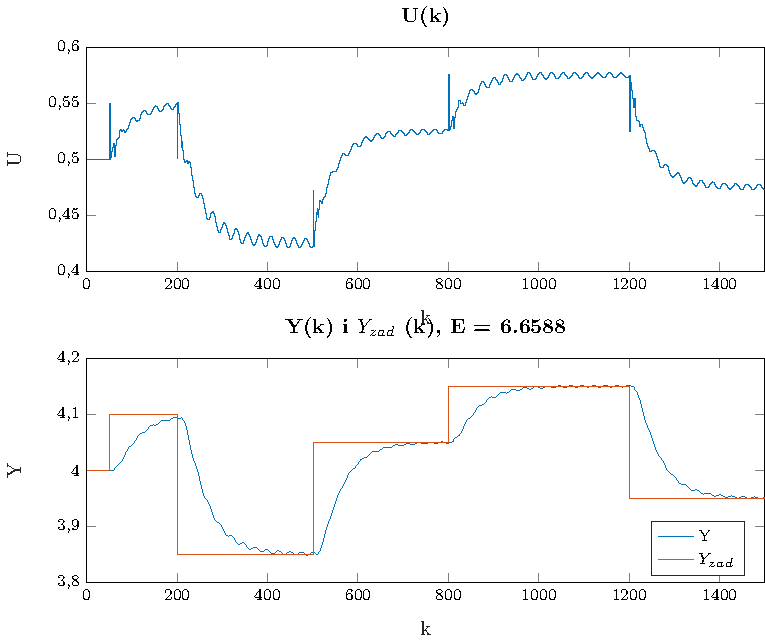
\includegraphics{../../Projekt1/rysunki_tikz/test_PID1.pdf}
	\caption{Regulator PID - test1, $K = \num{0.669}, T_\mathrm{i} = \num{18.5}, T_\mathrm{d} = \num{4.44}$ }
	\label{test-PID1}
\end{figure}

Modyfikując parametry regulatora przeprowadzone zostały jeszcze 3 eksperymenty przedstawione na rys. \ref{test-PID2}, rys. \ref{test-PID3} i rys. \ref{test-PID4}.

\begin{figure}[h]
	\centering
	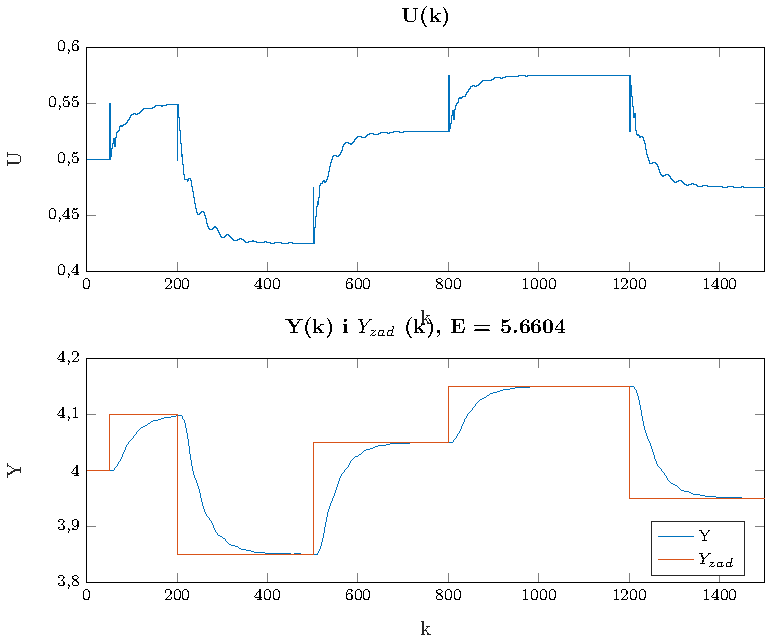
\includegraphics{../../Projekt1/rysunki_tikz/test_PID2.pdf}
	\caption{Regulator PID - test2, $K = \num{0.75}, T_\mathrm{i} = \num{16}, T_\mathrm{d} = \num{3}$}
	\label{test-PID2}
\end{figure}

\begin{figure}[h]
	\centering
	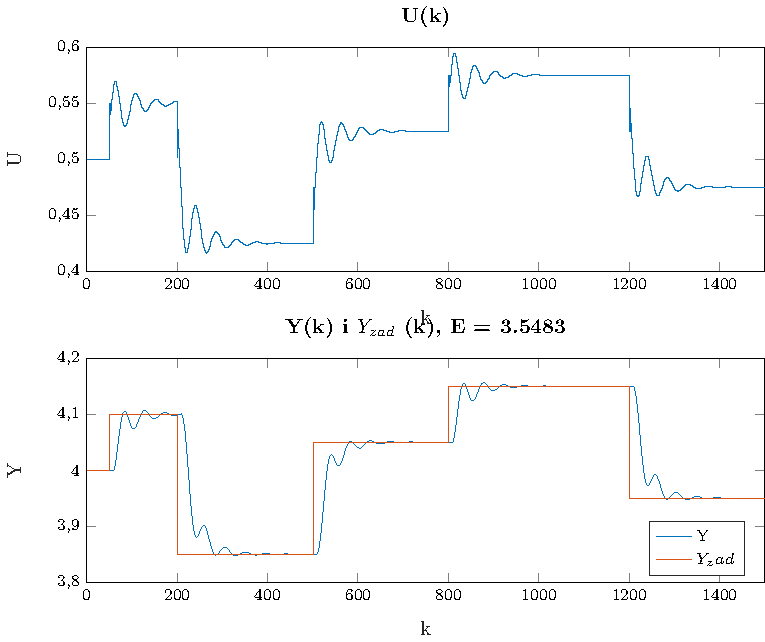
\includegraphics{../../Projekt1/rysunki_tikz/test_PID3.pdf}
	\caption{Regulator PID - test3, $K = \num{0.67}, T_\mathrm{i} = \num{10}, T_\mathrm{d} = \num{0.1}$}
	\label{test-PID3}
\end{figure}

\begin{figure}[h]
	\centering
	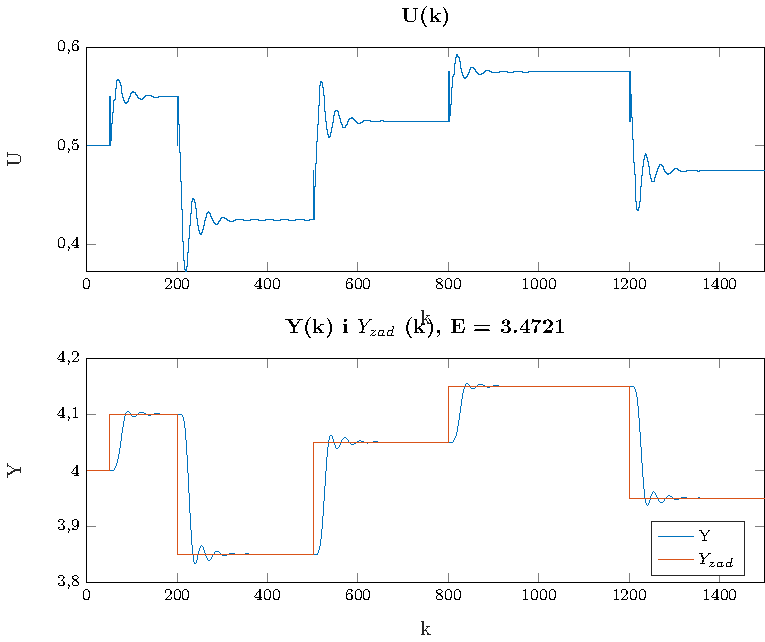
\includegraphics{../../Projekt1/rysunki_tikz/test_PID4.pdf}
	\caption{Regulator PID - test4, $K = \num{0.8}, T_\mathrm{i} = \num{7}, T_\mathrm{d} = \num{2}$}
	\label{test-PID4}
\end{figure}

Zmieniając wartości parametrów udało się poprawić regulację, zarówno zmniejszyła się wartość błędu, jak i wykresy wyglądają lepiej. Zmnniejszyły się oscylacje wyjścia procesu w momencie narastania oraz opadania sygnału do wartości zadanej. Znacząco poprawił się czas uzyskiwania wartości zadanej, nie zwiększając przy tym znacząco przesterowania.
Na tescie 3 i 4 PID działa zdecydowanie szybciej, dodatkowo oscylacje w teście 4 są zdecydowanie mniejsze.


\subsection{Nastawy DMC}

Dobór parametrów dla regulatora DMC odbywał się w podobny sposób.
W pierwszej kolejności zostały wybrane parametry w sposób przypadkowy, następnie parametry były lekko zmieniane.
Patrząc na wyniki symulacji można było wybrać najlepszy nastaw. Eksperymenty DMC zostały przedstawione na rys. \ref{test-DMC1} - \ref{test-DMC6}.
Z przeprowadzonych eksperymentów wynika, że dla parametrów: $ N = 20, N_\mathrm{u} = 3, \lambda = \num{1.5} $ wyniki regulacji są najlepsze. Dla mniejszych wartości horyzontu predykcji i sterowania wynki znacząco się pogarszają, natomiast dla większych nie jest zauważalna znacząca zmiana.

\begin{figure}[h]
	\centering
	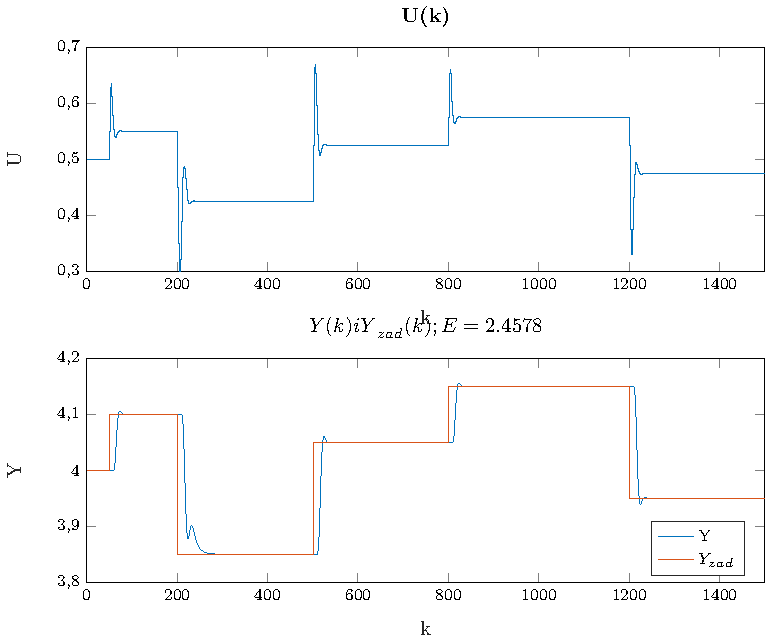
\includegraphics{../../Projekt1/rysunki_tikz/test_DMC1.pdf}
	\caption{Regulator DMC - test1, $ N = 60, N_\mathrm{u} = 40, \lambda = 1 $}
	\label{test-DMC1}
\end{figure}

\begin{figure}[h]
	\centering
	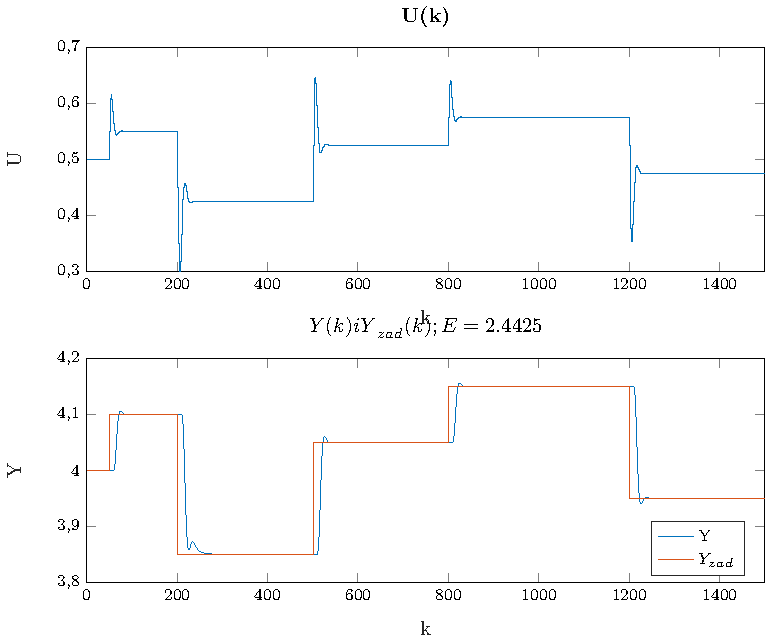
\includegraphics{../../Projekt1/rysunki_tikz/test_DMC2.pdf}
	\caption{Regulator DMC - test2, $ N = 40, N_\mathrm{u} = 20, \lambda = 2 $}
	\label{test-DMC2}
\end{figure}

\begin{figure}[h]
	\centering
	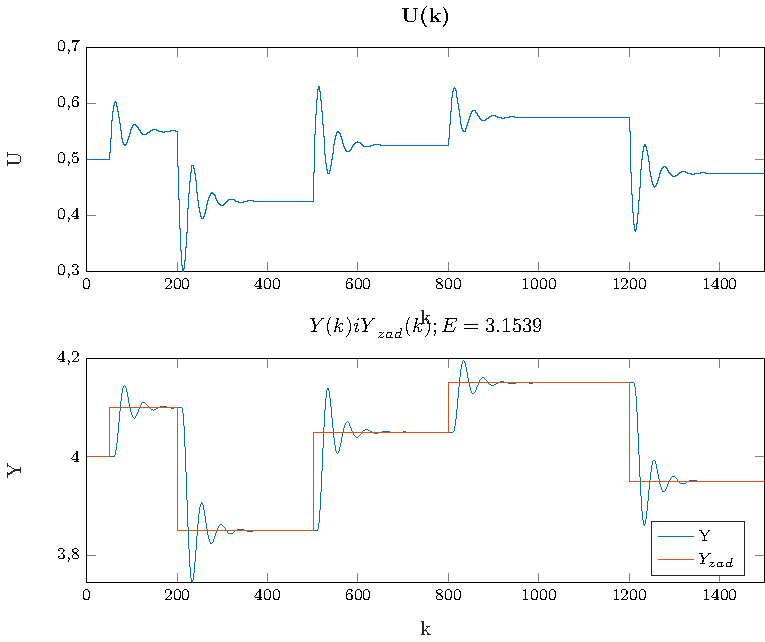
\includegraphics{../../Projekt1/rysunki_tikz/test_DMC3.pdf}
	\caption{Regulator DMC - test3, $ N = 11, N_\mathrm{u} = 1, \lambda = 1 $}
	\label{test-DMC3}
\end{figure}

\begin{figure}[h]
	\centering
	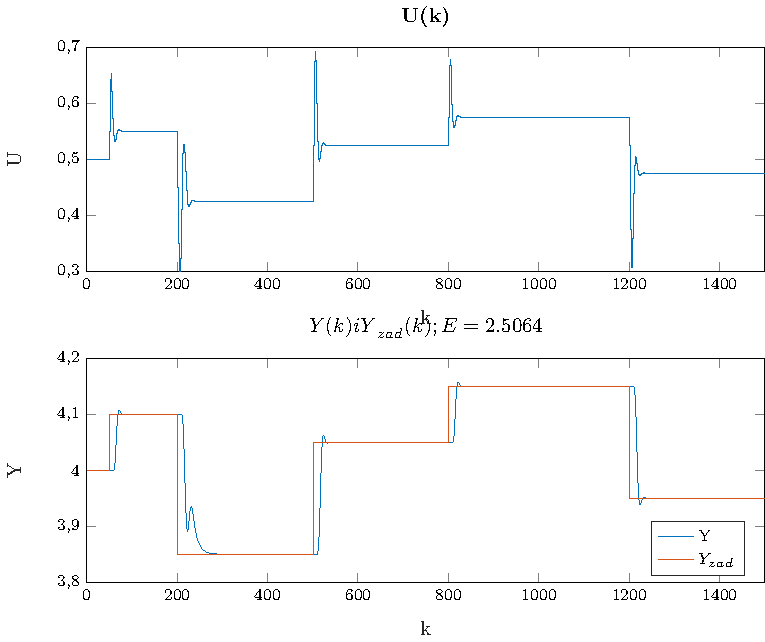
\includegraphics{../../Projekt1/rysunki_tikz/test_DMC4.pdf}
	\caption{Regulator DMC - test4, $ N = 15, N_\mathrm{u} = 1, \lambda = 1 $}
	\label{test-DMC4}
\end{figure}

\begin{figure}[h]
	\centering
	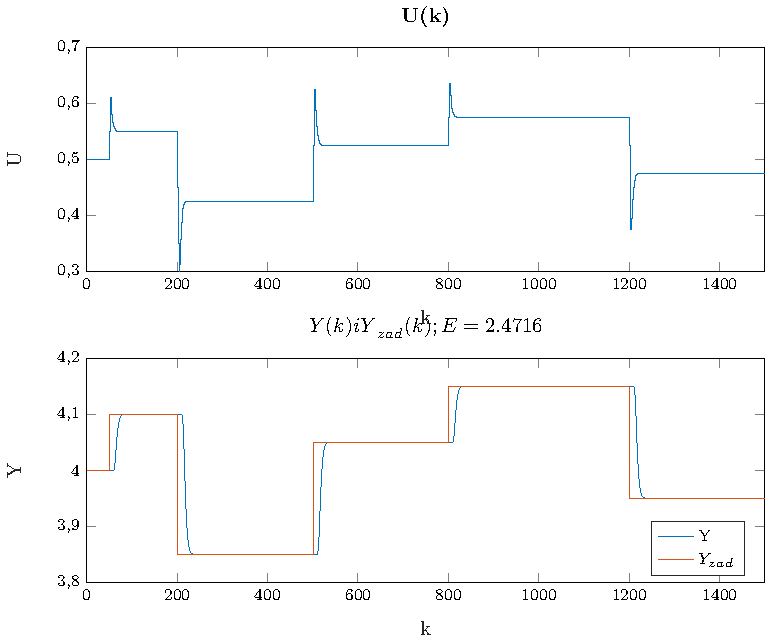
\includegraphics{../../Projekt1/rysunki_tikz/test_DMC5.pdf}
	\caption{Regulator DMC - test5, $ N = 20, N_\mathrm{u} = 1, \lambda = 1 $}
	\label{test-DMC5}
\end{figure}

\begin{figure}[h]
	\centering
	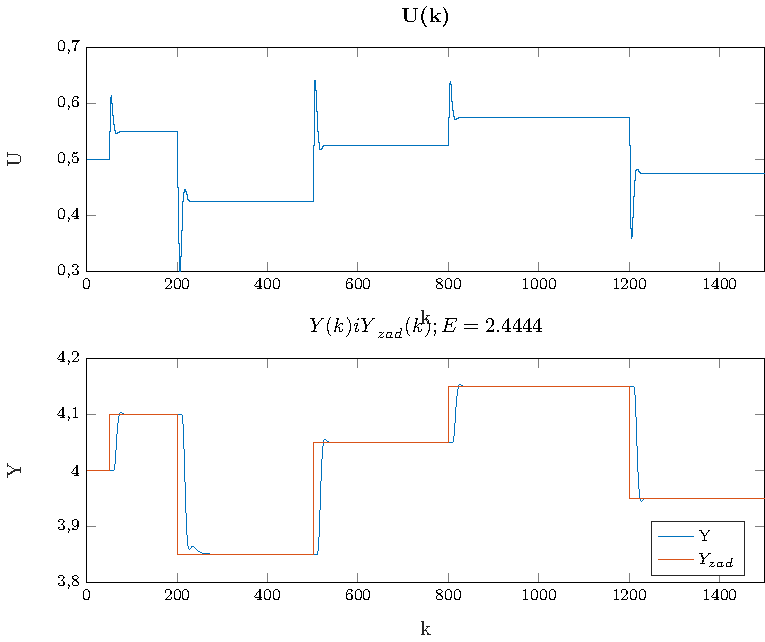
\includegraphics{../../Projekt1/rysunki_tikz/test_DMC6.pdf}
	\caption{Regulator DMC - test6, $ N = 20, N_\mathrm{u} = 3, \lambda = \num{1.5} $}
	\label{test-DMC6}
\end{figure}


\section{Dobór parametrów PID i DMC automatycznie}


W celu optymalizacji wskaźnika błędu w zależności od parametrów obu regulatorów
został użyty algorytm generyczny, którego zadaniem było znalezienie minimum funkcji błędów.

Uzyskane nastawy to:
\begin{equation}
	\begin{split}
		& \text{dla PID}: K = \num{0.8706}, T_\mathrm{i} = \num{5.6252}, T_\mathrm{d} = \num{2.9545}, E = \num{3.3250} \\
		& \text{dla DMC}: N = 19, N_\mathrm{u} = 30, \lambda = \num{1.9185}, E = \num{2.4421} \\
	\end{split}
\end{equation}

Otrzymane nastawy nie różnią się znacząco od tych uzyskanych metodą eksperymentalną, niemniej jednak błędy regulacji są mniejsze.
Wykresy regulacji dla tych nastawów są przedstawione na rys. \ref{PID-optymalizacja} i \ref{DMC-optymalizacja}.
Metoda optymalizacji jest bardziej przydatna dla regulatora PID niż DMC, ponieważ znajdując graniczne wartości N oraz $N_\mathrm{u}$ po ich dalszym zwiększaniu nie powoduje to znaczącej poprawy regulacji, zużywa jednak większe zasoby mocy obliczeniowej. Natomias dla regulatora PID znacząco oszczędza czas potrzebny na testowanie zmian nastawów metodami eksperymentalymi.

\begin{figure}[h]
	\centering
	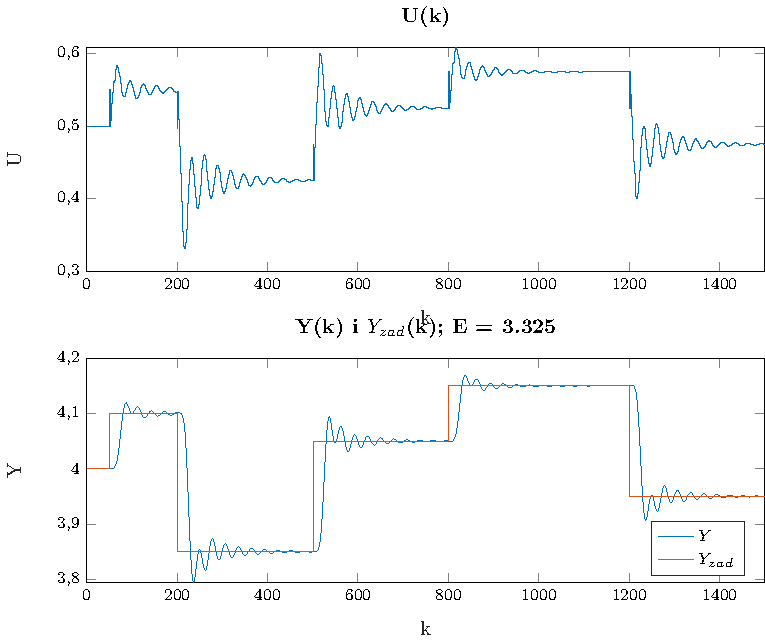
\includegraphics{../../Projekt1/rysunki_tikz/PID_optimal.pdf} %  = , Ti =  Td =; E = 3.3250
	\caption{Regulator PID - parametry wyznaczone algorytmem generycznym, $ N = 19, N_\mathrm{u} = 30, \lambda = \num{ 1.9185}, E = \num{2.4421} $}
	\label{PID-optymalizacja}
\end{figure}


\begin{figure}[h]
	\centering
	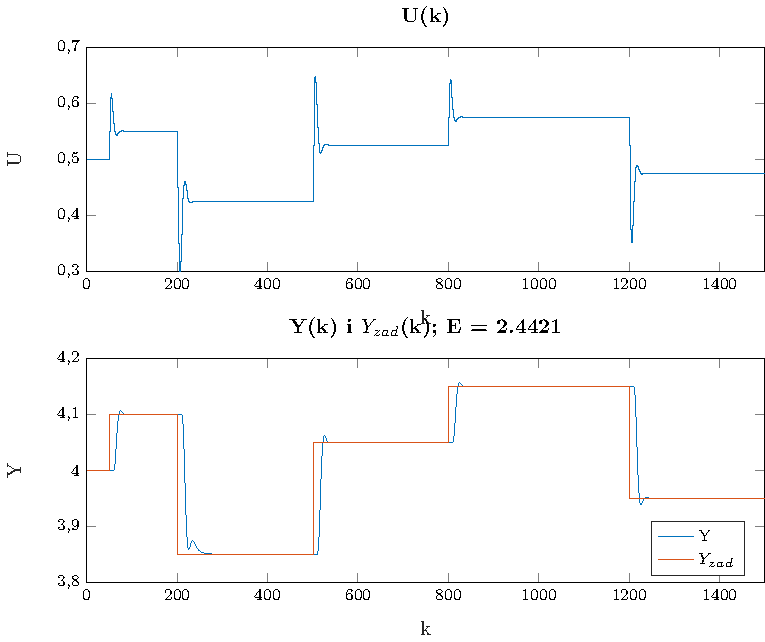
\includegraphics{../../Projekt1/rysunki_tikz/DMC_optimal.pdf} %  = , Ti =  Td =; E = 3.3250
	\caption{Regulator DMC - parametry wyznaczone algorytmem generycznym, $K = \num{0.8706}, T_\mathrm{i} = \num{5.6252}, T_\mathrm{d} = \num{2.9545}$}
	\label{DMC-optymalizacja}
\end{figure}
\end{comment}

\end{document}

